\documentclass[aspectratio=169,font=14pt]{beamer}
% \documentclass[notes=only]{beamer}
\usepackage{microtype} % Slightly tweak font spacing for aesthetics
\usepackage{mathtools}
\usepackage{etoolbox}
\usepackage{amsmath}
\usepackage[export]{adjustbox}
\usepackage{xcolor}
\usepackage{tikz}
\usepackage{graphicx}
\graphicspath{{defense/}}
\usepackage{pgfpages}
% \usepackage[style=nature,citestyle=numeric]{biblatex}
\usepackage[export]{adjustbox}
\usepackage{appendixnumberbeamer}
\usepackage{relsize}
% \usepackage[threecols]{hackthefootline}
\usepackage{tikzlings}
\usepackage{setspace}
\usepackage{ragged2e}
\usepackage[hang]{footmisc}
\usepackage{bm}
\usepackage{colortbl}
\usepackage{fontawesome}
\usetikzlibrary{shapes,arrows,calc,positioning,matrix,fit}
\usetikzlibrary{decorations,backgrounds}
\usetikzlibrary{decorations.pathreplacing,decorations.markings,decorations.pathmorphing}
\usetikzlibrary{shapes.multipart}
\usetikzlibrary{overlay-beamer-styles}
%%%%%%%%%%%%%%%%%%%%%%%%%%%%%%%%%%%%%%%%%%%5
\usepackage{url}
\urlstyle{same}
\usepackage[absolute,overlay]{textpos}
\usepackage[default]{sourcesanspro}
\usepackage{contour}
\usepackage{textcomp}
\usepackage{multirow}
\usepackage{fancyvrb}
\usepackage{ulem}
\usepackage{xpatch}
\usepackage{algpseudocode}

\usepackage{pgf}
\usepackage{alphalph}
\usepackage{fancybox}
\usetikzlibrary{calc}
%%%%%%%%%%%%%%%%%%%%%%%%%%%%%%%%%%%%%%%%%%%5

\usefonttheme{professionalfonts}
\usetheme{Boadilla}

\setbeamercolor{title}{parent=author in head/foot}

% \addbibresource{refs.bib}
\setbeamertemplate{navigation symbols}{}%remove navigation symbols
% \beamertemplatenavigationsymbolsempty
\hypersetup{pdfstartview={Fit}} % fits the presentation to the window when first displayed
% \emergencystretch=1em

% \setbeameroption{hide notes} % Only slides
% \setbeameroption{show only notes} % Only notes
% \setbeameroption{show notes on second screen=right} % Both

% Give a slight yellow tint to the notes page
% \setbeamertemplate{note page}{\pagecolor{yellow!5}\insertnote}\usepackage{palatino}

% \htfconfig{title=short, authinst=instpths, date=none, framenrs=fraction}
% \addtobeamertemplate{frametitle}{}{\vspace{-1em}} % decrease

%%%%%%%%%%%%%%%%%%%%%%%%
\newcommand{\TODO}[1]{\textcolor{red}{TODO: #1}}
\newcommand{\cyan}[1]{\textcolor{cyan}{#1}}
\newcommand*\pct{\scalebox{.9}{\%}}
\newcommand{\inlinefigure}[1]{%
  \begingroup\normalfont
  \includegraphics[height=\fontcharht\font`\B]{#1}%
  \endgroup
}
\newcommand{\grande}[1]{\mathlarger{\mathlarger{#1}}}

\setbeamertemplate{itemize items}[circle]
\setbeamertemplate{itemize item}{}
\setbeamercolor{itemize subitem}{fg=blue!75}
\setlength\leftmargini{0pt}

\makeatletter
\patchcmd{\@listI}{\itemsep3\p@ \@plus2\p@ \@minus3\p@}{\itemsep3\p@ \@plus1fill \@minus3\p@}{}{}
\makeatother
%%%%%%%%%%%%%%%%%%%%%%%%

% Title information ------------------------------------------------------------
\title[Pairwise Alignment of CDS]{\textbf{Statistical Sequence Alignment of Protein Coding Regions}}
\titlegraphic{%
\vspace*{-4em}\begin{tikzpicture}
    \draw node[anchor=south west] at ($(current page.south west)+(5mm,5mm)$)
    {\pgfimage[height=15mm]{defense/images/biodesign_logo.png}};
    \draw node[anchor=south east] at ($(current page.south east)+(-5mm,5mm)$)
    {\pgfimage[height=15mm]{defense/images/fulton_logo.png}};
\end{tikzpicture}
% \vspace{-4em}
\includegraphics[width=0.3\linewidth,height=2cm]{images/biodesign_logo.png}%
% \hspace{4cm}%
% \vspace{-4em}
\includegraphics[width=0.35\linewidth,height=2cm]{images/fulton_logo.png}%
}
\author[JJ García Mesa]{~\\%
~\\%
~\\%
Juan José García Mesa\\
~\\
~\\
{\small Reed Cartwright, chair\\
Banu Ozkan\\
Jay Taylor\\
Ted Pavlic\\}}

% \date{2023/10/25}
\date{}
% \titlegraphic{\includegraphics[width=.3\linewidth]{}}
%-------------------------------------------------------------------------------
\setbeamertemplate{footline}
{%
  \leavevmode%
  \hbox{%
  \begin{beamercolorbox}[wd=.333333\paperwidth,ht=2.25ex,dp=1ex,center]{author in head/foot}%
    \usebeamerfont{title in head/foot}\insertshortauthor
  \end{beamercolorbox}%
  \begin{beamercolorbox}[wd=.333333\paperwidth,ht=2.25ex,dp=1ex,center]{title in head/foot}%
    \usebeamerfont{title in head/foot}\insertshorttitle
  \end{beamercolorbox}%
  \begin{beamercolorbox}[wd=.333333\paperwidth,ht=2.25ex,dp=1ex,leftskip=2ex,rightskip=2ex,sep=0pt]{date in head/foot}%
    \hfill%
    \usebeamerfont{date in head/foot}%
    \raisebox{-0.1\height}{\faicon{github}}~jgarciamesa%
    \hfill%
    \usebeamercolor[fg]{page number in head/foot}%
    \usebeamerfont{page number in head/foot}%
    \usebeamertemplate{page number in head/foot}%
  \end{beamercolorbox}}%
  \vskip0pt%
}
%-------------------------------------------------------------------------------

\begin{document}
\maketitle

\begin{frame}[t]{Protein Coding Regions} %-----------------------------------------
\begin{columns}[T]
    \column{0.5\textwidth}
    \begin{itemize}
        \setlength\itemsep{1em}
        \item Coding regions (CDS) are DNA sequences that code for proteins.
        \item Proteins are chains of amino acids responsible for virtually all chemical processes in living organisms.
        \item A codon is a sequence of three nucleotides that encode a particular amino acid.
    \end{itemize}
    \centering
    \vspace{3em}
    \only<2>{\resizebox{0.9\textwidth}{!}{
\begin{tikzpicture}
  \newcommand*{\adenin}[2]{\begin{scope}[shift = {#1}, rotate = #2, fill = red]%
        \fill(0, -.1) -- (.35, -.1) -- (.45, 0) -- (.35, .1) -- (0, .1) -- cycle;%
        \node at (-0.2, 0) {A};
  \end{scope}}%
  \newcommand*{\thymin}[2]{\begin{scope}[shift = {#1}, rotate = #2, fill = blue]%
        \fill(0, -.1) -- (.35, -.1) -- (.25, 0) -- (.35, .1) -- (0, .1) -- cycle;
        \node at (-0.2, 0) {T};
  \end{scope}}%
  \newcommand*{\guanin}[2]{\begin{scope}[shift = {#1}, rotate = #2, fill = green]%
        \fill(0, -.1) -- (.35, -.1) arc(-90:90:.1) -- (.35, .1) -- (0, .1) -- cycle;%
        \node at (-0.2, 0) {G};
  \end{scope}}%
  \newcommand*{\cytosin}[2]{\begin{scope}[shift = {#1}, rotate = #2, fill = yellow]%
        \fill(0, -.1) -- (.35, -.1) arc(270:90:.1) -- (.35, .1) -- (0, .1) -- cycle;%
        \node at (-0.2, 0) {C};
  \end{scope}}%
  \newcommand*{\somein}[1]{\ifcase#1
  \or 
  \adenin{(0, 0)}{90}
  \or
  \cytosin{(0, 0)}{90}
  \or
  \guanin{(0, 0)}{90}
  \or
  \thymin{(0, 0)}{90}
  \fi
  }
  \newcommand\myinlst{0, 1, 4, 3, 3, 2, 1, 3, 1, 4, 0}
  \draw[double distance = 1pt, line cap = rect, decoration = {
        markings, 
        mark=between positions 5pt and 0.99 step 10pt
         with
        {\pgfmathtruncatemacro{\myin}{{\myinlst}[\pgfkeysvalueof{/pgf/decoration/mark info/sequence number}-1]}
         \somein{\myin}},
        % 200 more lines with at position ...
     }, preaction = {decorate}, shorten <= -3pt]
        (0, 0) -- (3.6, 0);  % Straight line
        % (-.5, -0.2) .. controls (2, 1) and (4, -1) .. (7.6, 0);
   \node at (0.9, -0.7) {\textbf{Met}};
   \draw [decorate, decoration = {brace}] (1.35,-0.4) -- (0.4,-0.4);
   \node at (1.95, -0.7) {Ala};
   \draw [decorate, decoration = {brace}] (2.4,-0.4) -- (1.45,-0.4);
   \node at (3, -0.7) {Asp};
   \draw [decorate, decoration = {brace}] (3.45,-0.4) -- (2.5,-0.4);

    \node at (4.1, 0) {$\cdots$};
   
  \renewcommand\myinlst{1, 3, 1, 4, 1, 3, 0}
    \draw[double distance = 1pt, line cap = rect, decoration = {
        markings, 
        mark=between positions 5pt and 0.99 step 10pt
         with
        {\pgfmathtruncatemacro{\myin}{{\myinlst}[\pgfkeysvalueof{/pgf/decoration/mark info/sequence number}-1]}
         \somein{\myin}},
        % 200 more lines with at position ...
     }, preaction = {decorate}, shorten <= -3pt]
        (4.7, 0) -- (7.2, 0);  % Straight line
        % (-.5, -0.2) .. controls (2, 1) and (4, -1) .. (7.6, 0);
   \node at (5.2, -0.7) {Arg};
   \draw [decorate, decoration = {brace}] (5.75,-0.4) -- (4.8,-0.4);
   \node at (6.3, -0.7) {\textbf{STOP}};
   \draw [decorate, decoration = {brace}] (6.8,-0.4) -- (5.85,-0.4);
\end{tikzpicture}}}
  \column{0.5\textwidth}
    \centering
    \includegraphics<1>[height = 0.75\textheight]{defense/images/translation.jpg}
    \includegraphics<2>[width = 0.9\textwidth]{defense/images/codon-table.png}
    \only<1>{\footnotetext{\tiny{Clancy S, Brown W (2008) Translation: DNA to mRNA to Protein}}}
    \end{columns}
\note[item]{Coding regions are DNA sequences that, through various mechanisms such as transcription and translation, code for proteins, which are chains of amino acids responsible for virtually all the chemical processes in living organisms.}
\note[item]{Codons are sets of three nucleotides that encode for amino acids.}
\note[item]{Protein coding regions start with a special start codon and end with one of three possible stop codons.}
\end{frame} %------------------------------------------------------------------

\begin{frame}{Protein Coding Regions} %----------------------------------------
\begin{columns}[T]
    \setlength{\topsep}{0pt}
    \setlength{\partopsep}{0pt}
  \column{0.3\textwidth}
    \textbf{Human Health}
    \vspace{0.8em}
    \begin{itemize}
        \item Personalized medicine
        \item Drug discovery
        \item Identification of disease-associated mutations
    \end{itemize}
    \begin{tikzpicture}[remember picture, overlay, on background layer]
        \draw node at ($(current page.center)+(-5.4cm,-2.8cm)$) {\pgfimage[height=15mm]{images/personalized.png}};
    \end{tikzpicture}
    \centering
  \column{0.35\textwidth}
    \textbf{Evolution}
    \vspace{0.8em}
    \begin{itemize}
        \item Phylogenetic inference
        \item Measurement of selection
    \end{itemize}
    \begin{tikzpicture}[remember picture, overlay, on background layer]
        \draw node at ($(current page.center)+(0cm,-2.8cm)$) {\pgfimage[height=15mm]{images/phylogenetics.png}};
    \end{tikzpicture}
  \column{0.3\textwidth}
    \textbf{Genomics}
    \vspace{0.8em}
    \begin{itemize}
        \item Gene annotation
        \item Reference mapping
    \end{itemize}
    \begin{tikzpicture}[remember picture, overlay, on background layer]
        \draw node at ($(current page.center)+(5.6cm,-2.8cm)$) {\pgfimage[height=15mm]{images/genetics.png}};
    \end{tikzpicture}
  % \column{0.6\textwidth}
  %   \centering
  %   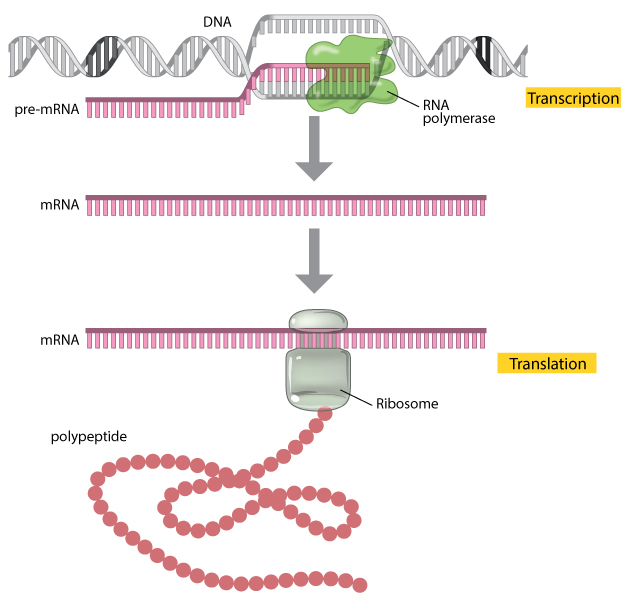
\includegraphics[height = 0.8\textheight]{defense/images/translation.jpg}
  %   % https://www.nature.com/scitable/topicpage/translation-dna-to-mrna-to-protein-393/
  %   % \includegraphics<2>[height = 0.8\textheight]{defense/images/translation-detail.jpg}
  %   \footnotetext{\tiny{Clancy S, Brown W (2008) Translation: DNA to mRNA to Protein}}
\end{columns}
\note[item]{The study of CDS is important for human health fields such as personalized medicine, drug discovery, and the identification of disease-associated mutation; used in the study of evolution such as phylogenetic inference and measurement of selection; and in genomics for gene annotation or reference mapping.}
\end{frame} %-------------------------------------------------------------------

\begin{frame}[t]{Sequence Alignment} %---------------------------------------------
\begin{columns}
\column{0.6\textwidth}
    \begin{itemize}
        \setlength\itemsep{1em}
        \item Hypothesis of which residues in two or more sequences are related by common descent.
        \item One of the most fundamental computational steps in most genomic analyses.
        \item Remains an important problem in computational biology and bioinformatics.
        % \item \textbf{How:} alignments of sequences are not observed directly and must be inferred from data using algorithms.
    \end{itemize}
\column{0.4\textwidth}
    \centering
    \definecolor{colorY}{RGB}{255,255,51}   % YELLOW
\definecolor{colorG}{RGB}{77,175,74}    % GREEN
\definecolor{colorB}{RGB}{55,126,184}   % BLUE
\definecolor{colorR}{RGB}{228,26,28}    % RED
\definecolor{colorGy}{RGB}{153,153,153} % GRAY
\definecolor{colorP}{RGB}{152,78,163}   % PURPLE

\begin{tikzpicture}[node distance=1mm,font=\footnotesize]
\tikzstyle{aln}=[matrix of nodes, nodes in empty cells,fill=colorGy!20]
\newcommand{\A}{\textcolor{colorP}{\textbf{A}}}
\newcommand{\C}{\textcolor{colorG}{\textbf{C}}}
\newcommand{\G}{\textcolor{colorB}{\textbf{G}}}
\newcommand{\T}{\textcolor{colorY}{\textbf{T}}}

\matrix (msa)[aln] {
% \C\A\T & \A\A\G & \C\G\G & \T\C\G & \G\A\C & \verb|---|\\
\C\A\G & \C\A\G & \C\G\G & \T\C\G & \G\A\C & \A\C\G\\
\C\A\T & \C\A\G & \C\G\G & \T\C\verb|-| & \verb|--|\C & \A\C\A\\
% \C\A\T & \C\A\G & \C\C\G & \T\C\G & \G\A\C & \A\C\G\\
};
\end{tikzpicture}
\end{columns}
\vspace{2em}
\begin{block}{\textbf{Goal}}
    Reduce errors in sequence alignment to improve downstream analyses.
\end{block}
\note[item]{Sequence alignment is the hypothesis of which residues in 2 or more sequences are related by common descent and is a fundamental step in genomic analyses, including the ones I just mentioned.}
\note[item]{Alignments of sequences are not observed directly and must be inferred from data using algorithms, which can introduce errors that impact the results of downstream analyses.}
\note[item]{The goal of this project is to reduce errors. Let me illustrate some of the issues of current aligners with an example.}
\end{frame} %-------------------------------------------------------------------

\begin{frame} %--------------------------------------------------------
\newcommand{\gap}{\rule[0.22em]{1.25em}{0.9pt}}
\newcommand{\e}[1]{\textbf{\textcolor{red}{#1}}}
% \tikzset{ser/.style={fill=cbColorO}} % s=5
% \tikzset{his/.style={}} % h=5
% \tikzset{lys/.style={}} % k=5
% \tikzset{gly/.style={}} % g=6
% \tikzset{arg/.style={}} % r=5
% \tikzset{asp/.style={}} % d=5
% \tikzset{ala/.style={}} % a=5
% \tikzset{gln/.style={}} % q=5
% \tikzset{thr/.style={}} % t=5

\tikzset{aaaln/.style={
  matrix of nodes,
  nodes in empty cells,
  nodes={text width=8mm,align=center},
  column 1/.style={nodes={align=right}}
}}
\large\centering%
\begin{tikzpicture}

\matrix[aaaln] at (0,0) {
  A: & SER & HIS &  LYS & GLY & ARG & SER & \gap & ASP & ALA & \gap \\
  D: & SER & \e{GLN} & \gap & GLY & ARG & SER &  PRO & ASP & ALA & THR \\
};

\matrix[aaaln,visible on=<2->,row 3/.style={nodes={align=right}}] at (0, -2.5) {
  A: & TCC & CAT &  AAG & GGG & CGG & TCG & ––– & GAC & GCC & –––\\
  D: & TCC & CA\e{G} &  ––– & GGG & CGG & TC\e{C} &  CCG & GAC & GCC & ACG \\
};

\matrix[aaaln,visible on=<3->] at (0, -5) {
  A: & TCC & CAT & AAG & GGG & CGG & T––\, & –CG & GAC & GCC & –––\\
  D: & TCC & CA– & ––G & GGG & CGG & TCC & CCG & GAC & GCC & ACG \\
};

\end{tikzpicture}
\note[item]{Here, we have an alignment of amino acids with some insertions and deletions and one mismatch (in red).}
\note[item]{Now, let's look at the DNA level. We have another (synonymous) mismatch!}
\note[item]{If we now consider the alignment at the DNA level, we can find a better alignment without mismatches.}
\note[item]{It's important to look at the DNA level.}
\end{frame} %-------------------------------------------------------------------

\begin{frame} %--------------------------------------------------------
%%% Okabe Ito set
\definecolor{cbColorO}{RGB}{230,159,0}
\definecolor{cbColorSb}{RGB}{86,180,233}
\definecolor{cbColorBg}{RGB}{0,158,115}
\definecolor{cbColorY}{RGB}{240,228,66}
\definecolor{cbColorBu}{RGB}{0,114,178}
\definecolor{cbColorV}{RGB}{213,94,0}
\definecolor{cbColorRp}{RGB}{204,121,167}
\definecolor{cbColorBk}{RGB}{0,0,0}
%%%%%%%%%%%%%%%%%%%%%%%%

\newcommand{\gap}{\rule[0.22em]{1.25em}{0.9pt}}
\tikzset{aaaln/.style={
  matrix of nodes,
  nodes in empty cells,
  nodes={text width=8mm,align=center},
  column 1/.style={nodes={align=right}}
}}
\large\centering%
\begin{tikzpicture}

\matrix (table) [aaaln] at (0,0) {
   &     &|[fill=cbColorSb]|\phantom{|} &|[fill=cbColorSb]|\phantom{|}      &     & &
   |[fill=cbColorV]|\phantom{|} & |[fill=cbColorV]|\phantom{|} &     &     & |[fill=cbColorRp,text width=16mm]|\phantom{|} \\
   & ser & his &  lys & gly & arg & \phantom{gly} & \phantom{gly} & asp & ala & \phantom{gly} \\
A: & TCC & CAT & AAG & GGG & CGG & T––\, & –CG & GAC & GCC & –––\\[1ex]
D: & TCC & CA– & ––G & GGG & CGG & TCC & CCG & GAC & GCC & ACG \\
   & ser & \phantom{gly} & \phantom{gly}  & gly & arg & ser & pro & asp & ala & thr \\
   % &     &\phantom{|} &\phantom{|}      &     & &
   % \phantom{|} & \phantom{|} &     &     & \phantom{|} \\
};

\node[fit=(table-2-7)(table-2-8),inner sep=0pt] (a) {};
\node[fit=(table-5-3)(table-5-4),inner sep=0pt] (b) {};
\node[fit=(table-1-3)(table-1-4),inner sep=0pt] (p2) {};
\node[fit=(table-1-7)(table-1-8),inner sep=0pt] (p1) {};
\node[fit=(table-1-11),inner sep=0pt] (p0) {};
% \node[fit=(table-6-3)(table-6-4),inner sep=0pt] (t2) {};
% \node[fit=(table-6-7)(table-6-8),inner sep=0pt] (t1) {};
% \node[fit=(table-6-11),inner sep=0pt] (t0) {};


\node at (a) {ser};
\node at (b) {gln};
\node[fill=cbColorSb,text=white] at (p2) {phase 2};
\node[fill=cbColorV,text=white] at (p1) {phase 1};
\node[fill=cbColorRp,text=white] at (p0) {phase 0};
% \node[fill=cbColorSb,text=white] at (t2) {type ii};
% \node[fill=cbColorV,text=white] at (t1) {type i};
% \node[fill=cbColorRp,text=white] at (t0) {type i};

\tikzset{abox/.style={inner sep=0pt,ultra thick,rounded corners=1mm}}

\node[fit=(table-1-3)(table-5-4),abox,draw=cbColorSb] {};
\node[fit=(table-1-7)(table-5-8),abox,draw=cbColorV] {};
\node[fit=(table-1-11)(table-5-11),abox,draw=cbColorRp] {};


\end{tikzpicture}
\note[item]{The indel phases are categorized based on their position, phase 0 takes an entire codon, phases 1 and 2 start after 1 or two nucleotides, respectively.}
\note[item]{This is why it's important to look at the nucleotide level.}
\end{frame} %-------------------------------------------------------------------

\begin{frame}{Artifacts in Genomic Data} %--------------------------------------
\begin{columns}
    \column{0.4\textwidth}
    Existing alignments have issues when aligning CDS in the presence of \textbf{artifacts}, common in non-model organisms.
    \vspace{1em}
    \begin{itemize}
    \setlength\itemsep{1em}
        \item Based on amino acid translations
        \item Only model phase 0 indels
        \item Trouble with early stop codons
        \item Lack a statistical model
    \end{itemize}
    \column{0.6\textwidth}
    \hspace{-6mm}\resizebox{\textwidth}{!}{% !TEX program=lualatex
\definecolor{colorR}{RGB}{228,26,28}    % RED
\definecolor{colorB}{RGB}{55,126,184}   % BLUE
\definecolor{colorG}{RGB}{77,175,74}    % GREEN
\definecolor{colorP}{RGB}{152,78,163}   % PURPLE
\definecolor{colorO}{RGB}{255,127,0}    % ORANGE
\definecolor{colorY}{RGB}{255,255,51}   % YELLOW
\definecolor{colorBn}{RGB}{166,86,40}   % BROWN
\definecolor{colorPk}{RGB}{247,129,191} % PINK
\definecolor{colorGy}{RGB}{153,153,153} % GRAY
\definecolor{asublue}{RGB}{0,163,224}
%%% Okabe Ito set
\definecolor{cbColorO}{RGB}{230,159,0}
\definecolor{cbColorSb}{RGB}{86,180,233}
\definecolor{cbColorBg}{RGB}{0,158,115}
\definecolor{cbColorY}{RGB}{240,228,66}
\definecolor{cbColorBu}{RGB}{0,114,178}
\definecolor{cbColorV}{RGB}{213,94,0}
\definecolor{cbColorRp}{RGB}{204,121,167}
\definecolor{cbColorBk}{RGB}{0,0,0}
%%%%%%%%%%%%%%%%%%%%%%%%

\tikzstyle{aln}=[matrix of nodes, nodes in empty cells]
%\tikzstyle{best}=[fill=asublue!20,rounded corners]
\tikzstyle{best}=[rounded corners]
\tikzstyle{lab}=[font=\normalsize]
\tikzstyle{indel}=[ultra thick, rounded corners]
\tikzstyle{phase0}=[draw=cbColorRp]
\tikzstyle{phase1}=[draw=cbColorV]
\tikzstyle{phase2}=[draw=cbColorSb]

\newcommand{\e}[1]{\textbf{\textcolor{colorR}{#1}}}

% \begin{document}
\begin{tikzpicture}[node distance=5mm,font=\footnotesize]

\node (titleBiology) {\textbf{Biology}};
% biology
\matrix (biology)[aln,best,above right=-2.4cm and -1.2cm of titleBiology.west] {
   & ser & his & lys & gly & arg &            &            & asp & ala & \\
A: & TCC & CAT & AAG & GGG & CGG & T\verb|--| & \verb|-|CG & GAC & GCC & \verb|---|\\
D: & TCC & CA\verb|-| & \verb|--|G & GGG & CGG & TCC & CCG & GAC & GCC & ACG\\
   & ser &            &            & gly & arg & ser & pro & asp & ala & thr\\
};
\node (bio17) [fit=(biology-1-7)(biology-1-8)]{Ser};
\node [fit=(biology-4-3)(biology-4-4)]{Gln};
\draw [indel,phase1] (biology-2-7.north west) rectangle (biology-3-8.south east);
\draw [indel,phase0] (biology-2-11.north west) rectangle (biology-3-11.south east);
\draw [indel,phase2] (biology-2-3.north west) rectangle (biology-3-4.south east);

% \node (titlePrankMacse) [below right=2.6cm and -1.8cm of titleBiology] {\textbf{b) PRANK (codon) and MACSE}};
\node (titlePrankMacse) [below right=2.4cm and -1.3cm of titleBiology] {\textbf{PRANK (codon) and MACSE}};
% prank codon --gaprate=0.01
\matrix (prank-macse) [aln,above right=-2.4cm and -1.2cm of titlePrankMacse.west] {
   & ser & his     & lys & gly  & arg & ser &           & asp & ala & \\
A: & TCC & CAT     & AAG & GGG  & CGG & TCG &\verb|---| & GAC & GCC & \verb|---|\\
D: & TCC & CA\e{G} & \verb|---| & GGG & CGG & TC\e{C} & CCG & GAC & GCC & ACG\\
   & ser & gln     &            & gly     & arg & ser   & pro  & asp & ala & thr\\
};
\draw [indel,phase0] (prank-macse-2-8.north west) rectangle (prank-macse-3-8.south east);
\draw [indel,phase0] (prank-macse-2-11.north west) rectangle (prank-macse-3-11.south east);
\draw [indel,phase0] (prank-macse-2-4.north west) rectangle (prank-macse-3-4.south east);

\node (titleMafftClustalo) [below right=2.4cm and -4cm of titlePrankMacse] {\textbf{MAFFT and Clustal$\pmb{\Omega}$}};
% mafft dna & clustalo amino acids
\matrix(mafft-clustalo) [aln,above right=-2.4cm and -1.2cm of titleMafftClustalo.west] {
   & ser & his     & lys     & gly     & arg     & ser & asp & ala & \\
A: & TCC & CAT & AAG & GGG     & CGG     & TCG & GAC & GCC & \verb|---|\\
D: & TCC & CA\e{G}     & \e{GG}G     & \e{C}GG & \e{TCC} & \e{C}CG & GAC & GCC & ACG\\
   & ser & gln     & gly     & arg     & ser     & pro & asp & ala & thr\\
};
\draw [indel,phase0] (mafft-clustalo-2-10.north west) rectangle (mafft-clustalo-3-10.south east);

% \node (titleCoati) [below right=2.4cm and -3cm of titleMafftClustalo] {\textbf{COATi}};
% % coati mar-mg
% \matrix (coati) [aln,best,above right=-2.4cm and -1.2cm of titleCoati.west] {
%    & Ser & His & Lys & Gly & Arg &            &            & Asp & Ala & \\
% A: & TCC & CAT & AAG & GGG & CGG & T\verb|--| & \verb|-|CG & GAC & GCC & \verb|---|\\
% D: & TCC & CA\verb|-| & \verb|--|G & GGG & CGG & TCC & CCG & GAC & GCC & ACG\\
%    & Ser &            &            & Gly & Arg & Ser & Pro & Asp & Ala & Thr\\
% };
% \node (cti17) [fit=(coati-1-7)(coati-1-8)]{Ser};
% \node [fit=(coati-4-3)(coati-4-4)]{Gln};
% \draw [indel,phase1] (coati-2-7.north west) rectangle (coati-3-8.south east);
% \draw [indel,phase0] (coati-2-11.north west) rectangle (coati-3-11.south east);
% \draw [indel,phase2] (coati-2-3.north west) rectangle (coati-3-4.south east);

%%%%%

% \draw (a.north west) node[lab,anchor=center] (dlab) {\textbf{a)}};
% \draw (dlab |- c.north west) node[lab,anchor=center] {\textbf{b)}};

% \node[] () [below = 0.2em] at (coati.south) {};

\end{tikzpicture}
% \end{document}
}
\end{columns}

\note[item]{Current coding sequence aligners don't model correctly within codon
	gaps and frameshifts because generally alns are done based on amino acid
	translations.}
\note[item]{Errors can impact downstream analyses and their conclusions.}
\note[item]{Comment on the alignments by the different tools.}
\end{frame} %-------------------------------------------------------------------

\begin{frame}{COATi} %--------------------------------------------------
    COdon-aware Alignment Transducer
\begin{columns}[c]
    % \setstretch{1.5}
    \column{0.4\textwidth}
    \vspace{1em}
    \begin{itemize}
    \setlength\itemsep{1em}
        \item Codon evolution
        \item Indel model --- all phases
        \item Models artifacts
        \item Finite state transducers
    \end{itemize}
    \column{0.6\textwidth}
    \hspace{-4mm}\resizebox{\textwidth}{!}{% !TEX program=lualatex
\definecolor{colorR}{RGB}{228,26,28}    % RED
\definecolor{colorB}{RGB}{55,126,184}   % BLUE
\definecolor{colorG}{RGB}{77,175,74}    % GREEN
\definecolor{colorP}{RGB}{152,78,163}   % PURPLE
\definecolor{colorO}{RGB}{255,127,0}    % ORANGE
\definecolor{colorY}{RGB}{255,255,51}   % YELLOW
\definecolor{colorBn}{RGB}{166,86,40}   % BROWN
\definecolor{colorPk}{RGB}{247,129,191} % PINK
\definecolor{colorGy}{RGB}{153,153,153} % GRAY
\definecolor{asublue}{RGB}{0,163,224}
%%% Okabe Ito set
\definecolor{cbColorO}{RGB}{230,159,0}
\definecolor{cbColorSb}{RGB}{86,180,233}
\definecolor{cbColorBg}{RGB}{0,158,115}
\definecolor{cbColorY}{RGB}{240,228,66}
\definecolor{cbColorBu}{RGB}{0,114,178}
\definecolor{cbColorV}{RGB}{213,94,0}
\definecolor{cbColorRp}{RGB}{204,121,167}
\definecolor{cbColorBk}{RGB}{0,0,0}
%%%%%%%%%%%%%%%%%%%%%%%%

\tikzstyle{aln}=[matrix of nodes, nodes in empty cells]
%\tikzstyle{best}=[fill=asublue!20,rounded corners]
\tikzstyle{best}=[rounded corners]
\tikzstyle{lab}=[font=\normalsize]
\tikzstyle{indel}=[ultra thick, rounded corners]
\tikzstyle{phase0}=[draw=cbColorRp]
\tikzstyle{phase1}=[draw=cbColorV]
\tikzstyle{phase2}=[draw=cbColorSb]

\newcommand{\e}[1]{\textbf{\textcolor{colorR}{#1}}}

% \begin{document}
\begin{tikzpicture}[node distance=5mm,font=\footnotesize]

\node (titleBiology) {\textbf{Biology}};
% biology
\matrix (biology)[aln,best,above right=-2.4cm and -1.2cm of titleBiology.west] {
   & ser & his & lys & gly & arg &            &            & asp & ala & \\
A: & TCC & CAT & AAG & GGG & CGG & T\verb|--| & \verb|-|CG & GAC & GCC & \verb|---|\\
D: & TCC & CA\verb|-| & \verb|--|G & GGG & CGG & TCC & CCG & GAC & GCC & ACG\\
   & ser &            &            & gly & arg & ser & pro & asp & ala & thr\\
};
\node (bio17) [fit=(biology-1-7)(biology-1-8)]{Ser};
\node [fit=(biology-4-3)(biology-4-4)]{Gln};
\draw [indel,phase1] (biology-2-7.north west) rectangle (biology-3-8.south east);
\draw [indel,phase0] (biology-2-11.north west) rectangle (biology-3-11.south east);
\draw [indel,phase2] (biology-2-3.north west) rectangle (biology-3-4.south east);

\node (titleCoati) [below right=2.4cm and -1.3cm of titleBiology] {\textbf{COATi}};
% coati mar-mg
\matrix (coati) [aln,best,above right=-2.4cm and -1.2cm of titleCoati.west] {
   & ser & his & lys & gly & arg &            &            & asp & ala & \\
A: & TCC & CAT & AAG & GGG & CGG & T\verb|--| & \verb|-|CG & GAC & GCC & \verb|---|\\
D: & TCC & CA\verb|-| & \verb|--|G & GGG & CGG & TCC & CCG & GAC & GCC & ACG\\
   & ser &            &            & gly & arg & ser & pro & asp & ala & thr\\
};
\node (cti17) [fit=(coati-1-7)(coati-1-8)]{Ser};
\node [fit=(coati-4-3)(coati-4-4)]{Gln};
\draw [indel,phase1] (coati-2-7.north west) rectangle (coati-3-8.south east);
\draw [indel,phase0] (coati-2-11.north west) rectangle (coati-3-11.south east);
\draw [indel,phase2] (coati-2-3.north west) rectangle (coati-3-4.south east);

%%%%%

% \draw (a.north west) node[lab,anchor=center] (dlab) {\textbf{a)}};
% \draw (dlab |- c.north west) node[lab,anchor=center] {\textbf{b)}};

\end{tikzpicture}
% \end{document}
}
    \vspace{2em}
\end{columns}
\begin{tikzpicture}[remember picture, overlay, on background layer]
    \draw node at ($(current page.center)+(-1.6cm,-2.7cm)$) {\pgfimage[height=30mm]{images/coati_psf.jpg}};
\end{tikzpicture}
\note[item]{I developed COATi, a statistical aligner that incorporates a codon evolution model, an indel model that allows gaps of all phases, models artifacts such as early stop codons, and is based on finite state transducers (more on that in the next slides).}
\note[item]{COATi, which are also cute mammals native to south and central america and the southwest US, can find the most parsimonius alignment.}
\end{frame} %-------------------------------------------------------------------

% \begin{frame}{Notation} %-------------------------------------------------------
% \begin{itemize}
%     \setlength\itemsep{1em}
%     \item \textbf{DNA alphabet}: $\grande{\Sigma}_{DNA} = \{A, C, G, T\}$.
%     \item \textbf{Codon alphabet}: $\grande{\Sigma}_{codon}$ all three-mers in $\grande{\Sigma}_{DNA}$,
%     where $X \in \grande{\Sigma}_{codon} = \{X_0 X_1 X_2\}$.
%     \item \textbf{Sequence}: finite succession of symbols in $\grande{\Sigma}$. Sequence $s$ of length $m$ is represented $s_0s_1 \cdots s_{m-1}$.
% \end{itemize}
% \end{frame} %-------------------------------------------------------------------

\begin{frame}{Statistical Alignment} %------------------------------------------
\begin{columns}[c]
  \column{0.4\textwidth}
    Typical statistical pairwise alignment uses \textbf{pair-hidden Markov models} (pair-HMMs).
    \vspace{1em}
    \begin{itemize}
    \setlength\itemsep{1em}
        \item Generate two sequences from an unknown ancestor.
        \item Alignment represents the probability that the sequences are related.
        \item Moore machine with states that emit symbols to two output tapes $(s_i, v_j)$.
    \end{itemize}
  \column{0.6\textwidth}
    \resizebox{\textwidth}{!}{% % !TEX program=lualatex
\definecolor{colorR}{RGB}{228,26,28}    % RED
\definecolor{colorB}{RGB}{55,126,184}   % BLUE
\definecolor{colorG}{RGB}{77,175,74}    % GREEN
\definecolor{colorP}{RGB}{152,78,163}   % PURPLE
\definecolor{colorO}{RGB}{255,127,0}    % ORANGE
\definecolor{colorY}{RGB}{255,255,51}   % YELLOW
\definecolor{colorBn}{RGB}{166,86,40}   % BROWN
\definecolor{colorPk}{RGB}{247,129,191} % PINK
\definecolor{colorGy}{RGB}{153,153,153} % GRAY

\tikzstyle{line}=[draw, -stealth', very thick]
\tikzstyle{block}=[circle,fill=colorB!50,on grid,font=\large]
\tikzstyle{lab}=[]
\tikzstyle{w}=[lab,midway]
\tikzstyle{e}=[lab,midway,auto=false,fill=colorP!50,font=\scriptsize]

\begin{tikzpicture}[node distance=40mm, auto,
	dottedline/.style = {ultra thick, loosely dotted,shorten >=1mm, shorten <=1mm}]
%%% Legend

%%% Indel FST
\node[block,align=center] (M) {\textbf{M}\\$s_i,v_j$};
\node[block,above right=25mm and 25mm of M,align=center] (I) {\textbf{I}$_v$\\$-,v_j$};
\node[block,below right=25mm and 25mm of M,align=center] (D) {\textbf{I}$_s$\\$s_i,-$};

\draw[line] (M) to[out=90,in=180] node[w,left=5mm] {$\delta$} (I);
\draw[line] (I) to[out=270,in=10] node[w,right=2mm] {$1-\varepsilon$} (M);

\draw[line] (M) to[out=270,in=180] node[w,left=5mm] {$\delta$} (D);
\draw[line] (D) to[out=90,in=350] node[w,right=2mm] {$1-\varepsilon$} (M);

\draw[line] (M.135) arc (45:302:8mm) node[w,left] {$1-2\delta$};
\draw[line] (I.45) arc (135:-120:8mm) node[w,right] {$\varepsilon$};
\draw[line] (D.45) arc (135:-122:8mm) node[w,right] {$\varepsilon$};

\node[font=\footnotesize,text width=50mm,below right=3cm and -2.2cm of M] (sequences) {
\begin{tabular}{r@{\,: }l}
\multicolumn{2}{l}{\textbf{Sequences}}\\
    \hline
	% X & input nucleotides\\
	% Y & intermediate nucleotides\\
	$s,v$ & output sequences\\
	% \O & nothing/empty sequence\\
\end{tabular}
};

\node[font=\footnotesize,above right=-1.45cm and -1.5cm of sequences,text width=50mm] {
\begin{tabular}{r@{\,: }l}
\multicolumn{2}{l}{\textbf{Parameters}}\\
\hline
	$\delta$ & gap open weight\\
	$\varepsilon$ & gap extension weight\\
\end{tabular}
};


\end{tikzpicture}}
    \footnotetext{\tiny{Do CB et al., ProbCons: Probabilistic consistency-based multiple sequence alignment}}
\end{columns}
\note[item]{Statistical alignment, which uses models that assign probabilities to evolutionary events, is typically done using pair-hidden Markov models.}
\note[item]{Generate 2 sequences from un unknown ancestor and the alignment represents the probability that the sequences are related.}
\note[item]{Describe figure; moore machine with states match, insertion, and deletion that emit symbols (nucleotides or amino acids) to two output tapes (the two sequences).}
\note[item]{Extra info: Markov process is a stochastic model describing a sequence of possible events in which the probability of each event depends only on the state attained in the previous event.}
\end{frame} %-------------------------------------------------------------------

\begin{frame}{Finite State Transducers} %---------------------------------------
\begin{columns}
    \column{0.5\textwidth}
    \vspace{1em}
    \begin{itemize}
        \setlength\itemsep{0.75em}
        \item FSTs have similar benefits to pair-HMMs in addition to well-defined algorithms for combining them.
        \item Generates a descendant sequence given an ancestral one.
    \end{itemize}
    \column{0.5\textwidth}
    \begin{itemize}
        \setlength\itemsep{0.75em}
        \item Alignment represents the conditional probability that sequence $v$ evolved from $s$.
        \item Mealy machine with arcs that absorbs symbols from input tape and emits to output tape $(s_i:v_j)$.
    \end{itemize}
\end{columns}
\vfill
\centering
\hspace*{-3em}\resizebox{0.8\textwidth}{!}{\definecolor{colorR}{RGB}{228,26,28}    % RED
\definecolor{colorB}{RGB}{55,126,184}   % BLUE
\definecolor{colorG}{RGB}{77,175,74}    % GREEN
\definecolor{colorP}{RGB}{152,78,163}   % PURPLE
\definecolor{colorO}{RGB}{255,127,0}    % ORANGE
\definecolor{colorY}{RGB}{255,255,51}   % YELLOW
\definecolor{colorBn}{RGB}{166,86,40}   % BROWN
\definecolor{colorPk}{RGB}{247,129,191} % PINK
\definecolor{colorGy}{RGB}{153,153,153} % GRAY

\tikzstyle{line}=[draw, -stealth', very thick]
\tikzstyle{block}=[circle,fill=colorB!50,on grid]
\tikzstyle{lab}=[]
\tikzstyle{w}=[lab,midway]
\tikzstyle{e}=[lab,midway,below=-4mm,auto=false,font=\small]

% \begin{document}
% \begin{tikzpicture}[node distance=25mm, auto]
\begin{tikzpicture}[node distance=25mm, auto,
	dottedline/.style = {ultra thick, loosely dotted,shorten >=1mm, shorten <=1mm}]

% complimenting FST
\node (titlea) {};

\node[block,below left=0.75cm and 2cm of titlea.west,fill=colorG!50] (start1) {start};
\node[block,right=15mm of start1,minimum size=20pt] (cod0) {};
\node[block,right=20mm of cod0,minimum size=20pt] (cod1) {};
\node[block,right=20mm of cod1,minimum size=20pt] (cod2) {};
\node[block,right=20mm of cod2,minimum size=20pt] (cod3) {};
\node[block,fill=colorR!50,right=15mm of cod3] (end1) {end};

\draw[line] (start1) -- (cod0);
\draw[line] (cod3) -- (end1);

\draw[line] (cod0) to[bend right=-60] node[e] {A:T} (cod1);
\draw[line] (cod0) to[bend right=-25] node[e] {C:G} (cod1);
\draw[line] (cod0) to[bend right=25] node[e,below=-4.5mm] {G:C} (cod1);
\draw[line] (cod0) to[bend right=60] node[e] {T:A} (cod1);

\draw[line] (cod1) to[bend right=-60] node[e] {A:T} (cod2);
\draw[line] (cod1) to[bend right=-25] node[e] {C:G} (cod2);
\draw[line] (cod1) to[bend right=25] node[e,below=-4.5mm] {G:C} (cod2);
\draw[line] (cod1) to[bend right=60] node[e] {T:A} (cod2);

\draw[line] (cod2) to[bend right=-60] node[e] {A:T} (cod3);
\draw[line] (cod2) to[bend right=-25] node[e] {C:G} (cod3);
\draw[line] (cod2) to[bend right=25] node[e,below=-4.5mm] {G:C} (cod3);
\draw[line] (cod2) to[bend right=60] node[e] {T:A} (cod3);

\end{tikzpicture}}
\note[item]{Read points.}
\note[item]{Here I have an example of an FST that produces the DNA complement of a codon.}
\end{frame} %-------------------------------------------------------------------

\begin{frame}[c]{Finite State Transducers} %------------------------------------
\vspace{1em}
{\centering
% \only<1>{\resizebox{\textwidth}{!}{\definecolor{colorR}{RGB}{228,26,28}    % RED
\definecolor{colorB}{RGB}{55,126,184}   % BLUE
\definecolor{colorG}{RGB}{77,175,74}    % GREEN

\tikzstyle{line}=[draw, -stealth', very thick, black]
\tikzstyle{block}=[circle,fill=colorB!50,on grid]
\tikzstyle{lab}=[]
\tikzstyle{w}=[lab,midway]
\tikzstyle{e}=[lab,midway,above=0.2mm,auto=false,font=\small,text=black]

\begin{tikzpicture}[node distance=25mm, auto,
	dottedline/.style = {ultra thick, loosely dotted,shorten >=1mm, shorten <=1mm}]

\useasboundingbox (-5.5,-4) rectangle (5.5,1);

% complimenting FST
\node (in) {input: ACT};
\node[below=3cm of in] (out) {output:\phantom{ TGA}};

\node[block,below left=1.5cm and 4.1cm of in.west,fill=colorG] (start1) {start};
\node[block,right=18mm of start1,minimum size=20pt] (cod0) {};
\node[block,right=25mm of cod0,minimum size=20pt] (cod1) {};
\node[block,right=25mm of cod1,minimum size=20pt] (cod2) {};
\node[block,right=25mm of cod2,minimum size=20pt] (cod3) {};
\node[block,fill=colorR!50,right=18mm of cod3] (end1) {end};

\draw[line] (start1) -- (cod0);
\draw[line] (cod3) -- (end1);

\draw[line] (cod0) to[bend right=-60] node[e,below=-4.5mm] {A:T} (cod1);
\draw[line] (cod0) to[bend right=-25] node[e,below=-4.5mm] {C:G} (cod1);
\draw[line] (cod0) to[bend right=25] node[e,below=-4.5mm] {G:C} (cod1);
\draw[line] (cod0) to[bend right=60] node[e,below=-4.5mm] {T:A} (cod1);

\draw[line] (cod1) to[bend right=-60] node[e,below=-4.5mm] {A:T} (cod2);
\draw[line] (cod1) to[bend right=-25] node[e,below=-4.5mm] {C:G} (cod2);
\draw[line] (cod1) to[bend right=25] node[e,below=-4.5mm] {G:C} (cod2);
\draw[line] (cod1) to[bend right=60] node[e,below=-4.5mm] {T:A} (cod2);

\draw[line] (cod2) to[bend right=-60] node[e,below=-4.5mm] {A:T} (cod3);
\draw[line] (cod2) to[bend right=-25] node[e,below=-4.5mm] {C:G} (cod3);
\draw[line] (cod2) to[bend right=25] node[e,below=-4.5mm] {G:C} (cod3);
\draw[line] (cod2) to[bend right=60] node[e,below=-4.5mm] {T:A} (cod3);

\end{tikzpicture}
}}
% \only<2>{\resizebox{\textwidth}{!}{\definecolor{colorR}{RGB}{228,26,28}    % RED
\definecolor{colorB}{RGB}{55,126,184}   % BLUE
\definecolor{colorG}{RGB}{77,175,74}    % GREEN

\tikzstyle{line}=[draw, -stealth', very thick, black]
\tikzstyle{block}=[circle,fill=colorB!50,on grid]
\tikzstyle{lab}=[]
\tikzstyle{w}=[lab,midway]
\tikzstyle{e}=[lab,midway,above=0.2mm,auto=false,font=\small,text=black]

\begin{tikzpicture}[node distance=25mm, auto,
	dottedline/.style = {ultra thick, loosely dotted,shorten >=1mm, shorten <=1mm}]
 
\useasboundingbox (-5.5,-4) rectangle (5.5,1);

% complimenting FST
\node (in) {input: ACT};
\node[below=3cm of in] (out) {output:\phantom{ TGA}};

\node[block,below left=1.5cm and 4.1cm of in.west,fill=colorG!50] (start1) {start};
\node[block,right=18mm of start1,minimum size=20pt,fill=colorB] (cod0) {};
\node[block,right=25mm of cod0,minimum size=20pt] (cod1) {};
\node[block,right=25mm of cod1,minimum size=20pt] (cod2) {};
\node[block,right=25mm of cod2,minimum size=20pt] (cod3) {};
\node[block,fill=colorR!50,right=18mm of cod3] (end1) {end};

\draw[line] (start1) -- (cod0);
\draw[line] (cod3) -- (end1);

\draw[line] (cod0) to[bend right=-60] node[e,below=-4.5mm] {A:T} (cod1);
\draw[line] (cod0) to[bend right=-25] node[e,below=-4.5mm] {C:G} (cod1);
\draw[line] (cod0) to[bend right=25] node[e,below=-4.5mm] {G:C} (cod1);
\draw[line] (cod0) to[bend right=60] node[e,below=-4.5mm] {T:A} (cod1);

\draw[line] (cod1) to[bend right=-60] node[e,below=-4.5mm] {A:T} (cod2);
\draw[line] (cod1) to[bend right=-25] node[e,below=-4.5mm] {C:G} (cod2);
\draw[line] (cod1) to[bend right=25] node[e,below=-4.5mm] {G:C} (cod2);
\draw[line] (cod1) to[bend right=60] node[e,below=-4.5mm] {T:A} (cod2);

\draw[line] (cod2) to[bend right=-60] node[e,below=-4.5mm] {A:T} (cod3);
\draw[line] (cod2) to[bend right=-25] node[e,below=-4.5mm] {C:G} (cod3);
\draw[line] (cod2) to[bend right=25] node[e,below=-4.5mm] {G:C} (cod3);
\draw[line] (cod2) to[bend right=60] node[e,below=-4.5mm] {T:A} (cod3);

\end{tikzpicture}
}}
% \only<3>{\resizebox{\textwidth}{!}{\definecolor{colorR}{RGB}{228,26,28}    % RED
\definecolor{colorB}{RGB}{55,126,184}   % BLUE
\definecolor{colorG}{RGB}{77,175,74}    % GREEN
\definecolor{colorP}{RGB}{152,78,163}   % PURPLE

\tikzstyle{line}=[draw, -stealth', very thick,black]
\tikzstyle{block}=[circle,fill=colorB!50,on grid]
\tikzstyle{lab}=[]
\tikzstyle{w}=[lab,midway]
\tikzstyle{e}=[lab,midway,above=0.2mm,auto=false,font=\small,text=black]

\begin{tikzpicture}[node distance=25mm, auto,
	dottedline/.style = {ultra thick, loosely dotted,shorten >=1mm, shorten <=1mm}]
 
\useasboundingbox (-5.5,-4) rectangle (5.5,1);

% complimenting FST
\node (in) {input: ACT};
\node[below=3cm of in] (out) {output: T\phantom{GA}};

\node[block,below left=1.5cm and 4.1cm of in.west,fill=colorG!50] (start1) {start};
\node[block,right=18mm of start1,minimum size=20pt] (cod0) {};
\node[block,right=25mm of cod0,minimum size=20pt,fill=colorB] (cod1) {};
\node[block,right=25mm of cod1,minimum size=20pt] (cod2) {};
\node[block,right=25mm of cod2,minimum size=20pt] (cod3) {};
\node[block,fill=colorR!50,right=18mm of cod3] (end1) {end};

\draw[line] (start1) -- (cod0);
\draw[line] (cod3) -- (end1);

\draw[line] (cod0) to[bend right=-60] node[e,below=-4.5mm] {A:T} (cod1);
\draw[line,black!25] (cod0) to[bend right=-25] node[e,below=-4.5mm,text=black!25] {C:G} (cod1);
\draw[line,black!25] (cod0) to[bend right=25] node[e,below=-4.5mm,text=black!25] {G:C} (cod1);
\draw[line,black!25] (cod0) to[bend right=60] node[e,below=-4.5mm,text=black!25] {T:A} (cod1);

\draw[line] (cod1) to[bend right=-60] node[e,below=-4.5mm] {A:T} (cod2);
\draw[line] (cod1) to[bend right=-25] node[e,below=-4.5mm] {C:G} (cod2);
\draw[line] (cod1) to[bend right=25] node[e,below=-4.5mm] {G:C} (cod2);
\draw[line] (cod1) to[bend right=60] node[e,below=-4.5mm] {T:A} (cod2);

\draw[line] (cod2) to[bend right=-60] node[e,below=-4.5mm] {A:T} (cod3);
\draw[line] (cod2) to[bend right=-25] node[e,below=-4.5mm] {C:G} (cod3);
\draw[line] (cod2) to[bend right=25] node[e,below=-4.5mm] {G:C} (cod3);
\draw[line] (cod2) to[bend right=60] node[e,below=-4.5mm] {T:A} (cod3);

\end{tikzpicture}
}}
% \only<4>{\resizebox{\textwidth}{!}{\definecolor{colorR}{RGB}{228,26,28}    % RED
\definecolor{colorB}{RGB}{55,126,184}   % BLUE
\definecolor{colorG}{RGB}{77,175,74}    % GREEN
\definecolor{colorP}{RGB}{152,78,163}   % PURPLE

\tikzstyle{line}=[draw, -stealth', very thick,black]
\tikzstyle{block}=[circle,fill=colorB!50,on grid]
\tikzstyle{lab}=[]
\tikzstyle{w}=[lab,midway]
\tikzstyle{e}=[lab,midway,above=0.2mm,auto=false,font=\small,text=black]

\begin{tikzpicture}[node distance=25mm, auto,
	dottedline/.style = {ultra thick, loosely dotted,shorten >=1mm, shorten <=1mm}]
 
\useasboundingbox (-5.5,-4) rectangle (5.5,1);

% complimenting FST
\node (in) {input: ACT};
\node[below=3cm of in] (out) {output: TG\phantom{A}};

\node[block,below left=1.5cm and 4.1cm of in.west,fill=colorG!50] (start1) {start};
\node[block,right=18mm of start1,minimum size=20pt] (cod0) {};
\node[block,right=25mm of cod0,minimum size=20pt] (cod1) {};
\node[block,right=25mm of cod1,minimum size=20pt,fill=colorB] (cod2) {};
\node[block,right=25mm of cod2,minimum size=20pt] (cod3) {};
\node[block,fill=colorR!50,right=18mm of cod3] (end1) {end};

\draw[line] (start1) -- (cod0);
\draw[line] (cod3) -- (end1);

\draw[line] (cod0) to[bend right=-60] node[e,below=-4.5mm] {A:T} (cod1);
\draw[line,black!25] (cod0) to[bend right=-25] node[e,below=-4.5mm,text=black!25] {C:G} (cod1);
\draw[line,black!25] (cod0) to[bend right=25] node[e,below=-4.5mm,text=black!25] {G:C} (cod1);
\draw[line,black!25] (cod0) to[bend right=60] node[e,below=-4.5mm,text=black!25] {T:A} (cod1);

\draw[line,black!25] (cod1) to[bend right=-60] node[e,below=-4.5mm,text=black!25] {A:T} (cod2);
\draw[line] (cod1) to[bend right=-25] node[e,below=-4.5mm] {C:G} (cod2);
\draw[line,black!25] (cod1) to[bend right=25] node[e,below=-4.5mm,text=black!25] {G:C} (cod2);
\draw[line,black!25] (cod1) to[bend right=60] node[e,below=-4.5mm,text=black!25] {T:A} (cod2);

\draw[line] (cod2) to[bend right=-60] node[e,below=-4.5mm] {A:T} (cod3);
\draw[line] (cod2) to[bend right=-25] node[e,below=-4.5mm] {C:G} (cod3);
\draw[line] (cod2) to[bend right=25] node[e,below=-4.5mm] {G:C} (cod3);
\draw[line] (cod2) to[bend right=60] node[e,below=-4.5mm] {T:A} (cod3);

\end{tikzpicture}
}}
% \only<5>{\resizebox{\textwidth}{!}{\definecolor{colorR}{RGB}{228,26,28}    % RED
\definecolor{colorB}{RGB}{55,126,184}   % BLUE
\definecolor{colorG}{RGB}{77,175,74}    % GREEN
\definecolor{colorP}{RGB}{152,78,163}   % PURPLE

\tikzstyle{line}=[draw, -stealth', very thick,black]
\tikzstyle{block}=[circle,fill=colorB!50,on grid]
\tikzstyle{lab}=[]
\tikzstyle{w}=[lab,midway]
\tikzstyle{e}=[lab,midway,above=0.2mm,auto=false,font=\small,text=black]

\begin{tikzpicture}[node distance=25mm, auto,
	dottedline/.style = {ultra thick, loosely dotted,shorten >=1mm, shorten <=1mm}]
 
\useasboundingbox (-5.5,-4) rectangle (5.5,1);

% complimenting FST
\node (in) {input: ACT};
\node[below=3cm of in] (out) {output: TGA};

\node[block,below left=1.5cm and 4.1cm of in.west,fill=colorG!50] (start1) {start};
\node[block,right=18mm of start1,minimum size=20pt] (cod0) {};
\node[block,right=25mm of cod0,minimum size=20pt] (cod1) {};
\node[block,right=25mm of cod1,minimum size=20pt] (cod2) {};
\node[block,right=25mm of cod2,minimum size=20pt,fill=colorB] (cod3) {};
\node[block,fill=colorR!50,right=18mm of cod3] (end1) {end};

\draw[line] (start1) -- (cod0);
\draw[line] (cod3) -- (end1);

\draw[line] (cod0) to[bend right=-60] node[e,below=-4.5mm] {A:T} (cod1);
\draw[line,black!25] (cod0) to[bend right=-25] node[e,below=-4.5mm,text=black!25] {C:G} (cod1);
\draw[line,black!25] (cod0) to[bend right=25] node[e,below=-4.5mm,text=black!25] {G:C} (cod1);
\draw[line,black!25] (cod0) to[bend right=60] node[e,below=-4.5mm,text=black!25] {T:A} (cod1);

\draw[line,black!25] (cod1) to[bend right=-60] node[e,below=-4.5mm,text=black!25] {A:T} (cod2);
\draw[line] (cod1) to[bend right=-25] node[e,below=-4.5mm] {C:G} (cod2);
\draw[line,black!25] (cod1) to[bend right=25] node[e,below=-4.5mm,text=black!25] {G:C} (cod2);
\draw[line,black!25] (cod1) to[bend right=60] node[e,below=-4.5mm,text=black!25] {T:A} (cod2);

\draw[line,black!25] (cod2) to[bend right=-60] node[e,below=-4.5mm,text=black!25] {A:T} (cod3);
\draw[line,black!25] (cod2) to[bend right=-25] node[e,below=-4.5mm,text=black!25] {C:G} (cod3);
\draw[line,black!25] (cod2) to[bend right=25] node[e,below=-4.5mm,text=black!25] {G:C} (cod3);
\draw[line] (cod2) to[bend right=60] node[e,below=-4.5mm] {T:A} (cod3);

\end{tikzpicture}
}}
% \only<6>{\resizebox{\textwidth}{!}{\definecolor{colorR}{RGB}{228,26,28}    % RED
\definecolor{colorB}{RGB}{55,126,184}   % BLUE
\definecolor{colorG}{RGB}{77,175,74}    % GREEN
\definecolor{colorP}{RGB}{152,78,163}   % PURPLE

\tikzstyle{line}=[draw, -stealth', very thick,black]
\tikzstyle{block}=[circle,fill=colorB!50,on grid]
\tikzstyle{lab}=[]
\tikzstyle{w}=[lab,midway]
\tikzstyle{e}=[lab,midway,above=0.2mm,auto=false,font=\small,text=black]

\begin{tikzpicture}[node distance=25mm, auto,
	dottedline/.style = {ultra thick, loosely dotted,shorten >=1mm, shorten <=1mm}]
 
\useasboundingbox (-5.5,-4) rectangle (5.5,1);

% complimenting FST
\node (in) {input: ACT};
\node[below=3cm of in] (out) {output: TGA};

\node[block,below left=1.5cm and 4.1cm of in.west,fill=colorG!50] (start1) {start};
\node[block,right=18mm of start1,minimum size=20pt] (cod0) {};
\node[block,right=25mm of cod0,minimum size=20pt] (cod1) {};
\node[block,right=25mm of cod1,minimum size=20pt] (cod2) {};
\node[block,right=25mm of cod2,minimum size=20pt] (cod3) {};
\node[block,fill=colorR,right=18mm of cod3] (end1) {end};

\draw[line] (start1) -- (cod0);
\draw[line] (cod3) -- (end1);

\draw[line] (cod0) to[bend right=-60] node[e,below=-4.5mm] {A:T} (cod1);
\draw[line,black!25] (cod0) to[bend right=-25] node[e,below=-4.5mm,text=black!25] {C:G} (cod1);
\draw[line,black!25] (cod0) to[bend right=25] node[e,below=-4.5mm,text=black!25] {G:C} (cod1);
\draw[line,black!25] (cod0) to[bend right=60] node[e,below=-4.5mm,text=black!25] {T:A} (cod1);

\draw[line,black!25] (cod1) to[bend right=-60] node[e,below=-4.5mm,text=black!25] {A:T} (cod2);
\draw[line] (cod1) to[bend right=-25] node[e,below=-4.5mm] {C:G} (cod2);
\draw[line,black!25] (cod1) to[bend right=25] node[e,below=-4.5mm,text=black!25] {G:C} (cod2);
\draw[line,black!25] (cod1) to[bend right=60] node[e,below=-4.5mm,text=black!25] {T:A} (cod2);

\draw[line,black!25] (cod2) to[bend right=-60] node[e,below=-4.5mm,text=black!25] {A:T} (cod3);
\draw[line,black!25] (cod2) to[bend right=-25] node[e,below=-4.5mm,text=black!25] {C:G} (cod3);
\draw[line,black!25] (cod2) to[bend right=25] node[e,below=-4.5mm,text=black!25] {G:C} (cod3);
\draw[line] (cod2) to[bend right=60] node[e,below=-4.5mm] {T:A} (cod3);

\end{tikzpicture}
}}
\only<1>{\definecolor{colorR}{RGB}{228,26,28}    % RED
\definecolor{colorB}{RGB}{55,126,184}   % BLUE
\definecolor{colorG}{RGB}{77,175,74}    % GREEN

\tikzstyle{line}=[draw, -stealth', very thick, black]
\tikzstyle{block}=[circle,fill=colorB!50,on grid]
\tikzstyle{lab}=[]
\tikzstyle{w}=[lab,midway]
\tikzstyle{e}=[lab,midway,above=0.2mm,auto=false,font=\small,text=black]

\begin{tikzpicture}[node distance=25mm, auto,
	dottedline/.style = {ultra thick, loosely dotted,shorten >=1mm, shorten <=1mm}]

\useasboundingbox (-5.5,-4) rectangle (5.5,1);

% complimenting FST
\node (in) {input: ACT};
\node[below=3cm of in] (out) {output:\phantom{ TGA}};

\node[block,below left=1.5cm and 4.1cm of in.west,fill=colorG] (start1) {start};
\node[block,right=18mm of start1,minimum size=20pt] (cod0) {};
\node[block,right=25mm of cod0,minimum size=20pt] (cod1) {};
\node[block,right=25mm of cod1,minimum size=20pt] (cod2) {};
\node[block,right=25mm of cod2,minimum size=20pt] (cod3) {};
\node[block,fill=colorR!50,right=18mm of cod3] (end1) {end};

\draw[line] (start1) -- (cod0);
\draw[line] (cod3) -- (end1);

\draw[line] (cod0) to[bend right=-60] node[e,below=-4.5mm] {A:T} (cod1);
\draw[line] (cod0) to[bend right=-25] node[e,below=-4.5mm] {C:G} (cod1);
\draw[line] (cod0) to[bend right=25] node[e,below=-4.5mm] {G:C} (cod1);
\draw[line] (cod0) to[bend right=60] node[e,below=-4.5mm] {T:A} (cod1);

\draw[line] (cod1) to[bend right=-60] node[e,below=-4.5mm] {A:T} (cod2);
\draw[line] (cod1) to[bend right=-25] node[e,below=-4.5mm] {C:G} (cod2);
\draw[line] (cod1) to[bend right=25] node[e,below=-4.5mm] {G:C} (cod2);
\draw[line] (cod1) to[bend right=60] node[e,below=-4.5mm] {T:A} (cod2);

\draw[line] (cod2) to[bend right=-60] node[e,below=-4.5mm] {A:T} (cod3);
\draw[line] (cod2) to[bend right=-25] node[e,below=-4.5mm] {C:G} (cod3);
\draw[line] (cod2) to[bend right=25] node[e,below=-4.5mm] {G:C} (cod3);
\draw[line] (cod2) to[bend right=60] node[e,below=-4.5mm] {T:A} (cod3);

\end{tikzpicture}
}

\only<2>{\definecolor{colorR}{RGB}{228,26,28}    % RED
\definecolor{colorB}{RGB}{55,126,184}   % BLUE
\definecolor{colorG}{RGB}{77,175,74}    % GREEN

\tikzstyle{line}=[draw, -stealth', very thick, black]
\tikzstyle{block}=[circle,fill=colorB!50,on grid]
\tikzstyle{lab}=[]
\tikzstyle{w}=[lab,midway]
\tikzstyle{e}=[lab,midway,above=0.2mm,auto=false,font=\small,text=black]

\begin{tikzpicture}[node distance=25mm, auto,
	dottedline/.style = {ultra thick, loosely dotted,shorten >=1mm, shorten <=1mm}]
 
\useasboundingbox (-5.5,-4) rectangle (5.5,1);

% complimenting FST
\node (in) {input: ACT};
\node[below=3cm of in] (out) {output:\phantom{ TGA}};

\node[block,below left=1.5cm and 4.1cm of in.west,fill=colorG!50] (start1) {start};
\node[block,right=18mm of start1,minimum size=20pt,fill=colorB] (cod0) {};
\node[block,right=25mm of cod0,minimum size=20pt] (cod1) {};
\node[block,right=25mm of cod1,minimum size=20pt] (cod2) {};
\node[block,right=25mm of cod2,minimum size=20pt] (cod3) {};
\node[block,fill=colorR!50,right=18mm of cod3] (end1) {end};

\draw[line] (start1) -- (cod0);
\draw[line] (cod3) -- (end1);

\draw[line] (cod0) to[bend right=-60] node[e,below=-4.5mm] {A:T} (cod1);
\draw[line] (cod0) to[bend right=-25] node[e,below=-4.5mm] {C:G} (cod1);
\draw[line] (cod0) to[bend right=25] node[e,below=-4.5mm] {G:C} (cod1);
\draw[line] (cod0) to[bend right=60] node[e,below=-4.5mm] {T:A} (cod1);

\draw[line] (cod1) to[bend right=-60] node[e,below=-4.5mm] {A:T} (cod2);
\draw[line] (cod1) to[bend right=-25] node[e,below=-4.5mm] {C:G} (cod2);
\draw[line] (cod1) to[bend right=25] node[e,below=-4.5mm] {G:C} (cod2);
\draw[line] (cod1) to[bend right=60] node[e,below=-4.5mm] {T:A} (cod2);

\draw[line] (cod2) to[bend right=-60] node[e,below=-4.5mm] {A:T} (cod3);
\draw[line] (cod2) to[bend right=-25] node[e,below=-4.5mm] {C:G} (cod3);
\draw[line] (cod2) to[bend right=25] node[e,below=-4.5mm] {G:C} (cod3);
\draw[line] (cod2) to[bend right=60] node[e,below=-4.5mm] {T:A} (cod3);

\end{tikzpicture}
}

\only<3>{\definecolor{colorR}{RGB}{228,26,28}    % RED
\definecolor{colorB}{RGB}{55,126,184}   % BLUE
\definecolor{colorG}{RGB}{77,175,74}    % GREEN
\definecolor{colorP}{RGB}{152,78,163}   % PURPLE

\tikzstyle{line}=[draw, -stealth', very thick,black]
\tikzstyle{block}=[circle,fill=colorB!50,on grid]
\tikzstyle{lab}=[]
\tikzstyle{w}=[lab,midway]
\tikzstyle{e}=[lab,midway,above=0.2mm,auto=false,font=\small,text=black]

\begin{tikzpicture}[node distance=25mm, auto,
	dottedline/.style = {ultra thick, loosely dotted,shorten >=1mm, shorten <=1mm}]
 
\useasboundingbox (-5.5,-4) rectangle (5.5,1);

% complimenting FST
\node (in) {input: ACT};
\node[below=3cm of in] (out) {output: T\phantom{GA}};

\node[block,below left=1.5cm and 4.1cm of in.west,fill=colorG!50] (start1) {start};
\node[block,right=18mm of start1,minimum size=20pt] (cod0) {};
\node[block,right=25mm of cod0,minimum size=20pt,fill=colorB] (cod1) {};
\node[block,right=25mm of cod1,minimum size=20pt] (cod2) {};
\node[block,right=25mm of cod2,minimum size=20pt] (cod3) {};
\node[block,fill=colorR!50,right=18mm of cod3] (end1) {end};

\draw[line] (start1) -- (cod0);
\draw[line] (cod3) -- (end1);

\draw[line] (cod0) to[bend right=-60] node[e,below=-4.5mm] {A:T} (cod1);
\draw[line,black!25] (cod0) to[bend right=-25] node[e,below=-4.5mm,text=black!25] {C:G} (cod1);
\draw[line,black!25] (cod0) to[bend right=25] node[e,below=-4.5mm,text=black!25] {G:C} (cod1);
\draw[line,black!25] (cod0) to[bend right=60] node[e,below=-4.5mm,text=black!25] {T:A} (cod1);

\draw[line] (cod1) to[bend right=-60] node[e,below=-4.5mm] {A:T} (cod2);
\draw[line] (cod1) to[bend right=-25] node[e,below=-4.5mm] {C:G} (cod2);
\draw[line] (cod1) to[bend right=25] node[e,below=-4.5mm] {G:C} (cod2);
\draw[line] (cod1) to[bend right=60] node[e,below=-4.5mm] {T:A} (cod2);

\draw[line] (cod2) to[bend right=-60] node[e,below=-4.5mm] {A:T} (cod3);
\draw[line] (cod2) to[bend right=-25] node[e,below=-4.5mm] {C:G} (cod3);
\draw[line] (cod2) to[bend right=25] node[e,below=-4.5mm] {G:C} (cod3);
\draw[line] (cod2) to[bend right=60] node[e,below=-4.5mm] {T:A} (cod3);

\end{tikzpicture}
}

\only<4>{\definecolor{colorR}{RGB}{228,26,28}    % RED
\definecolor{colorB}{RGB}{55,126,184}   % BLUE
\definecolor{colorG}{RGB}{77,175,74}    % GREEN
\definecolor{colorP}{RGB}{152,78,163}   % PURPLE

\tikzstyle{line}=[draw, -stealth', very thick,black]
\tikzstyle{block}=[circle,fill=colorB!50,on grid]
\tikzstyle{lab}=[]
\tikzstyle{w}=[lab,midway]
\tikzstyle{e}=[lab,midway,above=0.2mm,auto=false,font=\small,text=black]

\begin{tikzpicture}[node distance=25mm, auto,
	dottedline/.style = {ultra thick, loosely dotted,shorten >=1mm, shorten <=1mm}]
 
\useasboundingbox (-5.5,-4) rectangle (5.5,1);

% complimenting FST
\node (in) {input: ACT};
\node[below=3cm of in] (out) {output: TG\phantom{A}};

\node[block,below left=1.5cm and 4.1cm of in.west,fill=colorG!50] (start1) {start};
\node[block,right=18mm of start1,minimum size=20pt] (cod0) {};
\node[block,right=25mm of cod0,minimum size=20pt] (cod1) {};
\node[block,right=25mm of cod1,minimum size=20pt,fill=colorB] (cod2) {};
\node[block,right=25mm of cod2,minimum size=20pt] (cod3) {};
\node[block,fill=colorR!50,right=18mm of cod3] (end1) {end};

\draw[line] (start1) -- (cod0);
\draw[line] (cod3) -- (end1);

\draw[line] (cod0) to[bend right=-60] node[e,below=-4.5mm] {A:T} (cod1);
\draw[line,black!25] (cod0) to[bend right=-25] node[e,below=-4.5mm,text=black!25] {C:G} (cod1);
\draw[line,black!25] (cod0) to[bend right=25] node[e,below=-4.5mm,text=black!25] {G:C} (cod1);
\draw[line,black!25] (cod0) to[bend right=60] node[e,below=-4.5mm,text=black!25] {T:A} (cod1);

\draw[line,black!25] (cod1) to[bend right=-60] node[e,below=-4.5mm,text=black!25] {A:T} (cod2);
\draw[line] (cod1) to[bend right=-25] node[e,below=-4.5mm] {C:G} (cod2);
\draw[line,black!25] (cod1) to[bend right=25] node[e,below=-4.5mm,text=black!25] {G:C} (cod2);
\draw[line,black!25] (cod1) to[bend right=60] node[e,below=-4.5mm,text=black!25] {T:A} (cod2);

\draw[line] (cod2) to[bend right=-60] node[e,below=-4.5mm] {A:T} (cod3);
\draw[line] (cod2) to[bend right=-25] node[e,below=-4.5mm] {C:G} (cod3);
\draw[line] (cod2) to[bend right=25] node[e,below=-4.5mm] {G:C} (cod3);
\draw[line] (cod2) to[bend right=60] node[e,below=-4.5mm] {T:A} (cod3);

\end{tikzpicture}
}

\only<5>{\definecolor{colorR}{RGB}{228,26,28}    % RED
\definecolor{colorB}{RGB}{55,126,184}   % BLUE
\definecolor{colorG}{RGB}{77,175,74}    % GREEN
\definecolor{colorP}{RGB}{152,78,163}   % PURPLE

\tikzstyle{line}=[draw, -stealth', very thick,black]
\tikzstyle{block}=[circle,fill=colorB!50,on grid]
\tikzstyle{lab}=[]
\tikzstyle{w}=[lab,midway]
\tikzstyle{e}=[lab,midway,above=0.2mm,auto=false,font=\small,text=black]

\begin{tikzpicture}[node distance=25mm, auto,
	dottedline/.style = {ultra thick, loosely dotted,shorten >=1mm, shorten <=1mm}]
 
\useasboundingbox (-5.5,-4) rectangle (5.5,1);

% complimenting FST
\node (in) {input: ACT};
\node[below=3cm of in] (out) {output: TGA};

\node[block,below left=1.5cm and 4.1cm of in.west,fill=colorG!50] (start1) {start};
\node[block,right=18mm of start1,minimum size=20pt] (cod0) {};
\node[block,right=25mm of cod0,minimum size=20pt] (cod1) {};
\node[block,right=25mm of cod1,minimum size=20pt] (cod2) {};
\node[block,right=25mm of cod2,minimum size=20pt,fill=colorB] (cod3) {};
\node[block,fill=colorR!50,right=18mm of cod3] (end1) {end};

\draw[line] (start1) -- (cod0);
\draw[line] (cod3) -- (end1);

\draw[line] (cod0) to[bend right=-60] node[e,below=-4.5mm] {A:T} (cod1);
\draw[line,black!25] (cod0) to[bend right=-25] node[e,below=-4.5mm,text=black!25] {C:G} (cod1);
\draw[line,black!25] (cod0) to[bend right=25] node[e,below=-4.5mm,text=black!25] {G:C} (cod1);
\draw[line,black!25] (cod0) to[bend right=60] node[e,below=-4.5mm,text=black!25] {T:A} (cod1);

\draw[line,black!25] (cod1) to[bend right=-60] node[e,below=-4.5mm,text=black!25] {A:T} (cod2);
\draw[line] (cod1) to[bend right=-25] node[e,below=-4.5mm] {C:G} (cod2);
\draw[line,black!25] (cod1) to[bend right=25] node[e,below=-4.5mm,text=black!25] {G:C} (cod2);
\draw[line,black!25] (cod1) to[bend right=60] node[e,below=-4.5mm,text=black!25] {T:A} (cod2);

\draw[line,black!25] (cod2) to[bend right=-60] node[e,below=-4.5mm,text=black!25] {A:T} (cod3);
\draw[line,black!25] (cod2) to[bend right=-25] node[e,below=-4.5mm,text=black!25] {C:G} (cod3);
\draw[line,black!25] (cod2) to[bend right=25] node[e,below=-4.5mm,text=black!25] {G:C} (cod3);
\draw[line] (cod2) to[bend right=60] node[e,below=-4.5mm] {T:A} (cod3);

\end{tikzpicture}
}

\only<6>{\definecolor{colorR}{RGB}{228,26,28}    % RED
\definecolor{colorB}{RGB}{55,126,184}   % BLUE
\definecolor{colorG}{RGB}{77,175,74}    % GREEN
\definecolor{colorP}{RGB}{152,78,163}   % PURPLE

\tikzstyle{line}=[draw, -stealth', very thick,black]
\tikzstyle{block}=[circle,fill=colorB!50,on grid]
\tikzstyle{lab}=[]
\tikzstyle{w}=[lab,midway]
\tikzstyle{e}=[lab,midway,above=0.2mm,auto=false,font=\small,text=black]

\begin{tikzpicture}[node distance=25mm, auto,
	dottedline/.style = {ultra thick, loosely dotted,shorten >=1mm, shorten <=1mm}]
 
\useasboundingbox (-5.5,-4) rectangle (5.5,1);

% complimenting FST
\node (in) {input: ACT};
\node[below=3cm of in] (out) {output: TGA};

\node[block,below left=1.5cm and 4.1cm of in.west,fill=colorG!50] (start1) {start};
\node[block,right=18mm of start1,minimum size=20pt] (cod0) {};
\node[block,right=25mm of cod0,minimum size=20pt] (cod1) {};
\node[block,right=25mm of cod1,minimum size=20pt] (cod2) {};
\node[block,right=25mm of cod2,minimum size=20pt] (cod3) {};
\node[block,fill=colorR,right=18mm of cod3] (end1) {end};

\draw[line] (start1) -- (cod0);
\draw[line] (cod3) -- (end1);

\draw[line] (cod0) to[bend right=-60] node[e,below=-4.5mm] {A:T} (cod1);
\draw[line,black!25] (cod0) to[bend right=-25] node[e,below=-4.5mm,text=black!25] {C:G} (cod1);
\draw[line,black!25] (cod0) to[bend right=25] node[e,below=-4.5mm,text=black!25] {G:C} (cod1);
\draw[line,black!25] (cod0) to[bend right=60] node[e,below=-4.5mm,text=black!25] {T:A} (cod1);

\draw[line,black!25] (cod1) to[bend right=-60] node[e,below=-4.5mm,text=black!25] {A:T} (cod2);
\draw[line] (cod1) to[bend right=-25] node[e,below=-4.5mm] {C:G} (cod2);
\draw[line,black!25] (cod1) to[bend right=25] node[e,below=-4.5mm,text=black!25] {G:C} (cod2);
\draw[line,black!25] (cod1) to[bend right=60] node[e,below=-4.5mm,text=black!25] {T:A} (cod2);

\draw[line,black!25] (cod2) to[bend right=-60] node[e,below=-4.5mm,text=black!25] {A:T} (cod3);
\draw[line,black!25] (cod2) to[bend right=-25] node[e,below=-4.5mm,text=black!25] {C:G} (cod3);
\draw[line,black!25] (cod2) to[bend right=25] node[e,below=-4.5mm,text=black!25] {G:C} (cod3);
\draw[line] (cod2) to[bend right=60] node[e,below=-4.5mm] {T:A} (cod3);

\end{tikzpicture}
}

}
\end{frame} %------------------------------------------------------------------

\begin{frame}[t]{FST---Composition} %------------------------------------------
\begin{itemize}
    \setlength\itemsep{1em}
    \item Creates a new transducer by using the output of an FST as the input of another.
    \item Allows combining transducers that represent specific processes.
\end{itemize}
\vspace*{1em}
\centering
\only<2>{\hspace{-2em}\resizebox{0.85\textwidth}{!}{\definecolor{colorR}{RGB}{228,26,28}    % RED
\definecolor{colorB}{RGB}{55,126,184}   % BLUE
\definecolor{colorG}{RGB}{77,175,74}    % GREEN
\definecolor{colorP}{RGB}{152,78,163}   % PURPLE
\definecolor{colorO}{RGB}{255,127,0}    % ORANGE
\definecolor{colorY}{RGB}{255,255,51}   % YELLOW
\definecolor{colorBn}{RGB}{166,86,40}   % BROWN
\definecolor{colorPk}{RGB}{247,129,191} % PINK
\definecolor{colorGy}{RGB}{153,153,153} % GRAY

\tikzstyle{line}=[draw, -stealth', very thick]
\tikzstyle{block}=[circle,fill=colorB!50,on grid]
\tikzstyle{lab}=[]
\tikzstyle{w}=[lab,midway]
\tikzstyle{e}=[lab,midway,below=-4mm,auto=false,font=\small]

% \begin{document}
% \begin{tikzpicture}[node distance=25mm, auto]
\begin{tikzpicture}[node distance=25mm, auto,
	dottedline/.style = {ultra thick, loosely dotted,shorten >=1mm, shorten <=1mm}]
 
\useasboundingbox (-4.5,-11) rectangle (12.5,1);

% complimenting FST
\node (titlea) {DNA Complement};

\node[block,below left=1.5cm and 2cm of titlea.west,fill=colorG!50] (start1) {start};
\node[block,right=15mm of start1,minimum size=20pt] (cod0) {};
\node[block,right=20mm of cod0,minimum size=20pt] (cod1) {};
\node[block,right=20mm of cod1,minimum size=20pt] (cod2) {};
\node[block,right=20mm of cod2,minimum size=20pt] (cod3) {};
\node[block,fill=colorR!50,right=15mm of cod3] (end1) {end};

\draw[line] (start1) -- (cod0);
\draw[line] (cod3) -- (end1);

\draw[line] (cod0) to[bend right=-60] node[e] {A:\textcolor{blue}{T}} (cod1);
\draw[line] (cod0) to[bend right=-25] node[e] {C:\textcolor{blue}{G}} (cod1);
\draw[line] (cod0) to[bend right=25] node[e,below=-4.5mm] {G:\textcolor{blue}{C}} (cod1);
\draw[line] (cod0) to[bend right=60] node[e] {T:\textcolor{blue}{A}} (cod1);

\draw[line] (cod1) to[bend right=-60] node[e] {A:\textcolor{blue}{T}} (cod2);
\draw[line] (cod1) to[bend right=-25] node[e] {C:\textcolor{blue}{G}} (cod2);
\draw[line] (cod1) to[bend right=25] node[e,below=-4.5mm] {G:\textcolor{blue}{C}} (cod2);
\draw[line] (cod1) to[bend right=60] node[e] {T:\textcolor{blue}{A}} (cod2);

\draw[line] (cod2) to[bend right=-60] node[e] {A:\textcolor{blue}{T}} (cod3);
\draw[line] (cod2) to[bend right=-25] node[e] {C:\textcolor{blue}{G}} (cod3);
\draw[line] (cod2) to[bend right=25] node[e,below=-4.5mm] {G:\textcolor{blue}{C}} (cod3);
\draw[line] (cod2) to[bend right=60] node[e] {T:\textcolor{blue}{A}} (cod3);

% T->U
\node[right=5cm of titlea] (titleb) {Replacing thymine with uracil};

\node[block,below right=1.5cm and 4mm of titleb.west,fill=colorG!50] (start2) {start};
\node[block,right=20mm of start2,minimum size=30pt] (cod4) {};
\node[block,fill=colorR!50,right=20mm of cod4] (end2) {end};

\draw[line] (start2) -- (cod4);
\draw[line] (cod4) -- (end2);

\draw[line] (cod4) to[out=165,in=105,min distance=2mm,looseness=5] node[e,below left=0.5mm and -6mm] {\textcolor{blue}{A}:\textcolor{orange}{A}} (cod4);
\draw[line] (cod4) to[out=85,in=15,min distance=2mm,looseness=5] node[e,below left=0.5mm and -1mm] {\textcolor{blue}{C}:\textcolor{orange}{C}} (cod4);
\draw[line] (cod4) to[out=-15,in=285,min distance=2mm,looseness=5] node[e,above left=0.5mm and -1mm] {\textcolor{blue}{G}:\textcolor{orange}{G}} (cod4);
\draw[line] (cod4) to[out=255,in=195,min distance=2mm,looseness=5] node[e,above left=0.5mm and -6mm] {\textcolor{blue}{T}:\textcolor{orange}{U}} (cod4);

% transcription FST
\node[below right=3.5cm and 3.5cm of titlea.west] (titlec) {DNA Transcription};

\node[block,below left=1.5cm and 2cm of titlec.west,fill=colorG!50] (start3) {start};
\node[block,right=15mm of start3,minimum size=20pt] (cod5) {};
\node[block,right=20mm of cod5,minimum size=20pt] (cod6) {};
\node[block,right=20mm of cod6,minimum size=20pt] (cod7) {};
\node[block,right=20mm of cod7,minimum size=20pt] (cod8) {};
\node[block,fill=colorR!50,right=15mm of cod8] (end3) {end};

\draw[line] (start3) -- (cod5);
\draw[line] (cod8) -- (end3);

\draw[line] (cod5) to[bend right=-60] node[e] {A:\textcolor{orange}{U}} (cod6);
\draw[line] (cod5) to[bend right=-25] node[e] {C:\textcolor{orange}{G}} (cod6);
\draw[line] (cod5) to[bend right=25] node[e,below=-4.5mm] {G:\textcolor{orange}{C}} (cod6);
\draw[line] (cod5) to[bend right=60] node[e] {T:\textcolor{orange}{A}} (cod6);

\draw[line] (cod6) to[bend right=-60] node[e] {A:\textcolor{orange}{U}} (cod7);
\draw[line] (cod6) to[bend right=-25] node[e] {C:\textcolor{orange}{G}} (cod7);
\draw[line] (cod6) to[bend right=25] node[e,below=-4.5mm] {G:\textcolor{orange}{C}} (cod7);
\draw[line] (cod6) to[bend right=60] node[e] {T:\textcolor{orange}{A}} (cod7);

\draw[line] (cod7) to[bend right=-60] node[e] {A:\textcolor{orange}{U}} (cod8);
\draw[line] (cod7) to[bend right=-25] node[e] {C:\textcolor{orange}{G}} (cod8);
\draw[line] (cod7) to[bend right=25] node[e,below=-4.5mm] {G:\textcolor{orange}{C}} (cod8);
\draw[line] (cod7) to[bend right=60] node[e] {T:\textcolor{orange}{A}} (cod8);

\end{tikzpicture}}}
\note[item]{A powerful algorithm is composition, which creates a new transducer by using the output of one FST as the input of another. This allows creating complex FST models by combining smaller simpler ones.}
\note[item]{Here, I have an example of how composing an FST to perform the DNA complement of a codon with one that replaces thymine with uracil creates a transducer that performs DNA transcription.}
\end{frame} %------------------------------------------------------------------

\begin{frame}[c]{FST---Composition} %------------------------------------------
\centering{
\only<1>{\resizebox{\textwidth}{!}{\definecolor{colorR}{RGB}{228,26,28}    % RED
\definecolor{colorB}{RGB}{55,126,184}   % BLUE
\definecolor{colorG}{RGB}{77,175,74}    % GREEN

\tikzstyle{line}=[draw, -stealth', very thick]
\tikzstyle{block}=[circle,fill=colorB!50,on grid]
\tikzstyle{lab}=[]
\tikzstyle{w}=[lab,midway]
\tikzstyle{e}=[lab,midway,below=-4mm,auto=false,font=\small]

% \begin{document}
% \begin{tikzpicture}[node distance=25mm, auto]
\begin{tikzpicture}[node distance=25mm, auto,
	dottedline/.style = {ultra thick, loosely dotted,shorten >=1mm, shorten <=1mm}]
 
\useasboundingbox (-4.5,-11) rectangle (12.5,1);

% complimenting FST
\node (titlea) {DNA Complement};

\node[block,below left=1.5cm and 2cm of titlea.west,fill=colorG] (start1) {start};
\node[block,right=15mm of start1,minimum size=20pt] (cod0) {};
\node[block,right=20mm of cod0,minimum size=20pt] (cod1) {};
\node[block,right=20mm of cod1,minimum size=20pt] (cod2) {};
\node[block,right=20mm of cod2,minimum size=20pt] (cod3) {};
\node[block,fill=colorR!50,right=15mm of cod3] (end1) {end};

\draw[line] (start1) -- (cod0);
\draw[line] (cod3) -- (end1);

\draw[line] (cod0) to[bend right=-60] node[e] {A:\textcolor{blue}{T}} (cod1);
\draw[line] (cod0) to[bend right=-25] node[e] {C:\textcolor{blue}{G}} (cod1);
\draw[line] (cod0) to[bend right=25] node[e,below=-4.5mm] {G:\textcolor{blue}{C}} (cod1);
\draw[line] (cod0) to[bend right=60] node[e] {T:\textcolor{blue}{A}} (cod1);

\draw[line] (cod1) to[bend right=-60] node[e] {A:\textcolor{blue}{T}} (cod2);
\draw[line] (cod1) to[bend right=-25] node[e] {C:\textcolor{blue}{G}} (cod2);
\draw[line] (cod1) to[bend right=25] node[e,below=-4.5mm] {G:\textcolor{blue}{C}} (cod2);
\draw[line] (cod1) to[bend right=60] node[e] {T:\textcolor{blue}{A}} (cod2);

\draw[line] (cod2) to[bend right=-60] node[e] {A:\textcolor{blue}{T}} (cod3);
\draw[line] (cod2) to[bend right=-25] node[e] {C:\textcolor{blue}{G}} (cod3);
\draw[line] (cod2) to[bend right=25] node[e,below=-4.5mm] {G:\textcolor{blue}{C}} (cod3);
\draw[line] (cod2) to[bend right=60] node[e] {T:\textcolor{blue}{A}} (cod3);

% T->U
\node[right=5cm of titlea] (titleb) {Replacing thymine with uracil};

\node[block,below right=1.5cm and 4mm of titleb.west,fill=colorG] (start2) {start};
\node[block,right=20mm of start2,minimum size=30pt] (cod4) {};
\node[block,fill=colorR!50,right=20mm of cod4] (end2) {end};

\draw[line] (start2) -- (cod4);
\draw[line] (cod4) -- (end2);

\draw[line] (cod4) to[out=165,in=105,min distance=2mm,looseness=5] node[e,below left=0.5mm and -6mm] {\textcolor{blue}{A}:\textcolor{orange}{A}} (cod4);
\draw[line] (cod4) to[out=85,in=15,min distance=2mm,looseness=5] node[e,below left=0.5mm and -1mm] {\textcolor{blue}{C}:\textcolor{orange}{C}} (cod4);
\draw[line] (cod4) to[out=-15,in=285,min distance=2mm,looseness=5] node[e,above left=0.5mm and -1mm] {\textcolor{blue}{G}:\textcolor{orange}{G}} (cod4);
\draw[line] (cod4) to[out=255,in=195,min distance=2mm,looseness=5] node[e,above left=0.5mm and -6mm] {\textcolor{blue}{T}:\textcolor{orange}{U}} (cod4);

% transcription FST
\node[below right=3.5cm and 3.5cm of titlea.west] (titlec) {};

\node[block,below left=1.5cm and 2cm of titlec.west,fill=colorG] (start3) {start};
\node[draw=none,right=15mm of start3,minimum size=20pt] (cod5) {};
\node[draw=none,right=20mm of cod5,minimum size=20pt] (cod6) {};
% \node[block,right=15mm of start3,minimum size=20pt] (cod5) {};
% \node[block,right=20mm of cod5,minimum size=20pt] (cod6) {};
% \node[block,right=20mm of cod6,minimum size=20pt] (cod7) {};
% \node[block,right=20mm of cod7,minimum size=20pt] (cod8) {};
% \node[block,fill=colorR!50,right=15mm of cod8] (end3) {end};

% \draw[line] (start3) -- (cod5);
% \draw[line] (cod8) -- (end3);

\path (cod5) to[bend right=-60] (cod6);
\path (cod5) to[bend right=60] (cod6);
% \draw[line] (cod5) to[bend right=-60] node[e] {A:\textcolor{orange}{U}} (cod6);
% \draw[line] (cod5) to[bend right=-25] node[e] {C:\textcolor{orange}{G}} (cod6);
% \draw[line] (cod5) to[bend right=25] node[e,below=-4.5mm] {G:\textcolor{orange}{C}} (cod6);
% \draw[line] (cod5) to[bend right=60] node[e] {T:\textcolor{orange}{A}} (cod6);

% \draw[line] (cod6) to[bend right=-60] node[e] {A:\textcolor{orange}{U}} (cod7);
% \draw[line] (cod6) to[bend right=-25] node[e] {C:\textcolor{orange}{G}} (cod7);
% \draw[line] (cod6) to[bend right=25] node[e,below=-4.5mm] {G:\textcolor{orange}{C}} (cod7);
% \draw[line] (cod6) to[bend right=60] node[e] {T:\textcolor{orange}{A}} (cod7);

% \draw[line] (cod7) to[bend right=-60] node[e] {A:\textcolor{orange}{U}} (cod8);
% \draw[line] (cod7) to[bend right=-25] node[e] {C:\textcolor{orange}{G}} (cod8);
% \draw[line] (cod7) to[bend right=25] node[e,below=-4.5mm] {G:\textcolor{orange}{C}} (cod8);
% \draw[line] (cod7) to[bend right=60] node[e] {T:\textcolor{orange}{A}} (cod8);

\end{tikzpicture}}}

\only<2>{\resizebox{\textwidth}{!}{\definecolor{colorR}{RGB}{228,26,28}    % RED
\definecolor{colorB}{RGB}{55,126,184}   % BLUE
\definecolor{colorG}{RGB}{77,175,74}    % GREEN

\tikzstyle{line}=[draw, -stealth', very thick]
\tikzstyle{block}=[circle,fill=colorB!50,on grid]
\tikzstyle{lab}=[]
\tikzstyle{w}=[lab,midway]
\tikzstyle{e}=[lab,midway,below=-4mm,auto=false,font=\small]

% \begin{document}
% \begin{tikzpicture}[node distance=25mm, auto]
\begin{tikzpicture}[node distance=25mm, auto,
	dottedline/.style = {ultra thick, loosely dotted,shorten >=1mm, shorten <=1mm}]

\useasboundingbox (-4.5,-11) rectangle (12.5,1);

% complimenting FST
\node (titlea) {DNA Complement};

\node[block,below left=1.5cm and 2cm of titlea.west,fill=colorG!50] (start1) {start};
\node[block,right=15mm of start1,minimum size=20pt,fill=colorB] (cod0) {};
\node[block,right=20mm of cod0,minimum size=20pt] (cod1) {};
\node[block,right=20mm of cod1,minimum size=20pt] (cod2) {};
\node[block,right=20mm of cod2,minimum size=20pt] (cod3) {};
\node[block,fill=colorR!50,right=15mm of cod3] (end1) {end};

\draw[line] (start1) -- (cod0);
\draw[line] (cod3) -- (end1);

\draw[line] (cod0) to[bend right=-60] node[e] {A:\textcolor{blue}{T}} (cod1);
\draw[line] (cod0) to[bend right=-25] node[e] {C:\textcolor{blue}{G}} (cod1);
\draw[line] (cod0) to[bend right=25] node[e,below=-4.5mm] {G:\textcolor{blue}{C}} (cod1);
\draw[line] (cod0) to[bend right=60] node[e] {T:\textcolor{blue}{A}} (cod1);

\draw[line] (cod1) to[bend right=-60] node[e] {A:\textcolor{blue}{T}} (cod2);
\draw[line] (cod1) to[bend right=-25] node[e] {C:\textcolor{blue}{G}} (cod2);
\draw[line] (cod1) to[bend right=25] node[e,below=-4.5mm] {G:\textcolor{blue}{C}} (cod2);
\draw[line] (cod1) to[bend right=60] node[e] {T:\textcolor{blue}{A}} (cod2);

\draw[line] (cod2) to[bend right=-60] node[e] {A:\textcolor{blue}{T}} (cod3);
\draw[line] (cod2) to[bend right=-25] node[e] {C:\textcolor{blue}{G}} (cod3);
\draw[line] (cod2) to[bend right=25] node[e,below=-4.5mm] {G:\textcolor{blue}{C}} (cod3);
\draw[line] (cod2) to[bend right=60] node[e] {T:\textcolor{blue}{A}} (cod3);

% T->U
\node[right=5cm of titlea] (titleb) {Replacing thymine with uracil};

\node[block,below right=1.5cm and 4mm of titleb.west,fill=colorG!50] (start2) {start};
\node[block,right=20mm of start2,minimum size=30pt,fill=colorB] (cod4) {};
\node[block,fill=colorR!50,right=20mm of cod4] (end2) {end};

\draw[line] (start2) -- (cod4);
\draw[line] (cod4) -- (end2);

\draw[line] (cod4) to[out=165,in=105,min distance=2mm,looseness=5] node[e,below left=0.5mm and -6mm] {\textcolor{blue}{A}:\textcolor{orange}{A}} (cod4);
\draw[line] (cod4) to[out=85,in=15,min distance=2mm,looseness=5] node[e,below left=0.5mm and -1mm] {\textcolor{blue}{C}:\textcolor{orange}{C}} (cod4);
\draw[line] (cod4) to[out=-15,in=285,min distance=2mm,looseness=5] node[e,above left=0.5mm and -1mm] {\textcolor{blue}{G}:\textcolor{orange}{G}} (cod4);
\draw[line] (cod4) to[out=255,in=195,min distance=2mm,looseness=5] node[e,above left=0.5mm and -6mm] {\textcolor{blue}{T}:\textcolor{orange}{U}} (cod4);

% transcription FST
\node[below right=3.5cm and 3.5cm of titlea.west] (titlec) {};

\node[block,below left=1.5cm and 2cm of titlec.west,fill=colorG!50] (start3) {start};
\node[block,right=15mm of start3,minimum size=20pt,fill=colorB] (cod5) {};
\node[draw=none,right=20mm of cod5,minimum size=20pt] (cod6) {};
% \node[block,right=20mm of cod5,minimum size=20pt] (cod6) {};
% \node[block,right=20mm of cod6,minimum size=20pt] (cod7) {};
% \node[block,right=20mm of cod7,minimum size=20pt] (cod8) {};
% \node[block,fill=colorR!50,right=15mm of cod8] (end3) {end};

\draw[line] (start3) -- (cod5);
% \draw[line] (cod8) -- (end3);

\path (cod5) to[bend right=-60] (cod6);
\path (cod5) to[bend right=60] (cod6);
% \draw[line] (cod5) to[bend right=-60] node[e] {A:\textcolor{orange}{U}} (cod6);
% \draw[line] (cod5) to[bend right=-25] node[e] {C:\textcolor{orange}{G}} (cod6);
% \draw[line] (cod5) to[bend right=25] node[e,below=-4.5mm] {G:\textcolor{orange}{C}} (cod6);
% \draw[line] (cod5) to[bend right=60] node[e] {T:\textcolor{orange}{A}} (cod6);

% \draw[line] (cod6) to[bend right=-60] node[e] {A:\textcolor{orange}{U}} (cod7);
% \draw[line] (cod6) to[bend right=-25] node[e] {C:\textcolor{orange}{G}} (cod7);
% \draw[line] (cod6) to[bend right=25] node[e,below=-4.5mm] {G:\textcolor{orange}{C}} (cod7);
% \draw[line] (cod6) to[bend right=60] node[e] {T:\textcolor{orange}{A}} (cod7);

% \draw[line] (cod7) to[bend right=-60] node[e] {A:\textcolor{orange}{U}} (cod8);
% \draw[line] (cod7) to[bend right=-25] node[e] {C:\textcolor{orange}{G}} (cod8);
% \draw[line] (cod7) to[bend right=25] node[e,below=-4.5mm] {G:\textcolor{orange}{C}} (cod8);
% \draw[line] (cod7) to[bend right=60] node[e] {T:\textcolor{orange}{A}} (cod8);

\end{tikzpicture}}}

\only<3>{\resizebox{\textwidth}{!}{\definecolor{colorR}{RGB}{228,26,28}    % RED
\definecolor{colorB}{RGB}{55,126,184}   % BLUE
\definecolor{colorG}{RGB}{77,175,74}    % GREEN

\tikzstyle{line}=[draw, -stealth', very thick]
\tikzstyle{block}=[circle,fill=colorB!50,on grid]
\tikzstyle{lab}=[]
\tikzstyle{w}=[lab,midway]
\tikzstyle{e}=[lab,midway,below=-4mm,auto=false,font=\small]

% \begin{document}
% \begin{tikzpicture}[node distance=25mm, auto]
\begin{tikzpicture}[node distance=25mm, auto,
	dottedline/.style = {ultra thick, loosely dotted,shorten >=1mm, shorten <=1mm}]
 
\useasboundingbox (-4.5,-11) rectangle (12.5,1);

% complimenting FST
\node (titlea) {DNA Complement};

\node[block,below left=1.5cm and 2cm of titlea.west,fill=colorG!50] (start1) {start};
\node[block,right=15mm of start1,minimum size=20pt,fill=colorB] (cod0) {};
\node[block,right=20mm of cod0,minimum size=20pt] (cod1) {};
\node[block,right=20mm of cod1,minimum size=20pt] (cod2) {};
\node[block,right=20mm of cod2,minimum size=20pt] (cod3) {};
\node[block,fill=colorR!50,right=15mm of cod3] (end1) {end};

\draw[line] (start1) -- (cod0);
\draw[line] (cod3) -- (end1);

\draw[line] (cod0) to[bend right=-60] node[e] {A:\textcolor{blue}{T}} (cod1);
\draw[line,gray!25] (cod0) to[bend right=-25] node[e] {C:G} (cod1);
\draw[line,gray!25] (cod0) to[bend right=25] node[e,below=-4.5mm] {G:C} (cod1);
\draw[line,gray!25] (cod0) to[bend right=60] node[e] {T:A} (cod1);

\draw[line,gray!25] (cod1) to[bend right=-60] node[e] {A:T} (cod2);
\draw[line,gray!25] (cod1) to[bend right=-25] node[e] {C:G} (cod2);
\draw[line,gray!25] (cod1) to[bend right=25] node[e,below=-4.5mm] {G:C} (cod2);
\draw[line,gray!25] (cod1) to[bend right=60] node[e] {T:A} (cod2);

\draw[line,gray!25] (cod2) to[bend right=-60] node[e] {A:T} (cod3);
\draw[line,gray!25] (cod2) to[bend right=-25] node[e] {C:G} (cod3);
\draw[line,gray!25] (cod2) to[bend right=25] node[e,below=-4.5mm] {G:C} (cod3);
\draw[line,gray!25] (cod2) to[bend right=60] node[e] {T:A} (cod3);

% T->U
\node[right=5cm of titlea] (titleb) {Replacing thymine with uracil};

\node[block,below right=1.5cm and 4mm of titleb.west,fill=colorG!50] (start2) {start};
\node[block,right=20mm of start2,minimum size=30pt,fill=colorB] (cod4) {};
\node[block,fill=colorR!50,right=20mm of cod4] (end2) {end};

\draw[line] (start2) -- (cod4);
\draw[line] (cod4) -- (end2);

\draw[line,gray!25] (cod4) to[out=165,in=105,min distance=2mm,looseness=5] node[e,below left=0.5mm and -6mm] {A:A} (cod4);
\draw[line,gray!25] (cod4) to[out=85,in=15,min distance=2mm,looseness=5] node[e,below left=0.5mm and -1mm] {C:C} (cod4);
\draw[line,gray!25] (cod4) to[out=-15,in=285,min distance=2mm,looseness=5] node[e,above left=0.5mm and -1mm] {G:G} (cod4);
\draw[line] (cod4) to[out=255,in=195,min distance=2mm,looseness=5] node[e,above left=0.5mm and -6mm] {\textcolor{blue}{T}:\textcolor{orange}{U}} (cod4);

% transcription FST
\node[below right=3.5cm and 3.5cm of titlea.west] (titlec) {};

\node[block,below left=1.5cm and 2cm of titlec.west,fill=colorG!50] (start3) {start};
\node[block,right=15mm of start3,minimum size=20pt,fill=colorB] (cod5) {};
\node[block,right=20mm of cod5,minimum size=20pt] (cod6) {};
% \node[block,right=20mm of cod6,minimum size=20pt] (cod7) {};
% \node[block,right=20mm of cod7,minimum size=20pt] (cod8) {};
% \node[block,fill=colorR!50,right=15mm of cod8] (end3) {end};

\draw[line] (start3) -- (cod5);
% \draw[line] (cod8) -- (end3);

\draw[line] (cod5) to[bend right=-60] node[e] {A:\textcolor{orange}{U}} (cod6);
\path (cod5) to[bend right=60] (cod6);
% \draw[line] (cod5) to[bend right=-25] node[e] {C:\textcolor{orange}{G}} (cod6);
% \draw[line] (cod5) to[bend right=25] node[e,below=-4.5mm] {G:\textcolor{orange}{C}} (cod6);
% \draw[line] (cod5) to[bend right=60] node[e] {T:\textcolor{orange}{A}} (cod6);

% \draw[line] (cod6) to[bend right=-60] node[e] {A:\textcolor{orange}{U}} (cod7);
% \draw[line] (cod6) to[bend right=-25] node[e] {C:\textcolor{orange}{G}} (cod7);
% \draw[line] (cod6) to[bend right=25] node[e,below=-4.5mm] {G:\textcolor{orange}{C}} (cod7);
% \draw[line] (cod6) to[bend right=60] node[e] {T:\textcolor{orange}{A}} (cod7);

% \draw[line] (cod7) to[bend right=-60] node[e] {A:\textcolor{orange}{U}} (cod8);
% \draw[line] (cod7) to[bend right=-25] node[e] {C:\textcolor{orange}{G}} (cod8);
% \draw[line] (cod7) to[bend right=25] node[e,below=-4.5mm] {G:\textcolor{orange}{C}} (cod8);
% \draw[line] (cod7) to[bend right=60] node[e] {T:\textcolor{orange}{A}} (cod8);

\end{tikzpicture}}}

\only<4>{\resizebox{\textwidth}{!}{\definecolor{colorR}{RGB}{228,26,28}    % RED
\definecolor{colorB}{RGB}{55,126,184}   % BLUE
\definecolor{colorG}{RGB}{77,175,74}    % GREEN

\tikzstyle{line}=[draw, -stealth', very thick]
\tikzstyle{block}=[circle,fill=colorB!50,on grid]
\tikzstyle{lab}=[]
\tikzstyle{w}=[lab,midway]
\tikzstyle{e}=[lab,midway,below=-4mm,auto=false,font=\small]

% \begin{document}
% \begin{tikzpicture}[node distance=25mm, auto]
\begin{tikzpicture}[node distance=25mm, auto,
	dottedline/.style = {ultra thick, loosely dotted,shorten >=1mm, shorten <=1mm}]
 
\useasboundingbox (-4.5,-11) rectangle (12.5,1);

% complimenting FST
\node (titlea) {DNA Complement};

\node[block,below left=1.5cm and 2cm of titlea.west,fill=colorG!50] (start1) {start};
\node[block,right=15mm of start1,minimum size=20pt,fill=colorB] (cod0) {};
\node[block,right=20mm of cod0,minimum size=20pt] (cod1) {};
\node[block,right=20mm of cod1,minimum size=20pt] (cod2) {};
\node[block,right=20mm of cod2,minimum size=20pt] (cod3) {};
\node[block,fill=colorR!50,right=15mm of cod3] (end1) {end};

\draw[line] (start1) -- (cod0);
\draw[line] (cod3) -- (end1);

\draw[line,gray!25] (cod0) to[bend right=-60] node[e] {A:T} (cod1);
\draw[line] (cod0) to[bend right=-25] node[e] {C:\textcolor{blue}{G}} (cod1);
\draw[line,gray!25] (cod0) to[bend right=25] node[e,below=-4.5mm] {G:C} (cod1);
\draw[line,gray!25] (cod0) to[bend right=60] node[e] {T:A} (cod1);

\draw[line,gray!25] (cod1) to[bend right=-60] node[e] {A:T} (cod2);
\draw[line,gray!25] (cod1) to[bend right=-25] node[e] {C:G} (cod2);
\draw[line,gray!25] (cod1) to[bend right=25] node[e,below=-4.5mm] {G:C} (cod2);
\draw[line,gray!25] (cod1) to[bend right=60] node[e] {T:A} (cod2);

\draw[line,gray!25] (cod2) to[bend right=-60] node[e] {A:T} (cod3);
\draw[line,gray!25] (cod2) to[bend right=-25] node[e] {C:G} (cod3);
\draw[line,gray!25] (cod2) to[bend right=25] node[e,below=-4.5mm] {G:C} (cod3);
\draw[line,gray!25] (cod2) to[bend right=60] node[e] {T:A} (cod3);

% T->U
\node[right=5cm of titlea] (titleb) {Replacing thymine with uracil};

\node[block,below right=1.5cm and 4mm of titleb.west,fill=colorG!50] (start2) {start};
\node[block,right=20mm of start2,minimum size=30pt,fill=colorB] (cod4) {};
\node[block,fill=colorR!50,right=20mm of cod4] (end2) {end};

\draw[line] (start2) -- (cod4);
\draw[line] (cod4) -- (end2);

\draw[line,gray!25] (cod4) to[out=165,in=105,min distance=2mm,looseness=5] node[e,below left=0.5mm and -6mm] {A:A} (cod4);
\draw[line,gray!25] (cod4) to[out=85,in=15,min distance=2mm,looseness=5] node[e,below left=0.5mm and -1mm] {C:C} (cod4);
\draw[line] (cod4) to[out=-15,in=285,min distance=2mm,looseness=5] node[e,above left=0.5mm and -1mm] {\textcolor{blue}{G}:\textcolor{orange}{G}} (cod4);
\draw[line,gray!25] (cod4) to[out=255,in=195,min distance=2mm,looseness=5] node[e,above left=0.5mm and -6mm] {T:U} (cod4);

% transcription FST
\node[below right=3.5cm and 3.5cm of titlea.west] (titlec) {};

\node[block,below left=1.5cm and 2cm of titlec.west,fill=colorG!50] (start3) {start};
\node[block,right=15mm of start3,minimum size=20pt,fill=colorB] (cod5) {};
\node[block,right=20mm of cod5,minimum size=20pt] (cod6) {};
% \node[block,right=20mm of cod6,minimum size=20pt] (cod7) {};
% \node[block,right=20mm of cod7,minimum size=20pt] (cod8) {};
% \node[block,fill=colorR!50,right=15mm of cod8] (end3) {end};
\path (cod5) to[bend right=60] (cod6);

\draw[line] (start3) -- (cod5);
% \draw[line] (cod8) -- (end3);

\draw[line] (cod5) to[bend right=-60] node[e] {A:\textcolor{orange}{U}} (cod6);
\draw[line] (cod5) to[bend right=-25] node[e] {C:\textcolor{orange}{G}} (cod6);
% \draw[line] (cod5) to[bend right=25] node[e,below=-4.5mm] {G:\textcolor{orange}{C}} (cod6);
% \draw[line] (cod5) to[bend right=60] node[e] {T:\textcolor{orange}{A}} (cod6);

% \draw[line] (cod6) to[bend right=-60] node[e] {A:\textcolor{orange}{U}} (cod7);
% \draw[line] (cod6) to[bend right=-25] node[e] {C:\textcolor{orange}{G}} (cod7);
% \draw[line] (cod6) to[bend right=25] node[e,below=-4.5mm] {G:\textcolor{orange}{C}} (cod7);
% \draw[line] (cod6) to[bend right=60] node[e] {T:\textcolor{orange}{A}} (cod7);

% \draw[line] (cod7) to[bend right=-60] node[e] {A:\textcolor{orange}{U}} (cod8);
% \draw[line] (cod7) to[bend right=-25] node[e] {C:\textcolor{orange}{G}} (cod8);
% \draw[line] (cod7) to[bend right=25] node[e,below=-4.5mm] {G:\textcolor{orange}{C}} (cod8);
% \draw[line] (cod7) to[bend right=60] node[e] {T:\textcolor{orange}{A}} (cod8);

\end{tikzpicture}}}

\only<5>{\resizebox{\textwidth}{!}{\definecolor{colorR}{RGB}{228,26,28}    % RED
\definecolor{colorB}{RGB}{55,126,184}   % BLUE
\definecolor{colorG}{RGB}{77,175,74}    % GREEN

\tikzstyle{line}=[draw, -stealth', very thick]
\tikzstyle{block}=[circle,fill=colorB!50,on grid]
\tikzstyle{lab}=[]
\tikzstyle{w}=[lab,midway]
\tikzstyle{e}=[lab,midway,below=-4mm,auto=false,font=\small]

% \begin{document}
% \begin{tikzpicture}[node distance=25mm, auto]
\begin{tikzpicture}[node distance=25mm, auto,
	dottedline/.style = {ultra thick, loosely dotted,shorten >=1mm, shorten <=1mm}]
 
\useasboundingbox (-4.5,-11) rectangle (12.5,1);

% complimenting FST
\node (titlea) {DNA Complement};

\node[block,below left=1.5cm and 2cm of titlea.west,fill=colorG!50] (start1) {start};
\node[block,right=15mm of start1,minimum size=20pt,fill=colorB] (cod0) {};
\node[block,right=20mm of cod0,minimum size=20pt] (cod1) {};
\node[block,right=20mm of cod1,minimum size=20pt] (cod2) {};
\node[block,right=20mm of cod2,minimum size=20pt] (cod3) {};
\node[block,fill=colorR!50,right=15mm of cod3] (end1) {end};

\draw[line] (start1) -- (cod0);
\draw[line] (cod3) -- (end1);

\draw[line,gray!25] (cod0) to[bend right=-60] node[e] {A:T} (cod1);
\draw[line,gray!25] (cod0) to[bend right=-25] node[e] {C:G} (cod1);
\draw[line] (cod0) to[bend right=25] node[e,below=-4.5mm] {\textcolor{blue}{G}:C} (cod1);
\draw[line,gray!25] (cod0) to[bend right=60] node[e] {T:A} (cod1);

\draw[line,gray!25] (cod1) to[bend right=-60] node[e] {A:T} (cod2);
\draw[line,gray!25] (cod1) to[bend right=-25] node[e] {C:G} (cod2);
\draw[line,gray!25] (cod1) to[bend right=25] node[e,below=-4.5mm] {G:C} (cod2);
\draw[line,gray!25] (cod1) to[bend right=60] node[e] {T:A} (cod2);

\draw[line,gray!25] (cod2) to[bend right=-60] node[e] {A:T} (cod3);
\draw[line,gray!25] (cod2) to[bend right=-25] node[e] {C:G} (cod3);
\draw[line,gray!25] (cod2) to[bend right=25] node[e,below=-4.5mm] {G:C} (cod3);
\draw[line,gray!25] (cod2) to[bend right=60] node[e] {T:A} (cod3);

% T->U
\node[right=5cm of titlea] (titleb) {Replacing thymine with uracil};

\node[block,below right=1.5cm and 4mm of titleb.west,fill=colorG!50] (start2) {start};
\node[block,right=20mm of start2,minimum size=30pt,fill=colorB] (cod4) {};
\node[block,fill=colorR!50,right=20mm of cod4] (end2) {end};

\draw[line] (start2) -- (cod4);
\draw[line] (cod4) -- (end2);

\draw[line,gray!25] (cod4) to[out=165,in=105,min distance=2mm,looseness=5] node[e,below left=0.5mm and -6mm] {A:A} (cod4);
\draw[line] (cod4) to[out=85,in=15,min distance=2mm,looseness=5] node[e,below left=0.5mm and -1mm] {\textcolor{blue}{C}:\textcolor{orange}{C}} (cod4);
\draw[line,gray!25] (cod4) to[out=-15,in=285,min distance=2mm,looseness=5] node[e,above left=0.5mm and -1mm] {G:G} (cod4);
\draw[line,gray!25] (cod4) to[out=255,in=195,min distance=2mm,looseness=5] node[e,above left=0.5mm and -6mm] {T:U} (cod4);

% transcription FST
\node[below right=3.5cm and 3.5cm of titlea.west] (titlec) {};

\node[block,below left=1.5cm and 2cm of titlec.west,fill=colorG!50] (start3) {start};
\node[block,right=15mm of start3,minimum size=20pt,fill=colorB] (cod5) {};
\node[block,right=20mm of cod5,minimum size=20pt] (cod6) {};
% \node[block,right=20mm of cod6,minimum size=20pt] (cod7) {};
% \node[block,right=20mm of cod7,minimum size=20pt] (cod8) {};
% \node[block,fill=colorR!50,right=15mm of cod8] (end3) {end};

\draw[line] (start3) -- (cod5);
% \draw[line] (cod8) -- (end3);

\draw[line] (cod5) to[bend right=-60] node[e] {A:\textcolor{orange}{U}} (cod6);
\draw[line] (cod5) to[bend right=-25] node[e] {C:\textcolor{orange}{G}} (cod6);
\draw[line] (cod5) to[bend right=25] node[e,below=-4.5mm] {G:\textcolor{orange}{C}} (cod6);
% \draw[line] (cod5) to[bend right=60] node[e] {T:\textcolor{orange}{A}} (cod6);
\path (cod5) to[bend right=60] (cod6);

% \draw[line] (cod6) to[bend right=-60] node[e] {A:\textcolor{orange}{U}} (cod7);
% \draw[line] (cod6) to[bend right=-25] node[e] {C:\textcolor{orange}{G}} (cod7);
% \draw[line] (cod6) to[bend right=25] node[e,below=-4.5mm] {G:\textcolor{orange}{C}} (cod7);
% \draw[line] (cod6) to[bend right=60] node[e] {T:\textcolor{orange}{A}} (cod7);

% \draw[line] (cod7) to[bend right=-60] node[e] {A:\textcolor{orange}{U}} (cod8);
% \draw[line] (cod7) to[bend right=-25] node[e] {C:\textcolor{orange}{G}} (cod8);
% \draw[line] (cod7) to[bend right=25] node[e,below=-4.5mm] {G:\textcolor{orange}{C}} (cod8);
% \draw[line] (cod7) to[bend right=60] node[e] {T:\textcolor{orange}{A}} (cod8);

\end{tikzpicture}}}

\only<6>{\resizebox{\textwidth}{!}{\definecolor{colorR}{RGB}{228,26,28}    % RED
\definecolor{colorB}{RGB}{55,126,184}   % BLUE
\definecolor{colorG}{RGB}{77,175,74}    % GREEN

\tikzstyle{line}=[draw, -stealth', very thick]
\tikzstyle{block}=[circle,fill=colorB!50,on grid]
\tikzstyle{lab}=[]
\tikzstyle{w}=[lab,midway]
\tikzstyle{e}=[lab,midway,below=-4mm,auto=false,font=\small]

% \begin{document}
% \begin{tikzpicture}[node distance=25mm, auto]
\begin{tikzpicture}[node distance=25mm, auto,
	dottedline/.style = {ultra thick, loosely dotted,shorten >=1mm, shorten <=1mm}]
 
\useasboundingbox (-4.5,-11) rectangle (12.5,1);

% complimenting FST
\node (titlea) {DNA Complement};

\node[block,below left=1.5cm and 2cm of titlea.west,fill=colorG!50] (start1) {start};
\node[block,right=15mm of start1,minimum size=20pt,fill=colorB] (cod0) {};
\node[block,right=20mm of cod0,minimum size=20pt] (cod1) {};
\node[block,right=20mm of cod1,minimum size=20pt] (cod2) {};
\node[block,right=20mm of cod2,minimum size=20pt] (cod3) {};
\node[block,fill=colorR!50,right=15mm of cod3] (end1) {end};

\draw[line] (start1) -- (cod0);
\draw[line] (cod3) -- (end1);

\draw[line,gray!25] (cod0) to[bend right=-60] node[e] {A:T} (cod1);
\draw[line,gray!25] (cod0) to[bend right=-25] node[e] {C:G} (cod1);
\draw[line,gray!25] (cod0) to[bend right=25] node[e,below=-4.5mm] {G:C} (cod1);
\draw[line] (cod0) to[bend right=60] node[e] {T:\textcolor{blue}{A}} (cod1);

\draw[line,gray!25] (cod1) to[bend right=-60] node[e] {A:T} (cod2);
\draw[line,gray!25] (cod1) to[bend right=-25] node[e] {C:G} (cod2);
\draw[line,gray!25] (cod1) to[bend right=25] node[e,below=-4.5mm] {G:C} (cod2);
\draw[line,gray!25] (cod1) to[bend right=60] node[e] {T:A} (cod2);

\draw[line,gray!25] (cod2) to[bend right=-60] node[e] {A:T} (cod3);
\draw[line,gray!25] (cod2) to[bend right=-25] node[e] {C:G} (cod3);
\draw[line,gray!25] (cod2) to[bend right=25] node[e,below=-4.5mm] {G:C} (cod3);
\draw[line,gray!25] (cod2) to[bend right=60] node[e] {T:A} (cod3);

% T->U
\node[right=5cm of titlea] (titleb) {Replacing thymine with uracil};

\node[block,below right=1.5cm and 4mm of titleb.west,fill=colorG!50] (start2) {start};
\node[block,right=20mm of start2,minimum size=30pt,fill=colorB] (cod4) {};
\node[block,fill=colorR!50,right=20mm of cod4] (end2) {end};

\draw[line] (start2) -- (cod4);
\draw[line] (cod4) -- (end2);

\draw[line] (cod4) to[out=165,in=105,min distance=2mm,looseness=5] node[e,below left=0.5mm and -6mm] {\textcolor{blue}{A}:\textcolor{orange}{A}} (cod4);
\draw[line,gray!25] (cod4) to[out=85,in=15,min distance=2mm,looseness=5] node[e,below left=0.5mm and -1mm] {C:C} (cod4);
\draw[line,gray!25] (cod4) to[out=-15,in=285,min distance=2mm,looseness=5] node[e,above left=0.5mm and -1mm] {G:G} (cod4);
\draw[line,gray!25] (cod4) to[out=255,in=195,min distance=2mm,looseness=5] node[e,above left=0.5mm and -6mm] {T:U} (cod4);

% transcription FST
\node[below right=3.5cm and 3.5cm of titlea.west] (titlec) {};

\node[block,below left=1.5cm and 2cm of titlec.west,fill=colorG!50] (start3) {start};
\node[block,right=15mm of start3,minimum size=20pt,fill=colorB] (cod5) {};
\node[block,right=20mm of cod5,minimum size=20pt] (cod6) {};
% \node[block,right=20mm of cod6,minimum size=20pt] (cod7) {};
% \node[block,right=20mm of cod7,minimum size=20pt] (cod8) {};
% \node[block,fill=colorR!50,right=15mm of cod8] (end3) {end};

\draw[line] (start3) -- (cod5);
% \draw[line] (cod8) -- (end3);

\draw[line] (cod5) to[bend right=-60] node[e] {A:\textcolor{orange}{U}} (cod6);
\draw[line] (cod5) to[bend right=-25] node[e] {C:\textcolor{orange}{G}} (cod6);
\draw[line] (cod5) to[bend right=25] node[e,below=-4.5mm] {G:\textcolor{orange}{C}} (cod6);
\draw[line] (cod5) to[bend right=60] node[e] {T:\textcolor{orange}{A}} (cod6);

% \draw[line] (cod6) to[bend right=-60] node[e] {A:\textcolor{orange}{U}} (cod7);
% \draw[line] (cod6) to[bend right=-25] node[e] {C:\textcolor{orange}{G}} (cod7);
% \draw[line] (cod6) to[bend right=25] node[e,below=-4.5mm] {G:\textcolor{orange}{C}} (cod7);
% \draw[line] (cod6) to[bend right=60] node[e] {T:\textcolor{orange}{A}} (cod7);

% \draw[line] (cod7) to[bend right=-60] node[e] {A:\textcolor{orange}{U}} (cod8);
% \draw[line] (cod7) to[bend right=-25] node[e] {C:\textcolor{orange}{G}} (cod8);
% \draw[line] (cod7) to[bend right=25] node[e,below=-4.5mm] {G:\textcolor{orange}{C}} (cod8);
% \draw[line] (cod7) to[bend right=60] node[e] {T:\textcolor{orange}{A}} (cod8);

\end{tikzpicture}}}

\only<7>{\resizebox{\textwidth}{!}{\definecolor{colorR}{RGB}{228,26,28}    % RED
\definecolor{colorB}{RGB}{55,126,184}   % BLUE
\definecolor{colorG}{RGB}{77,175,74}    % GREEN

\tikzstyle{line}=[draw, -stealth', very thick]
\tikzstyle{block}=[circle,fill=colorB!50,on grid]
\tikzstyle{lab}=[]
\tikzstyle{w}=[lab,midway]
\tikzstyle{e}=[lab,midway,below=-4mm,auto=false,font=\small]

% \begin{document}
% \begin{tikzpicture}[node distance=25mm, auto]
\begin{tikzpicture}[node distance=25mm, auto,
	dottedline/.style = {ultra thick, loosely dotted,shorten >=1mm, shorten <=1mm}]
 
\useasboundingbox (-4.5,-11) rectangle (12.5,1);

% complimenting FST
\node (titlea) {DNA Complement};

\node[block,below left=1.5cm and 2cm of titlea.west,fill=colorG!50] (start1) {start};
\node[block,right=15mm of start1,minimum size=20pt] (cod0) {};
\node[block,right=20mm of cod0,minimum size=20pt,fill=colorB] (cod1) {};
\node[block,right=20mm of cod1,minimum size=20pt] (cod2) {};
\node[block,right=20mm of cod2,minimum size=20pt] (cod3) {};
\node[block,fill=colorR!50,right=15mm of cod3] (end1) {end};

\draw[line] (start1) -- (cod0);
\draw[line] (cod3) -- (end1);

\draw[line,gray!25] (cod0) to[bend right=-60] node[e] {A:T} (cod1);
\draw[line,gray!25] (cod0) to[bend right=-25] node[e] {C:G} (cod1);
\draw[line,gray!25] (cod0) to[bend right=25] node[e,below=-4.5mm] {G:C} (cod1);
\draw[line,gray!25] (cod0) to[bend right=60] node[e] {T:A} (cod1);

\draw[line] (cod1) to[bend right=-60] node[e] {A:\textcolor{blue}{T}} (cod2);
\draw[line] (cod1) to[bend right=-25] node[e] {C:\textcolor{blue}{G}} (cod2);
\draw[line] (cod1) to[bend right=25] node[e,below=-4.5mm] {G:\textcolor{blue}{C}} (cod2);
\draw[line] (cod1) to[bend right=60] node[e] {T:\textcolor{blue}{A}} (cod2);

\draw[line,gray!25] (cod2) to[bend right=-60] node[e] {A:T} (cod3);
\draw[line,gray!25] (cod2) to[bend right=-25] node[e] {C:G} (cod3);
\draw[line,gray!25] (cod2) to[bend right=25] node[e,below=-4.5mm] {G:C} (cod3);
\draw[line,gray!25] (cod2) to[bend right=60] node[e] {T:A} (cod3);

% T->U
\node[right=5cm of titlea] (titleb) {Replacing thymine with uracil};

\node[block,below right=1.5cm and 4mm of titleb.west,fill=colorG!50] (start2) {start};
\node[block,right=20mm of start2,minimum size=30pt,fill=colorB] (cod4) {};
\node[block,fill=colorR!50,right=20mm of cod4] (end2) {end};

\draw[line] (start2) -- (cod4);
\draw[line] (cod4) -- (end2);

\draw[line] (cod4) to[out=165,in=105,min distance=2mm,looseness=5] node[e,below left=0.5mm and -6mm] {\textcolor{blue}{A}:\textcolor{orange}{A}} (cod4);
\draw[line] (cod4) to[out=85,in=15,min distance=2mm,looseness=5] node[e,below left=0.5mm and -1mm] {\textcolor{blue}{C}:\textcolor{orange}{C}} (cod4);
\draw[line] (cod4) to[out=-15,in=285,min distance=2mm,looseness=5] node[e,above left=0.5mm and -1mm] {\textcolor{blue}{G}:\textcolor{orange}{G}} (cod4);
\draw[line] (cod4) to[out=255,in=195,min distance=2mm,looseness=5] node[e,above left=0.5mm and -6mm] {\textcolor{blue}{T}:\textcolor{orange}{U}} (cod4);

% transcription FST
\node[below right=3.5cm and 3.5cm of titlea.west] (titlec) {};

\node[block,below left=1.5cm and 2cm of titlec.west,fill=colorG!50] (start3) {start};
\node[block,right=15mm of start3,minimum size=20pt] (cod5) {};
\node[block,right=20mm of cod5,minimum size=20pt,fill=colorB] (cod6) {};
\node[block,right=20mm of cod6,minimum size=20pt] (cod7) {};
% \node[block,right=20mm of cod7,minimum size=20pt] (cod8) {};
% \node[block,fill=colorR!50,right=15mm of cod8] (end3) {end};

\draw[line] (start3) -- (cod5);
% \draw[line] (cod8) -- (end3);

\draw[line] (cod5) to[bend right=-60] node[e] {A:\textcolor{orange}{U}} (cod6);
\draw[line] (cod5) to[bend right=-25] node[e] {C:\textcolor{orange}{G}} (cod6);
\draw[line] (cod5) to[bend right=25] node[e,below=-4.5mm] {G:\textcolor{orange}{C}} (cod6);
\draw[line] (cod5) to[bend right=60] node[e] {T:\textcolor{orange}{A}} (cod6);

\draw[line] (cod6) to[bend right=-60] node[e] {A:\textcolor{orange}{U}} (cod7);
\draw[line] (cod6) to[bend right=-25] node[e] {C:\textcolor{orange}{G}} (cod7);
\draw[line] (cod6) to[bend right=25] node[e,below=-4.5mm] {G:\textcolor{orange}{C}} (cod7);
\draw[line] (cod6) to[bend right=60] node[e] {T:\textcolor{orange}{A}} (cod7);

% \draw[line] (cod7) to[bend right=-60] node[e] {A:\textcolor{orange}{U}} (cod8);
% \draw[line] (cod7) to[bend right=-25] node[e] {C:\textcolor{orange}{G}} (cod8);
% \draw[line] (cod7) to[bend right=25] node[e,below=-4.5mm] {G:\textcolor{orange}{C}} (cod8);
% \draw[line] (cod7) to[bend right=60] node[e] {T:\textcolor{orange}{A}} (cod8);

\end{tikzpicture}}}

\only<8>{\resizebox{\textwidth}{!}{\definecolor{colorR}{RGB}{228,26,28}    % RED
\definecolor{colorB}{RGB}{55,126,184}   % BLUE
\definecolor{colorG}{RGB}{77,175,74}    % GREEN

\tikzstyle{line}=[draw, -stealth', very thick]
\tikzstyle{block}=[circle,fill=colorB!50,on grid]
\tikzstyle{lab}=[]
\tikzstyle{w}=[lab,midway]
\tikzstyle{e}=[lab,midway,below=-4mm,auto=false,font=\small]

% \begin{document}
% \begin{tikzpicture}[node distance=25mm, auto]
\begin{tikzpicture}[node distance=25mm, auto,
	dottedline/.style = {ultra thick, loosely dotted,shorten >=1mm, shorten <=1mm}]
 
\useasboundingbox (-4.5,-11) rectangle (12.5,1);

% complimenting FST
\node (titlea) {DNA Complement};

\node[block,below left=1.5cm and 2cm of titlea.west,fill=colorG!50] (start1) {start};
\node[block,right=15mm of start1,minimum size=20pt] (cod0) {};
\node[block,right=20mm of cod0,minimum size=20pt] (cod1) {};
\node[block,right=20mm of cod1,minimum size=20pt,fill=colorB] (cod2) {};
\node[block,right=20mm of cod2,minimum size=20pt] (cod3) {};
\node[block,fill=colorR!50,right=15mm of cod3] (end1) {end};

\draw[line] (start1) -- (cod0);
\draw[line] (cod3) -- (end1);

\draw[line,gray!25] (cod0) to[bend right=-60] node[e] {A:T} (cod1);
\draw[line,gray!25] (cod0) to[bend right=-25] node[e] {C:G} (cod1);
\draw[line,gray!25] (cod0) to[bend right=25] node[e,below=-4.5mm] {G:C} (cod1);
\draw[line,gray!25] (cod0) to[bend right=60] node[e] {T:A} (cod1);

\draw[line,gray!25] (cod1) to[bend right=-60] node[e] {AT} (cod2);
\draw[line,gray!25] (cod1) to[bend right=-25] node[e] {C:G} (cod2);
\draw[line,gray!25] (cod1) to[bend right=25] node[e,below=-4.5mm] {G:C} (cod2);
\draw[line,gray!25] (cod1) to[bend right=60] node[e] {T:A} (cod2);

\draw[line] (cod2) to[bend right=-60] node[e] {A:\textcolor{blue}{T}} (cod3);
\draw[line] (cod2) to[bend right=-25] node[e] {C:\textcolor{blue}{G}} (cod3);
\draw[line] (cod2) to[bend right=25] node[e,below=-4.5mm] {G:\textcolor{blue}{C}} (cod3);
\draw[line] (cod2) to[bend right=60] node[e] {T:\textcolor{blue}{A}} (cod3);

% T->U
\node[right=5cm of titlea] (titleb) {Replacing thymine with uracil};

\node[block,below right=1.5cm and 4mm of titleb.west,fill=colorG!50] (start2) {start};
\node[block,right=20mm of start2,minimum size=30pt,fill=colorB] (cod4) {};
\node[block,fill=colorR!50,right=20mm of cod4] (end2) {end};

\draw[line] (start2) -- (cod4);
\draw[line] (cod4) -- (end2);

\draw[line] (cod4) to[out=165,in=105,min distance=2mm,looseness=5] node[e,below left=0.5mm and -6mm] {\textcolor{blue}{A}:\textcolor{orange}{A}} (cod4);
\draw[line] (cod4) to[out=85,in=15,min distance=2mm,looseness=5] node[e,below left=0.5mm and -1mm] {\textcolor{blue}{C}:\textcolor{orange}{C}} (cod4);
\draw[line] (cod4) to[out=-15,in=285,min distance=2mm,looseness=5] node[e,above left=0.5mm and -1mm] {\textcolor{blue}{G}:\textcolor{orange}{G}} (cod4);
\draw[line] (cod4) to[out=255,in=195,min distance=2mm,looseness=5] node[e,above left=0.5mm and -6mm] {\textcolor{blue}{T}:\textcolor{orange}{U}} (cod4);

% transcription FST
\node[below right=3.5cm and 3.5cm of titlea.west] (titlec) {};

\node[block,below left=1.5cm and 2cm of titlec.west,fill=colorG!50] (start3) {start};
\node[block,right=15mm of start3,minimum size=20pt] (cod5) {};
\node[block,right=20mm of cod5,minimum size=20pt] (cod6) {};
\node[block,right=20mm of cod6,minimum size=20pt,fill=colorB] (cod7) {};
\node[block,right=20mm of cod7,minimum size=20pt] (cod8) {};
% \node[block,fill=colorR!50,right=15mm of cod8] (end3) {end};

\draw[line] (start3) -- (cod5);
% \draw[line] (cod8) -- (end3);

\draw[line] (cod5) to[bend right=-60] node[e] {A:\textcolor{orange}{U}} (cod6);
\draw[line] (cod5) to[bend right=-25] node[e] {C:\textcolor{orange}{G}} (cod6);
\draw[line] (cod5) to[bend right=25] node[e,below=-4.5mm] {G:\textcolor{orange}{C}} (cod6);
\draw[line] (cod5) to[bend right=60] node[e] {T:\textcolor{orange}{A}} (cod6);

\draw[line] (cod6) to[bend right=-60] node[e] {A:\textcolor{orange}{U}} (cod7);
\draw[line] (cod6) to[bend right=-25] node[e] {C:\textcolor{orange}{G}} (cod7);
\draw[line] (cod6) to[bend right=25] node[e,below=-4.5mm] {G:\textcolor{orange}{C}} (cod7);
\draw[line] (cod6) to[bend right=60] node[e] {T:\textcolor{orange}{A}} (cod7);

\draw[line] (cod7) to[bend right=-60] node[e] {A:\textcolor{orange}{U}} (cod8);
\draw[line] (cod7) to[bend right=-25] node[e] {C:\textcolor{orange}{G}} (cod8);
\draw[line] (cod7) to[bend right=25] node[e,below=-4.5mm] {G:\textcolor{orange}{C}} (cod8);
\draw[line] (cod7) to[bend right=60] node[e] {T:\textcolor{orange}{A}} (cod8);

\end{tikzpicture}}}

\only<9>{\resizebox{\textwidth}{!}{\definecolor{colorR}{RGB}{228,26,28}    % RED
\definecolor{colorB}{RGB}{55,126,184}   % BLUE
\definecolor{colorG}{RGB}{77,175,74}    % GREEN

\tikzstyle{line}=[draw, -stealth', very thick]
\tikzstyle{block}=[circle,fill=colorB!50,on grid]
\tikzstyle{lab}=[]
\tikzstyle{w}=[lab,midway]
\tikzstyle{e}=[lab,midway,below=-4mm,auto=false,font=\small]

% \begin{document}
% \begin{tikzpicture}[node distance=25mm, auto]
\begin{tikzpicture}[node distance=25mm, auto,
	dottedline/.style = {ultra thick, loosely dotted,shorten >=1mm, shorten <=1mm}]
 
\useasboundingbox (-4.5,-11) rectangle (12.5,1);

% complimenting FST
\node (titlea) {DNA Complement};

\node[block,below left=1.5cm and 2cm of titlea.west,fill=colorG!50] (start1) {start};
\node[block,right=15mm of start1,minimum size=20pt] (cod0) {};
\node[block,right=20mm of cod0,minimum size=20pt] (cod1) {};
\node[block,right=20mm of cod1,minimum size=20pt] (cod2) {};
\node[block,right=20mm of cod2,minimum size=20pt,fill=colorB] (cod3) {};
\node[block,fill=colorR!50,right=15mm of cod3] (end1) {end};

\draw[line] (start1) -- (cod0);
\draw[line] (cod3) -- (end1);

\draw[line,gray!25] (cod0) to[bend right=-60] node[e] {A:T} (cod1);
\draw[line,gray!25] (cod0) to[bend right=-25] node[e] {C:G} (cod1);
\draw[line,gray!25] (cod0) to[bend right=25] node[e,below=-4.5mm] {G:C} (cod1);
\draw[line,gray!25] (cod0) to[bend right=60] node[e] {T:A} (cod1);

\draw[line,gray!25] (cod1) to[bend right=-60] node[e] {AT} (cod2);
\draw[line,gray!25] (cod1) to[bend right=-25] node[e] {C:G} (cod2);
\draw[line,gray!25] (cod1) to[bend right=25] node[e,below=-4.5mm] {G:C} (cod2);
\draw[line,gray!25] (cod1) to[bend right=60] node[e] {T:A} (cod2);

\draw[line] (cod2) to[bend right=-60] node[e] {A:\textcolor{blue}{T}} (cod3);
\draw[line] (cod2) to[bend right=-25] node[e] {C:\textcolor{blue}{G}} (cod3);
\draw[line] (cod2) to[bend right=25] node[e,below=-4.5mm] {G:\textcolor{blue}{C}} (cod3);
\draw[line] (cod2) to[bend right=60] node[e] {T:\textcolor{blue}{A}} (cod3);

% T->U
\node[right=5cm of titlea] (titleb) {Replacing thymine with uracil};

\node[block,below right=1.5cm and 4mm of titleb.west,fill=colorG!50] (start2) {start};
\node[block,right=20mm of start2,minimum size=30pt,fill=colorB] (cod4) {};
\node[block,fill=colorR!50,right=20mm of cod4] (end2) {end};

\draw[line] (start2) -- (cod4);
\draw[line] (cod4) -- (end2);

\draw[line] (cod4) to[out=165,in=105,min distance=2mm,looseness=5] node[e,below left=0.5mm and -6mm] {\textcolor{blue}{A}:\textcolor{orange}{A}} (cod4);
\draw[line] (cod4) to[out=85,in=15,min distance=2mm,looseness=5] node[e,below left=0.5mm and -1mm] {\textcolor{blue}{C}:\textcolor{orange}{C}} (cod4);
\draw[line] (cod4) to[out=-15,in=285,min distance=2mm,looseness=5] node[e,above left=0.5mm and -1mm] {\textcolor{blue}{G}:\textcolor{orange}{G}} (cod4);
\draw[line] (cod4) to[out=255,in=195,min distance=2mm,looseness=5] node[e,above left=0.5mm and -6mm] {\textcolor{blue}{T}:\textcolor{orange}{U}} (cod4);

% transcription FST
\node[below right=3.5cm and 3.5cm of titlea.west] (titlec) {};

\node[block,below left=1.5cm and 2cm of titlec.west,fill=colorG!50] (start3) {start};
\node[block,right=15mm of start3,minimum size=20pt] (cod5) {};
\node[block,right=20mm of cod5,minimum size=20pt] (cod6) {};
\node[block,right=20mm of cod6,minimum size=20pt] (cod7) {};
\node[block,right=20mm of cod7,minimum size=20pt,fill=colorB] (cod8) {};
% \node[block,fill=colorR!50,right=15mm of cod8] (end3) {end};

\draw[line] (start3) -- (cod5);
% \draw[line] (cod8) -- (end3);

\draw[line] (cod5) to[bend right=-60] node[e] {A:\textcolor{orange}{U}} (cod6);
\draw[line] (cod5) to[bend right=-25] node[e] {C:\textcolor{orange}{G}} (cod6);
\draw[line] (cod5) to[bend right=25] node[e,below=-4.5mm] {G:\textcolor{orange}{C}} (cod6);
\draw[line] (cod5) to[bend right=60] node[e] {T:\textcolor{orange}{A}} (cod6);

\draw[line] (cod6) to[bend right=-60] node[e] {A:\textcolor{orange}{U}} (cod7);
\draw[line] (cod6) to[bend right=-25] node[e] {C:\textcolor{orange}{G}} (cod7);
\draw[line] (cod6) to[bend right=25] node[e,below=-4.5mm] {G:\textcolor{orange}{C}} (cod7);
\draw[line] (cod6) to[bend right=60] node[e] {T:\textcolor{orange}{A}} (cod7);

\draw[line] (cod7) to[bend right=-60] node[e] {A:\textcolor{orange}{U}} (cod8);
\draw[line] (cod7) to[bend right=-25] node[e] {C:\textcolor{orange}{G}} (cod8);
\draw[line] (cod7) to[bend right=25] node[e,below=-4.5mm] {G:\textcolor{orange}{C}} (cod8);
\draw[line] (cod7) to[bend right=60] node[e] {T:\textcolor{orange}{A}} (cod8);

\end{tikzpicture}}}

\only<10>{\resizebox{\textwidth}{!}{\definecolor{colorR}{RGB}{228,26,28}    % RED
\definecolor{colorB}{RGB}{55,126,184}   % BLUE
\definecolor{colorG}{RGB}{77,175,74}    % GREEN

\tikzstyle{line}=[draw, -stealth', very thick]
\tikzstyle{block}=[circle,fill=colorB!50,on grid]
\tikzstyle{lab}=[]
\tikzstyle{w}=[lab,midway]
\tikzstyle{e}=[lab,midway,below=-4mm,auto=false,font=\small]

% \begin{document}
% \begin{tikzpicture}[node distance=25mm, auto]
\begin{tikzpicture}[node distance=25mm, auto,
	dottedline/.style = {ultra thick, loosely dotted,shorten >=1mm, shorten <=1mm}]
 
\useasboundingbox (-4.5,-11) rectangle (12.5,1);

% complimenting FST
\node (titlea) {DNA Complement};

\node[block,below left=1.5cm and 2cm of titlea.west,fill=colorG!50] (start1) {start};
\node[block,right=15mm of start1,minimum size=20pt] (cod0) {};
\node[block,right=20mm of cod0,minimum size=20pt] (cod1) {};
\node[block,right=20mm of cod1,minimum size=20pt] (cod2) {};
\node[block,right=20mm of cod2,minimum size=20pt] (cod3) {};
\node[block,fill=colorR!50,right=15mm of cod3,fill=colorR] (end1) {end};

\draw[line] (start1) -- (cod0);
\draw[line] (cod3) -- (end1);

\draw[line,gray!25] (cod0) to[bend right=-60] node[e] {A:T} (cod1);
\draw[line,gray!25] (cod0) to[bend right=-25] node[e] {C:G} (cod1);
\draw[line,gray!25] (cod0) to[bend right=25] node[e,below=-4.5mm] {G:C} (cod1);
\draw[line,gray!25] (cod0) to[bend right=60] node[e] {T:A} (cod1);

\draw[line,gray!25] (cod1) to[bend right=-60] node[e] {AT} (cod2);
\draw[line,gray!25] (cod1) to[bend right=-25] node[e] {C:G} (cod2);
\draw[line,gray!25] (cod1) to[bend right=25] node[e,below=-4.5mm] {G:C} (cod2);
\draw[line,gray!25] (cod1) to[bend right=60] node[e] {T:A} (cod2);

\draw[line] (cod2) to[bend right=-60] node[e] {A:\textcolor{blue}{T}} (cod3);
\draw[line] (cod2) to[bend right=-25] node[e] {C:\textcolor{blue}{G}} (cod3);
\draw[line] (cod2) to[bend right=25] node[e,below=-4.5mm] {G:\textcolor{blue}{C}} (cod3);
\draw[line] (cod2) to[bend right=60] node[e] {T:\textcolor{blue}{A}} (cod3);

% T->U
\node[right=5cm of titlea] (titleb) {Replacing thymine with uracil};

\node[block,below right=1.5cm and 4mm of titleb.west,fill=colorG!50] (start2) {start};
\node[block,right=20mm of start2,minimum size=30pt] (cod4) {};
\node[block,fill=colorR!50,right=20mm of cod4,fill=colorR] (end2) {end};

\draw[line] (start2) -- (cod4);
\draw[line] (cod4) -- (end2);

\draw[line] (cod4) to[out=165,in=105,min distance=2mm,looseness=5] node[e,below left=0.5mm and -6mm] {\textcolor{blue}{A}:\textcolor{orange}{A}} (cod4);
\draw[line] (cod4) to[out=85,in=15,min distance=2mm,looseness=5] node[e,below left=0.5mm and -1mm] {\textcolor{blue}{C}:\textcolor{orange}{C}} (cod4);
\draw[line] (cod4) to[out=-15,in=285,min distance=2mm,looseness=5] node[e,above left=0.5mm and -1mm] {\textcolor{blue}{G}:\textcolor{orange}{G}} (cod4);
\draw[line] (cod4) to[out=255,in=195,min distance=2mm,looseness=5] node[e,above left=0.5mm and -6mm] {\textcolor{blue}{T}:\textcolor{orange}{U}} (cod4);

% transcription FST
\node[below right=3.5cm and 3.5cm of titlea.west] (titlec) {};

\node[block,below left=1.5cm and 2cm of titlec.west,fill=colorG!50] (start3) {start};
\node[block,right=15mm of start3,minimum size=20pt] (cod5) {};
\node[block,right=20mm of cod5,minimum size=20pt] (cod6) {};
\node[block,right=20mm of cod6,minimum size=20pt] (cod7) {};
\node[block,right=20mm of cod7,minimum size=20pt] (cod8) {};
\node[block,fill=colorR!50,right=15mm of cod8,fill=colorR] (end3) {end};

\draw[line] (start3) -- (cod5);
\draw[line] (cod8) -- (end3);

\draw[line] (cod5) to[bend right=-60] node[e] {A:\textcolor{orange}{U}} (cod6);
\draw[line] (cod5) to[bend right=-25] node[e] {C:\textcolor{orange}{G}} (cod6);
\draw[line] (cod5) to[bend right=25] node[e,below=-4.5mm] {G:\textcolor{orange}{C}} (cod6);
\draw[line] (cod5) to[bend right=60] node[e] {T:\textcolor{orange}{A}} (cod6);

\draw[line] (cod6) to[bend right=-60] node[e] {A:\textcolor{orange}{U}} (cod7);
\draw[line] (cod6) to[bend right=-25] node[e] {C:\textcolor{orange}{G}} (cod7);
\draw[line] (cod6) to[bend right=25] node[e,below=-4.5mm] {G:\textcolor{orange}{C}} (cod7);
\draw[line] (cod6) to[bend right=60] node[e] {T:\textcolor{orange}{A}} (cod7);

\draw[line] (cod7) to[bend right=-60] node[e] {A:\textcolor{orange}{U}} (cod8);
\draw[line] (cod7) to[bend right=-25] node[e] {C:\textcolor{orange}{G}} (cod8);
\draw[line] (cod7) to[bend right=25] node[e,below=-4.5mm] {G:\textcolor{orange}{C}} (cod8);
\draw[line] (cod7) to[bend right=60] node[e] {T:\textcolor{orange}{A}} (cod8);

\end{tikzpicture}}}

}
\end{frame} %-----------------------------------------------------------------

\begin{frame}{Evolution FST} %------------------------------------------------
\begin{itemize}
    \item Evolution FST is the statistical model used to align sequences in COATi.
    \item Evolution FST is the composition of 2 transducers
    \vspace{1em}
    \begin{itemize}
        \setlength\itemsep{2em}
        \item Substitution transducer: codon model designed for protein-coding regions
        \item Indel transducer: DNA-based geometric model that allows frameshifts
        % \item Base calling error transducer.
    \end{itemize}
\end{itemize}
\end{frame} %-------------------------------------------------------------------

\begin{frame}[t]{Substitution Model} %------------------------------------------
\begin{itemize}
    \item Codon model with 61x61 probabilities ($x, y$ are  non-stop codons).
    \item Mechanistic Muse and Gaut (MG94) + General Time Reversible (GTR) with instantaneous substitution rate matrix Q:
\end{itemize}
% \begin{columns}
    % \column{0.5\textwidth}
    \begin{align*}
    Q_{xy} &=  \begin{cases}
        0 & \text{if $x$ and $y$ differ by more than one nucleotide change}\\
        % 0 & \text{if multiple hits from $X$ to $Y$}\\
        \grande{\pi}_{y_j}\grande{\sigma}_{x_iy_j} & \text{if $x$ and $y$ are synonymous}\\
        \grande{\omega} \cdot \grande{\pi}_{y_j} \grande{\sigma}_{x_iy_j} & \text{if $x$ and $y$ are nonsynonymous}
    \end{cases}\\
    Q_{xx} &= -\sum_{y:y \neq x} Q_{xy}
    \end{align*}
    % \vspace{1em}
    % $\grande{\pi}$: nucleotide stationary frequencies\\
    % $\grande{\sigma}$: GTR substitution rates\\
    % $\grande{\omega}$: amino acid coefficient of selection
\end{frame} %-------------------------------------------------------------------

\begin{frame}[c]{Substitution Model} %------------------------------------------
$P(y|x;\Theta)$: MG94 + GTR probability $x \rightarrow y$ after time $t$, $\Theta = \{t, \omega, \pi, \sigma\}$.

\vspace{2em}

\centering
\hspace*{-4em}\resizebox{\textwidth}{!}{\definecolor{colorR}{RGB}{228,26,28}    % RED
\definecolor{colorB}{RGB}{55,126,184}   % BLUE
\definecolor{colorG}{RGB}{77,175,74}    % GREEN
\definecolor{colorP}{RGB}{152,78,163}   % PURPLE
\definecolor{colorO}{RGB}{255,127,0}    % ORANGE
\definecolor{colorY}{RGB}{255,255,51}   % YELLOW
\definecolor{colorBn}{RGB}{166,86,40}   % BROWN
\definecolor{colorPk}{RGB}{247,129,191} % PINK
\definecolor{colorGy}{RGB}{153,153,153} % GRAY

\tikzstyle{line}=[draw, -stealth', very thick]
\tikzstyle{block}=[circle,fill=colorB!50,on grid]
\tikzstyle{lab}=[]
\tikzstyle{w}=[lab,midway]
\tikzstyle{e}=[lab,midway,above=0.2mm,auto=false,font=\scriptsize]

% \begin{document}
% \begin{tikzpicture}[node distance=25mm, auto]
\begin{tikzpicture}[node distance=25mm, auto,
	dottedline/.style = {ultra thick, loosely dotted,shorten >=1mm, shorten <=1mm}]
%%% MG94 marginal substitution FST
% \node (titlea) {};

\node[block,fill=colorG!50] (start_sub) {start};
\node[block,right=15mm of start_sub] (S_sub) {M};
\node[block,right=75mm of S_sub] (M_sub) {S};
\node[block,fill=colorR!50,right=15mm of M_sub] (end_sub) {end};

% AAA->AAA
\node[block,above right=12mm and 20mm of S_sub,minimum size=15pt] (s2) {};
\node[block,above right=3mm and 20mm of s2,minimum size=15pt] (s1) {};
% % AAA->AAC
\node[block,above right=4mm and 20mm of S_sub,minimum size=15pt] (s4) {};
\node[block,below right=-1mm and 20mm of s4,minimum size=15pt] (s3) {};
% TTT->TTT
\node[block,below right=6mm and 20mm of S_sub,minimum size=15pt] (s122) {};
\node[block,below right=3mm and 20mm of s122,minimum size=15pt] (s121) {};

\draw[line] (start_sub) -- (S_sub);
\draw[line] (S_sub) to[bend right=40] (M_sub);
\draw[line] (M_sub) -- (end_sub);

% AAA->AAA
% \draw[line] (M_sub) to[bend right=15] node[w,pos=0.7,above right=3mm and 1mm,font=\scriptsize,rotate=-20] {$P(AAA|AAA)$} (s1);
\draw[line] (M_sub) to[bend right=15] node[e,pos=0.4,rotate=-20] {A:A/$P(AAA|AAA)$} (s1);
\draw[line] (s1) to[bend right=15] node[e,pos=0.5] {A:A} (s2);
\draw[line] (s2) to[bend right=15] node[e,pos=0.5] {A:A} (S_sub);

% % AAA->AAC
\draw[line] (M_sub) to[bend right=5] node[e,pos=0.5,rotate=-8,below=-5mm] {A:A/$P(AAC|AAA)$} (s3);
\draw[line] (s3) to[bend right=8] node[e,pos=0.5] {A:A} (s4);
\draw[line] (s4) to[bend right=8] node[e,pos=0.5] {A:C} (S_sub);

\node[below=9mm of s1,font=\Huge] {$\vdots$};
\node[below=5mm of s2,font=\Huge] {$\vdots$};

% TTT->TTT
% \draw[line] (M_sub) to[bend right=-5] node[w,pos=0.5,above right=1mm and -11mm, rotate=5,font=\scriptsize] {$P(TTT|TTT)$} (s121);
\draw[line] (M_sub) to[bend right=-5] node[e,pos=0.5,rotate=9] {T:T/$P(TTT|TTT)$} (s121);
\draw[line] (s121) to[bend right=-5] node[e,pos=0.5] {T:T} (s122);
\draw[line] (s122) to[bend right=-5] node[e,pos=0.4] {T:T} (S_sub);
\end{tikzpicture}}
\note[item]{Default arc weight is 1 \& default input/output symbols are \O.}
\end{frame} %-------------------------------------------------------------------

\begin{frame}{Indel Model} %----------------------------------------------------
\centering
\vspace*{-2em}\hspace*{-2em}\resizebox{!}{\textheight}{\definecolor{colorR}{RGB}{228,26,28}    % RED
\definecolor{colorB}{RGB}{55,126,184}   % BLUE
\definecolor{colorG}{RGB}{77,175,74}    % GREEN
\definecolor{colorP}{RGB}{152,78,163}   % PURPLE
\definecolor{colorO}{RGB}{255,127,0}    % ORANGE
\definecolor{colorY}{RGB}{255,255,51}   % YELLOW
\definecolor{colorBn}{RGB}{166,86,40}   % BROWN
\definecolor{colorPk}{RGB}{247,129,191} % PINK
\definecolor{colorGy}{RGB}{153,153,153} % GRAY

\tikzstyle{line}=[draw, -stealth', very thick]
\tikzstyle{block}=[circle,fill=colorB!50,on grid]
\tikzstyle{lab}=[]
\tikzstyle{w}=[lab,midway]
\tikzstyle{e}=[lab,midway,above=0.2mm,auto=false,font=\small]

\begin{tikzpicture}[node distance=40mm, auto,
	dottedline/.style = {ultra thick, loosely dotted,shorten >=1mm, shorten <=1mm}]

%%% Indel FST
% \node[below left=3cm and -14mm of titlea.east] (titleb) {\textbf{b) Insertion-Deletion}};
\node (titleb) {};

\node[block,below right=1.5cm and -1.5cm of titleb.center,fill=colorG!50] (start1) {start};
\node[block,below=15mm of start1] (S1) {M};
\node[block,below=of S1] (I1) {U};
\node[block,right=of I1] (U1) {I};
\node[block,above=of U1] (W1) {W};
\node[block,above=20mm of W1] (D1) {V};
\node[block,right=of D1] (V1) {D};
\node[block,right=of W1] (M1) {S};
\node[block,fill=colorR!50,right=20mm of M1] (end1) {end};

\draw (D1) +(0mm,-20mm) coordinate (C1);
\draw (D1) +(50mm,-10mm) coordinate (C2);
\draw[line] (start1) -- (S1);
\draw[line] (S1) -- node[w] {$g$} (I1);
\draw[line] (S1) -- node[w] {$1-g$} (W1);
\draw[line] (U1) to[out=120,in=60]  node[w,above] {$e$} (I1);
\draw[line] (U1) -- node[w,pos=0.1,right] {$1-e$} (W1);
\draw[line] (W1) -- node[w] {$g$} (D1);
\draw[line] (W1) -- node[w] {$1-g$} (M1);
\draw[line] (M1) -- node[w] {} (end1);
\draw[line] (V1) to[out=120,in=60] node[w,above] {$e$} (D1);
\draw[line] (V1) -- node[w] {$1-e$} (M1);
%insertions
\draw[line] (I1) to[bend right=-25] node[e,pos=0.48,below=-5mm] {\O:A/$\grande{\pi}_{\text{A}}$} (U1);
\draw[line] (I1) to[bend right=0] node[e,pos=0.48,below=-5mm] {\O:C/ $\grande{\pi}_{\text{C}}$} (U1);
\draw[line] (I1) to[bend right=25] node[e,pos=0.48,below=-5mm] {\O:G/ $\grande{\pi}_{\text{G}}$} (U1);
\draw[line] (I1) to[bend right=50] node[e,pos=0.48,below=-5mm] {\O:T/ $\grande{\pi}_{\text{T}}$} (U1);
% deletion
\draw[line] (D1) to[bend right=-25] node[e,pos=0.5,below=-4.5mm] {A:\O} (V1);
\draw[line] (D1) to[bend right=0] node[e,pos=0.5,below=-4.5mm] {C:\O} (V1);
\draw[line] (D1) to[bend right=25] node[e,pos=0.5,below=-4.5mm] {G:\O} (V1);
\draw[line] (D1) to[bend right=50] node[e,pos=0.5,below=-4.5mm] {T:\O} (V1);
% A -> {A,C,G,T}
\draw[line] (M1) to[bend left=25] (S1);
\draw[line] (M1) to[bend left=35] (S1);
\draw[line] (M1) to[bend left=45] (S1);
\draw[line] (M1) to[bend left=55] (S1);
\path[] (M1) to[bend left=25] node[e,pos=0.8,below=-3mm,fill=white] {A:A} (S1);
\path[] (M1) to[bend left=35] node[e,pos=0.6,below=-3mm,fill=white] {C:C} (S1);
\path[] (M1) to[bend left=45] node[e,pos=0.4,below=-3mm,fill=white] {G:G} (S1);
\path[] (M1) to[bend left=55] node[e,pos=0.2,below=-3mm,fill=white] {T:T} (S1);
% % dots
% \node[below left=9mm and -1mm of W1,font=\Huge] {$\vdots$};
% % T -> {A,C,G,T}
% \draw[line] (M1) to[bend left=55] (S1);
% \draw[line] (M1) to[bend left=59] (S1);
% \draw[line] (M1) to[bend left=63] (S1);
% \draw[line] (M1) to[bend left=67] (S1);
% \path[] (M1) to[bend left=55] node[e,pos=0.8,below=-3mm,fill=white] {T:A} (S1);
% \path[] (M1) to[bend left=59] node[e,pos=0.6,below=-3mm,fill=white] {T:C} (S1);
% \path[] (M1) to[bend left=63] node[e,pos=0.4,below=-3mm,fill=white] {T:G} (S1);
% \path[] (M1) to[bend left=67] node[e,pos=0.2,below=-3mm,fill=white] {T:T} (S1);

%%%% Base calling error FST
% \node[right=6cm of titleb.east] (titlec) {\textbf{Base Calling Error}};

% \node[block,below=1.5cm of titlec,fill=colorG!50] (start_bce) {start};
% \node[block,right=15mm of start_bce] (S_bce) {M};
% \node[block,right=60mm of S_bce] (M_bce) {S};
% \node[block,fill=colorR!50,right=15mm of M_bce] (end_bce) {end};

% \draw[line] (start_bce) -- (S_bce);
% \draw[line] (M_bce) -- (end_bce);

% % \draw[line] (M_bce) to[bend right=25] node[w,below=1mm,pos=0.66] {$\varepsilon$} (S_bce);
% \draw[line] (M_bce) to[bend right=25] node[e] {y$_\text{i}$:z$_\text{j}$/$\grande{\varepsilon}$} (S_bce);
% % \draw[line] (M_bce) to node[w,below=0.2mm,pos=0.66] {$1 - 3 \cdot \varepsilon$} (S_bce);
% \draw[line] (M_bce) to node[e] {y$_\text{i}$:z$_\text{j}$/$1-3\cdot \grande{\varepsilon}$} (S_bce);
% \draw[line] (M_bce) to[bend right=-25] (S_bce);
% \draw[line] (M_bce) to[bend right=-25] node[e] {y$_\text{i}$:N} (S_bce);

% \draw[line] (S_bce) to[bend left=-60] (M_bce);

%%% Legend

% \node[below left=2cm and 1.5cm of start_bce,text width=50mm,anchor=north west] (sequences) {
\node[below right=5.8cm and 4.5cm of titleb,text width=50mm,anchor=north west] (sequences) {
\begin{tabular}{r@{\,: }l}
\multicolumn{2}{l}{\textbf{Parameters}}\\
    \hline
	% X & input nucleotides\\
	% y & input sequence\\
	% z & output sequence\\
	\O & empty sequence\\
	$g$ & gap open weight\\
	$e$ & gap extension weight\\
	$\grande{\pi}$ & residue stationary freq.\\
        % Y$_i$:Y$_i$ & matches\\
        % Y$_i$:Y$_j$ & mismatches\\
 % 	$i \rightarrow i$ & matching input to intermediate base\\
	% $i \rightarrow j$ & mismatching input to intermediate base\\
	% $i \rightarrow N$ & input to intermediate ambiguous base N\\
\end{tabular}
};

\end{tikzpicture}}
\note[item]{There's more arcs from S to M to support base calling errors, not shown here.}
\end{frame} %-------------------------------------------------------------------

\begin{frame}[t]{FST Alignment} %-----------------------------------------------
\begin{itemize}
    \item Contains all possible alignments: ancestor sequence transducer $\times$ Evolution FST $\times$ descendant sequence transducer (e.g., $s$ = ACT, $v$ = AGT)
\end{itemize}
% \vspace{1em}
\centering
\vspace*{-1em}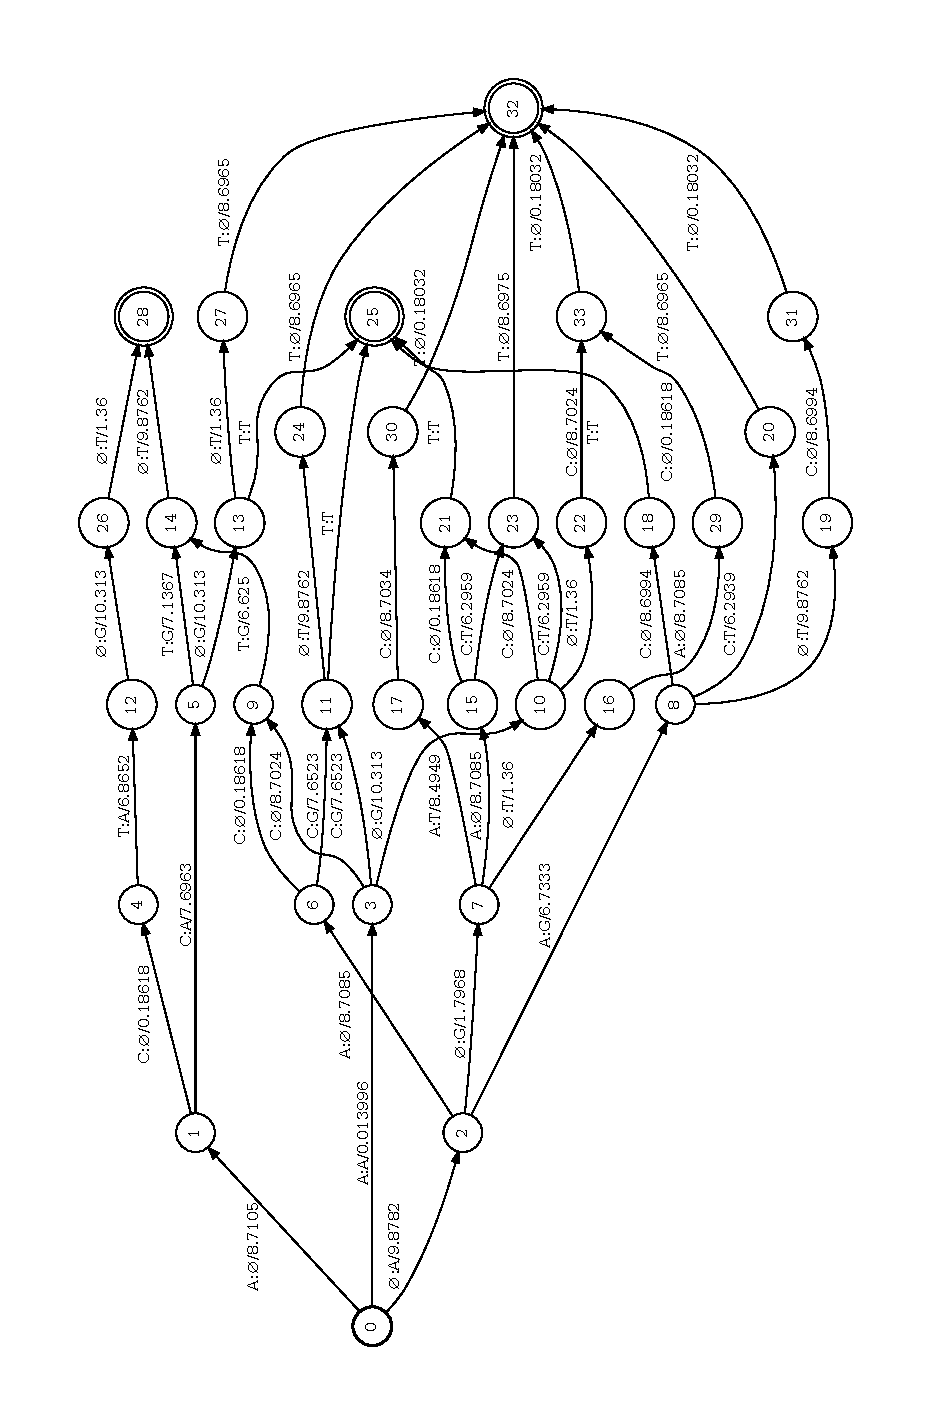
\includegraphics[width=\textheight,height=0.65\textwidth,keepaspectratio,angle=-90]{defense/figures/graph-fst.pdf}
\note[item]{$\oplus$: combination operator; $\otimes$: aggregation operator.}
\end{frame} %-------------------------------------------------------------------

\begin{frame}[t,noframenumbering]{FST Alignment} %-------------------------------
\begin{itemize}
    \item Contains all possible alignments: ancestor sequence transducer $\times$ Evolution FST $\times$ descendant sequence transducer.
    \item The best alignment is the highest probability path from start to end state, found using the Viterbi algorithm.
\end{itemize}
\centering
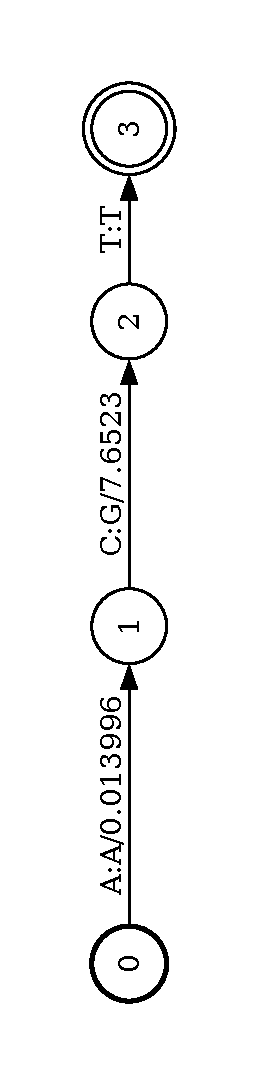
\includegraphics[width=\textheight,height=0.8\textwidth,keepaspectratio,angle=-90]{defense/figures/path-fst.pdf}
\note[item]{FST operations, including this graph, are made using the openFST library.}
\end{frame} %-------------------------------------------------------------------

\begin{frame}[t,noframenumbering]{FST Alignment} %-------------------------------
\begin{itemize}
    \item Contains all possible alignments: ancestor sequence transducer $\times$ Evolution FST $\times$ descendant sequence transducer.
    \item The best alignment is the highest probability path from start to end state, found using the Viterbi algorithm.
    \item The ancestor sequence is assumed of high quality to preserve the reading frame and safeguard against frameshifts in the potentially lower-quality descendant sequence.
    \item openFST library supports multiple semirings, we use tropical.
    % \item FST operations are done using the tropical semiring and openFST library.
\end{itemize}
% \vspace{1em}
\centering
\begingroup\centering
\begin{tabular}{c||c|c|c|c|c}
Semiring & Set & $\oplus$ & $\otimes$ & $\overline{0}$ & $\overline{1}$\\
\hline\hline
Linear   & $ \mathbb{R}$ & $+$ & $\times$ & $0$ & $1$\\
Log      & $ \mathbb{R} \cup \{ -\infty, +\infty \}$ & $\oplus_{\log}$ & $+$ & -$\infty$ & 0\\
Tropical & $ \mathbb{R} \cup \{ -\infty, +\infty \}$ & $\max$ & $+$ & -$\infty$ & 0\\
\end{tabular}
\par\endgroup
\note[item]{Explain table.}
\note[item]{$\oplus$: combination operator; $\otimes$: aggregation operator.}
\end{frame} %-------------------------------------------------------------------

\begin{frame}{Methods} %--------------------------------------------------------
% \TODO{Rethink pipeline figure. Sequence examples??}
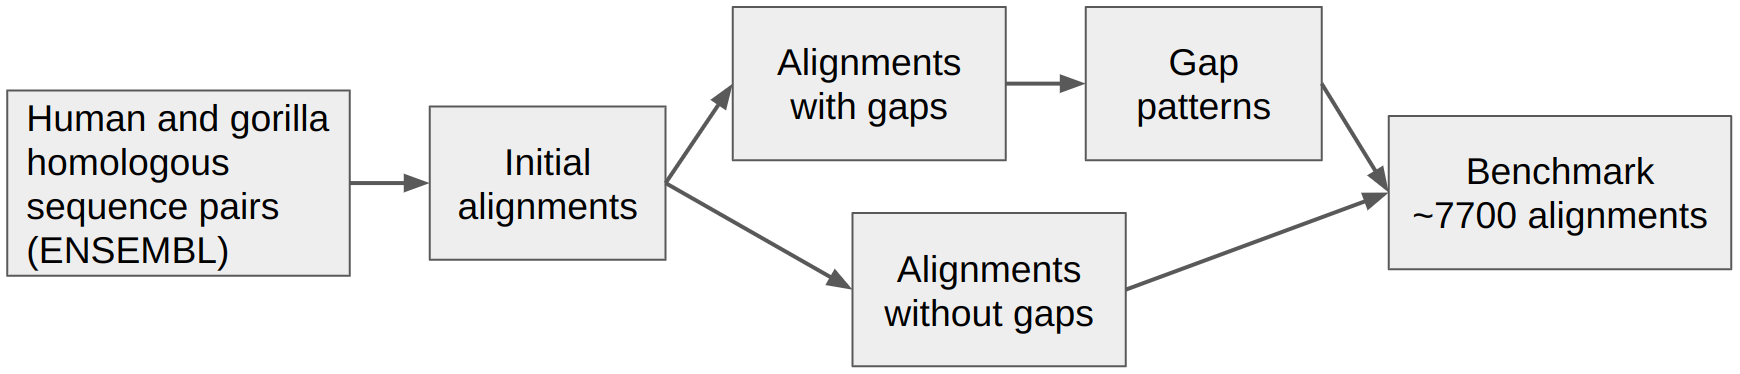
\includegraphics[width=0.95\textwidth]{images/fig-pipeline.png}
\vspace{1em}
\begin{columns}[b]
    \hspace{1cm}
    \column{0.3\textwidth}
    \textbf{Aligners:}\\
    \begin{itemize}
        \item COATi: Codon model
        \item MAFFT: DNA model
        \item PRANK: Codon model
    \end{itemize}
    \column{0.7\textwidth}
    % Metrics:\\
    \begin{itemize}
        \item MACSE: Amino acid model + frameshifts
        \item Clustal $\Omega$: Amino acid model
        % \item Avg alignment error ($d_{seq}$)
        % \item Number of perfect alignments
        % \item Accuracy of selection ($\text{F}_1$ score using $K_a K_s$)
    \end{itemize}
\end{columns}
\note[item]{To test the accuracy of COATi we generated a benchmark of pairwise alignments and tested it against (aligners).}
\note[item]{To generate the data set, we downloaded all the available human and gorilla homologous sequence pairs from ensembl (~16000).}
\note[item]{And we aligned all of them using all 5 methods (initial alignments).
Then we divided them into alignments that had gaps and alns that did not have any gaps.}
\note[item]{To generate the final data set, we introduced the gap patterns extracted from the first group into the gapless ones.}
\end{frame} %-------------------------------------------------------------------

\begin{frame}{Metrics} %--------------------------------------------------------
\begin{itemize}
    \setlength\itemsep{1em}
    \item Distance between alignments $d_{seq}$
        \begin{itemize}
            \setlength\itemsep{1em}
            \item Takes into account indels, symmetric, values in range $[0,1]$
            % \item Symmetric %(d(A,B) = d(B,A))
            % \item Values in range $[0, 1]$
        \end{itemize}
    \item Number of perfect and imperfect alignments
        \begin{itemize}
            \setlength\itemsep{1em}
            \item Perfect: $d_{seq} = 0$ or equivalent alignment
            \item Imperfect: not perfect when at least one method found perfect
        \end{itemize}
    \item Kimura two-parameter evolutionary distance between alignments.
    \item Accuracy of selection (using $k_a$ and $k_s$)
        \begin{itemize}
            \setlength\itemsep{1em}
            \item $k_a$: \# of substitutions per non-synonymous site
            \item $k_s$: \# of substitutions per synonymous site
            \item False discovery rate: 1 - precision = $\frac{FP}{FP+TP}$
            \item False negative rate: 1 - recall = $\frac{FN}{FN+TP}$
            % \item F$_1$: harmonic mean of precision and recall $\frac{2 \text{TP}}{2 \text{TP} + \text{FP} + \text{FN}}$
        \end{itemize}
\end{itemize}
\note[item]{To evaluate the performance of each method, we used the avg alignment error or distance metric dseq, the number of perfect and imperfect alignments, evolutionary distance between alns, and accuracy of identifying events of pos and neg selection using $k_a$ and $k_s$ (reported using FDR and FNR).}
\note[item]{FDR: proportion of false positives. FNR: proportion of missed positives (false negatives).}
\note[item]{$k_a$: no changes at the amino acid level}
\note[item]{$k_s$: introduces changes at the amino acid level}
\end{frame} %-------------------------------------------------------------------

\begin{frame}{Results} %--------------------------------------------------------
% \cyan{Plots for results?}
\centering{\scalebox{0.9}{% \begin{table}[h!]
% \begin{adjustbox}{width=\columnwidth,center}
\definecolor{bestcolor}{RGB}{230,230,230}

\begingroup\centering
\begin{tabular}{r|ccccc}
      & \textbf{COATi} & \textbf{MAFFT} & \textbf{PRANK\textsuperscript{*}} & \textbf{MACSE} & \textbf{Clustal$\Omega$}\\
\hline
Method    & Trip-MG & DNA & Codon & DNA+AA & AA\\[2pt]
%\hline
Avg alignment error ($d_{seq}$) & \cellcolor{bestcolor}0.00221 & 0.01471 & 0.01828 & 0.01399 & 0.02929\\
Perfect alignments & \cellcolor{bestcolor}5139 & 4692 & 4774 & 3737 & 2615\\
Imperfect alignments & \cellcolor{bestcolor}1048 & 1549 & 2116 & 3980 & 3948\\
% \hline
% F1 score for positive selection & \cellcolor{bestcolor}98.1\pct & 84.3\pct & 86.7\pct & 79.5\pct & 68.7\pct \\
% F1 score for negative selection & \cellcolor{bestcolor}99.8\pct & 98.4\pct & 98.7\pct & 98.2\pct & 96.9\pct \\
K2P distance RMSE & \cellcolor{bestcolor}0.0005 & 0.035 & 0.037 & 0.032 & 0.052 \\
Overestimated K2P distance & \cellcolor{bestcolor}10.9\pct & 26.6\pct & 33.8\pct & 48.7\pct & 61.8\pct \\
FDR positive selection & \cellcolor{bestcolor}2.6\pct & 17.6\pct & 12.8\pct & 10.3\pct & 30.8\pct \\
FNR positive selection & \cellcolor{bestcolor}1.3\pct & 13.6\pct & 13.7\pct & 28.7\pct & 31.9\pct \\
FDR negative selection & \cellcolor{bestcolor}0.1\pct & 1.4\pct & 1.4\pct & 2.8\pct & 3.1\pct \\
FNR negative selection & \cellcolor{bestcolor}0.3\pct & 1.8\pct & 1.3\pct & 0.8\pct & 3\pct \\
% FDR positive selection & \cellcolor{bestcolor}0.026 & 0.176 & 0.128 & 0.103 & 0.308 \\
% FNR positive selection & \cellcolor{bestcolor}0.013 & 0.136 & 0.137 & 0.287 & 0.319 \\
% FDR negative selection & \cellcolor{bestcolor}0.001 & 0.014 & 0.014 & 0.028 & 0.031 \\
% FNR negative selection & \cellcolor{bestcolor}0.003 & 0.018 & 0.013 & 0.008 & 0.030 \\
%
%          FDR.pos FNR.pos FDR.neg FNR.neg
% tri-mg     0.026   0.013   0.001   0.003
% mafft      0.176   0.136   0.014   0.018
% prank      0.128   0.137   0.014   0.013
% macse      0.103   0.287   0.028   0.008
% clustalo   0.308   0.319   0.031   0.030
%
\hline
\multicolumn{6}{c}{\rule{0pt}{1em}\textit{*} PRANK produced 42 empty alignments.}
\end{tabular}
\par\endgroup
% \end{adjustbox}
% \end{table}
% Best alignments & \cellcolor{bestcolor}5152 & 4833 & 4748 & 3754 & 2595\\
}}
\vspace{1em}
% \begin{itemize}
% 	\item AA-based aligners have difficulties retrieving
% 		positive selection.
% 	\item PRANK (no frameshifts) together with CLUSTAL$\Omega$ have the highest
% 		alignment error.
% 	\item MAFFT and MACSE (AA-based and frameshifts) have lower
% 		alignment error but also have difficulties with positive selection.
% \end{itemize}
% Pinpoint shortcomings of aligners
\note[item]{1st row: distance metric, the lower the better.}
\note[item]{Clustal$\Omega$ has difficulty "recovering/maintaining" positive
selection given its AA-based alignment.}
\note[item]{PRANK fails to align sequences with incomplete codons (length not multiple of three).}
\end{frame} %-------------------------------------------------------------------

\begin{frame}[c]{Average Distance Between Alignments---$d_{seq}$} %-------------
\centering
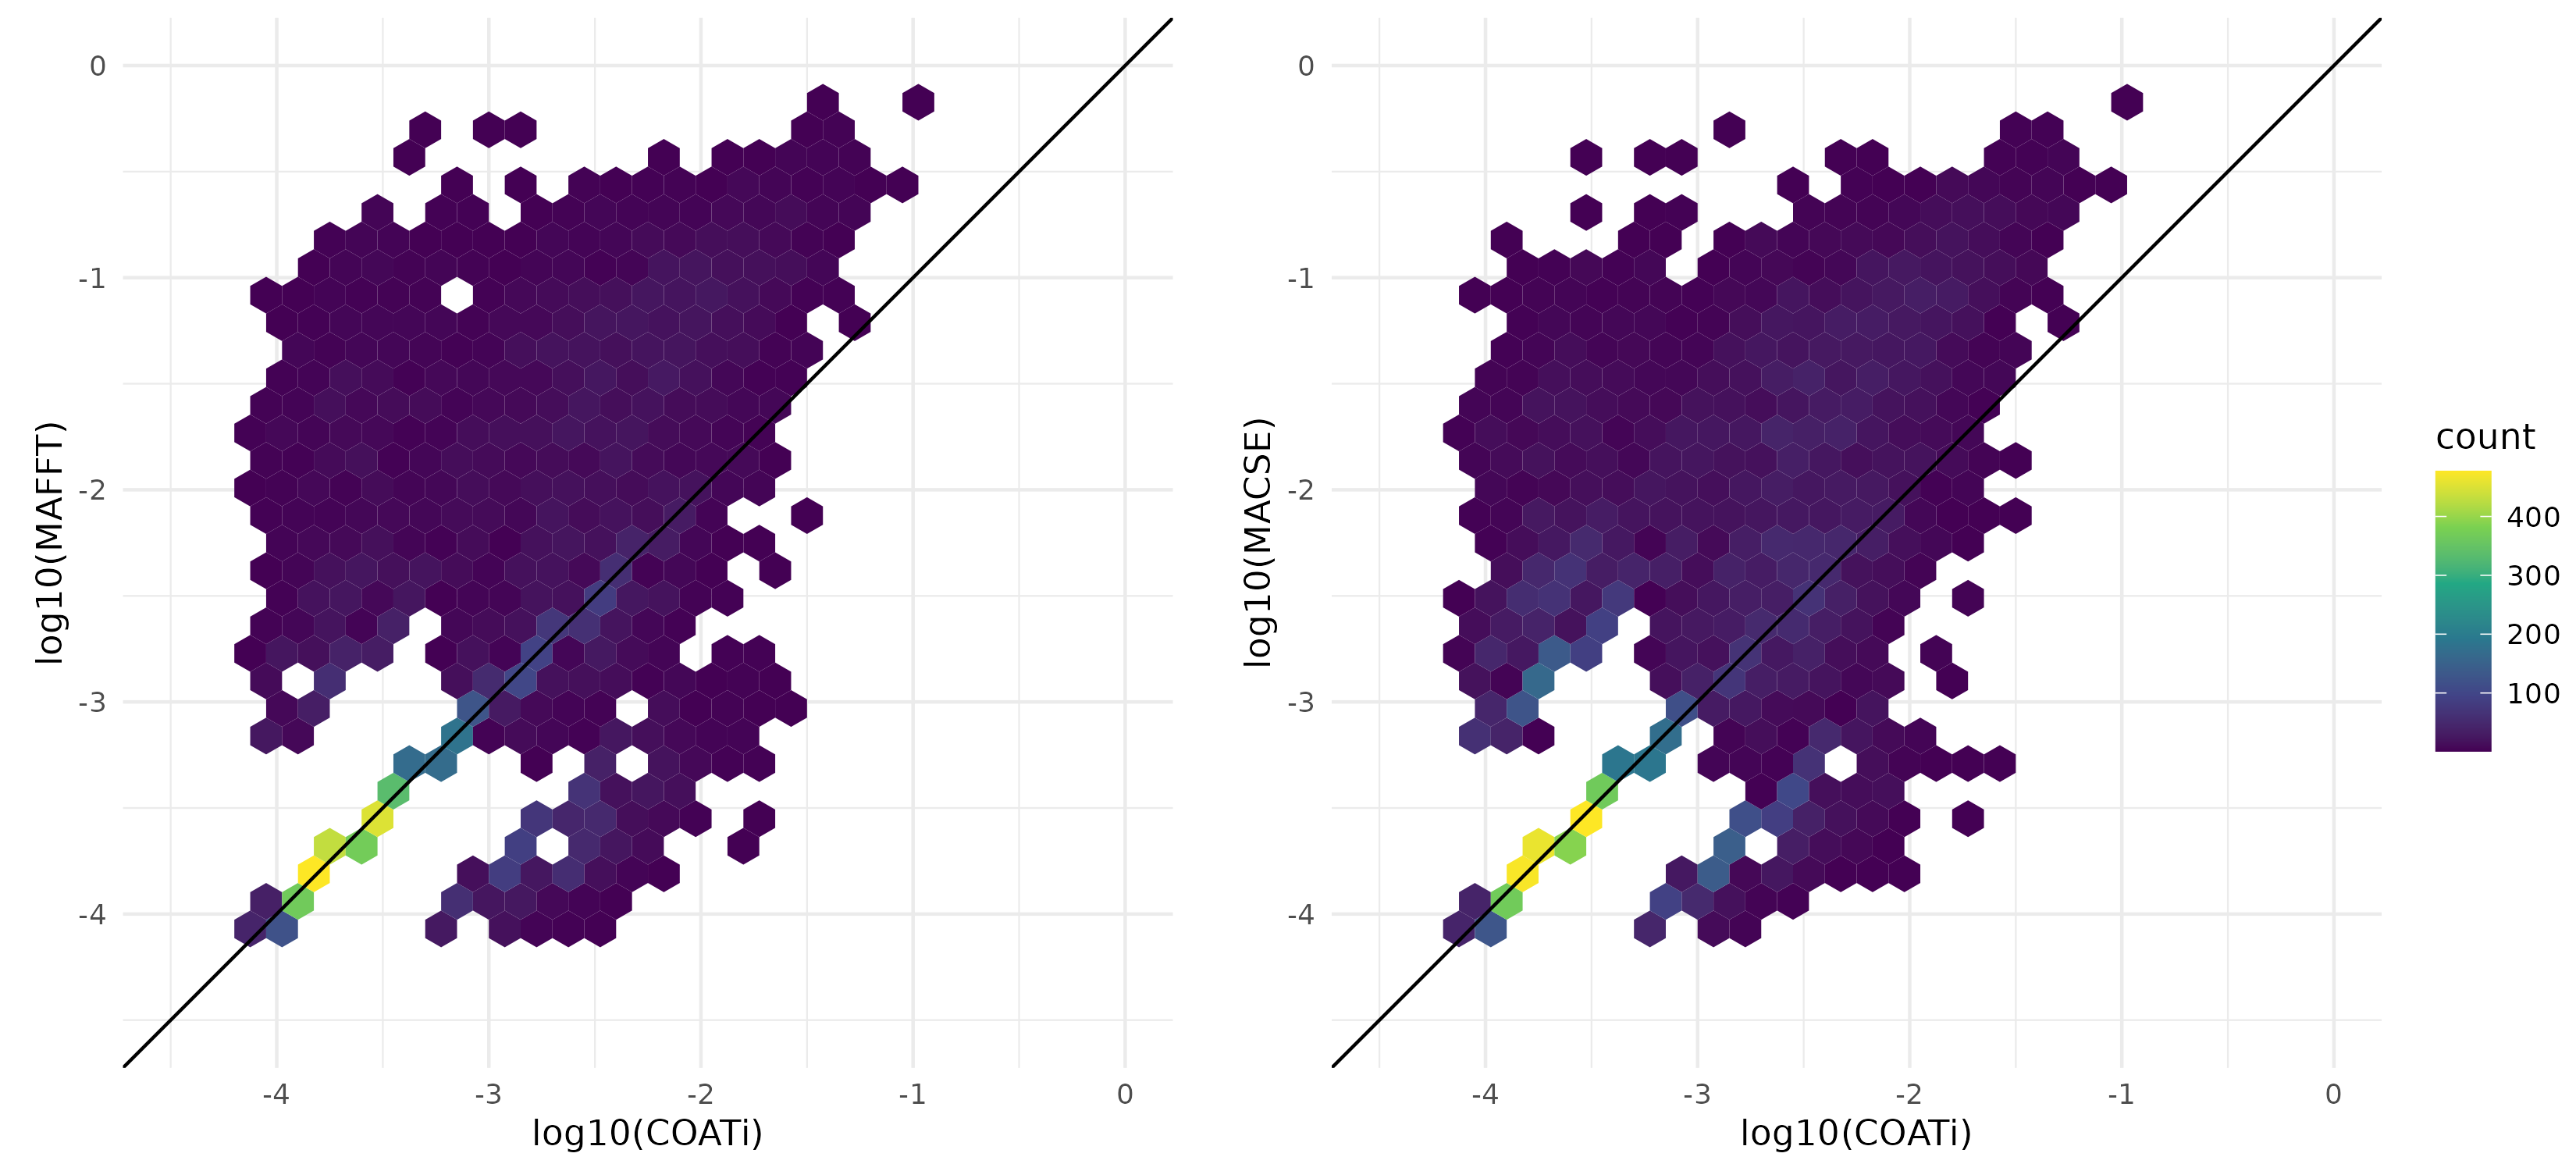
\includegraphics[width = \textwidth]{defense/images/dseq_plots_mafft_macse_tri-mg.png}
\end{frame} %-------------------------------------------------------------------

\begin{frame}[c]{Average Distance Between Alignments---$d_{seq}$} %-------------
\centering
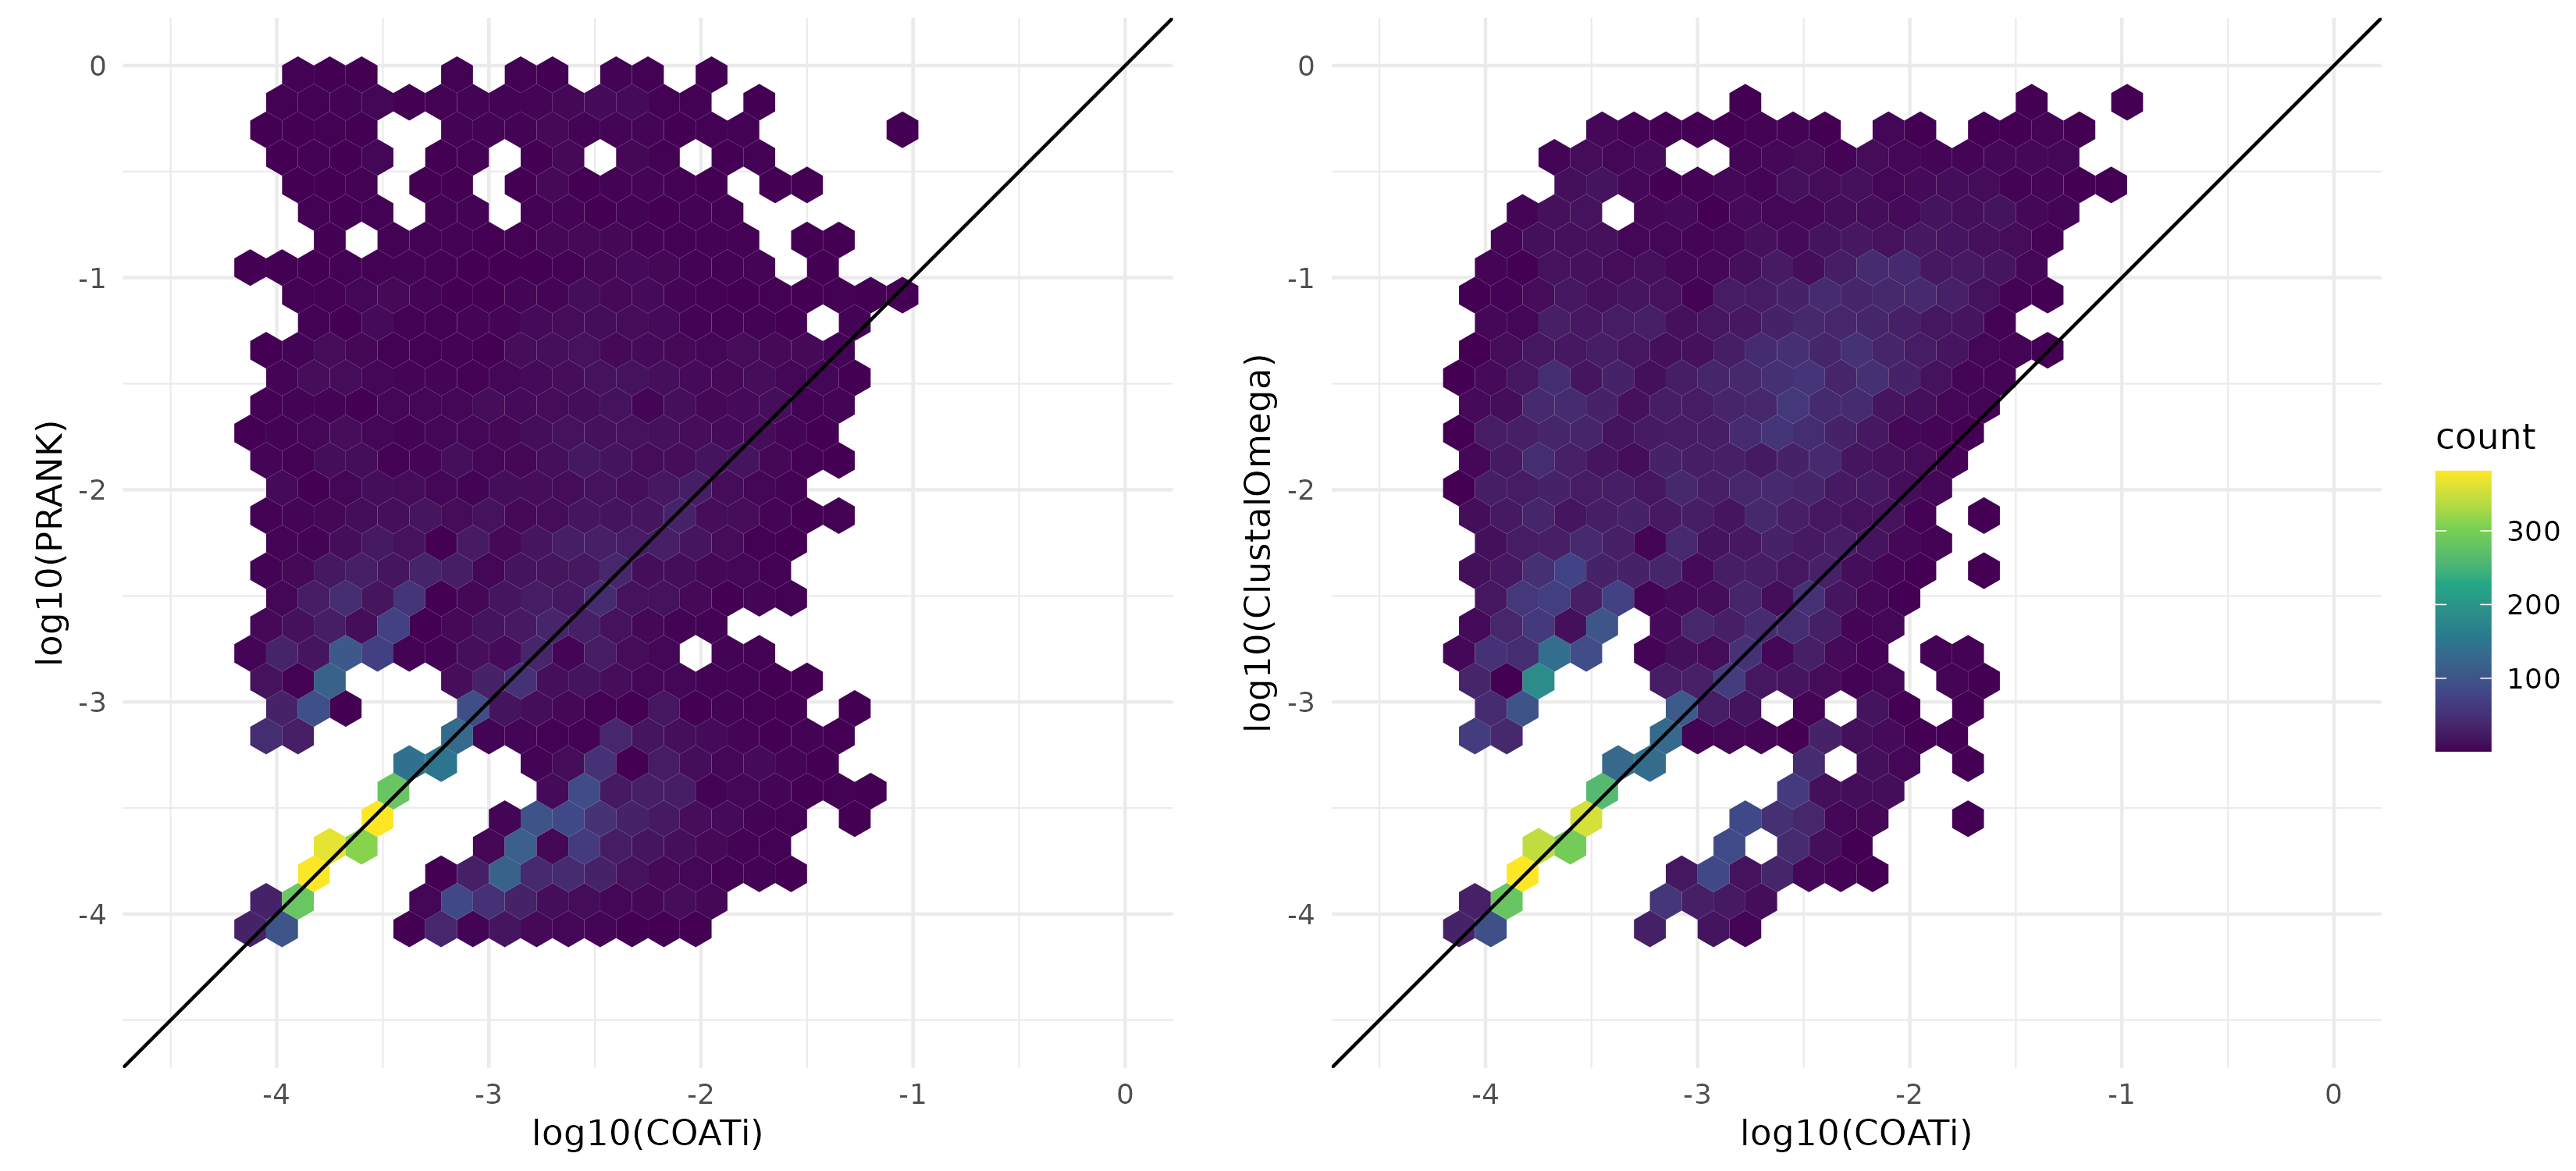
\includegraphics[width = \textwidth]{defense/images/dseq_plots_prank_clustalo_tri-mg.png}
\end{frame} %-------------------------------------------------------------------

% \begin{frame}{Results} %--------------------------------------------------------
% Using gorillas as the ancestor, I aligned the benchmark alignments without an early stop codon in the simulated gorilla sequence (4003/7751).\\

% \vspace*{2em}\scalebox{0.9}{\definecolor{bestcolor}{RGB}{230,230,230}

\begingroup\centering
\begin{tabular}{r|cccccc}
      & \textbf{COATi} & \textbf{MAFFT} & \textbf{PRANK} & \textbf{MACSE} & \textbf{Clustal$\Omega$} & \textbf{COATi-rev}\\
\hline
Method    & Marg-MG & DNA & Codon & DNA+AA & AA & Marg-MG\\[2pt]
%\hline
Avg alignment error ($d_{seq}$) & \cellcolor{bestcolor}0.00113 & 0.00586 & 0.00358 & 0.00448 & 0.02099 & 0.00118\\
Perfect alignments & \cellcolor{bestcolor}3501 & 3162 & 2829 & 2552 & 1772 & 3463\\
Imperfect alignments & \cellcolor{bestcolor}309 & 648 & 981 & 1258 & 2038 & 347\\
% \hline
F1 score for positive selection & \cellcolor{bestcolor}99.3\pct & 91.1\pct & 90.3\pct & 87.2\pct & 76.0\pct & 99.0\pct \\
F1 score for negative selection & \cellcolor{bestcolor}99.9\pct & 99.1\pct & 99.1 & 98.9\pct & 97.7\pct & 99.9\pct \\
\end{tabular}
\par\endgroup

}
% % \vspace{1em}
% % \TODO{By origin results}\\
% % \TODO{Reverse pipeline results?}
% \end{frame} %-------------------------------------------------------------------

% \begin{frame}{COATi in action} %------------------------------------------------
% Comment on the results of the 2nd author manuscript from the lab where COATi was used
% to analyze indel patterns in CDSs.
% \end{frame} %-------------------------------------------------------------------

\begin{frame}[b]{Biological Application} %-------------------------------------------
\centering
\shadowbox{%
\adjincludegraphics[height=0.7\textheight,trim={0 {0.45\height} 0 0},clip=true,]{defense/figures/ziqi_diss.pdf}
}
\par
\begin{tikzpicture}[remember picture,overlay]
\draw node[anchor=south east,text width = 35mm,align=center,font=\footnotesize]
  at ($(current page.south east)+(-5mm,5mm)$)
  {\pgfimage[height=30mm]{defense/images/ziqi_zhu.jpg}\\
  Dr. Ziqi Zhu};

\end{tikzpicture}

%%%
\note[item]{In collaboration with Dr. Ziqi Zhu; he used COATi \& and helped me improve my models.}
\note[item]{Second author manuscript in process.}
\note[item]{Dataset: 90 different clades representing all three domains of life (Zou \& Yang 2019).}
\note[item]{Most likely alignment using \textbf{COATi}.}
\note[item]{Estimation of alignment parameters for each species-pair.}
\note[item]{Summarize alignments to understand indel phases.}
\end{frame} %---------------------------------------------------------------------

\begin{frame}[c]{Indel Model Parameters} %---------------------------------
\centering
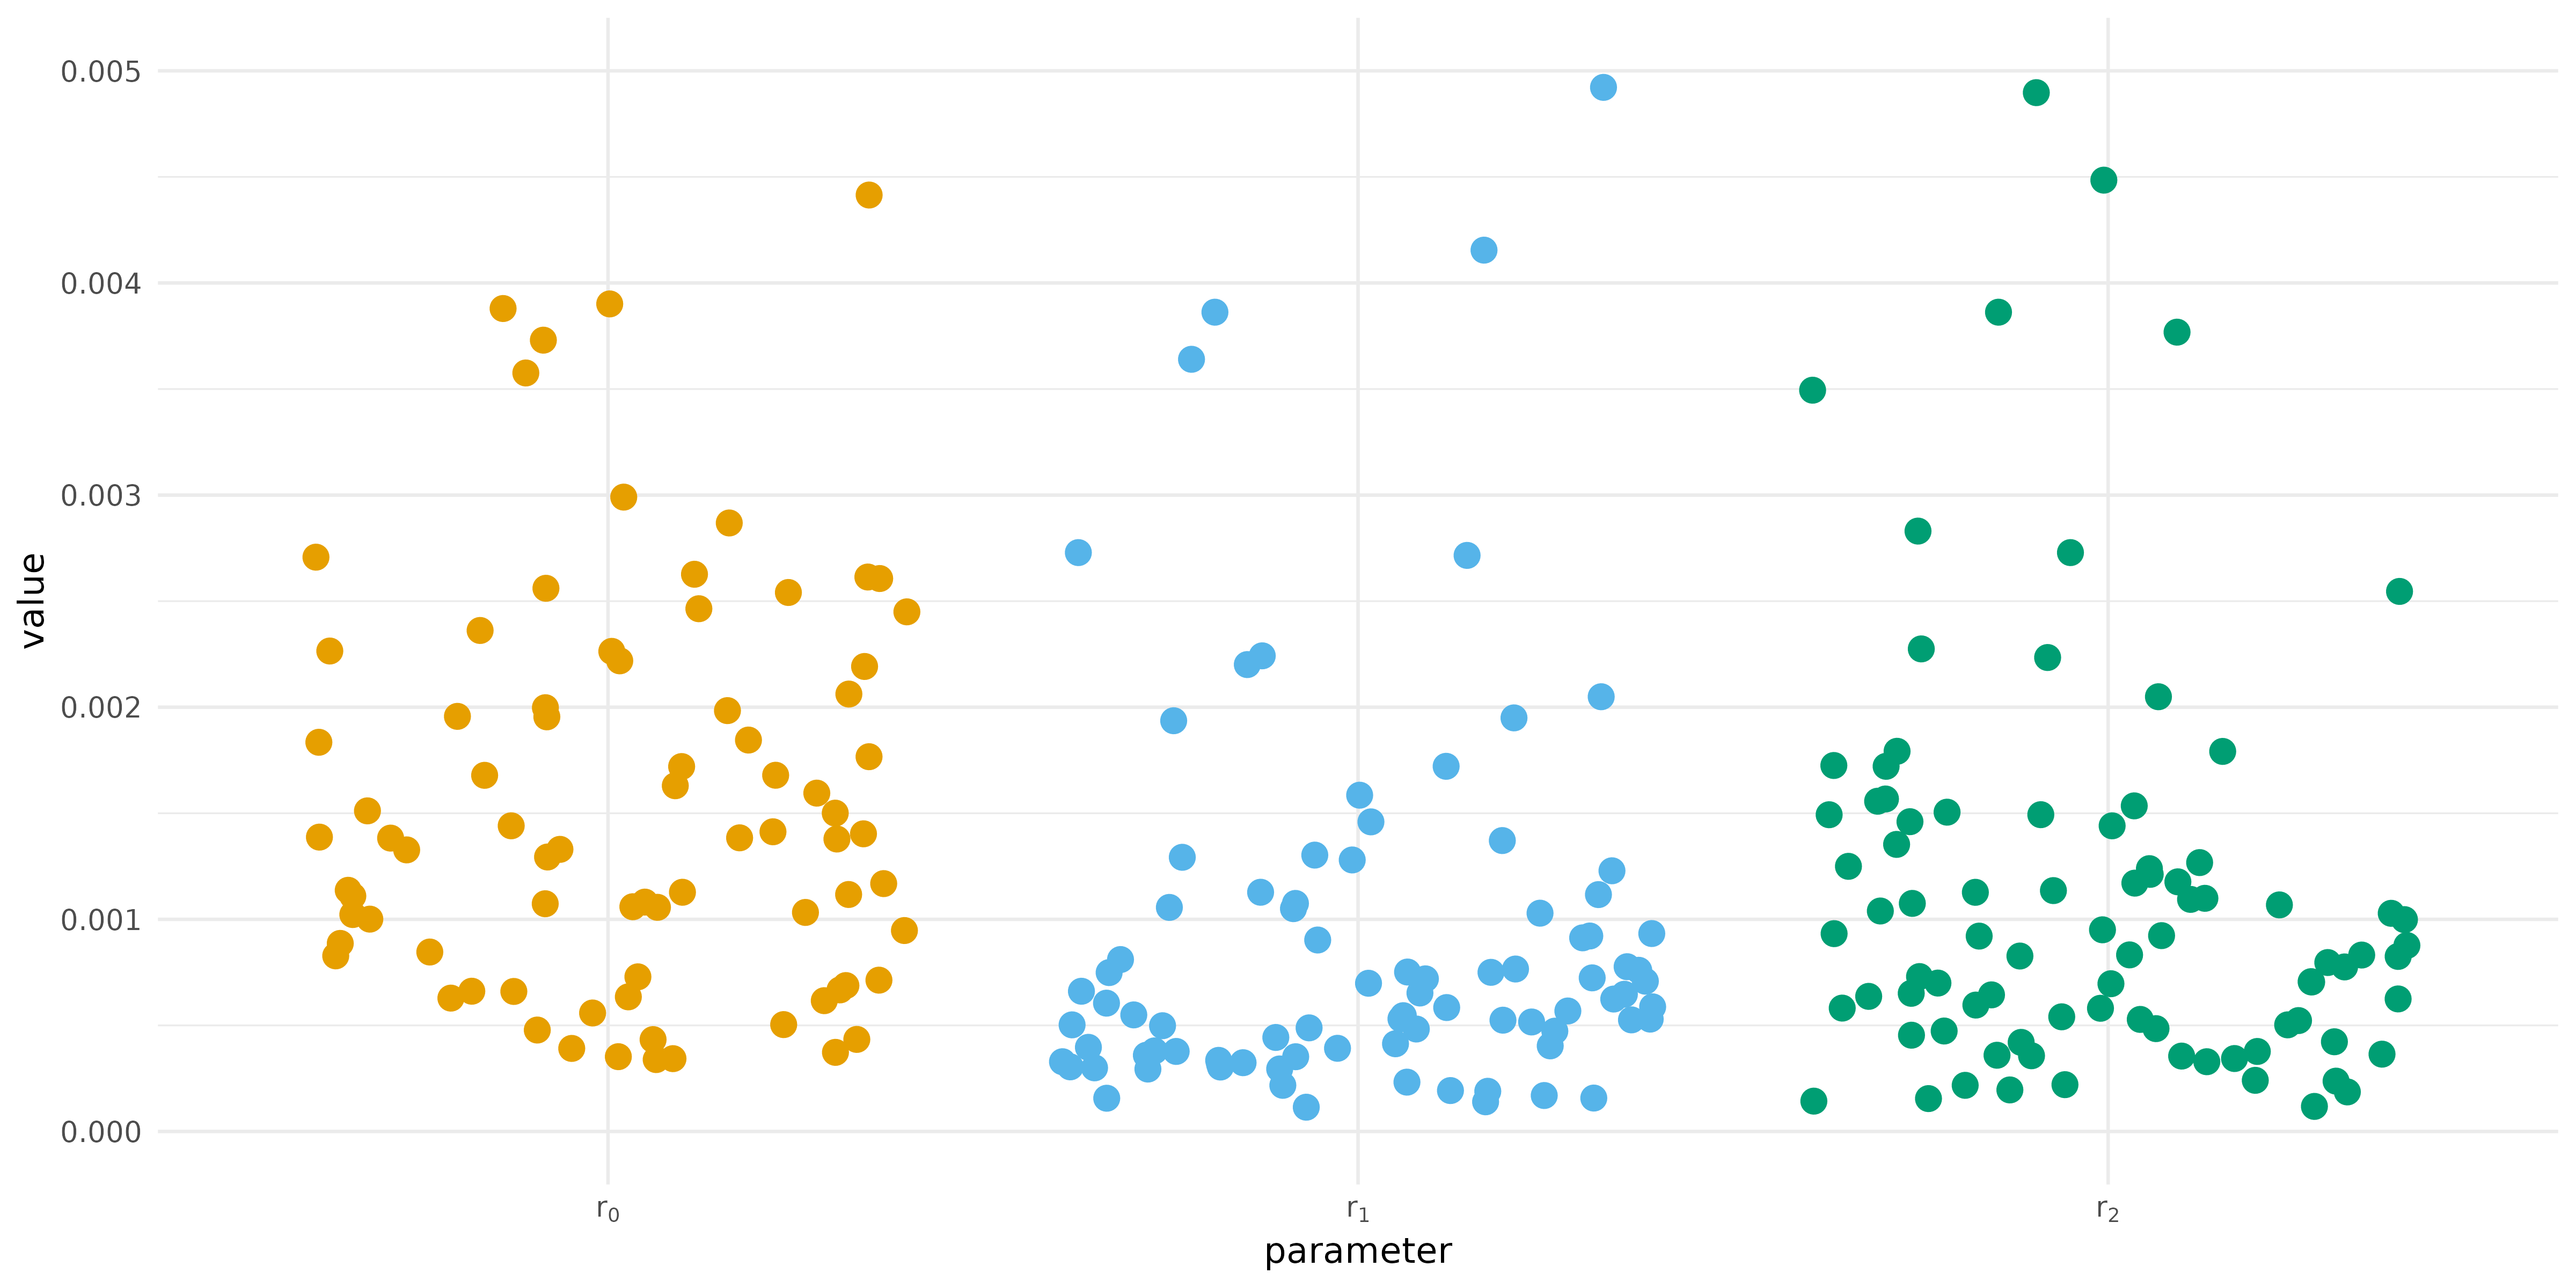
\includegraphics[height = 0.8\textheight]{defense/images/gap_90_species_estimates.png}
\note[item]{Parameters are estimates of the rate of indels per branch length if $\omega$ = 1.}
\note[item]{The trend is that r0 is larger than r2 which in turn is larger than r1. Because its paired data, <next slide>.}
\end{frame} %-------------------------------------------------------------------

\begin{frame}[c]{Indel Model Parameters} %---------------------------------
\centering
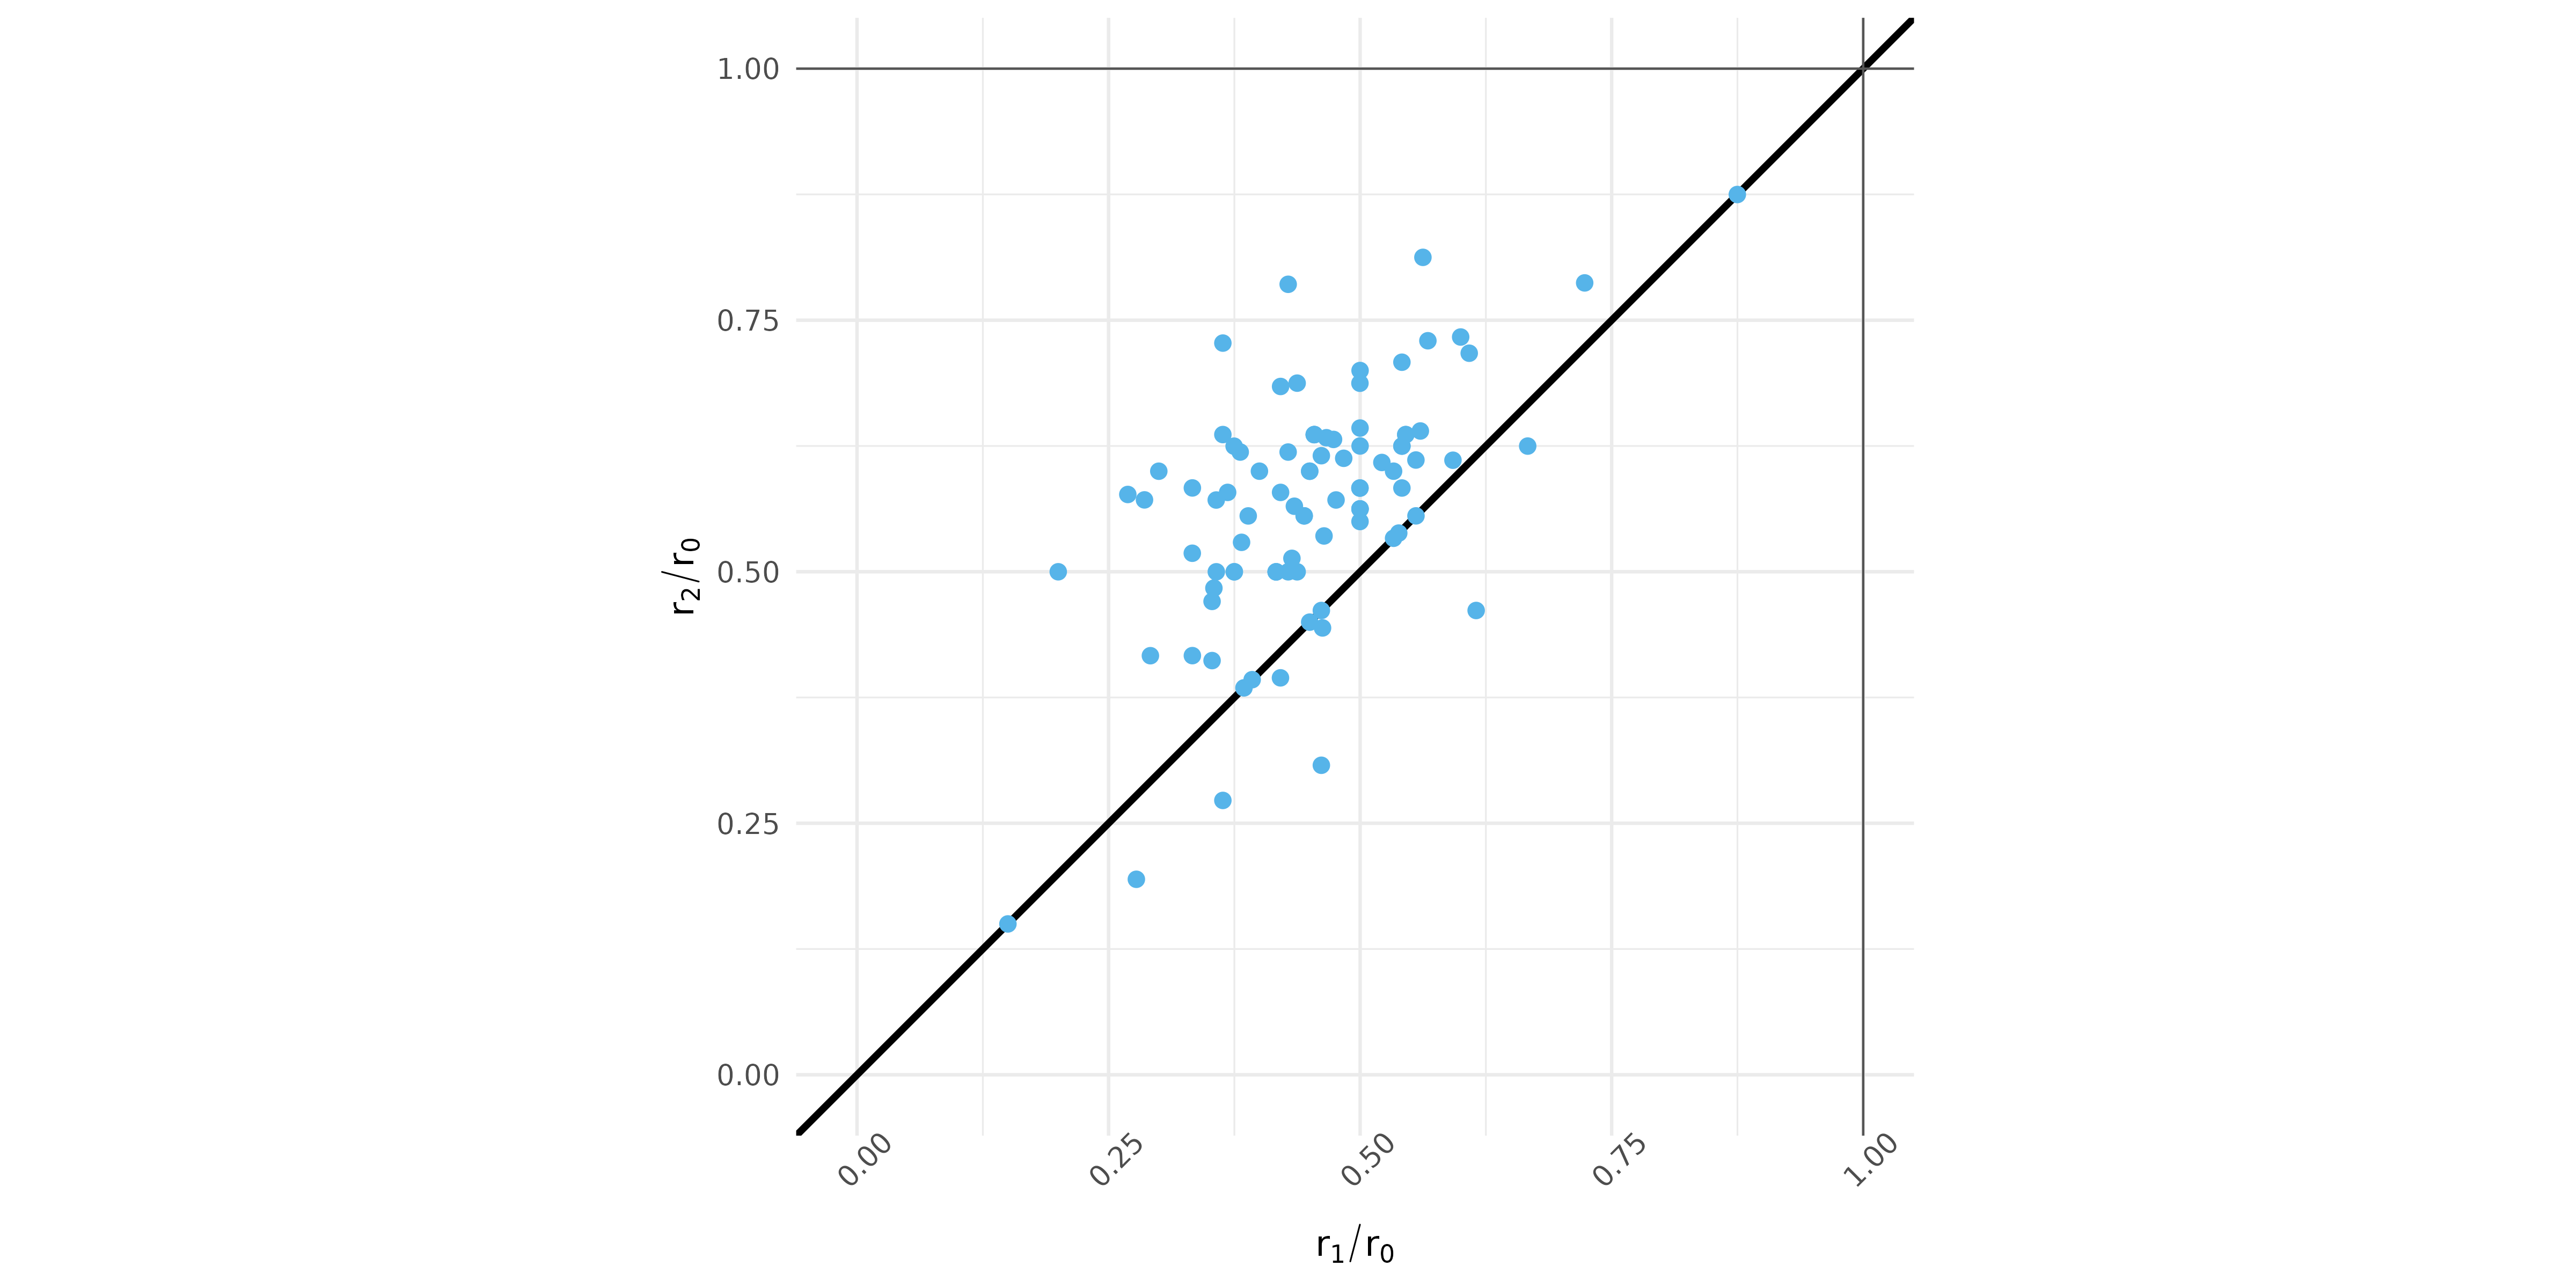
\includegraphics[height = 0.8\textheight]{defense/images/gap_90_species_relative.png}
\note[item]{We can compare the values directly. X-axis is r1/r0 and y-axis is r2/r0. Because all points are below 1 in both axis, r0 is always larger. The majority of points is above the abline, so in general r2 is larger than r1. Which makes sense for protein-coding regions, since we expect them to be under purifying selection.}
\end{frame} %-------------------------------------------------------------------

\begin{frame}[c]{Indel Phases Are Similar Across Species} %-----------------------
\centering
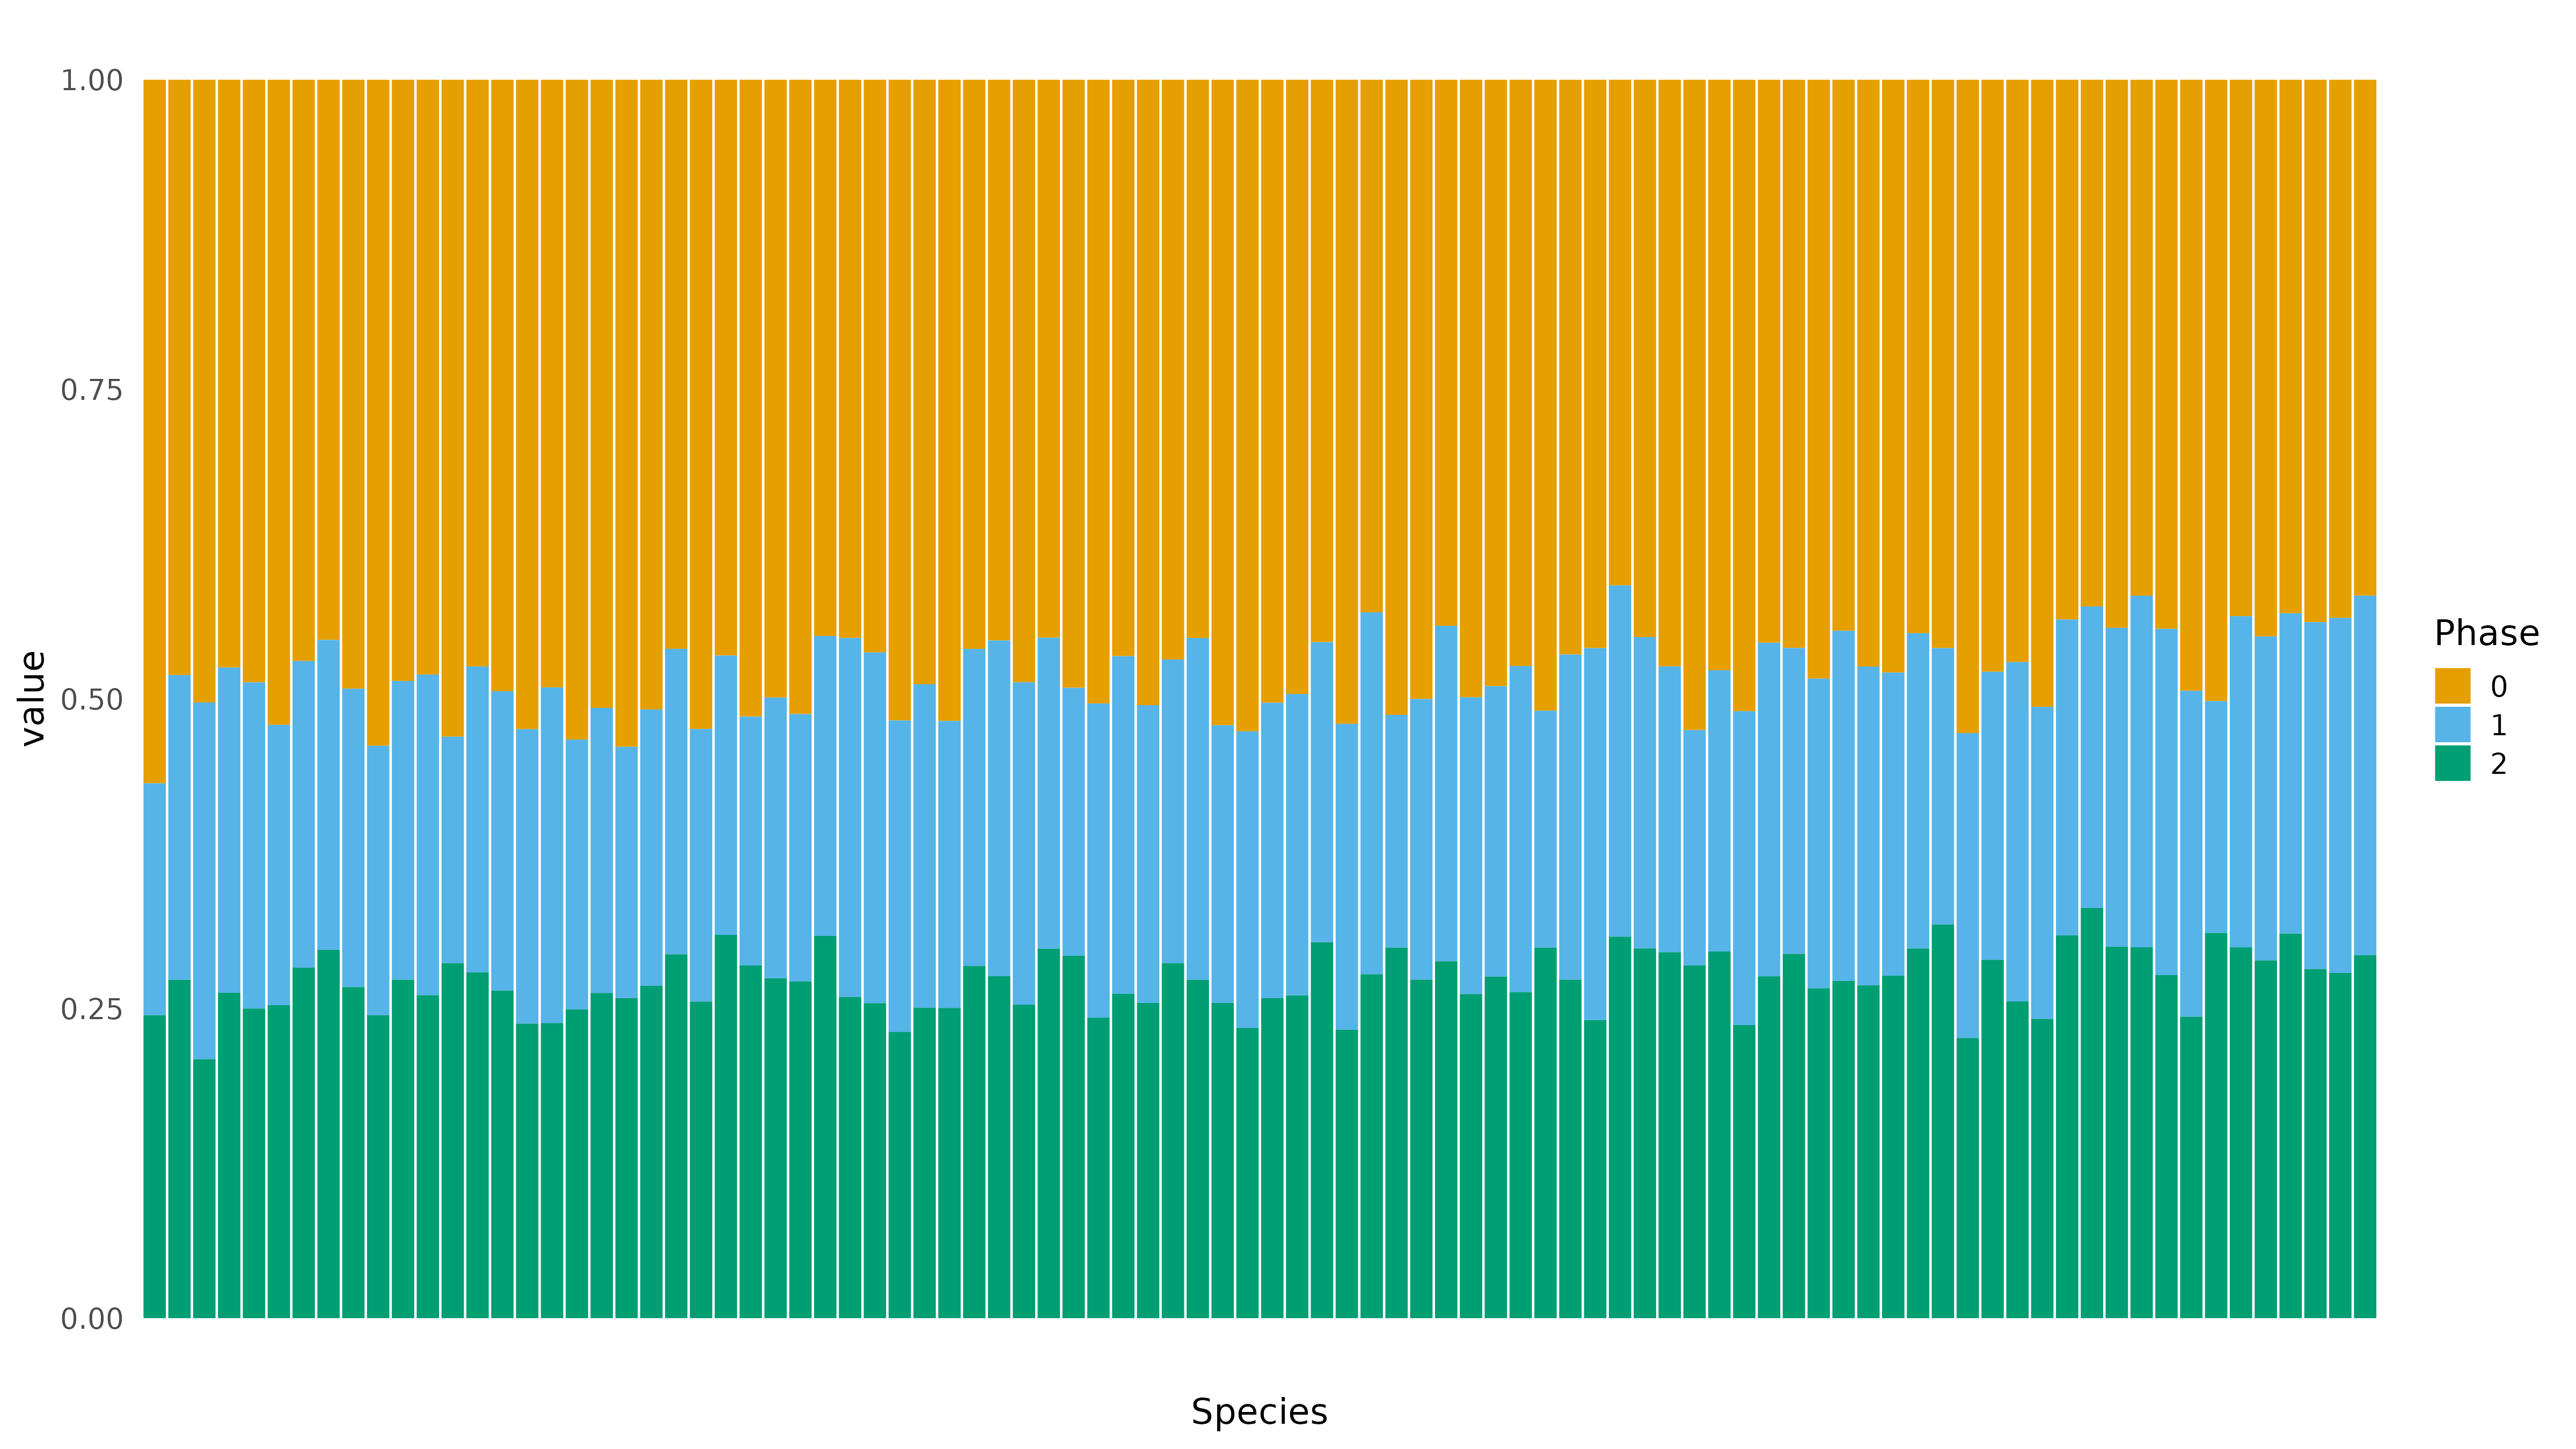
\includegraphics[height = 0.9\textheight]{defense/images/indel_phases_90_species.png}
\note[item]{If we take a look at the proportion of phase 0,1,2 gaps, we see that about 50\% of gaps are phase0. Aligners that only consider phase 0 gaps miss the optimal alignment about 50\% of the time.}
\end{frame} %-------------------------------------------------------------------

\begin{frame}[c]{Runtime} %-----------------------------------------------------
\centering
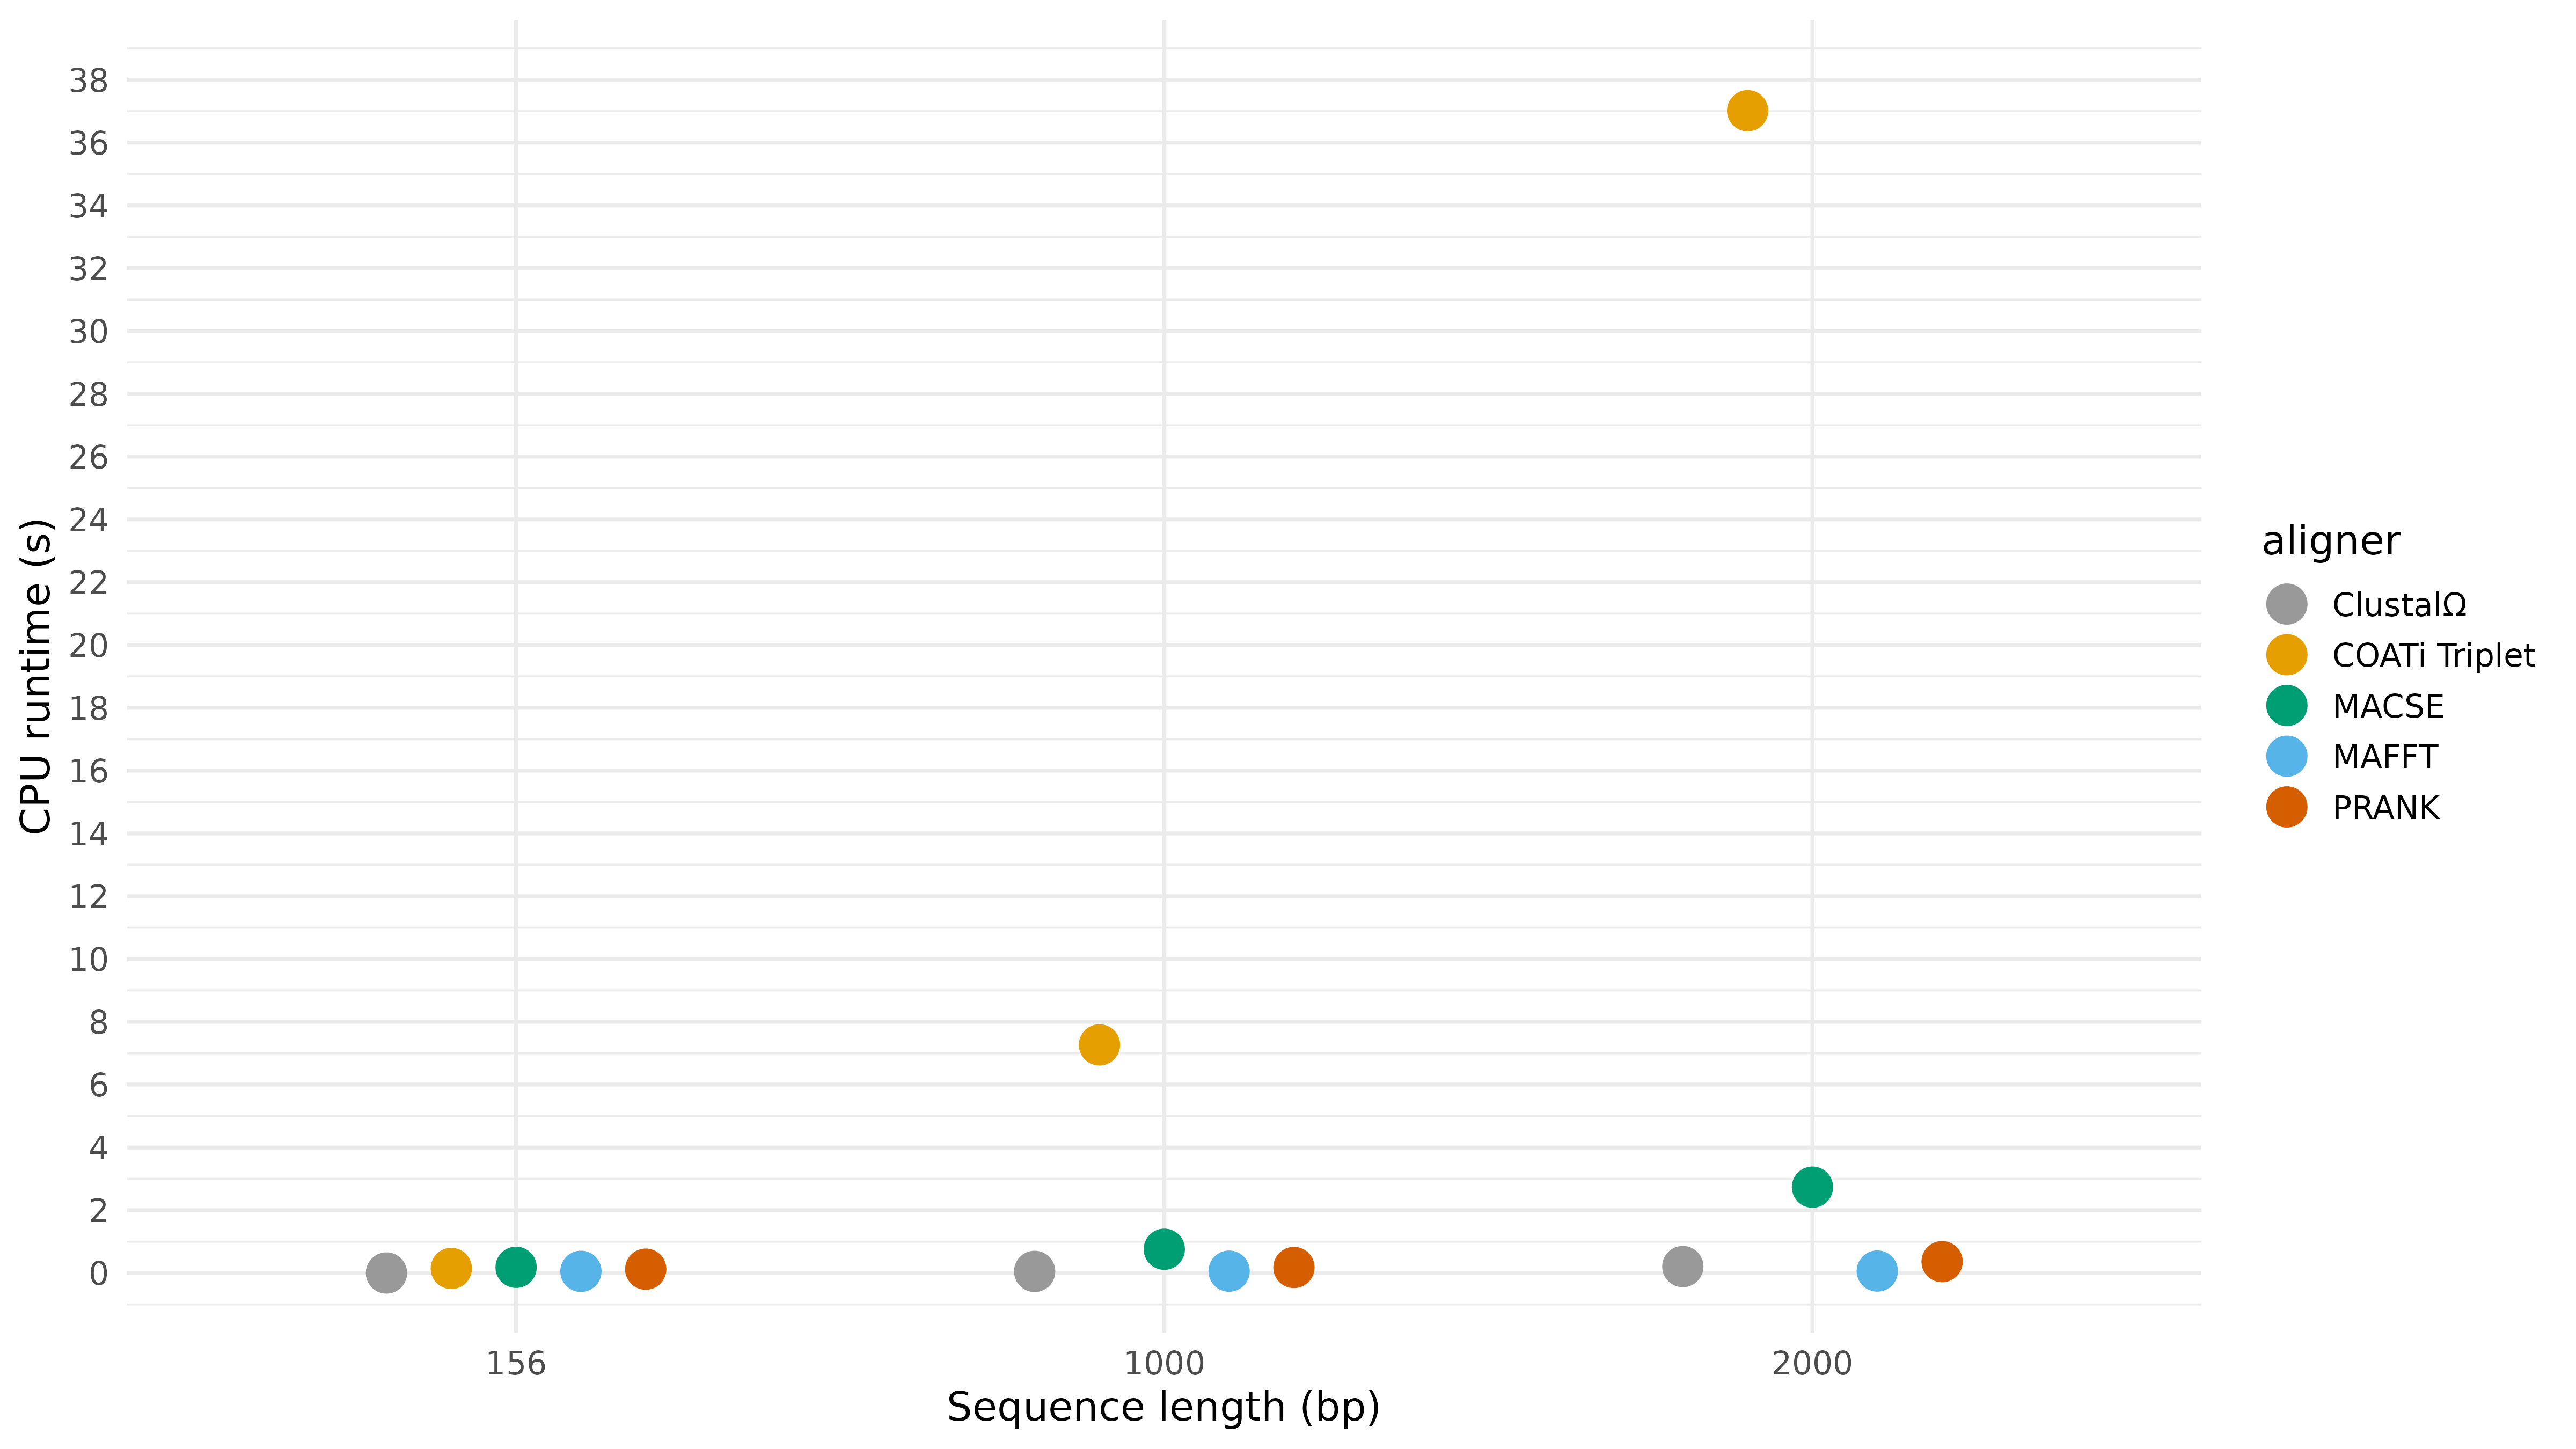
\includegraphics[height = 0.8\textheight]{defense/images/runtime_aligners_triplet.png}
\end{frame} %-------------------------------------------------------------------

%% AlnPlot: illustrate with an example that current options can't always distinguish between 2 alignments.

\begin{frame}[t]{Marginal Model} %----------------------------------------------
\begin{itemize}
    \setlength\itemsep{1em}
    \item<1-> \textbf{Limitation}: considering the space of all possible alignments consumes time and memory in FST-alignment.
    \item<2-> \textbf{Goal}: speed up alignment and reduce memory usage.
    \item<3> \textbf{Solution}
        \only<3>{\begin{itemize}
            \setlength\itemsep{1em}
            \item Adapt the evolution model to use in dynamic programming alignment.
            \item Marginal substitution model that approximates the triplet model.
            \item Output nucleotides are only dependent on the input codon and position.
        \end{itemize}}
\end{itemize}
\only<3>{%
\begin{table}
    \centering
    \begin{tabular}{lll}
          & States& Arcs\\
         \hline
         Evolution FST& 924 & 25,000\\
         Marginal model FST& 5 & 2,220\\
    \end{tabular}
\end{table}
}
\end{frame} %-------------------------------------------------------------------

\begin{frame}{Marginal Substitution Model} %------------------------------------
\begin{itemize}
    \item Let $X= \{X_0 X_1 X_2\}$ and $Y = \{Y_0 Y_1 Y_2\}$ be non-stop codons
    % from $\grande{\Sigma}_{codon}$
    \item Probability that $X \rightarrow Y$ after time $t$ in the triplet model is $P\left(Y_0 Y_1 Y_2 \middle| X_0 X_1 X_2; \Theta \right)$
\end{itemize}

\begin{equation*}
P_\text{mar}\left(Y_p = y \middle| X_0 X_1 X_2;\theta \right) =
\bigoplus_{Y_0 Y_1 Y_2} I(Y_p = y) \otimes P\left(Y_0 Y_1 Y_2 \middle| X_0 X_1 X_2;\Theta \right)
\end{equation*}

\only<1>{%
\begin{align*}
    P_\text{mar}\left(Y_0 = \bm{A} \middle| AGC;\theta\right) =~&P(\bm{A}AA|AGC) \oplus P(\bm{A}AC|AGC) \oplus P(\bm{A}AG|AGC) \oplus \cdots \\
    &\cdots \oplus P(\bm{A}TG|AGC) \oplus P(\bm{A}TT|AGC)
\end{align*}
}

\only<2>{%
\begin{itemize}
    \item Two marginal models defined
    \begin{itemize}
            \setlength\itemsep{1em}
        \item Max model from using the tropical semiring
        \item Sum model from using the linear or the log semiring
    \end{itemize}
\end{itemize}
}
\note[item]{$\oplus$ aggregation operator; $\otimes$ combination operator.}
\end{frame} %-------------------------------------------------------------------

\begin{frame}{Marginal Model} %-------------------------------------------------
\centering
\resizebox{!}{0.9\textheight}{
%\documentclass{article}
% \documentclass[tikz]{standalone}

% \usepackage{pgf}
% \usepackage{tikz}
% \usetikzlibrary{arrows,automata,positioning}
% %\usepackage[latin1]{inputenc}
% \usepackage{verbatim}
% \usepackage{graphicx}

% \usetikzlibrary{shapes,arrows,positioning}
% \tikzset{
%   font={\fontsize{9pt}{11}\selectfont}
% }

\definecolor{colorR}{RGB}{228,26,28}    % RED
\definecolor{colorB}{RGB}{55,126,184}   % BLUE
\definecolor{colorG}{RGB}{77,175,74}    % GREEN
\definecolor{colorP}{RGB}{152,78,163}   % PURPLE
\definecolor{colorO}{RGB}{255,127,0}    % ORANGE
\definecolor{colorY}{RGB}{255,255,51}   % YELLOW
\definecolor{colorBn}{RGB}{166,86,40}   % BROWN
\definecolor{colorPk}{RGB}{247,129,191} % PINK
\definecolor{colorGy}{RGB}{153,153,153} % GRAY

% \begin{document}

\begin{tikzpicture}[->,>=stealth',shorten >=1pt,auto,node distance=6cm,ultra thick]
  \tikzstyle{every node}=[font=\large]

  \node[circle,fill=colorG!50,minimum size=1cm]  (S)					  {\textbf{Start}};
  \node[circle,fill=colorB!50,minimum size=1cm]	 (M) [right=20mm of S]  {\textbf{M}};
  \node[circle,fill=colorB!50,minimum size=1cm]  (I) [above right of=M] {\textbf{I}};
  \node[circle,fill=colorR!50,minimum size=1cm]  (E) [below right of=M] {\textbf{End}};
  \node[circle,fill=colorB!50,minimum size=1cm]  (D) [below right of=I] {\textbf{D}};

  \path (S) edge 			  node {}	(M)
  		(M) edge [out=265,in=200,looseness=10]  node [midway,font=\large] {x$_\text{i}$:z$_\text{j}$ /$(1-\text{g})^2\cdot $s} (M)
  			edge [bend left]  node [font=\large] {\O:z$_\text{j}$/g} (I)
            edge         node [font=\large] {x$_\text{i}$:\O/ $(1-\text{g})\cdot$ g} (D)
            edge [bend right] node [font=\large] {$(1-\text{g})^2$}	(E)
        (I) edge [out=120,in=60,looseness=10] node [font=\large] {\O:z$_\text{j}$/ e} (I)
            edge [bend left]  node [rotate=50, above=1em, font=\large] {x$_\text{i}$:z$_\text{j}$/ $(1-\text{e})\cdot (1-\text{g}) \cdot$ s} (M)
            edge [bend left] node [font=\large] {x$_\text{i}$:\O/ $(1-\text{e}) \cdot$ g} (D)
            edge [bend left] node [pos=0.96, rotate=60, right=1.5em, font=\large] {$(1-\text{e}) \cdot (1-\text{g})$} (E)
        (D) edge [out=30,in=330,looseness=10] node [font=\large] {x$_\text{i}$:\O/ $e$} (D)
        	edge [bend left]  node [above=0.5em, font=\large] {x$_\text{i}$:z$_\text{j}$/ ($1-$e) $\cdot$ s} (M)
        	edge [bend left]  node [font=\large] {$1-$e} (E);

  \node[text width=4cm, below left=-8mm and 2cm of E] (parameters) {
  \begin{tabular}{r@{\,: }l}
  \multicolumn{2}{l}{\textbf{Parameters}}\\
    \hline
  g & gap opening\\
  e & gap extension\\
  s & substitution\\
  \end{tabular}
  };

  \node[text width=4cm, below right=-8mm and 3cm of E] (parameters) {
  \begin{tabular}{r@{\,: }l}
  \multicolumn{2}{l}{\textbf{Sequences}}\\
    \hline
  x & input sequence\\
  z & output sequence\\
  \O & empty sequence\\
  \end{tabular}
  };
\end{tikzpicture}

% \end{document}
}
\end{frame} %-------------------------------------------------------------------

\begin{frame}{Comparison of Marginal Models} %----------------------------------
\begin{itemize}
    \item Kullback-Leibler divergence between triplet and de-marginal models.
    \item Let $X= \{X_0 X_1 X_2\}$ and $Y = \{Y_0 Y_1 Y_2\}$ be non-stop codons
    % from $\grande{\Sigma}_{codon}$
    \item Probability that $X \rightarrow Y$ after time $t$ in the triplet model is $P\left(Y_0 Y_1 Y_2 \middle| X_0 X_1 X_2; \Theta \right)$
    \item Marginal to 61x61: $P_{de\text{-}mar}(Y|X) = P_{mar}(Y_0|X;\theta) \cdot P_{mar}(Y_1|X;\theta) \cdot P_{mar}(Y_2|X;\theta)$
\end{itemize}

\begin{equation*} \label{eq:KLD}
    D_{KL} (P | P_{de\text{-}mar}) = \sum_{x \in \chi} P(x) \log \left( \frac{P(x)}{P_{de\text{-}mar}(x)} \right)
\end{equation*}
\note[item]{To compare how well the marginal models approximate the triplet model, I used the Kullback-Leibler divergence, which measures how well a probability distribution approximates another.}
\note[item]{To do so, I had to calculate the codon-to-codon (61x61) substitution probabilities with the marginal model to have to distribution with the same dimensions.}
\note[item]{To do that, I calculated the probability that a entire codon evolves into another by <formula>.}
\note[item]{Then, the divergence measure of the triplet give then marginal is <formula> for every event (codon-to-codon substitution).}
\end{frame} %-------------------------------------------------------------------

\begin{frame}[c] %--------------------------------------------------------------
\centering
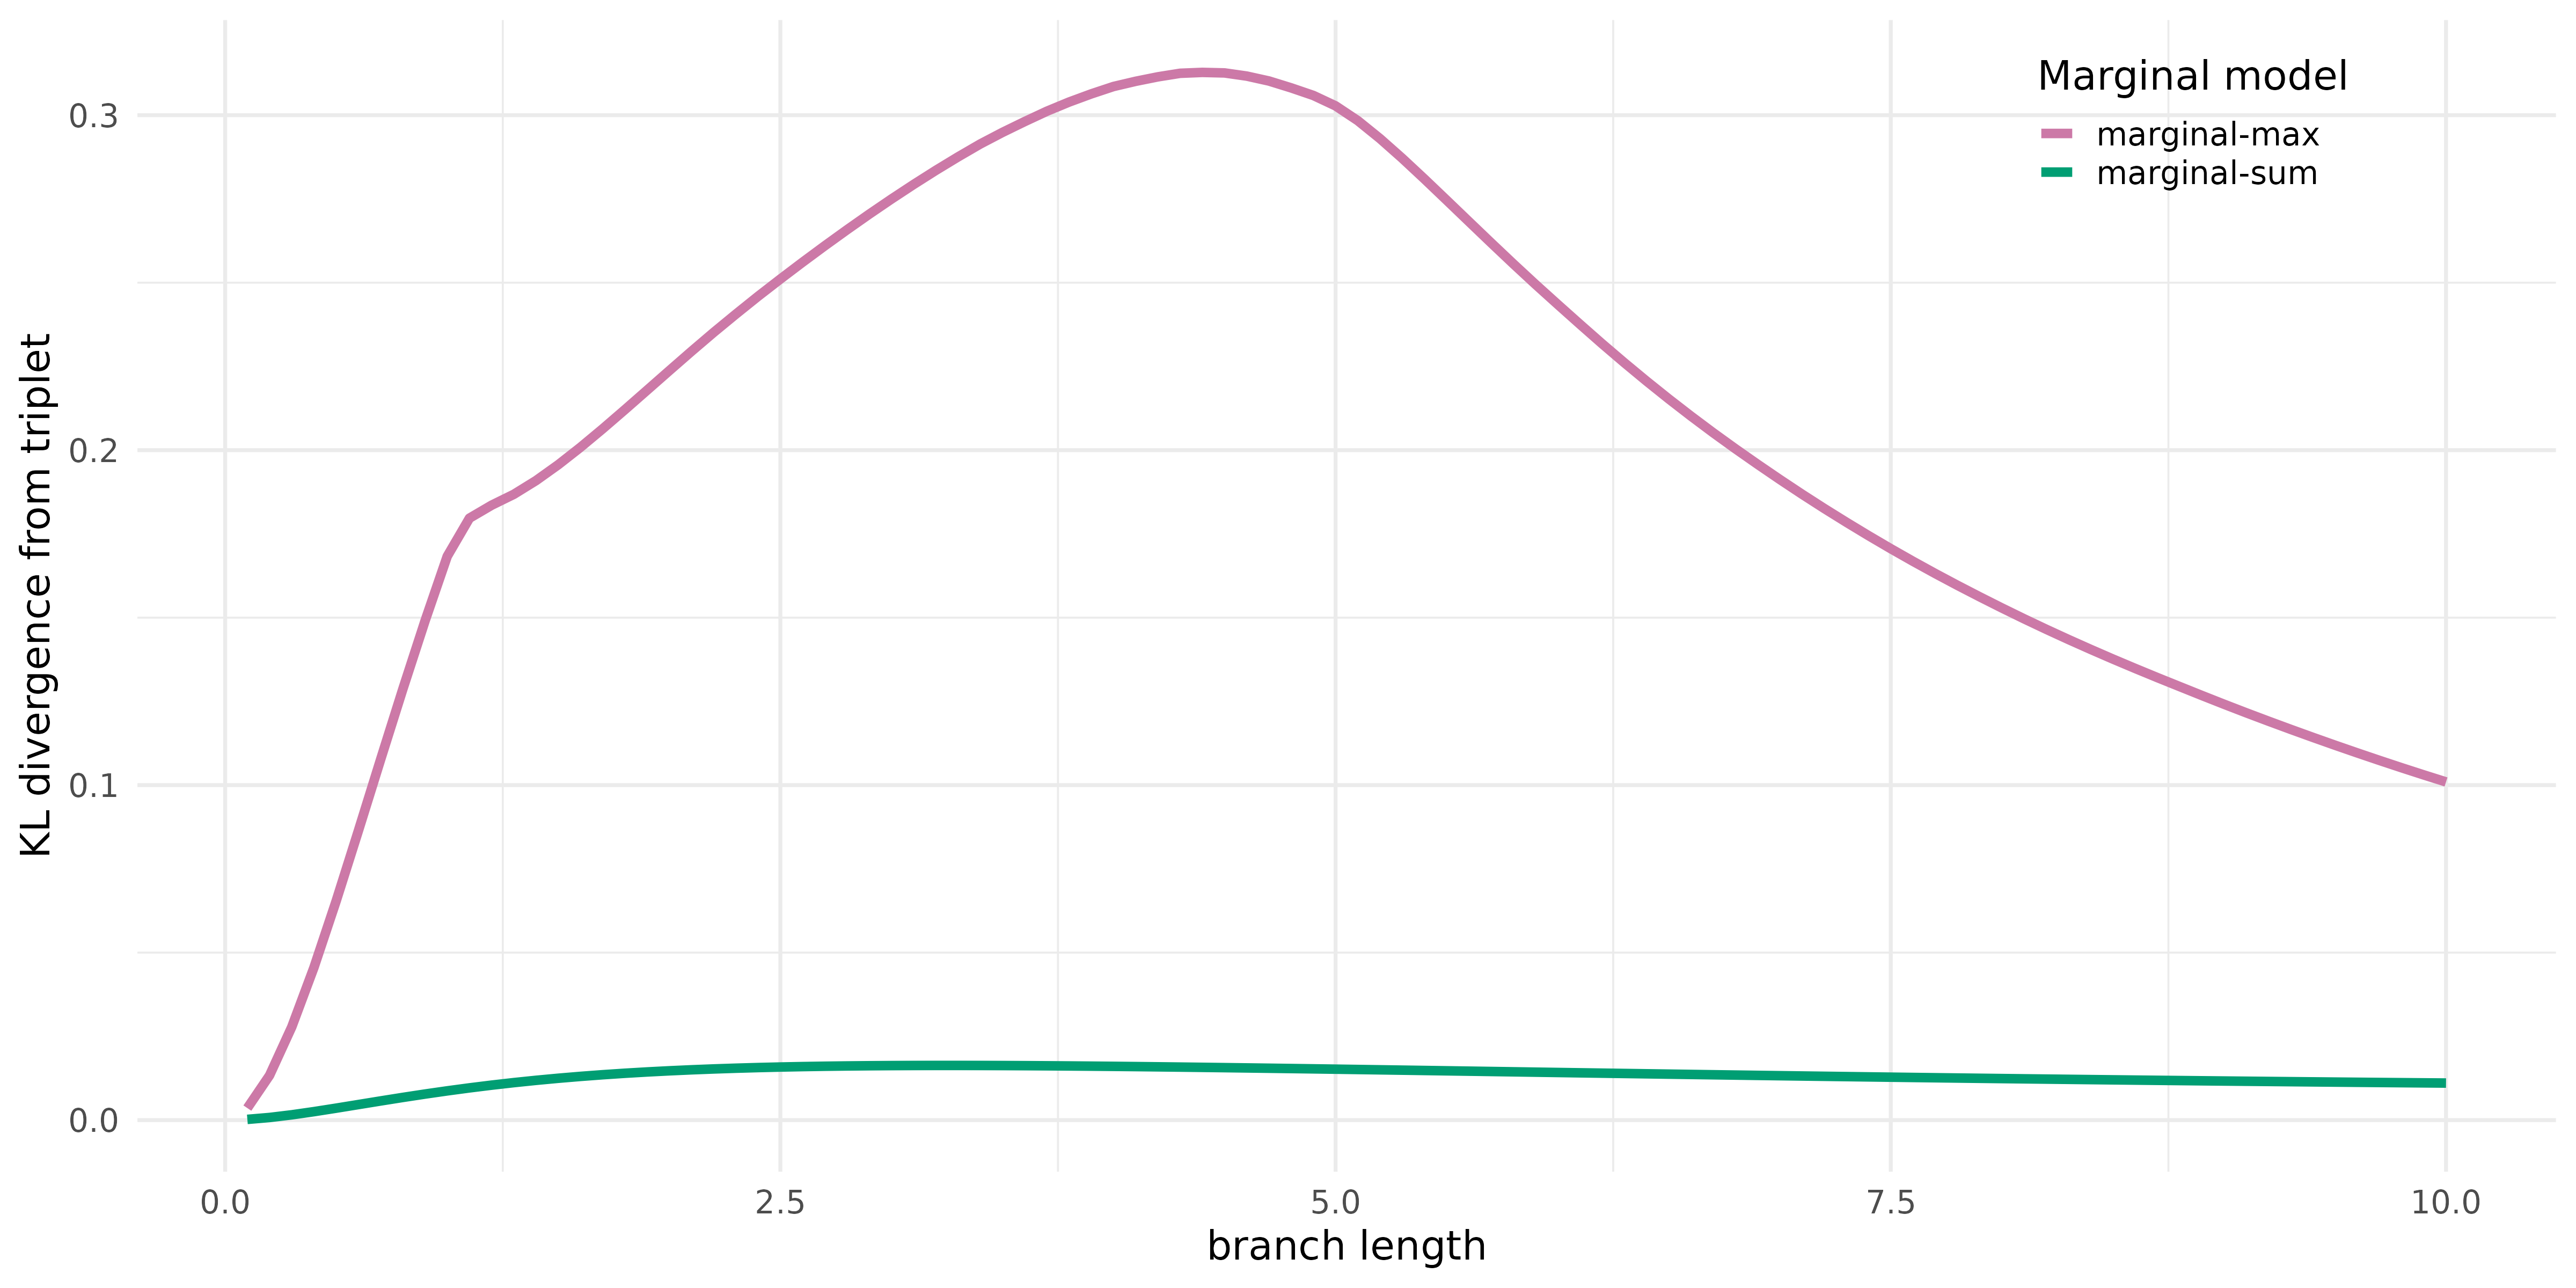
\includegraphics[height = 0.9\textheight]{defense/images/kld_mg.png}
\end{frame} %-------------------------------------------------------------------

\begin{frame}{Methods} %--------------------------------------------------------
    \begin{itemize}
        \item Compare how well the triplet, marginal-max, and marginal-max perform.
        \item Pipeline that simulates two descendants given a human CDS.
        \item Metrics: $d_{seq}$ and number of perfect and imperfect alignments.
    \end{itemize}
\centering
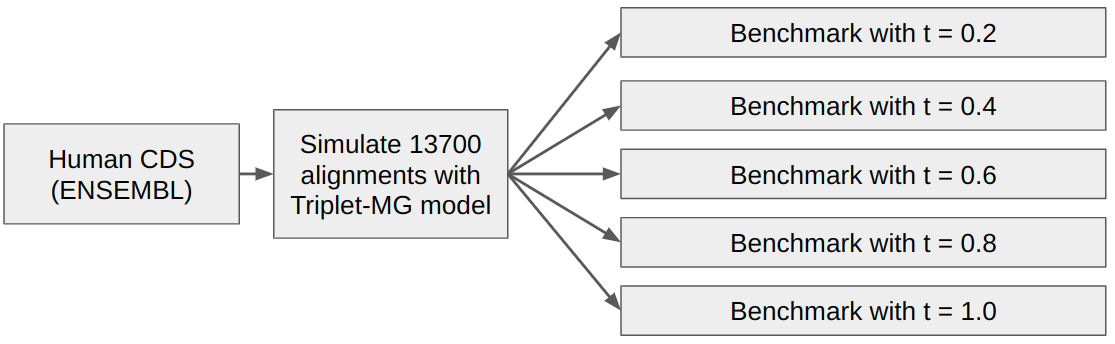
\includegraphics[width=0.8\textwidth]{/images/coati_evo_sim_chart.png}
\end{frame} %-------------------------------------------------------------------

\begin{frame}[c] %--------------------------------------------------------------
\centering
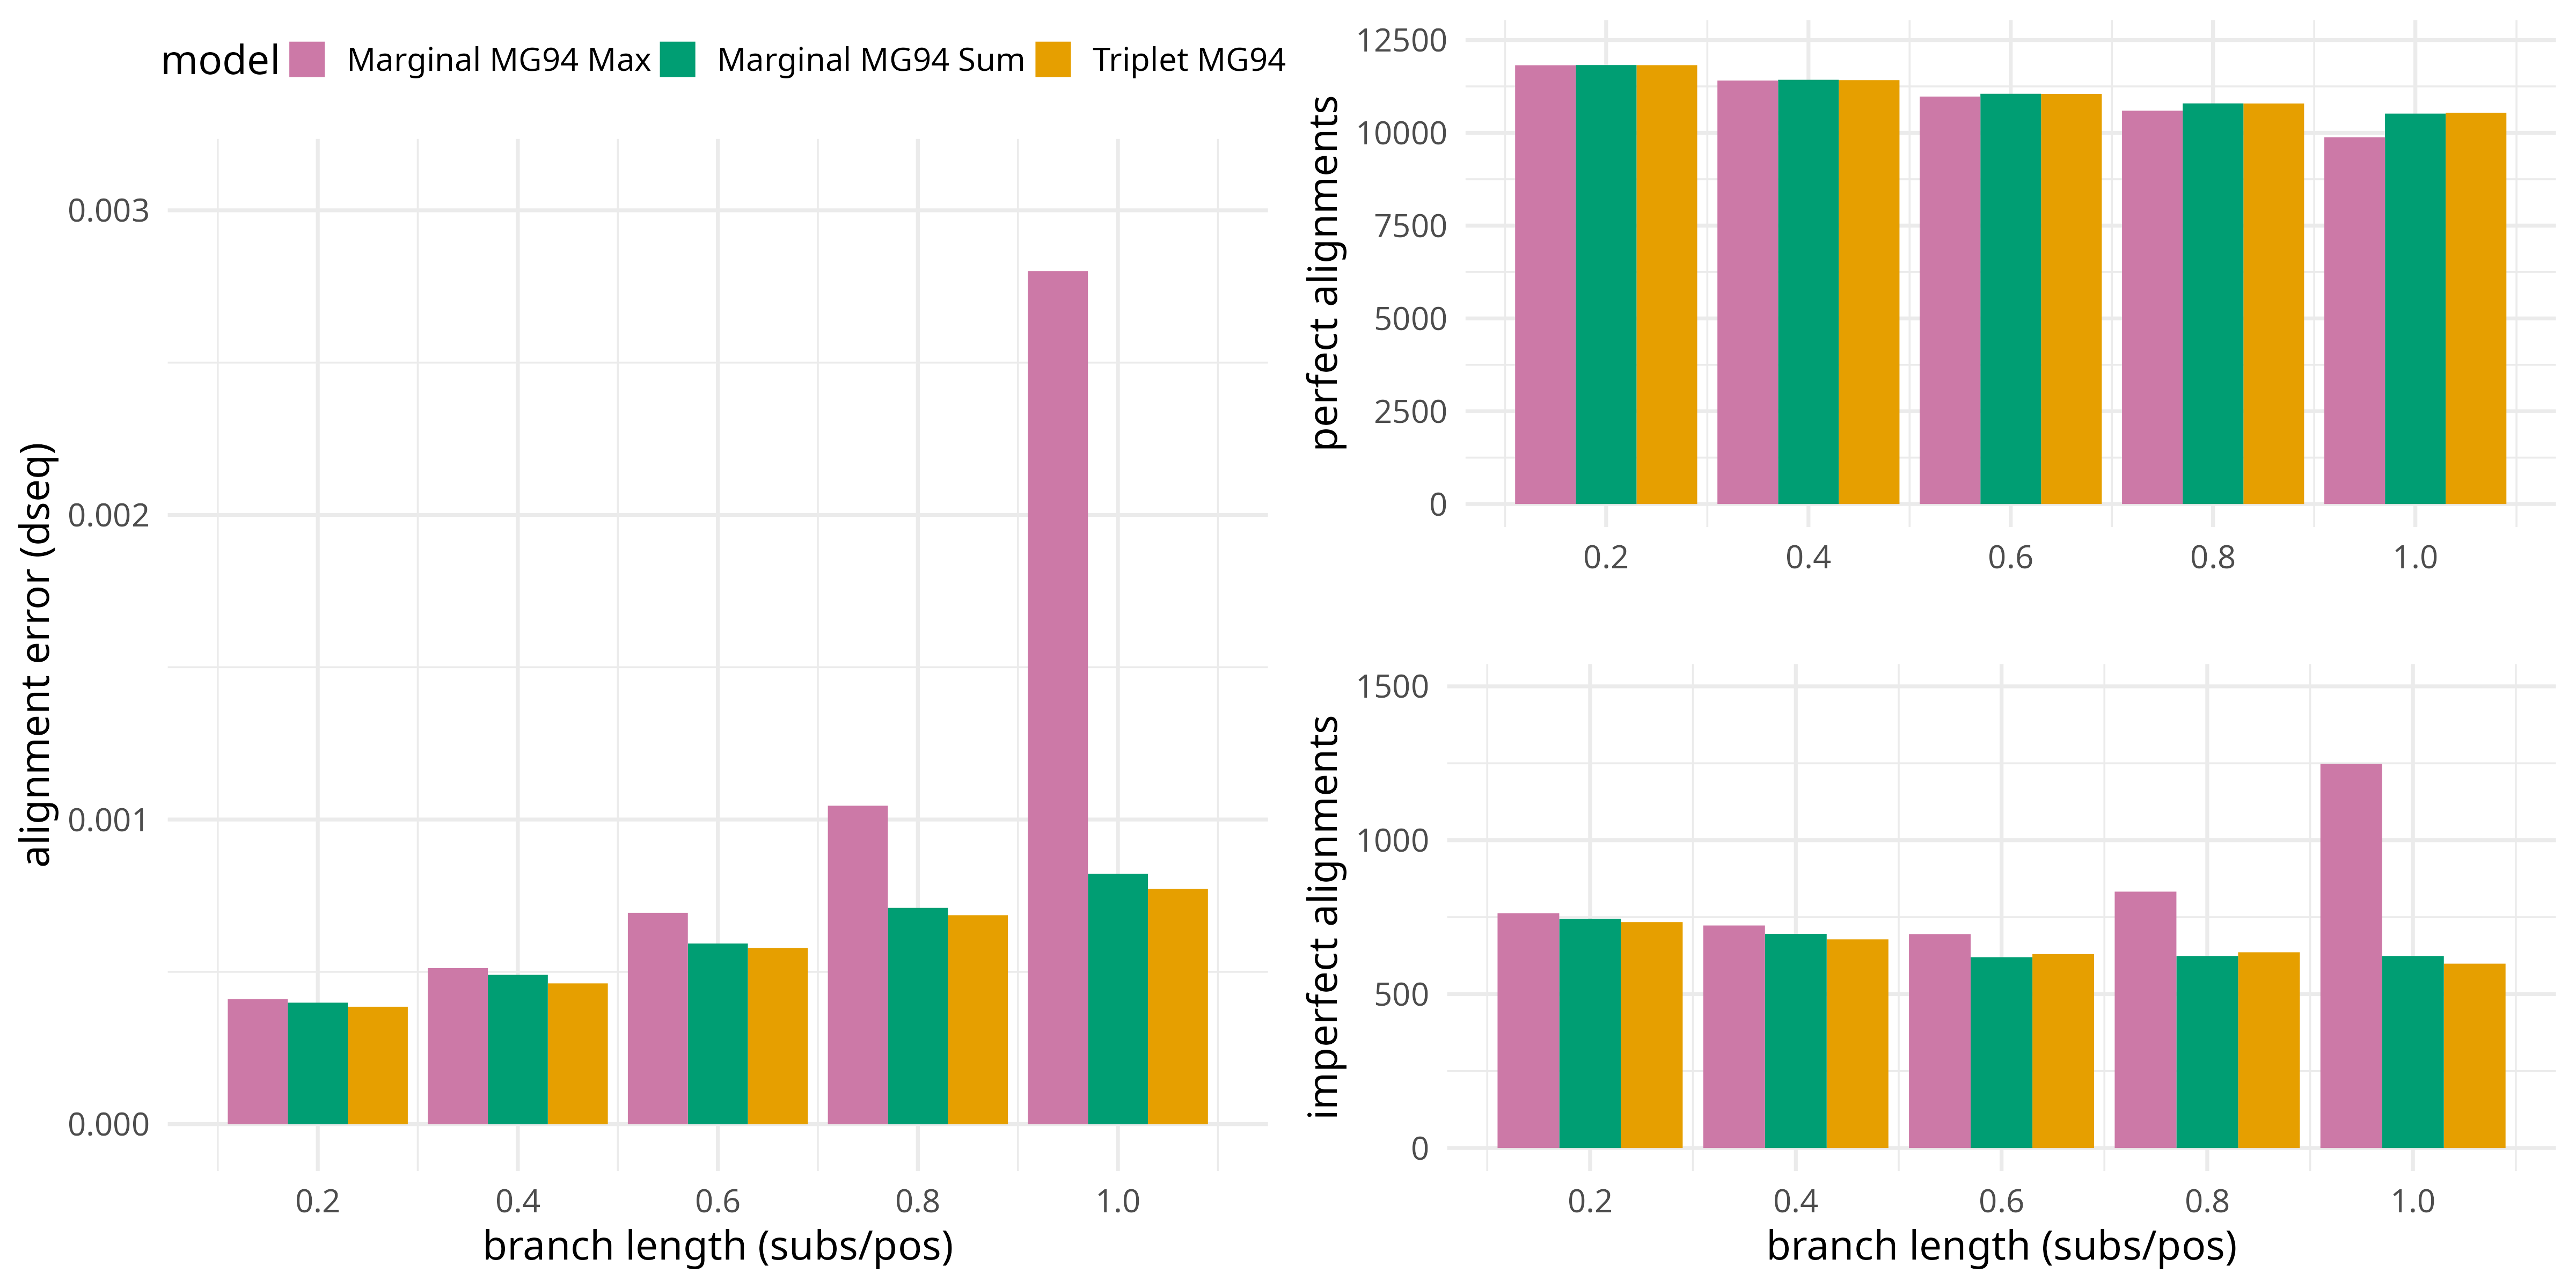
\includegraphics[height = 0.9\textheight]{defense/images/results_marginal_triplet_mg.png}
\note[item]{Transition: Marginal-sum is a good approximation, yet available metrics are not able to find where it differs from the triplet.}
\end{frame} %-------------------------------------------------------------------

\begin{frame}{AlnDotPlot} %-----------------------------------------------------
\begin{itemize}
    \item A tool to compare pairwise alignments inspired by traditional dot plots.
    \item Alignment event: matches, mismatches, and indels.
    \item Visualize sampling results.
    \item Identify and display subtle differences in long alignments.
    \item Examine codon similarity in alignment space.
\end{itemize}
\note[item]{I developed a tool to compare pairwise alignments inspired by traditional tod plots.}
\note[item]{AlnDotPlot can display single alignments, compare sampling results to analyze alignment space, find subtle differences in long alignments, and examine codon similarity.}
\end{frame} %-------------------------------------------------------------------

\begin{frame}[t]{Alignment to Dot Plot} %---------------------------------------
\begin{columns}
    \column{0.3\textwidth}
        \centering
        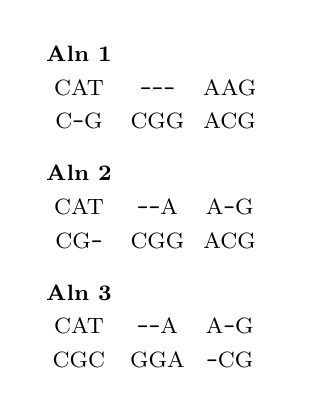
\begin{tikzpicture}[node distance=5mm,font=\footnotesize]
\tikzstyle{aln}=[matrix of nodes, nodes in empty cells]

\matrix (aln1)[aln] {
 \textbf{Aln 1} & & &\\
CAT & \verb|---| & AAG &\\
C\verb|-|G & CGG & ACG &\\
\\
 \textbf{Aln 2} & & &\\
CAT & \verb|--|A & A\verb|-|G &\\
CG\verb|-| & CGG & ACG &\\
\\
 \textbf{Aln 3} & & &\\
CAT & \verb|--|A & A\verb|-|G &\\
CGC & GGA & \verb|-|CG &\\
};
\end{tikzpicture}
    \column{0.7\textwidth}
        \only<1>{\resizebox{!}{0.8\textheight}{% Created by tikzDevice version 0.12.4 on 2023-10-07 18:20:52
% !TEX encoding = UTF-8 Unicode
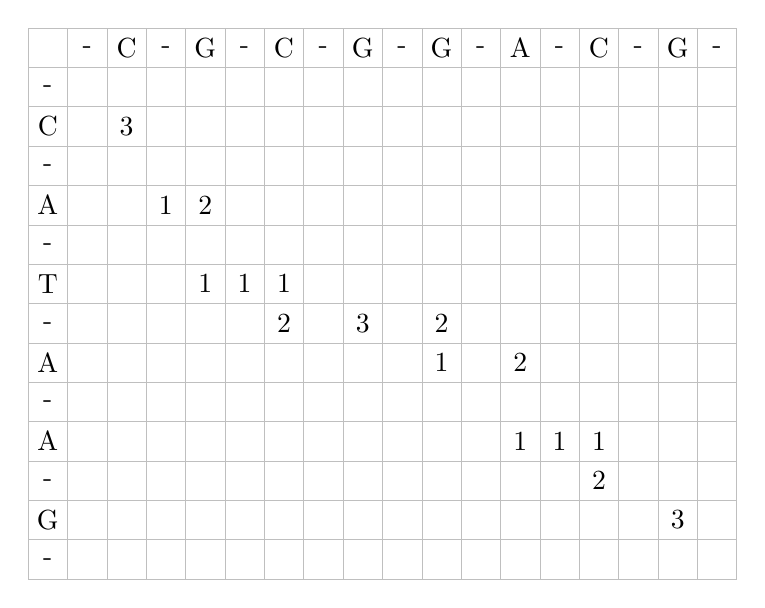
\begin{tikzpicture}[count/.style={color=black}]
\draw[very thin, color = gray!50, step = 0.5] (0,0) grid (9, 7);
\node at (0.25,6.25) {-};
\node at (0.25,5.75) {C};
\node at (0.25,5.25) {-};
\node at (0.25,4.75) {A};
\node at (0.25,4.25) {-};
\node at (0.25,3.75) {T};
\node at (0.25,3.25) {-};
\node at (0.25,2.75) {A};
\node at (0.25,2.25) {-};
\node at (0.25,1.75) {A};
\node at (0.25,1.25) {-};
\node at (0.25,0.75) {G};
\node at (0.25,0.25) {-};
\node at (0.75,6.75) {-};
\node at (1.25,6.75) {C};
\node at (1.75,6.75) {-};
\node at (2.25,6.75) {G};
\node at (2.75,6.75) {-};
\node at (3.25,6.75) {C};
\node at (3.75,6.75) {-};
\node at (4.25,6.75) {G};
\node at (4.75,6.75) {-};
\node at (5.25,6.75) {G};
\node at (5.75,6.75) {-};
\node at (6.25,6.75) {A};
\node at (6.75,6.75) {-};
\node at (7.25,6.75) {C};
\node at (7.75,6.75) {-};
\node at (8.25,6.75) {G};
\node at (8.75,6.75) {-};
% \node[count] at (0.75, 6.25){3};
\node[count] at (1.25, 5.75){3};
% \node[count] at (1.75, 5.25){3};
\node[count] at (1.75, 4.75){1};
\node[count] at (2.25, 4.75){2};
% \node[count] at (1.75, 4.25){1};
% \node[count] at (2.75, 4.25){2};
\node[count] at (2.25, 3.75){1};
\node[count] at (2.75, 3.75){1};
\node[count] at (3.25, 3.75){1};
% \node[count] at (2.75, 3.25){2};
\node[count] at (3.25, 3.25){2};
% \node[count] at (3.75, 3.25){3};
\node[count] at (4.25, 3.25){3};
% \node[count] at (4.75, 3.25){3};
\node[count] at (5.25, 3.25){2};
% \node[count] at (5.75, 3.25){2};
\node[count] at (5.25, 2.75){1};
\node[count] at (6.25, 2.75){2};
% \node[count] at (5.75, 2.25){1};
% \node[count] at (6.75, 2.25){2};
\node[count] at (6.25, 1.75){1};
\node[count] at (6.75, 1.75){1};
\node[count] at (7.25, 1.75){1};
% \node[count] at (6.75, 1.25){2};
\node[count] at (7.25, 1.25){2};
% \node[count] at (7.75, 1.25){3};
\node[count] at (8.25, 0.75){3};
% \node[count] at (8.75, 0.25){3};
\end{tikzpicture}
}}
        % \only<2>{\definecolor{color1}{HTML}{CC9966}
\definecolor{color2}{HTML}{99CCFF}
\definecolor{viridis0}{RGB}{255, 255, 255}
\definecolor{viridis1}{RGB}{253, 231, 37}
\definecolor{viridis2}{RGB}{181, 222, 43}
\definecolor{viridis3}{RGB}{110, 206, 88}
\definecolor{viridis4}{RGB}{53, 183, 121}
\definecolor{viridis5}{RGB}{31, 158, 137}
\definecolor{viridis6}{RGB}{38, 130, 142}
\definecolor{viridis7}{RGB}{49, 104, 142}
\definecolor{viridis8}{RGB}{62, 73, 137}
\definecolor{viridis9}{RGB}{72, 40, 120}
\definecolor{viridis10}{RGB}{68, 1, 84}
\begin{tikzpicture}[dot/.style={circle, minimum size=2.5mm}]
\draw[very thin, color = gray!50, step = 0.5] (0,0) grid (19, 16);
\node at (0.25,15.25) {-};
\node at (0.25,14.75) {C};
\node at (0.25,14.25) {-};
\node at (0.25,13.75) {A};
\node at (0.25,13.25) {-};
\node at (0.25,12.75) {T};
\node at (0.25,12.25) {-};
\node at (0.25,11.75) {A};
\node at (0.25,11.25) {-};
\node at (0.25,10.75) {A};
\node at (0.25,10.25) {-};
\node at (0.25,9.75) {G};
\node at (0.25,9.25) {-};
\node at (0.25,8.75) {C};
\node at (0.25,8.25) {-};
\node at (0.25,7.75) {G};
\node at (0.25,7.25) {-};
\node at (0.25,6.75) {G};
\node at (0.25,6.25) {-};
\node at (0.25,5.75) {T};
\node at (0.25,5.25) {-};
\node at (0.25,4.75) {C};
\node at (0.25,4.25) {-};
\node at (0.25,3.75) {G};
\node at (0.25,3.25) {-};
\node at (0.25,2.75) {G};
\node at (0.25,2.25) {-};
\node at (0.25,1.75) {A};
\node at (0.25,1.25) {-};
\node at (0.25,0.75) {C};
\node at (0.25,0.25) {-};
\node at (0.75,15.75) {-};
\node at (1.25,15.75) {C};
\node at (1.75,15.75) {-};
\node at (2.25,15.75) {A};
\node at (2.75,15.75) {-};
\node at (3.25,15.75) {G};
\node at (3.75,15.75) {-};
\node at (4.25,15.75) {C};
\node at (4.75,15.75) {-};
\node at (5.25,15.75) {G};
\node at (5.75,15.75) {-};
\node at (6.25,15.75) {G};
\node at (6.75,15.75) {-};
\node at (7.25,15.75) {T};
\node at (7.75,15.75) {-};
\node at (8.25,15.75) {C};
\node at (8.75,15.75) {-};
\node at (9.25,15.75) {C};
\node at (9.75,15.75) {-};
\node at (10.25,15.75) {C};
\node at (10.75,15.75) {-};
\node at (11.25,15.75) {C};
\node at (11.75,15.75) {-};
\node at (12.25,15.75) {G};
\node at (12.75,15.75) {-};
\node at (13.25,15.75) {G};
\node at (13.75,15.75) {-};
\node at (14.25,15.75) {A};
\node at (14.75,15.75) {-};
\node at (15.25,15.75) {C};
\node at (15.75,15.75) {-};
\node at (16.25,15.75) {A};
\node at (16.75,15.75) {-};
\node at (17.25,15.75) {C};
\node at (17.75,15.75) {-};
\node at (18.25,15.75) {G};
\node at (18.75,15.75) {-};
\draw[line width=1.25mm,viridis10](0.75,15.25)--(1.25,14.75);
\draw[line width=1.25mm,viridis10](1.25,14.75)--(1.75,14.25);
\node[circle, fill=viridis10] at (1.25, 14.75){};
\draw[line width=1.25mm,viridis10](1.75,14.25)--(2.25,13.75);
\draw[line width=1.25mm,viridis10](2.25,13.75)--(2.75,13.25);
\node[circle, fill=viridis10] at (2.25, 13.75){};
\draw[line width=1.25mm,viridis4](2.75,13.25)--(2.75,12.75);
\draw[line width=1.25mm,viridis7](2.75,13.25)--(3.25,12.75);
\draw[line width=1.25mm,viridis4](2.75,12.75)--(2.75,12.25);
\node[circle, fill=viridis4] at (2.75, 12.75){};
\draw[line width=1.25mm,viridis7](3.25,12.75)--(3.75,12.25);
\node[circle, fill=viridis7] at (3.25, 12.75){};
\draw[line width=1.25mm,viridis4](2.75,12.25)--(2.75,11.75);
\draw[line width=1.25mm,viridis7](3.75,12.25)--(4.25,11.75);
\draw[line width=1.25mm,viridis4](2.75,11.75)--(2.75,11.25);
\node[circle, fill=viridis4] at (2.75, 11.75){};
\draw[line width=1.25mm,viridis7](4.25,11.75)--(4.75,11.25);
\node[circle, fill=viridis7] at (4.25, 11.75){};
\draw[line width=1.25mm,viridis4](2.75,11.25)--(2.75,10.75);
\draw[line width=1.25mm,viridis7](4.75,11.25)--(5.25,10.75);
\draw[line width=1.25mm,viridis4](2.75,10.75)--(2.75,10.25);
\node[circle, fill=viridis4] at (2.75, 10.75){};
\draw[line width=1.25mm,viridis7](5.25,10.75)--(5.75,10.25);
\node[circle, fill=viridis7] at (5.25, 10.75){};
\draw[line width=1.25mm,viridis4](2.75,10.25)--(3.25,9.75);
\draw[line width=1.25mm,viridis7](5.75,10.25)--(6.25,9.75);
\draw[line width=1.25mm,viridis4](3.25,9.75)--(3.75,9.25);
\node[circle, fill=viridis4] at (3.25, 9.75){};
\draw[line width=1.25mm,viridis7](6.25,9.75)--(6.75,9.25);
\node[circle, fill=viridis7] at (6.25, 9.75){};
\draw[line width=1.25mm,viridis4](3.75,9.25)--(4.25,8.75);
\draw[line width=1.25mm,viridis7](6.75,9.25)--(7.25,8.75);
\draw[line width=1.25mm,viridis4](4.25,8.75)--(4.75,8.25);
\node[circle, fill=viridis4] at (4.25, 8.75){};
\draw[line width=1.25mm,viridis7](7.25,8.75)--(7.75,8.25);
\node[circle, fill=viridis7] at (7.25, 8.75){};
\draw[line width=1.25mm,viridis4](4.75,8.25)--(5.25,7.75);
\draw[line width=1.25mm,viridis7](7.75,8.25)--(8.25,7.75);
\draw[line width=1.25mm,viridis4](5.25,7.75)--(5.75,7.25);
\node[circle, fill=viridis4] at (5.25, 7.75){};
\draw[line width=1.25mm,viridis7](8.25,7.75)--(8.75,7.25);
\node[circle, fill=viridis7] at (8.25, 7.75){};
\draw[line width=1.25mm,viridis4](5.75,7.25)--(6.25,6.75);
\draw[line width=1.25mm,viridis7](8.75,7.25)--(9.25,6.75);
\draw[line width=1.25mm,viridis4](6.25,6.75)--(6.75,6.25);
\node[circle, fill=viridis4] at (6.25, 6.75){};
\draw[line width=1.25mm,viridis7](9.25,6.75)--(9.75,6.25);
\node[circle, fill=viridis7] at (9.25, 6.75){};
\draw[line width=1.25mm,viridis4](6.75,6.25)--(7.25,5.75);
\draw[line width=1.25mm,viridis7](9.75,6.25)--(10.25,5.75);
\draw[line width=1.25mm,viridis4](7.25,5.75)--(7.75,5.25);
\node[circle, fill=viridis4] at (7.25, 5.75){};
\draw[line width=1.25mm,viridis7](10.25,5.75)--(10.75,5.25);
\node[circle, fill=viridis7] at (10.25, 5.75){};
\draw[line width=1.25mm,viridis4](7.75,5.25)--(8.25,4.75);
\draw[line width=1.25mm,viridis7](10.75,5.25)--(11.25,4.75);
\draw[line width=1.25mm,viridis4](8.25,4.75)--(8.75,4.25);
\node[circle, fill=viridis4] at (8.25, 4.75){};
\draw[line width=1.25mm,viridis7](11.25,4.75)--(11.75,4.25);
\node[circle, fill=viridis7] at (11.25, 4.75){};
\draw[line width=1.25mm,viridis4](8.75,4.25)--(9.25,4.25);
\draw[line width=1.25mm,viridis4](9.25,4.25)--(9.75,4.25);
\node[circle, fill=viridis4] at (9.25, 4.25){};
\draw[line width=1.25mm,viridis4](9.75,4.25)--(10.25,4.25);
\draw[line width=1.25mm,viridis4](10.25,4.25)--(10.75,4.25);
\node[circle, fill=viridis4] at (10.25, 4.25){};
\draw[line width=1.25mm,viridis4](10.75,4.25)--(11.25,4.25);
\draw[line width=1.25mm,viridis4](11.25,4.25)--(11.75,4.25);
\node[circle, fill=viridis4] at (11.25, 4.25){};
\draw[line width=1.25mm,viridis4](11.75,4.25)--(12.25,4.25);
\draw[line width=1.25mm,viridis7](11.75,4.25)--(12.25,3.75);
\draw[line width=1.25mm,viridis4](12.25,4.25)--(12.75,4.25);
\node[circle, fill=viridis4] at (12.25, 4.25){};
\draw[line width=1.25mm,viridis4](12.75,4.25)--(13.25,4.25);
\draw[line width=1.25mm,viridis4](13.25,4.25)--(13.75,4.25);
\node[circle, fill=viridis4] at (13.25, 4.25){};
\draw[line width=1.25mm,viridis4](13.75,4.25)--(14.25,4.25);
\draw[line width=1.25mm,viridis4](14.25,4.25)--(14.75,4.25);
\node[circle, fill=viridis4] at (14.25, 4.25){};
\draw[line width=1.25mm,viridis4](14.75,4.25)--(15.25,3.75);
\draw[line width=1.25mm,viridis7](12.25,3.75)--(12.75,3.25);
\node[circle, fill=viridis7] at (12.25, 3.75){};
\draw[line width=1.25mm,viridis4](15.25,3.75)--(15.75,3.25);
\node[circle, fill=viridis4] at (15.25, 3.75){};
\draw[line width=1.25mm,viridis7](12.75,3.25)--(13.25,2.75);
\draw[line width=1.25mm,viridis4](15.75,3.25)--(16.25,2.75);
\draw[line width=1.25mm,viridis7](13.25,2.75)--(13.75,2.25);
\node[circle, fill=viridis7] at (13.25, 2.75){};
\draw[line width=1.25mm,viridis4](16.25,2.75)--(16.75,2.25);
\node[circle, fill=viridis4] at (16.25, 2.75){};
\draw[line width=1.25mm,viridis7](13.75,2.25)--(14.25,1.75);
\draw[line width=1.25mm,viridis4](16.75,2.25)--(17.25,1.75);
\draw[line width=1.25mm,viridis7](14.25,1.75)--(14.75,1.25);
\node[circle, fill=viridis7] at (14.25, 1.75){};
\draw[line width=1.25mm,viridis4](17.25,1.75)--(17.75,1.25);
\node[circle, fill=viridis4] at (17.25, 1.75){};
\draw[line width=1.25mm,viridis7](14.75,1.25)--(15.25,0.75);
\draw[line width=1.25mm,viridis4](17.75,1.25)--(18.25,0.75);
\draw[line width=1.25mm,viridis7](15.25,0.75)--(15.75,0.25);
\node[circle, fill=viridis7] at (15.25, 0.75){};
\draw[line width=1.25mm,viridis4](18.25,0.75)--(18.75,0.25);
\node[circle, fill=viridis4] at (18.25, 0.75){};
\draw[line width=1.25mm,viridis7](15.75,0.25)--(16.25,0.25);
\draw[line width=1.25mm,viridis7](16.25,0.25)--(16.75,0.25);
\node[circle, fill=viridis7] at (16.25, 0.25){};
\draw[line width=1.25mm,viridis7](16.75,0.25)--(17.25,0.25);
\draw[line width=1.25mm,viridis7](17.25,0.25)--(17.75,0.25);
\node[circle, fill=viridis7] at (17.25, 0.25){};
\draw[line width=1.25mm,viridis7](17.75,0.25)--(18.25,0.25);
\draw[line width=1.25mm,viridis7](18.25,0.25)--(18.75,0.25);
\node[circle, fill=viridis7] at (18.25, 0.25){};
\matrix [draw, below right, draw=none] at (current bounding box.north east) {
        % \node[circle, fill=viridis0, scale=0.75] {0\%}; \\
        \node[circle, fill=viridis1, scale=0.75] {00-09\%}; \\
        \node[circle, fill=viridis2, scale=0.75] {10-19\%}; \\
        \node[circle, fill=viridis3, scale=0.75] {20-29\%}; \\
        \node[circle, fill=viridis4, scale=0.75] {30-29\%}; \\
        \node[circle, fill=viridis5, scale=0.75] {\textcolor{white}{40-49\%}}; \\
        \node[circle, fill=viridis6, scale=0.75] {\textcolor{white}{50-59\%}}; \\
        \node[circle, fill=viridis7, scale=0.75] {\textcolor{white}{60-69\%}}; \\
        \node[circle, fill=viridis8, scale=0.75] {\textcolor{white}{70-79\%}}; \\
        \node[circle, fill=viridis9, scale=0.75] {\textcolor{white}{80-89\%}}; \\
        \node[circle, fill=viridis10, scale=0.75] {\textcolor{white}{90-100\%}}; \\
    };
\end{tikzpicture}
}
        \only<2>{\resizebox{\textwidth}{!}{% Created by tikzDevice version 0.12.5 on 2023-10-23 22:31:07
% !TEX encoding = UTF-8 Unicode
\definecolor{color1}{HTML}{CC9966}
\definecolor{color2}{HTML}{99CCFF}
\definecolor{viridis0}{RGB}{255, 255, 255}
\definecolor{viridis1}{RGB}{253, 231, 37}
\definecolor{viridis2}{RGB}{181, 222, 43}
\definecolor{viridis3}{RGB}{110, 206, 88}
\definecolor{viridis4}{RGB}{53, 183, 121}
\definecolor{viridis5}{RGB}{31, 158, 137}
\definecolor{viridis6}{RGB}{38, 130, 142}
\definecolor{viridis7}{RGB}{49, 104, 142}
\definecolor{viridis8}{RGB}{62, 73, 137}
\definecolor{viridis9}{RGB}{72, 40, 120}
\definecolor{viridis10}{RGB}{68, 1, 84}
\begin{tikzpicture}[dot/.style={circle, minimum size=2.5mm}]
\draw[very thin, color = gray!50, step = 0.5] (0,0) grid (9, 7);
\node at (0.25,6.25) {-};
\node at (0.25,5.75) {C};
\node at (0.25,5.25) {-};
\node at (0.25,4.75) {A};
\node at (0.25,4.25) {-};
\node at (0.25,3.75) {T};
\node at (0.25,3.25) {-};
\node at (0.25,2.75) {A};
\node at (0.25,2.25) {-};
\node at (0.25,1.75) {A};
\node at (0.25,1.25) {-};
\node at (0.25,0.75) {G};
\node at (0.25,0.25) {-};
\node at (0.75,6.75) {-};
\node at (1.25,6.75) {C};
\node at (1.75,6.75) {-};
\node at (2.25,6.75) {G};
\node at (2.75,6.75) {-};
\node at (3.25,6.75) {C};
\node at (3.75,6.75) {-};
\node at (4.25,6.75) {G};
\node at (4.75,6.75) {-};
\node at (5.25,6.75) {G};
\node at (5.75,6.75) {-};
\node at (6.25,6.75) {A};
\node at (6.75,6.75) {-};
\node at (7.25,6.75) {C};
\node at (7.75,6.75) {-};
\node at (8.25,6.75) {G};
\node at (8.75,6.75) {-};
\draw[line width=1.25mm,viridis10](0.75,6.25)--(1.25,5.75);
\draw[line width=1.25mm,viridis10](1.25,5.75)--(1.75,5.25);
\node[circle, fill=viridis10] at (1.25, 5.75){};
\node[white] at (1.25, 5.75) {$\mathlarger{\mathlarger{\bm{\times}}}$};
\draw[line width=1.25mm,viridis4](1.75,5.25)--(1.75,4.75);
\draw[line width=1.25mm,viridis7](1.75,5.25)--(2.25,4.75);
\draw[line width=1.25mm,viridis4](1.75,4.75)--(1.75,4.25);
\node[circle, fill=viridis4] at (1.75, 4.75){};
\draw[line width=1.25mm,viridis7](2.25,4.75)--(2.75,4.25);
\node[circle, fill=viridis7] at (2.25, 4.75){};
\draw[line width=1.25mm,viridis4](1.75,4.25)--(2.25,3.75);
\draw[line width=1.25mm,viridis4](2.75,4.25)--(2.75,3.75);
\draw[line width=1.25mm,viridis4](2.75,4.25)--(3.25,3.75);
\draw[line width=1.25mm,viridis4](2.25,3.75)--(2.75,3.25);
\node[circle, fill=viridis4] at (2.25, 3.75){};
\draw[line width=1.25mm,viridis4](2.75,3.75)--(2.75,3.25);
\node[circle, fill=viridis4] at (2.75, 3.75){};
\draw[line width=1.25mm,viridis4](3.25,3.75)--(3.75,3.25);
\node[circle, fill=viridis4] at (3.25, 3.75){};
\draw[line width=1.25mm,viridis7](2.75,3.25)--(3.25,3.25);
\draw[line width=1.25mm,viridis7](3.25,3.25)--(3.75,3.25);
\node[circle, fill=viridis7] at (3.25, 3.25){};
\draw[line width=1.25mm,viridis10](3.75,3.25)--(4.25,3.25);
\draw[line width=1.25mm,viridis10](4.25,3.25)--(4.75,3.25);
\node[circle, fill=viridis10] at (4.25, 3.25){};
\draw[line width=1.25mm,viridis7](4.75,3.25)--(5.25,3.25);
\draw[line width=1.25mm,viridis4](4.75,3.25)--(5.25,2.75);
\draw[line width=1.25mm,viridis7](5.25,3.25)--(5.75,3.25);
\node[circle, fill=viridis7] at (5.25, 3.25){};
\draw[line width=1.25mm,viridis7](5.75,3.25)--(6.25,2.75);
\draw[line width=1.25mm,viridis4](5.25,2.75)--(5.75,2.25);
\node[circle, fill=viridis4] at (5.25, 2.75){};
\draw[line width=1.25mm,viridis7](6.25,2.75)--(6.75,2.25);
\node[circle, fill=viridis7] at (6.25, 2.75){};
\node[white] at (6.25, 2.75) {$\mathlarger{\mathlarger{\bm{\times}}}$};
\draw[line width=1.25mm,viridis4](5.75,2.25)--(6.25,1.75);
\draw[line width=1.25mm,viridis4](6.75,2.25)--(6.75,1.75);
\draw[line width=1.25mm,viridis4](6.75,2.25)--(7.25,1.75);
\draw[line width=1.25mm,viridis4](6.25,1.75)--(6.75,1.25);
\node[circle, fill=viridis4] at (6.25, 1.75){};
\node[white] at (6.25, 1.75) {$\mathlarger{\mathlarger{\bm{\times}}}$};
\draw[line width=1.25mm,viridis4](6.75,1.75)--(6.75,1.25);
\node[circle, fill=viridis4] at (6.75, 1.75){};
\draw[line width=1.25mm,viridis4](7.25,1.75)--(7.75,1.25);
\node[circle, fill=viridis4] at (7.25, 1.75){};
\draw[line width=1.25mm,viridis7](6.75,1.25)--(7.25,1.25);
\draw[line width=1.25mm,viridis7](7.25,1.25)--(7.75,1.25);
\node[circle, fill=viridis7] at (7.25, 1.25){};
\draw[line width=1.25mm,viridis10](7.75,1.25)--(8.25,0.75);
\draw[line width=1.25mm,viridis10](8.25,0.75)--(8.75,0.25);
\node[circle, fill=viridis10] at (8.25, 0.75){};
\node[white] at (8.25, 0.75) {$\mathlarger{\mathlarger{\bm{\times}}}$};
\matrix [draw, below right, draw=none] at (current bounding box.north east) {
        % \node[circle, fill=viridis0, scale=0.75] {0\%}; \\
        \node[circle, fill=viridis1, scale=0.42] {00-09\%}; \\
        \node[circle, fill=viridis2, scale=0.42] {10-19\%}; \\
        \node[circle, fill=viridis3, scale=0.42] {20-29\%}; \\
        \node[circle, fill=viridis4, scale=0.42] {30-29\%}; \\
        \node[circle, fill=viridis5, scale=0.42] {\textcolor{white}{40-49\%}}; \\
        \node[circle, fill=viridis6, scale=0.42] {\textcolor{white}{50-59\%}}; \\
        \node[circle, fill=viridis7, scale=0.42] {\textcolor{white}{60-69\%}}; \\
        \node[circle, fill=viridis8, scale=0.42] {\textcolor{white}{70-79\%}}; \\
        \node[circle, fill=viridis9, scale=0.42] {\textcolor{white}{80-89\%}}; \\
        \node[circle, fill=viridis10, scale=0.42] {\textcolor{white}{90-100\%}}; \\
    };
\end{tikzpicture}
}}
\end{columns}
\note[item]{Rows and columns correspond to symbols in the sequences with empty spaces between them to mark insertions and deletions in the matrix (when appropriate).}
\note[item]{In this case, where we have 3 possible alignments of the same pair of sequences, we can count the number of each event <explain figure>.}
\note[item]{If we now represent those counts as frequency and color them, we obtain a graphical representation of the 3 alignments.}
\note[item]{Dots correspond to events in the alignments, edges join them to make a path. Xs mark matches and color represent their frequency.}
\note[item]{Explain figure.}
\end{frame} %-------------------------------------------------------------------

\begin{frame}[c]{Sampling} %----------------------------------------------------
\centering
\resizebox{!}{0.9\textheight}{% Created by tikzDevice version 0.12.5 on 2023-10-23 22:50:51
% !TEX encoding = UTF-8 Unicode
\definecolor{color1}{HTML}{CC9966}
\definecolor{color2}{HTML}{99CCFF}
\definecolor{viridis0}{RGB}{255, 255, 255}
\definecolor{viridis1}{RGB}{253, 231, 37}
\definecolor{viridis2}{RGB}{181, 222, 43}
\definecolor{viridis3}{RGB}{110, 206, 88}
\definecolor{viridis4}{RGB}{53, 183, 121}
\definecolor{viridis5}{RGB}{31, 158, 137}
\definecolor{viridis6}{RGB}{38, 130, 142}
\definecolor{viridis7}{RGB}{49, 104, 142}
\definecolor{viridis8}{RGB}{62, 73, 137}
\definecolor{viridis9}{RGB}{72, 40, 120}
\definecolor{viridis10}{RGB}{68, 1, 84}
\begin{tikzpicture}[dot/.style={circle, minimum size=2.5mm}]
\draw[very thin, color = gray!50, step = 0.5] (0,0) grid (9, 7);
\node at (0.25,6.25) {-};
\node at (0.25,5.75) {C};
\node at (0.25,5.25) {-};
\node at (0.25,4.75) {A};
\node at (0.25,4.25) {-};
\node at (0.25,3.75) {T};
\node at (0.25,3.25) {-};
\node at (0.25,2.75) {A};
\node at (0.25,2.25) {-};
\node at (0.25,1.75) {A};
\node at (0.25,1.25) {-};
\node at (0.25,0.75) {G};
\node at (0.25,0.25) {-};
\node at (0.75,6.75) {-};
\node at (1.25,6.75) {C};
\node at (1.75,6.75) {-};
\node at (2.25,6.75) {G};
\node at (2.75,6.75) {-};
\node at (3.25,6.75) {C};
\node at (3.75,6.75) {-};
\node at (4.25,6.75) {G};
\node at (4.75,6.75) {-};
\node at (5.25,6.75) {G};
\node at (5.75,6.75) {-};
\node at (6.25,6.75) {A};
\node at (6.75,6.75) {-};
\node at (7.25,6.75) {C};
\node at (7.75,6.75) {-};
\node at (8.25,6.75) {G};
\node at (8.75,6.75) {-};
\draw[line width=1.25mm,viridis1](0.75,6.25)--(1.25,6.25);
\draw[line width=1.25mm,viridis10](0.75,6.25)--(1.25,5.75);
\draw[line width=1.25mm,viridis1](1.25,6.25)--(1.75,6.25);
\node[circle, fill=viridis1] at (1.25, 6.25){};
\draw[line width=1.25mm,viridis1](1.75,6.25)--(2.25,6.25);
\draw[line width=1.25mm,viridis1](2.25,6.25)--(2.75,6.25);
\node[circle, fill=viridis1] at (2.25, 6.25){};
\draw[line width=1.25mm,viridis1](2.75,6.25)--(3.25,6.25);
\draw[line width=1.25mm,viridis1](2.75,6.25)--(3.25,5.75);
\draw[line width=1.25mm,viridis1](3.25,6.25)--(3.75,6.25);
\node[circle, fill=viridis1] at (3.25, 6.25){};
\draw[line width=1.25mm,viridis1](3.75,6.25)--(4.25,6.25);
\draw[line width=1.25mm,viridis1](4.25,6.25)--(4.75,6.25);
\node[circle, fill=viridis1] at (4.25, 6.25){};
\draw[line width=1.25mm,viridis1](4.75,6.25)--(5.25,6.25);
\draw[line width=1.25mm,viridis1](4.75,6.25)--(5.25,5.75);
\draw[line width=1.25mm,viridis1](5.25,6.25)--(5.75,6.25);
\node[circle, fill=viridis1] at (5.25, 6.25){};
\draw[line width=1.25mm,viridis1](5.75,6.25)--(6.25,6.25);
\draw[line width=1.25mm,viridis1](6.25,6.25)--(6.75,6.25);
\node[circle, fill=viridis1] at (6.25, 6.25){};
\draw[line width=1.25mm,viridis1](6.75,6.25)--(7.25,6.25);
\draw[line width=1.25mm,viridis1](6.75,6.25)--(7.25,5.75);
\draw[line width=1.25mm,viridis1](7.25,6.25)--(7.75,6.25);
\node[circle, fill=viridis1] at (7.25, 6.25){};
\draw[line width=1.25mm,viridis1](7.75,6.25)--(7.75,5.75);
\draw[line width=1.25mm,viridis10](1.25,5.75)--(1.75,5.25);
\node[circle, fill=viridis10] at (1.25, 5.75){};
\node[white] at (1.25, 5.75){$\mathlarger{\mathlarger{\bm{\times}}}$};
\draw[line width=1.25mm,viridis1](3.25,5.75)--(3.75,5.25);
\node[circle, fill=viridis1] at (3.25, 5.75){};
\node[black] at (3.25, 5.75){$\mathlarger{\mathlarger{\bm{\times}}}$};
\draw[line width=1.25mm,viridis1](5.25,5.75)--(5.75,5.25);
\node[circle, fill=viridis1] at (5.25, 5.75){};
\draw[line width=1.25mm,viridis1](7.25,5.75)--(7.75,5.25);
\node[circle, fill=viridis1] at (7.25, 5.75){};
\node[black] at (7.25, 5.75){$\mathlarger{\mathlarger{\bm{\times}}}$};
\draw[line width=1.25mm,viridis1](7.75,5.75)--(7.75,5.25);
\node[circle, fill=viridis1] at (7.75, 5.75){};
\draw[line width=1.25mm,viridis2](1.75,5.25)--(2.25,5.25);
\draw[line width=1.25mm,viridis1](1.75,5.25)--(1.75,4.75);
\draw[line width=1.25mm,viridis7](1.75,5.25)--(2.25,4.75);
\draw[line width=1.25mm,viridis2](2.25,5.25)--(2.75,5.25);
\node[circle, fill=viridis2] at (2.25, 5.25){};
\draw[line width=1.25mm,viridis2](2.75,5.25)--(3.25,5.25);
\draw[line width=1.25mm,viridis2](3.25,5.25)--(3.75,5.25);
\node[circle, fill=viridis2] at (3.25, 5.25){};
\draw[line width=1.25mm,viridis2](3.75,5.25)--(4.25,5.25);
\draw[line width=1.25mm,viridis1](3.75,5.25)--(4.25,4.75);
\draw[line width=1.25mm,viridis2](4.25,5.25)--(4.75,5.25);
\node[circle, fill=viridis2] at (4.25, 5.25){};
\draw[line width=1.25mm,viridis2](4.75,5.25)--(5.25,5.25);
\draw[line width=1.25mm,viridis2](5.25,5.25)--(5.75,5.25);
\node[circle, fill=viridis2] at (5.25, 5.25){};
\draw[line width=1.25mm,viridis1](5.75,5.25)--(6.25,5.25);
\draw[line width=1.25mm,viridis2](5.75,5.25)--(6.25,4.75);
\draw[line width=1.25mm,viridis1](6.25,5.25)--(6.75,5.25);
\node[circle, fill=viridis1] at (6.25, 5.25){};
\draw[line width=1.25mm,viridis1](6.75,5.25)--(7.25,5.25);
\draw[line width=1.25mm,viridis1](6.75,5.25)--(6.75,4.75);
\draw[line width=1.25mm,viridis1](7.25,5.25)--(7.75,5.25);
\node[circle, fill=viridis1] at (7.25, 5.25){};
\draw[line width=1.25mm,viridis1](7.75,5.25)--(7.75,4.75);
\draw[line width=1.25mm,viridis1](1.75,4.75)--(1.75,4.25);
\node[circle, fill=viridis1] at (1.75, 4.75){};
\draw[line width=1.25mm,viridis7](2.25,4.75)--(2.75,4.25);
\node[circle, fill=viridis7] at (2.25, 4.75){};
\draw[line width=1.25mm,viridis1](4.25,4.75)--(4.75,4.25);
\node[circle, fill=viridis1] at (4.25, 4.75){};
\draw[line width=1.25mm,viridis2](6.25,4.75)--(6.75,4.25);
\node[circle, fill=viridis2] at (6.25, 4.75){};
\node[black] at (6.25, 4.75){$\mathlarger{\mathlarger{\bm{\times}}}$};
\draw[line width=1.25mm,viridis1](6.75,4.75)--(6.75,4.25);
\node[circle, fill=viridis1] at (6.75, 4.75){};
\draw[line width=1.25mm,viridis1](7.75,4.75)--(7.75,4.25);
\node[circle, fill=viridis1] at (7.75, 4.75){};
\draw[line width=1.25mm,viridis1](1.75,4.25)--(1.75,3.75);
\draw[line width=1.25mm,viridis1](2.75,4.25)--(3.25,4.25);
\draw[line width=1.25mm,viridis7](2.75,4.25)--(3.25,3.75);
\draw[line width=1.25mm,viridis1](3.25,4.25)--(3.75,4.25);
\node[circle, fill=viridis1] at (3.25, 4.25){};
\draw[line width=1.25mm,viridis1](3.75,4.25)--(4.25,4.25);
\draw[line width=1.25mm,viridis1](4.25,4.25)--(4.75,4.25);
\node[circle, fill=viridis1] at (4.25, 4.25){};
\draw[line width=1.25mm,viridis1](4.75,4.25)--(5.25,3.75);
\draw[line width=1.25mm,viridis1](6.75,4.25)--(6.75,3.75);
\draw[line width=1.25mm,viridis2](6.75,4.25)--(7.25,3.75);
\draw[line width=1.25mm,viridis1](7.75,4.25)--(7.75,3.75);
\draw[line width=1.25mm,viridis1](1.75,3.75)--(1.75,3.25);
\node[circle, fill=viridis1] at (1.75, 3.75){};
\draw[line width=1.25mm,viridis7](3.25,3.75)--(3.75,3.25);
\node[circle, fill=viridis7] at (3.25, 3.75){};
\draw[line width=1.25mm,viridis1](5.25,3.75)--(5.75,3.25);
\node[circle, fill=viridis1] at (5.25, 3.75){};
\draw[line width=1.25mm,viridis1](6.75,3.75)--(6.75,3.25);
\node[circle, fill=viridis1] at (6.75, 3.75){};
\draw[line width=1.25mm,viridis2](7.25,3.75)--(7.75,3.25);
\node[circle, fill=viridis2] at (7.25, 3.75){};
\draw[line width=1.25mm,viridis1](7.75,3.75)--(7.75,3.25);
\node[circle, fill=viridis1] at (7.75, 3.75){};
\draw[line width=1.25mm,viridis1](1.75,3.25)--(1.75,2.75);
\draw[line width=1.25mm,viridis7](3.75,3.25)--(4.25,3.25);
\draw[line width=1.25mm,viridis1](3.75,3.25)--(4.25,2.75);
\draw[line width=1.25mm,viridis7](4.25,3.25)--(4.75,3.25);
\node[circle, fill=viridis7] at (4.25, 3.25){};
\draw[line width=1.25mm,viridis7](4.75,3.25)--(5.25,3.25);
\draw[line width=1.25mm,viridis7](5.25,3.25)--(5.75,3.25);
\node[circle, fill=viridis7] at (5.25, 3.25){};
\draw[line width=1.25mm,viridis7](5.75,3.25)--(6.25,2.75);
\draw[line width=1.25mm,viridis1](6.75,3.25)--(6.75,2.75);
\draw[line width=1.25mm,viridis3](7.75,3.25)--(7.75,2.75);
\draw[line width=1.25mm,viridis1](1.75,2.75)--(1.75,2.25);
\node[circle, fill=viridis1] at (1.75, 2.75){};
\draw[line width=1.25mm,viridis1](4.25,2.75)--(4.75,2.25);
\node[circle, fill=viridis1] at (4.25, 2.75){};
\draw[line width=1.25mm,viridis7](6.25,2.75)--(6.75,2.25);
\node[circle, fill=viridis7] at (6.25, 2.75){};
\node[white] at (6.25, 2.75){$\mathlarger{\mathlarger{\bm{\times}}}$};
\draw[line width=1.25mm,viridis1](6.75,2.75)--(6.75,2.25);
\node[circle, fill=viridis1] at (6.75, 2.75){};
\draw[line width=1.25mm,viridis3](7.75,2.75)--(7.75,2.25);
\node[circle, fill=viridis3] at (7.75, 2.75){};
\draw[line width=1.25mm,viridis1](1.75,2.25)--(1.75,1.75);
\draw[line width=1.25mm,viridis1](4.75,2.25)--(5.25,2.25);
\draw[line width=1.25mm,viridis1](4.75,2.25)--(5.25,1.75);
\draw[line width=1.25mm,viridis1](5.25,2.25)--(5.75,2.25);
\node[circle, fill=viridis1] at (5.25, 2.25){};
\draw[line width=1.25mm,viridis1](5.75,2.25)--(6.25,2.25);
\draw[line width=1.25mm,viridis1](6.25,2.25)--(6.75,2.25);
\node[circle, fill=viridis1] at (6.25, 2.25){};
\draw[line width=1.25mm,viridis7](6.75,2.25)--(7.25,1.75);
\draw[line width=1.25mm,viridis3](7.75,2.25)--(7.75,1.75);
\draw[line width=1.25mm,viridis1](1.75,1.75)--(1.75,1.25);
\node[circle, fill=viridis1] at (1.75, 1.75){};
\draw[line width=1.25mm,viridis1](5.25,1.75)--(5.75,1.25);
\node[circle, fill=viridis1] at (5.25, 1.75){};
\draw[line width=1.25mm,viridis7](7.25,1.75)--(7.75,1.25);
\node[circle, fill=viridis7] at (7.25, 1.75){};
\draw[line width=1.25mm,viridis3](7.75,1.75)--(7.75,1.25);
\node[circle, fill=viridis3] at (7.75, 1.75){};
\draw[line width=1.25mm,viridis1](1.75,1.25)--(2.25,0.75);
\draw[line width=1.25mm,viridis1](5.75,1.25)--(6.25,1.25);
\draw[line width=1.25mm,viridis1](6.25,1.25)--(6.75,1.25);
\node[circle, fill=viridis1] at (6.25, 1.25){};
\draw[line width=1.25mm,viridis1](6.75,1.25)--(7.25,1.25);
\draw[line width=1.25mm,viridis1](7.25,1.25)--(7.75,1.25);
\node[circle, fill=viridis1] at (7.25, 1.25){};
\draw[line width=1.25mm,viridis10](7.75,1.25)--(8.25,0.75);
\draw[line width=1.25mm,viridis1](2.25,0.75)--(2.75,0.25);
\node[circle, fill=viridis1] at (2.25, 0.75){};
\node[black] at (2.25, 0.75){$\mathlarger{\mathlarger{\bm{\times}}}$};
\draw[line width=1.25mm,viridis10](8.25,0.75)--(8.75,0.25);
\node[circle, fill=viridis10] at (8.25, 0.75){};
\node[white] at (8.25, 0.75){$\mathlarger{\mathlarger{\bm{\times}}}$};
\draw[line width=1.25mm,viridis1](2.75,0.25)--(3.25,0.25);
\draw[line width=1.25mm,viridis1](3.25,0.25)--(3.75,0.25);
\node[circle, fill=viridis1] at (3.25, 0.25){};
\draw[line width=1.25mm,viridis1](3.75,0.25)--(4.25,0.25);
\draw[line width=1.25mm,viridis1](4.25,0.25)--(4.75,0.25);
\node[circle, fill=viridis1] at (4.25, 0.25){};
\draw[line width=1.25mm,viridis1](4.75,0.25)--(5.25,0.25);
\draw[line width=1.25mm,viridis1](5.25,0.25)--(5.75,0.25);
\node[circle, fill=viridis1] at (5.25, 0.25){};
\draw[line width=1.25mm,viridis1](5.75,0.25)--(6.25,0.25);
\draw[line width=1.25mm,viridis1](6.25,0.25)--(6.75,0.25);
\node[circle, fill=viridis1] at (6.25, 0.25){};
\draw[line width=1.25mm,viridis1](6.75,0.25)--(7.25,0.25);
\draw[line width=1.25mm,viridis1](7.25,0.25)--(7.75,0.25);
\node[circle, fill=viridis1] at (7.25, 0.25){};
\draw[line width=1.25mm,viridis1](7.75,0.25)--(8.25,0.25);
\draw[line width=1.25mm,viridis1](8.25,0.25)--(8.75,0.25);
\node[circle, fill=viridis1] at (8.25, 0.25){};
\matrix [draw, below right, draw=none] at (current bounding box.north east) {
        % \node[circle, fill=viridis0, scale=0.75] {0\%}; \\
        \node[circle, fill=viridis1, scale=0.42] {00-09\%}; \\
        \node[circle, fill=viridis2, scale=0.42] {10-19\%}; \\
        \node[circle, fill=viridis3, scale=0.42] {20-29\%}; \\
        \node[circle, fill=viridis4, scale=0.42] {30-29\%}; \\
        \node[circle, fill=viridis5, scale=0.42] {\textcolor{white}{40-49\%}}; \\
        \node[circle, fill=viridis6, scale=0.42] {\textcolor{white}{50-59\%}}; \\
        \node[circle, fill=viridis7, scale=0.42] {\textcolor{white}{60-69\%}}; \\
        \node[circle, fill=viridis8, scale=0.42] {\textcolor{white}{70-79\%}}; \\
        \node[circle, fill=viridis9, scale=0.42] {\textcolor{white}{80-89\%}}; \\
        \node[circle, fill=viridis10, scale=0.42] {\textcolor{white}{90-100\%}}; \\
    };
\end{tikzpicture}
}
\note[item]{To visualize sampling results, I sampled 100 alignments of these two sequences.}
\note[item]{<describe figure>.}
\note[item]{Transition: this is useful to check what sections are most common in sampling, but it's difficult to compare complete paths.}
\end{frame} %-------------------------------------------------------------------

% \begin{frame}{Alignment to Dot Plot} %------------------------------------------
% \begin{columns}
%     \column{0.6\textwidth}
%         \begin{itemize}
%             \setlength\itemsep{1em}
%             \item Marginal-sum is a good approximation.
%             \item Metrics cannot find differences.
%             \item Available tools are limited to one-to-one summary scores or column uncertainty.
%             \item \textbf{Solution}: AlnDotPlot.
%         \end{itemize}
%     \column{0.4\textwidth}
%     \centering
%         \hspace*{-1.5em}\resizebox{!}{0.2\textheight}{\definecolor{color1}{HTML}{CC9966}
\definecolor{color2}{HTML}{99CCFF}
$
\begin{matrix}
& \textbf{Alignment 1}\\
\cdots & \texttt{\color{color1}GAGCCA} & \cdots\\
\cdots & \texttt{\color{color1}GAACCA} & \cdots\\
\\
& \textbf{Alignment 2}\\
\cdots & \texttt{\color{color2}GA---GCCA} & \cdots\\
\cdots & \texttt{\color{color2}GAACCA---} & \cdots\\
\end{matrix}
$

}
%         \vspace{2em}
%         % \resizebox{!}{0.4\textheight}{% Created by tikzDevice version 0.12.5 on 2023-10-05 04:11:54
% !TEX encoding = UTF-8 Unicode
\definecolor{triplet}{HTML}{E69F00}
\definecolor{mar-sum}{HTML}{009E73}
\definecolor{mar-max}{HTML}{CC79A7}
\definecolor{color1}{HTML}{CC9966}
\definecolor{color2}{HTML}{99CCFF}
\begin{tikzpicture}[dot/.style={circle, minimum size=2.5mm}, box/.style={rectangle, minimum size = 3.5cm, anchor = north west}]
\draw[very thin, color = gray!50, step = 0.5] (0,0) grid (7, 7);
\node at (0.25,6.25) {-};
\node at (0.25,5.75) {G};
\node at (0.25,5.25) {-};
\node at (0.25,4.75) {A};
\node at (0.25,4.25) {-};
\node at (0.25,3.75) {G};
\node at (0.25,3.25) {-};
\node at (0.25,2.75) {C};
\node at (0.25,2.25) {-};
\node at (0.25,1.75) {A};
\node at (0.25,1.25) {-};
\node at (0.25,0.75) {A};
\node at (0.25,0.25) {-};
\node at (0.75,6.75) {-};
\node at (1.25,6.75) {G};
\node at (1.75,6.75) {-};
\node at (2.25,6.75) {A};
\node at (2.75,6.75) {-};
\node at (3.25,6.75) {A};
\node at (3.75,6.75) {-};
\node at (4.25,6.75) {C};
\node at (4.75,6.75) {-};
\node at (5.25,6.75) {C};
\node at (5.75,6.75) {-};
\node at (6.25,6.75) {A};
\node at (6.75,6.75) {-};
\draw[line width=1.25mm,color2](0.75,6.25)--(1.25,5.75);
\node[circle, fill=color2] at (0.75, 6.25){};
\draw[line width=1.25mm,color2](1.25,5.75)--(1.75,5.25);
\node[circle, fill=color2] at (1.25, 5.75){};
\node[black] at (1.25, 5.75){$\mathlarger{\mathlarger{\bm{\times}}}$};
\draw[line width=1.25mm,color2](1.75,5.25)--(2.25,4.75);
\node[circle, fill=color2] at (1.75, 5.25){};
\draw[line width=1.25mm,color2](2.25,4.75)--(2.75,4.25);
\node[circle, fill=color2] at (2.25, 4.75){};
\node[black] at (2.25, 4.75){$\mathlarger{\mathlarger{\bm{\times}}}$};
\draw[line width=1.25mm,color2](2.75,4.25)--(3.25,4.25);
\node[circle, fill=color2] at (2.75, 4.25){};
\draw[line width=1.25mm,color2](3.25,4.25)--(3.75,4.25);
\node[circle, fill=color2] at (3.25, 4.25){};
\draw[line width=1.25mm,color2](3.75,4.25)--(4.25,4.25);
\node[circle, fill=color2] at (3.75, 4.25){};
\draw[line width=1.25mm,color2](4.25,4.25)--(4.75,4.25);
\node[circle, fill=color2] at (4.25, 4.25){};
\draw[line width=1.25mm,color2](4.75,4.25)--(5.25,4.25);
\node[circle, fill=color2] at (4.75, 4.25){};
\draw[line width=1.25mm,color2](5.25,4.25)--(5.75,4.25);
\node[circle, fill=color2] at (5.25, 4.25){};
\draw[line width=1.25mm,color2](5.75,4.25)--(6.25,3.75);
\node[circle, fill=color2] at (5.75, 4.25){};
\draw[line width=1.25mm,color2](6.25,3.75)--(6.75,3.25);
\node[circle, fill=color2] at (6.25, 3.75){};
\draw[line width=1.25mm,color2](6.75,3.25)--(6.75,2.75);
\node[circle, fill=color2] at (6.75, 3.25){};
\draw[line width=1.25mm,color2](6.75,2.75)--(6.75,2.25);
\node[circle, fill=color2] at (6.75, 2.75){};
\draw[line width=1.25mm,color2](6.75,2.25)--(6.75,1.75);
\node[circle, fill=color2] at (6.75, 2.25){};
\draw[line width=1.25mm,color2](6.75,1.75)--(6.75,1.25);
\node[circle, fill=color2] at (6.75, 1.75){};
\draw[line width=1.25mm,color2](6.75,1.25)--(6.75,0.75);
\node[circle, fill=color2] at (6.75, 1.25){};
\draw[line width=1.25mm,color2](6.75,0.75)--(6.75,0.25);
\node[circle, fill=color2] at (6.75, 0.75){};
\node[circle, fill=color2] at (6.75, 0.25){};
\draw[line width=1.25mm,color1](0.75,6.25)--(1.25,5.75);
\node[circle, fill=color1] at (0.75, 6.25){};
\draw[line width=1.25mm,color1](1.25,5.75)--(1.75,5.25);
\node[circle, fill=color1] at (1.25, 5.75){};
\node[black] at (1.25, 5.75){$\mathlarger{\mathlarger{\bm{\times}}}$};
\draw[line width=1.25mm,color1](1.75,5.25)--(2.25,4.75);
\node[circle, fill=color1] at (1.75, 5.25){};
\draw[line width=1.25mm,color1](2.25,4.75)--(2.75,4.25);
\node[circle, fill=color1] at (2.25, 4.75){};
\node[black] at (2.25, 4.75){$\mathlarger{\mathlarger{\bm{\times}}}$};
\draw[line width=1.25mm,color1](2.75,4.25)--(3.25,3.75);
\node[circle, fill=color1] at (2.75, 4.25){};
\draw[line width=1.25mm,color1](3.25,3.75)--(3.75,3.25);
\node[circle, fill=color1] at (3.25, 3.75){};
\draw[line width=1.25mm,color1](3.75,3.25)--(4.25,2.75);
\node[circle, fill=color1] at (3.75, 3.25){};
\draw[line width=1.25mm,color1](4.25,2.75)--(4.75,2.25);
\node[circle, fill=color1] at (4.25, 2.75){};
\node[black] at (4.25, 2.75){$\mathlarger{\mathlarger{\bm{\times}}}$};
\draw[line width=1.25mm,color1](4.75,2.25)--(5.25,1.75);
\node[circle, fill=color1] at (4.75, 2.25){};
\draw[line width=1.25mm,color1](5.25,1.75)--(5.75,1.25);
\node[circle, fill=color1] at (5.25, 1.75){};
\draw[line width=1.25mm,color1](5.75,1.25)--(6.25,0.75);
\node[circle, fill=color1] at (5.75, 1.25){};
\draw[line width=1.25mm,color1](6.25,0.75)--(6.75,0.25);
\node[circle, fill=color1] at (6.25, 0.75){};
\node[black] at (6.25, 0.75){$\mathlarger{\mathlarger{\bm{\times}}}$};
\node[circle, fill=color1] at (6.75, 0.25){};
\draw[line width=1.25mm,black!80](0.75,6.25)--(1.25,5.75);
\node[circle, fill=black!80] at (0.75, 6.25){};
\draw[line width=1.25mm,black!80](1.25,5.75)--(1.75,5.25);
\node[circle, fill=black!80] at (1.25, 5.75){};
\node[white] at (1.25, 5.75){$\mathlarger{\mathlarger{\bm{\times}}}$};
\draw[line width=1.25mm,black!80](1.75,5.25)--(2.25,4.75);
\node[circle, fill=black!80] at (1.75, 5.25){};
\draw[line width=1.25mm,black!80](2.25,4.75)--(2.75,4.25);
\node[circle, fill=black!80] at (2.25, 4.75){};
\node[white] at (2.25, 4.75){$\mathlarger{\mathlarger{\bm{\times}}}$};
\node[circle, fill=black!80] at (2.75, 4.25){};
\node[circle, fill=black!80] at (6.75, 0.25){};
\matrix [draw, below right, draw=none] at (current bounding box.north east) {
        \node[rectangle, fill=color1, scale=1.25] {Alignment1}; \\
        \node[rectangle, fill=color2, scale=1.25] {Alignment2}; \\
    };
\end{tikzpicture}
}
%         \resizebox{!}{0.5\textheight}{% Created by tikzDevice version 0.12.4 on 2023-10-20 20:15:19
% !TEX encoding = UTF-8 Unicode
\definecolor{triplet}{HTML}{E69F00}
\definecolor{mar-sum}{HTML}{009E73}
\definecolor{mar-max}{HTML}{CC79A7}
\definecolor{color1}{HTML}{CC9966}
\definecolor{color2}{HTML}{99CCFF}
\begin{tikzpicture}[dot/.style={circle, minimum size=2.5mm}, box/.style={rectangle, minimum size = 3.5cm, anchor = north west}]
\draw[very thin, color = gray!50, step = 0.5] (0,0) grid (7, 7);
\node at (0.25,6.25) {-};
\node at (0.25,5.75) {G};
\node at (0.25,5.25) {-};
\node at (0.25,4.75) {A};
\node at (0.25,4.25) {-};
\node at (0.25,3.75) {G};
\node at (0.25,3.25) {-};
\node at (0.25,2.75) {C};
\node at (0.25,2.25) {-};
\node at (0.25,1.75) {C};
\node at (0.25,1.25) {-};
\node at (0.25,0.75) {A};
\node at (0.25,0.25) {-};
\node at (0.75,6.75) {-};
\node at (1.25,6.75) {G};
\node at (1.75,6.75) {-};
\node at (2.25,6.75) {A};
\node at (2.75,6.75) {-};
\node at (3.25,6.75) {A};
\node at (3.75,6.75) {-};
\node at (4.25,6.75) {C};
\node at (4.75,6.75) {-};
\node at (5.25,6.75) {C};
\node at (5.75,6.75) {-};
\node at (6.25,6.75) {A};
\node at (6.75,6.75) {-};
\draw[line width=1.25mm,color2](0.75,6.25)--(1.25,5.75);
\draw[line width=1.25mm,color2](1.25,5.75)--(1.75,5.25);
\node[circle, fill=color2] at (1.25, 5.75){};
\node[black] at (1.25, 5.75){$\mathlarger{\mathlarger{\bm{\times}}}$};
\draw[line width=1.25mm,color2](1.75,5.25)--(2.25,4.75);
\draw[line width=1.25mm,color2](2.25,4.75)--(2.75,4.25);
\node[circle, fill=color2] at (2.25, 4.75){};
\node[black] at (2.25, 4.75){$\mathlarger{\mathlarger{\bm{\times}}}$};
\draw[line width=1.25mm,color2](2.75,4.25)--(3.25,4.25);
\draw[line width=1.25mm,color2](3.25,4.25)--(3.75,4.25);
\node[circle, fill=color2] at (3.25, 4.25){};
\draw[line width=1.25mm,color2](3.75,4.25)--(4.25,4.25);
\draw[line width=1.25mm,color2](4.25,4.25)--(4.75,4.25);
\node[circle, fill=color2] at (4.25, 4.25){};
\draw[line width=1.25mm,color2](4.75,4.25)--(5.25,3.75);
\draw[line width=1.25mm,color2](5.25,3.75)--(5.75,3.25);
\node[circle, fill=color2] at (5.25, 3.75){};
\draw[line width=1.25mm,color2](5.75,3.25)--(6.25,2.75);
\draw[line width=1.25mm,color2](6.25,2.75)--(6.75,2.25);
\node[circle, fill=color2] at (6.25, 2.75){};
\draw[line width=1.25mm,color2](6.75,2.25)--(6.75,1.75);
\draw[line width=1.25mm,color2](6.75,1.75)--(6.75,1.25);
\node[circle, fill=color2] at (6.75, 1.75){};
\draw[line width=1.25mm,color2](6.75,1.25)--(6.75,0.75);
\draw[line width=1.25mm,color2](6.75,0.75)--(6.75,0.25);
\node[circle, fill=color2] at (6.75, 0.75){};
\draw[line width=1.25mm,color1](0.75,6.25)--(1.25,5.75);
\draw[line width=1.25mm,color1](1.25,5.75)--(1.75,5.25);
\node[circle, fill=color1] at (1.25, 5.75){};
\node[black] at (1.25, 5.75){$\mathlarger{\mathlarger{\bm{\times}}}$};
\draw[line width=1.25mm,color1](1.75,5.25)--(2.25,4.75);
\draw[line width=1.25mm,color1](2.25,4.75)--(2.75,4.25);
\node[circle, fill=color1] at (2.25, 4.75){};
\node[black] at (2.25, 4.75){$\mathlarger{\mathlarger{\bm{\times}}}$};
\draw[line width=1.25mm,color1](2.75,4.25)--(3.25,3.75);
\draw[line width=1.25mm,color1](3.25,3.75)--(3.75,3.25);
\node[circle, fill=color1] at (3.25, 3.75){};
\draw[line width=1.25mm,color1](3.75,3.25)--(4.25,2.75);
\draw[line width=1.25mm,color1](4.25,2.75)--(4.75,2.25);
\node[circle, fill=color1] at (4.25, 2.75){};
\node[black] at (4.25, 2.75){$\mathlarger{\mathlarger{\bm{\times}}}$};
\draw[line width=1.25mm,color1](4.75,2.25)--(5.25,1.75);
\draw[line width=1.25mm,color1](5.25,1.75)--(5.75,1.25);
\node[circle, fill=color1] at (5.25, 1.75){};
\node[black] at (5.25, 1.75){$\mathlarger{\mathlarger{\bm{\times}}}$};
\draw[line width=1.25mm,color1](5.75,1.25)--(6.25,0.75);
\draw[line width=1.25mm,color1](6.25,0.75)--(6.75,0.25);
\node[circle, fill=color1] at (6.25, 0.75){};
\node[black] at (6.25, 0.75){$\mathlarger{\mathlarger{\bm{\times}}}$};
\draw[line width=1.25mm,black!80](0.75,6.25)--(1.25,5.75);
\draw[line width=1.25mm,black!80](1.25,5.75)--(1.75,5.25);
\node[circle, fill=black!80] at (1.25, 5.75){};
\node[white] at (1.25, 5.75){$\mathlarger{\mathlarger{\bm{\times}}}$};
\draw[line width=1.25mm,black!80](1.75,5.25)--(2.25,4.75);
\draw[line width=1.25mm,black!80](2.25,4.75)--(2.75,4.25);
\node[circle, fill=black!80] at (2.25, 4.75){};
\node[white] at (2.25, 4.75){$\mathlarger{\mathlarger{\bm{\times}}}$};
\matrix [draw, below right, draw=none] at (current bounding box.north east) {
        \node[rectangle, fill=color1, scale=1.25] {Alignment1}; \\
        \node[rectangle, fill=color2, scale=1.25] {Alignment2}; \\
    };
\end{tikzpicture}
}
% \end{columns}
% \end{frame} %-------------------------------------------------------------------

% \begin{frame}{Traditional Dot Plot} %-------------------------------------------
% \begin{columns}
%     \column{0.4\textwidth}
%         Only information about matches and mismatches.\\
%         \vspace{1em}
%         \resizebox{!}{0.5\textwidth}{\input{figures/alndotplot/fig-alndotplot-alns}}
%     \column{0.6\textwidth}
%         \resizebox{\textheight}{!}{\input{figures/alndotplot/example-traditional}}
% \end{columns}
% \end{frame} %-------------------------------------------------------------------

% \begin{frame}{Expanded Dot Plot} %----------------------------------------------
% \begin{columns}
%     \column{0.4\textwidth}
%         Adds path information but can't identify crossing paths.\\
%         \vspace{1em}
%         % \resizebox{!}{0.5\textwidth}{\input{figures/alndotplot/fig-alndotplot-alns}}
%         \resizebox{!}{0.5\textwidth}{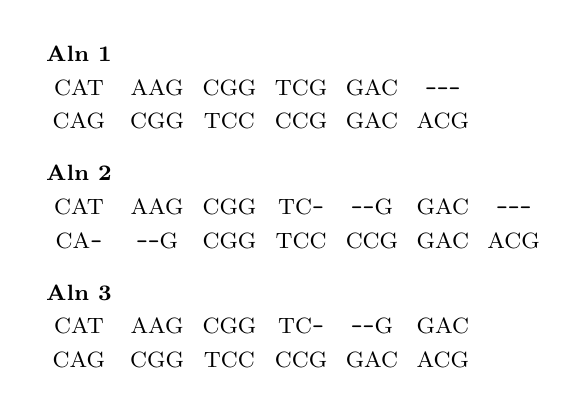
\begin{tikzpicture}[node distance=5mm,font=\footnotesize]
\tikzstyle{aln}=[matrix of nodes, nodes in empty cells]

\matrix (aln1)[aln] {
 \textbf{Aln 1} & & & & & &\\
CAT & AAG & CGG & TCG & GAC & \verb|---| &\\
CAG & CGG & TCC & CCG & GAC & ACG &\\
\\
 \textbf{Aln 2} & & & & & &\\
CAT & AAG & CGG & TC\verb|-| & \verb|--|G & GAC & \verb|---|\\
CA\verb|-| & \verb|--|G & CGG & TCC & CCG & GAC & ACG\\
\\
 \textbf{Aln 3} & & & & & &\\
CAT & AAG & CGG & TC\verb|-| & \verb|--|G & GAC &\\
CAG & CGG & TCC & CCG & GAC & ACG &\\
};
\end{tikzpicture}}
%     \column{0.6\textwidth}
%         % \resizebox{\textheight}{!}{\input{figures/alndotplot/example-expanded}}
%         \resizebox{\textheight}{!}{% Created by tikzDevice version 0.12.5 on 2023-10-08 01:40:20
% !TEX encoding = UTF-8 Unicode
\definecolor{color1}{HTML}{CC9966}
\definecolor{color2}{HTML}{99CCFF}
\definecolor{viridis0}{RGB}{255, 255, 255}
\definecolor{viridis1}{RGB}{253, 231, 37}
\definecolor{viridis2}{RGB}{181, 222, 43}
\definecolor{viridis3}{RGB}{110, 206, 88}
\definecolor{viridis4}{RGB}{53, 183, 121}
\definecolor{viridis5}{RGB}{31, 158, 137}
\definecolor{viridis6}{RGB}{38, 130, 142}
\definecolor{viridis7}{RGB}{49, 104, 142}
\definecolor{viridis8}{RGB}{62, 73, 137}
\definecolor{viridis9}{RGB}{72, 40, 120}
\definecolor{viridis10}{RGB}{68, 1, 84}
\begin{tikzpicture}[box/.style={rectangle, minimum size=0.5cm}]
\draw[very thin, color = gray!50, step = 0.5] (0,0) grid (19, 16);
\node at (0.25,15.25) {-};
\node at (0.25,14.75) {C};
\node at (0.25,14.25) {-};
\node at (0.25,13.75) {A};
\node at (0.25,13.25) {-};
\node at (0.25,12.75) {T};
\node at (0.25,12.25) {-};
\node at (0.25,11.75) {A};
\node at (0.25,11.25) {-};
\node at (0.25,10.75) {A};
\node at (0.25,10.25) {-};
\node at (0.25,9.75) {G};
\node at (0.25,9.25) {-};
\node at (0.25,8.75) {C};
\node at (0.25,8.25) {-};
\node at (0.25,7.75) {G};
\node at (0.25,7.25) {-};
\node at (0.25,6.75) {G};
\node at (0.25,6.25) {-};
\node at (0.25,5.75) {T};
\node at (0.25,5.25) {-};
\node at (0.25,4.75) {C};
\node at (0.25,4.25) {-};
\node at (0.25,3.75) {G};
\node at (0.25,3.25) {-};
\node at (0.25,2.75) {G};
\node at (0.25,2.25) {-};
\node at (0.25,1.75) {A};
\node at (0.25,1.25) {-};
\node at (0.25,0.75) {C};
\node at (0.25,0.25) {-};
\node at (0.75,15.75) {-};
\node at (1.25,15.75) {C};
\node at (1.75,15.75) {-};
\node at (2.25,15.75) {A};
\node at (2.75,15.75) {-};
\node at (3.25,15.75) {G};
\node at (3.75,15.75) {-};
\node at (4.25,15.75) {C};
\node at (4.75,15.75) {-};
\node at (5.25,15.75) {G};
\node at (5.75,15.75) {-};
\node at (6.25,15.75) {G};
\node at (6.75,15.75) {-};
\node at (7.25,15.75) {T};
\node at (7.75,15.75) {-};
\node at (8.25,15.75) {C};
\node at (8.75,15.75) {-};
\node at (9.25,15.75) {C};
\node at (9.75,15.75) {-};
\node at (10.25,15.75) {C};
\node at (10.75,15.75) {-};
\node at (11.25,15.75) {C};
\node at (11.75,15.75) {-};
\node at (12.25,15.75) {G};
\node at (12.75,15.75) {-};
\node at (13.25,15.75) {G};
\node at (13.75,15.75) {-};
\node at (14.25,15.75) {A};
\node at (14.75,15.75) {-};
\node at (15.25,15.75) {C};
\node at (15.75,15.75) {-};
\node at (16.25,15.75) {A};
\node at (16.75,15.75) {-};
\node at (17.25,15.75) {C};
\node at (17.75,15.75) {-};
\node at (18.25,15.75) {G};
\node at (18.75,15.75) {-};
\node[box, fill=viridis10] at (0.75, 15.25){};
\node[box, fill=viridis10] at (1.25, 14.75){};
\node[box, fill=viridis10] at (1.75, 14.25){};
\node[box, fill=viridis10] at (2.25, 13.75){};
\node[box, fill=viridis10] at (2.75, 13.25){};
\node[box, fill=viridis4] at (2.75, 12.75){};
\node[box, fill=viridis7] at (3.25, 12.75){};
\node[box, fill=viridis4] at (2.75, 12.25){};
\node[box, fill=viridis7] at (3.75, 12.25){};
\node[box, fill=viridis4] at (2.75, 11.75){};
\node[box, fill=viridis7] at (4.25, 11.75){};
\node[box, fill=viridis4] at (2.75, 11.25){};
\node[box, fill=viridis7] at (4.75, 11.25){};
\node[box, fill=viridis4] at (2.75, 10.75){};
\node[box, fill=viridis7] at (5.25, 10.75){};
\node[box, fill=viridis4] at (2.75, 10.25){};
\node[box, fill=viridis7] at (5.75, 10.25){};
\node[box, fill=viridis4] at (3.25, 9.75){};
\node[box, fill=viridis7] at (6.25, 9.75){};
\node[box, fill=viridis4] at (3.75, 9.25){};
\node[box, fill=viridis7] at (6.75, 9.25){};
\node[box, fill=viridis4] at (4.25, 8.75){};
\node[box, fill=viridis7] at (7.25, 8.75){};
\node[box, fill=viridis4] at (4.75, 8.25){};
\node[box, fill=viridis7] at (7.75, 8.25){};
\node[box, fill=viridis4] at (5.25, 7.75){};
\node[box, fill=viridis7] at (8.25, 7.75){};
\node[box, fill=viridis4] at (5.75, 7.25){};
\node[box, fill=viridis7] at (8.75, 7.25){};
\node[box, fill=viridis4] at (6.25, 6.75){};
\node[box, fill=viridis7] at (9.25, 6.75){};
\node[box, fill=viridis4] at (6.75, 6.25){};
\node[box, fill=viridis7] at (9.75, 6.25){};
\node[box, fill=viridis4] at (7.25, 5.75){};
\node[box, fill=viridis7] at (10.25, 5.75){};
\node[box, fill=viridis4] at (7.75, 5.25){};
\node[box, fill=viridis7] at (10.75, 5.25){};
\node[box, fill=viridis4] at (8.25, 4.75){};
\node[box, fill=viridis7] at (11.25, 4.75){};
\node[box, fill=viridis4] at (8.75, 4.25){};
\node[box, fill=viridis4] at (9.25, 4.25){};
\node[box, fill=viridis4] at (9.75, 4.25){};
\node[box, fill=viridis4] at (10.25, 4.25){};
\node[box, fill=viridis4] at (10.75, 4.25){};
\node[box, fill=viridis4] at (11.25, 4.25){};
\node[box, fill=viridis10] at (11.75, 4.25){};
\node[box, fill=viridis4] at (12.25, 4.25){};
\node[box, fill=viridis4] at (12.75, 4.25){};
\node[box, fill=viridis4] at (13.25, 4.25){};
\node[box, fill=viridis4] at (13.75, 4.25){};
\node[box, fill=viridis4] at (14.25, 4.25){};
\node[box, fill=viridis4] at (14.75, 4.25){};
\node[box, fill=viridis7] at (12.25, 3.75){};
\node[box, fill=viridis4] at (15.25, 3.75){};
\node[box, fill=viridis7] at (12.75, 3.25){};
\node[box, fill=viridis4] at (15.75, 3.25){};
\node[box, fill=viridis7] at (13.25, 2.75){};
\node[box, fill=viridis4] at (16.25, 2.75){};
\node[box, fill=viridis7] at (13.75, 2.25){};
\node[box, fill=viridis4] at (16.75, 2.25){};
\node[box, fill=viridis7] at (14.25, 1.75){};
\node[box, fill=viridis4] at (17.25, 1.75){};
\node[box, fill=viridis7] at (14.75, 1.25){};
\node[box, fill=viridis4] at (17.75, 1.25){};
\node[box, fill=viridis7] at (15.25, 0.75){};
\node[box, fill=viridis4] at (18.25, 0.75){};
\node[box, fill=viridis7] at (15.75, 0.25){};
\node[box, fill=viridis7] at (16.25, 0.25){};
\node[box, fill=viridis7] at (16.75, 0.25){};
\node[box, fill=viridis7] at (17.25, 0.25){};
\node[box, fill=viridis7] at (17.75, 0.25){};
\node[box, fill=viridis7] at (18.25, 0.25){};
\node[box, fill=viridis10] at (18.75, 0.25){};
\matrix [draw, below right, draw=none] at (current bounding box.north east) {
        % \node[box, fill=viridis0, scale=0.75] {0\%}; \\
        \node[box, fill=viridis1, scale=0.75] {00-09\%}; \\
        \node[box, fill=viridis2, scale=0.75] {10-19\%}; \\
        \node[box, fill=viridis3, scale=0.75] {20-29\%}; \\
        \node[box, fill=viridis4, scale=0.75] {30-29\%}; \\
        \node[box, fill=viridis5, scale=0.75] {\textcolor{white}{40-49\%}}; \\
        \node[box, fill=viridis6, scale=0.75] {\textcolor{white}{50-59\%}}; \\
        \node[box, fill=viridis7, scale=0.75] {\textcolor{white}{60-69\%}}; \\
        \node[box, fill=viridis8, scale=0.75] {\textcolor{white}{70-79\%}}; \\
        \node[box, fill=viridis9, scale=0.75] {\textcolor{white}{80-89\%}}; \\
        \node[box, fill=viridis10, scale=0.75] {\textcolor{white}{90-100\%}}; \\
    };
\end{tikzpicture}
}
% \end{columns}
% \end{frame} %-------------------------------------------------------------------

% \begin{frame}{Line} %-----------------------------------------------------------
% \begin{columns}
%     \column{0.4\textwidth}
%         Lines display more information when paths cross but can't identify full paths.\\
%         \vspace{1em}
%         \resizebox{!}{0.5\textwidth}{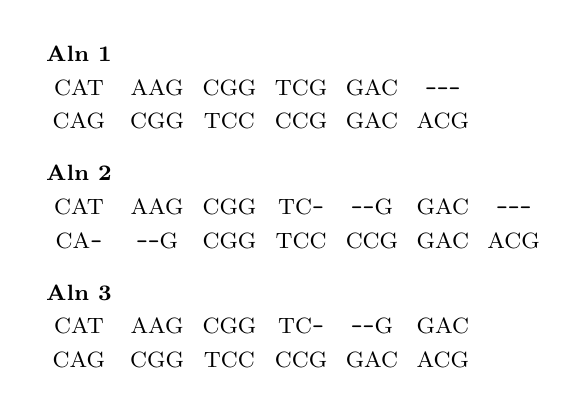
\begin{tikzpicture}[node distance=5mm,font=\footnotesize]
\tikzstyle{aln}=[matrix of nodes, nodes in empty cells]

\matrix (aln1)[aln] {
 \textbf{Aln 1} & & & & & &\\
CAT & AAG & CGG & TCG & GAC & \verb|---| &\\
CAG & CGG & TCC & CCG & GAC & ACG &\\
\\
 \textbf{Aln 2} & & & & & &\\
CAT & AAG & CGG & TC\verb|-| & \verb|--|G & GAC & \verb|---|\\
CA\verb|-| & \verb|--|G & CGG & TCC & CCG & GAC & ACG\\
\\
 \textbf{Aln 3} & & & & & &\\
CAT & AAG & CGG & TC\verb|-| & \verb|--|G & GAC &\\
CAG & CGG & TCC & CCG & GAC & ACG &\\
};
\end{tikzpicture}}
%     \column{0.6\textwidth}
%         \centering
%         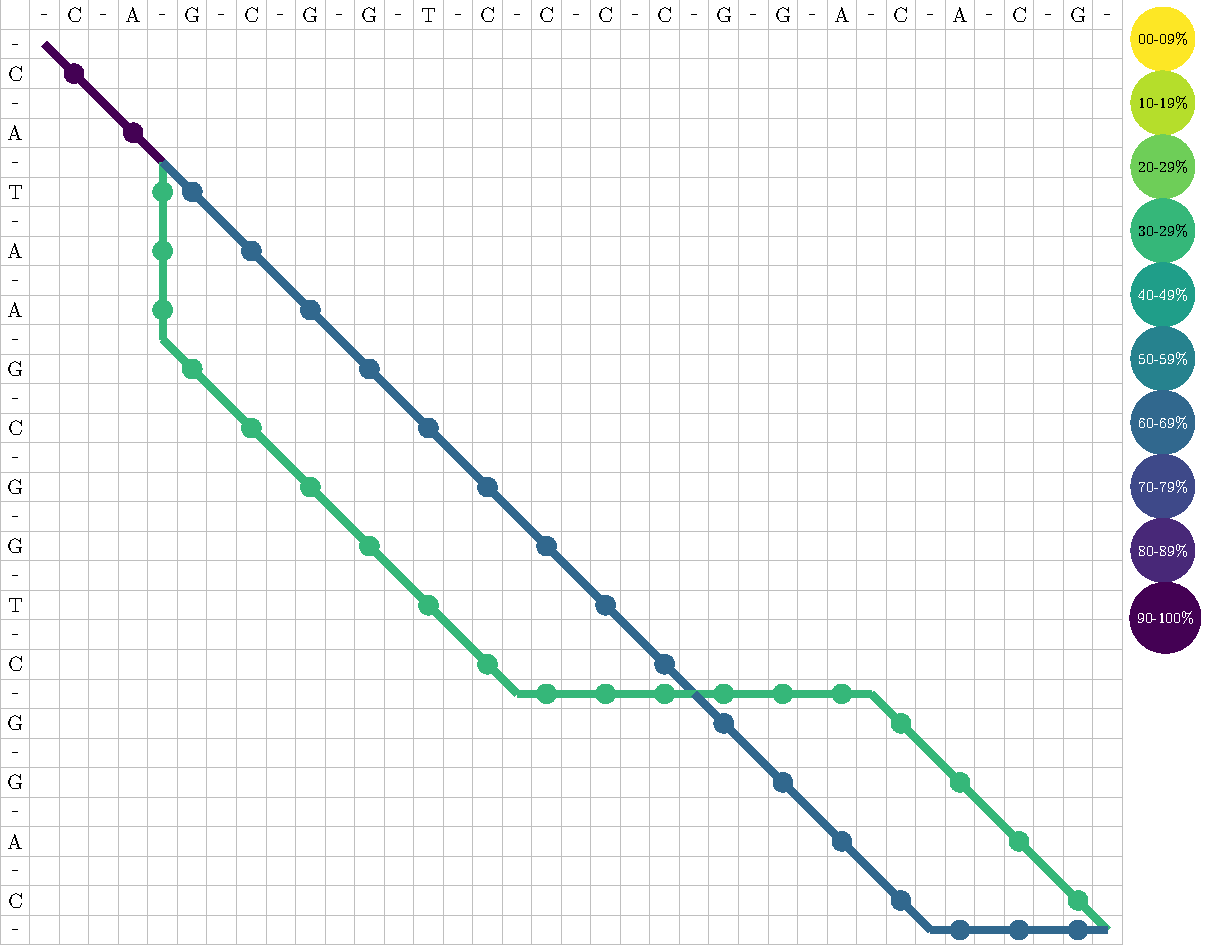
\includegraphics[height = 0.8\textheight]{defense/figures/alndotplot/example-line.pdf}
%         % \resizebox{\textheight}{!}{\definecolor{color1}{HTML}{CC9966}
\definecolor{color2}{HTML}{99CCFF}
\definecolor{viridis0}{RGB}{255, 255, 255}
\definecolor{viridis1}{RGB}{253, 231, 37}
\definecolor{viridis2}{RGB}{181, 222, 43}
\definecolor{viridis3}{RGB}{110, 206, 88}
\definecolor{viridis4}{RGB}{53, 183, 121}
\definecolor{viridis5}{RGB}{31, 158, 137}
\definecolor{viridis6}{RGB}{38, 130, 142}
\definecolor{viridis7}{RGB}{49, 104, 142}
\definecolor{viridis8}{RGB}{62, 73, 137}
\definecolor{viridis9}{RGB}{72, 40, 120}
\definecolor{viridis10}{RGB}{68, 1, 84}
\begin{tikzpicture}[dot/.style={circle, minimum size=2.5mm}]
\draw[very thin, color = gray!50, step = 0.5] (0,0) grid (19, 16);
\node at (0.25,15.25) {-};
\node at (0.25,14.75) {C};
\node at (0.25,14.25) {-};
\node at (0.25,13.75) {A};
\node at (0.25,13.25) {-};
\node at (0.25,12.75) {T};
\node at (0.25,12.25) {-};
\node at (0.25,11.75) {A};
\node at (0.25,11.25) {-};
\node at (0.25,10.75) {A};
\node at (0.25,10.25) {-};
\node at (0.25,9.75) {G};
\node at (0.25,9.25) {-};
\node at (0.25,8.75) {C};
\node at (0.25,8.25) {-};
\node at (0.25,7.75) {G};
\node at (0.25,7.25) {-};
\node at (0.25,6.75) {G};
\node at (0.25,6.25) {-};
\node at (0.25,5.75) {T};
\node at (0.25,5.25) {-};
\node at (0.25,4.75) {C};
\node at (0.25,4.25) {-};
\node at (0.25,3.75) {G};
\node at (0.25,3.25) {-};
\node at (0.25,2.75) {G};
\node at (0.25,2.25) {-};
\node at (0.25,1.75) {A};
\node at (0.25,1.25) {-};
\node at (0.25,0.75) {C};
\node at (0.25,0.25) {-};
\node at (0.75,15.75) {-};
\node at (1.25,15.75) {C};
\node at (1.75,15.75) {-};
\node at (2.25,15.75) {A};
\node at (2.75,15.75) {-};
\node at (3.25,15.75) {G};
\node at (3.75,15.75) {-};
\node at (4.25,15.75) {C};
\node at (4.75,15.75) {-};
\node at (5.25,15.75) {G};
\node at (5.75,15.75) {-};
\node at (6.25,15.75) {G};
\node at (6.75,15.75) {-};
\node at (7.25,15.75) {T};
\node at (7.75,15.75) {-};
\node at (8.25,15.75) {C};
\node at (8.75,15.75) {-};
\node at (9.25,15.75) {C};
\node at (9.75,15.75) {-};
\node at (10.25,15.75) {C};
\node at (10.75,15.75) {-};
\node at (11.25,15.75) {C};
\node at (11.75,15.75) {-};
\node at (12.25,15.75) {G};
\node at (12.75,15.75) {-};
\node at (13.25,15.75) {G};
\node at (13.75,15.75) {-};
\node at (14.25,15.75) {A};
\node at (14.75,15.75) {-};
\node at (15.25,15.75) {C};
\node at (15.75,15.75) {-};
\node at (16.25,15.75) {A};
\node at (16.75,15.75) {-};
\node at (17.25,15.75) {C};
\node at (17.75,15.75) {-};
\node at (18.25,15.75) {G};
\node at (18.75,15.75) {-};
\draw[line width=1.25mm,viridis10](0.75,15.25)--(1.25,14.75);
\draw[line width=1.25mm,viridis10](1.25,14.75)--(1.75,14.25);
\node[circle, fill=viridis10] at (1.25, 14.75){};
\draw[line width=1.25mm,viridis10](1.75,14.25)--(2.25,13.75);
\draw[line width=1.25mm,viridis10](2.25,13.75)--(2.75,13.25);
\node[circle, fill=viridis10] at (2.25, 13.75){};
\draw[line width=1.25mm,viridis4](2.75,13.25)--(2.75,12.75);
\draw[line width=1.25mm,viridis7](2.75,13.25)--(3.25,12.75);
\draw[line width=1.25mm,viridis4](2.75,12.75)--(2.75,12.25);
\node[circle, fill=viridis4] at (2.75, 12.75){};
\draw[line width=1.25mm,viridis7](3.25,12.75)--(3.75,12.25);
\node[circle, fill=viridis7] at (3.25, 12.75){};
\draw[line width=1.25mm,viridis4](2.75,12.25)--(2.75,11.75);
\draw[line width=1.25mm,viridis7](3.75,12.25)--(4.25,11.75);
\draw[line width=1.25mm,viridis4](2.75,11.75)--(2.75,11.25);
\node[circle, fill=viridis4] at (2.75, 11.75){};
\draw[line width=1.25mm,viridis7](4.25,11.75)--(4.75,11.25);
\node[circle, fill=viridis7] at (4.25, 11.75){};
\draw[line width=1.25mm,viridis4](2.75,11.25)--(2.75,10.75);
\draw[line width=1.25mm,viridis7](4.75,11.25)--(5.25,10.75);
\draw[line width=1.25mm,viridis4](2.75,10.75)--(2.75,10.25);
\node[circle, fill=viridis4] at (2.75, 10.75){};
\draw[line width=1.25mm,viridis7](5.25,10.75)--(5.75,10.25);
\node[circle, fill=viridis7] at (5.25, 10.75){};
\draw[line width=1.25mm,viridis4](2.75,10.25)--(3.25,9.75);
\draw[line width=1.25mm,viridis7](5.75,10.25)--(6.25,9.75);
\draw[line width=1.25mm,viridis4](3.25,9.75)--(3.75,9.25);
\node[circle, fill=viridis4] at (3.25, 9.75){};
\draw[line width=1.25mm,viridis7](6.25,9.75)--(6.75,9.25);
\node[circle, fill=viridis7] at (6.25, 9.75){};
\draw[line width=1.25mm,viridis4](3.75,9.25)--(4.25,8.75);
\draw[line width=1.25mm,viridis7](6.75,9.25)--(7.25,8.75);
\draw[line width=1.25mm,viridis4](4.25,8.75)--(4.75,8.25);
\node[circle, fill=viridis4] at (4.25, 8.75){};
\draw[line width=1.25mm,viridis7](7.25,8.75)--(7.75,8.25);
\node[circle, fill=viridis7] at (7.25, 8.75){};
\draw[line width=1.25mm,viridis4](4.75,8.25)--(5.25,7.75);
\draw[line width=1.25mm,viridis7](7.75,8.25)--(8.25,7.75);
\draw[line width=1.25mm,viridis4](5.25,7.75)--(5.75,7.25);
\node[circle, fill=viridis4] at (5.25, 7.75){};
\draw[line width=1.25mm,viridis7](8.25,7.75)--(8.75,7.25);
\node[circle, fill=viridis7] at (8.25, 7.75){};
\draw[line width=1.25mm,viridis4](5.75,7.25)--(6.25,6.75);
\draw[line width=1.25mm,viridis7](8.75,7.25)--(9.25,6.75);
\draw[line width=1.25mm,viridis4](6.25,6.75)--(6.75,6.25);
\node[circle, fill=viridis4] at (6.25, 6.75){};
\draw[line width=1.25mm,viridis7](9.25,6.75)--(9.75,6.25);
\node[circle, fill=viridis7] at (9.25, 6.75){};
\draw[line width=1.25mm,viridis4](6.75,6.25)--(7.25,5.75);
\draw[line width=1.25mm,viridis7](9.75,6.25)--(10.25,5.75);
\draw[line width=1.25mm,viridis4](7.25,5.75)--(7.75,5.25);
\node[circle, fill=viridis4] at (7.25, 5.75){};
\draw[line width=1.25mm,viridis7](10.25,5.75)--(10.75,5.25);
\node[circle, fill=viridis7] at (10.25, 5.75){};
\draw[line width=1.25mm,viridis4](7.75,5.25)--(8.25,4.75);
\draw[line width=1.25mm,viridis7](10.75,5.25)--(11.25,4.75);
\draw[line width=1.25mm,viridis4](8.25,4.75)--(8.75,4.25);
\node[circle, fill=viridis4] at (8.25, 4.75){};
\draw[line width=1.25mm,viridis7](11.25,4.75)--(11.75,4.25);
\node[circle, fill=viridis7] at (11.25, 4.75){};
\draw[line width=1.25mm,viridis4](8.75,4.25)--(9.25,4.25);
\draw[line width=1.25mm,viridis4](9.25,4.25)--(9.75,4.25);
\node[circle, fill=viridis4] at (9.25, 4.25){};
\draw[line width=1.25mm,viridis4](9.75,4.25)--(10.25,4.25);
\draw[line width=1.25mm,viridis4](10.25,4.25)--(10.75,4.25);
\node[circle, fill=viridis4] at (10.25, 4.25){};
\draw[line width=1.25mm,viridis4](10.75,4.25)--(11.25,4.25);
\draw[line width=1.25mm,viridis4](11.25,4.25)--(11.75,4.25);
\node[circle, fill=viridis4] at (11.25, 4.25){};
\draw[line width=1.25mm,viridis4](11.75,4.25)--(12.25,4.25);
\draw[line width=1.25mm,viridis7](11.75,4.25)--(12.25,3.75);
\draw[line width=1.25mm,viridis4](12.25,4.25)--(12.75,4.25);
\node[circle, fill=viridis4] at (12.25, 4.25){};
\draw[line width=1.25mm,viridis4](12.75,4.25)--(13.25,4.25);
\draw[line width=1.25mm,viridis4](13.25,4.25)--(13.75,4.25);
\node[circle, fill=viridis4] at (13.25, 4.25){};
\draw[line width=1.25mm,viridis4](13.75,4.25)--(14.25,4.25);
\draw[line width=1.25mm,viridis4](14.25,4.25)--(14.75,4.25);
\node[circle, fill=viridis4] at (14.25, 4.25){};
\draw[line width=1.25mm,viridis4](14.75,4.25)--(15.25,3.75);
\draw[line width=1.25mm,viridis7](12.25,3.75)--(12.75,3.25);
\node[circle, fill=viridis7] at (12.25, 3.75){};
\draw[line width=1.25mm,viridis4](15.25,3.75)--(15.75,3.25);
\node[circle, fill=viridis4] at (15.25, 3.75){};
\draw[line width=1.25mm,viridis7](12.75,3.25)--(13.25,2.75);
\draw[line width=1.25mm,viridis4](15.75,3.25)--(16.25,2.75);
\draw[line width=1.25mm,viridis7](13.25,2.75)--(13.75,2.25);
\node[circle, fill=viridis7] at (13.25, 2.75){};
\draw[line width=1.25mm,viridis4](16.25,2.75)--(16.75,2.25);
\node[circle, fill=viridis4] at (16.25, 2.75){};
\draw[line width=1.25mm,viridis7](13.75,2.25)--(14.25,1.75);
\draw[line width=1.25mm,viridis4](16.75,2.25)--(17.25,1.75);
\draw[line width=1.25mm,viridis7](14.25,1.75)--(14.75,1.25);
\node[circle, fill=viridis7] at (14.25, 1.75){};
\draw[line width=1.25mm,viridis4](17.25,1.75)--(17.75,1.25);
\node[circle, fill=viridis4] at (17.25, 1.75){};
\draw[line width=1.25mm,viridis7](14.75,1.25)--(15.25,0.75);
\draw[line width=1.25mm,viridis4](17.75,1.25)--(18.25,0.75);
\draw[line width=1.25mm,viridis7](15.25,0.75)--(15.75,0.25);
\node[circle, fill=viridis7] at (15.25, 0.75){};
\draw[line width=1.25mm,viridis4](18.25,0.75)--(18.75,0.25);
\node[circle, fill=viridis4] at (18.25, 0.75){};
\draw[line width=1.25mm,viridis7](15.75,0.25)--(16.25,0.25);
\draw[line width=1.25mm,viridis7](16.25,0.25)--(16.75,0.25);
\node[circle, fill=viridis7] at (16.25, 0.25){};
\draw[line width=1.25mm,viridis7](16.75,0.25)--(17.25,0.25);
\draw[line width=1.25mm,viridis7](17.25,0.25)--(17.75,0.25);
\node[circle, fill=viridis7] at (17.25, 0.25){};
\draw[line width=1.25mm,viridis7](17.75,0.25)--(18.25,0.25);
\draw[line width=1.25mm,viridis7](18.25,0.25)--(18.75,0.25);
\node[circle, fill=viridis7] at (18.25, 0.25){};
\matrix [draw, below right, draw=none] at (current bounding box.north east) {
        % \node[circle, fill=viridis0, scale=0.75] {0\%}; \\
        \node[circle, fill=viridis1, scale=0.75] {00-09\%}; \\
        \node[circle, fill=viridis2, scale=0.75] {10-19\%}; \\
        \node[circle, fill=viridis3, scale=0.75] {20-29\%}; \\
        \node[circle, fill=viridis4, scale=0.75] {30-29\%}; \\
        \node[circle, fill=viridis5, scale=0.75] {\textcolor{white}{40-49\%}}; \\
        \node[circle, fill=viridis6, scale=0.75] {\textcolor{white}{50-59\%}}; \\
        \node[circle, fill=viridis7, scale=0.75] {\textcolor{white}{60-69\%}}; \\
        \node[circle, fill=viridis8, scale=0.75] {\textcolor{white}{70-79\%}}; \\
        \node[circle, fill=viridis9, scale=0.75] {\textcolor{white}{80-89\%}}; \\
        \node[circle, fill=viridis10, scale=0.75] {\textcolor{white}{90-100\%}}; \\
    };
\end{tikzpicture}
}
% \end{columns}
% \note[item]{Helps when multiple paths are close together (e.g. intersection). Clarifies how many com from where (more helpful with more alignments).}
% \end{frame} %-------------------------------------------------------------------

\begin{frame}[c]{Multiple Lines} %------------------------------------------------
\begin{columns}
    \column{0.4\textwidth}
        \centering
        \definecolor{color1}{HTML}{CC9966}
\definecolor{color2}{HTML}{99CCFF}
\definecolor{color3}{HTML}{77DD77}

\begin{tikzpicture}[node distance=5mm,font=\footnotesize]
\tikzstyle{aln}=[matrix of nodes, nodes in empty cells]

\matrix (aln1)[aln] {
 \textbf{\textcolor{color1}{Aln 1}} & & &\\
CAT & \verb|---| & AAG &\\
C\verb|-|G & CGG & ACG &\\
\\
 \textbf{\textcolor{color2}{Aln 2}} & & &\\
CAT & \verb|--|A & A\verb|-|G &\\
CG\verb|-| & CGG & ACG &\\
\\
 \textbf{\textcolor{color3}{Aln 3}} & & &\\
CAT & \verb|--|A & A\verb|-|G &\\
CGC & GGA & \verb|-|CG &\\
};
\end{tikzpicture}
    \column{0.6\textwidth}
        \centering
        \resizebox{\textwidth}{!}{% Created by tikzDevice version 0.12.5 on 2023-10-23 23:03:40
% !TEX encoding = UTF-8 Unicode
\definecolor{color1}{HTML}{CC9966}
\definecolor{color2}{HTML}{99CCFF}
\definecolor{color3}{HTML}{77DD77}

\begin{tikzpicture}[dot/.style={circle,scale=1.5, minimum size=1cm, inner sep=0pt, outer sep=0pt}]
\draw[very thin, color = gray!50, step = 1.5] (0,0) grid (27, 21);
\node [scale=2.5] at (0.75,18.75) {-};
\node [scale=2.5] at (0.75,17.25) {C};
\node [scale=2.5] at (0.75,15.75) {-};
\node [scale=2.5] at (0.75,14.25) {A};
\node [scale=2.5] at (0.75,12.75) {-};
\node [scale=2.5] at (0.75,11.25) {T};
\node [scale=2.5] at (0.75,9.75) {-};
\node [scale=2.5] at (0.75,8.25) {A};
\node [scale=2.5] at (0.75,6.75) {-};
\node [scale=2.5] at (0.75,5.25) {A};
\node [scale=2.5] at (0.75,3.75) {-};
\node [scale=2.5] at (0.75,2.25) {G};
\node [scale=2.5] at (0.75,0.75) {-};
\node [scale=2.5] at (2.25,20.25) {-};
\node [scale=2.5] at (3.75,20.25) {C};
\node [scale=2.5] at (5.25,20.25) {-};
\node [scale=2.5] at (6.75,20.25) {G};
\node [scale=2.5] at (8.25,20.25) {-};
\node [scale=2.5] at (9.75,20.25) {C};
\node [scale=2.5] at (11.25,20.25) {-};
\node [scale=2.5] at (12.75,20.25) {G};
\node [scale=2.5] at (14.25,20.25) {-};
\node [scale=2.5] at (15.75,20.25) {G};
\node [scale=2.5] at (17.25,20.25) {-};
\node [scale=2.5] at (18.75,20.25) {A};
\node [scale=2.5] at (20.25,20.25) {-};
\node [scale=2.5] at (21.75,20.25) {C};
\node [scale=2.5] at (23.25,20.25) {-};
\node [scale=2.5] at (24.75,20.25) {G};
\node [scale=2.5] at (26.25,20.25) {-};
\draw[line width=1.875mm,color1](1.75,18.25)--(3.25,16.75);
\draw[line width=1.875mm,color1](3.25,16.75)--(4.75,15.25);
\node[circle,scale=1.5, fill=color1] at (3.25, 16.75){};
\node[black,scale=1.5] at (3.25, 16.75){$\mathlarger{\mathlarger{\bm{\times}}}$};
\draw[line width=1.875mm,color1](4.75,15.25)--(4.75,13.75);
\draw[line width=1.875mm,color1](4.75,13.75)--(4.75,12.25);
\node[circle,scale=1.5, fill=color1] at (4.75, 13.75){};
\draw[line width=1.875mm,color1](4.75,12.25)--(6.25,10.75);
\draw[line width=1.875mm,color1](6.25,10.75)--(7.75,9.25);
\node[circle,scale=1.5, fill=color1] at (6.25, 10.75){};
\draw[line width=1.875mm,color1](7.75,9.25)--(9.25,9.25);
\draw[line width=1.875mm,color1](9.25,9.25)--(10.75,9.25);
\node[circle,scale=1.5, fill=color1] at (9.25, 9.25){};
\draw[line width=1.875mm,color1](10.75,9.25)--(12.25,9.25);
\draw[line width=1.875mm,color1](12.25,9.25)--(13.75,9.25);
\node[circle,scale=1.5, fill=color1] at (12.25, 9.25){};
\draw[line width=1.875mm,color1](13.75,9.25)--(15.25,9.25);
\draw[line width=1.875mm,color1](15.25,9.25)--(16.75,9.25);
\node[circle,scale=1.5, fill=color1] at (15.25, 9.25){};
\draw[line width=1.875mm,color1](16.75,9.25)--(18.25,7.75);
\draw[line width=1.875mm,color1](18.25,7.75)--(19.75,6.25);
\node[circle,scale=1.5, fill=color1] at (18.25, 7.75){};
\node[black,scale=1.5] at (18.25, 7.75){$\mathlarger{\mathlarger{\bm{\times}}}$};
\draw[line width=1.875mm,color1](19.75,6.25)--(21.25,4.75);
\draw[line width=1.875mm,color1](21.25,4.75)--(22.75,3.25);
\node[circle,scale=1.5, fill=color1] at (21.25, 4.75){};
\draw[line width=1.875mm,color1](22.75,3.25)--(24.25,1.75);
\draw[line width=1.875mm,color1](24.25,1.75)--(25.75,0.25);
\node[circle,scale=1.5, fill=color1] at (24.25, 1.75){};
\node[black,scale=1.5] at (24.25, 1.75){$\mathlarger{\mathlarger{\bm{\times}}}$};
\draw[line width=1.875mm,color2](2.25,18.75)--(3.75,17.25);
\draw[line width=1.875mm,color2](3.75,17.25)--(5.25,15.75);
\node[circle,scale=1.5, fill=color2] at (3.75, 17.25){};
\node[black,scale=1.5] at (3.75, 17.25){$\mathlarger{\mathlarger{\bm{\times}}}$};
\draw[line width=1.875mm,color2](5.25,15.75)--(6.75,14.25);
\draw[line width=1.875mm,color2](6.75,14.25)--(8.25,12.75);
\node[circle,scale=1.5, fill=color2] at (6.75, 14.25){};
\draw[line width=1.875mm,color2](8.25,12.75)--(8.25,11.25);
\draw[line width=1.875mm,color2](8.25,11.25)--(8.25,9.75);
\node[circle,scale=1.5, fill=color2] at (8.25, 11.25){};
\draw[line width=1.875mm,color2](8.25,9.75)--(9.75,9.75);
\draw[line width=1.875mm,color2](9.75,9.75)--(11.25,9.75);
\node[circle,scale=1.5, fill=color2] at (9.75, 9.75){};
\draw[line width=1.875mm,color2](11.25,9.75)--(12.75,9.75);
\draw[line width=1.875mm,color2](12.75,9.75)--(14.25,9.75);
\node[circle,scale=1.5, fill=color2] at (12.75, 9.75){};
\draw[line width=1.875mm,color2](14.25,9.75)--(15.75,8.25);
\draw[line width=1.875mm,color2](15.75,8.25)--(17.25,6.75);
\node[circle,scale=1.5, fill=color2] at (15.75, 8.25){};
\draw[line width=1.875mm,color2](17.25,6.75)--(18.75,5.25);
\draw[line width=1.875mm,color2](18.75,5.25)--(20.25,3.75);
\node[circle,scale=1.5, fill=color2] at (18.75, 5.25){};
\node[black,scale=1.5] at (18.75, 5.25){$\mathlarger{\mathlarger{\bm{\times}}}$};
\draw[line width=1.875mm,color2](20.25,3.75)--(21.75,3.75);
\draw[line width=1.875mm,color2](21.75,3.75)--(23.25,3.75);
\node[circle,scale=1.5, fill=color2] at (21.75, 3.75){};
\draw[line width=1.875mm,color2](23.25,3.75)--(24.75,2.25);
\draw[line width=1.875mm,color2](24.75,2.25)--(26.25,0.75);
\node[circle,scale=1.5, fill=color2] at (24.75, 2.25){};
\node[black,scale=1.5] at (24.75, 2.25){$\mathlarger{\mathlarger{\bm{\times}}}$};
\draw[line width=1.875mm,color3](2.75,19.25)--(4.25,17.75);
\draw[line width=1.875mm,color3](4.25,17.75)--(5.75,16.25);
\node[circle,scale=1.5, fill=color3] at (4.25, 17.75){};
\node[black,scale=1.5] at (4.25, 17.75){$\mathlarger{\mathlarger{\bm{\times}}}$};
\draw[line width=1.875mm,color3](5.75,16.25)--(7.25,14.75);
\draw[line width=1.875mm,color3](7.25,14.75)--(8.75,13.25);
\node[circle,scale=1.5, fill=color3] at (7.25, 14.75){};
\draw[line width=1.875mm,color3](8.75,13.25)--(10.25,11.75);
\draw[line width=1.875mm,color3](10.25,11.75)--(11.75,10.25);
\node[circle,scale=1.5, fill=color3] at (10.25, 11.75){};
\draw[line width=1.875mm,color3](11.75,10.25)--(13.25,10.25);
\draw[line width=1.875mm,color3](13.25,10.25)--(14.75,10.25);
\node[circle,scale=1.5, fill=color3] at (13.25, 10.25){};
\draw[line width=1.875mm,color3](14.75,10.25)--(16.25,10.25);
\draw[line width=1.875mm,color3](16.25,10.25)--(17.75,10.25);
\node[circle,scale=1.5, fill=color3] at (16.25, 10.25){};
\draw[line width=1.875mm,color3](17.75,10.25)--(19.25,8.75);
\draw[line width=1.875mm,color3](19.25,8.75)--(20.75,7.25);
\node[circle,scale=1.5, fill=color3] at (19.25, 8.75){};
\node[black,scale=1.5] at (19.25, 8.75){$\mathlarger{\mathlarger{\bm{\times}}}$};
\draw[line width=1.875mm,color3](20.75,7.25)--(20.75,5.75);
\draw[line width=1.875mm,color3](20.75,5.75)--(20.75,4.25);
\node[circle,scale=1.5, fill=color3] at (20.75, 5.75){};
\draw[line width=1.875mm,color3](20.75,4.25)--(22.25,4.25);
\draw[line width=1.875mm,color3](22.25,4.25)--(23.75,4.25);
\node[circle,scale=1.5, fill=color3] at (22.25, 4.25){};
\draw[line width=1.875mm,color3](23.75,4.25)--(25.25,2.75);
\draw[line width=1.875mm,color3](25.25,2.75)--(26.75,1.25);
\node[circle,scale=1.5, fill=color3] at (25.25, 2.75){};
\node[black,scale=1.5] at (25.25, 2.75){$\mathlarger{\mathlarger{\bm{\times}}}$};
\matrix [draw, below right, draw=none] at (current bounding box.north east) {
        \node[circle, fill=color1, scale=0.75] {Alignment 1}; \\
        \node[circle, fill=color2, scale=0.75] {Alignment 2}; \\
        \node[circle, fill=color3, scale=0.75] {Alignment 3}; \\
    };
\end{tikzpicture}
}
\end{columns}
\note[item]{This version allows us to compare specific alignments.}
\note[item]{<describe figure>.}
\note[item]{Transition: however, <next slide>.}
\end{frame} %---------------------------------------------------------------------

% \begin{frame}{Multiple Lines} %-------------------------------------------------
% \begin{columns}
%     \column{0.4\textwidth}
%         Multiple lines display different paths.\\
%         \vspace{1em}
%         % \resizebox{!}{0.5\textwidth}{\input{figures/alndotplot/fig-alndotplot-alns}}
%         \resizebox{!}{0.5\textwidth}{\definecolor{color1}{HTML}{CC9966}
\definecolor{color2}{HTML}{99CCFF}
\definecolor{color3}{HTML}{77DD77}
\begin{tikzpicture}[node distance=5mm,font=\footnotesize]
\tikzstyle{aln}=[matrix of nodes, nodes in empty cells]

\matrix (aln1)[aln] {
 \textcolor{color1}{\textbf{Aln 1}} & & & & & &\\
CAT & AAG & CGG & TCG & GAC & \verb|---| &\\
CAG & CGG & TCC & CCG & GAC & ACG &\\
\\
 \textcolor{color2}{\textbf{Aln 2}} & & & & & &\\
CAT & AAG & CGG & TC\verb|-| & \verb|--|G & GAC & \verb|---|\\
CA\verb|-| & \verb|--|G & CGG & TCC & CCG & GAC & ACG\\
\\
 \textcolor{color3}{\textbf{Aln 3}} & & & & & &\\
CAT & AAG & CGG & TC\verb|-| & \verb|--|G & GAC &\\
CAG & CGG & TCC & CCG & GAC & ACG &\\
};
\end{tikzpicture}}
%     \column{0.6\textwidth}
%         % \resizebox{!}{0.68\textwidth}{\definecolor{color1}{HTML}{CC9966}
\definecolor{color2}{HTML}{99CCFF}
\definecolor{color3}{HTML}{77DD77}
\begin{tikzpicture}[dot/.style={circle, minimum size=8mm}]
\draw[very thin, color = gray!50, step = 1.5] (0,0) grid (57, 48);
\node [scale=2.5] at (0.75,45.75) {-};
\node [scale=2.5] at (0.75,44.25) {C};
\node [scale=2.5] at (0.75,42.75) {-};
\node [scale=2.5] at (0.75,41.25) {A};
\node [scale=2.5] at (0.75,39.75) {-};
\node [scale=2.5] at (0.75,38.25) {T};
\node [scale=2.5] at (0.75,36.75) {-};
\node [scale=2.5] at (0.75,35.25) {A};
\node [scale=2.5] at (0.75,33.75) {-};
\node [scale=2.5] at (0.75,32.25) {A};
\node [scale=2.5] at (0.75,30.75) {-};
\node [scale=2.5] at (0.75,29.25) {G};
\node [scale=2.5] at (0.75,27.75) {-};
\node [scale=2.5] at (0.75,26.25) {C};
\node [scale=2.5] at (0.75,24.75) {-};
\node [scale=2.5] at (0.75,23.25) {G};
\node [scale=2.5] at (0.75,21.75) {-};
\node [scale=2.5] at (0.75,20.25) {G};
\node [scale=2.5] at (0.75,18.75) {-};
\node [scale=2.5] at (0.75,17.25) {T};
\node [scale=2.5] at (0.75,15.75) {-};
\node [scale=2.5] at (0.75,14.25) {C};
\node [scale=2.5] at (0.75,12.75) {-};
\node [scale=2.5] at (0.75,11.25) {G};
\node [scale=2.5] at (0.75,9.75) {-};
\node [scale=2.5] at (0.75,8.25) {G};
\node [scale=2.5] at (0.75,6.75) {-};
\node [scale=2.5] at (0.75,5.25) {A};
\node [scale=2.5] at (0.75,3.75) {-};
\node [scale=2.5] at (0.75,2.25) {C};
\node [scale=2.5] at (0.75,0.75) {-};
\node [scale=2.5] at (2.25,47.25) {-};
\node [scale=2.5] at (3.75,47.25) {C};
\node [scale=2.5] at (5.25,47.25) {-};
\node [scale=2.5] at (6.75,47.25) {A};
\node [scale=2.5] at (8.25,47.25) {-};
\node [scale=2.5] at (9.75,47.25) {G};
\node [scale=2.5] at (11.25,47.25) {-};
\node [scale=2.5] at (12.75,47.25) {C};
\node [scale=2.5] at (14.25,47.25) {-};
\node [scale=2.5] at (15.75,47.25) {G};
\node [scale=2.5] at (17.25,47.25) {-};
\node [scale=2.5] at (18.75,47.25) {G};
\node [scale=2.5] at (20.25,47.25) {-};
\node [scale=2.5] at (21.75,47.25) {T};
\node [scale=2.5] at (23.25,47.25) {-};
\node [scale=2.5] at (24.75,47.25) {C};
\node [scale=2.5] at (26.25,47.25) {-};
\node [scale=2.5] at (27.75,47.25) {C};
\node [scale=2.5] at (29.25,47.25) {-};
\node [scale=2.5] at (30.75,47.25) {C};
\node [scale=2.5] at (32.25,47.25) {-};
\node [scale=2.5] at (33.75,47.25) {C};
\node [scale=2.5] at (35.25,47.25) {-};
\node [scale=2.5] at (36.75,47.25) {G};
\node [scale=2.5] at (38.25,47.25) {-};
\node [scale=2.5] at (39.75,47.25) {G};
\node [scale=2.5] at (41.25,47.25) {-};
\node [scale=2.5] at (42.75,47.25) {A};
\node [scale=2.5] at (44.25,47.25) {-};
\node [scale=2.5] at (45.75,47.25) {C};
\node [scale=2.5] at (47.25,47.25) {-};
\node [scale=2.5] at (48.75,47.25) {A};
\node [scale=2.5] at (50.25,47.25) {-};
\node [scale=2.5] at (51.75,47.25) {C};
\node [scale=2.5] at (53.25,47.25) {-};
\node [scale=2.5] at (54.75,47.25) {G};
\node [scale=2.5] at (56.25,47.25) {-};
\draw[line width=2.875mm,color3](1.75,45.25)--(3.25,43.75);
\draw[line width=2.875mm,color3](3.25,43.75)--(4.75,42.25);
\node[dot, fill=color3] at (3.25, 43.75){};
\draw[line width=2.875mm,color3](4.75,42.25)--(6.25,40.75);
\draw[line width=2.875mm,color3](6.25,40.75)--(7.75,39.25);
\node[dot, fill=color3] at (6.25, 40.75){};
\draw[line width=2.875mm,color3](7.75,39.25)--(9.25,37.75);
\draw[line width=2.875mm,color3](9.25,37.75)--(10.75,36.25);
\node[dot, fill=color3] at (9.25, 37.75){};
\draw[line width=2.875mm,color3](10.75,36.25)--(12.25,34.75);
\draw[line width=2.875mm,color3](12.25,34.75)--(13.75,33.25);
\node[dot, fill=color3] at (12.25, 34.75){};
\draw[line width=2.875mm,color3](13.75,33.25)--(15.25,31.75);
\draw[line width=2.875mm,color3](15.25,31.75)--(16.75,30.25);
\node[dot, fill=color3] at (15.25, 31.75){};
\draw[line width=2.875mm,color3](16.75,30.25)--(18.25,28.75);
\draw[line width=2.875mm,color3](18.25,28.75)--(19.75,27.25);
\node[dot, fill=color3] at (18.25, 28.75){};
\draw[line width=2.875mm,color3](19.75,27.25)--(21.25,25.75);
\draw[line width=2.875mm,color3](21.25,25.75)--(22.75,24.25);
\node[dot, fill=color3] at (21.25, 25.75){};
\draw[line width=2.875mm,color3](22.75,24.25)--(24.25,22.75);
\draw[line width=2.875mm,color3](24.25,22.75)--(25.75,21.25);
\node[dot, fill=color3] at (24.25, 22.75){};
\draw[line width=2.875mm,color3](25.75,21.25)--(27.25,19.75);
\draw[line width=2.875mm,color3](27.25,19.75)--(28.75,18.25);
\node[dot, fill=color3] at (27.25, 19.75){};
\draw[line width=2.875mm,color3](28.75,18.25)--(30.25,16.75);
\draw[line width=2.875mm,color3](30.25,16.75)--(31.75,15.25);
\node[dot, fill=color3] at (30.25, 16.75){};
\draw[line width=2.875mm,color3](31.75,15.25)--(33.25,13.75);
\draw[line width=2.875mm,color3](33.25,13.75)--(34.75,12.25);
\node[dot, fill=color3] at (33.25, 13.75){};
\draw[line width=2.875mm,color3](34.75,12.25)--(36.25,12.25);
\draw[line width=2.875mm,color3](36.25,12.25)--(37.75,12.25);
\node[dot, fill=color3] at (36.25, 12.25){};
\draw[line width=2.875mm,color3](37.75,12.25)--(39.25,12.25);
\draw[line width=2.875mm,color3](39.25,12.25)--(40.75,12.25);
\node[dot, fill=color3] at (39.25, 12.25){};
\draw[line width=2.875mm,color3](40.75,12.25)--(42.25,12.25);
\draw[line width=2.875mm,color3](42.25,12.25)--(43.75,12.25);
\node[dot, fill=color3] at (42.25, 12.25){};
\draw[line width=2.875mm,color3](43.75,12.25)--(45.25,10.75);
\draw[line width=2.875mm,color3](45.25,10.75)--(46.75,9.25);
\node[dot, fill=color3] at (45.25, 10.75){};
\draw[line width=2.875mm,color3](46.75,9.25)--(48.25,7.75);
\draw[line width=2.875mm,color3](48.25,7.75)--(49.75,6.25);
\node[dot, fill=color3] at (48.25, 7.75){};
\draw[line width=2.875mm,color3](49.75,6.25)--(51.25,4.75);
\draw[line width=2.875mm,color3](51.25,4.75)--(52.75,3.25);
\node[dot, fill=color3] at (51.25, 4.75){};
\draw[line width=2.875mm,color3](52.75,3.25)--(54.25,1.75);
\draw[line width=2.875mm,color3](54.25,1.75)--(55.75,0.25);
\node[dot, fill=color3] at (54.25, 1.75){};
\draw[line width=2.875mm,color2](2.25,45.75)--(3.75,44.25);
\draw[line width=2.875mm,color2](3.75,44.25)--(5.25,42.75);
\node[dot, fill=color2] at (3.75, 44.25){};
\draw[line width=2.875mm,color2](5.25,42.75)--(6.75,41.25);
\draw[line width=2.875mm,color2](6.75,41.25)--(8.25,39.75);
\node[dot, fill=color2] at (6.75, 41.25){};
\draw[line width=2.875mm,color2](8.25,39.75)--(8.25,38.25);
\draw[line width=2.875mm,color2](8.25,38.25)--(8.25,36.75);
\node[dot, fill=color2] at (8.25, 38.25){};
\draw[line width=2.875mm,color2](8.25,36.75)--(8.25,35.25);
\draw[line width=2.875mm,color2](8.25,35.25)--(8.25,33.75);
\node[dot, fill=color2] at (8.25, 35.25){};
\draw[line width=2.875mm,color2](8.25,33.75)--(8.25,32.25);
\draw[line width=2.875mm,color2](8.25,32.25)--(8.25,30.75);
\node[dot, fill=color2] at (8.25, 32.25){};
\draw[line width=2.875mm,color2](8.25,30.75)--(9.75,29.25);
\draw[line width=2.875mm,color2](9.75,29.25)--(11.25,27.75);
\node[dot, fill=color2] at (9.75, 29.25){};
\draw[line width=2.875mm,color2](11.25,27.75)--(12.75,26.25);
\draw[line width=2.875mm,color2](12.75,26.25)--(14.25,24.75);
\node[dot, fill=color2] at (12.75, 26.25){};
\draw[line width=2.875mm,color2](14.25,24.75)--(15.75,23.25);
\draw[line width=2.875mm,color2](15.75,23.25)--(17.25,21.75);
\node[dot, fill=color2] at (15.75, 23.25){};
\draw[line width=2.875mm,color2](17.25,21.75)--(18.75,20.25);
\draw[line width=2.875mm,color2](18.75,20.25)--(20.25,18.75);
\node[dot, fill=color2] at (18.75, 20.25){};
\draw[line width=2.875mm,color2](20.25,18.75)--(21.75,17.25);
\draw[line width=2.875mm,color2](21.75,17.25)--(23.25,15.75);
\node[dot, fill=color2] at (21.75, 17.25){};
\draw[line width=2.875mm,color2](23.25,15.75)--(24.75,14.25);
\draw[line width=2.875mm,color2](24.75,14.25)--(26.25,12.75);
\node[dot, fill=color2] at (24.75, 14.25){};
\draw[line width=2.875mm,color2](26.25,12.75)--(27.75,12.75);
\draw[line width=2.875mm,color2](27.75,12.75)--(29.25,12.75);
\node[dot, fill=color2] at (27.75, 12.75){};
\draw[line width=2.875mm,color2](29.25,12.75)--(30.75,12.75);
\draw[line width=2.875mm,color2](30.75,12.75)--(32.25,12.75);
\node[dot, fill=color2] at (30.75, 12.75){};
\draw[line width=2.875mm,color2](32.25,12.75)--(33.75,12.75);
\draw[line width=2.875mm,color2](33.75,12.75)--(35.25,12.75);
\node[dot, fill=color2] at (33.75, 12.75){};
\draw[line width=2.875mm,color2](35.25,12.75)--(36.75,11.25);
\draw[line width=2.875mm,color2](36.75,11.25)--(38.25,9.75);
\node[dot, fill=color2] at (36.75, 11.25){};
\draw[line width=2.875mm,color2](38.25,9.75)--(39.75,8.25);
\draw[line width=2.875mm,color2](39.75,8.25)--(41.25,6.75);
\node[dot, fill=color2] at (39.75, 8.25){};
\draw[line width=2.875mm,color2](41.25,6.75)--(42.75,5.25);
\draw[line width=2.875mm,color2](42.75,5.25)--(44.25,3.75);
\node[dot, fill=color2] at (42.75, 5.25){};
\draw[line width=2.875mm,color2](44.25,3.75)--(45.75,2.25);
\draw[line width=2.875mm,color2](45.75,2.25)--(47.25,0.75);
\node[dot, fill=color2] at (45.75, 2.25){};
\draw[line width=2.875mm,color2](47.25,0.75)--(48.75,0.75);
\draw[line width=2.875mm,color2](48.75,0.75)--(50.25,0.75);
\node[dot, fill=color2] at (48.75, 0.75){};
\draw[line width=2.875mm,color2](50.25,0.75)--(51.75,0.75);
\draw[line width=2.875mm,color2](51.75,0.75)--(53.25,0.75);
\node[dot, fill=color2] at (51.75, 0.75){};
\draw[line width=2.875mm,color2](53.25,0.75)--(54.75,0.75);
\draw[line width=2.875mm,color2](54.75,0.75)--(56.25,0.75);
\node[dot, fill=color2] at (54.75, 0.75){};
\draw[line width=2.875mm,color1](2.75,46.25)--(4.25,44.75);
\draw[line width=2.875mm,color1](4.25,44.75)--(5.75,43.25);
\node[dot, fill=color1] at (4.25, 44.75){};
\draw[line width=2.875mm,color1](5.75,43.25)--(7.25,41.75);
\draw[line width=2.875mm,color1](7.25,41.75)--(8.75,40.25);
\node[dot, fill=color1] at (7.25, 41.75){};
\draw[line width=2.875mm,color1](8.75,40.25)--(10.25,38.75);
\draw[line width=2.875mm,color1](10.25,38.75)--(11.75,37.25);
\node[dot, fill=color1] at (10.25, 38.75){};
\draw[line width=2.875mm,color1](11.75,37.25)--(13.25,35.75);
\draw[line width=2.875mm,color1](13.25,35.75)--(14.75,34.25);
\node[dot, fill=color1] at (13.25, 35.75){};
\draw[line width=2.875mm,color1](14.75,34.25)--(16.25,32.75);
\draw[line width=2.875mm,color1](16.25,32.75)--(17.75,31.25);
\node[dot, fill=color1] at (16.25, 32.75){};
\draw[line width=2.875mm,color1](17.75,31.25)--(19.25,29.75);
\draw[line width=2.875mm,color1](19.25,29.75)--(20.75,28.25);
\node[dot, fill=color1] at (19.25, 29.75){};
\draw[line width=2.875mm,color1](20.75,28.25)--(22.25,26.75);
\draw[line width=2.875mm,color1](22.25,26.75)--(23.75,25.25);
\node[dot, fill=color1] at (22.25, 26.75){};
\draw[line width=2.875mm,color1](23.75,25.25)--(25.25,23.75);
\draw[line width=2.875mm,color1](25.25,23.75)--(26.75,22.25);
\node[dot, fill=color1] at (25.25, 23.75){};
\draw[line width=2.875mm,color1](26.75,22.25)--(28.25,20.75);
\draw[line width=2.875mm,color1](28.25,20.75)--(29.75,19.25);
\node[dot, fill=color1] at (28.25, 20.75){};
\draw[line width=2.875mm,color1](29.75,19.25)--(31.25,17.75);
\draw[line width=2.875mm,color1](31.25,17.75)--(32.75,16.25);
\node[dot, fill=color1] at (31.25, 17.75){};
\draw[line width=2.875mm,color1](32.75,16.25)--(34.25,14.75);
\draw[line width=2.875mm,color1](34.25,14.75)--(35.75,13.25);
\node[dot, fill=color1] at (34.25, 14.75){};
\draw[line width=2.875mm,color1](35.75,13.25)--(37.25,11.75);
\draw[line width=2.875mm,color1](37.25,11.75)--(38.75,10.25);
\node[dot, fill=color1] at (37.25, 11.75){};
\draw[line width=2.875mm,color1](38.75,10.25)--(40.25,8.75);
\draw[line width=2.875mm,color1](40.25,8.75)--(41.75,7.25);
\node[dot, fill=color1] at (40.25, 8.75){};
\draw[line width=2.875mm,color1](41.75,7.25)--(43.25,5.75);
\draw[line width=2.875mm,color1](43.25,5.75)--(44.75,4.25);
\node[dot, fill=color1] at (43.25, 5.75){};
\draw[line width=2.875mm,color1](44.75,4.25)--(46.25,2.75);
\draw[line width=2.875mm,color1](46.25,2.75)--(47.75,1.25);
\node[dot, fill=color1] at (46.25, 2.75){};
\draw[line width=2.875mm,color1](47.75,1.25)--(49.25,1.25);
\draw[line width=2.875mm,color1](49.25,1.25)--(50.75,1.25);
\node[dot, fill=color1] at (49.25, 1.25){};
\draw[line width=2.875mm,color1](50.75,1.25)--(52.25,1.25);
\draw[line width=2.875mm,color1](52.25,1.25)--(53.75,1.25);
\node[dot, fill=color1] at (52.25, 1.25){};
\draw[line width=2.875mm,color1](53.75,1.25)--(55.25,1.25);
\draw[line width=2.875mm,color1](55.25,1.25)--(56.75,1.25);
\node[dot, fill=color1] at (55.25, 1.25){};
\matrix [draw, below right, draw=none] at (current bounding box.north east) {
        \node[circle, fill=color1, scale=1.75] {Alignment 1}; \\
        \node[circle, fill=color2, scale=1.75] {Alignment 2}; \\
        \node[circle, fill=color3, scale=1.75] {Alignment 3}; \\
    };
\end{tikzpicture}
}
%         % \resizebox{!}{0.68\textwidth}{\definecolor{color1}{HTML}{CC9966}
\definecolor{color2}{HTML}{99CCFF}
\definecolor{color3}{HTML}{77DD77}
\begin{tikzpicture}[dot/.style={circle, minimum size=8mm}]
\draw[very thin, color = gray!50, step = 1.5] (0,0) grid (57, 48);
\node [scale=2.5] at (0.75,45.75) {-};
\node [scale=2.5] at (0.75,44.25) {C};
\node [scale=2.5] at (0.75,42.75) {-};
\node [scale=2.5] at (0.75,41.25) {A};
\node [scale=2.5] at (0.75,39.75) {-};
\node [scale=2.5] at (0.75,38.25) {T};
\node [scale=2.5] at (0.75,36.75) {-};
\node [scale=2.5] at (0.75,35.25) {A};
\node [scale=2.5] at (0.75,33.75) {-};
\node [scale=2.5] at (0.75,32.25) {A};
\node [scale=2.5] at (0.75,30.75) {-};
\node [scale=2.5] at (0.75,29.25) {G};
\node [scale=2.5] at (0.75,27.75) {-};
\node [scale=2.5] at (0.75,26.25) {C};
\node [scale=2.5] at (0.75,24.75) {-};
\node [scale=2.5] at (0.75,23.25) {G};
\node [scale=2.5] at (0.75,21.75) {-};
\node [scale=2.5] at (0.75,20.25) {G};
\node [scale=2.5] at (0.75,18.75) {-};
\node [scale=2.5] at (0.75,17.25) {T};
\node [scale=2.5] at (0.75,15.75) {-};
\node [scale=2.5] at (0.75,14.25) {C};
\node [scale=2.5] at (0.75,12.75) {-};
\node [scale=2.5] at (0.75,11.25) {G};
\node [scale=2.5] at (0.75,9.75) {-};
\node [scale=2.5] at (0.75,8.25) {G};
\node [scale=2.5] at (0.75,6.75) {-};
\node [scale=2.5] at (0.75,5.25) {A};
\node [scale=2.5] at (0.75,3.75) {-};
\node [scale=2.5] at (0.75,2.25) {C};
\node [scale=2.5] at (0.75,0.75) {-};
\node [scale=2.5] at (2.25,47.25) {-};
\node [scale=2.5] at (3.75,47.25) {C};
\node [scale=2.5] at (5.25,47.25) {-};
\node [scale=2.5] at (6.75,47.25) {A};
\node [scale=2.5] at (8.25,47.25) {-};
\node [scale=2.5] at (9.75,47.25) {G};
\node [scale=2.5] at (11.25,47.25) {-};
\node [scale=2.5] at (12.75,47.25) {C};
\node [scale=2.5] at (14.25,47.25) {-};
\node [scale=2.5] at (15.75,47.25) {G};
\node [scale=2.5] at (17.25,47.25) {-};
\node [scale=2.5] at (18.75,47.25) {G};
\node [scale=2.5] at (20.25,47.25) {-};
\node [scale=2.5] at (21.75,47.25) {T};
\node [scale=2.5] at (23.25,47.25) {-};
\node [scale=2.5] at (24.75,47.25) {C};
\node [scale=2.5] at (26.25,47.25) {-};
\node [scale=2.5] at (27.75,47.25) {C};
\node [scale=2.5] at (29.25,47.25) {-};
\node [scale=2.5] at (30.75,47.25) {C};
\node [scale=2.5] at (32.25,47.25) {-};
\node [scale=2.5] at (33.75,47.25) {C};
\node [scale=2.5] at (35.25,47.25) {-};
\node [scale=2.5] at (36.75,47.25) {G};
\node [scale=2.5] at (38.25,47.25) {-};
\node [scale=2.5] at (39.75,47.25) {G};
\node [scale=2.5] at (41.25,47.25) {-};
\node [scale=2.5] at (42.75,47.25) {A};
\node [scale=2.5] at (44.25,47.25) {-};
\node [scale=2.5] at (45.75,47.25) {C};
\node [scale=2.5] at (47.25,47.25) {-};
\node [scale=2.5] at (48.75,47.25) {A};
\node [scale=2.5] at (50.25,47.25) {-};
\node [scale=2.5] at (51.75,47.25) {C};
\node [scale=2.5] at (53.25,47.25) {-};
\node [scale=2.5] at (54.75,47.25) {G};
\node [scale=2.5] at (56.25,47.25) {-};
\draw[line width=2.875mm,color3](1.75,45.25)--(3.25,43.75);
\draw[line width=2.875mm,color3](3.25,43.75)--(4.75,42.25);
\node[dot, fill=color3] at (3.25, 43.75){};
\draw[line width=2.875mm,color3](4.75,42.25)--(6.25,40.75);
\draw[line width=2.875mm,color3](6.25,40.75)--(7.75,39.25);
\node[dot, fill=color3] at (6.25, 40.75){};
\draw[line width=2.875mm,color3](7.75,39.25)--(9.25,37.75);
\draw[line width=2.875mm,color3](9.25,37.75)--(10.75,36.25);
\node[dot, fill=color3] at (9.25, 37.75){};
\draw[line width=2.875mm,color3](10.75,36.25)--(12.25,34.75);
\draw[line width=2.875mm,color3](12.25,34.75)--(13.75,33.25);
\node[dot, fill=color3] at (12.25, 34.75){};
\draw[line width=2.875mm,color3](13.75,33.25)--(15.25,31.75);
\draw[line width=2.875mm,color3](15.25,31.75)--(16.75,30.25);
\node[dot, fill=color3] at (15.25, 31.75){};
\draw[line width=2.875mm,color3](16.75,30.25)--(18.25,28.75);
\draw[line width=2.875mm,color3](18.25,28.75)--(19.75,27.25);
\node[dot, fill=color3] at (18.25, 28.75){};
\draw[line width=2.875mm,color3](19.75,27.25)--(21.25,25.75);
\draw[line width=2.875mm,color3](21.25,25.75)--(22.75,24.25);
\node[dot, fill=color3] at (21.25, 25.75){};
\draw[line width=2.875mm,color3](22.75,24.25)--(24.25,22.75);
\draw[line width=2.875mm,color3](24.25,22.75)--(25.75,21.25);
\node[dot, fill=color3] at (24.25, 22.75){};
\draw[line width=2.875mm,color3](25.75,21.25)--(27.25,19.75);
\draw[line width=2.875mm,color3](27.25,19.75)--(28.75,18.25);
\node[dot, fill=color3] at (27.25, 19.75){};
\draw[line width=2.875mm,color3](28.75,18.25)--(30.25,16.75);
\draw[line width=2.875mm,color3](30.25,16.75)--(31.75,15.25);
\node[dot, fill=color3] at (30.25, 16.75){};
\draw[line width=2.875mm,color3](31.75,15.25)--(33.25,13.75);
\draw[line width=2.875mm,color3](33.25,13.75)--(34.75,12.25);
\node[dot, fill=color3] at (33.25, 13.75){};
\draw[line width=2.875mm,color3](34.75,12.25)--(36.25,12.25);
\draw[line width=2.875mm,color3](36.25,12.25)--(37.75,12.25);
\node[dot, fill=color3] at (36.25, 12.25){};
\draw[line width=2.875mm,color3](37.75,12.25)--(39.25,12.25);
\draw[line width=2.875mm,color3](39.25,12.25)--(40.75,12.25);
\node[dot, fill=color3] at (39.25, 12.25){};
\draw[line width=2.875mm,color3](40.75,12.25)--(42.25,12.25);
\draw[line width=2.875mm,color3](42.25,12.25)--(43.75,12.25);
\node[dot, fill=color3] at (42.25, 12.25){};
\draw[line width=2.875mm,color3](43.75,12.25)--(45.25,10.75);
\draw[line width=2.875mm,color3](45.25,10.75)--(46.75,9.25);
\node[dot, fill=color3] at (45.25, 10.75){};
\draw[line width=2.875mm,color3](46.75,9.25)--(48.25,7.75);
\draw[line width=2.875mm,color3](48.25,7.75)--(49.75,6.25);
\node[dot, fill=color3] at (48.25, 7.75){};
\draw[line width=2.875mm,color3](49.75,6.25)--(51.25,4.75);
\draw[line width=2.875mm,color3](51.25,4.75)--(52.75,3.25);
\node[dot, fill=color3] at (51.25, 4.75){};
\draw[line width=2.875mm,color3](52.75,3.25)--(54.25,1.75);
\draw[line width=2.875mm,color3](54.25,1.75)--(55.75,0.25);
\node[dot, fill=color3] at (54.25, 1.75){};
\draw[line width=2.875mm,color2](2.25,45.75)--(3.75,44.25);
\draw[line width=2.875mm,color2](3.75,44.25)--(5.25,42.75);
\node[dot, fill=color2] at (3.75, 44.25){};
\draw[line width=2.875mm,color2](5.25,42.75)--(6.75,41.25);
\draw[line width=2.875mm,color2](6.75,41.25)--(8.25,39.75);
\node[dot, fill=color2] at (6.75, 41.25){};
\draw[line width=2.875mm,color2](8.25,39.75)--(8.25,38.25);
\draw[line width=2.875mm,color2](8.25,38.25)--(8.25,36.75);
\node[dot, fill=color2] at (8.25, 38.25){};
\draw[line width=2.875mm,color2](8.25,36.75)--(8.25,35.25);
\draw[line width=2.875mm,color2](8.25,35.25)--(8.25,33.75);
\node[dot, fill=color2] at (8.25, 35.25){};
\draw[line width=2.875mm,color2](8.25,33.75)--(8.25,32.25);
\draw[line width=2.875mm,color2](8.25,32.25)--(8.25,30.75);
\node[dot, fill=color2] at (8.25, 32.25){};
\draw[line width=2.875mm,color2](8.25,30.75)--(9.75,29.25);
\draw[line width=2.875mm,color2](9.75,29.25)--(11.25,27.75);
\node[dot, fill=color2] at (9.75, 29.25){};
\draw[line width=2.875mm,color2](11.25,27.75)--(12.75,26.25);
\draw[line width=2.875mm,color2](12.75,26.25)--(14.25,24.75);
\node[dot, fill=color2] at (12.75, 26.25){};
\draw[line width=2.875mm,color2](14.25,24.75)--(15.75,23.25);
\draw[line width=2.875mm,color2](15.75,23.25)--(17.25,21.75);
\node[dot, fill=color2] at (15.75, 23.25){};
\draw[line width=2.875mm,color2](17.25,21.75)--(18.75,20.25);
\draw[line width=2.875mm,color2](18.75,20.25)--(20.25,18.75);
\node[dot, fill=color2] at (18.75, 20.25){};
\draw[line width=2.875mm,color2](20.25,18.75)--(21.75,17.25);
\draw[line width=2.875mm,color2](21.75,17.25)--(23.25,15.75);
\node[dot, fill=color2] at (21.75, 17.25){};
\draw[line width=2.875mm,color2](23.25,15.75)--(24.75,14.25);
\draw[line width=2.875mm,color2](24.75,14.25)--(26.25,12.75);
\node[dot, fill=color2] at (24.75, 14.25){};
\draw[line width=2.875mm,color2](26.25,12.75)--(27.75,12.75);
\draw[line width=2.875mm,color2](27.75,12.75)--(29.25,12.75);
\node[dot, fill=color2] at (27.75, 12.75){};
\draw[line width=2.875mm,color2](29.25,12.75)--(30.75,12.75);
\draw[line width=2.875mm,color2](30.75,12.75)--(32.25,12.75);
\node[dot, fill=color2] at (30.75, 12.75){};
\draw[line width=2.875mm,color2](32.25,12.75)--(33.75,12.75);
\draw[line width=2.875mm,color2](33.75,12.75)--(35.25,12.75);
\node[dot, fill=color2] at (33.75, 12.75){};
\draw[line width=2.875mm,color2](35.25,12.75)--(36.75,11.25);
\draw[line width=2.875mm,color2](36.75,11.25)--(38.25,9.75);
\node[dot, fill=color2] at (36.75, 11.25){};
\draw[line width=2.875mm,color2](38.25,9.75)--(39.75,8.25);
\draw[line width=2.875mm,color2](39.75,8.25)--(41.25,6.75);
\node[dot, fill=color2] at (39.75, 8.25){};
\draw[line width=2.875mm,color2](41.25,6.75)--(42.75,5.25);
\draw[line width=2.875mm,color2](42.75,5.25)--(44.25,3.75);
\node[dot, fill=color2] at (42.75, 5.25){};
\draw[line width=2.875mm,color2](44.25,3.75)--(45.75,2.25);
\draw[line width=2.875mm,color2](45.75,2.25)--(47.25,0.75);
\node[dot, fill=color2] at (45.75, 2.25){};
\draw[line width=2.875mm,color2](47.25,0.75)--(48.75,0.75);
\draw[line width=2.875mm,color2](48.75,0.75)--(50.25,0.75);
\node[dot, fill=color2] at (48.75, 0.75){};
\draw[line width=2.875mm,color2](50.25,0.75)--(51.75,0.75);
\draw[line width=2.875mm,color2](51.75,0.75)--(53.25,0.75);
\node[dot, fill=color2] at (51.75, 0.75){};
\draw[line width=2.875mm,color2](53.25,0.75)--(54.75,0.75);
\draw[line width=2.875mm,color2](54.75,0.75)--(56.25,0.75);
\node[dot, fill=color2] at (54.75, 0.75){};
\draw[line width=2.875mm,color1](2.75,46.25)--(4.25,44.75);
\draw[line width=2.875mm,color1](4.25,44.75)--(5.75,43.25);
\node[dot, fill=color1] at (4.25, 44.75){};
\draw[line width=2.875mm,color1](5.75,43.25)--(7.25,41.75);
\draw[line width=2.875mm,color1](7.25,41.75)--(8.75,40.25);
\node[dot, fill=color1] at (7.25, 41.75){};
\draw[line width=2.875mm,color1](8.75,40.25)--(10.25,38.75);
\draw[line width=2.875mm,color1](10.25,38.75)--(11.75,37.25);
\node[dot, fill=color1] at (10.25, 38.75){};
\draw[line width=2.875mm,color1](11.75,37.25)--(13.25,35.75);
\draw[line width=2.875mm,color1](13.25,35.75)--(14.75,34.25);
\node[dot, fill=color1] at (13.25, 35.75){};
\draw[line width=2.875mm,color1](14.75,34.25)--(16.25,32.75);
\draw[line width=2.875mm,color1](16.25,32.75)--(17.75,31.25);
\node[dot, fill=color1] at (16.25, 32.75){};
\draw[line width=2.875mm,color1](17.75,31.25)--(19.25,29.75);
\draw[line width=2.875mm,color1](19.25,29.75)--(20.75,28.25);
\node[dot, fill=color1] at (19.25, 29.75){};
\draw[line width=2.875mm,color1](20.75,28.25)--(22.25,26.75);
\draw[line width=2.875mm,color1](22.25,26.75)--(23.75,25.25);
\node[dot, fill=color1] at (22.25, 26.75){};
\draw[line width=2.875mm,color1](23.75,25.25)--(25.25,23.75);
\draw[line width=2.875mm,color1](25.25,23.75)--(26.75,22.25);
\node[dot, fill=color1] at (25.25, 23.75){};
\draw[line width=2.875mm,color1](26.75,22.25)--(28.25,20.75);
\draw[line width=2.875mm,color1](28.25,20.75)--(29.75,19.25);
\node[dot, fill=color1] at (28.25, 20.75){};
\draw[line width=2.875mm,color1](29.75,19.25)--(31.25,17.75);
\draw[line width=2.875mm,color1](31.25,17.75)--(32.75,16.25);
\node[dot, fill=color1] at (31.25, 17.75){};
\draw[line width=2.875mm,color1](32.75,16.25)--(34.25,14.75);
\draw[line width=2.875mm,color1](34.25,14.75)--(35.75,13.25);
\node[dot, fill=color1] at (34.25, 14.75){};
\draw[line width=2.875mm,color1](35.75,13.25)--(37.25,11.75);
\draw[line width=2.875mm,color1](37.25,11.75)--(38.75,10.25);
\node[dot, fill=color1] at (37.25, 11.75){};
\draw[line width=2.875mm,color1](38.75,10.25)--(40.25,8.75);
\draw[line width=2.875mm,color1](40.25,8.75)--(41.75,7.25);
\node[dot, fill=color1] at (40.25, 8.75){};
\draw[line width=2.875mm,color1](41.75,7.25)--(43.25,5.75);
\draw[line width=2.875mm,color1](43.25,5.75)--(44.75,4.25);
\node[dot, fill=color1] at (43.25, 5.75){};
\draw[line width=2.875mm,color1](44.75,4.25)--(46.25,2.75);
\draw[line width=2.875mm,color1](46.25,2.75)--(47.75,1.25);
\node[dot, fill=color1] at (46.25, 2.75){};
\draw[line width=2.875mm,color1](47.75,1.25)--(49.25,1.25);
\draw[line width=2.875mm,color1](49.25,1.25)--(50.75,1.25);
\node[dot, fill=color1] at (49.25, 1.25){};
\draw[line width=2.875mm,color1](50.75,1.25)--(52.25,1.25);
\draw[line width=2.875mm,color1](52.25,1.25)--(53.75,1.25);
\node[dot, fill=color1] at (52.25, 1.25){};
\draw[line width=2.875mm,color1](53.75,1.25)--(55.25,1.25);
\draw[line width=2.875mm,color1](55.25,1.25)--(56.75,1.25);
\node[dot, fill=color1] at (55.25, 1.25){};
\matrix [draw, below right, draw=none] at (current bounding box.north east) {
        \node[circle, fill=color1, scale=1.75] {Alignment 1}; \\
        \node[circle, fill=color2, scale=1.75] {Alignment 2}; \\
        \node[circle, fill=color3, scale=1.75] {Alignment 3}; \\
    };
\end{tikzpicture}
}
%         \centering
%         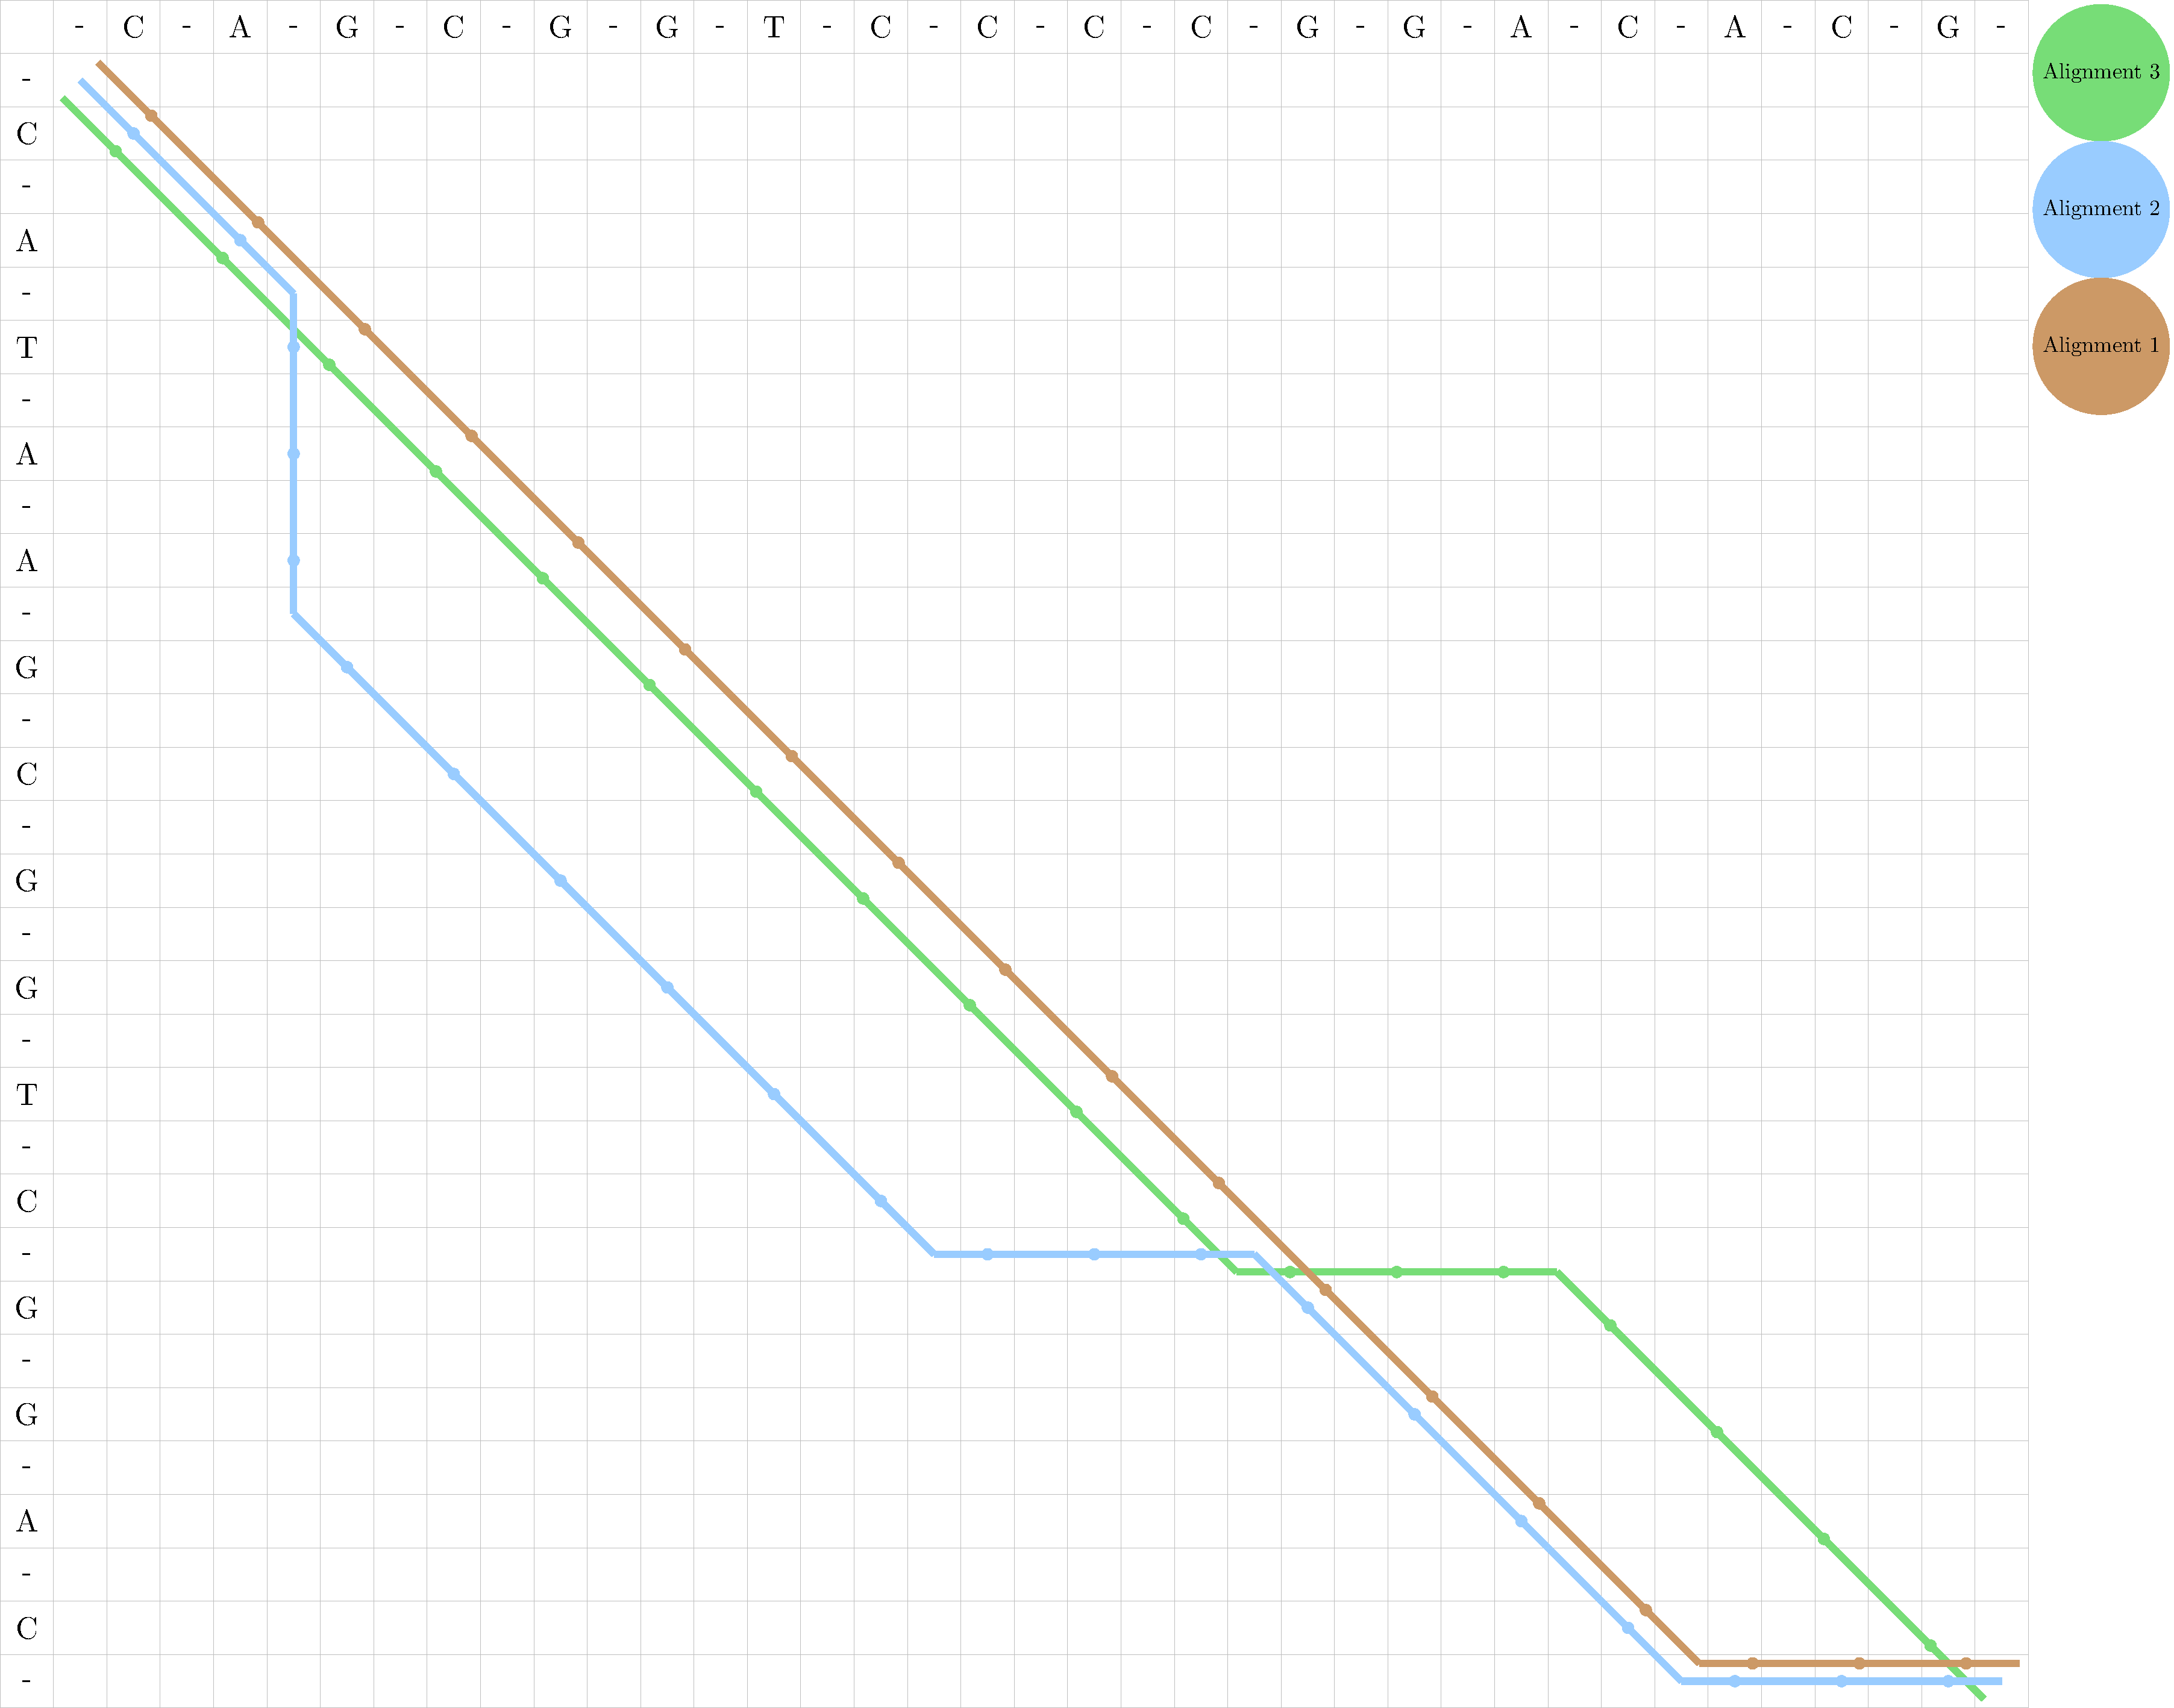
\includegraphics[width = 0.8\textwidth]{defense/figures/alndotplot/example-mlines.pdf}
% \end{columns}
% \end{frame} %-------------------------------------------------------------------

\begin{frame}[c]{Multiple Lines} %------------------------------------------------
\begin{columns}
    \column{0.3\textwidth}
        Small differences with long sequences are difficult to identify (180 nucs).
    \column{0.7\textwidth}
        \centering
        % \scalebox{0.02}{% Created by tikzDevice version 0.12.5 on 2023-10-08 23:51:01
% !TEX encoding = UTF-8 Unicode
\definecolor{color1}{HTML}{CC9966}
\definecolor{color2}{HTML}{99CCFF}
\begin{tikzpicture}[dot/.style={circle, minimum size=5mm}]
\draw[very thin, color = gray!15, step = 1] (0,0) grid (356, 338);
\node [scale=2] at (0.5,336.5) {-};
\node [scale=2] at (0.5,335.5) {C};
\node [scale=2] at (0.5,334.5) {-};
\node [scale=2] at (0.5,333.5) {C};
\node [scale=2] at (0.5,332.5) {-};
\node [scale=2] at (0.5,331.5) {G};
\node [scale=2] at (0.5,330.5) {-};
\node [scale=2] at (0.5,329.5) {A};
\node [scale=2] at (0.5,328.5) {-};
\node [scale=2] at (0.5,327.5) {A};
\node [scale=2] at (0.5,326.5) {-};
\node [scale=2] at (0.5,325.5) {C};
\node [scale=2] at (0.5,324.5) {-};
\node [scale=2] at (0.5,323.5) {G};
\node [scale=2] at (0.5,322.5) {-};
\node [scale=2] at (0.5,321.5) {A};
\node [scale=2] at (0.5,320.5) {-};
\node [scale=2] at (0.5,319.5) {C};
\node [scale=2] at (0.5,318.5) {-};
\node [scale=2] at (0.5,317.5) {G};
\node [scale=2] at (0.5,316.5) {-};
\node [scale=2] at (0.5,315.5) {G};
\node [scale=2] at (0.5,314.5) {-};
\node [scale=2] at (0.5,313.5) {G};
\node [scale=2] at (0.5,312.5) {-};
\node [scale=2] at (0.5,311.5) {C};
\node [scale=2] at (0.5,310.5) {-};
\node [scale=2] at (0.5,309.5) {G};
\node [scale=2] at (0.5,308.5) {-};
\node [scale=2] at (0.5,307.5) {C};
\node [scale=2] at (0.5,306.5) {-};
\node [scale=2] at (0.5,305.5) {T};
\node [scale=2] at (0.5,304.5) {-};
\node [scale=2] at (0.5,303.5) {G};
\node [scale=2] at (0.5,302.5) {-};
\node [scale=2] at (0.5,301.5) {T};
\node [scale=2] at (0.5,300.5) {-};
\node [scale=2] at (0.5,299.5) {C};
\node [scale=2] at (0.5,298.5) {-};
\node [scale=2] at (0.5,297.5) {A};
\node [scale=2] at (0.5,296.5) {-};
\node [scale=2] at (0.5,295.5) {T};
\node [scale=2] at (0.5,294.5) {-};
\node [scale=2] at (0.5,293.5) {A};
\node [scale=2] at (0.5,292.5) {-};
\node [scale=2] at (0.5,291.5) {T};
\node [scale=2] at (0.5,290.5) {-};
\node [scale=2] at (0.5,289.5) {G};
\node [scale=2] at (0.5,288.5) {-};
\node [scale=2] at (0.5,287.5) {G};
\node [scale=2] at (0.5,286.5) {-};
\node [scale=2] at (0.5,285.5) {A};
\node [scale=2] at (0.5,284.5) {-};
\node [scale=2] at (0.5,283.5) {G};
\node [scale=2] at (0.5,282.5) {-};
\node [scale=2] at (0.5,281.5) {G};
\node [scale=2] at (0.5,280.5) {-};
\node [scale=2] at (0.5,279.5) {A};
\node [scale=2] at (0.5,278.5) {-};
\node [scale=2] at (0.5,277.5) {T};
\node [scale=2] at (0.5,276.5) {-};
\node [scale=2] at (0.5,275.5) {G};
\node [scale=2] at (0.5,274.5) {-};
\node [scale=2] at (0.5,273.5) {A};
\node [scale=2] at (0.5,272.5) {-};
\node [scale=2] at (0.5,271.5) {C};
\node [scale=2] at (0.5,270.5) {-};
\node [scale=2] at (0.5,269.5) {T};
\node [scale=2] at (0.5,268.5) {-};
\node [scale=2] at (0.5,267.5) {T};
\node [scale=2] at (0.5,266.5) {-};
\node [scale=2] at (0.5,265.5) {G};
\node [scale=2] at (0.5,264.5) {-};
\node [scale=2] at (0.5,263.5) {T};
\node [scale=2] at (0.5,262.5) {-};
\node [scale=2] at (0.5,261.5) {A};
\node [scale=2] at (0.5,260.5) {-};
\node [scale=2] at (0.5,259.5) {C};
\node [scale=2] at (0.5,258.5) {-};
\node [scale=2] at (0.5,257.5) {A};
\node [scale=2] at (0.5,256.5) {-};
\node [scale=2] at (0.5,255.5) {A};
\node [scale=2] at (0.5,254.5) {-};
\node [scale=2] at (0.5,253.5) {G};
\node [scale=2] at (0.5,252.5) {-};
\node [scale=2] at (0.5,251.5) {A};
\node [scale=2] at (0.5,250.5) {-};
\node [scale=2] at (0.5,249.5) {G};
\node [scale=2] at (0.5,248.5) {-};
\node [scale=2] at (0.5,247.5) {G};
\node [scale=2] at (0.5,246.5) {-};
\node [scale=2] at (0.5,245.5) {A};
\node [scale=2] at (0.5,244.5) {-};
\node [scale=2] at (0.5,243.5) {G};
\node [scale=2] at (0.5,242.5) {-};
\node [scale=2] at (0.5,241.5) {C};
\node [scale=2] at (0.5,240.5) {-};
\node [scale=2] at (0.5,239.5) {A};
\node [scale=2] at (0.5,238.5) {-};
\node [scale=2] at (0.5,237.5) {C};
\node [scale=2] at (0.5,236.5) {-};
\node [scale=2] at (0.5,235.5) {A};
\node [scale=2] at (0.5,234.5) {-};
\node [scale=2] at (0.5,233.5) {C};
\node [scale=2] at (0.5,232.5) {-};
\node [scale=2] at (0.5,231.5) {T};
\node [scale=2] at (0.5,230.5) {-};
\node [scale=2] at (0.5,229.5) {G};
\node [scale=2] at (0.5,228.5) {-};
\node [scale=2] at (0.5,227.5) {A};
\node [scale=2] at (0.5,226.5) {-};
\node [scale=2] at (0.5,225.5) {A};
\node [scale=2] at (0.5,224.5) {-};
\node [scale=2] at (0.5,223.5) {A};
\node [scale=2] at (0.5,222.5) {-};
\node [scale=2] at (0.5,221.5) {G};
\node [scale=2] at (0.5,220.5) {-};
\node [scale=2] at (0.5,219.5) {T};
\node [scale=2] at (0.5,218.5) {-};
\node [scale=2] at (0.5,217.5) {C};
\node [scale=2] at (0.5,216.5) {-};
\node [scale=2] at (0.5,215.5) {A};
\node [scale=2] at (0.5,214.5) {-};
\node [scale=2] at (0.5,213.5) {C};
\node [scale=2] at (0.5,212.5) {-};
\node [scale=2] at (0.5,211.5) {C};
\node [scale=2] at (0.5,210.5) {-};
\node [scale=2] at (0.5,209.5) {T};
\node [scale=2] at (0.5,208.5) {-};
\node [scale=2] at (0.5,207.5) {A};
\node [scale=2] at (0.5,206.5) {-};
\node [scale=2] at (0.5,205.5) {C};
\node [scale=2] at (0.5,204.5) {-};
\node [scale=2] at (0.5,203.5) {G};
\node [scale=2] at (0.5,202.5) {-};
\node [scale=2] at (0.5,201.5) {T};
\node [scale=2] at (0.5,200.5) {-};
\node [scale=2] at (0.5,199.5) {C};
\node [scale=2] at (0.5,198.5) {-};
\node [scale=2] at (0.5,197.5) {T};
\node [scale=2] at (0.5,196.5) {-};
\node [scale=2] at (0.5,195.5) {C};
\node [scale=2] at (0.5,194.5) {-};
\node [scale=2] at (0.5,193.5) {C};
\node [scale=2] at (0.5,192.5) {-};
\node [scale=2] at (0.5,191.5) {T};
\node [scale=2] at (0.5,190.5) {-};
\node [scale=2] at (0.5,189.5) {A};
\node [scale=2] at (0.5,188.5) {-};
\node [scale=2] at (0.5,187.5) {T};
\node [scale=2] at (0.5,186.5) {-};
\node [scale=2] at (0.5,185.5) {T};
\node [scale=2] at (0.5,184.5) {-};
\node [scale=2] at (0.5,183.5) {A};
\node [scale=2] at (0.5,182.5) {-};
\node [scale=2] at (0.5,181.5) {C};
\node [scale=2] at (0.5,180.5) {-};
\node [scale=2] at (0.5,179.5) {A};
\node [scale=2] at (0.5,178.5) {-};
\node [scale=2] at (0.5,177.5) {A};
\node [scale=2] at (0.5,176.5) {-};
\node [scale=2] at (0.5,175.5) {C};
\node [scale=2] at (0.5,174.5) {-};
\node [scale=2] at (0.5,173.5) {A};
\node [scale=2] at (0.5,172.5) {-};
\node [scale=2] at (0.5,171.5) {A};
\node [scale=2] at (0.5,170.5) {-};
\node [scale=2] at (0.5,169.5) {T};
\node [scale=2] at (0.5,168.5) {-};
\node [scale=2] at (0.5,167.5) {G};
\node [scale=2] at (0.5,166.5) {-};
\node [scale=2] at (0.5,165.5) {G};
\node [scale=2] at (0.5,164.5) {-};
\node [scale=2] at (0.5,163.5) {A};
\node [scale=2] at (0.5,162.5) {-};
\node [scale=2] at (0.5,161.5) {G};
\node [scale=2] at (0.5,160.5) {-};
\node [scale=2] at (0.5,159.5) {T};
\node [scale=2] at (0.5,158.5) {-};
\node [scale=2] at (0.5,157.5) {G};
\node [scale=2] at (0.5,156.5) {-};
\node [scale=2] at (0.5,155.5) {A};
\node [scale=2] at (0.5,154.5) {-};
\node [scale=2] at (0.5,153.5) {C};
\node [scale=2] at (0.5,152.5) {-};
\node [scale=2] at (0.5,151.5) {G};
\node [scale=2] at (0.5,150.5) {-};
\node [scale=2] at (0.5,149.5) {C};
\node [scale=2] at (0.5,148.5) {-};
\node [scale=2] at (0.5,147.5) {A};
\node [scale=2] at (0.5,146.5) {-};
\node [scale=2] at (0.5,145.5) {C};
\node [scale=2] at (0.5,144.5) {-};
\node [scale=2] at (0.5,143.5) {A};
\node [scale=2] at (0.5,142.5) {-};
\node [scale=2] at (0.5,141.5) {G};
\node [scale=2] at (0.5,140.5) {-};
\node [scale=2] at (0.5,139.5) {G};
\node [scale=2] at (0.5,138.5) {-};
\node [scale=2] at (0.5,137.5) {A};
\node [scale=2] at (0.5,136.5) {-};
\node [scale=2] at (0.5,135.5) {A};
\node [scale=2] at (0.5,134.5) {-};
\node [scale=2] at (0.5,133.5) {T};
\node [scale=2] at (0.5,132.5) {-};
\node [scale=2] at (0.5,131.5) {C};
\node [scale=2] at (0.5,130.5) {-};
\node [scale=2] at (0.5,129.5) {A};
\node [scale=2] at (0.5,128.5) {-};
\node [scale=2] at (0.5,127.5) {G};
\node [scale=2] at (0.5,126.5) {-};
\node [scale=2] at (0.5,125.5) {C};
\node [scale=2] at (0.5,124.5) {-};
\node [scale=2] at (0.5,123.5) {C};
\node [scale=2] at (0.5,122.5) {-};
\node [scale=2] at (0.5,121.5) {C};
\node [scale=2] at (0.5,120.5) {-};
\node [scale=2] at (0.5,119.5) {A};
\node [scale=2] at (0.5,118.5) {-};
\node [scale=2] at (0.5,117.5) {G};
\node [scale=2] at (0.5,116.5) {-};
\node [scale=2] at (0.5,115.5) {A};
\node [scale=2] at (0.5,114.5) {-};
\node [scale=2] at (0.5,113.5) {G};
\node [scale=2] at (0.5,112.5) {-};
\node [scale=2] at (0.5,111.5) {G};
\node [scale=2] at (0.5,110.5) {-};
\node [scale=2] at (0.5,109.5) {T};
\node [scale=2] at (0.5,108.5) {-};
\node [scale=2] at (0.5,107.5) {G};
\node [scale=2] at (0.5,106.5) {-};
\node [scale=2] at (0.5,105.5) {A};
\node [scale=2] at (0.5,104.5) {-};
\node [scale=2] at (0.5,103.5) {C};
\node [scale=2] at (0.5,102.5) {-};
\node [scale=2] at (0.5,101.5) {T};
\node [scale=2] at (0.5,100.5) {-};
\node [scale=2] at (0.5,99.5) {G};
\node [scale=2] at (0.5,98.5) {-};
\node [scale=2] at (0.5,97.5) {T};
\node [scale=2] at (0.5,96.5) {-};
\node [scale=2] at (0.5,95.5) {G};
\node [scale=2] at (0.5,94.5) {-};
\node [scale=2] at (0.5,93.5) {A};
\node [scale=2] at (0.5,92.5) {-};
\node [scale=2] at (0.5,91.5) {T};
\node [scale=2] at (0.5,90.5) {-};
\node [scale=2] at (0.5,89.5) {G};
\node [scale=2] at (0.5,88.5) {-};
\node [scale=2] at (0.5,87.5) {G};
\node [scale=2] at (0.5,86.5) {-};
\node [scale=2] at (0.5,85.5) {C};
\node [scale=2] at (0.5,84.5) {-};
\node [scale=2] at (0.5,83.5) {G};
\node [scale=2] at (0.5,82.5) {-};
\node [scale=2] at (0.5,81.5) {C};
\node [scale=2] at (0.5,80.5) {-};
\node [scale=2] at (0.5,79.5) {G};
\node [scale=2] at (0.5,78.5) {-};
\node [scale=2] at (0.5,77.5) {C};
\node [scale=2] at (0.5,76.5) {-};
\node [scale=2] at (0.5,75.5) {A};
\node [scale=2] at (0.5,74.5) {-};
\node [scale=2] at (0.5,73.5) {A};
\node [scale=2] at (0.5,72.5) {-};
\node [scale=2] at (0.5,71.5) {A};
\node [scale=2] at (0.5,70.5) {-};
\node [scale=2] at (0.5,69.5) {T};
\node [scale=2] at (0.5,68.5) {-};
\node [scale=2] at (0.5,67.5) {C};
\node [scale=2] at (0.5,66.5) {-};
\node [scale=2] at (0.5,65.5) {A};
\node [scale=2] at (0.5,64.5) {-};
\node [scale=2] at (0.5,63.5) {A};
\node [scale=2] at (0.5,62.5) {-};
\node [scale=2] at (0.5,61.5) {C};
\node [scale=2] at (0.5,60.5) {-};
\node [scale=2] at (0.5,59.5) {G};
\node [scale=2] at (0.5,58.5) {-};
\node [scale=2] at (0.5,57.5) {T};
\node [scale=2] at (0.5,56.5) {-};
\node [scale=2] at (0.5,55.5) {C};
\node [scale=2] at (0.5,54.5) {-};
\node [scale=2] at (0.5,53.5) {C};
\node [scale=2] at (0.5,52.5) {-};
\node [scale=2] at (0.5,51.5) {C};
\node [scale=2] at (0.5,50.5) {-};
\node [scale=2] at (0.5,49.5) {A};
\node [scale=2] at (0.5,48.5) {-};
\node [scale=2] at (0.5,47.5) {A};
\node [scale=2] at (0.5,46.5) {-};
\node [scale=2] at (0.5,45.5) {T};
\node [scale=2] at (0.5,44.5) {-};
\node [scale=2] at (0.5,43.5) {C};
\node [scale=2] at (0.5,42.5) {-};
\node [scale=2] at (0.5,41.5) {A};
\node [scale=2] at (0.5,40.5) {-};
\node [scale=2] at (0.5,39.5) {C};
\node [scale=2] at (0.5,38.5) {-};
\node [scale=2] at (0.5,37.5) {C};
\node [scale=2] at (0.5,36.5) {-};
\node [scale=2] at (0.5,35.5) {T};
\node [scale=2] at (0.5,34.5) {-};
\node [scale=2] at (0.5,33.5) {T};
\node [scale=2] at (0.5,32.5) {-};
\node [scale=2] at (0.5,31.5) {C};
\node [scale=2] at (0.5,30.5) {-};
\node [scale=2] at (0.5,29.5) {A};
\node [scale=2] at (0.5,28.5) {-};
\node [scale=2] at (0.5,27.5) {A};
\node [scale=2] at (0.5,26.5) {-};
\node [scale=2] at (0.5,25.5) {G};
\node [scale=2] at (0.5,24.5) {-};
\node [scale=2] at (0.5,23.5) {G};
\node [scale=2] at (0.5,22.5) {-};
\node [scale=2] at (0.5,21.5) {T};
\node [scale=2] at (0.5,20.5) {-};
\node [scale=2] at (0.5,19.5) {G};
\node [scale=2] at (0.5,18.5) {-};
\node [scale=2] at (0.5,17.5) {G};
\node [scale=2] at (0.5,16.5) {-};
\node [scale=2] at (0.5,15.5) {G};
\node [scale=2] at (0.5,14.5) {-};
\node [scale=2] at (0.5,13.5) {G};
\node [scale=2] at (0.5,12.5) {-};
\node [scale=2] at (0.5,11.5) {G};
\node [scale=2] at (0.5,10.5) {-};
\node [scale=2] at (0.5,9.5) {T};
\node [scale=2] at (0.5,8.5) {-};
\node [scale=2] at (0.5,7.5) {C};
\node [scale=2] at (0.5,6.5) {-};
\node [scale=2] at (0.5,5.5) {A};
\node [scale=2] at (0.5,4.5) {-};
\node [scale=2] at (0.5,3.5) {C};
\node [scale=2] at (0.5,2.5) {-};
\node [scale=2] at (0.5,1.5) {G};
\node [scale=2] at (0.5,0.5) {-};
\node [scale=2] at (1.5,337.5) {-};
\node [scale=2] at (2.5,337.5) {A};
\node [scale=2] at (3.5,337.5) {-};
\node [scale=2] at (4.5,337.5) {C};
\node [scale=2] at (5.5,337.5) {-};
\node [scale=2] at (6.5,337.5) {C};
\node [scale=2] at (7.5,337.5) {-};
\node [scale=2] at (8.5,337.5) {A};
\node [scale=2] at (9.5,337.5) {-};
\node [scale=2] at (10.5,337.5) {A};
\node [scale=2] at (11.5,337.5) {-};
\node [scale=2] at (12.5,337.5) {C};
\node [scale=2] at (13.5,337.5) {-};
\node [scale=2] at (14.5,337.5) {G};
\node [scale=2] at (15.5,337.5) {-};
\node [scale=2] at (16.5,337.5) {A};
\node [scale=2] at (17.5,337.5) {-};
\node [scale=2] at (18.5,337.5) {A};
\node [scale=2] at (19.5,337.5) {-};
\node [scale=2] at (20.5,337.5) {G};
\node [scale=2] at (21.5,337.5) {-};
\node [scale=2] at (22.5,337.5) {G};
\node [scale=2] at (23.5,337.5) {-};
\node [scale=2] at (24.5,337.5) {G};
\node [scale=2] at (25.5,337.5) {-};
\node [scale=2] at (26.5,337.5) {C};
\node [scale=2] at (27.5,337.5) {-};
\node [scale=2] at (28.5,337.5) {A};
\node [scale=2] at (29.5,337.5) {-};
\node [scale=2] at (30.5,337.5) {T};
\node [scale=2] at (31.5,337.5) {-};
\node [scale=2] at (32.5,337.5) {T};
\node [scale=2] at (33.5,337.5) {-};
\node [scale=2] at (34.5,337.5) {G};
\node [scale=2] at (35.5,337.5) {-};
\node [scale=2] at (36.5,337.5) {T};
\node [scale=2] at (37.5,337.5) {-};
\node [scale=2] at (38.5,337.5) {C};
\node [scale=2] at (39.5,337.5) {-};
\node [scale=2] at (40.5,337.5) {A};
\node [scale=2] at (41.5,337.5) {-};
\node [scale=2] at (42.5,337.5) {C};
\node [scale=2] at (43.5,337.5) {-};
\node [scale=2] at (44.5,337.5) {C};
\node [scale=2] at (45.5,337.5) {-};
\node [scale=2] at (46.5,337.5) {T};
\node [scale=2] at (47.5,337.5) {-};
\node [scale=2] at (48.5,337.5) {G};
\node [scale=2] at (49.5,337.5) {-};
\node [scale=2] at (50.5,337.5) {G};
\node [scale=2] at (51.5,337.5) {-};
\node [scale=2] at (52.5,337.5) {A};
\node [scale=2] at (53.5,337.5) {-};
\node [scale=2] at (54.5,337.5) {G};
\node [scale=2] at (55.5,337.5) {-};
\node [scale=2] at (56.5,337.5) {G};
\node [scale=2] at (57.5,337.5) {-};
\node [scale=2] at (58.5,337.5) {A};
\node [scale=2] at (59.5,337.5) {-};
\node [scale=2] at (60.5,337.5) {C};
\node [scale=2] at (61.5,337.5) {-};
\node [scale=2] at (62.5,337.5) {A};
\node [scale=2] at (63.5,337.5) {-};
\node [scale=2] at (64.5,337.5) {A};
\node [scale=2] at (65.5,337.5) {-};
\node [scale=2] at (66.5,337.5) {T};
\node [scale=2] at (67.5,337.5) {-};
\node [scale=2] at (68.5,337.5) {T};
\node [scale=2] at (69.5,337.5) {-};
\node [scale=2] at (70.5,337.5) {T};
\node [scale=2] at (71.5,337.5) {-};
\node [scale=2] at (72.5,337.5) {T};
\node [scale=2] at (73.5,337.5) {-};
\node [scale=2] at (74.5,337.5) {T};
\node [scale=2] at (75.5,337.5) {-};
\node [scale=2] at (76.5,337.5) {A};
\node [scale=2] at (77.5,337.5) {-};
\node [scale=2] at (78.5,337.5) {C};
\node [scale=2] at (79.5,337.5) {-};
\node [scale=2] at (80.5,337.5) {A};
\node [scale=2] at (81.5,337.5) {-};
\node [scale=2] at (82.5,337.5) {A};
\node [scale=2] at (83.5,337.5) {-};
\node [scale=2] at (84.5,337.5) {T};
\node [scale=2] at (85.5,337.5) {-};
\node [scale=2] at (86.5,337.5) {A};
\node [scale=2] at (87.5,337.5) {-};
\node [scale=2] at (88.5,337.5) {A};
\node [scale=2] at (89.5,337.5) {-};
\node [scale=2] at (90.5,337.5) {T};
\node [scale=2] at (91.5,337.5) {-};
\node [scale=2] at (92.5,337.5) {A};
\node [scale=2] at (93.5,337.5) {-};
\node [scale=2] at (94.5,337.5) {T};
\node [scale=2] at (95.5,337.5) {-};
\node [scale=2] at (96.5,337.5) {T};
\node [scale=2] at (97.5,337.5) {-};
\node [scale=2] at (98.5,337.5) {T};
\node [scale=2] at (99.5,337.5) {-};
\node [scale=2] at (100.5,337.5) {A};
\node [scale=2] at (101.5,337.5) {-};
\node [scale=2] at (102.5,337.5) {C};
\node [scale=2] at (103.5,337.5) {-};
\node [scale=2] at (104.5,337.5) {A};
\node [scale=2] at (105.5,337.5) {-};
\node [scale=2] at (106.5,337.5) {A};
\node [scale=2] at (107.5,337.5) {-};
\node [scale=2] at (108.5,337.5) {A};
\node [scale=2] at (109.5,337.5) {-};
\node [scale=2] at (110.5,337.5) {A};
\node [scale=2] at (111.5,337.5) {-};
\node [scale=2] at (112.5,337.5) {G};
\node [scale=2] at (113.5,337.5) {-};
\node [scale=2] at (114.5,337.5) {G};
\node [scale=2] at (115.5,337.5) {-};
\node [scale=2] at (116.5,337.5) {A};
\node [scale=2] at (117.5,337.5) {-};
\node [scale=2] at (118.5,337.5) {G};
\node [scale=2] at (119.5,337.5) {-};
\node [scale=2] at (120.5,337.5) {T};
\node [scale=2] at (121.5,337.5) {-};
\node [scale=2] at (122.5,337.5) {A};
\node [scale=2] at (123.5,337.5) {-};
\node [scale=2] at (124.5,337.5) {T};
\node [scale=2] at (125.5,337.5) {-};
\node [scale=2] at (126.5,337.5) {C};
\node [scale=2] at (127.5,337.5) {-};
\node [scale=2] at (128.5,337.5) {C};
\node [scale=2] at (129.5,337.5) {-};
\node [scale=2] at (130.5,337.5) {T};
\node [scale=2] at (131.5,337.5) {-};
\node [scale=2] at (132.5,337.5) {A};
\node [scale=2] at (133.5,337.5) {-};
\node [scale=2] at (134.5,337.5) {A};
\node [scale=2] at (135.5,337.5) {-};
\node [scale=2] at (136.5,337.5) {A};
\node [scale=2] at (137.5,337.5) {-};
\node [scale=2] at (138.5,337.5) {A};
\node [scale=2] at (139.5,337.5) {-};
\node [scale=2] at (140.5,337.5) {G};
\node [scale=2] at (141.5,337.5) {-};
\node [scale=2] at (142.5,337.5) {T};
\node [scale=2] at (143.5,337.5) {-};
\node [scale=2] at (144.5,337.5) {A};
\node [scale=2] at (145.5,337.5) {-};
\node [scale=2] at (146.5,337.5) {A};
\node [scale=2] at (147.5,337.5) {-};
\node [scale=2] at (148.5,337.5) {C};
\node [scale=2] at (149.5,337.5) {-};
\node [scale=2] at (150.5,337.5) {A};
\node [scale=2] at (151.5,337.5) {-};
\node [scale=2] at (152.5,337.5) {T};
\node [scale=2] at (153.5,337.5) {-};
\node [scale=2] at (154.5,337.5) {A};
\node [scale=2] at (155.5,337.5) {-};
\node [scale=2] at (156.5,337.5) {C};
\node [scale=2] at (157.5,337.5) {-};
\node [scale=2] at (158.5,337.5) {A};
\node [scale=2] at (159.5,337.5) {-};
\node [scale=2] at (160.5,337.5) {G};
\node [scale=2] at (161.5,337.5) {-};
\node [scale=2] at (162.5,337.5) {T};
\node [scale=2] at (163.5,337.5) {-};
\node [scale=2] at (164.5,337.5) {T};
\node [scale=2] at (165.5,337.5) {-};
\node [scale=2] at (166.5,337.5) {C};
\node [scale=2] at (167.5,337.5) {-};
\node [scale=2] at (168.5,337.5) {A};
\node [scale=2] at (169.5,337.5) {-};
\node [scale=2] at (170.5,337.5) {T};
\node [scale=2] at (171.5,337.5) {-};
\node [scale=2] at (172.5,337.5) {T};
\node [scale=2] at (173.5,337.5) {-};
\node [scale=2] at (174.5,337.5) {C};
\node [scale=2] at (175.5,337.5) {-};
\node [scale=2] at (176.5,337.5) {T};
\node [scale=2] at (177.5,337.5) {-};
\node [scale=2] at (178.5,337.5) {G};
\node [scale=2] at (179.5,337.5) {-};
\node [scale=2] at (180.5,337.5) {C};
\node [scale=2] at (181.5,337.5) {-};
\node [scale=2] at (182.5,337.5) {A};
\node [scale=2] at (183.5,337.5) {-};
\node [scale=2] at (184.5,337.5) {G};
\node [scale=2] at (185.5,337.5) {-};
\node [scale=2] at (186.5,337.5) {T};
\node [scale=2] at (187.5,337.5) {-};
\node [scale=2] at (188.5,337.5) {A};
\node [scale=2] at (189.5,337.5) {-};
\node [scale=2] at (190.5,337.5) {G};
\node [scale=2] at (191.5,337.5) {-};
\node [scale=2] at (192.5,337.5) {T};
\node [scale=2] at (193.5,337.5) {-};
\node [scale=2] at (194.5,337.5) {A};
\node [scale=2] at (195.5,337.5) {-};
\node [scale=2] at (196.5,337.5) {G};
\node [scale=2] at (197.5,337.5) {-};
\node [scale=2] at (198.5,337.5) {A};
\node [scale=2] at (199.5,337.5) {-};
\node [scale=2] at (200.5,337.5) {G};
\node [scale=2] at (201.5,337.5) {-};
\node [scale=2] at (202.5,337.5) {T};
\node [scale=2] at (203.5,337.5) {-};
\node [scale=2] at (204.5,337.5) {G};
\node [scale=2] at (205.5,337.5) {-};
\node [scale=2] at (206.5,337.5) {A};
\node [scale=2] at (207.5,337.5) {-};
\node [scale=2] at (208.5,337.5) {C};
\node [scale=2] at (209.5,337.5) {-};
\node [scale=2] at (210.5,337.5) {G};
\node [scale=2] at (211.5,337.5) {-};
\node [scale=2] at (212.5,337.5) {C};
\node [scale=2] at (213.5,337.5) {-};
\node [scale=2] at (214.5,337.5) {A};
\node [scale=2] at (215.5,337.5) {-};
\node [scale=2] at (216.5,337.5) {C};
\node [scale=2] at (217.5,337.5) {-};
\node [scale=2] at (218.5,337.5) {A};
\node [scale=2] at (219.5,337.5) {-};
\node [scale=2] at (220.5,337.5) {G};
\node [scale=2] at (221.5,337.5) {-};
\node [scale=2] at (222.5,337.5) {G};
\node [scale=2] at (223.5,337.5) {-};
\node [scale=2] at (224.5,337.5) {A};
\node [scale=2] at (225.5,337.5) {-};
\node [scale=2] at (226.5,337.5) {A};
\node [scale=2] at (227.5,337.5) {-};
\node [scale=2] at (228.5,337.5) {T};
\node [scale=2] at (229.5,337.5) {-};
\node [scale=2] at (230.5,337.5) {C};
\node [scale=2] at (231.5,337.5) {-};
\node [scale=2] at (232.5,337.5) {G};
\node [scale=2] at (233.5,337.5) {-};
\node [scale=2] at (234.5,337.5) {G};
\node [scale=2] at (235.5,337.5) {-};
\node [scale=2] at (236.5,337.5) {C};
\node [scale=2] at (237.5,337.5) {-};
\node [scale=2] at (238.5,337.5) {T};
\node [scale=2] at (239.5,337.5) {-};
\node [scale=2] at (240.5,337.5) {A};
\node [scale=2] at (241.5,337.5) {-};
\node [scale=2] at (242.5,337.5) {G};
\node [scale=2] at (243.5,337.5) {-};
\node [scale=2] at (244.5,337.5) {G};
\node [scale=2] at (245.5,337.5) {-};
\node [scale=2] at (246.5,337.5) {T};
\node [scale=2] at (247.5,337.5) {-};
\node [scale=2] at (248.5,337.5) {G};
\node [scale=2] at (249.5,337.5) {-};
\node [scale=2] at (250.5,337.5) {A};
\node [scale=2] at (251.5,337.5) {-};
\node [scale=2] at (252.5,337.5) {T};
\node [scale=2] at (253.5,337.5) {-};
\node [scale=2] at (254.5,337.5) {T};
\node [scale=2] at (255.5,337.5) {-};
\node [scale=2] at (256.5,337.5) {G};
\node [scale=2] at (257.5,337.5) {-};
\node [scale=2] at (258.5,337.5) {G};
\node [scale=2] at (259.5,337.5) {-};
\node [scale=2] at (260.5,337.5) {T};
\node [scale=2] at (261.5,337.5) {-};
\node [scale=2] at (262.5,337.5) {A};
\node [scale=2] at (263.5,337.5) {-};
\node [scale=2] at (264.5,337.5) {T};
\node [scale=2] at (265.5,337.5) {-};
\node [scale=2] at (266.5,337.5) {G};
\node [scale=2] at (267.5,337.5) {-};
\node [scale=2] at (268.5,337.5) {G};
\node [scale=2] at (269.5,337.5) {-};
\node [scale=2] at (270.5,337.5) {T};
\node [scale=2] at (271.5,337.5) {-};
\node [scale=2] at (272.5,337.5) {G};
\node [scale=2] at (273.5,337.5) {-};
\node [scale=2] at (274.5,337.5) {T};
\node [scale=2] at (275.5,337.5) {-};
\node [scale=2] at (276.5,337.5) {G};
\node [scale=2] at (277.5,337.5) {-};
\node [scale=2] at (278.5,337.5) {C};
\node [scale=2] at (279.5,337.5) {-};
\node [scale=2] at (280.5,337.5) {A};
\node [scale=2] at (281.5,337.5) {-};
\node [scale=2] at (282.5,337.5) {G};
\node [scale=2] at (283.5,337.5) {-};
\node [scale=2] at (284.5,337.5) {A};
\node [scale=2] at (285.5,337.5) {-};
\node [scale=2] at (286.5,337.5) {A};
\node [scale=2] at (287.5,337.5) {-};
\node [scale=2] at (288.5,337.5) {T};
\node [scale=2] at (289.5,337.5) {-};
\node [scale=2] at (290.5,337.5) {A};
\node [scale=2] at (291.5,337.5) {-};
\node [scale=2] at (292.5,337.5) {A};
\node [scale=2] at (293.5,337.5) {-};
\node [scale=2] at (294.5,337.5) {T};
\node [scale=2] at (295.5,337.5) {-};
\node [scale=2] at (296.5,337.5) {G};
\node [scale=2] at (297.5,337.5) {-};
\node [scale=2] at (298.5,337.5) {T};
\node [scale=2] at (299.5,337.5) {-};
\node [scale=2] at (300.5,337.5) {T};
\node [scale=2] at (301.5,337.5) {-};
\node [scale=2] at (302.5,337.5) {C};
\node [scale=2] at (303.5,337.5) {-};
\node [scale=2] at (304.5,337.5) {C};
\node [scale=2] at (305.5,337.5) {-};
\node [scale=2] at (306.5,337.5) {G};
\node [scale=2] at (307.5,337.5) {-};
\node [scale=2] at (308.5,337.5) {A};
\node [scale=2] at (309.5,337.5) {-};
\node [scale=2] at (310.5,337.5) {T};
\node [scale=2] at (311.5,337.5) {-};
\node [scale=2] at (312.5,337.5) {C};
\node [scale=2] at (313.5,337.5) {-};
\node [scale=2] at (314.5,337.5) {A};
\node [scale=2] at (315.5,337.5) {-};
\node [scale=2] at (316.5,337.5) {C};
\node [scale=2] at (317.5,337.5) {-};
\node [scale=2] at (318.5,337.5) {C};
\node [scale=2] at (319.5,337.5) {-};
\node [scale=2] at (320.5,337.5) {T};
\node [scale=2] at (321.5,337.5) {-};
\node [scale=2] at (322.5,337.5) {T};
\node [scale=2] at (323.5,337.5) {-};
\node [scale=2] at (324.5,337.5) {C};
\node [scale=2] at (325.5,337.5) {-};
\node [scale=2] at (326.5,337.5) {C};
\node [scale=2] at (327.5,337.5) {-};
\node [scale=2] at (328.5,337.5) {A};
\node [scale=2] at (329.5,337.5) {-};
\node [scale=2] at (330.5,337.5) {A};
\node [scale=2] at (331.5,337.5) {-};
\node [scale=2] at (332.5,337.5) {A};
\node [scale=2] at (333.5,337.5) {-};
\node [scale=2] at (334.5,337.5) {T};
\node [scale=2] at (335.5,337.5) {-};
\node [scale=2] at (336.5,337.5) {G};
\node [scale=2] at (337.5,337.5) {-};
\node [scale=2] at (338.5,337.5) {A};
\node [scale=2] at (339.5,337.5) {-};
\node [scale=2] at (340.5,337.5) {A};
\node [scale=2] at (341.5,337.5) {-};
\node [scale=2] at (342.5,337.5) {G};
\node [scale=2] at (343.5,337.5) {-};
\node [scale=2] at (344.5,337.5) {G};
\node [scale=2] at (345.5,337.5) {-};
\node [scale=2] at (346.5,337.5) {T};
\node [scale=2] at (347.5,337.5) {-};
\node [scale=2] at (348.5,337.5) {C};
\node [scale=2] at (349.5,337.5) {-};
\node [scale=2] at (350.5,337.5) {A};
\node [scale=2] at (351.5,337.5) {-};
\node [scale=2] at (352.5,337.5) {C};
\node [scale=2] at (353.5,337.5) {-};
\node [scale=2] at (354.5,337.5) {G};
\node [scale=2] at (355.5,337.5) {-};
\draw[line width=1.25mm,color1](1.25,336.25)--(2.25,335.25);
\node[circle, fill=color1] at (1.25, 336.25){};
\draw[line width=1.25mm,color1](2.25,335.25)--(3.25,334.25);
\node[circle, fill=color1] at (2.25, 335.25){};
\draw[line width=1.25mm,color1](3.25,334.25)--(4.25,333.25);
\node[circle, fill=color1] at (3.25, 334.25){};
\draw[line width=1.25mm,color1](4.25,333.25)--(5.25,332.25);
\node[circle, fill=color1] at (4.25, 333.25){};
\draw[line width=1.25mm,color1](5.25,332.25)--(6.25,331.25);
\node[circle, fill=color1] at (5.25, 332.25){};
\draw[line width=1.25mm,color1](6.25,331.25)--(7.25,330.25);
\node[circle, fill=color1] at (6.25, 331.25){};
\draw[line width=1.25mm,color1](7.25,330.25)--(8.25,329.25);
\node[circle, fill=color1] at (7.25, 330.25){};
\draw[line width=1.25mm,color1](8.25,329.25)--(9.25,328.25);
\node[circle, fill=color1] at (8.25, 329.25){};
\draw[line width=1.25mm,color1](9.25,328.25)--(10.25,327.25);
\node[circle, fill=color1] at (9.25, 328.25){};
\draw[line width=1.25mm,color1](10.25,327.25)--(11.25,326.25);
\node[circle, fill=color1] at (10.25, 327.25){};
\draw[line width=1.25mm,color1](11.25,326.25)--(12.25,325.25);
\node[circle, fill=color1] at (11.25, 326.25){};
\draw[line width=1.25mm,color1](12.25,325.25)--(13.25,324.25);
\node[circle, fill=color1] at (12.25, 325.25){};
\draw[line width=1.25mm,color1](13.25,324.25)--(14.25,323.25);
\node[circle, fill=color1] at (13.25, 324.25){};
\draw[line width=1.25mm,color1](14.25,323.25)--(15.25,322.25);
\node[circle, fill=color1] at (14.25, 323.25){};
\draw[line width=1.25mm,color1](15.25,322.25)--(16.25,321.25);
\node[circle, fill=color1] at (15.25, 322.25){};
\draw[line width=1.25mm,color1](16.25,321.25)--(17.25,320.25);
\node[circle, fill=color1] at (16.25, 321.25){};
\draw[line width=1.25mm,color1](17.25,320.25)--(18.25,319.25);
\node[circle, fill=color1] at (17.25, 320.25){};
\draw[line width=1.25mm,color1](18.25,319.25)--(19.25,318.25);
\node[circle, fill=color1] at (18.25, 319.25){};
\draw[line width=1.25mm,color1](19.25,318.25)--(20.25,317.25);
\node[circle, fill=color1] at (19.25, 318.25){};
\draw[line width=1.25mm,color1](20.25,317.25)--(21.25,316.25);
\node[circle, fill=color1] at (20.25, 317.25){};
\draw[line width=1.25mm,color1](21.25,316.25)--(22.25,315.25);
\node[circle, fill=color1] at (21.25, 316.25){};
\draw[line width=1.25mm,color1](22.25,315.25)--(23.25,314.25);
\node[circle, fill=color1] at (22.25, 315.25){};
\draw[line width=1.25mm,color1](23.25,314.25)--(24.25,313.25);
\node[circle, fill=color1] at (23.25, 314.25){};
\draw[line width=1.25mm,color1](24.25,313.25)--(25.25,312.25);
\node[circle, fill=color1] at (24.25, 313.25){};
\draw[line width=1.25mm,color1](25.25,312.25)--(26.25,311.25);
\node[circle, fill=color1] at (25.25, 312.25){};
\draw[line width=1.25mm,color1](26.25,311.25)--(27.25,310.25);
\node[circle, fill=color1] at (26.25, 311.25){};
\draw[line width=1.25mm,color1](27.25,310.25)--(28.25,309.25);
\node[circle, fill=color1] at (27.25, 310.25){};
\draw[line width=1.25mm,color1](28.25,309.25)--(29.25,308.25);
\node[circle, fill=color1] at (28.25, 309.25){};
\draw[line width=1.25mm,color1](29.25,308.25)--(30.25,307.25);
\node[circle, fill=color1] at (29.25, 308.25){};
\draw[line width=1.25mm,color1](30.25,307.25)--(31.25,306.25);
\node[circle, fill=color1] at (30.25, 307.25){};
\draw[line width=1.25mm,color1](31.25,306.25)--(32.25,305.25);
\node[circle, fill=color1] at (31.25, 306.25){};
\draw[line width=1.25mm,color1](32.25,305.25)--(33.25,304.25);
\node[circle, fill=color1] at (32.25, 305.25){};
\draw[line width=1.25mm,color1](33.25,304.25)--(34.25,303.25);
\node[circle, fill=color1] at (33.25, 304.25){};
\draw[line width=1.25mm,color1](34.25,303.25)--(35.25,302.25);
\node[circle, fill=color1] at (34.25, 303.25){};
\draw[line width=1.25mm,color1](35.25,302.25)--(36.25,301.25);
\node[circle, fill=color1] at (35.25, 302.25){};
\draw[line width=1.25mm,color1](36.25,301.25)--(37.25,300.25);
\node[circle, fill=color1] at (36.25, 301.25){};
\draw[line width=1.25mm,color1](37.25,300.25)--(38.25,299.25);
\node[circle, fill=color1] at (37.25, 300.25){};
\draw[line width=1.25mm,color1](38.25,299.25)--(39.25,298.25);
\node[circle, fill=color1] at (38.25, 299.25){};
\draw[line width=1.25mm,color1](39.25,298.25)--(40.25,297.25);
\node[circle, fill=color1] at (39.25, 298.25){};
\draw[line width=1.25mm,color1](40.25,297.25)--(41.25,296.25);
\node[circle, fill=color1] at (40.25, 297.25){};
\draw[line width=1.25mm,color1](41.25,296.25)--(42.25,295.25);
\node[circle, fill=color1] at (41.25, 296.25){};
\draw[line width=1.25mm,color1](42.25,295.25)--(43.25,294.25);
\node[circle, fill=color1] at (42.25, 295.25){};
\draw[line width=1.25mm,color1](43.25,294.25)--(44.25,293.25);
\node[circle, fill=color1] at (43.25, 294.25){};
\draw[line width=1.25mm,color1](44.25,293.25)--(45.25,292.25);
\node[circle, fill=color1] at (44.25, 293.25){};
\draw[line width=1.25mm,color1](45.25,292.25)--(46.25,291.25);
\node[circle, fill=color1] at (45.25, 292.25){};
\draw[line width=1.25mm,color1](46.25,291.25)--(47.25,290.25);
\node[circle, fill=color1] at (46.25, 291.25){};
\draw[line width=1.25mm,color1](47.25,290.25)--(48.25,289.25);
\node[circle, fill=color1] at (47.25, 290.25){};
\draw[line width=1.25mm,color1](48.25,289.25)--(49.25,288.25);
\node[circle, fill=color1] at (48.25, 289.25){};
\draw[line width=1.25mm,color1](49.25,288.25)--(50.25,287.25);
\node[circle, fill=color1] at (49.25, 288.25){};
\draw[line width=1.25mm,color1](50.25,287.25)--(51.25,286.25);
\node[circle, fill=color1] at (50.25, 287.25){};
\draw[line width=1.25mm,color1](51.25,286.25)--(52.25,285.25);
\node[circle, fill=color1] at (51.25, 286.25){};
\draw[line width=1.25mm,color1](52.25,285.25)--(53.25,284.25);
\node[circle, fill=color1] at (52.25, 285.25){};
\draw[line width=1.25mm,color1](53.25,284.25)--(54.25,283.25);
\node[circle, fill=color1] at (53.25, 284.25){};
\draw[line width=1.25mm,color1](54.25,283.25)--(55.25,282.25);
\node[circle, fill=color1] at (54.25, 283.25){};
\draw[line width=1.25mm,color1](55.25,282.25)--(56.25,281.25);
\node[circle, fill=color1] at (55.25, 282.25){};
\draw[line width=1.25mm,color1](56.25,281.25)--(57.25,280.25);
\node[circle, fill=color1] at (56.25, 281.25){};
\draw[line width=1.25mm,color1](57.25,280.25)--(58.25,279.25);
\node[circle, fill=color1] at (57.25, 280.25){};
\draw[line width=1.25mm,color1](58.25,279.25)--(59.25,278.25);
\node[circle, fill=color1] at (58.25, 279.25){};
\draw[line width=1.25mm,color1](59.25,278.25)--(60.25,277.25);
\node[circle, fill=color1] at (59.25, 278.25){};
\draw[line width=1.25mm,color1](60.25,277.25)--(61.25,276.25);
\node[circle, fill=color1] at (60.25, 277.25){};
\draw[line width=1.25mm,color1](61.25,276.25)--(62.25,275.25);
\node[circle, fill=color1] at (61.25, 276.25){};
\draw[line width=1.25mm,color1](62.25,275.25)--(63.25,274.25);
\node[circle, fill=color1] at (62.25, 275.25){};
\draw[line width=1.25mm,color1](63.25,274.25)--(64.25,273.25);
\node[circle, fill=color1] at (63.25, 274.25){};
\draw[line width=1.25mm,color1](64.25,273.25)--(65.25,272.25);
\node[circle, fill=color1] at (64.25, 273.25){};
\draw[line width=1.25mm,color1](65.25,272.25)--(66.25,271.25);
\node[circle, fill=color1] at (65.25, 272.25){};
\draw[line width=1.25mm,color1](66.25,271.25)--(67.25,270.25);
\node[circle, fill=color1] at (66.25, 271.25){};
\draw[line width=1.25mm,color1](67.25,270.25)--(68.25,269.25);
\node[circle, fill=color1] at (67.25, 270.25){};
\draw[line width=1.25mm,color1](68.25,269.25)--(69.25,268.25);
\node[circle, fill=color1] at (68.25, 269.25){};
\draw[line width=1.25mm,color1](69.25,268.25)--(70.25,268.25);
\node[circle, fill=color1] at (69.25, 268.25){};
\draw[line width=1.25mm,color1](70.25,268.25)--(71.25,268.25);
\node[circle, fill=color1] at (70.25, 268.25){};
\draw[line width=1.25mm,color1](71.25,268.25)--(72.25,268.25);
\node[circle, fill=color1] at (71.25, 268.25){};
\draw[line width=1.25mm,color1](72.25,268.25)--(73.25,268.25);
\node[circle, fill=color1] at (72.25, 268.25){};
\draw[line width=1.25mm,color1](73.25,268.25)--(74.25,268.25);
\node[circle, fill=color1] at (73.25, 268.25){};
\draw[line width=1.25mm,color1](74.25,268.25)--(75.25,268.25);
\node[circle, fill=color1] at (74.25, 268.25){};
\draw[line width=1.25mm,color1](75.25,268.25)--(76.25,268.25);
\node[circle, fill=color1] at (75.25, 268.25){};
\draw[line width=1.25mm,color1](76.25,268.25)--(77.25,268.25);
\node[circle, fill=color1] at (76.25, 268.25){};
\draw[line width=1.25mm,color1](77.25,268.25)--(78.25,268.25);
\node[circle, fill=color1] at (77.25, 268.25){};
\draw[line width=1.25mm,color1](78.25,268.25)--(79.25,268.25);
\node[circle, fill=color1] at (78.25, 268.25){};
\draw[line width=1.25mm,color1](79.25,268.25)--(80.25,268.25);
\node[circle, fill=color1] at (79.25, 268.25){};
\draw[line width=1.25mm,color1](80.25,268.25)--(81.25,268.25);
\node[circle, fill=color1] at (80.25, 268.25){};
\draw[line width=1.25mm,color1](81.25,268.25)--(82.25,268.25);
\node[circle, fill=color1] at (81.25, 268.25){};
\draw[line width=1.25mm,color1](82.25,268.25)--(83.25,268.25);
\node[circle, fill=color1] at (82.25, 268.25){};
\draw[line width=1.25mm,color1](83.25,268.25)--(84.25,268.25);
\node[circle, fill=color1] at (83.25, 268.25){};
\draw[line width=1.25mm,color1](84.25,268.25)--(85.25,268.25);
\node[circle, fill=color1] at (84.25, 268.25){};
\draw[line width=1.25mm,color1](85.25,268.25)--(86.25,268.25);
\node[circle, fill=color1] at (85.25, 268.25){};
\draw[line width=1.25mm,color1](86.25,268.25)--(87.25,268.25);
\node[circle, fill=color1] at (86.25, 268.25){};
\draw[line width=1.25mm,color1](87.25,268.25)--(88.25,268.25);
\node[circle, fill=color1] at (87.25, 268.25){};
\draw[line width=1.25mm,color1](88.25,268.25)--(89.25,268.25);
\node[circle, fill=color1] at (88.25, 268.25){};
\draw[line width=1.25mm,color1](89.25,268.25)--(90.25,268.25);
\node[circle, fill=color1] at (89.25, 268.25){};
\draw[line width=1.25mm,color1](90.25,268.25)--(91.25,268.25);
\node[circle, fill=color1] at (90.25, 268.25){};
\draw[line width=1.25mm,color1](91.25,268.25)--(92.25,268.25);
\node[circle, fill=color1] at (91.25, 268.25){};
\draw[line width=1.25mm,color1](92.25,268.25)--(93.25,268.25);
\node[circle, fill=color1] at (92.25, 268.25){};
\draw[line width=1.25mm,color1](93.25,268.25)--(94.25,267.25);
\node[circle, fill=color1] at (93.25, 268.25){};
\draw[line width=1.25mm,color1](94.25,267.25)--(95.25,266.25);
\node[circle, fill=color1] at (94.25, 267.25){};
\draw[line width=1.25mm,color1](95.25,266.25)--(96.25,265.25);
\node[circle, fill=color1] at (95.25, 266.25){};
\draw[line width=1.25mm,color1](96.25,265.25)--(97.25,264.25);
\node[circle, fill=color1] at (96.25, 265.25){};
\draw[line width=1.25mm,color1](97.25,264.25)--(98.25,263.25);
\node[circle, fill=color1] at (97.25, 264.25){};
\draw[line width=1.25mm,color1](98.25,263.25)--(99.25,262.25);
\node[circle, fill=color1] at (98.25, 263.25){};
\draw[line width=1.25mm,color1](99.25,262.25)--(100.25,261.25);
\node[circle, fill=color1] at (99.25, 262.25){};
\draw[line width=1.25mm,color1](100.25,261.25)--(101.25,260.25);
\node[circle, fill=color1] at (100.25, 261.25){};
\draw[line width=1.25mm,color1](101.25,260.25)--(102.25,259.25);
\node[circle, fill=color1] at (101.25, 260.25){};
\draw[line width=1.25mm,color1](102.25,259.25)--(103.25,258.25);
\node[circle, fill=color1] at (102.25, 259.25){};
\draw[line width=1.25mm,color1](103.25,258.25)--(104.25,257.25);
\node[circle, fill=color1] at (103.25, 258.25){};
\draw[line width=1.25mm,color1](104.25,257.25)--(105.25,256.25);
\node[circle, fill=color1] at (104.25, 257.25){};
\draw[line width=1.25mm,color1](105.25,256.25)--(106.25,255.25);
\node[circle, fill=color1] at (105.25, 256.25){};
\draw[line width=1.25mm,color1](106.25,255.25)--(107.25,254.25);
\node[circle, fill=color1] at (106.25, 255.25){};
\draw[line width=1.25mm,color1](107.25,254.25)--(108.25,253.25);
\node[circle, fill=color1] at (107.25, 254.25){};
\draw[line width=1.25mm,color1](108.25,253.25)--(109.25,252.25);
\node[circle, fill=color1] at (108.25, 253.25){};
\draw[line width=1.25mm,color1](109.25,252.25)--(110.25,251.25);
\node[circle, fill=color1] at (109.25, 252.25){};
\draw[line width=1.25mm,color1](110.25,251.25)--(111.25,250.25);
\node[circle, fill=color1] at (110.25, 251.25){};
\draw[line width=1.25mm,color1](111.25,250.25)--(112.25,249.25);
\node[circle, fill=color1] at (111.25, 250.25){};
\draw[line width=1.25mm,color1](112.25,249.25)--(113.25,248.25);
\node[circle, fill=color1] at (112.25, 249.25){};
\draw[line width=1.25mm,color1](113.25,248.25)--(114.25,247.25);
\node[circle, fill=color1] at (113.25, 248.25){};
\draw[line width=1.25mm,color1](114.25,247.25)--(115.25,246.25);
\node[circle, fill=color1] at (114.25, 247.25){};
\draw[line width=1.25mm,color1](115.25,246.25)--(116.25,245.25);
\node[circle, fill=color1] at (115.25, 246.25){};
\draw[line width=1.25mm,color1](116.25,245.25)--(117.25,244.25);
\node[circle, fill=color1] at (116.25, 245.25){};
\draw[line width=1.25mm,color1](117.25,244.25)--(118.25,243.25);
\node[circle, fill=color1] at (117.25, 244.25){};
\draw[line width=1.25mm,color1](118.25,243.25)--(119.25,242.25);
\node[circle, fill=color1] at (118.25, 243.25){};
\draw[line width=1.25mm,color1](119.25,242.25)--(120.25,241.25);
\node[circle, fill=color1] at (119.25, 242.25){};
\draw[line width=1.25mm,color1](120.25,241.25)--(121.25,240.25);
\node[circle, fill=color1] at (120.25, 241.25){};
\draw[line width=1.25mm,color1](121.25,240.25)--(122.25,239.25);
\node[circle, fill=color1] at (121.25, 240.25){};
\draw[line width=1.25mm,color1](122.25,239.25)--(123.25,238.25);
\node[circle, fill=color1] at (122.25, 239.25){};
\draw[line width=1.25mm,color1](123.25,238.25)--(124.25,237.25);
\node[circle, fill=color1] at (123.25, 238.25){};
\draw[line width=1.25mm,color1](124.25,237.25)--(125.25,236.25);
\node[circle, fill=color1] at (124.25, 237.25){};
\draw[line width=1.25mm,color1](125.25,236.25)--(126.25,235.25);
\node[circle, fill=color1] at (125.25, 236.25){};
\draw[line width=1.25mm,color1](126.25,235.25)--(127.25,234.25);
\node[circle, fill=color1] at (126.25, 235.25){};
\draw[line width=1.25mm,color1](127.25,234.25)--(128.25,233.25);
\node[circle, fill=color1] at (127.25, 234.25){};
\draw[line width=1.25mm,color1](128.25,233.25)--(129.25,232.25);
\node[circle, fill=color1] at (128.25, 233.25){};
\draw[line width=1.25mm,color1](129.25,232.25)--(130.25,231.25);
\node[circle, fill=color1] at (129.25, 232.25){};
\draw[line width=1.25mm,color1](130.25,231.25)--(131.25,230.25);
\node[circle, fill=color1] at (130.25, 231.25){};
\draw[line width=1.25mm,color1](131.25,230.25)--(132.25,229.25);
\node[circle, fill=color1] at (131.25, 230.25){};
\draw[line width=1.25mm,color1](132.25,229.25)--(133.25,228.25);
\node[circle, fill=color1] at (132.25, 229.25){};
\draw[line width=1.25mm,color1](133.25,228.25)--(134.25,227.25);
\node[circle, fill=color1] at (133.25, 228.25){};
\draw[line width=1.25mm,color1](134.25,227.25)--(135.25,226.25);
\node[circle, fill=color1] at (134.25, 227.25){};
\draw[line width=1.25mm,color1](135.25,226.25)--(136.25,225.25);
\node[circle, fill=color1] at (135.25, 226.25){};
\draw[line width=1.25mm,color1](136.25,225.25)--(137.25,224.25);
\node[circle, fill=color1] at (136.25, 225.25){};
\draw[line width=1.25mm,color1](137.25,224.25)--(138.25,223.25);
\node[circle, fill=color1] at (137.25, 224.25){};
\draw[line width=1.25mm,color1](138.25,223.25)--(139.25,222.25);
\node[circle, fill=color1] at (138.25, 223.25){};
\draw[line width=1.25mm,color1](139.25,222.25)--(140.25,221.25);
\node[circle, fill=color1] at (139.25, 222.25){};
\draw[line width=1.25mm,color1](140.25,221.25)--(141.25,220.25);
\node[circle, fill=color1] at (140.25, 221.25){};
\draw[line width=1.25mm,color1](141.25,220.25)--(142.25,219.25);
\node[circle, fill=color1] at (141.25, 220.25){};
\draw[line width=1.25mm,color1](142.25,219.25)--(143.25,218.25);
\node[circle, fill=color1] at (142.25, 219.25){};
\draw[line width=1.25mm,color1](143.25,218.25)--(144.25,217.25);
\node[circle, fill=color1] at (143.25, 218.25){};
\draw[line width=1.25mm,color1](144.25,217.25)--(145.25,216.25);
\node[circle, fill=color1] at (144.25, 217.25){};
\draw[line width=1.25mm,color1](145.25,216.25)--(146.25,215.25);
\node[circle, fill=color1] at (145.25, 216.25){};
\draw[line width=1.25mm,color1](146.25,215.25)--(147.25,214.25);
\node[circle, fill=color1] at (146.25, 215.25){};
\draw[line width=1.25mm,color1](147.25,214.25)--(148.25,213.25);
\node[circle, fill=color1] at (147.25, 214.25){};
\draw[line width=1.25mm,color1](148.25,213.25)--(149.25,212.25);
\node[circle, fill=color1] at (148.25, 213.25){};
\draw[line width=1.25mm,color1](149.25,212.25)--(150.25,211.25);
\node[circle, fill=color1] at (149.25, 212.25){};
\draw[line width=1.25mm,color1](150.25,211.25)--(151.25,210.25);
\node[circle, fill=color1] at (150.25, 211.25){};
\draw[line width=1.25mm,color1](151.25,210.25)--(152.25,209.25);
\node[circle, fill=color1] at (151.25, 210.25){};
\draw[line width=1.25mm,color1](152.25,209.25)--(153.25,208.25);
\node[circle, fill=color1] at (152.25, 209.25){};
\draw[line width=1.25mm,color1](153.25,208.25)--(154.25,207.25);
\node[circle, fill=color1] at (153.25, 208.25){};
\draw[line width=1.25mm,color1](154.25,207.25)--(155.25,206.25);
\node[circle, fill=color1] at (154.25, 207.25){};
\draw[line width=1.25mm,color1](155.25,206.25)--(156.25,205.25);
\node[circle, fill=color1] at (155.25, 206.25){};
\draw[line width=1.25mm,color1](156.25,205.25)--(157.25,204.25);
\node[circle, fill=color1] at (156.25, 205.25){};
\draw[line width=1.25mm,color1](157.25,204.25)--(158.25,203.25);
\node[circle, fill=color1] at (157.25, 204.25){};
\draw[line width=1.25mm,color1](158.25,203.25)--(159.25,202.25);
\node[circle, fill=color1] at (158.25, 203.25){};
\draw[line width=1.25mm,color1](159.25,202.25)--(160.25,201.25);
\node[circle, fill=color1] at (159.25, 202.25){};
\draw[line width=1.25mm,color1](160.25,201.25)--(161.25,200.25);
\node[circle, fill=color1] at (160.25, 201.25){};
\draw[line width=1.25mm,color1](161.25,200.25)--(162.25,199.25);
\node[circle, fill=color1] at (161.25, 200.25){};
\draw[line width=1.25mm,color1](162.25,199.25)--(163.25,198.25);
\node[circle, fill=color1] at (162.25, 199.25){};
\draw[line width=1.25mm,color1](163.25,198.25)--(164.25,197.25);
\node[circle, fill=color1] at (163.25, 198.25){};
\draw[line width=1.25mm,color1](164.25,197.25)--(165.25,196.25);
\node[circle, fill=color1] at (164.25, 197.25){};
\draw[line width=1.25mm,color1](165.25,196.25)--(166.25,195.25);
\node[circle, fill=color1] at (165.25, 196.25){};
\draw[line width=1.25mm,color1](166.25,195.25)--(167.25,194.25);
\node[circle, fill=color1] at (166.25, 195.25){};
\draw[line width=1.25mm,color1](167.25,194.25)--(168.25,193.25);
\node[circle, fill=color1] at (167.25, 194.25){};
\draw[line width=1.25mm,color1](168.25,193.25)--(169.25,192.25);
\node[circle, fill=color1] at (168.25, 193.25){};
\draw[line width=1.25mm,color1](169.25,192.25)--(170.25,191.25);
\node[circle, fill=color1] at (169.25, 192.25){};
\draw[line width=1.25mm,color1](170.25,191.25)--(171.25,190.25);
\node[circle, fill=color1] at (170.25, 191.25){};
\draw[line width=1.25mm,color1](171.25,190.25)--(172.25,189.25);
\node[circle, fill=color1] at (171.25, 190.25){};
\draw[line width=1.25mm,color1](172.25,189.25)--(173.25,188.25);
\node[circle, fill=color1] at (172.25, 189.25){};
\draw[line width=1.25mm,color1](173.25,188.25)--(174.25,187.25);
\node[circle, fill=color1] at (173.25, 188.25){};
\draw[line width=1.25mm,color1](174.25,187.25)--(175.25,186.25);
\node[circle, fill=color1] at (174.25, 187.25){};
\draw[line width=1.25mm,color1](175.25,186.25)--(176.25,185.25);
\node[circle, fill=color1] at (175.25, 186.25){};
\draw[line width=1.25mm,color1](176.25,185.25)--(177.25,184.25);
\node[circle, fill=color1] at (176.25, 185.25){};
\draw[line width=1.25mm,color1](177.25,184.25)--(178.25,183.25);
\node[circle, fill=color1] at (177.25, 184.25){};
\draw[line width=1.25mm,color1](178.25,183.25)--(179.25,182.25);
\node[circle, fill=color1] at (178.25, 183.25){};
\draw[line width=1.25mm,color1](179.25,182.25)--(180.25,181.25);
\node[circle, fill=color1] at (179.25, 182.25){};
\draw[line width=1.25mm,color1](180.25,181.25)--(181.25,180.25);
\node[circle, fill=color1] at (180.25, 181.25){};
\draw[line width=1.25mm,color1](181.25,180.25)--(182.25,179.25);
\node[circle, fill=color1] at (181.25, 180.25){};
\draw[line width=1.25mm,color1](182.25,179.25)--(183.25,178.25);
\node[circle, fill=color1] at (182.25, 179.25){};
\draw[line width=1.25mm,color1](183.25,178.25)--(184.25,177.25);
\node[circle, fill=color1] at (183.25, 178.25){};
\draw[line width=1.25mm,color1](184.25,177.25)--(185.25,176.25);
\node[circle, fill=color1] at (184.25, 177.25){};
\draw[line width=1.25mm,color1](185.25,176.25)--(186.25,175.25);
\node[circle, fill=color1] at (185.25, 176.25){};
\draw[line width=1.25mm,color1](186.25,175.25)--(187.25,174.25);
\node[circle, fill=color1] at (186.25, 175.25){};
\draw[line width=1.25mm,color1](187.25,174.25)--(188.25,173.25);
\node[circle, fill=color1] at (187.25, 174.25){};
\draw[line width=1.25mm,color1](188.25,173.25)--(189.25,172.25);
\node[circle, fill=color1] at (188.25, 173.25){};
\draw[line width=1.25mm,color1](189.25,172.25)--(190.25,171.25);
\node[circle, fill=color1] at (189.25, 172.25){};
\draw[line width=1.25mm,color1](190.25,171.25)--(191.25,170.25);
\node[circle, fill=color1] at (190.25, 171.25){};
\draw[line width=1.25mm,color1](191.25,170.25)--(192.25,169.25);
\node[circle, fill=color1] at (191.25, 170.25){};
\draw[line width=1.25mm,color1](192.25,169.25)--(193.25,168.25);
\node[circle, fill=color1] at (192.25, 169.25){};
\draw[line width=1.25mm,color1](193.25,168.25)--(194.25,167.25);
\node[circle, fill=color1] at (193.25, 168.25){};
\draw[line width=1.25mm,color1](194.25,167.25)--(195.25,166.25);
\node[circle, fill=color1] at (194.25, 167.25){};
\draw[line width=1.25mm,color1](195.25,166.25)--(196.25,165.25);
\node[circle, fill=color1] at (195.25, 166.25){};
\draw[line width=1.25mm,color1](196.25,165.25)--(197.25,164.25);
\node[circle, fill=color1] at (196.25, 165.25){};
\draw[line width=1.25mm,color1](197.25,164.25)--(198.25,163.25);
\node[circle, fill=color1] at (197.25, 164.25){};
\draw[line width=1.25mm,color1](198.25,163.25)--(199.25,162.25);
\node[circle, fill=color1] at (198.25, 163.25){};
\draw[line width=1.25mm,color1](199.25,162.25)--(200.25,161.25);
\node[circle, fill=color1] at (199.25, 162.25){};
\draw[line width=1.25mm,color1](200.25,161.25)--(201.25,160.25);
\node[circle, fill=color1] at (200.25, 161.25){};
\draw[line width=1.25mm,color1](201.25,160.25)--(202.25,159.25);
\node[circle, fill=color1] at (201.25, 160.25){};
\draw[line width=1.25mm,color1](202.25,159.25)--(203.25,158.25);
\node[circle, fill=color1] at (202.25, 159.25){};
\draw[line width=1.25mm,color1](203.25,158.25)--(204.25,157.25);
\node[circle, fill=color1] at (203.25, 158.25){};
\draw[line width=1.25mm,color1](204.25,157.25)--(205.25,156.25);
\node[circle, fill=color1] at (204.25, 157.25){};
\draw[line width=1.25mm,color1](205.25,156.25)--(206.25,155.25);
\node[circle, fill=color1] at (205.25, 156.25){};
\draw[line width=1.25mm,color1](206.25,155.25)--(207.25,154.25);
\node[circle, fill=color1] at (206.25, 155.25){};
\draw[line width=1.25mm,color1](207.25,154.25)--(208.25,153.25);
\node[circle, fill=color1] at (207.25, 154.25){};
\draw[line width=1.25mm,color1](208.25,153.25)--(209.25,152.25);
\node[circle, fill=color1] at (208.25, 153.25){};
\draw[line width=1.25mm,color1](209.25,152.25)--(210.25,151.25);
\node[circle, fill=color1] at (209.25, 152.25){};
\draw[line width=1.25mm,color1](210.25,151.25)--(211.25,150.25);
\node[circle, fill=color1] at (210.25, 151.25){};
\draw[line width=1.25mm,color1](211.25,150.25)--(212.25,149.25);
\node[circle, fill=color1] at (211.25, 150.25){};
\draw[line width=1.25mm,color1](212.25,149.25)--(213.25,148.25);
\node[circle, fill=color1] at (212.25, 149.25){};
\draw[line width=1.25mm,color1](213.25,148.25)--(214.25,147.25);
\node[circle, fill=color1] at (213.25, 148.25){};
\draw[line width=1.25mm,color1](214.25,147.25)--(215.25,146.25);
\node[circle, fill=color1] at (214.25, 147.25){};
\draw[line width=1.25mm,color1](215.25,146.25)--(216.25,145.25);
\node[circle, fill=color1] at (215.25, 146.25){};
\draw[line width=1.25mm,color1](216.25,145.25)--(217.25,144.25);
\node[circle, fill=color1] at (216.25, 145.25){};
\draw[line width=1.25mm,color1](217.25,144.25)--(218.25,143.25);
\node[circle, fill=color1] at (217.25, 144.25){};
\draw[line width=1.25mm,color1](218.25,143.25)--(219.25,142.25);
\node[circle, fill=color1] at (218.25, 143.25){};
\draw[line width=1.25mm,color1](219.25,142.25)--(220.25,141.25);
\node[circle, fill=color1] at (219.25, 142.25){};
\draw[line width=1.25mm,color1](220.25,141.25)--(221.25,140.25);
\node[circle, fill=color1] at (220.25, 141.25){};
\draw[line width=1.25mm,color1](221.25,140.25)--(222.25,139.25);
\node[circle, fill=color1] at (221.25, 140.25){};
\draw[line width=1.25mm,color1](222.25,139.25)--(223.25,138.25);
\node[circle, fill=color1] at (222.25, 139.25){};
\draw[line width=1.25mm,color1](223.25,138.25)--(224.25,137.25);
\node[circle, fill=color1] at (223.25, 138.25){};
\draw[line width=1.25mm,color1](224.25,137.25)--(225.25,136.25);
\node[circle, fill=color1] at (224.25, 137.25){};
\draw[line width=1.25mm,color1](225.25,136.25)--(226.25,135.25);
\node[circle, fill=color1] at (225.25, 136.25){};
\draw[line width=1.25mm,color1](226.25,135.25)--(227.25,134.25);
\node[circle, fill=color1] at (226.25, 135.25){};
\draw[line width=1.25mm,color1](227.25,134.25)--(228.25,133.25);
\node[circle, fill=color1] at (227.25, 134.25){};
\draw[line width=1.25mm,color1](228.25,133.25)--(229.25,132.25);
\node[circle, fill=color1] at (228.25, 133.25){};
\draw[line width=1.25mm,color1](229.25,132.25)--(230.25,131.25);
\node[circle, fill=color1] at (229.25, 132.25){};
\draw[line width=1.25mm,color1](230.25,131.25)--(231.25,130.25);
\node[circle, fill=color1] at (230.25, 131.25){};
\draw[line width=1.25mm,color1](231.25,130.25)--(232.25,129.25);
\node[circle, fill=color1] at (231.25, 130.25){};
\draw[line width=1.25mm,color1](232.25,129.25)--(233.25,128.25);
\node[circle, fill=color1] at (232.25, 129.25){};
\draw[line width=1.25mm,color1](233.25,128.25)--(234.25,127.25);
\node[circle, fill=color1] at (233.25, 128.25){};
\draw[line width=1.25mm,color1](234.25,127.25)--(235.25,126.25);
\node[circle, fill=color1] at (234.25, 127.25){};
\draw[line width=1.25mm,color1](235.25,126.25)--(236.25,125.25);
\node[circle, fill=color1] at (235.25, 126.25){};
\draw[line width=1.25mm,color1](236.25,125.25)--(237.25,124.25);
\node[circle, fill=color1] at (236.25, 125.25){};
\draw[line width=1.25mm,color1](237.25,124.25)--(238.25,123.25);
\node[circle, fill=color1] at (237.25, 124.25){};
\draw[line width=1.25mm,color1](238.25,123.25)--(239.25,122.25);
\node[circle, fill=color1] at (238.25, 123.25){};
\draw[line width=1.25mm,color1](239.25,122.25)--(239.25,121.25);
\node[circle, fill=color1] at (239.25, 122.25){};
\draw[line width=1.25mm,color1](239.25,121.25)--(239.25,120.25);
\node[circle, fill=color1] at (239.25, 121.25){};
\draw[line width=1.25mm,color1](239.25,120.25)--(239.25,119.25);
\node[circle, fill=color1] at (239.25, 120.25){};
\draw[line width=1.25mm,color1](239.25,119.25)--(239.25,118.25);
\node[circle, fill=color1] at (239.25, 119.25){};
\draw[line width=1.25mm,color1](239.25,118.25)--(239.25,117.25);
\node[circle, fill=color1] at (239.25, 118.25){};
\draw[line width=1.25mm,color1](239.25,117.25)--(239.25,116.25);
\node[circle, fill=color1] at (239.25, 117.25){};
\draw[line width=1.25mm,color1](239.25,116.25)--(240.25,115.25);
\node[circle, fill=color1] at (239.25, 116.25){};
\draw[line width=1.25mm,color1](240.25,115.25)--(241.25,114.25);
\node[circle, fill=color1] at (240.25, 115.25){};
\draw[line width=1.25mm,color1](241.25,114.25)--(242.25,113.25);
\node[circle, fill=color1] at (241.25, 114.25){};
\draw[line width=1.25mm,color1](242.25,113.25)--(243.25,112.25);
\node[circle, fill=color1] at (242.25, 113.25){};
\draw[line width=1.25mm,color1](243.25,112.25)--(244.25,111.25);
\node[circle, fill=color1] at (243.25, 112.25){};
\draw[line width=1.25mm,color1](244.25,111.25)--(245.25,110.25);
\node[circle, fill=color1] at (244.25, 111.25){};
\draw[line width=1.25mm,color1](245.25,110.25)--(246.25,109.25);
\node[circle, fill=color1] at (245.25, 110.25){};
\draw[line width=1.25mm,color1](246.25,109.25)--(247.25,108.25);
\node[circle, fill=color1] at (246.25, 109.25){};
\draw[line width=1.25mm,color1](247.25,108.25)--(248.25,107.25);
\node[circle, fill=color1] at (247.25, 108.25){};
\draw[line width=1.25mm,color1](248.25,107.25)--(249.25,106.25);
\node[circle, fill=color1] at (248.25, 107.25){};
\draw[line width=1.25mm,color1](249.25,106.25)--(250.25,105.25);
\node[circle, fill=color1] at (249.25, 106.25){};
\draw[line width=1.25mm,color1](250.25,105.25)--(251.25,104.25);
\node[circle, fill=color1] at (250.25, 105.25){};
\draw[line width=1.25mm,color1](251.25,104.25)--(252.25,103.25);
\node[circle, fill=color1] at (251.25, 104.25){};
\draw[line width=1.25mm,color1](252.25,103.25)--(253.25,102.25);
\node[circle, fill=color1] at (252.25, 103.25){};
\draw[line width=1.25mm,color1](253.25,102.25)--(254.25,101.25);
\node[circle, fill=color1] at (253.25, 102.25){};
\draw[line width=1.25mm,color1](254.25,101.25)--(255.25,100.25);
\node[circle, fill=color1] at (254.25, 101.25){};
\draw[line width=1.25mm,color1](255.25,100.25)--(256.25,99.25);
\node[circle, fill=color1] at (255.25, 100.25){};
\draw[line width=1.25mm,color1](256.25,99.25)--(257.25,98.25);
\node[circle, fill=color1] at (256.25, 99.25){};
\draw[line width=1.25mm,color1](257.25,98.25)--(258.25,97.25);
\node[circle, fill=color1] at (257.25, 98.25){};
\draw[line width=1.25mm,color1](258.25,97.25)--(259.25,96.25);
\node[circle, fill=color1] at (258.25, 97.25){};
\draw[line width=1.25mm,color1](259.25,96.25)--(260.25,95.25);
\node[circle, fill=color1] at (259.25, 96.25){};
\draw[line width=1.25mm,color1](260.25,95.25)--(261.25,94.25);
\node[circle, fill=color1] at (260.25, 95.25){};
\draw[line width=1.25mm,color1](261.25,94.25)--(262.25,93.25);
\node[circle, fill=color1] at (261.25, 94.25){};
\draw[line width=1.25mm,color1](262.25,93.25)--(263.25,92.25);
\node[circle, fill=color1] at (262.25, 93.25){};
\draw[line width=1.25mm,color1](263.25,92.25)--(264.25,91.25);
\node[circle, fill=color1] at (263.25, 92.25){};
\draw[line width=1.25mm,color1](264.25,91.25)--(265.25,90.25);
\node[circle, fill=color1] at (264.25, 91.25){};
\draw[line width=1.25mm,color1](265.25,90.25)--(266.25,89.25);
\node[circle, fill=color1] at (265.25, 90.25){};
\draw[line width=1.25mm,color1](266.25,89.25)--(267.25,88.25);
\node[circle, fill=color1] at (266.25, 89.25){};
\draw[line width=1.25mm,color1](267.25,88.25)--(268.25,87.25);
\node[circle, fill=color1] at (267.25, 88.25){};
\draw[line width=1.25mm,color1](268.25,87.25)--(269.25,86.25);
\node[circle, fill=color1] at (268.25, 87.25){};
\draw[line width=1.25mm,color1](269.25,86.25)--(270.25,85.25);
\node[circle, fill=color1] at (269.25, 86.25){};
\draw[line width=1.25mm,color1](270.25,85.25)--(271.25,84.25);
\node[circle, fill=color1] at (270.25, 85.25){};
\draw[line width=1.25mm,color1](271.25,84.25)--(272.25,83.25);
\node[circle, fill=color1] at (271.25, 84.25){};
\draw[line width=1.25mm,color1](272.25,83.25)--(273.25,82.25);
\node[circle, fill=color1] at (272.25, 83.25){};
\draw[line width=1.25mm,color1](273.25,82.25)--(274.25,81.25);
\node[circle, fill=color1] at (273.25, 82.25){};
\draw[line width=1.25mm,color1](274.25,81.25)--(275.25,80.25);
\node[circle, fill=color1] at (274.25, 81.25){};
\draw[line width=1.25mm,color1](275.25,80.25)--(276.25,79.25);
\node[circle, fill=color1] at (275.25, 80.25){};
\draw[line width=1.25mm,color1](276.25,79.25)--(277.25,78.25);
\node[circle, fill=color1] at (276.25, 79.25){};
\draw[line width=1.25mm,color1](277.25,78.25)--(278.25,77.25);
\node[circle, fill=color1] at (277.25, 78.25){};
\draw[line width=1.25mm,color1](278.25,77.25)--(279.25,76.25);
\node[circle, fill=color1] at (278.25, 77.25){};
\draw[line width=1.25mm,color1](279.25,76.25)--(280.25,75.25);
\node[circle, fill=color1] at (279.25, 76.25){};
\draw[line width=1.25mm,color1](280.25,75.25)--(281.25,74.25);
\node[circle, fill=color1] at (280.25, 75.25){};
\draw[line width=1.25mm,color1](281.25,74.25)--(282.25,73.25);
\node[circle, fill=color1] at (281.25, 74.25){};
\draw[line width=1.25mm,color1](282.25,73.25)--(283.25,72.25);
\node[circle, fill=color1] at (282.25, 73.25){};
\draw[line width=1.25mm,color1](283.25,72.25)--(284.25,71.25);
\node[circle, fill=color1] at (283.25, 72.25){};
\draw[line width=1.25mm,color1](284.25,71.25)--(285.25,70.25);
\node[circle, fill=color1] at (284.25, 71.25){};
\draw[line width=1.25mm,color1](285.25,70.25)--(286.25,69.25);
\node[circle, fill=color1] at (285.25, 70.25){};
\draw[line width=1.25mm,color1](286.25,69.25)--(287.25,68.25);
\node[circle, fill=color1] at (286.25, 69.25){};
\draw[line width=1.25mm,color1](287.25,68.25)--(288.25,67.25);
\node[circle, fill=color1] at (287.25, 68.25){};
\draw[line width=1.25mm,color1](288.25,67.25)--(289.25,66.25);
\node[circle, fill=color1] at (288.25, 67.25){};
\draw[line width=1.25mm,color1](289.25,66.25)--(290.25,65.25);
\node[circle, fill=color1] at (289.25, 66.25){};
\draw[line width=1.25mm,color1](290.25,65.25)--(291.25,64.25);
\node[circle, fill=color1] at (290.25, 65.25){};
\draw[line width=1.25mm,color1](291.25,64.25)--(292.25,63.25);
\node[circle, fill=color1] at (291.25, 64.25){};
\draw[line width=1.25mm,color1](292.25,63.25)--(293.25,62.25);
\node[circle, fill=color1] at (292.25, 63.25){};
\draw[line width=1.25mm,color1](293.25,62.25)--(294.25,61.25);
\node[circle, fill=color1] at (293.25, 62.25){};
\draw[line width=1.25mm,color1](294.25,61.25)--(295.25,60.25);
\node[circle, fill=color1] at (294.25, 61.25){};
\draw[line width=1.25mm,color1](295.25,60.25)--(296.25,59.25);
\node[circle, fill=color1] at (295.25, 60.25){};
\draw[line width=1.25mm,color1](296.25,59.25)--(297.25,58.25);
\node[circle, fill=color1] at (296.25, 59.25){};
\draw[line width=1.25mm,color1](297.25,58.25)--(298.25,57.25);
\node[circle, fill=color1] at (297.25, 58.25){};
\draw[line width=1.25mm,color1](298.25,57.25)--(299.25,56.25);
\node[circle, fill=color1] at (298.25, 57.25){};
\draw[line width=1.25mm,color1](299.25,56.25)--(300.25,55.25);
\node[circle, fill=color1] at (299.25, 56.25){};
\draw[line width=1.25mm,color1](300.25,55.25)--(301.25,54.25);
\node[circle, fill=color1] at (300.25, 55.25){};
\draw[line width=1.25mm,color1](301.25,54.25)--(302.25,53.25);
\node[circle, fill=color1] at (301.25, 54.25){};
\draw[line width=1.25mm,color1](302.25,53.25)--(303.25,52.25);
\node[circle, fill=color1] at (302.25, 53.25){};
\draw[line width=1.25mm,color1](303.25,52.25)--(304.25,51.25);
\node[circle, fill=color1] at (303.25, 52.25){};
\draw[line width=1.25mm,color1](304.25,51.25)--(305.25,50.25);
\node[circle, fill=color1] at (304.25, 51.25){};
\draw[line width=1.25mm,color1](305.25,50.25)--(306.25,49.25);
\node[circle, fill=color1] at (305.25, 50.25){};
\draw[line width=1.25mm,color1](306.25,49.25)--(307.25,48.25);
\node[circle, fill=color1] at (306.25, 49.25){};
\draw[line width=1.25mm,color1](307.25,48.25)--(308.25,47.25);
\node[circle, fill=color1] at (307.25, 48.25){};
\draw[line width=1.25mm,color1](308.25,47.25)--(309.25,46.25);
\node[circle, fill=color1] at (308.25, 47.25){};
\draw[line width=1.25mm,color1](309.25,46.25)--(310.25,45.25);
\node[circle, fill=color1] at (309.25, 46.25){};
\draw[line width=1.25mm,color1](310.25,45.25)--(311.25,44.25);
\node[circle, fill=color1] at (310.25, 45.25){};
\draw[line width=1.25mm,color1](311.25,44.25)--(312.25,43.25);
\node[circle, fill=color1] at (311.25, 44.25){};
\draw[line width=1.25mm,color1](312.25,43.25)--(313.25,42.25);
\node[circle, fill=color1] at (312.25, 43.25){};
\draw[line width=1.25mm,color1](313.25,42.25)--(314.25,41.25);
\node[circle, fill=color1] at (313.25, 42.25){};
\draw[line width=1.25mm,color1](314.25,41.25)--(315.25,40.25);
\node[circle, fill=color1] at (314.25, 41.25){};
\draw[line width=1.25mm,color1](315.25,40.25)--(316.25,39.25);
\node[circle, fill=color1] at (315.25, 40.25){};
\draw[line width=1.25mm,color1](316.25,39.25)--(317.25,38.25);
\node[circle, fill=color1] at (316.25, 39.25){};
\draw[line width=1.25mm,color1](317.25,38.25)--(318.25,37.25);
\node[circle, fill=color1] at (317.25, 38.25){};
\draw[line width=1.25mm,color1](318.25,37.25)--(319.25,36.25);
\node[circle, fill=color1] at (318.25, 37.25){};
\draw[line width=1.25mm,color1](319.25,36.25)--(320.25,35.25);
\node[circle, fill=color1] at (319.25, 36.25){};
\draw[line width=1.25mm,color1](320.25,35.25)--(321.25,34.25);
\node[circle, fill=color1] at (320.25, 35.25){};
\draw[line width=1.25mm,color1](321.25,34.25)--(322.25,33.25);
\node[circle, fill=color1] at (321.25, 34.25){};
\draw[line width=1.25mm,color1](322.25,33.25)--(323.25,32.25);
\node[circle, fill=color1] at (322.25, 33.25){};
\draw[line width=1.25mm,color1](323.25,32.25)--(324.25,31.25);
\node[circle, fill=color1] at (323.25, 32.25){};
\draw[line width=1.25mm,color1](324.25,31.25)--(325.25,30.25);
\node[circle, fill=color1] at (324.25, 31.25){};
\draw[line width=1.25mm,color1](325.25,30.25)--(326.25,29.25);
\node[circle, fill=color1] at (325.25, 30.25){};
\draw[line width=1.25mm,color1](326.25,29.25)--(327.25,28.25);
\node[circle, fill=color1] at (326.25, 29.25){};
\draw[line width=1.25mm,color1](327.25,28.25)--(328.25,27.25);
\node[circle, fill=color1] at (327.25, 28.25){};
\draw[line width=1.25mm,color1](328.25,27.25)--(329.25,26.25);
\node[circle, fill=color1] at (328.25, 27.25){};
\draw[line width=1.25mm,color1](329.25,26.25)--(330.25,25.25);
\node[circle, fill=color1] at (329.25, 26.25){};
\draw[line width=1.25mm,color1](330.25,25.25)--(331.25,24.25);
\node[circle, fill=color1] at (330.25, 25.25){};
\draw[line width=1.25mm,color1](331.25,24.25)--(332.25,23.25);
\node[circle, fill=color1] at (331.25, 24.25){};
\draw[line width=1.25mm,color1](332.25,23.25)--(333.25,22.25);
\node[circle, fill=color1] at (332.25, 23.25){};
\draw[line width=1.25mm,color1](333.25,22.25)--(334.25,21.25);
\node[circle, fill=color1] at (333.25, 22.25){};
\draw[line width=1.25mm,color1](334.25,21.25)--(335.25,20.25);
\node[circle, fill=color1] at (334.25, 21.25){};
\draw[line width=1.25mm,color1](335.25,20.25)--(336.25,19.25);
\node[circle, fill=color1] at (335.25, 20.25){};
\draw[line width=1.25mm,color1](336.25,19.25)--(337.25,18.25);
\node[circle, fill=color1] at (336.25, 19.25){};
\draw[line width=1.25mm,color1](337.25,18.25)--(338.25,17.25);
\node[circle, fill=color1] at (337.25, 18.25){};
\draw[line width=1.25mm,color1](338.25,17.25)--(339.25,16.25);
\node[circle, fill=color1] at (338.25, 17.25){};
\draw[line width=1.25mm,color1](339.25,16.25)--(340.25,15.25);
\node[circle, fill=color1] at (339.25, 16.25){};
\draw[line width=1.25mm,color1](340.25,15.25)--(341.25,14.25);
\node[circle, fill=color1] at (340.25, 15.25){};
\draw[line width=1.25mm,color1](341.25,14.25)--(342.25,13.25);
\node[circle, fill=color1] at (341.25, 14.25){};
\draw[line width=1.25mm,color1](342.25,13.25)--(343.25,12.25);
\node[circle, fill=color1] at (342.25, 13.25){};
\draw[line width=1.25mm,color1](343.25,12.25)--(344.25,11.25);
\node[circle, fill=color1] at (343.25, 12.25){};
\draw[line width=1.25mm,color1](344.25,11.25)--(345.25,10.25);
\node[circle, fill=color1] at (344.25, 11.25){};
\draw[line width=1.25mm,color1](345.25,10.25)--(346.25,9.25);
\node[circle, fill=color1] at (345.25, 10.25){};
\draw[line width=1.25mm,color1](346.25,9.25)--(347.25,8.25);
\node[circle, fill=color1] at (346.25, 9.25){};
\draw[line width=1.25mm,color1](347.25,8.25)--(348.25,7.25);
\node[circle, fill=color1] at (347.25, 8.25){};
\draw[line width=1.25mm,color1](348.25,7.25)--(349.25,6.25);
\node[circle, fill=color1] at (348.25, 7.25){};
\draw[line width=1.25mm,color1](349.25,6.25)--(350.25,5.25);
\node[circle, fill=color1] at (349.25, 6.25){};
\draw[line width=1.25mm,color1](350.25,5.25)--(351.25,4.25);
\node[circle, fill=color1] at (350.25, 5.25){};
\draw[line width=1.25mm,color1](351.25,4.25)--(352.25,3.25);
\node[circle, fill=color1] at (351.25, 4.25){};
\draw[line width=1.25mm,color1](352.25,3.25)--(353.25,2.25);
\node[circle, fill=color1] at (352.25, 3.25){};
\draw[line width=1.25mm,color1](353.25,2.25)--(354.25,1.25);
\node[circle, fill=color1] at (353.25, 2.25){};
\draw[line width=1.25mm,color1](354.25,1.25)--(355.25,0.25);
\node[circle, fill=color1] at (354.25, 1.25){};
\node[circle, fill=color1] at (355.25, 0.25){};
\draw[line width=1.25mm,color2](1.75,336.75)--(2.75,335.75);
\node[circle, fill=color2] at (1.75, 336.75){};
\draw[line width=1.25mm,color2](2.75,335.75)--(3.75,334.75);
\node[circle, fill=color2] at (2.75, 335.75){};
\draw[line width=1.25mm,color2](3.75,334.75)--(4.75,333.75);
\node[circle, fill=color2] at (3.75, 334.75){};
\draw[line width=1.25mm,color2](4.75,333.75)--(5.75,332.75);
\node[circle, fill=color2] at (4.75, 333.75){};
\draw[line width=1.25mm,color2](5.75,332.75)--(6.75,331.75);
\node[circle, fill=color2] at (5.75, 332.75){};
\draw[line width=1.25mm,color2](6.75,331.75)--(7.75,330.75);
\node[circle, fill=color2] at (6.75, 331.75){};
\draw[line width=1.25mm,color2](7.75,330.75)--(8.75,329.75);
\node[circle, fill=color2] at (7.75, 330.75){};
\draw[line width=1.25mm,color2](8.75,329.75)--(9.75,328.75);
\node[circle, fill=color2] at (8.75, 329.75){};
\draw[line width=1.25mm,color2](9.75,328.75)--(10.75,327.75);
\node[circle, fill=color2] at (9.75, 328.75){};
\draw[line width=1.25mm,color2](10.75,327.75)--(11.75,326.75);
\node[circle, fill=color2] at (10.75, 327.75){};
\draw[line width=1.25mm,color2](11.75,326.75)--(12.75,325.75);
\node[circle, fill=color2] at (11.75, 326.75){};
\draw[line width=1.25mm,color2](12.75,325.75)--(13.75,324.75);
\node[circle, fill=color2] at (12.75, 325.75){};
\draw[line width=1.25mm,color2](13.75,324.75)--(14.75,323.75);
\node[circle, fill=color2] at (13.75, 324.75){};
\draw[line width=1.25mm,color2](14.75,323.75)--(15.75,322.75);
\node[circle, fill=color2] at (14.75, 323.75){};
\draw[line width=1.25mm,color2](15.75,322.75)--(16.75,321.75);
\node[circle, fill=color2] at (15.75, 322.75){};
\draw[line width=1.25mm,color2](16.75,321.75)--(17.75,320.75);
\node[circle, fill=color2] at (16.75, 321.75){};
\draw[line width=1.25mm,color2](17.75,320.75)--(18.75,319.75);
\node[circle, fill=color2] at (17.75, 320.75){};
\draw[line width=1.25mm,color2](18.75,319.75)--(19.75,318.75);
\node[circle, fill=color2] at (18.75, 319.75){};
\draw[line width=1.25mm,color2](19.75,318.75)--(20.75,317.75);
\node[circle, fill=color2] at (19.75, 318.75){};
\draw[line width=1.25mm,color2](20.75,317.75)--(21.75,316.75);
\node[circle, fill=color2] at (20.75, 317.75){};
\draw[line width=1.25mm,color2](21.75,316.75)--(22.75,315.75);
\node[circle, fill=color2] at (21.75, 316.75){};
\draw[line width=1.25mm,color2](22.75,315.75)--(23.75,314.75);
\node[circle, fill=color2] at (22.75, 315.75){};
\draw[line width=1.25mm,color2](23.75,314.75)--(24.75,313.75);
\node[circle, fill=color2] at (23.75, 314.75){};
\draw[line width=1.25mm,color2](24.75,313.75)--(25.75,312.75);
\node[circle, fill=color2] at (24.75, 313.75){};
\draw[line width=1.25mm,color2](25.75,312.75)--(26.75,311.75);
\node[circle, fill=color2] at (25.75, 312.75){};
\draw[line width=1.25mm,color2](26.75,311.75)--(27.75,310.75);
\node[circle, fill=color2] at (26.75, 311.75){};
\draw[line width=1.25mm,color2](27.75,310.75)--(28.75,309.75);
\node[circle, fill=color2] at (27.75, 310.75){};
\draw[line width=1.25mm,color2](28.75,309.75)--(29.75,308.75);
\node[circle, fill=color2] at (28.75, 309.75){};
\draw[line width=1.25mm,color2](29.75,308.75)--(30.75,307.75);
\node[circle, fill=color2] at (29.75, 308.75){};
\draw[line width=1.25mm,color2](30.75,307.75)--(31.75,306.75);
\node[circle, fill=color2] at (30.75, 307.75){};
\draw[line width=1.25mm,color2](31.75,306.75)--(32.75,305.75);
\node[circle, fill=color2] at (31.75, 306.75){};
\draw[line width=1.25mm,color2](32.75,305.75)--(33.75,304.75);
\node[circle, fill=color2] at (32.75, 305.75){};
\draw[line width=1.25mm,color2](33.75,304.75)--(34.75,303.75);
\node[circle, fill=color2] at (33.75, 304.75){};
\draw[line width=1.25mm,color2](34.75,303.75)--(35.75,302.75);
\node[circle, fill=color2] at (34.75, 303.75){};
\draw[line width=1.25mm,color2](35.75,302.75)--(36.75,301.75);
\node[circle, fill=color2] at (35.75, 302.75){};
\draw[line width=1.25mm,color2](36.75,301.75)--(37.75,300.75);
\node[circle, fill=color2] at (36.75, 301.75){};
\draw[line width=1.25mm,color2](37.75,300.75)--(38.75,299.75);
\node[circle, fill=color2] at (37.75, 300.75){};
\draw[line width=1.25mm,color2](38.75,299.75)--(39.75,298.75);
\node[circle, fill=color2] at (38.75, 299.75){};
\draw[line width=1.25mm,color2](39.75,298.75)--(40.75,297.75);
\node[circle, fill=color2] at (39.75, 298.75){};
\draw[line width=1.25mm,color2](40.75,297.75)--(41.75,296.75);
\node[circle, fill=color2] at (40.75, 297.75){};
\draw[line width=1.25mm,color2](41.75,296.75)--(42.75,295.75);
\node[circle, fill=color2] at (41.75, 296.75){};
\draw[line width=1.25mm,color2](42.75,295.75)--(43.75,294.75);
\node[circle, fill=color2] at (42.75, 295.75){};
\draw[line width=1.25mm,color2](43.75,294.75)--(44.75,293.75);
\node[circle, fill=color2] at (43.75, 294.75){};
\draw[line width=1.25mm,color2](44.75,293.75)--(45.75,292.75);
\node[circle, fill=color2] at (44.75, 293.75){};
\draw[line width=1.25mm,color2](45.75,292.75)--(46.75,291.75);
\node[circle, fill=color2] at (45.75, 292.75){};
\draw[line width=1.25mm,color2](46.75,291.75)--(47.75,290.75);
\node[circle, fill=color2] at (46.75, 291.75){};
\draw[line width=1.25mm,color2](47.75,290.75)--(48.75,289.75);
\node[circle, fill=color2] at (47.75, 290.75){};
\draw[line width=1.25mm,color2](48.75,289.75)--(49.75,288.75);
\node[circle, fill=color2] at (48.75, 289.75){};
\draw[line width=1.25mm,color2](49.75,288.75)--(50.75,287.75);
\node[circle, fill=color2] at (49.75, 288.75){};
\draw[line width=1.25mm,color2](50.75,287.75)--(51.75,286.75);
\node[circle, fill=color2] at (50.75, 287.75){};
\draw[line width=1.25mm,color2](51.75,286.75)--(52.75,285.75);
\node[circle, fill=color2] at (51.75, 286.75){};
\draw[line width=1.25mm,color2](52.75,285.75)--(53.75,284.75);
\node[circle, fill=color2] at (52.75, 285.75){};
\draw[line width=1.25mm,color2](53.75,284.75)--(54.75,283.75);
\node[circle, fill=color2] at (53.75, 284.75){};
\draw[line width=1.25mm,color2](54.75,283.75)--(55.75,282.75);
\node[circle, fill=color2] at (54.75, 283.75){};
\draw[line width=1.25mm,color2](55.75,282.75)--(56.75,281.75);
\node[circle, fill=color2] at (55.75, 282.75){};
\draw[line width=1.25mm,color2](56.75,281.75)--(57.75,280.75);
\node[circle, fill=color2] at (56.75, 281.75){};
\draw[line width=1.25mm,color2](57.75,280.75)--(58.75,279.75);
\node[circle, fill=color2] at (57.75, 280.75){};
\draw[line width=1.25mm,color2](58.75,279.75)--(59.75,278.75);
\node[circle, fill=color2] at (58.75, 279.75){};
\draw[line width=1.25mm,color2](59.75,278.75)--(60.75,277.75);
\node[circle, fill=color2] at (59.75, 278.75){};
\draw[line width=1.25mm,color2](60.75,277.75)--(61.75,276.75);
\node[circle, fill=color2] at (60.75, 277.75){};
\draw[line width=1.25mm,color2](61.75,276.75)--(62.75,275.75);
\node[circle, fill=color2] at (61.75, 276.75){};
\draw[line width=1.25mm,color2](62.75,275.75)--(63.75,274.75);
\node[circle, fill=color2] at (62.75, 275.75){};
\draw[line width=1.25mm,color2](63.75,274.75)--(64.75,273.75);
\node[circle, fill=color2] at (63.75, 274.75){};
\draw[line width=1.25mm,color2](64.75,273.75)--(65.75,272.75);
\node[circle, fill=color2] at (64.75, 273.75){};
\draw[line width=1.25mm,color2](65.75,272.75)--(66.75,271.75);
\node[circle, fill=color2] at (65.75, 272.75){};
\draw[line width=1.25mm,color2](66.75,271.75)--(67.75,270.75);
\node[circle, fill=color2] at (66.75, 271.75){};
\draw[line width=1.25mm,color2](67.75,270.75)--(68.75,269.75);
\node[circle, fill=color2] at (67.75, 270.75){};
\draw[line width=1.25mm,color2](68.75,269.75)--(69.75,268.75);
\node[circle, fill=color2] at (68.75, 269.75){};
\draw[line width=1.25mm,color2](69.75,268.75)--(70.75,267.75);
\node[circle, fill=color2] at (69.75, 268.75){};
\draw[line width=1.25mm,color2](70.75,267.75)--(71.75,266.75);
\node[circle, fill=color2] at (70.75, 267.75){};
\draw[line width=1.25mm,color2](71.75,266.75)--(72.75,265.75);
\node[circle, fill=color2] at (71.75, 266.75){};
\draw[line width=1.25mm,color2](72.75,265.75)--(73.75,264.75);
\node[circle, fill=color2] at (72.75, 265.75){};
\draw[line width=1.25mm,color2](73.75,264.75)--(74.75,263.75);
\node[circle, fill=color2] at (73.75, 264.75){};
\draw[line width=1.25mm,color2](74.75,263.75)--(75.75,262.75);
\node[circle, fill=color2] at (74.75, 263.75){};
\draw[line width=1.25mm,color2](75.75,262.75)--(76.75,261.75);
\node[circle, fill=color2] at (75.75, 262.75){};
\draw[line width=1.25mm,color2](76.75,261.75)--(77.75,260.75);
\node[circle, fill=color2] at (76.75, 261.75){};
\draw[line width=1.25mm,color2](77.75,260.75)--(78.75,260.75);
\node[circle, fill=color2] at (77.75, 260.75){};
\draw[line width=1.25mm,color2](78.75,260.75)--(79.75,260.75);
\node[circle, fill=color2] at (78.75, 260.75){};
\draw[line width=1.25mm,color2](79.75,260.75)--(80.75,260.75);
\node[circle, fill=color2] at (79.75, 260.75){};
\draw[line width=1.25mm,color2](80.75,260.75)--(81.75,260.75);
\node[circle, fill=color2] at (80.75, 260.75){};
\draw[line width=1.25mm,color2](81.75,260.75)--(82.75,260.75);
\node[circle, fill=color2] at (81.75, 260.75){};
\draw[line width=1.25mm,color2](82.75,260.75)--(83.75,260.75);
\node[circle, fill=color2] at (82.75, 260.75){};
\draw[line width=1.25mm,color2](83.75,260.75)--(84.75,260.75);
\node[circle, fill=color2] at (83.75, 260.75){};
\draw[line width=1.25mm,color2](84.75,260.75)--(85.75,260.75);
\node[circle, fill=color2] at (84.75, 260.75){};
\draw[line width=1.25mm,color2](85.75,260.75)--(86.75,260.75);
\node[circle, fill=color2] at (85.75, 260.75){};
\draw[line width=1.25mm,color2](86.75,260.75)--(87.75,260.75);
\node[circle, fill=color2] at (86.75, 260.75){};
\draw[line width=1.25mm,color2](87.75,260.75)--(88.75,260.75);
\node[circle, fill=color2] at (87.75, 260.75){};
\draw[line width=1.25mm,color2](88.75,260.75)--(89.75,260.75);
\node[circle, fill=color2] at (88.75, 260.75){};
\draw[line width=1.25mm,color2](89.75,260.75)--(90.75,260.75);
\node[circle, fill=color2] at (89.75, 260.75){};
\draw[line width=1.25mm,color2](90.75,260.75)--(91.75,260.75);
\node[circle, fill=color2] at (90.75, 260.75){};
\draw[line width=1.25mm,color2](91.75,260.75)--(92.75,260.75);
\node[circle, fill=color2] at (91.75, 260.75){};
\draw[line width=1.25mm,color2](92.75,260.75)--(93.75,260.75);
\node[circle, fill=color2] at (92.75, 260.75){};
\draw[line width=1.25mm,color2](93.75,260.75)--(94.75,260.75);
\node[circle, fill=color2] at (93.75, 260.75){};
\draw[line width=1.25mm,color2](94.75,260.75)--(95.75,260.75);
\node[circle, fill=color2] at (94.75, 260.75){};
\draw[line width=1.25mm,color2](95.75,260.75)--(96.75,260.75);
\node[circle, fill=color2] at (95.75, 260.75){};
\draw[line width=1.25mm,color2](96.75,260.75)--(97.75,260.75);
\node[circle, fill=color2] at (96.75, 260.75){};
\draw[line width=1.25mm,color2](97.75,260.75)--(98.75,260.75);
\node[circle, fill=color2] at (97.75, 260.75){};
\draw[line width=1.25mm,color2](98.75,260.75)--(99.75,260.75);
\node[circle, fill=color2] at (98.75, 260.75){};
\draw[line width=1.25mm,color2](99.75,260.75)--(100.75,260.75);
\node[circle, fill=color2] at (99.75, 260.75){};
\draw[line width=1.25mm,color2](100.75,260.75)--(101.75,260.75);
\node[circle, fill=color2] at (100.75, 260.75){};
\draw[line width=1.25mm,color2](101.75,260.75)--(102.75,259.75);
\node[circle, fill=color2] at (101.75, 260.75){};
\draw[line width=1.25mm,color2](102.75,259.75)--(103.75,258.75);
\node[circle, fill=color2] at (102.75, 259.75){};
\draw[line width=1.25mm,color2](103.75,258.75)--(104.75,257.75);
\node[circle, fill=color2] at (103.75, 258.75){};
\draw[line width=1.25mm,color2](104.75,257.75)--(105.75,256.75);
\node[circle, fill=color2] at (104.75, 257.75){};
\draw[line width=1.25mm,color2](105.75,256.75)--(106.75,255.75);
\node[circle, fill=color2] at (105.75, 256.75){};
\draw[line width=1.25mm,color2](106.75,255.75)--(107.75,254.75);
\node[circle, fill=color2] at (106.75, 255.75){};
\draw[line width=1.25mm,color2](107.75,254.75)--(108.75,253.75);
\node[circle, fill=color2] at (107.75, 254.75){};
\draw[line width=1.25mm,color2](108.75,253.75)--(109.75,252.75);
\node[circle, fill=color2] at (108.75, 253.75){};
\draw[line width=1.25mm,color2](109.75,252.75)--(110.75,251.75);
\node[circle, fill=color2] at (109.75, 252.75){};
\draw[line width=1.25mm,color2](110.75,251.75)--(111.75,250.75);
\node[circle, fill=color2] at (110.75, 251.75){};
\draw[line width=1.25mm,color2](111.75,250.75)--(112.75,249.75);
\node[circle, fill=color2] at (111.75, 250.75){};
\draw[line width=1.25mm,color2](112.75,249.75)--(113.75,248.75);
\node[circle, fill=color2] at (112.75, 249.75){};
\draw[line width=1.25mm,color2](113.75,248.75)--(114.75,247.75);
\node[circle, fill=color2] at (113.75, 248.75){};
\draw[line width=1.25mm,color2](114.75,247.75)--(115.75,246.75);
\node[circle, fill=color2] at (114.75, 247.75){};
\draw[line width=1.25mm,color2](115.75,246.75)--(116.75,245.75);
\node[circle, fill=color2] at (115.75, 246.75){};
\draw[line width=1.25mm,color2](116.75,245.75)--(117.75,244.75);
\node[circle, fill=color2] at (116.75, 245.75){};
\draw[line width=1.25mm,color2](117.75,244.75)--(118.75,243.75);
\node[circle, fill=color2] at (117.75, 244.75){};
\draw[line width=1.25mm,color2](118.75,243.75)--(119.75,242.75);
\node[circle, fill=color2] at (118.75, 243.75){};
\draw[line width=1.25mm,color2](119.75,242.75)--(120.75,241.75);
\node[circle, fill=color2] at (119.75, 242.75){};
\draw[line width=1.25mm,color2](120.75,241.75)--(121.75,240.75);
\node[circle, fill=color2] at (120.75, 241.75){};
\draw[line width=1.25mm,color2](121.75,240.75)--(122.75,239.75);
\node[circle, fill=color2] at (121.75, 240.75){};
\draw[line width=1.25mm,color2](122.75,239.75)--(123.75,238.75);
\node[circle, fill=color2] at (122.75, 239.75){};
\draw[line width=1.25mm,color2](123.75,238.75)--(124.75,237.75);
\node[circle, fill=color2] at (123.75, 238.75){};
\draw[line width=1.25mm,color2](124.75,237.75)--(125.75,236.75);
\node[circle, fill=color2] at (124.75, 237.75){};
\draw[line width=1.25mm,color2](125.75,236.75)--(126.75,235.75);
\node[circle, fill=color2] at (125.75, 236.75){};
\draw[line width=1.25mm,color2](126.75,235.75)--(127.75,234.75);
\node[circle, fill=color2] at (126.75, 235.75){};
\draw[line width=1.25mm,color2](127.75,234.75)--(128.75,233.75);
\node[circle, fill=color2] at (127.75, 234.75){};
\draw[line width=1.25mm,color2](128.75,233.75)--(129.75,232.75);
\node[circle, fill=color2] at (128.75, 233.75){};
\draw[line width=1.25mm,color2](129.75,232.75)--(130.75,231.75);
\node[circle, fill=color2] at (129.75, 232.75){};
\draw[line width=1.25mm,color2](130.75,231.75)--(131.75,230.75);
\node[circle, fill=color2] at (130.75, 231.75){};
\draw[line width=1.25mm,color2](131.75,230.75)--(132.75,229.75);
\node[circle, fill=color2] at (131.75, 230.75){};
\draw[line width=1.25mm,color2](132.75,229.75)--(133.75,228.75);
\node[circle, fill=color2] at (132.75, 229.75){};
\draw[line width=1.25mm,color2](133.75,228.75)--(134.75,227.75);
\node[circle, fill=color2] at (133.75, 228.75){};
\draw[line width=1.25mm,color2](134.75,227.75)--(135.75,226.75);
\node[circle, fill=color2] at (134.75, 227.75){};
\draw[line width=1.25mm,color2](135.75,226.75)--(136.75,225.75);
\node[circle, fill=color2] at (135.75, 226.75){};
\draw[line width=1.25mm,color2](136.75,225.75)--(137.75,224.75);
\node[circle, fill=color2] at (136.75, 225.75){};
\draw[line width=1.25mm,color2](137.75,224.75)--(138.75,223.75);
\node[circle, fill=color2] at (137.75, 224.75){};
\draw[line width=1.25mm,color2](138.75,223.75)--(139.75,222.75);
\node[circle, fill=color2] at (138.75, 223.75){};
\draw[line width=1.25mm,color2](139.75,222.75)--(140.75,221.75);
\node[circle, fill=color2] at (139.75, 222.75){};
\draw[line width=1.25mm,color2](140.75,221.75)--(141.75,220.75);
\node[circle, fill=color2] at (140.75, 221.75){};
\draw[line width=1.25mm,color2](141.75,220.75)--(142.75,219.75);
\node[circle, fill=color2] at (141.75, 220.75){};
\draw[line width=1.25mm,color2](142.75,219.75)--(143.75,218.75);
\node[circle, fill=color2] at (142.75, 219.75){};
\draw[line width=1.25mm,color2](143.75,218.75)--(144.75,217.75);
\node[circle, fill=color2] at (143.75, 218.75){};
\draw[line width=1.25mm,color2](144.75,217.75)--(145.75,216.75);
\node[circle, fill=color2] at (144.75, 217.75){};
\draw[line width=1.25mm,color2](145.75,216.75)--(146.75,215.75);
\node[circle, fill=color2] at (145.75, 216.75){};
\draw[line width=1.25mm,color2](146.75,215.75)--(147.75,214.75);
\node[circle, fill=color2] at (146.75, 215.75){};
\draw[line width=1.25mm,color2](147.75,214.75)--(148.75,213.75);
\node[circle, fill=color2] at (147.75, 214.75){};
\draw[line width=1.25mm,color2](148.75,213.75)--(149.75,212.75);
\node[circle, fill=color2] at (148.75, 213.75){};
\draw[line width=1.25mm,color2](149.75,212.75)--(150.75,211.75);
\node[circle, fill=color2] at (149.75, 212.75){};
\draw[line width=1.25mm,color2](150.75,211.75)--(151.75,210.75);
\node[circle, fill=color2] at (150.75, 211.75){};
\draw[line width=1.25mm,color2](151.75,210.75)--(152.75,209.75);
\node[circle, fill=color2] at (151.75, 210.75){};
\draw[line width=1.25mm,color2](152.75,209.75)--(153.75,208.75);
\node[circle, fill=color2] at (152.75, 209.75){};
\draw[line width=1.25mm,color2](153.75,208.75)--(154.75,207.75);
\node[circle, fill=color2] at (153.75, 208.75){};
\draw[line width=1.25mm,color2](154.75,207.75)--(155.75,206.75);
\node[circle, fill=color2] at (154.75, 207.75){};
\draw[line width=1.25mm,color2](155.75,206.75)--(156.75,205.75);
\node[circle, fill=color2] at (155.75, 206.75){};
\draw[line width=1.25mm,color2](156.75,205.75)--(157.75,204.75);
\node[circle, fill=color2] at (156.75, 205.75){};
\draw[line width=1.25mm,color2](157.75,204.75)--(158.75,203.75);
\node[circle, fill=color2] at (157.75, 204.75){};
\draw[line width=1.25mm,color2](158.75,203.75)--(159.75,202.75);
\node[circle, fill=color2] at (158.75, 203.75){};
\draw[line width=1.25mm,color2](159.75,202.75)--(160.75,201.75);
\node[circle, fill=color2] at (159.75, 202.75){};
\draw[line width=1.25mm,color2](160.75,201.75)--(161.75,200.75);
\node[circle, fill=color2] at (160.75, 201.75){};
\draw[line width=1.25mm,color2](161.75,200.75)--(162.75,199.75);
\node[circle, fill=color2] at (161.75, 200.75){};
\draw[line width=1.25mm,color2](162.75,199.75)--(163.75,198.75);
\node[circle, fill=color2] at (162.75, 199.75){};
\draw[line width=1.25mm,color2](163.75,198.75)--(164.75,197.75);
\node[circle, fill=color2] at (163.75, 198.75){};
\draw[line width=1.25mm,color2](164.75,197.75)--(165.75,196.75);
\node[circle, fill=color2] at (164.75, 197.75){};
\draw[line width=1.25mm,color2](165.75,196.75)--(166.75,195.75);
\node[circle, fill=color2] at (165.75, 196.75){};
\draw[line width=1.25mm,color2](166.75,195.75)--(167.75,194.75);
\node[circle, fill=color2] at (166.75, 195.75){};
\draw[line width=1.25mm,color2](167.75,194.75)--(168.75,193.75);
\node[circle, fill=color2] at (167.75, 194.75){};
\draw[line width=1.25mm,color2](168.75,193.75)--(169.75,192.75);
\node[circle, fill=color2] at (168.75, 193.75){};
\draw[line width=1.25mm,color2](169.75,192.75)--(170.75,191.75);
\node[circle, fill=color2] at (169.75, 192.75){};
\draw[line width=1.25mm,color2](170.75,191.75)--(171.75,190.75);
\node[circle, fill=color2] at (170.75, 191.75){};
\draw[line width=1.25mm,color2](171.75,190.75)--(172.75,189.75);
\node[circle, fill=color2] at (171.75, 190.75){};
\draw[line width=1.25mm,color2](172.75,189.75)--(173.75,188.75);
\node[circle, fill=color2] at (172.75, 189.75){};
\draw[line width=1.25mm,color2](173.75,188.75)--(174.75,187.75);
\node[circle, fill=color2] at (173.75, 188.75){};
\draw[line width=1.25mm,color2](174.75,187.75)--(175.75,186.75);
\node[circle, fill=color2] at (174.75, 187.75){};
\draw[line width=1.25mm,color2](175.75,186.75)--(176.75,185.75);
\node[circle, fill=color2] at (175.75, 186.75){};
\draw[line width=1.25mm,color2](176.75,185.75)--(177.75,184.75);
\node[circle, fill=color2] at (176.75, 185.75){};
\draw[line width=1.25mm,color2](177.75,184.75)--(178.75,183.75);
\node[circle, fill=color2] at (177.75, 184.75){};
\draw[line width=1.25mm,color2](178.75,183.75)--(179.75,182.75);
\node[circle, fill=color2] at (178.75, 183.75){};
\draw[line width=1.25mm,color2](179.75,182.75)--(180.75,181.75);
\node[circle, fill=color2] at (179.75, 182.75){};
\draw[line width=1.25mm,color2](180.75,181.75)--(181.75,180.75);
\node[circle, fill=color2] at (180.75, 181.75){};
\draw[line width=1.25mm,color2](181.75,180.75)--(182.75,179.75);
\node[circle, fill=color2] at (181.75, 180.75){};
\draw[line width=1.25mm,color2](182.75,179.75)--(183.75,178.75);
\node[circle, fill=color2] at (182.75, 179.75){};
\draw[line width=1.25mm,color2](183.75,178.75)--(184.75,177.75);
\node[circle, fill=color2] at (183.75, 178.75){};
\draw[line width=1.25mm,color2](184.75,177.75)--(185.75,176.75);
\node[circle, fill=color2] at (184.75, 177.75){};
\draw[line width=1.25mm,color2](185.75,176.75)--(186.75,175.75);
\node[circle, fill=color2] at (185.75, 176.75){};
\draw[line width=1.25mm,color2](186.75,175.75)--(187.75,174.75);
\node[circle, fill=color2] at (186.75, 175.75){};
\draw[line width=1.25mm,color2](187.75,174.75)--(188.75,173.75);
\node[circle, fill=color2] at (187.75, 174.75){};
\draw[line width=1.25mm,color2](188.75,173.75)--(189.75,172.75);
\node[circle, fill=color2] at (188.75, 173.75){};
\draw[line width=1.25mm,color2](189.75,172.75)--(190.75,171.75);
\node[circle, fill=color2] at (189.75, 172.75){};
\draw[line width=1.25mm,color2](190.75,171.75)--(191.75,170.75);
\node[circle, fill=color2] at (190.75, 171.75){};
\draw[line width=1.25mm,color2](191.75,170.75)--(192.75,169.75);
\node[circle, fill=color2] at (191.75, 170.75){};
\draw[line width=1.25mm,color2](192.75,169.75)--(193.75,168.75);
\node[circle, fill=color2] at (192.75, 169.75){};
\draw[line width=1.25mm,color2](193.75,168.75)--(194.75,167.75);
\node[circle, fill=color2] at (193.75, 168.75){};
\draw[line width=1.25mm,color2](194.75,167.75)--(195.75,166.75);
\node[circle, fill=color2] at (194.75, 167.75){};
\draw[line width=1.25mm,color2](195.75,166.75)--(196.75,165.75);
\node[circle, fill=color2] at (195.75, 166.75){};
\draw[line width=1.25mm,color2](196.75,165.75)--(197.75,164.75);
\node[circle, fill=color2] at (196.75, 165.75){};
\draw[line width=1.25mm,color2](197.75,164.75)--(198.75,163.75);
\node[circle, fill=color2] at (197.75, 164.75){};
\draw[line width=1.25mm,color2](198.75,163.75)--(199.75,162.75);
\node[circle, fill=color2] at (198.75, 163.75){};
\draw[line width=1.25mm,color2](199.75,162.75)--(200.75,161.75);
\node[circle, fill=color2] at (199.75, 162.75){};
\draw[line width=1.25mm,color2](200.75,161.75)--(201.75,160.75);
\node[circle, fill=color2] at (200.75, 161.75){};
\draw[line width=1.25mm,color2](201.75,160.75)--(202.75,159.75);
\node[circle, fill=color2] at (201.75, 160.75){};
\draw[line width=1.25mm,color2](202.75,159.75)--(203.75,158.75);
\node[circle, fill=color2] at (202.75, 159.75){};
\draw[line width=1.25mm,color2](203.75,158.75)--(204.75,157.75);
\node[circle, fill=color2] at (203.75, 158.75){};
\draw[line width=1.25mm,color2](204.75,157.75)--(205.75,156.75);
\node[circle, fill=color2] at (204.75, 157.75){};
\draw[line width=1.25mm,color2](205.75,156.75)--(206.75,155.75);
\node[circle, fill=color2] at (205.75, 156.75){};
\draw[line width=1.25mm,color2](206.75,155.75)--(207.75,154.75);
\node[circle, fill=color2] at (206.75, 155.75){};
\draw[line width=1.25mm,color2](207.75,154.75)--(208.75,153.75);
\node[circle, fill=color2] at (207.75, 154.75){};
\draw[line width=1.25mm,color2](208.75,153.75)--(209.75,152.75);
\node[circle, fill=color2] at (208.75, 153.75){};
\draw[line width=1.25mm,color2](209.75,152.75)--(210.75,151.75);
\node[circle, fill=color2] at (209.75, 152.75){};
\draw[line width=1.25mm,color2](210.75,151.75)--(211.75,150.75);
\node[circle, fill=color2] at (210.75, 151.75){};
\draw[line width=1.25mm,color2](211.75,150.75)--(212.75,149.75);
\node[circle, fill=color2] at (211.75, 150.75){};
\draw[line width=1.25mm,color2](212.75,149.75)--(213.75,148.75);
\node[circle, fill=color2] at (212.75, 149.75){};
\draw[line width=1.25mm,color2](213.75,148.75)--(214.75,147.75);
\node[circle, fill=color2] at (213.75, 148.75){};
\draw[line width=1.25mm,color2](214.75,147.75)--(215.75,146.75);
\node[circle, fill=color2] at (214.75, 147.75){};
\draw[line width=1.25mm,color2](215.75,146.75)--(216.75,145.75);
\node[circle, fill=color2] at (215.75, 146.75){};
\draw[line width=1.25mm,color2](216.75,145.75)--(217.75,144.75);
\node[circle, fill=color2] at (216.75, 145.75){};
\draw[line width=1.25mm,color2](217.75,144.75)--(218.75,143.75);
\node[circle, fill=color2] at (217.75, 144.75){};
\draw[line width=1.25mm,color2](218.75,143.75)--(219.75,142.75);
\node[circle, fill=color2] at (218.75, 143.75){};
\draw[line width=1.25mm,color2](219.75,142.75)--(220.75,141.75);
\node[circle, fill=color2] at (219.75, 142.75){};
\draw[line width=1.25mm,color2](220.75,141.75)--(221.75,140.75);
\node[circle, fill=color2] at (220.75, 141.75){};
\draw[line width=1.25mm,color2](221.75,140.75)--(222.75,139.75);
\node[circle, fill=color2] at (221.75, 140.75){};
\draw[line width=1.25mm,color2](222.75,139.75)--(223.75,138.75);
\node[circle, fill=color2] at (222.75, 139.75){};
\draw[line width=1.25mm,color2](223.75,138.75)--(224.75,137.75);
\node[circle, fill=color2] at (223.75, 138.75){};
\draw[line width=1.25mm,color2](224.75,137.75)--(225.75,136.75);
\node[circle, fill=color2] at (224.75, 137.75){};
\draw[line width=1.25mm,color2](225.75,136.75)--(226.75,135.75);
\node[circle, fill=color2] at (225.75, 136.75){};
\draw[line width=1.25mm,color2](226.75,135.75)--(227.75,134.75);
\node[circle, fill=color2] at (226.75, 135.75){};
\draw[line width=1.25mm,color2](227.75,134.75)--(228.75,133.75);
\node[circle, fill=color2] at (227.75, 134.75){};
\draw[line width=1.25mm,color2](228.75,133.75)--(229.75,132.75);
\node[circle, fill=color2] at (228.75, 133.75){};
\draw[line width=1.25mm,color2](229.75,132.75)--(230.75,131.75);
\node[circle, fill=color2] at (229.75, 132.75){};
\draw[line width=1.25mm,color2](230.75,131.75)--(231.75,130.75);
\node[circle, fill=color2] at (230.75, 131.75){};
\draw[line width=1.25mm,color2](231.75,130.75)--(232.75,129.75);
\node[circle, fill=color2] at (231.75, 130.75){};
\draw[line width=1.25mm,color2](232.75,129.75)--(233.75,128.75);
\node[circle, fill=color2] at (232.75, 129.75){};
\draw[line width=1.25mm,color2](233.75,128.75)--(234.75,127.75);
\node[circle, fill=color2] at (233.75, 128.75){};
\draw[line width=1.25mm,color2](234.75,127.75)--(235.75,126.75);
\node[circle, fill=color2] at (234.75, 127.75){};
\draw[line width=1.25mm,color2](235.75,126.75)--(236.75,125.75);
\node[circle, fill=color2] at (235.75, 126.75){};
\draw[line width=1.25mm,color2](236.75,125.75)--(237.75,124.75);
\node[circle, fill=color2] at (236.75, 125.75){};
\draw[line width=1.25mm,color2](237.75,124.75)--(238.75,123.75);
\node[circle, fill=color2] at (237.75, 124.75){};
\draw[line width=1.25mm,color2](238.75,123.75)--(239.75,122.75);
\node[circle, fill=color2] at (238.75, 123.75){};
\draw[line width=1.25mm,color2](239.75,122.75)--(239.75,121.75);
\node[circle, fill=color2] at (239.75, 122.75){};
\draw[line width=1.25mm,color2](239.75,121.75)--(239.75,120.75);
\node[circle, fill=color2] at (239.75, 121.75){};
\draw[line width=1.25mm,color2](239.75,120.75)--(239.75,119.75);
\node[circle, fill=color2] at (239.75, 120.75){};
\draw[line width=1.25mm,color2](239.75,119.75)--(239.75,118.75);
\node[circle, fill=color2] at (239.75, 119.75){};
\draw[line width=1.25mm,color2](239.75,118.75)--(239.75,117.75);
\node[circle, fill=color2] at (239.75, 118.75){};
\draw[line width=1.25mm,color2](239.75,117.75)--(239.75,116.75);
\node[circle, fill=color2] at (239.75, 117.75){};
\draw[line width=1.25mm,color2](239.75,116.75)--(240.75,115.75);
\node[circle, fill=color2] at (239.75, 116.75){};
\draw[line width=1.25mm,color2](240.75,115.75)--(241.75,114.75);
\node[circle, fill=color2] at (240.75, 115.75){};
\draw[line width=1.25mm,color2](241.75,114.75)--(242.75,113.75);
\node[circle, fill=color2] at (241.75, 114.75){};
\draw[line width=1.25mm,color2](242.75,113.75)--(243.75,112.75);
\node[circle, fill=color2] at (242.75, 113.75){};
\draw[line width=1.25mm,color2](243.75,112.75)--(244.75,111.75);
\node[circle, fill=color2] at (243.75, 112.75){};
\draw[line width=1.25mm,color2](244.75,111.75)--(245.75,110.75);
\node[circle, fill=color2] at (244.75, 111.75){};
\draw[line width=1.25mm,color2](245.75,110.75)--(246.75,109.75);
\node[circle, fill=color2] at (245.75, 110.75){};
\draw[line width=1.25mm,color2](246.75,109.75)--(247.75,108.75);
\node[circle, fill=color2] at (246.75, 109.75){};
\draw[line width=1.25mm,color2](247.75,108.75)--(248.75,107.75);
\node[circle, fill=color2] at (247.75, 108.75){};
\draw[line width=1.25mm,color2](248.75,107.75)--(249.75,106.75);
\node[circle, fill=color2] at (248.75, 107.75){};
\draw[line width=1.25mm,color2](249.75,106.75)--(250.75,105.75);
\node[circle, fill=color2] at (249.75, 106.75){};
\draw[line width=1.25mm,color2](250.75,105.75)--(251.75,104.75);
\node[circle, fill=color2] at (250.75, 105.75){};
\draw[line width=1.25mm,color2](251.75,104.75)--(252.75,103.75);
\node[circle, fill=color2] at (251.75, 104.75){};
\draw[line width=1.25mm,color2](252.75,103.75)--(253.75,102.75);
\node[circle, fill=color2] at (252.75, 103.75){};
\draw[line width=1.25mm,color2](253.75,102.75)--(254.75,101.75);
\node[circle, fill=color2] at (253.75, 102.75){};
\draw[line width=1.25mm,color2](254.75,101.75)--(255.75,100.75);
\node[circle, fill=color2] at (254.75, 101.75){};
\draw[line width=1.25mm,color2](255.75,100.75)--(256.75,99.75);
\node[circle, fill=color2] at (255.75, 100.75){};
\draw[line width=1.25mm,color2](256.75,99.75)--(257.75,98.75);
\node[circle, fill=color2] at (256.75, 99.75){};
\draw[line width=1.25mm,color2](257.75,98.75)--(258.75,97.75);
\node[circle, fill=color2] at (257.75, 98.75){};
\draw[line width=1.25mm,color2](258.75,97.75)--(259.75,96.75);
\node[circle, fill=color2] at (258.75, 97.75){};
\draw[line width=1.25mm,color2](259.75,96.75)--(260.75,95.75);
\node[circle, fill=color2] at (259.75, 96.75){};
\draw[line width=1.25mm,color2](260.75,95.75)--(261.75,94.75);
\node[circle, fill=color2] at (260.75, 95.75){};
\draw[line width=1.25mm,color2](261.75,94.75)--(262.75,93.75);
\node[circle, fill=color2] at (261.75, 94.75){};
\draw[line width=1.25mm,color2](262.75,93.75)--(263.75,92.75);
\node[circle, fill=color2] at (262.75, 93.75){};
\draw[line width=1.25mm,color2](263.75,92.75)--(264.75,91.75);
\node[circle, fill=color2] at (263.75, 92.75){};
\draw[line width=1.25mm,color2](264.75,91.75)--(265.75,90.75);
\node[circle, fill=color2] at (264.75, 91.75){};
\draw[line width=1.25mm,color2](265.75,90.75)--(266.75,89.75);
\node[circle, fill=color2] at (265.75, 90.75){};
\draw[line width=1.25mm,color2](266.75,89.75)--(267.75,88.75);
\node[circle, fill=color2] at (266.75, 89.75){};
\draw[line width=1.25mm,color2](267.75,88.75)--(268.75,87.75);
\node[circle, fill=color2] at (267.75, 88.75){};
\draw[line width=1.25mm,color2](268.75,87.75)--(269.75,86.75);
\node[circle, fill=color2] at (268.75, 87.75){};
\draw[line width=1.25mm,color2](269.75,86.75)--(270.75,85.75);
\node[circle, fill=color2] at (269.75, 86.75){};
\draw[line width=1.25mm,color2](270.75,85.75)--(271.75,84.75);
\node[circle, fill=color2] at (270.75, 85.75){};
\draw[line width=1.25mm,color2](271.75,84.75)--(272.75,83.75);
\node[circle, fill=color2] at (271.75, 84.75){};
\draw[line width=1.25mm,color2](272.75,83.75)--(273.75,82.75);
\node[circle, fill=color2] at (272.75, 83.75){};
\draw[line width=1.25mm,color2](273.75,82.75)--(274.75,81.75);
\node[circle, fill=color2] at (273.75, 82.75){};
\draw[line width=1.25mm,color2](274.75,81.75)--(275.75,80.75);
\node[circle, fill=color2] at (274.75, 81.75){};
\draw[line width=1.25mm,color2](275.75,80.75)--(276.75,79.75);
\node[circle, fill=color2] at (275.75, 80.75){};
\draw[line width=1.25mm,color2](276.75,79.75)--(277.75,78.75);
\node[circle, fill=color2] at (276.75, 79.75){};
\draw[line width=1.25mm,color2](277.75,78.75)--(278.75,77.75);
\node[circle, fill=color2] at (277.75, 78.75){};
\draw[line width=1.25mm,color2](278.75,77.75)--(279.75,76.75);
\node[circle, fill=color2] at (278.75, 77.75){};
\draw[line width=1.25mm,color2](279.75,76.75)--(280.75,75.75);
\node[circle, fill=color2] at (279.75, 76.75){};
\draw[line width=1.25mm,color2](280.75,75.75)--(281.75,74.75);
\node[circle, fill=color2] at (280.75, 75.75){};
\draw[line width=1.25mm,color2](281.75,74.75)--(282.75,73.75);
\node[circle, fill=color2] at (281.75, 74.75){};
\draw[line width=1.25mm,color2](282.75,73.75)--(283.75,72.75);
\node[circle, fill=color2] at (282.75, 73.75){};
\draw[line width=1.25mm,color2](283.75,72.75)--(284.75,71.75);
\node[circle, fill=color2] at (283.75, 72.75){};
\draw[line width=1.25mm,color2](284.75,71.75)--(285.75,70.75);
\node[circle, fill=color2] at (284.75, 71.75){};
\draw[line width=1.25mm,color2](285.75,70.75)--(286.75,69.75);
\node[circle, fill=color2] at (285.75, 70.75){};
\draw[line width=1.25mm,color2](286.75,69.75)--(287.75,68.75);
\node[circle, fill=color2] at (286.75, 69.75){};
\draw[line width=1.25mm,color2](287.75,68.75)--(288.75,67.75);
\node[circle, fill=color2] at (287.75, 68.75){};
\draw[line width=1.25mm,color2](288.75,67.75)--(289.75,66.75);
\node[circle, fill=color2] at (288.75, 67.75){};
\draw[line width=1.25mm,color2](289.75,66.75)--(290.75,65.75);
\node[circle, fill=color2] at (289.75, 66.75){};
\draw[line width=1.25mm,color2](290.75,65.75)--(291.75,64.75);
\node[circle, fill=color2] at (290.75, 65.75){};
\draw[line width=1.25mm,color2](291.75,64.75)--(292.75,63.75);
\node[circle, fill=color2] at (291.75, 64.75){};
\draw[line width=1.25mm,color2](292.75,63.75)--(293.75,62.75);
\node[circle, fill=color2] at (292.75, 63.75){};
\draw[line width=1.25mm,color2](293.75,62.75)--(294.75,61.75);
\node[circle, fill=color2] at (293.75, 62.75){};
\draw[line width=1.25mm,color2](294.75,61.75)--(295.75,60.75);
\node[circle, fill=color2] at (294.75, 61.75){};
\draw[line width=1.25mm,color2](295.75,60.75)--(296.75,59.75);
\node[circle, fill=color2] at (295.75, 60.75){};
\draw[line width=1.25mm,color2](296.75,59.75)--(297.75,58.75);
\node[circle, fill=color2] at (296.75, 59.75){};
\draw[line width=1.25mm,color2](297.75,58.75)--(298.75,57.75);
\node[circle, fill=color2] at (297.75, 58.75){};
\draw[line width=1.25mm,color2](298.75,57.75)--(299.75,56.75);
\node[circle, fill=color2] at (298.75, 57.75){};
\draw[line width=1.25mm,color2](299.75,56.75)--(300.75,55.75);
\node[circle, fill=color2] at (299.75, 56.75){};
\draw[line width=1.25mm,color2](300.75,55.75)--(301.75,54.75);
\node[circle, fill=color2] at (300.75, 55.75){};
\draw[line width=1.25mm,color2](301.75,54.75)--(302.75,53.75);
\node[circle, fill=color2] at (301.75, 54.75){};
\draw[line width=1.25mm,color2](302.75,53.75)--(303.75,52.75);
\node[circle, fill=color2] at (302.75, 53.75){};
\draw[line width=1.25mm,color2](303.75,52.75)--(304.75,51.75);
\node[circle, fill=color2] at (303.75, 52.75){};
\draw[line width=1.25mm,color2](304.75,51.75)--(305.75,50.75);
\node[circle, fill=color2] at (304.75, 51.75){};
\draw[line width=1.25mm,color2](305.75,50.75)--(306.75,49.75);
\node[circle, fill=color2] at (305.75, 50.75){};
\draw[line width=1.25mm,color2](306.75,49.75)--(307.75,48.75);
\node[circle, fill=color2] at (306.75, 49.75){};
\draw[line width=1.25mm,color2](307.75,48.75)--(308.75,47.75);
\node[circle, fill=color2] at (307.75, 48.75){};
\draw[line width=1.25mm,color2](308.75,47.75)--(309.75,46.75);
\node[circle, fill=color2] at (308.75, 47.75){};
\draw[line width=1.25mm,color2](309.75,46.75)--(310.75,45.75);
\node[circle, fill=color2] at (309.75, 46.75){};
\draw[line width=1.25mm,color2](310.75,45.75)--(311.75,44.75);
\node[circle, fill=color2] at (310.75, 45.75){};
\draw[line width=1.25mm,color2](311.75,44.75)--(312.75,43.75);
\node[circle, fill=color2] at (311.75, 44.75){};
\draw[line width=1.25mm,color2](312.75,43.75)--(313.75,42.75);
\node[circle, fill=color2] at (312.75, 43.75){};
\draw[line width=1.25mm,color2](313.75,42.75)--(314.75,41.75);
\node[circle, fill=color2] at (313.75, 42.75){};
\draw[line width=1.25mm,color2](314.75,41.75)--(315.75,40.75);
\node[circle, fill=color2] at (314.75, 41.75){};
\draw[line width=1.25mm,color2](315.75,40.75)--(316.75,39.75);
\node[circle, fill=color2] at (315.75, 40.75){};
\draw[line width=1.25mm,color2](316.75,39.75)--(317.75,38.75);
\node[circle, fill=color2] at (316.75, 39.75){};
\draw[line width=1.25mm,color2](317.75,38.75)--(318.75,37.75);
\node[circle, fill=color2] at (317.75, 38.75){};
\draw[line width=1.25mm,color2](318.75,37.75)--(319.75,36.75);
\node[circle, fill=color2] at (318.75, 37.75){};
\draw[line width=1.25mm,color2](319.75,36.75)--(320.75,35.75);
\node[circle, fill=color2] at (319.75, 36.75){};
\draw[line width=1.25mm,color2](320.75,35.75)--(321.75,34.75);
\node[circle, fill=color2] at (320.75, 35.75){};
\draw[line width=1.25mm,color2](321.75,34.75)--(322.75,33.75);
\node[circle, fill=color2] at (321.75, 34.75){};
\draw[line width=1.25mm,color2](322.75,33.75)--(323.75,32.75);
\node[circle, fill=color2] at (322.75, 33.75){};
\draw[line width=1.25mm,color2](323.75,32.75)--(324.75,31.75);
\node[circle, fill=color2] at (323.75, 32.75){};
\draw[line width=1.25mm,color2](324.75,31.75)--(325.75,30.75);
\node[circle, fill=color2] at (324.75, 31.75){};
\draw[line width=1.25mm,color2](325.75,30.75)--(326.75,29.75);
\node[circle, fill=color2] at (325.75, 30.75){};
\draw[line width=1.25mm,color2](326.75,29.75)--(327.75,28.75);
\node[circle, fill=color2] at (326.75, 29.75){};
\draw[line width=1.25mm,color2](327.75,28.75)--(328.75,27.75);
\node[circle, fill=color2] at (327.75, 28.75){};
\draw[line width=1.25mm,color2](328.75,27.75)--(329.75,26.75);
\node[circle, fill=color2] at (328.75, 27.75){};
\draw[line width=1.25mm,color2](329.75,26.75)--(330.75,25.75);
\node[circle, fill=color2] at (329.75, 26.75){};
\draw[line width=1.25mm,color2](330.75,25.75)--(331.75,24.75);
\node[circle, fill=color2] at (330.75, 25.75){};
\draw[line width=1.25mm,color2](331.75,24.75)--(332.75,23.75);
\node[circle, fill=color2] at (331.75, 24.75){};
\draw[line width=1.25mm,color2](332.75,23.75)--(333.75,22.75);
\node[circle, fill=color2] at (332.75, 23.75){};
\draw[line width=1.25mm,color2](333.75,22.75)--(334.75,21.75);
\node[circle, fill=color2] at (333.75, 22.75){};
\draw[line width=1.25mm,color2](334.75,21.75)--(335.75,20.75);
\node[circle, fill=color2] at (334.75, 21.75){};
\draw[line width=1.25mm,color2](335.75,20.75)--(336.75,19.75);
\node[circle, fill=color2] at (335.75, 20.75){};
\draw[line width=1.25mm,color2](336.75,19.75)--(337.75,18.75);
\node[circle, fill=color2] at (336.75, 19.75){};
\draw[line width=1.25mm,color2](337.75,18.75)--(338.75,17.75);
\node[circle, fill=color2] at (337.75, 18.75){};
\draw[line width=1.25mm,color2](338.75,17.75)--(339.75,16.75);
\node[circle, fill=color2] at (338.75, 17.75){};
\draw[line width=1.25mm,color2](339.75,16.75)--(340.75,15.75);
\node[circle, fill=color2] at (339.75, 16.75){};
\draw[line width=1.25mm,color2](340.75,15.75)--(341.75,14.75);
\node[circle, fill=color2] at (340.75, 15.75){};
\draw[line width=1.25mm,color2](341.75,14.75)--(342.75,13.75);
\node[circle, fill=color2] at (341.75, 14.75){};
\draw[line width=1.25mm,color2](342.75,13.75)--(343.75,12.75);
\node[circle, fill=color2] at (342.75, 13.75){};
\draw[line width=1.25mm,color2](343.75,12.75)--(344.75,11.75);
\node[circle, fill=color2] at (343.75, 12.75){};
\draw[line width=1.25mm,color2](344.75,11.75)--(345.75,10.75);
\node[circle, fill=color2] at (344.75, 11.75){};
\draw[line width=1.25mm,color2](345.75,10.75)--(346.75,9.75);
\node[circle, fill=color2] at (345.75, 10.75){};
\draw[line width=1.25mm,color2](346.75,9.75)--(347.75,8.75);
\node[circle, fill=color2] at (346.75, 9.75){};
\draw[line width=1.25mm,color2](347.75,8.75)--(348.75,7.75);
\node[circle, fill=color2] at (347.75, 8.75){};
\draw[line width=1.25mm,color2](348.75,7.75)--(349.75,6.75);
\node[circle, fill=color2] at (348.75, 7.75){};
\draw[line width=1.25mm,color2](349.75,6.75)--(350.75,5.75);
\node[circle, fill=color2] at (349.75, 6.75){};
\draw[line width=1.25mm,color2](350.75,5.75)--(351.75,4.75);
\node[circle, fill=color2] at (350.75, 5.75){};
\draw[line width=1.25mm,color2](351.75,4.75)--(352.75,3.75);
\node[circle, fill=color2] at (351.75, 4.75){};
\draw[line width=1.25mm,color2](352.75,3.75)--(353.75,2.75);
\node[circle, fill=color2] at (352.75, 3.75){};
\draw[line width=1.25mm,color2](353.75,2.75)--(354.75,1.75);
\node[circle, fill=color2] at (353.75, 2.75){};
\draw[line width=1.25mm,color2](354.75,1.75)--(355.75,0.75);
\node[circle, fill=color2] at (354.75, 1.75){};
\node[circle, fill=color2] at (355.75, 0.75){};
\matrix [draw, below right, draw=none] at (current bounding box.north east) {
        \node[circle, fill=color1, scale=1.25] {\textcolor{color1}{Alignment1}}; \\
        \node[circle, fill=color2, scale=1.25] {\textcolor{color2}{Alignment}}; \\
    };
\end{tikzpicture}
}
        \resizebox{!}{0.9\textheight}{% Created by tikzDevice version 0.12.5 on 2023-10-08 23:51:01
% !TEX encoding = UTF-8 Unicode
\definecolor{color1}{HTML}{CC9966}
\definecolor{color2}{HTML}{99CCFF}
\begin{tikzpicture}[dot/.style={circle, minimum size=5mm}]
\draw[very thin, color = gray!15, step = 1] (0,0) grid (356, 338);
\node [scale=2] at (0.5,336.5) {-};
\node [scale=2] at (0.5,335.5) {C};
\node [scale=2] at (0.5,334.5) {-};
\node [scale=2] at (0.5,333.5) {C};
\node [scale=2] at (0.5,332.5) {-};
\node [scale=2] at (0.5,331.5) {G};
\node [scale=2] at (0.5,330.5) {-};
\node [scale=2] at (0.5,329.5) {A};
\node [scale=2] at (0.5,328.5) {-};
\node [scale=2] at (0.5,327.5) {A};
\node [scale=2] at (0.5,326.5) {-};
\node [scale=2] at (0.5,325.5) {C};
\node [scale=2] at (0.5,324.5) {-};
\node [scale=2] at (0.5,323.5) {G};
\node [scale=2] at (0.5,322.5) {-};
\node [scale=2] at (0.5,321.5) {A};
\node [scale=2] at (0.5,320.5) {-};
\node [scale=2] at (0.5,319.5) {C};
\node [scale=2] at (0.5,318.5) {-};
\node [scale=2] at (0.5,317.5) {G};
\node [scale=2] at (0.5,316.5) {-};
\node [scale=2] at (0.5,315.5) {G};
\node [scale=2] at (0.5,314.5) {-};
\node [scale=2] at (0.5,313.5) {G};
\node [scale=2] at (0.5,312.5) {-};
\node [scale=2] at (0.5,311.5) {C};
\node [scale=2] at (0.5,310.5) {-};
\node [scale=2] at (0.5,309.5) {G};
\node [scale=2] at (0.5,308.5) {-};
\node [scale=2] at (0.5,307.5) {C};
\node [scale=2] at (0.5,306.5) {-};
\node [scale=2] at (0.5,305.5) {T};
\node [scale=2] at (0.5,304.5) {-};
\node [scale=2] at (0.5,303.5) {G};
\node [scale=2] at (0.5,302.5) {-};
\node [scale=2] at (0.5,301.5) {T};
\node [scale=2] at (0.5,300.5) {-};
\node [scale=2] at (0.5,299.5) {C};
\node [scale=2] at (0.5,298.5) {-};
\node [scale=2] at (0.5,297.5) {A};
\node [scale=2] at (0.5,296.5) {-};
\node [scale=2] at (0.5,295.5) {T};
\node [scale=2] at (0.5,294.5) {-};
\node [scale=2] at (0.5,293.5) {A};
\node [scale=2] at (0.5,292.5) {-};
\node [scale=2] at (0.5,291.5) {T};
\node [scale=2] at (0.5,290.5) {-};
\node [scale=2] at (0.5,289.5) {G};
\node [scale=2] at (0.5,288.5) {-};
\node [scale=2] at (0.5,287.5) {G};
\node [scale=2] at (0.5,286.5) {-};
\node [scale=2] at (0.5,285.5) {A};
\node [scale=2] at (0.5,284.5) {-};
\node [scale=2] at (0.5,283.5) {G};
\node [scale=2] at (0.5,282.5) {-};
\node [scale=2] at (0.5,281.5) {G};
\node [scale=2] at (0.5,280.5) {-};
\node [scale=2] at (0.5,279.5) {A};
\node [scale=2] at (0.5,278.5) {-};
\node [scale=2] at (0.5,277.5) {T};
\node [scale=2] at (0.5,276.5) {-};
\node [scale=2] at (0.5,275.5) {G};
\node [scale=2] at (0.5,274.5) {-};
\node [scale=2] at (0.5,273.5) {A};
\node [scale=2] at (0.5,272.5) {-};
\node [scale=2] at (0.5,271.5) {C};
\node [scale=2] at (0.5,270.5) {-};
\node [scale=2] at (0.5,269.5) {T};
\node [scale=2] at (0.5,268.5) {-};
\node [scale=2] at (0.5,267.5) {T};
\node [scale=2] at (0.5,266.5) {-};
\node [scale=2] at (0.5,265.5) {G};
\node [scale=2] at (0.5,264.5) {-};
\node [scale=2] at (0.5,263.5) {T};
\node [scale=2] at (0.5,262.5) {-};
\node [scale=2] at (0.5,261.5) {A};
\node [scale=2] at (0.5,260.5) {-};
\node [scale=2] at (0.5,259.5) {C};
\node [scale=2] at (0.5,258.5) {-};
\node [scale=2] at (0.5,257.5) {A};
\node [scale=2] at (0.5,256.5) {-};
\node [scale=2] at (0.5,255.5) {A};
\node [scale=2] at (0.5,254.5) {-};
\node [scale=2] at (0.5,253.5) {G};
\node [scale=2] at (0.5,252.5) {-};
\node [scale=2] at (0.5,251.5) {A};
\node [scale=2] at (0.5,250.5) {-};
\node [scale=2] at (0.5,249.5) {G};
\node [scale=2] at (0.5,248.5) {-};
\node [scale=2] at (0.5,247.5) {G};
\node [scale=2] at (0.5,246.5) {-};
\node [scale=2] at (0.5,245.5) {A};
\node [scale=2] at (0.5,244.5) {-};
\node [scale=2] at (0.5,243.5) {G};
\node [scale=2] at (0.5,242.5) {-};
\node [scale=2] at (0.5,241.5) {C};
\node [scale=2] at (0.5,240.5) {-};
\node [scale=2] at (0.5,239.5) {A};
\node [scale=2] at (0.5,238.5) {-};
\node [scale=2] at (0.5,237.5) {C};
\node [scale=2] at (0.5,236.5) {-};
\node [scale=2] at (0.5,235.5) {A};
\node [scale=2] at (0.5,234.5) {-};
\node [scale=2] at (0.5,233.5) {C};
\node [scale=2] at (0.5,232.5) {-};
\node [scale=2] at (0.5,231.5) {T};
\node [scale=2] at (0.5,230.5) {-};
\node [scale=2] at (0.5,229.5) {G};
\node [scale=2] at (0.5,228.5) {-};
\node [scale=2] at (0.5,227.5) {A};
\node [scale=2] at (0.5,226.5) {-};
\node [scale=2] at (0.5,225.5) {A};
\node [scale=2] at (0.5,224.5) {-};
\node [scale=2] at (0.5,223.5) {A};
\node [scale=2] at (0.5,222.5) {-};
\node [scale=2] at (0.5,221.5) {G};
\node [scale=2] at (0.5,220.5) {-};
\node [scale=2] at (0.5,219.5) {T};
\node [scale=2] at (0.5,218.5) {-};
\node [scale=2] at (0.5,217.5) {C};
\node [scale=2] at (0.5,216.5) {-};
\node [scale=2] at (0.5,215.5) {A};
\node [scale=2] at (0.5,214.5) {-};
\node [scale=2] at (0.5,213.5) {C};
\node [scale=2] at (0.5,212.5) {-};
\node [scale=2] at (0.5,211.5) {C};
\node [scale=2] at (0.5,210.5) {-};
\node [scale=2] at (0.5,209.5) {T};
\node [scale=2] at (0.5,208.5) {-};
\node [scale=2] at (0.5,207.5) {A};
\node [scale=2] at (0.5,206.5) {-};
\node [scale=2] at (0.5,205.5) {C};
\node [scale=2] at (0.5,204.5) {-};
\node [scale=2] at (0.5,203.5) {G};
\node [scale=2] at (0.5,202.5) {-};
\node [scale=2] at (0.5,201.5) {T};
\node [scale=2] at (0.5,200.5) {-};
\node [scale=2] at (0.5,199.5) {C};
\node [scale=2] at (0.5,198.5) {-};
\node [scale=2] at (0.5,197.5) {T};
\node [scale=2] at (0.5,196.5) {-};
\node [scale=2] at (0.5,195.5) {C};
\node [scale=2] at (0.5,194.5) {-};
\node [scale=2] at (0.5,193.5) {C};
\node [scale=2] at (0.5,192.5) {-};
\node [scale=2] at (0.5,191.5) {T};
\node [scale=2] at (0.5,190.5) {-};
\node [scale=2] at (0.5,189.5) {A};
\node [scale=2] at (0.5,188.5) {-};
\node [scale=2] at (0.5,187.5) {T};
\node [scale=2] at (0.5,186.5) {-};
\node [scale=2] at (0.5,185.5) {T};
\node [scale=2] at (0.5,184.5) {-};
\node [scale=2] at (0.5,183.5) {A};
\node [scale=2] at (0.5,182.5) {-};
\node [scale=2] at (0.5,181.5) {C};
\node [scale=2] at (0.5,180.5) {-};
\node [scale=2] at (0.5,179.5) {A};
\node [scale=2] at (0.5,178.5) {-};
\node [scale=2] at (0.5,177.5) {A};
\node [scale=2] at (0.5,176.5) {-};
\node [scale=2] at (0.5,175.5) {C};
\node [scale=2] at (0.5,174.5) {-};
\node [scale=2] at (0.5,173.5) {A};
\node [scale=2] at (0.5,172.5) {-};
\node [scale=2] at (0.5,171.5) {A};
\node [scale=2] at (0.5,170.5) {-};
\node [scale=2] at (0.5,169.5) {T};
\node [scale=2] at (0.5,168.5) {-};
\node [scale=2] at (0.5,167.5) {G};
\node [scale=2] at (0.5,166.5) {-};
\node [scale=2] at (0.5,165.5) {G};
\node [scale=2] at (0.5,164.5) {-};
\node [scale=2] at (0.5,163.5) {A};
\node [scale=2] at (0.5,162.5) {-};
\node [scale=2] at (0.5,161.5) {G};
\node [scale=2] at (0.5,160.5) {-};
\node [scale=2] at (0.5,159.5) {T};
\node [scale=2] at (0.5,158.5) {-};
\node [scale=2] at (0.5,157.5) {G};
\node [scale=2] at (0.5,156.5) {-};
\node [scale=2] at (0.5,155.5) {A};
\node [scale=2] at (0.5,154.5) {-};
\node [scale=2] at (0.5,153.5) {C};
\node [scale=2] at (0.5,152.5) {-};
\node [scale=2] at (0.5,151.5) {G};
\node [scale=2] at (0.5,150.5) {-};
\node [scale=2] at (0.5,149.5) {C};
\node [scale=2] at (0.5,148.5) {-};
\node [scale=2] at (0.5,147.5) {A};
\node [scale=2] at (0.5,146.5) {-};
\node [scale=2] at (0.5,145.5) {C};
\node [scale=2] at (0.5,144.5) {-};
\node [scale=2] at (0.5,143.5) {A};
\node [scale=2] at (0.5,142.5) {-};
\node [scale=2] at (0.5,141.5) {G};
\node [scale=2] at (0.5,140.5) {-};
\node [scale=2] at (0.5,139.5) {G};
\node [scale=2] at (0.5,138.5) {-};
\node [scale=2] at (0.5,137.5) {A};
\node [scale=2] at (0.5,136.5) {-};
\node [scale=2] at (0.5,135.5) {A};
\node [scale=2] at (0.5,134.5) {-};
\node [scale=2] at (0.5,133.5) {T};
\node [scale=2] at (0.5,132.5) {-};
\node [scale=2] at (0.5,131.5) {C};
\node [scale=2] at (0.5,130.5) {-};
\node [scale=2] at (0.5,129.5) {A};
\node [scale=2] at (0.5,128.5) {-};
\node [scale=2] at (0.5,127.5) {G};
\node [scale=2] at (0.5,126.5) {-};
\node [scale=2] at (0.5,125.5) {C};
\node [scale=2] at (0.5,124.5) {-};
\node [scale=2] at (0.5,123.5) {C};
\node [scale=2] at (0.5,122.5) {-};
\node [scale=2] at (0.5,121.5) {C};
\node [scale=2] at (0.5,120.5) {-};
\node [scale=2] at (0.5,119.5) {A};
\node [scale=2] at (0.5,118.5) {-};
\node [scale=2] at (0.5,117.5) {G};
\node [scale=2] at (0.5,116.5) {-};
\node [scale=2] at (0.5,115.5) {A};
\node [scale=2] at (0.5,114.5) {-};
\node [scale=2] at (0.5,113.5) {G};
\node [scale=2] at (0.5,112.5) {-};
\node [scale=2] at (0.5,111.5) {G};
\node [scale=2] at (0.5,110.5) {-};
\node [scale=2] at (0.5,109.5) {T};
\node [scale=2] at (0.5,108.5) {-};
\node [scale=2] at (0.5,107.5) {G};
\node [scale=2] at (0.5,106.5) {-};
\node [scale=2] at (0.5,105.5) {A};
\node [scale=2] at (0.5,104.5) {-};
\node [scale=2] at (0.5,103.5) {C};
\node [scale=2] at (0.5,102.5) {-};
\node [scale=2] at (0.5,101.5) {T};
\node [scale=2] at (0.5,100.5) {-};
\node [scale=2] at (0.5,99.5) {G};
\node [scale=2] at (0.5,98.5) {-};
\node [scale=2] at (0.5,97.5) {T};
\node [scale=2] at (0.5,96.5) {-};
\node [scale=2] at (0.5,95.5) {G};
\node [scale=2] at (0.5,94.5) {-};
\node [scale=2] at (0.5,93.5) {A};
\node [scale=2] at (0.5,92.5) {-};
\node [scale=2] at (0.5,91.5) {T};
\node [scale=2] at (0.5,90.5) {-};
\node [scale=2] at (0.5,89.5) {G};
\node [scale=2] at (0.5,88.5) {-};
\node [scale=2] at (0.5,87.5) {G};
\node [scale=2] at (0.5,86.5) {-};
\node [scale=2] at (0.5,85.5) {C};
\node [scale=2] at (0.5,84.5) {-};
\node [scale=2] at (0.5,83.5) {G};
\node [scale=2] at (0.5,82.5) {-};
\node [scale=2] at (0.5,81.5) {C};
\node [scale=2] at (0.5,80.5) {-};
\node [scale=2] at (0.5,79.5) {G};
\node [scale=2] at (0.5,78.5) {-};
\node [scale=2] at (0.5,77.5) {C};
\node [scale=2] at (0.5,76.5) {-};
\node [scale=2] at (0.5,75.5) {A};
\node [scale=2] at (0.5,74.5) {-};
\node [scale=2] at (0.5,73.5) {A};
\node [scale=2] at (0.5,72.5) {-};
\node [scale=2] at (0.5,71.5) {A};
\node [scale=2] at (0.5,70.5) {-};
\node [scale=2] at (0.5,69.5) {T};
\node [scale=2] at (0.5,68.5) {-};
\node [scale=2] at (0.5,67.5) {C};
\node [scale=2] at (0.5,66.5) {-};
\node [scale=2] at (0.5,65.5) {A};
\node [scale=2] at (0.5,64.5) {-};
\node [scale=2] at (0.5,63.5) {A};
\node [scale=2] at (0.5,62.5) {-};
\node [scale=2] at (0.5,61.5) {C};
\node [scale=2] at (0.5,60.5) {-};
\node [scale=2] at (0.5,59.5) {G};
\node [scale=2] at (0.5,58.5) {-};
\node [scale=2] at (0.5,57.5) {T};
\node [scale=2] at (0.5,56.5) {-};
\node [scale=2] at (0.5,55.5) {C};
\node [scale=2] at (0.5,54.5) {-};
\node [scale=2] at (0.5,53.5) {C};
\node [scale=2] at (0.5,52.5) {-};
\node [scale=2] at (0.5,51.5) {C};
\node [scale=2] at (0.5,50.5) {-};
\node [scale=2] at (0.5,49.5) {A};
\node [scale=2] at (0.5,48.5) {-};
\node [scale=2] at (0.5,47.5) {A};
\node [scale=2] at (0.5,46.5) {-};
\node [scale=2] at (0.5,45.5) {T};
\node [scale=2] at (0.5,44.5) {-};
\node [scale=2] at (0.5,43.5) {C};
\node [scale=2] at (0.5,42.5) {-};
\node [scale=2] at (0.5,41.5) {A};
\node [scale=2] at (0.5,40.5) {-};
\node [scale=2] at (0.5,39.5) {C};
\node [scale=2] at (0.5,38.5) {-};
\node [scale=2] at (0.5,37.5) {C};
\node [scale=2] at (0.5,36.5) {-};
\node [scale=2] at (0.5,35.5) {T};
\node [scale=2] at (0.5,34.5) {-};
\node [scale=2] at (0.5,33.5) {T};
\node [scale=2] at (0.5,32.5) {-};
\node [scale=2] at (0.5,31.5) {C};
\node [scale=2] at (0.5,30.5) {-};
\node [scale=2] at (0.5,29.5) {A};
\node [scale=2] at (0.5,28.5) {-};
\node [scale=2] at (0.5,27.5) {A};
\node [scale=2] at (0.5,26.5) {-};
\node [scale=2] at (0.5,25.5) {G};
\node [scale=2] at (0.5,24.5) {-};
\node [scale=2] at (0.5,23.5) {G};
\node [scale=2] at (0.5,22.5) {-};
\node [scale=2] at (0.5,21.5) {T};
\node [scale=2] at (0.5,20.5) {-};
\node [scale=2] at (0.5,19.5) {G};
\node [scale=2] at (0.5,18.5) {-};
\node [scale=2] at (0.5,17.5) {G};
\node [scale=2] at (0.5,16.5) {-};
\node [scale=2] at (0.5,15.5) {G};
\node [scale=2] at (0.5,14.5) {-};
\node [scale=2] at (0.5,13.5) {G};
\node [scale=2] at (0.5,12.5) {-};
\node [scale=2] at (0.5,11.5) {G};
\node [scale=2] at (0.5,10.5) {-};
\node [scale=2] at (0.5,9.5) {T};
\node [scale=2] at (0.5,8.5) {-};
\node [scale=2] at (0.5,7.5) {C};
\node [scale=2] at (0.5,6.5) {-};
\node [scale=2] at (0.5,5.5) {A};
\node [scale=2] at (0.5,4.5) {-};
\node [scale=2] at (0.5,3.5) {C};
\node [scale=2] at (0.5,2.5) {-};
\node [scale=2] at (0.5,1.5) {G};
\node [scale=2] at (0.5,0.5) {-};
\node [scale=2] at (1.5,337.5) {-};
\node [scale=2] at (2.5,337.5) {A};
\node [scale=2] at (3.5,337.5) {-};
\node [scale=2] at (4.5,337.5) {C};
\node [scale=2] at (5.5,337.5) {-};
\node [scale=2] at (6.5,337.5) {C};
\node [scale=2] at (7.5,337.5) {-};
\node [scale=2] at (8.5,337.5) {A};
\node [scale=2] at (9.5,337.5) {-};
\node [scale=2] at (10.5,337.5) {A};
\node [scale=2] at (11.5,337.5) {-};
\node [scale=2] at (12.5,337.5) {C};
\node [scale=2] at (13.5,337.5) {-};
\node [scale=2] at (14.5,337.5) {G};
\node [scale=2] at (15.5,337.5) {-};
\node [scale=2] at (16.5,337.5) {A};
\node [scale=2] at (17.5,337.5) {-};
\node [scale=2] at (18.5,337.5) {A};
\node [scale=2] at (19.5,337.5) {-};
\node [scale=2] at (20.5,337.5) {G};
\node [scale=2] at (21.5,337.5) {-};
\node [scale=2] at (22.5,337.5) {G};
\node [scale=2] at (23.5,337.5) {-};
\node [scale=2] at (24.5,337.5) {G};
\node [scale=2] at (25.5,337.5) {-};
\node [scale=2] at (26.5,337.5) {C};
\node [scale=2] at (27.5,337.5) {-};
\node [scale=2] at (28.5,337.5) {A};
\node [scale=2] at (29.5,337.5) {-};
\node [scale=2] at (30.5,337.5) {T};
\node [scale=2] at (31.5,337.5) {-};
\node [scale=2] at (32.5,337.5) {T};
\node [scale=2] at (33.5,337.5) {-};
\node [scale=2] at (34.5,337.5) {G};
\node [scale=2] at (35.5,337.5) {-};
\node [scale=2] at (36.5,337.5) {T};
\node [scale=2] at (37.5,337.5) {-};
\node [scale=2] at (38.5,337.5) {C};
\node [scale=2] at (39.5,337.5) {-};
\node [scale=2] at (40.5,337.5) {A};
\node [scale=2] at (41.5,337.5) {-};
\node [scale=2] at (42.5,337.5) {C};
\node [scale=2] at (43.5,337.5) {-};
\node [scale=2] at (44.5,337.5) {C};
\node [scale=2] at (45.5,337.5) {-};
\node [scale=2] at (46.5,337.5) {T};
\node [scale=2] at (47.5,337.5) {-};
\node [scale=2] at (48.5,337.5) {G};
\node [scale=2] at (49.5,337.5) {-};
\node [scale=2] at (50.5,337.5) {G};
\node [scale=2] at (51.5,337.5) {-};
\node [scale=2] at (52.5,337.5) {A};
\node [scale=2] at (53.5,337.5) {-};
\node [scale=2] at (54.5,337.5) {G};
\node [scale=2] at (55.5,337.5) {-};
\node [scale=2] at (56.5,337.5) {G};
\node [scale=2] at (57.5,337.5) {-};
\node [scale=2] at (58.5,337.5) {A};
\node [scale=2] at (59.5,337.5) {-};
\node [scale=2] at (60.5,337.5) {C};
\node [scale=2] at (61.5,337.5) {-};
\node [scale=2] at (62.5,337.5) {A};
\node [scale=2] at (63.5,337.5) {-};
\node [scale=2] at (64.5,337.5) {A};
\node [scale=2] at (65.5,337.5) {-};
\node [scale=2] at (66.5,337.5) {T};
\node [scale=2] at (67.5,337.5) {-};
\node [scale=2] at (68.5,337.5) {T};
\node [scale=2] at (69.5,337.5) {-};
\node [scale=2] at (70.5,337.5) {T};
\node [scale=2] at (71.5,337.5) {-};
\node [scale=2] at (72.5,337.5) {T};
\node [scale=2] at (73.5,337.5) {-};
\node [scale=2] at (74.5,337.5) {T};
\node [scale=2] at (75.5,337.5) {-};
\node [scale=2] at (76.5,337.5) {A};
\node [scale=2] at (77.5,337.5) {-};
\node [scale=2] at (78.5,337.5) {C};
\node [scale=2] at (79.5,337.5) {-};
\node [scale=2] at (80.5,337.5) {A};
\node [scale=2] at (81.5,337.5) {-};
\node [scale=2] at (82.5,337.5) {A};
\node [scale=2] at (83.5,337.5) {-};
\node [scale=2] at (84.5,337.5) {T};
\node [scale=2] at (85.5,337.5) {-};
\node [scale=2] at (86.5,337.5) {A};
\node [scale=2] at (87.5,337.5) {-};
\node [scale=2] at (88.5,337.5) {A};
\node [scale=2] at (89.5,337.5) {-};
\node [scale=2] at (90.5,337.5) {T};
\node [scale=2] at (91.5,337.5) {-};
\node [scale=2] at (92.5,337.5) {A};
\node [scale=2] at (93.5,337.5) {-};
\node [scale=2] at (94.5,337.5) {T};
\node [scale=2] at (95.5,337.5) {-};
\node [scale=2] at (96.5,337.5) {T};
\node [scale=2] at (97.5,337.5) {-};
\node [scale=2] at (98.5,337.5) {T};
\node [scale=2] at (99.5,337.5) {-};
\node [scale=2] at (100.5,337.5) {A};
\node [scale=2] at (101.5,337.5) {-};
\node [scale=2] at (102.5,337.5) {C};
\node [scale=2] at (103.5,337.5) {-};
\node [scale=2] at (104.5,337.5) {A};
\node [scale=2] at (105.5,337.5) {-};
\node [scale=2] at (106.5,337.5) {A};
\node [scale=2] at (107.5,337.5) {-};
\node [scale=2] at (108.5,337.5) {A};
\node [scale=2] at (109.5,337.5) {-};
\node [scale=2] at (110.5,337.5) {A};
\node [scale=2] at (111.5,337.5) {-};
\node [scale=2] at (112.5,337.5) {G};
\node [scale=2] at (113.5,337.5) {-};
\node [scale=2] at (114.5,337.5) {G};
\node [scale=2] at (115.5,337.5) {-};
\node [scale=2] at (116.5,337.5) {A};
\node [scale=2] at (117.5,337.5) {-};
\node [scale=2] at (118.5,337.5) {G};
\node [scale=2] at (119.5,337.5) {-};
\node [scale=2] at (120.5,337.5) {T};
\node [scale=2] at (121.5,337.5) {-};
\node [scale=2] at (122.5,337.5) {A};
\node [scale=2] at (123.5,337.5) {-};
\node [scale=2] at (124.5,337.5) {T};
\node [scale=2] at (125.5,337.5) {-};
\node [scale=2] at (126.5,337.5) {C};
\node [scale=2] at (127.5,337.5) {-};
\node [scale=2] at (128.5,337.5) {C};
\node [scale=2] at (129.5,337.5) {-};
\node [scale=2] at (130.5,337.5) {T};
\node [scale=2] at (131.5,337.5) {-};
\node [scale=2] at (132.5,337.5) {A};
\node [scale=2] at (133.5,337.5) {-};
\node [scale=2] at (134.5,337.5) {A};
\node [scale=2] at (135.5,337.5) {-};
\node [scale=2] at (136.5,337.5) {A};
\node [scale=2] at (137.5,337.5) {-};
\node [scale=2] at (138.5,337.5) {A};
\node [scale=2] at (139.5,337.5) {-};
\node [scale=2] at (140.5,337.5) {G};
\node [scale=2] at (141.5,337.5) {-};
\node [scale=2] at (142.5,337.5) {T};
\node [scale=2] at (143.5,337.5) {-};
\node [scale=2] at (144.5,337.5) {A};
\node [scale=2] at (145.5,337.5) {-};
\node [scale=2] at (146.5,337.5) {A};
\node [scale=2] at (147.5,337.5) {-};
\node [scale=2] at (148.5,337.5) {C};
\node [scale=2] at (149.5,337.5) {-};
\node [scale=2] at (150.5,337.5) {A};
\node [scale=2] at (151.5,337.5) {-};
\node [scale=2] at (152.5,337.5) {T};
\node [scale=2] at (153.5,337.5) {-};
\node [scale=2] at (154.5,337.5) {A};
\node [scale=2] at (155.5,337.5) {-};
\node [scale=2] at (156.5,337.5) {C};
\node [scale=2] at (157.5,337.5) {-};
\node [scale=2] at (158.5,337.5) {A};
\node [scale=2] at (159.5,337.5) {-};
\node [scale=2] at (160.5,337.5) {G};
\node [scale=2] at (161.5,337.5) {-};
\node [scale=2] at (162.5,337.5) {T};
\node [scale=2] at (163.5,337.5) {-};
\node [scale=2] at (164.5,337.5) {T};
\node [scale=2] at (165.5,337.5) {-};
\node [scale=2] at (166.5,337.5) {C};
\node [scale=2] at (167.5,337.5) {-};
\node [scale=2] at (168.5,337.5) {A};
\node [scale=2] at (169.5,337.5) {-};
\node [scale=2] at (170.5,337.5) {T};
\node [scale=2] at (171.5,337.5) {-};
\node [scale=2] at (172.5,337.5) {T};
\node [scale=2] at (173.5,337.5) {-};
\node [scale=2] at (174.5,337.5) {C};
\node [scale=2] at (175.5,337.5) {-};
\node [scale=2] at (176.5,337.5) {T};
\node [scale=2] at (177.5,337.5) {-};
\node [scale=2] at (178.5,337.5) {G};
\node [scale=2] at (179.5,337.5) {-};
\node [scale=2] at (180.5,337.5) {C};
\node [scale=2] at (181.5,337.5) {-};
\node [scale=2] at (182.5,337.5) {A};
\node [scale=2] at (183.5,337.5) {-};
\node [scale=2] at (184.5,337.5) {G};
\node [scale=2] at (185.5,337.5) {-};
\node [scale=2] at (186.5,337.5) {T};
\node [scale=2] at (187.5,337.5) {-};
\node [scale=2] at (188.5,337.5) {A};
\node [scale=2] at (189.5,337.5) {-};
\node [scale=2] at (190.5,337.5) {G};
\node [scale=2] at (191.5,337.5) {-};
\node [scale=2] at (192.5,337.5) {T};
\node [scale=2] at (193.5,337.5) {-};
\node [scale=2] at (194.5,337.5) {A};
\node [scale=2] at (195.5,337.5) {-};
\node [scale=2] at (196.5,337.5) {G};
\node [scale=2] at (197.5,337.5) {-};
\node [scale=2] at (198.5,337.5) {A};
\node [scale=2] at (199.5,337.5) {-};
\node [scale=2] at (200.5,337.5) {G};
\node [scale=2] at (201.5,337.5) {-};
\node [scale=2] at (202.5,337.5) {T};
\node [scale=2] at (203.5,337.5) {-};
\node [scale=2] at (204.5,337.5) {G};
\node [scale=2] at (205.5,337.5) {-};
\node [scale=2] at (206.5,337.5) {A};
\node [scale=2] at (207.5,337.5) {-};
\node [scale=2] at (208.5,337.5) {C};
\node [scale=2] at (209.5,337.5) {-};
\node [scale=2] at (210.5,337.5) {G};
\node [scale=2] at (211.5,337.5) {-};
\node [scale=2] at (212.5,337.5) {C};
\node [scale=2] at (213.5,337.5) {-};
\node [scale=2] at (214.5,337.5) {A};
\node [scale=2] at (215.5,337.5) {-};
\node [scale=2] at (216.5,337.5) {C};
\node [scale=2] at (217.5,337.5) {-};
\node [scale=2] at (218.5,337.5) {A};
\node [scale=2] at (219.5,337.5) {-};
\node [scale=2] at (220.5,337.5) {G};
\node [scale=2] at (221.5,337.5) {-};
\node [scale=2] at (222.5,337.5) {G};
\node [scale=2] at (223.5,337.5) {-};
\node [scale=2] at (224.5,337.5) {A};
\node [scale=2] at (225.5,337.5) {-};
\node [scale=2] at (226.5,337.5) {A};
\node [scale=2] at (227.5,337.5) {-};
\node [scale=2] at (228.5,337.5) {T};
\node [scale=2] at (229.5,337.5) {-};
\node [scale=2] at (230.5,337.5) {C};
\node [scale=2] at (231.5,337.5) {-};
\node [scale=2] at (232.5,337.5) {G};
\node [scale=2] at (233.5,337.5) {-};
\node [scale=2] at (234.5,337.5) {G};
\node [scale=2] at (235.5,337.5) {-};
\node [scale=2] at (236.5,337.5) {C};
\node [scale=2] at (237.5,337.5) {-};
\node [scale=2] at (238.5,337.5) {T};
\node [scale=2] at (239.5,337.5) {-};
\node [scale=2] at (240.5,337.5) {A};
\node [scale=2] at (241.5,337.5) {-};
\node [scale=2] at (242.5,337.5) {G};
\node [scale=2] at (243.5,337.5) {-};
\node [scale=2] at (244.5,337.5) {G};
\node [scale=2] at (245.5,337.5) {-};
\node [scale=2] at (246.5,337.5) {T};
\node [scale=2] at (247.5,337.5) {-};
\node [scale=2] at (248.5,337.5) {G};
\node [scale=2] at (249.5,337.5) {-};
\node [scale=2] at (250.5,337.5) {A};
\node [scale=2] at (251.5,337.5) {-};
\node [scale=2] at (252.5,337.5) {T};
\node [scale=2] at (253.5,337.5) {-};
\node [scale=2] at (254.5,337.5) {T};
\node [scale=2] at (255.5,337.5) {-};
\node [scale=2] at (256.5,337.5) {G};
\node [scale=2] at (257.5,337.5) {-};
\node [scale=2] at (258.5,337.5) {G};
\node [scale=2] at (259.5,337.5) {-};
\node [scale=2] at (260.5,337.5) {T};
\node [scale=2] at (261.5,337.5) {-};
\node [scale=2] at (262.5,337.5) {A};
\node [scale=2] at (263.5,337.5) {-};
\node [scale=2] at (264.5,337.5) {T};
\node [scale=2] at (265.5,337.5) {-};
\node [scale=2] at (266.5,337.5) {G};
\node [scale=2] at (267.5,337.5) {-};
\node [scale=2] at (268.5,337.5) {G};
\node [scale=2] at (269.5,337.5) {-};
\node [scale=2] at (270.5,337.5) {T};
\node [scale=2] at (271.5,337.5) {-};
\node [scale=2] at (272.5,337.5) {G};
\node [scale=2] at (273.5,337.5) {-};
\node [scale=2] at (274.5,337.5) {T};
\node [scale=2] at (275.5,337.5) {-};
\node [scale=2] at (276.5,337.5) {G};
\node [scale=2] at (277.5,337.5) {-};
\node [scale=2] at (278.5,337.5) {C};
\node [scale=2] at (279.5,337.5) {-};
\node [scale=2] at (280.5,337.5) {A};
\node [scale=2] at (281.5,337.5) {-};
\node [scale=2] at (282.5,337.5) {G};
\node [scale=2] at (283.5,337.5) {-};
\node [scale=2] at (284.5,337.5) {A};
\node [scale=2] at (285.5,337.5) {-};
\node [scale=2] at (286.5,337.5) {A};
\node [scale=2] at (287.5,337.5) {-};
\node [scale=2] at (288.5,337.5) {T};
\node [scale=2] at (289.5,337.5) {-};
\node [scale=2] at (290.5,337.5) {A};
\node [scale=2] at (291.5,337.5) {-};
\node [scale=2] at (292.5,337.5) {A};
\node [scale=2] at (293.5,337.5) {-};
\node [scale=2] at (294.5,337.5) {T};
\node [scale=2] at (295.5,337.5) {-};
\node [scale=2] at (296.5,337.5) {G};
\node [scale=2] at (297.5,337.5) {-};
\node [scale=2] at (298.5,337.5) {T};
\node [scale=2] at (299.5,337.5) {-};
\node [scale=2] at (300.5,337.5) {T};
\node [scale=2] at (301.5,337.5) {-};
\node [scale=2] at (302.5,337.5) {C};
\node [scale=2] at (303.5,337.5) {-};
\node [scale=2] at (304.5,337.5) {C};
\node [scale=2] at (305.5,337.5) {-};
\node [scale=2] at (306.5,337.5) {G};
\node [scale=2] at (307.5,337.5) {-};
\node [scale=2] at (308.5,337.5) {A};
\node [scale=2] at (309.5,337.5) {-};
\node [scale=2] at (310.5,337.5) {T};
\node [scale=2] at (311.5,337.5) {-};
\node [scale=2] at (312.5,337.5) {C};
\node [scale=2] at (313.5,337.5) {-};
\node [scale=2] at (314.5,337.5) {A};
\node [scale=2] at (315.5,337.5) {-};
\node [scale=2] at (316.5,337.5) {C};
\node [scale=2] at (317.5,337.5) {-};
\node [scale=2] at (318.5,337.5) {C};
\node [scale=2] at (319.5,337.5) {-};
\node [scale=2] at (320.5,337.5) {T};
\node [scale=2] at (321.5,337.5) {-};
\node [scale=2] at (322.5,337.5) {T};
\node [scale=2] at (323.5,337.5) {-};
\node [scale=2] at (324.5,337.5) {C};
\node [scale=2] at (325.5,337.5) {-};
\node [scale=2] at (326.5,337.5) {C};
\node [scale=2] at (327.5,337.5) {-};
\node [scale=2] at (328.5,337.5) {A};
\node [scale=2] at (329.5,337.5) {-};
\node [scale=2] at (330.5,337.5) {A};
\node [scale=2] at (331.5,337.5) {-};
\node [scale=2] at (332.5,337.5) {A};
\node [scale=2] at (333.5,337.5) {-};
\node [scale=2] at (334.5,337.5) {T};
\node [scale=2] at (335.5,337.5) {-};
\node [scale=2] at (336.5,337.5) {G};
\node [scale=2] at (337.5,337.5) {-};
\node [scale=2] at (338.5,337.5) {A};
\node [scale=2] at (339.5,337.5) {-};
\node [scale=2] at (340.5,337.5) {A};
\node [scale=2] at (341.5,337.5) {-};
\node [scale=2] at (342.5,337.5) {G};
\node [scale=2] at (343.5,337.5) {-};
\node [scale=2] at (344.5,337.5) {G};
\node [scale=2] at (345.5,337.5) {-};
\node [scale=2] at (346.5,337.5) {T};
\node [scale=2] at (347.5,337.5) {-};
\node [scale=2] at (348.5,337.5) {C};
\node [scale=2] at (349.5,337.5) {-};
\node [scale=2] at (350.5,337.5) {A};
\node [scale=2] at (351.5,337.5) {-};
\node [scale=2] at (352.5,337.5) {C};
\node [scale=2] at (353.5,337.5) {-};
\node [scale=2] at (354.5,337.5) {G};
\node [scale=2] at (355.5,337.5) {-};
\draw[line width=1.25mm,color1](1.25,336.25)--(2.25,335.25);
\node[circle, fill=color1] at (1.25, 336.25){};
\draw[line width=1.25mm,color1](2.25,335.25)--(3.25,334.25);
\node[circle, fill=color1] at (2.25, 335.25){};
\draw[line width=1.25mm,color1](3.25,334.25)--(4.25,333.25);
\node[circle, fill=color1] at (3.25, 334.25){};
\draw[line width=1.25mm,color1](4.25,333.25)--(5.25,332.25);
\node[circle, fill=color1] at (4.25, 333.25){};
\draw[line width=1.25mm,color1](5.25,332.25)--(6.25,331.25);
\node[circle, fill=color1] at (5.25, 332.25){};
\draw[line width=1.25mm,color1](6.25,331.25)--(7.25,330.25);
\node[circle, fill=color1] at (6.25, 331.25){};
\draw[line width=1.25mm,color1](7.25,330.25)--(8.25,329.25);
\node[circle, fill=color1] at (7.25, 330.25){};
\draw[line width=1.25mm,color1](8.25,329.25)--(9.25,328.25);
\node[circle, fill=color1] at (8.25, 329.25){};
\draw[line width=1.25mm,color1](9.25,328.25)--(10.25,327.25);
\node[circle, fill=color1] at (9.25, 328.25){};
\draw[line width=1.25mm,color1](10.25,327.25)--(11.25,326.25);
\node[circle, fill=color1] at (10.25, 327.25){};
\draw[line width=1.25mm,color1](11.25,326.25)--(12.25,325.25);
\node[circle, fill=color1] at (11.25, 326.25){};
\draw[line width=1.25mm,color1](12.25,325.25)--(13.25,324.25);
\node[circle, fill=color1] at (12.25, 325.25){};
\draw[line width=1.25mm,color1](13.25,324.25)--(14.25,323.25);
\node[circle, fill=color1] at (13.25, 324.25){};
\draw[line width=1.25mm,color1](14.25,323.25)--(15.25,322.25);
\node[circle, fill=color1] at (14.25, 323.25){};
\draw[line width=1.25mm,color1](15.25,322.25)--(16.25,321.25);
\node[circle, fill=color1] at (15.25, 322.25){};
\draw[line width=1.25mm,color1](16.25,321.25)--(17.25,320.25);
\node[circle, fill=color1] at (16.25, 321.25){};
\draw[line width=1.25mm,color1](17.25,320.25)--(18.25,319.25);
\node[circle, fill=color1] at (17.25, 320.25){};
\draw[line width=1.25mm,color1](18.25,319.25)--(19.25,318.25);
\node[circle, fill=color1] at (18.25, 319.25){};
\draw[line width=1.25mm,color1](19.25,318.25)--(20.25,317.25);
\node[circle, fill=color1] at (19.25, 318.25){};
\draw[line width=1.25mm,color1](20.25,317.25)--(21.25,316.25);
\node[circle, fill=color1] at (20.25, 317.25){};
\draw[line width=1.25mm,color1](21.25,316.25)--(22.25,315.25);
\node[circle, fill=color1] at (21.25, 316.25){};
\draw[line width=1.25mm,color1](22.25,315.25)--(23.25,314.25);
\node[circle, fill=color1] at (22.25, 315.25){};
\draw[line width=1.25mm,color1](23.25,314.25)--(24.25,313.25);
\node[circle, fill=color1] at (23.25, 314.25){};
\draw[line width=1.25mm,color1](24.25,313.25)--(25.25,312.25);
\node[circle, fill=color1] at (24.25, 313.25){};
\draw[line width=1.25mm,color1](25.25,312.25)--(26.25,311.25);
\node[circle, fill=color1] at (25.25, 312.25){};
\draw[line width=1.25mm,color1](26.25,311.25)--(27.25,310.25);
\node[circle, fill=color1] at (26.25, 311.25){};
\draw[line width=1.25mm,color1](27.25,310.25)--(28.25,309.25);
\node[circle, fill=color1] at (27.25, 310.25){};
\draw[line width=1.25mm,color1](28.25,309.25)--(29.25,308.25);
\node[circle, fill=color1] at (28.25, 309.25){};
\draw[line width=1.25mm,color1](29.25,308.25)--(30.25,307.25);
\node[circle, fill=color1] at (29.25, 308.25){};
\draw[line width=1.25mm,color1](30.25,307.25)--(31.25,306.25);
\node[circle, fill=color1] at (30.25, 307.25){};
\draw[line width=1.25mm,color1](31.25,306.25)--(32.25,305.25);
\node[circle, fill=color1] at (31.25, 306.25){};
\draw[line width=1.25mm,color1](32.25,305.25)--(33.25,304.25);
\node[circle, fill=color1] at (32.25, 305.25){};
\draw[line width=1.25mm,color1](33.25,304.25)--(34.25,303.25);
\node[circle, fill=color1] at (33.25, 304.25){};
\draw[line width=1.25mm,color1](34.25,303.25)--(35.25,302.25);
\node[circle, fill=color1] at (34.25, 303.25){};
\draw[line width=1.25mm,color1](35.25,302.25)--(36.25,301.25);
\node[circle, fill=color1] at (35.25, 302.25){};
\draw[line width=1.25mm,color1](36.25,301.25)--(37.25,300.25);
\node[circle, fill=color1] at (36.25, 301.25){};
\draw[line width=1.25mm,color1](37.25,300.25)--(38.25,299.25);
\node[circle, fill=color1] at (37.25, 300.25){};
\draw[line width=1.25mm,color1](38.25,299.25)--(39.25,298.25);
\node[circle, fill=color1] at (38.25, 299.25){};
\draw[line width=1.25mm,color1](39.25,298.25)--(40.25,297.25);
\node[circle, fill=color1] at (39.25, 298.25){};
\draw[line width=1.25mm,color1](40.25,297.25)--(41.25,296.25);
\node[circle, fill=color1] at (40.25, 297.25){};
\draw[line width=1.25mm,color1](41.25,296.25)--(42.25,295.25);
\node[circle, fill=color1] at (41.25, 296.25){};
\draw[line width=1.25mm,color1](42.25,295.25)--(43.25,294.25);
\node[circle, fill=color1] at (42.25, 295.25){};
\draw[line width=1.25mm,color1](43.25,294.25)--(44.25,293.25);
\node[circle, fill=color1] at (43.25, 294.25){};
\draw[line width=1.25mm,color1](44.25,293.25)--(45.25,292.25);
\node[circle, fill=color1] at (44.25, 293.25){};
\draw[line width=1.25mm,color1](45.25,292.25)--(46.25,291.25);
\node[circle, fill=color1] at (45.25, 292.25){};
\draw[line width=1.25mm,color1](46.25,291.25)--(47.25,290.25);
\node[circle, fill=color1] at (46.25, 291.25){};
\draw[line width=1.25mm,color1](47.25,290.25)--(48.25,289.25);
\node[circle, fill=color1] at (47.25, 290.25){};
\draw[line width=1.25mm,color1](48.25,289.25)--(49.25,288.25);
\node[circle, fill=color1] at (48.25, 289.25){};
\draw[line width=1.25mm,color1](49.25,288.25)--(50.25,287.25);
\node[circle, fill=color1] at (49.25, 288.25){};
\draw[line width=1.25mm,color1](50.25,287.25)--(51.25,286.25);
\node[circle, fill=color1] at (50.25, 287.25){};
\draw[line width=1.25mm,color1](51.25,286.25)--(52.25,285.25);
\node[circle, fill=color1] at (51.25, 286.25){};
\draw[line width=1.25mm,color1](52.25,285.25)--(53.25,284.25);
\node[circle, fill=color1] at (52.25, 285.25){};
\draw[line width=1.25mm,color1](53.25,284.25)--(54.25,283.25);
\node[circle, fill=color1] at (53.25, 284.25){};
\draw[line width=1.25mm,color1](54.25,283.25)--(55.25,282.25);
\node[circle, fill=color1] at (54.25, 283.25){};
\draw[line width=1.25mm,color1](55.25,282.25)--(56.25,281.25);
\node[circle, fill=color1] at (55.25, 282.25){};
\draw[line width=1.25mm,color1](56.25,281.25)--(57.25,280.25);
\node[circle, fill=color1] at (56.25, 281.25){};
\draw[line width=1.25mm,color1](57.25,280.25)--(58.25,279.25);
\node[circle, fill=color1] at (57.25, 280.25){};
\draw[line width=1.25mm,color1](58.25,279.25)--(59.25,278.25);
\node[circle, fill=color1] at (58.25, 279.25){};
\draw[line width=1.25mm,color1](59.25,278.25)--(60.25,277.25);
\node[circle, fill=color1] at (59.25, 278.25){};
\draw[line width=1.25mm,color1](60.25,277.25)--(61.25,276.25);
\node[circle, fill=color1] at (60.25, 277.25){};
\draw[line width=1.25mm,color1](61.25,276.25)--(62.25,275.25);
\node[circle, fill=color1] at (61.25, 276.25){};
\draw[line width=1.25mm,color1](62.25,275.25)--(63.25,274.25);
\node[circle, fill=color1] at (62.25, 275.25){};
\draw[line width=1.25mm,color1](63.25,274.25)--(64.25,273.25);
\node[circle, fill=color1] at (63.25, 274.25){};
\draw[line width=1.25mm,color1](64.25,273.25)--(65.25,272.25);
\node[circle, fill=color1] at (64.25, 273.25){};
\draw[line width=1.25mm,color1](65.25,272.25)--(66.25,271.25);
\node[circle, fill=color1] at (65.25, 272.25){};
\draw[line width=1.25mm,color1](66.25,271.25)--(67.25,270.25);
\node[circle, fill=color1] at (66.25, 271.25){};
\draw[line width=1.25mm,color1](67.25,270.25)--(68.25,269.25);
\node[circle, fill=color1] at (67.25, 270.25){};
\draw[line width=1.25mm,color1](68.25,269.25)--(69.25,268.25);
\node[circle, fill=color1] at (68.25, 269.25){};
\draw[line width=1.25mm,color1](69.25,268.25)--(70.25,268.25);
\node[circle, fill=color1] at (69.25, 268.25){};
\draw[line width=1.25mm,color1](70.25,268.25)--(71.25,268.25);
\node[circle, fill=color1] at (70.25, 268.25){};
\draw[line width=1.25mm,color1](71.25,268.25)--(72.25,268.25);
\node[circle, fill=color1] at (71.25, 268.25){};
\draw[line width=1.25mm,color1](72.25,268.25)--(73.25,268.25);
\node[circle, fill=color1] at (72.25, 268.25){};
\draw[line width=1.25mm,color1](73.25,268.25)--(74.25,268.25);
\node[circle, fill=color1] at (73.25, 268.25){};
\draw[line width=1.25mm,color1](74.25,268.25)--(75.25,268.25);
\node[circle, fill=color1] at (74.25, 268.25){};
\draw[line width=1.25mm,color1](75.25,268.25)--(76.25,268.25);
\node[circle, fill=color1] at (75.25, 268.25){};
\draw[line width=1.25mm,color1](76.25,268.25)--(77.25,268.25);
\node[circle, fill=color1] at (76.25, 268.25){};
\draw[line width=1.25mm,color1](77.25,268.25)--(78.25,268.25);
\node[circle, fill=color1] at (77.25, 268.25){};
\draw[line width=1.25mm,color1](78.25,268.25)--(79.25,268.25);
\node[circle, fill=color1] at (78.25, 268.25){};
\draw[line width=1.25mm,color1](79.25,268.25)--(80.25,268.25);
\node[circle, fill=color1] at (79.25, 268.25){};
\draw[line width=1.25mm,color1](80.25,268.25)--(81.25,268.25);
\node[circle, fill=color1] at (80.25, 268.25){};
\draw[line width=1.25mm,color1](81.25,268.25)--(82.25,268.25);
\node[circle, fill=color1] at (81.25, 268.25){};
\draw[line width=1.25mm,color1](82.25,268.25)--(83.25,268.25);
\node[circle, fill=color1] at (82.25, 268.25){};
\draw[line width=1.25mm,color1](83.25,268.25)--(84.25,268.25);
\node[circle, fill=color1] at (83.25, 268.25){};
\draw[line width=1.25mm,color1](84.25,268.25)--(85.25,268.25);
\node[circle, fill=color1] at (84.25, 268.25){};
\draw[line width=1.25mm,color1](85.25,268.25)--(86.25,268.25);
\node[circle, fill=color1] at (85.25, 268.25){};
\draw[line width=1.25mm,color1](86.25,268.25)--(87.25,268.25);
\node[circle, fill=color1] at (86.25, 268.25){};
\draw[line width=1.25mm,color1](87.25,268.25)--(88.25,268.25);
\node[circle, fill=color1] at (87.25, 268.25){};
\draw[line width=1.25mm,color1](88.25,268.25)--(89.25,268.25);
\node[circle, fill=color1] at (88.25, 268.25){};
\draw[line width=1.25mm,color1](89.25,268.25)--(90.25,268.25);
\node[circle, fill=color1] at (89.25, 268.25){};
\draw[line width=1.25mm,color1](90.25,268.25)--(91.25,268.25);
\node[circle, fill=color1] at (90.25, 268.25){};
\draw[line width=1.25mm,color1](91.25,268.25)--(92.25,268.25);
\node[circle, fill=color1] at (91.25, 268.25){};
\draw[line width=1.25mm,color1](92.25,268.25)--(93.25,268.25);
\node[circle, fill=color1] at (92.25, 268.25){};
\draw[line width=1.25mm,color1](93.25,268.25)--(94.25,267.25);
\node[circle, fill=color1] at (93.25, 268.25){};
\draw[line width=1.25mm,color1](94.25,267.25)--(95.25,266.25);
\node[circle, fill=color1] at (94.25, 267.25){};
\draw[line width=1.25mm,color1](95.25,266.25)--(96.25,265.25);
\node[circle, fill=color1] at (95.25, 266.25){};
\draw[line width=1.25mm,color1](96.25,265.25)--(97.25,264.25);
\node[circle, fill=color1] at (96.25, 265.25){};
\draw[line width=1.25mm,color1](97.25,264.25)--(98.25,263.25);
\node[circle, fill=color1] at (97.25, 264.25){};
\draw[line width=1.25mm,color1](98.25,263.25)--(99.25,262.25);
\node[circle, fill=color1] at (98.25, 263.25){};
\draw[line width=1.25mm,color1](99.25,262.25)--(100.25,261.25);
\node[circle, fill=color1] at (99.25, 262.25){};
\draw[line width=1.25mm,color1](100.25,261.25)--(101.25,260.25);
\node[circle, fill=color1] at (100.25, 261.25){};
\draw[line width=1.25mm,color1](101.25,260.25)--(102.25,259.25);
\node[circle, fill=color1] at (101.25, 260.25){};
\draw[line width=1.25mm,color1](102.25,259.25)--(103.25,258.25);
\node[circle, fill=color1] at (102.25, 259.25){};
\draw[line width=1.25mm,color1](103.25,258.25)--(104.25,257.25);
\node[circle, fill=color1] at (103.25, 258.25){};
\draw[line width=1.25mm,color1](104.25,257.25)--(105.25,256.25);
\node[circle, fill=color1] at (104.25, 257.25){};
\draw[line width=1.25mm,color1](105.25,256.25)--(106.25,255.25);
\node[circle, fill=color1] at (105.25, 256.25){};
\draw[line width=1.25mm,color1](106.25,255.25)--(107.25,254.25);
\node[circle, fill=color1] at (106.25, 255.25){};
\draw[line width=1.25mm,color1](107.25,254.25)--(108.25,253.25);
\node[circle, fill=color1] at (107.25, 254.25){};
\draw[line width=1.25mm,color1](108.25,253.25)--(109.25,252.25);
\node[circle, fill=color1] at (108.25, 253.25){};
\draw[line width=1.25mm,color1](109.25,252.25)--(110.25,251.25);
\node[circle, fill=color1] at (109.25, 252.25){};
\draw[line width=1.25mm,color1](110.25,251.25)--(111.25,250.25);
\node[circle, fill=color1] at (110.25, 251.25){};
\draw[line width=1.25mm,color1](111.25,250.25)--(112.25,249.25);
\node[circle, fill=color1] at (111.25, 250.25){};
\draw[line width=1.25mm,color1](112.25,249.25)--(113.25,248.25);
\node[circle, fill=color1] at (112.25, 249.25){};
\draw[line width=1.25mm,color1](113.25,248.25)--(114.25,247.25);
\node[circle, fill=color1] at (113.25, 248.25){};
\draw[line width=1.25mm,color1](114.25,247.25)--(115.25,246.25);
\node[circle, fill=color1] at (114.25, 247.25){};
\draw[line width=1.25mm,color1](115.25,246.25)--(116.25,245.25);
\node[circle, fill=color1] at (115.25, 246.25){};
\draw[line width=1.25mm,color1](116.25,245.25)--(117.25,244.25);
\node[circle, fill=color1] at (116.25, 245.25){};
\draw[line width=1.25mm,color1](117.25,244.25)--(118.25,243.25);
\node[circle, fill=color1] at (117.25, 244.25){};
\draw[line width=1.25mm,color1](118.25,243.25)--(119.25,242.25);
\node[circle, fill=color1] at (118.25, 243.25){};
\draw[line width=1.25mm,color1](119.25,242.25)--(120.25,241.25);
\node[circle, fill=color1] at (119.25, 242.25){};
\draw[line width=1.25mm,color1](120.25,241.25)--(121.25,240.25);
\node[circle, fill=color1] at (120.25, 241.25){};
\draw[line width=1.25mm,color1](121.25,240.25)--(122.25,239.25);
\node[circle, fill=color1] at (121.25, 240.25){};
\draw[line width=1.25mm,color1](122.25,239.25)--(123.25,238.25);
\node[circle, fill=color1] at (122.25, 239.25){};
\draw[line width=1.25mm,color1](123.25,238.25)--(124.25,237.25);
\node[circle, fill=color1] at (123.25, 238.25){};
\draw[line width=1.25mm,color1](124.25,237.25)--(125.25,236.25);
\node[circle, fill=color1] at (124.25, 237.25){};
\draw[line width=1.25mm,color1](125.25,236.25)--(126.25,235.25);
\node[circle, fill=color1] at (125.25, 236.25){};
\draw[line width=1.25mm,color1](126.25,235.25)--(127.25,234.25);
\node[circle, fill=color1] at (126.25, 235.25){};
\draw[line width=1.25mm,color1](127.25,234.25)--(128.25,233.25);
\node[circle, fill=color1] at (127.25, 234.25){};
\draw[line width=1.25mm,color1](128.25,233.25)--(129.25,232.25);
\node[circle, fill=color1] at (128.25, 233.25){};
\draw[line width=1.25mm,color1](129.25,232.25)--(130.25,231.25);
\node[circle, fill=color1] at (129.25, 232.25){};
\draw[line width=1.25mm,color1](130.25,231.25)--(131.25,230.25);
\node[circle, fill=color1] at (130.25, 231.25){};
\draw[line width=1.25mm,color1](131.25,230.25)--(132.25,229.25);
\node[circle, fill=color1] at (131.25, 230.25){};
\draw[line width=1.25mm,color1](132.25,229.25)--(133.25,228.25);
\node[circle, fill=color1] at (132.25, 229.25){};
\draw[line width=1.25mm,color1](133.25,228.25)--(134.25,227.25);
\node[circle, fill=color1] at (133.25, 228.25){};
\draw[line width=1.25mm,color1](134.25,227.25)--(135.25,226.25);
\node[circle, fill=color1] at (134.25, 227.25){};
\draw[line width=1.25mm,color1](135.25,226.25)--(136.25,225.25);
\node[circle, fill=color1] at (135.25, 226.25){};
\draw[line width=1.25mm,color1](136.25,225.25)--(137.25,224.25);
\node[circle, fill=color1] at (136.25, 225.25){};
\draw[line width=1.25mm,color1](137.25,224.25)--(138.25,223.25);
\node[circle, fill=color1] at (137.25, 224.25){};
\draw[line width=1.25mm,color1](138.25,223.25)--(139.25,222.25);
\node[circle, fill=color1] at (138.25, 223.25){};
\draw[line width=1.25mm,color1](139.25,222.25)--(140.25,221.25);
\node[circle, fill=color1] at (139.25, 222.25){};
\draw[line width=1.25mm,color1](140.25,221.25)--(141.25,220.25);
\node[circle, fill=color1] at (140.25, 221.25){};
\draw[line width=1.25mm,color1](141.25,220.25)--(142.25,219.25);
\node[circle, fill=color1] at (141.25, 220.25){};
\draw[line width=1.25mm,color1](142.25,219.25)--(143.25,218.25);
\node[circle, fill=color1] at (142.25, 219.25){};
\draw[line width=1.25mm,color1](143.25,218.25)--(144.25,217.25);
\node[circle, fill=color1] at (143.25, 218.25){};
\draw[line width=1.25mm,color1](144.25,217.25)--(145.25,216.25);
\node[circle, fill=color1] at (144.25, 217.25){};
\draw[line width=1.25mm,color1](145.25,216.25)--(146.25,215.25);
\node[circle, fill=color1] at (145.25, 216.25){};
\draw[line width=1.25mm,color1](146.25,215.25)--(147.25,214.25);
\node[circle, fill=color1] at (146.25, 215.25){};
\draw[line width=1.25mm,color1](147.25,214.25)--(148.25,213.25);
\node[circle, fill=color1] at (147.25, 214.25){};
\draw[line width=1.25mm,color1](148.25,213.25)--(149.25,212.25);
\node[circle, fill=color1] at (148.25, 213.25){};
\draw[line width=1.25mm,color1](149.25,212.25)--(150.25,211.25);
\node[circle, fill=color1] at (149.25, 212.25){};
\draw[line width=1.25mm,color1](150.25,211.25)--(151.25,210.25);
\node[circle, fill=color1] at (150.25, 211.25){};
\draw[line width=1.25mm,color1](151.25,210.25)--(152.25,209.25);
\node[circle, fill=color1] at (151.25, 210.25){};
\draw[line width=1.25mm,color1](152.25,209.25)--(153.25,208.25);
\node[circle, fill=color1] at (152.25, 209.25){};
\draw[line width=1.25mm,color1](153.25,208.25)--(154.25,207.25);
\node[circle, fill=color1] at (153.25, 208.25){};
\draw[line width=1.25mm,color1](154.25,207.25)--(155.25,206.25);
\node[circle, fill=color1] at (154.25, 207.25){};
\draw[line width=1.25mm,color1](155.25,206.25)--(156.25,205.25);
\node[circle, fill=color1] at (155.25, 206.25){};
\draw[line width=1.25mm,color1](156.25,205.25)--(157.25,204.25);
\node[circle, fill=color1] at (156.25, 205.25){};
\draw[line width=1.25mm,color1](157.25,204.25)--(158.25,203.25);
\node[circle, fill=color1] at (157.25, 204.25){};
\draw[line width=1.25mm,color1](158.25,203.25)--(159.25,202.25);
\node[circle, fill=color1] at (158.25, 203.25){};
\draw[line width=1.25mm,color1](159.25,202.25)--(160.25,201.25);
\node[circle, fill=color1] at (159.25, 202.25){};
\draw[line width=1.25mm,color1](160.25,201.25)--(161.25,200.25);
\node[circle, fill=color1] at (160.25, 201.25){};
\draw[line width=1.25mm,color1](161.25,200.25)--(162.25,199.25);
\node[circle, fill=color1] at (161.25, 200.25){};
\draw[line width=1.25mm,color1](162.25,199.25)--(163.25,198.25);
\node[circle, fill=color1] at (162.25, 199.25){};
\draw[line width=1.25mm,color1](163.25,198.25)--(164.25,197.25);
\node[circle, fill=color1] at (163.25, 198.25){};
\draw[line width=1.25mm,color1](164.25,197.25)--(165.25,196.25);
\node[circle, fill=color1] at (164.25, 197.25){};
\draw[line width=1.25mm,color1](165.25,196.25)--(166.25,195.25);
\node[circle, fill=color1] at (165.25, 196.25){};
\draw[line width=1.25mm,color1](166.25,195.25)--(167.25,194.25);
\node[circle, fill=color1] at (166.25, 195.25){};
\draw[line width=1.25mm,color1](167.25,194.25)--(168.25,193.25);
\node[circle, fill=color1] at (167.25, 194.25){};
\draw[line width=1.25mm,color1](168.25,193.25)--(169.25,192.25);
\node[circle, fill=color1] at (168.25, 193.25){};
\draw[line width=1.25mm,color1](169.25,192.25)--(170.25,191.25);
\node[circle, fill=color1] at (169.25, 192.25){};
\draw[line width=1.25mm,color1](170.25,191.25)--(171.25,190.25);
\node[circle, fill=color1] at (170.25, 191.25){};
\draw[line width=1.25mm,color1](171.25,190.25)--(172.25,189.25);
\node[circle, fill=color1] at (171.25, 190.25){};
\draw[line width=1.25mm,color1](172.25,189.25)--(173.25,188.25);
\node[circle, fill=color1] at (172.25, 189.25){};
\draw[line width=1.25mm,color1](173.25,188.25)--(174.25,187.25);
\node[circle, fill=color1] at (173.25, 188.25){};
\draw[line width=1.25mm,color1](174.25,187.25)--(175.25,186.25);
\node[circle, fill=color1] at (174.25, 187.25){};
\draw[line width=1.25mm,color1](175.25,186.25)--(176.25,185.25);
\node[circle, fill=color1] at (175.25, 186.25){};
\draw[line width=1.25mm,color1](176.25,185.25)--(177.25,184.25);
\node[circle, fill=color1] at (176.25, 185.25){};
\draw[line width=1.25mm,color1](177.25,184.25)--(178.25,183.25);
\node[circle, fill=color1] at (177.25, 184.25){};
\draw[line width=1.25mm,color1](178.25,183.25)--(179.25,182.25);
\node[circle, fill=color1] at (178.25, 183.25){};
\draw[line width=1.25mm,color1](179.25,182.25)--(180.25,181.25);
\node[circle, fill=color1] at (179.25, 182.25){};
\draw[line width=1.25mm,color1](180.25,181.25)--(181.25,180.25);
\node[circle, fill=color1] at (180.25, 181.25){};
\draw[line width=1.25mm,color1](181.25,180.25)--(182.25,179.25);
\node[circle, fill=color1] at (181.25, 180.25){};
\draw[line width=1.25mm,color1](182.25,179.25)--(183.25,178.25);
\node[circle, fill=color1] at (182.25, 179.25){};
\draw[line width=1.25mm,color1](183.25,178.25)--(184.25,177.25);
\node[circle, fill=color1] at (183.25, 178.25){};
\draw[line width=1.25mm,color1](184.25,177.25)--(185.25,176.25);
\node[circle, fill=color1] at (184.25, 177.25){};
\draw[line width=1.25mm,color1](185.25,176.25)--(186.25,175.25);
\node[circle, fill=color1] at (185.25, 176.25){};
\draw[line width=1.25mm,color1](186.25,175.25)--(187.25,174.25);
\node[circle, fill=color1] at (186.25, 175.25){};
\draw[line width=1.25mm,color1](187.25,174.25)--(188.25,173.25);
\node[circle, fill=color1] at (187.25, 174.25){};
\draw[line width=1.25mm,color1](188.25,173.25)--(189.25,172.25);
\node[circle, fill=color1] at (188.25, 173.25){};
\draw[line width=1.25mm,color1](189.25,172.25)--(190.25,171.25);
\node[circle, fill=color1] at (189.25, 172.25){};
\draw[line width=1.25mm,color1](190.25,171.25)--(191.25,170.25);
\node[circle, fill=color1] at (190.25, 171.25){};
\draw[line width=1.25mm,color1](191.25,170.25)--(192.25,169.25);
\node[circle, fill=color1] at (191.25, 170.25){};
\draw[line width=1.25mm,color1](192.25,169.25)--(193.25,168.25);
\node[circle, fill=color1] at (192.25, 169.25){};
\draw[line width=1.25mm,color1](193.25,168.25)--(194.25,167.25);
\node[circle, fill=color1] at (193.25, 168.25){};
\draw[line width=1.25mm,color1](194.25,167.25)--(195.25,166.25);
\node[circle, fill=color1] at (194.25, 167.25){};
\draw[line width=1.25mm,color1](195.25,166.25)--(196.25,165.25);
\node[circle, fill=color1] at (195.25, 166.25){};
\draw[line width=1.25mm,color1](196.25,165.25)--(197.25,164.25);
\node[circle, fill=color1] at (196.25, 165.25){};
\draw[line width=1.25mm,color1](197.25,164.25)--(198.25,163.25);
\node[circle, fill=color1] at (197.25, 164.25){};
\draw[line width=1.25mm,color1](198.25,163.25)--(199.25,162.25);
\node[circle, fill=color1] at (198.25, 163.25){};
\draw[line width=1.25mm,color1](199.25,162.25)--(200.25,161.25);
\node[circle, fill=color1] at (199.25, 162.25){};
\draw[line width=1.25mm,color1](200.25,161.25)--(201.25,160.25);
\node[circle, fill=color1] at (200.25, 161.25){};
\draw[line width=1.25mm,color1](201.25,160.25)--(202.25,159.25);
\node[circle, fill=color1] at (201.25, 160.25){};
\draw[line width=1.25mm,color1](202.25,159.25)--(203.25,158.25);
\node[circle, fill=color1] at (202.25, 159.25){};
\draw[line width=1.25mm,color1](203.25,158.25)--(204.25,157.25);
\node[circle, fill=color1] at (203.25, 158.25){};
\draw[line width=1.25mm,color1](204.25,157.25)--(205.25,156.25);
\node[circle, fill=color1] at (204.25, 157.25){};
\draw[line width=1.25mm,color1](205.25,156.25)--(206.25,155.25);
\node[circle, fill=color1] at (205.25, 156.25){};
\draw[line width=1.25mm,color1](206.25,155.25)--(207.25,154.25);
\node[circle, fill=color1] at (206.25, 155.25){};
\draw[line width=1.25mm,color1](207.25,154.25)--(208.25,153.25);
\node[circle, fill=color1] at (207.25, 154.25){};
\draw[line width=1.25mm,color1](208.25,153.25)--(209.25,152.25);
\node[circle, fill=color1] at (208.25, 153.25){};
\draw[line width=1.25mm,color1](209.25,152.25)--(210.25,151.25);
\node[circle, fill=color1] at (209.25, 152.25){};
\draw[line width=1.25mm,color1](210.25,151.25)--(211.25,150.25);
\node[circle, fill=color1] at (210.25, 151.25){};
\draw[line width=1.25mm,color1](211.25,150.25)--(212.25,149.25);
\node[circle, fill=color1] at (211.25, 150.25){};
\draw[line width=1.25mm,color1](212.25,149.25)--(213.25,148.25);
\node[circle, fill=color1] at (212.25, 149.25){};
\draw[line width=1.25mm,color1](213.25,148.25)--(214.25,147.25);
\node[circle, fill=color1] at (213.25, 148.25){};
\draw[line width=1.25mm,color1](214.25,147.25)--(215.25,146.25);
\node[circle, fill=color1] at (214.25, 147.25){};
\draw[line width=1.25mm,color1](215.25,146.25)--(216.25,145.25);
\node[circle, fill=color1] at (215.25, 146.25){};
\draw[line width=1.25mm,color1](216.25,145.25)--(217.25,144.25);
\node[circle, fill=color1] at (216.25, 145.25){};
\draw[line width=1.25mm,color1](217.25,144.25)--(218.25,143.25);
\node[circle, fill=color1] at (217.25, 144.25){};
\draw[line width=1.25mm,color1](218.25,143.25)--(219.25,142.25);
\node[circle, fill=color1] at (218.25, 143.25){};
\draw[line width=1.25mm,color1](219.25,142.25)--(220.25,141.25);
\node[circle, fill=color1] at (219.25, 142.25){};
\draw[line width=1.25mm,color1](220.25,141.25)--(221.25,140.25);
\node[circle, fill=color1] at (220.25, 141.25){};
\draw[line width=1.25mm,color1](221.25,140.25)--(222.25,139.25);
\node[circle, fill=color1] at (221.25, 140.25){};
\draw[line width=1.25mm,color1](222.25,139.25)--(223.25,138.25);
\node[circle, fill=color1] at (222.25, 139.25){};
\draw[line width=1.25mm,color1](223.25,138.25)--(224.25,137.25);
\node[circle, fill=color1] at (223.25, 138.25){};
\draw[line width=1.25mm,color1](224.25,137.25)--(225.25,136.25);
\node[circle, fill=color1] at (224.25, 137.25){};
\draw[line width=1.25mm,color1](225.25,136.25)--(226.25,135.25);
\node[circle, fill=color1] at (225.25, 136.25){};
\draw[line width=1.25mm,color1](226.25,135.25)--(227.25,134.25);
\node[circle, fill=color1] at (226.25, 135.25){};
\draw[line width=1.25mm,color1](227.25,134.25)--(228.25,133.25);
\node[circle, fill=color1] at (227.25, 134.25){};
\draw[line width=1.25mm,color1](228.25,133.25)--(229.25,132.25);
\node[circle, fill=color1] at (228.25, 133.25){};
\draw[line width=1.25mm,color1](229.25,132.25)--(230.25,131.25);
\node[circle, fill=color1] at (229.25, 132.25){};
\draw[line width=1.25mm,color1](230.25,131.25)--(231.25,130.25);
\node[circle, fill=color1] at (230.25, 131.25){};
\draw[line width=1.25mm,color1](231.25,130.25)--(232.25,129.25);
\node[circle, fill=color1] at (231.25, 130.25){};
\draw[line width=1.25mm,color1](232.25,129.25)--(233.25,128.25);
\node[circle, fill=color1] at (232.25, 129.25){};
\draw[line width=1.25mm,color1](233.25,128.25)--(234.25,127.25);
\node[circle, fill=color1] at (233.25, 128.25){};
\draw[line width=1.25mm,color1](234.25,127.25)--(235.25,126.25);
\node[circle, fill=color1] at (234.25, 127.25){};
\draw[line width=1.25mm,color1](235.25,126.25)--(236.25,125.25);
\node[circle, fill=color1] at (235.25, 126.25){};
\draw[line width=1.25mm,color1](236.25,125.25)--(237.25,124.25);
\node[circle, fill=color1] at (236.25, 125.25){};
\draw[line width=1.25mm,color1](237.25,124.25)--(238.25,123.25);
\node[circle, fill=color1] at (237.25, 124.25){};
\draw[line width=1.25mm,color1](238.25,123.25)--(239.25,122.25);
\node[circle, fill=color1] at (238.25, 123.25){};
\draw[line width=1.25mm,color1](239.25,122.25)--(239.25,121.25);
\node[circle, fill=color1] at (239.25, 122.25){};
\draw[line width=1.25mm,color1](239.25,121.25)--(239.25,120.25);
\node[circle, fill=color1] at (239.25, 121.25){};
\draw[line width=1.25mm,color1](239.25,120.25)--(239.25,119.25);
\node[circle, fill=color1] at (239.25, 120.25){};
\draw[line width=1.25mm,color1](239.25,119.25)--(239.25,118.25);
\node[circle, fill=color1] at (239.25, 119.25){};
\draw[line width=1.25mm,color1](239.25,118.25)--(239.25,117.25);
\node[circle, fill=color1] at (239.25, 118.25){};
\draw[line width=1.25mm,color1](239.25,117.25)--(239.25,116.25);
\node[circle, fill=color1] at (239.25, 117.25){};
\draw[line width=1.25mm,color1](239.25,116.25)--(240.25,115.25);
\node[circle, fill=color1] at (239.25, 116.25){};
\draw[line width=1.25mm,color1](240.25,115.25)--(241.25,114.25);
\node[circle, fill=color1] at (240.25, 115.25){};
\draw[line width=1.25mm,color1](241.25,114.25)--(242.25,113.25);
\node[circle, fill=color1] at (241.25, 114.25){};
\draw[line width=1.25mm,color1](242.25,113.25)--(243.25,112.25);
\node[circle, fill=color1] at (242.25, 113.25){};
\draw[line width=1.25mm,color1](243.25,112.25)--(244.25,111.25);
\node[circle, fill=color1] at (243.25, 112.25){};
\draw[line width=1.25mm,color1](244.25,111.25)--(245.25,110.25);
\node[circle, fill=color1] at (244.25, 111.25){};
\draw[line width=1.25mm,color1](245.25,110.25)--(246.25,109.25);
\node[circle, fill=color1] at (245.25, 110.25){};
\draw[line width=1.25mm,color1](246.25,109.25)--(247.25,108.25);
\node[circle, fill=color1] at (246.25, 109.25){};
\draw[line width=1.25mm,color1](247.25,108.25)--(248.25,107.25);
\node[circle, fill=color1] at (247.25, 108.25){};
\draw[line width=1.25mm,color1](248.25,107.25)--(249.25,106.25);
\node[circle, fill=color1] at (248.25, 107.25){};
\draw[line width=1.25mm,color1](249.25,106.25)--(250.25,105.25);
\node[circle, fill=color1] at (249.25, 106.25){};
\draw[line width=1.25mm,color1](250.25,105.25)--(251.25,104.25);
\node[circle, fill=color1] at (250.25, 105.25){};
\draw[line width=1.25mm,color1](251.25,104.25)--(252.25,103.25);
\node[circle, fill=color1] at (251.25, 104.25){};
\draw[line width=1.25mm,color1](252.25,103.25)--(253.25,102.25);
\node[circle, fill=color1] at (252.25, 103.25){};
\draw[line width=1.25mm,color1](253.25,102.25)--(254.25,101.25);
\node[circle, fill=color1] at (253.25, 102.25){};
\draw[line width=1.25mm,color1](254.25,101.25)--(255.25,100.25);
\node[circle, fill=color1] at (254.25, 101.25){};
\draw[line width=1.25mm,color1](255.25,100.25)--(256.25,99.25);
\node[circle, fill=color1] at (255.25, 100.25){};
\draw[line width=1.25mm,color1](256.25,99.25)--(257.25,98.25);
\node[circle, fill=color1] at (256.25, 99.25){};
\draw[line width=1.25mm,color1](257.25,98.25)--(258.25,97.25);
\node[circle, fill=color1] at (257.25, 98.25){};
\draw[line width=1.25mm,color1](258.25,97.25)--(259.25,96.25);
\node[circle, fill=color1] at (258.25, 97.25){};
\draw[line width=1.25mm,color1](259.25,96.25)--(260.25,95.25);
\node[circle, fill=color1] at (259.25, 96.25){};
\draw[line width=1.25mm,color1](260.25,95.25)--(261.25,94.25);
\node[circle, fill=color1] at (260.25, 95.25){};
\draw[line width=1.25mm,color1](261.25,94.25)--(262.25,93.25);
\node[circle, fill=color1] at (261.25, 94.25){};
\draw[line width=1.25mm,color1](262.25,93.25)--(263.25,92.25);
\node[circle, fill=color1] at (262.25, 93.25){};
\draw[line width=1.25mm,color1](263.25,92.25)--(264.25,91.25);
\node[circle, fill=color1] at (263.25, 92.25){};
\draw[line width=1.25mm,color1](264.25,91.25)--(265.25,90.25);
\node[circle, fill=color1] at (264.25, 91.25){};
\draw[line width=1.25mm,color1](265.25,90.25)--(266.25,89.25);
\node[circle, fill=color1] at (265.25, 90.25){};
\draw[line width=1.25mm,color1](266.25,89.25)--(267.25,88.25);
\node[circle, fill=color1] at (266.25, 89.25){};
\draw[line width=1.25mm,color1](267.25,88.25)--(268.25,87.25);
\node[circle, fill=color1] at (267.25, 88.25){};
\draw[line width=1.25mm,color1](268.25,87.25)--(269.25,86.25);
\node[circle, fill=color1] at (268.25, 87.25){};
\draw[line width=1.25mm,color1](269.25,86.25)--(270.25,85.25);
\node[circle, fill=color1] at (269.25, 86.25){};
\draw[line width=1.25mm,color1](270.25,85.25)--(271.25,84.25);
\node[circle, fill=color1] at (270.25, 85.25){};
\draw[line width=1.25mm,color1](271.25,84.25)--(272.25,83.25);
\node[circle, fill=color1] at (271.25, 84.25){};
\draw[line width=1.25mm,color1](272.25,83.25)--(273.25,82.25);
\node[circle, fill=color1] at (272.25, 83.25){};
\draw[line width=1.25mm,color1](273.25,82.25)--(274.25,81.25);
\node[circle, fill=color1] at (273.25, 82.25){};
\draw[line width=1.25mm,color1](274.25,81.25)--(275.25,80.25);
\node[circle, fill=color1] at (274.25, 81.25){};
\draw[line width=1.25mm,color1](275.25,80.25)--(276.25,79.25);
\node[circle, fill=color1] at (275.25, 80.25){};
\draw[line width=1.25mm,color1](276.25,79.25)--(277.25,78.25);
\node[circle, fill=color1] at (276.25, 79.25){};
\draw[line width=1.25mm,color1](277.25,78.25)--(278.25,77.25);
\node[circle, fill=color1] at (277.25, 78.25){};
\draw[line width=1.25mm,color1](278.25,77.25)--(279.25,76.25);
\node[circle, fill=color1] at (278.25, 77.25){};
\draw[line width=1.25mm,color1](279.25,76.25)--(280.25,75.25);
\node[circle, fill=color1] at (279.25, 76.25){};
\draw[line width=1.25mm,color1](280.25,75.25)--(281.25,74.25);
\node[circle, fill=color1] at (280.25, 75.25){};
\draw[line width=1.25mm,color1](281.25,74.25)--(282.25,73.25);
\node[circle, fill=color1] at (281.25, 74.25){};
\draw[line width=1.25mm,color1](282.25,73.25)--(283.25,72.25);
\node[circle, fill=color1] at (282.25, 73.25){};
\draw[line width=1.25mm,color1](283.25,72.25)--(284.25,71.25);
\node[circle, fill=color1] at (283.25, 72.25){};
\draw[line width=1.25mm,color1](284.25,71.25)--(285.25,70.25);
\node[circle, fill=color1] at (284.25, 71.25){};
\draw[line width=1.25mm,color1](285.25,70.25)--(286.25,69.25);
\node[circle, fill=color1] at (285.25, 70.25){};
\draw[line width=1.25mm,color1](286.25,69.25)--(287.25,68.25);
\node[circle, fill=color1] at (286.25, 69.25){};
\draw[line width=1.25mm,color1](287.25,68.25)--(288.25,67.25);
\node[circle, fill=color1] at (287.25, 68.25){};
\draw[line width=1.25mm,color1](288.25,67.25)--(289.25,66.25);
\node[circle, fill=color1] at (288.25, 67.25){};
\draw[line width=1.25mm,color1](289.25,66.25)--(290.25,65.25);
\node[circle, fill=color1] at (289.25, 66.25){};
\draw[line width=1.25mm,color1](290.25,65.25)--(291.25,64.25);
\node[circle, fill=color1] at (290.25, 65.25){};
\draw[line width=1.25mm,color1](291.25,64.25)--(292.25,63.25);
\node[circle, fill=color1] at (291.25, 64.25){};
\draw[line width=1.25mm,color1](292.25,63.25)--(293.25,62.25);
\node[circle, fill=color1] at (292.25, 63.25){};
\draw[line width=1.25mm,color1](293.25,62.25)--(294.25,61.25);
\node[circle, fill=color1] at (293.25, 62.25){};
\draw[line width=1.25mm,color1](294.25,61.25)--(295.25,60.25);
\node[circle, fill=color1] at (294.25, 61.25){};
\draw[line width=1.25mm,color1](295.25,60.25)--(296.25,59.25);
\node[circle, fill=color1] at (295.25, 60.25){};
\draw[line width=1.25mm,color1](296.25,59.25)--(297.25,58.25);
\node[circle, fill=color1] at (296.25, 59.25){};
\draw[line width=1.25mm,color1](297.25,58.25)--(298.25,57.25);
\node[circle, fill=color1] at (297.25, 58.25){};
\draw[line width=1.25mm,color1](298.25,57.25)--(299.25,56.25);
\node[circle, fill=color1] at (298.25, 57.25){};
\draw[line width=1.25mm,color1](299.25,56.25)--(300.25,55.25);
\node[circle, fill=color1] at (299.25, 56.25){};
\draw[line width=1.25mm,color1](300.25,55.25)--(301.25,54.25);
\node[circle, fill=color1] at (300.25, 55.25){};
\draw[line width=1.25mm,color1](301.25,54.25)--(302.25,53.25);
\node[circle, fill=color1] at (301.25, 54.25){};
\draw[line width=1.25mm,color1](302.25,53.25)--(303.25,52.25);
\node[circle, fill=color1] at (302.25, 53.25){};
\draw[line width=1.25mm,color1](303.25,52.25)--(304.25,51.25);
\node[circle, fill=color1] at (303.25, 52.25){};
\draw[line width=1.25mm,color1](304.25,51.25)--(305.25,50.25);
\node[circle, fill=color1] at (304.25, 51.25){};
\draw[line width=1.25mm,color1](305.25,50.25)--(306.25,49.25);
\node[circle, fill=color1] at (305.25, 50.25){};
\draw[line width=1.25mm,color1](306.25,49.25)--(307.25,48.25);
\node[circle, fill=color1] at (306.25, 49.25){};
\draw[line width=1.25mm,color1](307.25,48.25)--(308.25,47.25);
\node[circle, fill=color1] at (307.25, 48.25){};
\draw[line width=1.25mm,color1](308.25,47.25)--(309.25,46.25);
\node[circle, fill=color1] at (308.25, 47.25){};
\draw[line width=1.25mm,color1](309.25,46.25)--(310.25,45.25);
\node[circle, fill=color1] at (309.25, 46.25){};
\draw[line width=1.25mm,color1](310.25,45.25)--(311.25,44.25);
\node[circle, fill=color1] at (310.25, 45.25){};
\draw[line width=1.25mm,color1](311.25,44.25)--(312.25,43.25);
\node[circle, fill=color1] at (311.25, 44.25){};
\draw[line width=1.25mm,color1](312.25,43.25)--(313.25,42.25);
\node[circle, fill=color1] at (312.25, 43.25){};
\draw[line width=1.25mm,color1](313.25,42.25)--(314.25,41.25);
\node[circle, fill=color1] at (313.25, 42.25){};
\draw[line width=1.25mm,color1](314.25,41.25)--(315.25,40.25);
\node[circle, fill=color1] at (314.25, 41.25){};
\draw[line width=1.25mm,color1](315.25,40.25)--(316.25,39.25);
\node[circle, fill=color1] at (315.25, 40.25){};
\draw[line width=1.25mm,color1](316.25,39.25)--(317.25,38.25);
\node[circle, fill=color1] at (316.25, 39.25){};
\draw[line width=1.25mm,color1](317.25,38.25)--(318.25,37.25);
\node[circle, fill=color1] at (317.25, 38.25){};
\draw[line width=1.25mm,color1](318.25,37.25)--(319.25,36.25);
\node[circle, fill=color1] at (318.25, 37.25){};
\draw[line width=1.25mm,color1](319.25,36.25)--(320.25,35.25);
\node[circle, fill=color1] at (319.25, 36.25){};
\draw[line width=1.25mm,color1](320.25,35.25)--(321.25,34.25);
\node[circle, fill=color1] at (320.25, 35.25){};
\draw[line width=1.25mm,color1](321.25,34.25)--(322.25,33.25);
\node[circle, fill=color1] at (321.25, 34.25){};
\draw[line width=1.25mm,color1](322.25,33.25)--(323.25,32.25);
\node[circle, fill=color1] at (322.25, 33.25){};
\draw[line width=1.25mm,color1](323.25,32.25)--(324.25,31.25);
\node[circle, fill=color1] at (323.25, 32.25){};
\draw[line width=1.25mm,color1](324.25,31.25)--(325.25,30.25);
\node[circle, fill=color1] at (324.25, 31.25){};
\draw[line width=1.25mm,color1](325.25,30.25)--(326.25,29.25);
\node[circle, fill=color1] at (325.25, 30.25){};
\draw[line width=1.25mm,color1](326.25,29.25)--(327.25,28.25);
\node[circle, fill=color1] at (326.25, 29.25){};
\draw[line width=1.25mm,color1](327.25,28.25)--(328.25,27.25);
\node[circle, fill=color1] at (327.25, 28.25){};
\draw[line width=1.25mm,color1](328.25,27.25)--(329.25,26.25);
\node[circle, fill=color1] at (328.25, 27.25){};
\draw[line width=1.25mm,color1](329.25,26.25)--(330.25,25.25);
\node[circle, fill=color1] at (329.25, 26.25){};
\draw[line width=1.25mm,color1](330.25,25.25)--(331.25,24.25);
\node[circle, fill=color1] at (330.25, 25.25){};
\draw[line width=1.25mm,color1](331.25,24.25)--(332.25,23.25);
\node[circle, fill=color1] at (331.25, 24.25){};
\draw[line width=1.25mm,color1](332.25,23.25)--(333.25,22.25);
\node[circle, fill=color1] at (332.25, 23.25){};
\draw[line width=1.25mm,color1](333.25,22.25)--(334.25,21.25);
\node[circle, fill=color1] at (333.25, 22.25){};
\draw[line width=1.25mm,color1](334.25,21.25)--(335.25,20.25);
\node[circle, fill=color1] at (334.25, 21.25){};
\draw[line width=1.25mm,color1](335.25,20.25)--(336.25,19.25);
\node[circle, fill=color1] at (335.25, 20.25){};
\draw[line width=1.25mm,color1](336.25,19.25)--(337.25,18.25);
\node[circle, fill=color1] at (336.25, 19.25){};
\draw[line width=1.25mm,color1](337.25,18.25)--(338.25,17.25);
\node[circle, fill=color1] at (337.25, 18.25){};
\draw[line width=1.25mm,color1](338.25,17.25)--(339.25,16.25);
\node[circle, fill=color1] at (338.25, 17.25){};
\draw[line width=1.25mm,color1](339.25,16.25)--(340.25,15.25);
\node[circle, fill=color1] at (339.25, 16.25){};
\draw[line width=1.25mm,color1](340.25,15.25)--(341.25,14.25);
\node[circle, fill=color1] at (340.25, 15.25){};
\draw[line width=1.25mm,color1](341.25,14.25)--(342.25,13.25);
\node[circle, fill=color1] at (341.25, 14.25){};
\draw[line width=1.25mm,color1](342.25,13.25)--(343.25,12.25);
\node[circle, fill=color1] at (342.25, 13.25){};
\draw[line width=1.25mm,color1](343.25,12.25)--(344.25,11.25);
\node[circle, fill=color1] at (343.25, 12.25){};
\draw[line width=1.25mm,color1](344.25,11.25)--(345.25,10.25);
\node[circle, fill=color1] at (344.25, 11.25){};
\draw[line width=1.25mm,color1](345.25,10.25)--(346.25,9.25);
\node[circle, fill=color1] at (345.25, 10.25){};
\draw[line width=1.25mm,color1](346.25,9.25)--(347.25,8.25);
\node[circle, fill=color1] at (346.25, 9.25){};
\draw[line width=1.25mm,color1](347.25,8.25)--(348.25,7.25);
\node[circle, fill=color1] at (347.25, 8.25){};
\draw[line width=1.25mm,color1](348.25,7.25)--(349.25,6.25);
\node[circle, fill=color1] at (348.25, 7.25){};
\draw[line width=1.25mm,color1](349.25,6.25)--(350.25,5.25);
\node[circle, fill=color1] at (349.25, 6.25){};
\draw[line width=1.25mm,color1](350.25,5.25)--(351.25,4.25);
\node[circle, fill=color1] at (350.25, 5.25){};
\draw[line width=1.25mm,color1](351.25,4.25)--(352.25,3.25);
\node[circle, fill=color1] at (351.25, 4.25){};
\draw[line width=1.25mm,color1](352.25,3.25)--(353.25,2.25);
\node[circle, fill=color1] at (352.25, 3.25){};
\draw[line width=1.25mm,color1](353.25,2.25)--(354.25,1.25);
\node[circle, fill=color1] at (353.25, 2.25){};
\draw[line width=1.25mm,color1](354.25,1.25)--(355.25,0.25);
\node[circle, fill=color1] at (354.25, 1.25){};
\node[circle, fill=color1] at (355.25, 0.25){};
\draw[line width=1.25mm,color2](1.75,336.75)--(2.75,335.75);
\node[circle, fill=color2] at (1.75, 336.75){};
\draw[line width=1.25mm,color2](2.75,335.75)--(3.75,334.75);
\node[circle, fill=color2] at (2.75, 335.75){};
\draw[line width=1.25mm,color2](3.75,334.75)--(4.75,333.75);
\node[circle, fill=color2] at (3.75, 334.75){};
\draw[line width=1.25mm,color2](4.75,333.75)--(5.75,332.75);
\node[circle, fill=color2] at (4.75, 333.75){};
\draw[line width=1.25mm,color2](5.75,332.75)--(6.75,331.75);
\node[circle, fill=color2] at (5.75, 332.75){};
\draw[line width=1.25mm,color2](6.75,331.75)--(7.75,330.75);
\node[circle, fill=color2] at (6.75, 331.75){};
\draw[line width=1.25mm,color2](7.75,330.75)--(8.75,329.75);
\node[circle, fill=color2] at (7.75, 330.75){};
\draw[line width=1.25mm,color2](8.75,329.75)--(9.75,328.75);
\node[circle, fill=color2] at (8.75, 329.75){};
\draw[line width=1.25mm,color2](9.75,328.75)--(10.75,327.75);
\node[circle, fill=color2] at (9.75, 328.75){};
\draw[line width=1.25mm,color2](10.75,327.75)--(11.75,326.75);
\node[circle, fill=color2] at (10.75, 327.75){};
\draw[line width=1.25mm,color2](11.75,326.75)--(12.75,325.75);
\node[circle, fill=color2] at (11.75, 326.75){};
\draw[line width=1.25mm,color2](12.75,325.75)--(13.75,324.75);
\node[circle, fill=color2] at (12.75, 325.75){};
\draw[line width=1.25mm,color2](13.75,324.75)--(14.75,323.75);
\node[circle, fill=color2] at (13.75, 324.75){};
\draw[line width=1.25mm,color2](14.75,323.75)--(15.75,322.75);
\node[circle, fill=color2] at (14.75, 323.75){};
\draw[line width=1.25mm,color2](15.75,322.75)--(16.75,321.75);
\node[circle, fill=color2] at (15.75, 322.75){};
\draw[line width=1.25mm,color2](16.75,321.75)--(17.75,320.75);
\node[circle, fill=color2] at (16.75, 321.75){};
\draw[line width=1.25mm,color2](17.75,320.75)--(18.75,319.75);
\node[circle, fill=color2] at (17.75, 320.75){};
\draw[line width=1.25mm,color2](18.75,319.75)--(19.75,318.75);
\node[circle, fill=color2] at (18.75, 319.75){};
\draw[line width=1.25mm,color2](19.75,318.75)--(20.75,317.75);
\node[circle, fill=color2] at (19.75, 318.75){};
\draw[line width=1.25mm,color2](20.75,317.75)--(21.75,316.75);
\node[circle, fill=color2] at (20.75, 317.75){};
\draw[line width=1.25mm,color2](21.75,316.75)--(22.75,315.75);
\node[circle, fill=color2] at (21.75, 316.75){};
\draw[line width=1.25mm,color2](22.75,315.75)--(23.75,314.75);
\node[circle, fill=color2] at (22.75, 315.75){};
\draw[line width=1.25mm,color2](23.75,314.75)--(24.75,313.75);
\node[circle, fill=color2] at (23.75, 314.75){};
\draw[line width=1.25mm,color2](24.75,313.75)--(25.75,312.75);
\node[circle, fill=color2] at (24.75, 313.75){};
\draw[line width=1.25mm,color2](25.75,312.75)--(26.75,311.75);
\node[circle, fill=color2] at (25.75, 312.75){};
\draw[line width=1.25mm,color2](26.75,311.75)--(27.75,310.75);
\node[circle, fill=color2] at (26.75, 311.75){};
\draw[line width=1.25mm,color2](27.75,310.75)--(28.75,309.75);
\node[circle, fill=color2] at (27.75, 310.75){};
\draw[line width=1.25mm,color2](28.75,309.75)--(29.75,308.75);
\node[circle, fill=color2] at (28.75, 309.75){};
\draw[line width=1.25mm,color2](29.75,308.75)--(30.75,307.75);
\node[circle, fill=color2] at (29.75, 308.75){};
\draw[line width=1.25mm,color2](30.75,307.75)--(31.75,306.75);
\node[circle, fill=color2] at (30.75, 307.75){};
\draw[line width=1.25mm,color2](31.75,306.75)--(32.75,305.75);
\node[circle, fill=color2] at (31.75, 306.75){};
\draw[line width=1.25mm,color2](32.75,305.75)--(33.75,304.75);
\node[circle, fill=color2] at (32.75, 305.75){};
\draw[line width=1.25mm,color2](33.75,304.75)--(34.75,303.75);
\node[circle, fill=color2] at (33.75, 304.75){};
\draw[line width=1.25mm,color2](34.75,303.75)--(35.75,302.75);
\node[circle, fill=color2] at (34.75, 303.75){};
\draw[line width=1.25mm,color2](35.75,302.75)--(36.75,301.75);
\node[circle, fill=color2] at (35.75, 302.75){};
\draw[line width=1.25mm,color2](36.75,301.75)--(37.75,300.75);
\node[circle, fill=color2] at (36.75, 301.75){};
\draw[line width=1.25mm,color2](37.75,300.75)--(38.75,299.75);
\node[circle, fill=color2] at (37.75, 300.75){};
\draw[line width=1.25mm,color2](38.75,299.75)--(39.75,298.75);
\node[circle, fill=color2] at (38.75, 299.75){};
\draw[line width=1.25mm,color2](39.75,298.75)--(40.75,297.75);
\node[circle, fill=color2] at (39.75, 298.75){};
\draw[line width=1.25mm,color2](40.75,297.75)--(41.75,296.75);
\node[circle, fill=color2] at (40.75, 297.75){};
\draw[line width=1.25mm,color2](41.75,296.75)--(42.75,295.75);
\node[circle, fill=color2] at (41.75, 296.75){};
\draw[line width=1.25mm,color2](42.75,295.75)--(43.75,294.75);
\node[circle, fill=color2] at (42.75, 295.75){};
\draw[line width=1.25mm,color2](43.75,294.75)--(44.75,293.75);
\node[circle, fill=color2] at (43.75, 294.75){};
\draw[line width=1.25mm,color2](44.75,293.75)--(45.75,292.75);
\node[circle, fill=color2] at (44.75, 293.75){};
\draw[line width=1.25mm,color2](45.75,292.75)--(46.75,291.75);
\node[circle, fill=color2] at (45.75, 292.75){};
\draw[line width=1.25mm,color2](46.75,291.75)--(47.75,290.75);
\node[circle, fill=color2] at (46.75, 291.75){};
\draw[line width=1.25mm,color2](47.75,290.75)--(48.75,289.75);
\node[circle, fill=color2] at (47.75, 290.75){};
\draw[line width=1.25mm,color2](48.75,289.75)--(49.75,288.75);
\node[circle, fill=color2] at (48.75, 289.75){};
\draw[line width=1.25mm,color2](49.75,288.75)--(50.75,287.75);
\node[circle, fill=color2] at (49.75, 288.75){};
\draw[line width=1.25mm,color2](50.75,287.75)--(51.75,286.75);
\node[circle, fill=color2] at (50.75, 287.75){};
\draw[line width=1.25mm,color2](51.75,286.75)--(52.75,285.75);
\node[circle, fill=color2] at (51.75, 286.75){};
\draw[line width=1.25mm,color2](52.75,285.75)--(53.75,284.75);
\node[circle, fill=color2] at (52.75, 285.75){};
\draw[line width=1.25mm,color2](53.75,284.75)--(54.75,283.75);
\node[circle, fill=color2] at (53.75, 284.75){};
\draw[line width=1.25mm,color2](54.75,283.75)--(55.75,282.75);
\node[circle, fill=color2] at (54.75, 283.75){};
\draw[line width=1.25mm,color2](55.75,282.75)--(56.75,281.75);
\node[circle, fill=color2] at (55.75, 282.75){};
\draw[line width=1.25mm,color2](56.75,281.75)--(57.75,280.75);
\node[circle, fill=color2] at (56.75, 281.75){};
\draw[line width=1.25mm,color2](57.75,280.75)--(58.75,279.75);
\node[circle, fill=color2] at (57.75, 280.75){};
\draw[line width=1.25mm,color2](58.75,279.75)--(59.75,278.75);
\node[circle, fill=color2] at (58.75, 279.75){};
\draw[line width=1.25mm,color2](59.75,278.75)--(60.75,277.75);
\node[circle, fill=color2] at (59.75, 278.75){};
\draw[line width=1.25mm,color2](60.75,277.75)--(61.75,276.75);
\node[circle, fill=color2] at (60.75, 277.75){};
\draw[line width=1.25mm,color2](61.75,276.75)--(62.75,275.75);
\node[circle, fill=color2] at (61.75, 276.75){};
\draw[line width=1.25mm,color2](62.75,275.75)--(63.75,274.75);
\node[circle, fill=color2] at (62.75, 275.75){};
\draw[line width=1.25mm,color2](63.75,274.75)--(64.75,273.75);
\node[circle, fill=color2] at (63.75, 274.75){};
\draw[line width=1.25mm,color2](64.75,273.75)--(65.75,272.75);
\node[circle, fill=color2] at (64.75, 273.75){};
\draw[line width=1.25mm,color2](65.75,272.75)--(66.75,271.75);
\node[circle, fill=color2] at (65.75, 272.75){};
\draw[line width=1.25mm,color2](66.75,271.75)--(67.75,270.75);
\node[circle, fill=color2] at (66.75, 271.75){};
\draw[line width=1.25mm,color2](67.75,270.75)--(68.75,269.75);
\node[circle, fill=color2] at (67.75, 270.75){};
\draw[line width=1.25mm,color2](68.75,269.75)--(69.75,268.75);
\node[circle, fill=color2] at (68.75, 269.75){};
\draw[line width=1.25mm,color2](69.75,268.75)--(70.75,267.75);
\node[circle, fill=color2] at (69.75, 268.75){};
\draw[line width=1.25mm,color2](70.75,267.75)--(71.75,266.75);
\node[circle, fill=color2] at (70.75, 267.75){};
\draw[line width=1.25mm,color2](71.75,266.75)--(72.75,265.75);
\node[circle, fill=color2] at (71.75, 266.75){};
\draw[line width=1.25mm,color2](72.75,265.75)--(73.75,264.75);
\node[circle, fill=color2] at (72.75, 265.75){};
\draw[line width=1.25mm,color2](73.75,264.75)--(74.75,263.75);
\node[circle, fill=color2] at (73.75, 264.75){};
\draw[line width=1.25mm,color2](74.75,263.75)--(75.75,262.75);
\node[circle, fill=color2] at (74.75, 263.75){};
\draw[line width=1.25mm,color2](75.75,262.75)--(76.75,261.75);
\node[circle, fill=color2] at (75.75, 262.75){};
\draw[line width=1.25mm,color2](76.75,261.75)--(77.75,260.75);
\node[circle, fill=color2] at (76.75, 261.75){};
\draw[line width=1.25mm,color2](77.75,260.75)--(78.75,260.75);
\node[circle, fill=color2] at (77.75, 260.75){};
\draw[line width=1.25mm,color2](78.75,260.75)--(79.75,260.75);
\node[circle, fill=color2] at (78.75, 260.75){};
\draw[line width=1.25mm,color2](79.75,260.75)--(80.75,260.75);
\node[circle, fill=color2] at (79.75, 260.75){};
\draw[line width=1.25mm,color2](80.75,260.75)--(81.75,260.75);
\node[circle, fill=color2] at (80.75, 260.75){};
\draw[line width=1.25mm,color2](81.75,260.75)--(82.75,260.75);
\node[circle, fill=color2] at (81.75, 260.75){};
\draw[line width=1.25mm,color2](82.75,260.75)--(83.75,260.75);
\node[circle, fill=color2] at (82.75, 260.75){};
\draw[line width=1.25mm,color2](83.75,260.75)--(84.75,260.75);
\node[circle, fill=color2] at (83.75, 260.75){};
\draw[line width=1.25mm,color2](84.75,260.75)--(85.75,260.75);
\node[circle, fill=color2] at (84.75, 260.75){};
\draw[line width=1.25mm,color2](85.75,260.75)--(86.75,260.75);
\node[circle, fill=color2] at (85.75, 260.75){};
\draw[line width=1.25mm,color2](86.75,260.75)--(87.75,260.75);
\node[circle, fill=color2] at (86.75, 260.75){};
\draw[line width=1.25mm,color2](87.75,260.75)--(88.75,260.75);
\node[circle, fill=color2] at (87.75, 260.75){};
\draw[line width=1.25mm,color2](88.75,260.75)--(89.75,260.75);
\node[circle, fill=color2] at (88.75, 260.75){};
\draw[line width=1.25mm,color2](89.75,260.75)--(90.75,260.75);
\node[circle, fill=color2] at (89.75, 260.75){};
\draw[line width=1.25mm,color2](90.75,260.75)--(91.75,260.75);
\node[circle, fill=color2] at (90.75, 260.75){};
\draw[line width=1.25mm,color2](91.75,260.75)--(92.75,260.75);
\node[circle, fill=color2] at (91.75, 260.75){};
\draw[line width=1.25mm,color2](92.75,260.75)--(93.75,260.75);
\node[circle, fill=color2] at (92.75, 260.75){};
\draw[line width=1.25mm,color2](93.75,260.75)--(94.75,260.75);
\node[circle, fill=color2] at (93.75, 260.75){};
\draw[line width=1.25mm,color2](94.75,260.75)--(95.75,260.75);
\node[circle, fill=color2] at (94.75, 260.75){};
\draw[line width=1.25mm,color2](95.75,260.75)--(96.75,260.75);
\node[circle, fill=color2] at (95.75, 260.75){};
\draw[line width=1.25mm,color2](96.75,260.75)--(97.75,260.75);
\node[circle, fill=color2] at (96.75, 260.75){};
\draw[line width=1.25mm,color2](97.75,260.75)--(98.75,260.75);
\node[circle, fill=color2] at (97.75, 260.75){};
\draw[line width=1.25mm,color2](98.75,260.75)--(99.75,260.75);
\node[circle, fill=color2] at (98.75, 260.75){};
\draw[line width=1.25mm,color2](99.75,260.75)--(100.75,260.75);
\node[circle, fill=color2] at (99.75, 260.75){};
\draw[line width=1.25mm,color2](100.75,260.75)--(101.75,260.75);
\node[circle, fill=color2] at (100.75, 260.75){};
\draw[line width=1.25mm,color2](101.75,260.75)--(102.75,259.75);
\node[circle, fill=color2] at (101.75, 260.75){};
\draw[line width=1.25mm,color2](102.75,259.75)--(103.75,258.75);
\node[circle, fill=color2] at (102.75, 259.75){};
\draw[line width=1.25mm,color2](103.75,258.75)--(104.75,257.75);
\node[circle, fill=color2] at (103.75, 258.75){};
\draw[line width=1.25mm,color2](104.75,257.75)--(105.75,256.75);
\node[circle, fill=color2] at (104.75, 257.75){};
\draw[line width=1.25mm,color2](105.75,256.75)--(106.75,255.75);
\node[circle, fill=color2] at (105.75, 256.75){};
\draw[line width=1.25mm,color2](106.75,255.75)--(107.75,254.75);
\node[circle, fill=color2] at (106.75, 255.75){};
\draw[line width=1.25mm,color2](107.75,254.75)--(108.75,253.75);
\node[circle, fill=color2] at (107.75, 254.75){};
\draw[line width=1.25mm,color2](108.75,253.75)--(109.75,252.75);
\node[circle, fill=color2] at (108.75, 253.75){};
\draw[line width=1.25mm,color2](109.75,252.75)--(110.75,251.75);
\node[circle, fill=color2] at (109.75, 252.75){};
\draw[line width=1.25mm,color2](110.75,251.75)--(111.75,250.75);
\node[circle, fill=color2] at (110.75, 251.75){};
\draw[line width=1.25mm,color2](111.75,250.75)--(112.75,249.75);
\node[circle, fill=color2] at (111.75, 250.75){};
\draw[line width=1.25mm,color2](112.75,249.75)--(113.75,248.75);
\node[circle, fill=color2] at (112.75, 249.75){};
\draw[line width=1.25mm,color2](113.75,248.75)--(114.75,247.75);
\node[circle, fill=color2] at (113.75, 248.75){};
\draw[line width=1.25mm,color2](114.75,247.75)--(115.75,246.75);
\node[circle, fill=color2] at (114.75, 247.75){};
\draw[line width=1.25mm,color2](115.75,246.75)--(116.75,245.75);
\node[circle, fill=color2] at (115.75, 246.75){};
\draw[line width=1.25mm,color2](116.75,245.75)--(117.75,244.75);
\node[circle, fill=color2] at (116.75, 245.75){};
\draw[line width=1.25mm,color2](117.75,244.75)--(118.75,243.75);
\node[circle, fill=color2] at (117.75, 244.75){};
\draw[line width=1.25mm,color2](118.75,243.75)--(119.75,242.75);
\node[circle, fill=color2] at (118.75, 243.75){};
\draw[line width=1.25mm,color2](119.75,242.75)--(120.75,241.75);
\node[circle, fill=color2] at (119.75, 242.75){};
\draw[line width=1.25mm,color2](120.75,241.75)--(121.75,240.75);
\node[circle, fill=color2] at (120.75, 241.75){};
\draw[line width=1.25mm,color2](121.75,240.75)--(122.75,239.75);
\node[circle, fill=color2] at (121.75, 240.75){};
\draw[line width=1.25mm,color2](122.75,239.75)--(123.75,238.75);
\node[circle, fill=color2] at (122.75, 239.75){};
\draw[line width=1.25mm,color2](123.75,238.75)--(124.75,237.75);
\node[circle, fill=color2] at (123.75, 238.75){};
\draw[line width=1.25mm,color2](124.75,237.75)--(125.75,236.75);
\node[circle, fill=color2] at (124.75, 237.75){};
\draw[line width=1.25mm,color2](125.75,236.75)--(126.75,235.75);
\node[circle, fill=color2] at (125.75, 236.75){};
\draw[line width=1.25mm,color2](126.75,235.75)--(127.75,234.75);
\node[circle, fill=color2] at (126.75, 235.75){};
\draw[line width=1.25mm,color2](127.75,234.75)--(128.75,233.75);
\node[circle, fill=color2] at (127.75, 234.75){};
\draw[line width=1.25mm,color2](128.75,233.75)--(129.75,232.75);
\node[circle, fill=color2] at (128.75, 233.75){};
\draw[line width=1.25mm,color2](129.75,232.75)--(130.75,231.75);
\node[circle, fill=color2] at (129.75, 232.75){};
\draw[line width=1.25mm,color2](130.75,231.75)--(131.75,230.75);
\node[circle, fill=color2] at (130.75, 231.75){};
\draw[line width=1.25mm,color2](131.75,230.75)--(132.75,229.75);
\node[circle, fill=color2] at (131.75, 230.75){};
\draw[line width=1.25mm,color2](132.75,229.75)--(133.75,228.75);
\node[circle, fill=color2] at (132.75, 229.75){};
\draw[line width=1.25mm,color2](133.75,228.75)--(134.75,227.75);
\node[circle, fill=color2] at (133.75, 228.75){};
\draw[line width=1.25mm,color2](134.75,227.75)--(135.75,226.75);
\node[circle, fill=color2] at (134.75, 227.75){};
\draw[line width=1.25mm,color2](135.75,226.75)--(136.75,225.75);
\node[circle, fill=color2] at (135.75, 226.75){};
\draw[line width=1.25mm,color2](136.75,225.75)--(137.75,224.75);
\node[circle, fill=color2] at (136.75, 225.75){};
\draw[line width=1.25mm,color2](137.75,224.75)--(138.75,223.75);
\node[circle, fill=color2] at (137.75, 224.75){};
\draw[line width=1.25mm,color2](138.75,223.75)--(139.75,222.75);
\node[circle, fill=color2] at (138.75, 223.75){};
\draw[line width=1.25mm,color2](139.75,222.75)--(140.75,221.75);
\node[circle, fill=color2] at (139.75, 222.75){};
\draw[line width=1.25mm,color2](140.75,221.75)--(141.75,220.75);
\node[circle, fill=color2] at (140.75, 221.75){};
\draw[line width=1.25mm,color2](141.75,220.75)--(142.75,219.75);
\node[circle, fill=color2] at (141.75, 220.75){};
\draw[line width=1.25mm,color2](142.75,219.75)--(143.75,218.75);
\node[circle, fill=color2] at (142.75, 219.75){};
\draw[line width=1.25mm,color2](143.75,218.75)--(144.75,217.75);
\node[circle, fill=color2] at (143.75, 218.75){};
\draw[line width=1.25mm,color2](144.75,217.75)--(145.75,216.75);
\node[circle, fill=color2] at (144.75, 217.75){};
\draw[line width=1.25mm,color2](145.75,216.75)--(146.75,215.75);
\node[circle, fill=color2] at (145.75, 216.75){};
\draw[line width=1.25mm,color2](146.75,215.75)--(147.75,214.75);
\node[circle, fill=color2] at (146.75, 215.75){};
\draw[line width=1.25mm,color2](147.75,214.75)--(148.75,213.75);
\node[circle, fill=color2] at (147.75, 214.75){};
\draw[line width=1.25mm,color2](148.75,213.75)--(149.75,212.75);
\node[circle, fill=color2] at (148.75, 213.75){};
\draw[line width=1.25mm,color2](149.75,212.75)--(150.75,211.75);
\node[circle, fill=color2] at (149.75, 212.75){};
\draw[line width=1.25mm,color2](150.75,211.75)--(151.75,210.75);
\node[circle, fill=color2] at (150.75, 211.75){};
\draw[line width=1.25mm,color2](151.75,210.75)--(152.75,209.75);
\node[circle, fill=color2] at (151.75, 210.75){};
\draw[line width=1.25mm,color2](152.75,209.75)--(153.75,208.75);
\node[circle, fill=color2] at (152.75, 209.75){};
\draw[line width=1.25mm,color2](153.75,208.75)--(154.75,207.75);
\node[circle, fill=color2] at (153.75, 208.75){};
\draw[line width=1.25mm,color2](154.75,207.75)--(155.75,206.75);
\node[circle, fill=color2] at (154.75, 207.75){};
\draw[line width=1.25mm,color2](155.75,206.75)--(156.75,205.75);
\node[circle, fill=color2] at (155.75, 206.75){};
\draw[line width=1.25mm,color2](156.75,205.75)--(157.75,204.75);
\node[circle, fill=color2] at (156.75, 205.75){};
\draw[line width=1.25mm,color2](157.75,204.75)--(158.75,203.75);
\node[circle, fill=color2] at (157.75, 204.75){};
\draw[line width=1.25mm,color2](158.75,203.75)--(159.75,202.75);
\node[circle, fill=color2] at (158.75, 203.75){};
\draw[line width=1.25mm,color2](159.75,202.75)--(160.75,201.75);
\node[circle, fill=color2] at (159.75, 202.75){};
\draw[line width=1.25mm,color2](160.75,201.75)--(161.75,200.75);
\node[circle, fill=color2] at (160.75, 201.75){};
\draw[line width=1.25mm,color2](161.75,200.75)--(162.75,199.75);
\node[circle, fill=color2] at (161.75, 200.75){};
\draw[line width=1.25mm,color2](162.75,199.75)--(163.75,198.75);
\node[circle, fill=color2] at (162.75, 199.75){};
\draw[line width=1.25mm,color2](163.75,198.75)--(164.75,197.75);
\node[circle, fill=color2] at (163.75, 198.75){};
\draw[line width=1.25mm,color2](164.75,197.75)--(165.75,196.75);
\node[circle, fill=color2] at (164.75, 197.75){};
\draw[line width=1.25mm,color2](165.75,196.75)--(166.75,195.75);
\node[circle, fill=color2] at (165.75, 196.75){};
\draw[line width=1.25mm,color2](166.75,195.75)--(167.75,194.75);
\node[circle, fill=color2] at (166.75, 195.75){};
\draw[line width=1.25mm,color2](167.75,194.75)--(168.75,193.75);
\node[circle, fill=color2] at (167.75, 194.75){};
\draw[line width=1.25mm,color2](168.75,193.75)--(169.75,192.75);
\node[circle, fill=color2] at (168.75, 193.75){};
\draw[line width=1.25mm,color2](169.75,192.75)--(170.75,191.75);
\node[circle, fill=color2] at (169.75, 192.75){};
\draw[line width=1.25mm,color2](170.75,191.75)--(171.75,190.75);
\node[circle, fill=color2] at (170.75, 191.75){};
\draw[line width=1.25mm,color2](171.75,190.75)--(172.75,189.75);
\node[circle, fill=color2] at (171.75, 190.75){};
\draw[line width=1.25mm,color2](172.75,189.75)--(173.75,188.75);
\node[circle, fill=color2] at (172.75, 189.75){};
\draw[line width=1.25mm,color2](173.75,188.75)--(174.75,187.75);
\node[circle, fill=color2] at (173.75, 188.75){};
\draw[line width=1.25mm,color2](174.75,187.75)--(175.75,186.75);
\node[circle, fill=color2] at (174.75, 187.75){};
\draw[line width=1.25mm,color2](175.75,186.75)--(176.75,185.75);
\node[circle, fill=color2] at (175.75, 186.75){};
\draw[line width=1.25mm,color2](176.75,185.75)--(177.75,184.75);
\node[circle, fill=color2] at (176.75, 185.75){};
\draw[line width=1.25mm,color2](177.75,184.75)--(178.75,183.75);
\node[circle, fill=color2] at (177.75, 184.75){};
\draw[line width=1.25mm,color2](178.75,183.75)--(179.75,182.75);
\node[circle, fill=color2] at (178.75, 183.75){};
\draw[line width=1.25mm,color2](179.75,182.75)--(180.75,181.75);
\node[circle, fill=color2] at (179.75, 182.75){};
\draw[line width=1.25mm,color2](180.75,181.75)--(181.75,180.75);
\node[circle, fill=color2] at (180.75, 181.75){};
\draw[line width=1.25mm,color2](181.75,180.75)--(182.75,179.75);
\node[circle, fill=color2] at (181.75, 180.75){};
\draw[line width=1.25mm,color2](182.75,179.75)--(183.75,178.75);
\node[circle, fill=color2] at (182.75, 179.75){};
\draw[line width=1.25mm,color2](183.75,178.75)--(184.75,177.75);
\node[circle, fill=color2] at (183.75, 178.75){};
\draw[line width=1.25mm,color2](184.75,177.75)--(185.75,176.75);
\node[circle, fill=color2] at (184.75, 177.75){};
\draw[line width=1.25mm,color2](185.75,176.75)--(186.75,175.75);
\node[circle, fill=color2] at (185.75, 176.75){};
\draw[line width=1.25mm,color2](186.75,175.75)--(187.75,174.75);
\node[circle, fill=color2] at (186.75, 175.75){};
\draw[line width=1.25mm,color2](187.75,174.75)--(188.75,173.75);
\node[circle, fill=color2] at (187.75, 174.75){};
\draw[line width=1.25mm,color2](188.75,173.75)--(189.75,172.75);
\node[circle, fill=color2] at (188.75, 173.75){};
\draw[line width=1.25mm,color2](189.75,172.75)--(190.75,171.75);
\node[circle, fill=color2] at (189.75, 172.75){};
\draw[line width=1.25mm,color2](190.75,171.75)--(191.75,170.75);
\node[circle, fill=color2] at (190.75, 171.75){};
\draw[line width=1.25mm,color2](191.75,170.75)--(192.75,169.75);
\node[circle, fill=color2] at (191.75, 170.75){};
\draw[line width=1.25mm,color2](192.75,169.75)--(193.75,168.75);
\node[circle, fill=color2] at (192.75, 169.75){};
\draw[line width=1.25mm,color2](193.75,168.75)--(194.75,167.75);
\node[circle, fill=color2] at (193.75, 168.75){};
\draw[line width=1.25mm,color2](194.75,167.75)--(195.75,166.75);
\node[circle, fill=color2] at (194.75, 167.75){};
\draw[line width=1.25mm,color2](195.75,166.75)--(196.75,165.75);
\node[circle, fill=color2] at (195.75, 166.75){};
\draw[line width=1.25mm,color2](196.75,165.75)--(197.75,164.75);
\node[circle, fill=color2] at (196.75, 165.75){};
\draw[line width=1.25mm,color2](197.75,164.75)--(198.75,163.75);
\node[circle, fill=color2] at (197.75, 164.75){};
\draw[line width=1.25mm,color2](198.75,163.75)--(199.75,162.75);
\node[circle, fill=color2] at (198.75, 163.75){};
\draw[line width=1.25mm,color2](199.75,162.75)--(200.75,161.75);
\node[circle, fill=color2] at (199.75, 162.75){};
\draw[line width=1.25mm,color2](200.75,161.75)--(201.75,160.75);
\node[circle, fill=color2] at (200.75, 161.75){};
\draw[line width=1.25mm,color2](201.75,160.75)--(202.75,159.75);
\node[circle, fill=color2] at (201.75, 160.75){};
\draw[line width=1.25mm,color2](202.75,159.75)--(203.75,158.75);
\node[circle, fill=color2] at (202.75, 159.75){};
\draw[line width=1.25mm,color2](203.75,158.75)--(204.75,157.75);
\node[circle, fill=color2] at (203.75, 158.75){};
\draw[line width=1.25mm,color2](204.75,157.75)--(205.75,156.75);
\node[circle, fill=color2] at (204.75, 157.75){};
\draw[line width=1.25mm,color2](205.75,156.75)--(206.75,155.75);
\node[circle, fill=color2] at (205.75, 156.75){};
\draw[line width=1.25mm,color2](206.75,155.75)--(207.75,154.75);
\node[circle, fill=color2] at (206.75, 155.75){};
\draw[line width=1.25mm,color2](207.75,154.75)--(208.75,153.75);
\node[circle, fill=color2] at (207.75, 154.75){};
\draw[line width=1.25mm,color2](208.75,153.75)--(209.75,152.75);
\node[circle, fill=color2] at (208.75, 153.75){};
\draw[line width=1.25mm,color2](209.75,152.75)--(210.75,151.75);
\node[circle, fill=color2] at (209.75, 152.75){};
\draw[line width=1.25mm,color2](210.75,151.75)--(211.75,150.75);
\node[circle, fill=color2] at (210.75, 151.75){};
\draw[line width=1.25mm,color2](211.75,150.75)--(212.75,149.75);
\node[circle, fill=color2] at (211.75, 150.75){};
\draw[line width=1.25mm,color2](212.75,149.75)--(213.75,148.75);
\node[circle, fill=color2] at (212.75, 149.75){};
\draw[line width=1.25mm,color2](213.75,148.75)--(214.75,147.75);
\node[circle, fill=color2] at (213.75, 148.75){};
\draw[line width=1.25mm,color2](214.75,147.75)--(215.75,146.75);
\node[circle, fill=color2] at (214.75, 147.75){};
\draw[line width=1.25mm,color2](215.75,146.75)--(216.75,145.75);
\node[circle, fill=color2] at (215.75, 146.75){};
\draw[line width=1.25mm,color2](216.75,145.75)--(217.75,144.75);
\node[circle, fill=color2] at (216.75, 145.75){};
\draw[line width=1.25mm,color2](217.75,144.75)--(218.75,143.75);
\node[circle, fill=color2] at (217.75, 144.75){};
\draw[line width=1.25mm,color2](218.75,143.75)--(219.75,142.75);
\node[circle, fill=color2] at (218.75, 143.75){};
\draw[line width=1.25mm,color2](219.75,142.75)--(220.75,141.75);
\node[circle, fill=color2] at (219.75, 142.75){};
\draw[line width=1.25mm,color2](220.75,141.75)--(221.75,140.75);
\node[circle, fill=color2] at (220.75, 141.75){};
\draw[line width=1.25mm,color2](221.75,140.75)--(222.75,139.75);
\node[circle, fill=color2] at (221.75, 140.75){};
\draw[line width=1.25mm,color2](222.75,139.75)--(223.75,138.75);
\node[circle, fill=color2] at (222.75, 139.75){};
\draw[line width=1.25mm,color2](223.75,138.75)--(224.75,137.75);
\node[circle, fill=color2] at (223.75, 138.75){};
\draw[line width=1.25mm,color2](224.75,137.75)--(225.75,136.75);
\node[circle, fill=color2] at (224.75, 137.75){};
\draw[line width=1.25mm,color2](225.75,136.75)--(226.75,135.75);
\node[circle, fill=color2] at (225.75, 136.75){};
\draw[line width=1.25mm,color2](226.75,135.75)--(227.75,134.75);
\node[circle, fill=color2] at (226.75, 135.75){};
\draw[line width=1.25mm,color2](227.75,134.75)--(228.75,133.75);
\node[circle, fill=color2] at (227.75, 134.75){};
\draw[line width=1.25mm,color2](228.75,133.75)--(229.75,132.75);
\node[circle, fill=color2] at (228.75, 133.75){};
\draw[line width=1.25mm,color2](229.75,132.75)--(230.75,131.75);
\node[circle, fill=color2] at (229.75, 132.75){};
\draw[line width=1.25mm,color2](230.75,131.75)--(231.75,130.75);
\node[circle, fill=color2] at (230.75, 131.75){};
\draw[line width=1.25mm,color2](231.75,130.75)--(232.75,129.75);
\node[circle, fill=color2] at (231.75, 130.75){};
\draw[line width=1.25mm,color2](232.75,129.75)--(233.75,128.75);
\node[circle, fill=color2] at (232.75, 129.75){};
\draw[line width=1.25mm,color2](233.75,128.75)--(234.75,127.75);
\node[circle, fill=color2] at (233.75, 128.75){};
\draw[line width=1.25mm,color2](234.75,127.75)--(235.75,126.75);
\node[circle, fill=color2] at (234.75, 127.75){};
\draw[line width=1.25mm,color2](235.75,126.75)--(236.75,125.75);
\node[circle, fill=color2] at (235.75, 126.75){};
\draw[line width=1.25mm,color2](236.75,125.75)--(237.75,124.75);
\node[circle, fill=color2] at (236.75, 125.75){};
\draw[line width=1.25mm,color2](237.75,124.75)--(238.75,123.75);
\node[circle, fill=color2] at (237.75, 124.75){};
\draw[line width=1.25mm,color2](238.75,123.75)--(239.75,122.75);
\node[circle, fill=color2] at (238.75, 123.75){};
\draw[line width=1.25mm,color2](239.75,122.75)--(239.75,121.75);
\node[circle, fill=color2] at (239.75, 122.75){};
\draw[line width=1.25mm,color2](239.75,121.75)--(239.75,120.75);
\node[circle, fill=color2] at (239.75, 121.75){};
\draw[line width=1.25mm,color2](239.75,120.75)--(239.75,119.75);
\node[circle, fill=color2] at (239.75, 120.75){};
\draw[line width=1.25mm,color2](239.75,119.75)--(239.75,118.75);
\node[circle, fill=color2] at (239.75, 119.75){};
\draw[line width=1.25mm,color2](239.75,118.75)--(239.75,117.75);
\node[circle, fill=color2] at (239.75, 118.75){};
\draw[line width=1.25mm,color2](239.75,117.75)--(239.75,116.75);
\node[circle, fill=color2] at (239.75, 117.75){};
\draw[line width=1.25mm,color2](239.75,116.75)--(240.75,115.75);
\node[circle, fill=color2] at (239.75, 116.75){};
\draw[line width=1.25mm,color2](240.75,115.75)--(241.75,114.75);
\node[circle, fill=color2] at (240.75, 115.75){};
\draw[line width=1.25mm,color2](241.75,114.75)--(242.75,113.75);
\node[circle, fill=color2] at (241.75, 114.75){};
\draw[line width=1.25mm,color2](242.75,113.75)--(243.75,112.75);
\node[circle, fill=color2] at (242.75, 113.75){};
\draw[line width=1.25mm,color2](243.75,112.75)--(244.75,111.75);
\node[circle, fill=color2] at (243.75, 112.75){};
\draw[line width=1.25mm,color2](244.75,111.75)--(245.75,110.75);
\node[circle, fill=color2] at (244.75, 111.75){};
\draw[line width=1.25mm,color2](245.75,110.75)--(246.75,109.75);
\node[circle, fill=color2] at (245.75, 110.75){};
\draw[line width=1.25mm,color2](246.75,109.75)--(247.75,108.75);
\node[circle, fill=color2] at (246.75, 109.75){};
\draw[line width=1.25mm,color2](247.75,108.75)--(248.75,107.75);
\node[circle, fill=color2] at (247.75, 108.75){};
\draw[line width=1.25mm,color2](248.75,107.75)--(249.75,106.75);
\node[circle, fill=color2] at (248.75, 107.75){};
\draw[line width=1.25mm,color2](249.75,106.75)--(250.75,105.75);
\node[circle, fill=color2] at (249.75, 106.75){};
\draw[line width=1.25mm,color2](250.75,105.75)--(251.75,104.75);
\node[circle, fill=color2] at (250.75, 105.75){};
\draw[line width=1.25mm,color2](251.75,104.75)--(252.75,103.75);
\node[circle, fill=color2] at (251.75, 104.75){};
\draw[line width=1.25mm,color2](252.75,103.75)--(253.75,102.75);
\node[circle, fill=color2] at (252.75, 103.75){};
\draw[line width=1.25mm,color2](253.75,102.75)--(254.75,101.75);
\node[circle, fill=color2] at (253.75, 102.75){};
\draw[line width=1.25mm,color2](254.75,101.75)--(255.75,100.75);
\node[circle, fill=color2] at (254.75, 101.75){};
\draw[line width=1.25mm,color2](255.75,100.75)--(256.75,99.75);
\node[circle, fill=color2] at (255.75, 100.75){};
\draw[line width=1.25mm,color2](256.75,99.75)--(257.75,98.75);
\node[circle, fill=color2] at (256.75, 99.75){};
\draw[line width=1.25mm,color2](257.75,98.75)--(258.75,97.75);
\node[circle, fill=color2] at (257.75, 98.75){};
\draw[line width=1.25mm,color2](258.75,97.75)--(259.75,96.75);
\node[circle, fill=color2] at (258.75, 97.75){};
\draw[line width=1.25mm,color2](259.75,96.75)--(260.75,95.75);
\node[circle, fill=color2] at (259.75, 96.75){};
\draw[line width=1.25mm,color2](260.75,95.75)--(261.75,94.75);
\node[circle, fill=color2] at (260.75, 95.75){};
\draw[line width=1.25mm,color2](261.75,94.75)--(262.75,93.75);
\node[circle, fill=color2] at (261.75, 94.75){};
\draw[line width=1.25mm,color2](262.75,93.75)--(263.75,92.75);
\node[circle, fill=color2] at (262.75, 93.75){};
\draw[line width=1.25mm,color2](263.75,92.75)--(264.75,91.75);
\node[circle, fill=color2] at (263.75, 92.75){};
\draw[line width=1.25mm,color2](264.75,91.75)--(265.75,90.75);
\node[circle, fill=color2] at (264.75, 91.75){};
\draw[line width=1.25mm,color2](265.75,90.75)--(266.75,89.75);
\node[circle, fill=color2] at (265.75, 90.75){};
\draw[line width=1.25mm,color2](266.75,89.75)--(267.75,88.75);
\node[circle, fill=color2] at (266.75, 89.75){};
\draw[line width=1.25mm,color2](267.75,88.75)--(268.75,87.75);
\node[circle, fill=color2] at (267.75, 88.75){};
\draw[line width=1.25mm,color2](268.75,87.75)--(269.75,86.75);
\node[circle, fill=color2] at (268.75, 87.75){};
\draw[line width=1.25mm,color2](269.75,86.75)--(270.75,85.75);
\node[circle, fill=color2] at (269.75, 86.75){};
\draw[line width=1.25mm,color2](270.75,85.75)--(271.75,84.75);
\node[circle, fill=color2] at (270.75, 85.75){};
\draw[line width=1.25mm,color2](271.75,84.75)--(272.75,83.75);
\node[circle, fill=color2] at (271.75, 84.75){};
\draw[line width=1.25mm,color2](272.75,83.75)--(273.75,82.75);
\node[circle, fill=color2] at (272.75, 83.75){};
\draw[line width=1.25mm,color2](273.75,82.75)--(274.75,81.75);
\node[circle, fill=color2] at (273.75, 82.75){};
\draw[line width=1.25mm,color2](274.75,81.75)--(275.75,80.75);
\node[circle, fill=color2] at (274.75, 81.75){};
\draw[line width=1.25mm,color2](275.75,80.75)--(276.75,79.75);
\node[circle, fill=color2] at (275.75, 80.75){};
\draw[line width=1.25mm,color2](276.75,79.75)--(277.75,78.75);
\node[circle, fill=color2] at (276.75, 79.75){};
\draw[line width=1.25mm,color2](277.75,78.75)--(278.75,77.75);
\node[circle, fill=color2] at (277.75, 78.75){};
\draw[line width=1.25mm,color2](278.75,77.75)--(279.75,76.75);
\node[circle, fill=color2] at (278.75, 77.75){};
\draw[line width=1.25mm,color2](279.75,76.75)--(280.75,75.75);
\node[circle, fill=color2] at (279.75, 76.75){};
\draw[line width=1.25mm,color2](280.75,75.75)--(281.75,74.75);
\node[circle, fill=color2] at (280.75, 75.75){};
\draw[line width=1.25mm,color2](281.75,74.75)--(282.75,73.75);
\node[circle, fill=color2] at (281.75, 74.75){};
\draw[line width=1.25mm,color2](282.75,73.75)--(283.75,72.75);
\node[circle, fill=color2] at (282.75, 73.75){};
\draw[line width=1.25mm,color2](283.75,72.75)--(284.75,71.75);
\node[circle, fill=color2] at (283.75, 72.75){};
\draw[line width=1.25mm,color2](284.75,71.75)--(285.75,70.75);
\node[circle, fill=color2] at (284.75, 71.75){};
\draw[line width=1.25mm,color2](285.75,70.75)--(286.75,69.75);
\node[circle, fill=color2] at (285.75, 70.75){};
\draw[line width=1.25mm,color2](286.75,69.75)--(287.75,68.75);
\node[circle, fill=color2] at (286.75, 69.75){};
\draw[line width=1.25mm,color2](287.75,68.75)--(288.75,67.75);
\node[circle, fill=color2] at (287.75, 68.75){};
\draw[line width=1.25mm,color2](288.75,67.75)--(289.75,66.75);
\node[circle, fill=color2] at (288.75, 67.75){};
\draw[line width=1.25mm,color2](289.75,66.75)--(290.75,65.75);
\node[circle, fill=color2] at (289.75, 66.75){};
\draw[line width=1.25mm,color2](290.75,65.75)--(291.75,64.75);
\node[circle, fill=color2] at (290.75, 65.75){};
\draw[line width=1.25mm,color2](291.75,64.75)--(292.75,63.75);
\node[circle, fill=color2] at (291.75, 64.75){};
\draw[line width=1.25mm,color2](292.75,63.75)--(293.75,62.75);
\node[circle, fill=color2] at (292.75, 63.75){};
\draw[line width=1.25mm,color2](293.75,62.75)--(294.75,61.75);
\node[circle, fill=color2] at (293.75, 62.75){};
\draw[line width=1.25mm,color2](294.75,61.75)--(295.75,60.75);
\node[circle, fill=color2] at (294.75, 61.75){};
\draw[line width=1.25mm,color2](295.75,60.75)--(296.75,59.75);
\node[circle, fill=color2] at (295.75, 60.75){};
\draw[line width=1.25mm,color2](296.75,59.75)--(297.75,58.75);
\node[circle, fill=color2] at (296.75, 59.75){};
\draw[line width=1.25mm,color2](297.75,58.75)--(298.75,57.75);
\node[circle, fill=color2] at (297.75, 58.75){};
\draw[line width=1.25mm,color2](298.75,57.75)--(299.75,56.75);
\node[circle, fill=color2] at (298.75, 57.75){};
\draw[line width=1.25mm,color2](299.75,56.75)--(300.75,55.75);
\node[circle, fill=color2] at (299.75, 56.75){};
\draw[line width=1.25mm,color2](300.75,55.75)--(301.75,54.75);
\node[circle, fill=color2] at (300.75, 55.75){};
\draw[line width=1.25mm,color2](301.75,54.75)--(302.75,53.75);
\node[circle, fill=color2] at (301.75, 54.75){};
\draw[line width=1.25mm,color2](302.75,53.75)--(303.75,52.75);
\node[circle, fill=color2] at (302.75, 53.75){};
\draw[line width=1.25mm,color2](303.75,52.75)--(304.75,51.75);
\node[circle, fill=color2] at (303.75, 52.75){};
\draw[line width=1.25mm,color2](304.75,51.75)--(305.75,50.75);
\node[circle, fill=color2] at (304.75, 51.75){};
\draw[line width=1.25mm,color2](305.75,50.75)--(306.75,49.75);
\node[circle, fill=color2] at (305.75, 50.75){};
\draw[line width=1.25mm,color2](306.75,49.75)--(307.75,48.75);
\node[circle, fill=color2] at (306.75, 49.75){};
\draw[line width=1.25mm,color2](307.75,48.75)--(308.75,47.75);
\node[circle, fill=color2] at (307.75, 48.75){};
\draw[line width=1.25mm,color2](308.75,47.75)--(309.75,46.75);
\node[circle, fill=color2] at (308.75, 47.75){};
\draw[line width=1.25mm,color2](309.75,46.75)--(310.75,45.75);
\node[circle, fill=color2] at (309.75, 46.75){};
\draw[line width=1.25mm,color2](310.75,45.75)--(311.75,44.75);
\node[circle, fill=color2] at (310.75, 45.75){};
\draw[line width=1.25mm,color2](311.75,44.75)--(312.75,43.75);
\node[circle, fill=color2] at (311.75, 44.75){};
\draw[line width=1.25mm,color2](312.75,43.75)--(313.75,42.75);
\node[circle, fill=color2] at (312.75, 43.75){};
\draw[line width=1.25mm,color2](313.75,42.75)--(314.75,41.75);
\node[circle, fill=color2] at (313.75, 42.75){};
\draw[line width=1.25mm,color2](314.75,41.75)--(315.75,40.75);
\node[circle, fill=color2] at (314.75, 41.75){};
\draw[line width=1.25mm,color2](315.75,40.75)--(316.75,39.75);
\node[circle, fill=color2] at (315.75, 40.75){};
\draw[line width=1.25mm,color2](316.75,39.75)--(317.75,38.75);
\node[circle, fill=color2] at (316.75, 39.75){};
\draw[line width=1.25mm,color2](317.75,38.75)--(318.75,37.75);
\node[circle, fill=color2] at (317.75, 38.75){};
\draw[line width=1.25mm,color2](318.75,37.75)--(319.75,36.75);
\node[circle, fill=color2] at (318.75, 37.75){};
\draw[line width=1.25mm,color2](319.75,36.75)--(320.75,35.75);
\node[circle, fill=color2] at (319.75, 36.75){};
\draw[line width=1.25mm,color2](320.75,35.75)--(321.75,34.75);
\node[circle, fill=color2] at (320.75, 35.75){};
\draw[line width=1.25mm,color2](321.75,34.75)--(322.75,33.75);
\node[circle, fill=color2] at (321.75, 34.75){};
\draw[line width=1.25mm,color2](322.75,33.75)--(323.75,32.75);
\node[circle, fill=color2] at (322.75, 33.75){};
\draw[line width=1.25mm,color2](323.75,32.75)--(324.75,31.75);
\node[circle, fill=color2] at (323.75, 32.75){};
\draw[line width=1.25mm,color2](324.75,31.75)--(325.75,30.75);
\node[circle, fill=color2] at (324.75, 31.75){};
\draw[line width=1.25mm,color2](325.75,30.75)--(326.75,29.75);
\node[circle, fill=color2] at (325.75, 30.75){};
\draw[line width=1.25mm,color2](326.75,29.75)--(327.75,28.75);
\node[circle, fill=color2] at (326.75, 29.75){};
\draw[line width=1.25mm,color2](327.75,28.75)--(328.75,27.75);
\node[circle, fill=color2] at (327.75, 28.75){};
\draw[line width=1.25mm,color2](328.75,27.75)--(329.75,26.75);
\node[circle, fill=color2] at (328.75, 27.75){};
\draw[line width=1.25mm,color2](329.75,26.75)--(330.75,25.75);
\node[circle, fill=color2] at (329.75, 26.75){};
\draw[line width=1.25mm,color2](330.75,25.75)--(331.75,24.75);
\node[circle, fill=color2] at (330.75, 25.75){};
\draw[line width=1.25mm,color2](331.75,24.75)--(332.75,23.75);
\node[circle, fill=color2] at (331.75, 24.75){};
\draw[line width=1.25mm,color2](332.75,23.75)--(333.75,22.75);
\node[circle, fill=color2] at (332.75, 23.75){};
\draw[line width=1.25mm,color2](333.75,22.75)--(334.75,21.75);
\node[circle, fill=color2] at (333.75, 22.75){};
\draw[line width=1.25mm,color2](334.75,21.75)--(335.75,20.75);
\node[circle, fill=color2] at (334.75, 21.75){};
\draw[line width=1.25mm,color2](335.75,20.75)--(336.75,19.75);
\node[circle, fill=color2] at (335.75, 20.75){};
\draw[line width=1.25mm,color2](336.75,19.75)--(337.75,18.75);
\node[circle, fill=color2] at (336.75, 19.75){};
\draw[line width=1.25mm,color2](337.75,18.75)--(338.75,17.75);
\node[circle, fill=color2] at (337.75, 18.75){};
\draw[line width=1.25mm,color2](338.75,17.75)--(339.75,16.75);
\node[circle, fill=color2] at (338.75, 17.75){};
\draw[line width=1.25mm,color2](339.75,16.75)--(340.75,15.75);
\node[circle, fill=color2] at (339.75, 16.75){};
\draw[line width=1.25mm,color2](340.75,15.75)--(341.75,14.75);
\node[circle, fill=color2] at (340.75, 15.75){};
\draw[line width=1.25mm,color2](341.75,14.75)--(342.75,13.75);
\node[circle, fill=color2] at (341.75, 14.75){};
\draw[line width=1.25mm,color2](342.75,13.75)--(343.75,12.75);
\node[circle, fill=color2] at (342.75, 13.75){};
\draw[line width=1.25mm,color2](343.75,12.75)--(344.75,11.75);
\node[circle, fill=color2] at (343.75, 12.75){};
\draw[line width=1.25mm,color2](344.75,11.75)--(345.75,10.75);
\node[circle, fill=color2] at (344.75, 11.75){};
\draw[line width=1.25mm,color2](345.75,10.75)--(346.75,9.75);
\node[circle, fill=color2] at (345.75, 10.75){};
\draw[line width=1.25mm,color2](346.75,9.75)--(347.75,8.75);
\node[circle, fill=color2] at (346.75, 9.75){};
\draw[line width=1.25mm,color2](347.75,8.75)--(348.75,7.75);
\node[circle, fill=color2] at (347.75, 8.75){};
\draw[line width=1.25mm,color2](348.75,7.75)--(349.75,6.75);
\node[circle, fill=color2] at (348.75, 7.75){};
\draw[line width=1.25mm,color2](349.75,6.75)--(350.75,5.75);
\node[circle, fill=color2] at (349.75, 6.75){};
\draw[line width=1.25mm,color2](350.75,5.75)--(351.75,4.75);
\node[circle, fill=color2] at (350.75, 5.75){};
\draw[line width=1.25mm,color2](351.75,4.75)--(352.75,3.75);
\node[circle, fill=color2] at (351.75, 4.75){};
\draw[line width=1.25mm,color2](352.75,3.75)--(353.75,2.75);
\node[circle, fill=color2] at (352.75, 3.75){};
\draw[line width=1.25mm,color2](353.75,2.75)--(354.75,1.75);
\node[circle, fill=color2] at (353.75, 2.75){};
\draw[line width=1.25mm,color2](354.75,1.75)--(355.75,0.75);
\node[circle, fill=color2] at (354.75, 1.75){};
\node[circle, fill=color2] at (355.75, 0.75){};
\matrix [draw, below right, draw=none] at (current bounding box.north east) {
        \node[circle, fill=color1, scale=1.25] {\textcolor{color1}{Alignment1}}; \\
        \node[circle, fill=color2, scale=1.25] {\textcolor{color2}{Alignment}}; \\
    };
\end{tikzpicture}
}
\end{columns}
\end{frame} %-------------------------------------------------------------------

\begin{frame}[t]{Bubble detection} %--------------------------------------------
\begin{columns}
    \column{0.4\textwidth}
    \begin{itemize}
        \setlength\itemsep{1em}
        \item Generate a small plot for every different section between a pairwise alignment.
        \item Codon substitution similarity:
        \begin{itemize}
            \setlength\itemsep{1em}
            \item Green no DNA changes
            \item Yellow code for same amino acid
            \item Orange different amino acid, same group
            \item Red different amino acid, different group
        \end{itemize}
    \end{itemize}
    \column{0.6\textwidth}
        \centering
        \resizebox{\textheight}{!}{% Created by tikzDevice version 0.12.5 on 2023-10-21 00:41:35
% !TEX encoding = UTF-8 Unicode
\definecolor{triplet}{HTML}{E69F00}
\definecolor{mar-sum}{HTML}{009E73}
\definecolor{mar-max}{HTML}{CC79A7}
\definecolor{color1}{HTML}{CC9966}
\definecolor{color2}{HTML}{99CCFF}
\begin{tikzpicture}[dot/.style={circle, minimum size=2.5mm}, box/.style={rectangle, minimum size = 3.5cm, anchor = north west}]
\draw[very thin, color = gray!50, step = 0.5] (0,0) grid (19, 7);
\node at (0.25,6.25) {-};
\node at (0.25,5.75) {T};
\node at (0.25,5.25) {-};
\node at (0.25,4.75) {T};
\node at (0.25,4.25) {-};
\node at (0.25,3.75) {G};
\node at (0.25,3.25) {-};
\node at (0.25,2.75) {T};
\node at (0.25,2.25) {-};
\node at (0.25,1.75) {A};
\node at (0.25,1.25) {-};
\node at (0.25,0.75) {C};
\node at (0.25,0.25) {-};
\node at (0.75,6.75) {-};
\node at (1.25,6.75) {T};
\node at (1.75,6.75) {-};
\node at (2.25,6.75) {T};
\node at (2.75,6.75) {-};
\node at (3.25,6.75) {T};
\node at (3.75,6.75) {-};
\node at (4.25,6.75) {T};
\node at (4.75,6.75) {-};
\node at (5.25,6.75) {A};
\node at (5.75,6.75) {-};
\node at (6.25,6.75) {C};
\node at (6.75,6.75) {-};
\node at (7.25,6.75) {A};
\node at (7.75,6.75) {-};
\node at (8.25,6.75) {A};
\node at (8.75,6.75) {-};
\node at (9.25,6.75) {T};
\node at (9.75,6.75) {-};
\node at (10.25,6.75) {A};
\node at (10.75,6.75) {-};
\node at (11.25,6.75) {A};
\node at (11.75,6.75) {-};
\node at (12.25,6.75) {T};
\node at (12.75,6.75) {-};
\node at (13.25,6.75) {A};
\node at (13.75,6.75) {-};
\node at (14.25,6.75) {T};
\node at (14.75,6.75) {-};
\node at (15.25,6.75) {T};
\node at (15.75,6.75) {-};
\node at (16.25,6.75) {T};
\node at (16.75,6.75) {-};
\node at (17.25,6.75) {A};
\node at (17.75,6.75) {-};
\node at (18.25,6.75) {C};
\node at (18.75,6.75) {-};
\draw[line width=1.25mm,mar-sum](0.75,6.25)--(1.25,5.75);
\draw[line width=1.25mm,mar-sum](1.25,5.75)--(1.75,5.25);
\node[circle, fill=mar-sum] at (1.25, 5.75){};
\node[white] at (1.25, 5.75){$\mathlarger{\mathlarger{\bm{\times}}}$};
\draw[line width=1.25mm,mar-sum](1.75,5.25)--(2.25,5.25);
\draw[line width=1.25mm,mar-sum](2.25,5.25)--(2.75,5.25);
\node[circle, fill=mar-sum] at (2.25, 5.25){};
\draw[line width=1.25mm,mar-sum](2.75,5.25)--(3.25,5.25);
\draw[line width=1.25mm,mar-sum](3.25,5.25)--(3.75,5.25);
\node[circle, fill=mar-sum] at (3.25, 5.25){};
\draw[line width=1.25mm,mar-sum](3.75,5.25)--(4.25,5.25);
\draw[line width=1.25mm,mar-sum](4.25,5.25)--(4.75,5.25);
\node[circle, fill=mar-sum] at (4.25, 5.25){};
\draw[line width=1.25mm,mar-sum](4.75,5.25)--(5.25,5.25);
\draw[line width=1.25mm,mar-sum](5.25,5.25)--(5.75,5.25);
\node[circle, fill=mar-sum] at (5.25, 5.25){};
\draw[line width=1.25mm,mar-sum](5.75,5.25)--(6.25,5.25);
\draw[line width=1.25mm,mar-sum](6.25,5.25)--(6.75,5.25);
\node[circle, fill=mar-sum] at (6.25, 5.25){};
\draw[line width=1.25mm,mar-sum](6.75,5.25)--(7.25,5.25);
\draw[line width=1.25mm,mar-sum](7.25,5.25)--(7.75,5.25);
\node[circle, fill=mar-sum] at (7.25, 5.25){};
\draw[line width=1.25mm,mar-sum](7.75,5.25)--(8.25,5.25);
\draw[line width=1.25mm,mar-sum](8.25,5.25)--(8.75,5.25);
\node[circle, fill=mar-sum] at (8.25, 5.25){};
\draw[line width=1.25mm,mar-sum](8.75,5.25)--(9.25,5.25);
\draw[line width=1.25mm,mar-sum](9.25,5.25)--(9.75,5.25);
\node[circle, fill=mar-sum] at (9.25, 5.25){};
\draw[line width=1.25mm,mar-sum](9.75,5.25)--(10.25,5.25);
\draw[line width=1.25mm,mar-sum](10.25,5.25)--(10.75,5.25);
\node[circle, fill=mar-sum] at (10.25, 5.25){};
\draw[line width=1.25mm,mar-sum](10.75,5.25)--(11.25,5.25);
\draw[line width=1.25mm,mar-sum](11.25,5.25)--(11.75,5.25);
\node[circle, fill=mar-sum] at (11.25, 5.25){};
\draw[line width=1.25mm,mar-sum](11.75,5.25)--(12.25,5.25);
\draw[line width=1.25mm,mar-sum](12.25,5.25)--(12.75,5.25);
\node[circle, fill=mar-sum] at (12.25, 5.25){};
\draw[line width=1.25mm,mar-sum](12.75,5.25)--(13.25,5.25);
\draw[line width=1.25mm,mar-sum](13.25,5.25)--(13.75,5.25);
\node[circle, fill=mar-sum] at (13.25, 5.25){};
\draw[line width=1.25mm,mar-sum](13.75,5.25)--(14.25,4.75);
\draw[line width=1.25mm,mar-sum](14.25,4.75)--(14.75,4.25);
\node[circle, fill=mar-sum] at (14.25, 4.75){};
\node[white] at (14.25, 4.75){$\mathlarger{\mathlarger{\bm{\times}}}$};
\draw[line width=1.25mm,mar-sum](14.75,4.25)--(15.25,3.75);
\draw[line width=1.25mm,mar-sum](15.25,3.75)--(15.75,3.25);
\node[circle, fill=mar-sum] at (15.25, 3.75){};
\draw[line width=1.25mm,mar-sum](15.75,3.25)--(16.25,2.75);
\draw[line width=1.25mm,mar-sum](16.25,2.75)--(16.75,2.25);
\node[circle, fill=mar-sum] at (16.25, 2.75){};
\node[white] at (16.25, 2.75){$\mathlarger{\mathlarger{\bm{\times}}}$};
\draw[line width=1.25mm,mar-sum](16.75,2.25)--(17.25,1.75);
\draw[line width=1.25mm,mar-sum](17.25,1.75)--(17.75,1.25);
\node[circle, fill=mar-sum] at (17.25, 1.75){};
\node[white] at (17.25, 1.75){$\mathlarger{\mathlarger{\bm{\times}}}$};
\draw[line width=1.25mm,mar-sum](17.75,1.25)--(18.25,0.75);
\draw[line width=1.25mm,mar-sum](18.25,0.75)--(18.75,0.25);
\node[circle, fill=mar-sum] at (18.25, 0.75){};
\node[white] at (18.25, 0.75){$\mathlarger{\mathlarger{\bm{\times}}}$};
\draw[line width=1.25mm,triplet](0.75,6.25)--(1.25,5.75);
\draw[line width=1.25mm,triplet](1.25,5.75)--(1.75,5.25);
\node[circle, fill=triplet] at (1.25, 5.75){};
\node[black] at (1.25, 5.75){$\mathlarger{\mathlarger{\bm{\times}}}$};
\draw[line width=1.25mm,triplet](1.75,5.25)--(2.25,4.75);
\draw[line width=1.25mm,triplet](2.25,4.75)--(2.75,4.25);
\node[circle, fill=triplet] at (2.25, 4.75){};
\node[black] at (2.25, 4.75){$\mathlarger{\mathlarger{\bm{\times}}}$};
\draw[line width=1.25mm,triplet](2.75,4.25)--(3.25,3.75);
\draw[line width=1.25mm,triplet](3.25,3.75)--(3.75,3.25);
\node[circle, fill=triplet] at (3.25, 3.75){};
\draw[line width=1.25mm,triplet](3.75,3.25)--(4.25,2.75);
\draw[line width=1.25mm,triplet](4.25,2.75)--(4.75,2.25);
\node[circle, fill=triplet] at (4.25, 2.75){};
\node[black] at (4.25, 2.75){$\mathlarger{\mathlarger{\bm{\times}}}$};
\draw[line width=1.25mm,triplet](4.75,2.25)--(5.25,1.75);
\draw[line width=1.25mm,triplet](5.25,1.75)--(5.75,1.25);
\node[circle, fill=triplet] at (5.25, 1.75){};
\node[black] at (5.25, 1.75){$\mathlarger{\mathlarger{\bm{\times}}}$};
\draw[line width=1.25mm,triplet](5.75,1.25)--(6.25,1.25);
\draw[line width=1.25mm,triplet](6.25,1.25)--(6.75,1.25);
\node[circle, fill=triplet] at (6.25, 1.25){};
\draw[line width=1.25mm,triplet](6.75,1.25)--(7.25,1.25);
\draw[line width=1.25mm,triplet](7.25,1.25)--(7.75,1.25);
\node[circle, fill=triplet] at (7.25, 1.25){};
\draw[line width=1.25mm,triplet](7.75,1.25)--(8.25,1.25);
\draw[line width=1.25mm,triplet](8.25,1.25)--(8.75,1.25);
\node[circle, fill=triplet] at (8.25, 1.25){};
\draw[line width=1.25mm,triplet](8.75,1.25)--(9.25,1.25);
\draw[line width=1.25mm,triplet](9.25,1.25)--(9.75,1.25);
\node[circle, fill=triplet] at (9.25, 1.25){};
\draw[line width=1.25mm,triplet](9.75,1.25)--(10.25,1.25);
\draw[line width=1.25mm,triplet](10.25,1.25)--(10.75,1.25);
\node[circle, fill=triplet] at (10.25, 1.25){};
\draw[line width=1.25mm,triplet](10.75,1.25)--(11.25,1.25);
\draw[line width=1.25mm,triplet](11.25,1.25)--(11.75,1.25);
\node[circle, fill=triplet] at (11.25, 1.25){};
\draw[line width=1.25mm,triplet](11.75,1.25)--(12.25,1.25);
\draw[line width=1.25mm,triplet](12.25,1.25)--(12.75,1.25);
\node[circle, fill=triplet] at (12.25, 1.25){};
\draw[line width=1.25mm,triplet](12.75,1.25)--(13.25,1.25);
\draw[line width=1.25mm,triplet](13.25,1.25)--(13.75,1.25);
\node[circle, fill=triplet] at (13.25, 1.25){};
\draw[line width=1.25mm,triplet](13.75,1.25)--(14.25,1.25);
\draw[line width=1.25mm,triplet](14.25,1.25)--(14.75,1.25);
\node[circle, fill=triplet] at (14.25, 1.25){};
\draw[line width=1.25mm,triplet](14.75,1.25)--(15.25,1.25);
\draw[line width=1.25mm,triplet](15.25,1.25)--(15.75,1.25);
\node[circle, fill=triplet] at (15.25, 1.25){};
\draw[line width=1.25mm,triplet](15.75,1.25)--(16.25,1.25);
\draw[line width=1.25mm,triplet](16.25,1.25)--(16.75,1.25);
\node[circle, fill=triplet] at (16.25, 1.25){};
\draw[line width=1.25mm,triplet](16.75,1.25)--(17.25,1.25);
\draw[line width=1.25mm,triplet](17.25,1.25)--(17.75,1.25);
\node[circle, fill=triplet] at (17.25, 1.25){};
\draw[line width=1.25mm,triplet](17.75,1.25)--(18.25,0.75);
\draw[line width=1.25mm,triplet](18.25,0.75)--(18.75,0.25);
\node[circle, fill=triplet] at (18.25, 0.75){};
\node[black] at (18.25, 0.75){$\mathlarger{\mathlarger{\bm{\times}}}$};
\draw[line width=1.25mm,black!80](0.75,6.25)--(1.25,5.75);
\draw[line width=1.25mm,black!80](1.25,5.75)--(1.75,5.25);
\node[circle, fill=black!80] at (1.25, 5.75){};
\node[white] at (1.25, 5.75){$\mathlarger{\mathlarger{\bm{\times}}}$};
\draw[line width=1.25mm,black!80](17.75,1.25)--(18.25,0.75);
\draw[line width=1.25mm,black!80](18.25,0.75)--(18.75,0.25);
\node[circle, fill=black!80] at (18.25, 0.75){};
\node[white] at (18.25, 0.75){$\mathlarger{\mathlarger{\bm{\times}}}$};
\begin{scope}[on background layer]
\node[box, fill=red!15] at (0.5, 6.5){};
\node[box, fill=red!15] at (3.5, 6.5){};
\node[box, fill=red!15] at (6.5, 6.5){};
\node[box, fill=red!15] at (9.5, 6.5){};
\node[box, fill=orange!15] at (12.5, 6.5){};
\node[box, fill=red!15] at (15.5, 6.5){};
\node[box, fill=orange!15] at (0.5, 3.5){};
\node[box, fill=green!15] at (3.5, 3.5){};
\node[box, fill=red!15] at (6.5, 3.5){};
\node[box, fill=red!15] at (9.5, 3.5){};
\node[box, fill=red!15] at (12.5, 3.5){};
\node[box, fill=green!15] at (15.5, 3.5){};
\end{scope}
\matrix [draw, below right, draw=none] at (current bounding box.north east) {
        \node[rectangle, fill=mar-sum, scale=1.25] {mar-sum}; \\
        \node[rectangle, fill=triplet, scale=1.25] {triplet}; \\
    };
\end{tikzpicture}
}
\end{columns}
\note[item]{To solve that, I designed an algorithm that detects when two alignments diverge (and form a bubble). Given two sequence alignments, this algorithm can find and generate a plot for each section where they differ.}
\note[item]{In addition, I can color the alignment space (matrix) to show codon similarity to potentially give us information of why a model might avoid certain areas.}
\note[item]{<describe colors; physicochemical properties>.} 
\end{frame} %-------------------------------------------------------------------

\begin{frame}[c]{} %------------------------------------------------------------
\begin{columns}
    \column{0.5\textwidth}
    \centering
    \scalebox{0.44}{% Created by tikzDevice version 0.12.5 on 2023-10-21 00:42:15
% !TEX encoding = UTF-8 Unicode
\definecolor{triplet}{HTML}{E69F00}
\definecolor{mar-sum}{HTML}{009E73}
\definecolor{mar-max}{HTML}{CC79A7}
\definecolor{color1}{HTML}{CC9966}
\definecolor{color2}{HTML}{99CCFF}
\begin{tikzpicture}[dot/.style={circle, minimum size=2.5mm}, box/.style={rectangle, minimum size = 3.5cm, anchor = north west}]
\draw[very thin, color = gray!50, step = 0.5] (0,0) grid (16, 16);
\node at (0.25,15.25) {-};
\node at (0.25,14.75) {T};
\node at (0.25,14.25) {-};
\node at (0.25,13.75) {A};
\node at (0.25,13.25) {-};
\node at (0.25,12.75) {C};
\node at (0.25,12.25) {-};
\node at (0.25,11.75) {T};
\node at (0.25,11.25) {-};
\node at (0.25,10.75) {C};
\node at (0.25,10.25) {-};
\node at (0.25,9.75) {G};
\node at (0.25,9.25) {-};
\node at (0.25,8.75) {T};
\node at (0.25,8.25) {-};
\node at (0.25,7.75) {A};
\node at (0.25,7.25) {-};
\node at (0.25,6.75) {T};
\node at (0.25,6.25) {-};
\node at (0.25,5.75) {A};
\node at (0.25,5.25) {-};
\node at (0.25,4.75) {C};
\node at (0.25,4.25) {-};
\node at (0.25,3.75) {G};
\node at (0.25,3.25) {-};
\node at (0.25,2.75) {G};
\node at (0.25,2.25) {-};
\node at (0.25,1.75) {C};
\node at (0.25,1.25) {-};
\node at (0.25,0.75) {C};
\node at (0.25,0.25) {-};
\node at (0.75,15.75) {-};
\node at (1.25,15.75) {C};
\node at (1.75,15.75) {-};
\node at (2.25,15.75) {A};
\node at (2.75,15.75) {-};
\node at (3.25,15.75) {A};
\node at (3.75,15.75) {-};
\node at (4.25,15.75) {C};
\node at (4.75,15.75) {-};
\node at (5.25,15.75) {G};
\node at (5.75,15.75) {-};
\node at (6.25,15.75) {G};
\node at (6.75,15.75) {-};
\node at (7.25,15.75) {G};
\node at (7.75,15.75) {-};
\node at (8.25,15.75) {C};
\node at (8.75,15.75) {-};
\node at (9.25,15.75) {A};
\node at (9.75,15.75) {-};
\node at (10.25,15.75) {G};
\node at (10.75,15.75) {-};
\node at (11.25,15.75) {C};
\node at (11.75,15.75) {-};
\node at (12.25,15.75) {G};
\node at (12.75,15.75) {-};
\node at (13.25,15.75) {T};
\node at (13.75,15.75) {-};
\node at (14.25,15.75) {C};
\node at (14.75,15.75) {-};
\node at (15.25,15.75) {T};
\node at (15.75,15.75) {-};
\draw[line width=1.25mm,mar-sum](0.75,15.25)--(1.25,14.75);
\draw[line width=1.25mm,mar-sum](1.25,14.75)--(1.75,14.25);
\node[circle, fill=mar-sum] at (1.25, 14.75){};
\draw[line width=1.25mm,mar-sum](1.75,14.25)--(2.25,13.75);
\draw[line width=1.25mm,mar-sum](2.25,13.75)--(2.75,13.25);
\node[circle, fill=mar-sum] at (2.25, 13.75){};
\node[white] at (2.25, 13.75){$\mathlarger{\mathlarger{\bm{\times}}}$};
\draw[line width=1.25mm,mar-sum](2.75,13.25)--(2.75,12.75);
\draw[line width=1.25mm,mar-sum](2.75,12.75)--(2.75,12.25);
\node[circle, fill=mar-sum] at (2.75, 12.75){};
\draw[line width=1.25mm,mar-sum](2.75,12.25)--(2.75,11.75);
\draw[line width=1.25mm,mar-sum](2.75,11.75)--(2.75,11.25);
\node[circle, fill=mar-sum] at (2.75, 11.75){};
\draw[line width=1.25mm,mar-sum](2.75,11.25)--(2.75,10.75);
\draw[line width=1.25mm,mar-sum](2.75,10.75)--(2.75,10.25);
\node[circle, fill=mar-sum] at (2.75, 10.75){};
\draw[line width=1.25mm,mar-sum](2.75,10.25)--(2.75,9.75);
\draw[line width=1.25mm,mar-sum](2.75,9.75)--(2.75,9.25);
\node[circle, fill=mar-sum] at (2.75, 9.75){};
\draw[line width=1.25mm,mar-sum](2.75,9.25)--(2.75,8.75);
\draw[line width=1.25mm,mar-sum](2.75,8.75)--(2.75,8.25);
\node[circle, fill=mar-sum] at (2.75, 8.75){};
\draw[line width=1.25mm,mar-sum](2.75,8.25)--(2.75,7.75);
\draw[line width=1.25mm,mar-sum](2.75,7.75)--(2.75,7.25);
\node[circle, fill=mar-sum] at (2.75, 7.75){};
\draw[line width=1.25mm,mar-sum](2.75,7.25)--(2.75,6.75);
\draw[line width=1.25mm,mar-sum](2.75,6.75)--(2.75,6.25);
\node[circle, fill=mar-sum] at (2.75, 6.75){};
\draw[line width=1.25mm,mar-sum](2.75,6.25)--(3.25,5.75);
\draw[line width=1.25mm,mar-sum](3.25,5.75)--(3.75,5.25);
\node[circle, fill=mar-sum] at (3.25, 5.75){};
\node[white] at (3.25, 5.75){$\mathlarger{\mathlarger{\bm{\times}}}$};
\draw[line width=1.25mm,mar-sum](3.75,5.25)--(4.25,4.75);
\draw[line width=1.25mm,mar-sum](4.25,4.75)--(4.75,4.25);
\node[circle, fill=mar-sum] at (4.25, 4.75){};
\node[white] at (4.25, 4.75){$\mathlarger{\mathlarger{\bm{\times}}}$};
\draw[line width=1.25mm,mar-sum](4.75,4.25)--(5.25,3.75);
\draw[line width=1.25mm,mar-sum](5.25,3.75)--(5.75,3.25);
\node[circle, fill=mar-sum] at (5.25, 3.75){};
\node[white] at (5.25, 3.75){$\mathlarger{\mathlarger{\bm{\times}}}$};
\draw[line width=1.25mm,mar-sum](5.75,3.25)--(6.25,2.75);
\draw[line width=1.25mm,mar-sum](6.25,2.75)--(6.75,2.25);
\node[circle, fill=mar-sum] at (6.25, 2.75){};
\node[white] at (6.25, 2.75){$\mathlarger{\mathlarger{\bm{\times}}}$};
\draw[line width=1.25mm,mar-sum](6.75,2.25)--(7.25,2.25);
\draw[line width=1.25mm,mar-sum](7.25,2.25)--(7.75,2.25);
\node[circle, fill=mar-sum] at (7.25, 2.25){};
\draw[line width=1.25mm,mar-sum](7.75,2.25)--(8.25,2.25);
\draw[line width=1.25mm,mar-sum](8.25,2.25)--(8.75,2.25);
\node[circle, fill=mar-sum] at (8.25, 2.25){};
\draw[line width=1.25mm,mar-sum](8.75,2.25)--(9.25,2.25);
\draw[line width=1.25mm,mar-sum](9.25,2.25)--(9.75,2.25);
\node[circle, fill=mar-sum] at (9.25, 2.25){};
\draw[line width=1.25mm,mar-sum](9.75,2.25)--(10.25,2.25);
\draw[line width=1.25mm,mar-sum](10.25,2.25)--(10.75,2.25);
\node[circle, fill=mar-sum] at (10.25, 2.25){};
\draw[line width=1.25mm,mar-sum](10.75,2.25)--(11.25,2.25);
\draw[line width=1.25mm,mar-sum](11.25,2.25)--(11.75,2.25);
\node[circle, fill=mar-sum] at (11.25, 2.25){};
\draw[line width=1.25mm,mar-sum](11.75,2.25)--(12.25,2.25);
\draw[line width=1.25mm,mar-sum](12.25,2.25)--(12.75,2.25);
\node[circle, fill=mar-sum] at (12.25, 2.25){};
\draw[line width=1.25mm,mar-sum](12.75,2.25)--(13.25,2.25);
\draw[line width=1.25mm,mar-sum](13.25,2.25)--(13.75,2.25);
\node[circle, fill=mar-sum] at (13.25, 2.25){};
\draw[line width=1.25mm,mar-sum](13.75,2.25)--(14.25,1.75);
\draw[line width=1.25mm,mar-sum](14.25,1.75)--(14.75,1.25);
\node[circle, fill=mar-sum] at (14.25, 1.75){};
\node[white] at (14.25, 1.75){$\mathlarger{\mathlarger{\bm{\times}}}$};
\draw[line width=1.25mm,mar-sum](14.75,1.25)--(15.25,0.75);
\draw[line width=1.25mm,mar-sum](15.25,0.75)--(15.75,0.25);
\node[circle, fill=mar-sum] at (15.25, 0.75){};
\draw[line width=1.25mm,triplet](0.75,15.25)--(1.25,14.75);
\draw[line width=1.25mm,triplet](1.25,14.75)--(1.75,14.25);
\node[circle, fill=triplet] at (1.25, 14.75){};
\draw[line width=1.25mm,triplet](1.75,14.25)--(2.25,13.75);
\draw[line width=1.25mm,triplet](2.25,13.75)--(2.75,13.25);
\node[circle, fill=triplet] at (2.25, 13.75){};
\node[black] at (2.25, 13.75){$\mathlarger{\mathlarger{\bm{\times}}}$};
\draw[line width=1.25mm,triplet](2.75,13.25)--(3.25,12.75);
\draw[line width=1.25mm,triplet](3.25,12.75)--(3.75,12.25);
\node[circle, fill=triplet] at (3.25, 12.75){};
\draw[line width=1.25mm,triplet](3.75,12.25)--(4.25,11.75);
\draw[line width=1.25mm,triplet](4.25,11.75)--(4.75,11.25);
\node[circle, fill=triplet] at (4.25, 11.75){};
\draw[line width=1.25mm,triplet](4.75,11.25)--(5.25,10.75);
\draw[line width=1.25mm,triplet](5.25,10.75)--(5.75,10.25);
\node[circle, fill=triplet] at (5.25, 10.75){};
\draw[line width=1.25mm,triplet](5.75,10.25)--(6.25,9.75);
\draw[line width=1.25mm,triplet](6.25,9.75)--(6.75,9.25);
\node[circle, fill=triplet] at (6.25, 9.75){};
\node[black] at (6.25, 9.75){$\mathlarger{\mathlarger{\bm{\times}}}$};
\draw[line width=1.25mm,triplet](6.75,9.25)--(7.25,8.75);
\draw[line width=1.25mm,triplet](7.25,8.75)--(7.75,8.25);
\node[circle, fill=triplet] at (7.25, 8.75){};
\draw[line width=1.25mm,triplet](7.75,8.25)--(8.25,7.75);
\draw[line width=1.25mm,triplet](8.25,7.75)--(8.75,7.25);
\node[circle, fill=triplet] at (8.25, 7.75){};
\draw[line width=1.25mm,triplet](8.75,7.25)--(9.25,6.75);
\draw[line width=1.25mm,triplet](9.25,6.75)--(9.75,6.25);
\node[circle, fill=triplet] at (9.25, 6.75){};
\draw[line width=1.25mm,triplet](9.75,6.25)--(10.25,5.75);
\draw[line width=1.25mm,triplet](10.25,5.75)--(10.75,5.25);
\node[circle, fill=triplet] at (10.25, 5.75){};
\draw[line width=1.25mm,triplet](10.75,5.25)--(11.25,4.75);
\draw[line width=1.25mm,triplet](11.25,4.75)--(11.75,4.25);
\node[circle, fill=triplet] at (11.25, 4.75){};
\node[black] at (11.25, 4.75){$\mathlarger{\mathlarger{\bm{\times}}}$};
\draw[line width=1.25mm,triplet](11.75,4.25)--(12.25,3.75);
\draw[line width=1.25mm,triplet](12.25,3.75)--(12.75,3.25);
\node[circle, fill=triplet] at (12.25, 3.75){};
\node[black] at (12.25, 3.75){$\mathlarger{\mathlarger{\bm{\times}}}$};
\draw[line width=1.25mm,triplet](12.75,3.25)--(13.25,2.75);
\draw[line width=1.25mm,triplet](13.25,2.75)--(13.75,2.25);
\node[circle, fill=triplet] at (13.25, 2.75){};
\draw[line width=1.25mm,triplet](13.75,2.25)--(14.25,1.75);
\draw[line width=1.25mm,triplet](14.25,1.75)--(14.75,1.25);
\node[circle, fill=triplet] at (14.25, 1.75){};
\node[black] at (14.25, 1.75){$\mathlarger{\mathlarger{\bm{\times}}}$};
\draw[line width=1.25mm,triplet](14.75,1.25)--(15.25,0.75);
\draw[line width=1.25mm,triplet](15.25,0.75)--(15.75,0.25);
\node[circle, fill=triplet] at (15.25, 0.75){};
\draw[line width=1.25mm,black!80](0.75,15.25)--(1.25,14.75);
\draw[line width=1.25mm,black!80](1.25,14.75)--(1.75,14.25);
\node[circle, fill=black!80] at (1.25, 14.75){};
\draw[line width=1.25mm,black!80](1.75,14.25)--(2.25,13.75);
\draw[line width=1.25mm,black!80](2.25,13.75)--(2.75,13.25);
\node[circle, fill=black!80] at (2.25, 13.75){};
\node[white] at (2.25, 13.75){$\mathlarger{\mathlarger{\bm{\times}}}$};
\draw[line width=1.25mm,black!80](13.75,2.25)--(14.25,1.75);
\draw[line width=1.25mm,black!80](14.25,1.75)--(14.75,1.25);
\node[circle, fill=black!80] at (14.25, 1.75){};
\node[white] at (14.25, 1.75){$\mathlarger{\mathlarger{\bm{\times}}}$};
\draw[line width=1.25mm,black!80](14.75,1.25)--(15.25,0.75);
\draw[line width=1.25mm,black!80](15.25,0.75)--(15.75,0.25);
\node[circle, fill=black!80] at (15.25, 0.75){};
\begin{scope}[on background layer]
\node[box, fill=red!15] at (0.5, 15.5){};
\node[box, fill=red!15] at (3.5, 15.5){};
\node[box, fill=red!15] at (6.5, 15.5){};
\node[box, fill=red!15] at (9.5, 15.5){};
\node[box, fill=red!15] at (12.5, 15.5){};
\node[box, fill=orange!15] at (0.5, 12.5){};
\node[box, fill=orange!15] at (3.5, 12.5){};
\node[box, fill=orange!15] at (6.5, 12.5){};
\node[box, fill=orange!15] at (9.5, 12.5){};
\node[box, fill=yellow!15] at (12.5, 12.5){};
\node[box, fill=red!15] at (0.5, 9.5){};
\node[box, fill=red!15] at (3.5, 9.5){};
\node[box, fill=red!15] at (6.5, 9.5){};
\node[box, fill=red!15] at (9.5, 9.5){};
\node[box, fill=red!15] at (12.5, 9.5){};
\node[box, fill=orange!15] at (0.5, 6.5){};
\node[box, fill=orange!15] at (3.5, 6.5){};
\node[box, fill=orange!15] at (6.5, 6.5){};
\node[box, fill=orange!15] at (9.5, 6.5){};
\node[box, fill=orange!15] at (12.5, 6.5){};
\node[box, fill=orange!15] at (0.5, 3.5){};
\node[box, fill=orange!15] at (3.5, 3.5){};
\node[box, fill=yellow!15] at (6.5, 3.5){};
\node[box, fill=yellow!15] at (9.5, 3.5){};
\node[box, fill=orange!15] at (12.5, 3.5){};
\end{scope}
\matrix [draw, below right, draw=none] at (current bounding box.north east) {
        \node[rectangle, fill=mar-sum, scale=1.25] {mar-sum}; \\
        \node[rectangle, fill=triplet, scale=1.25] {triplet}; \\
    };
\end{tikzpicture}
}
  \column{0.5\textwidth}
    \centering
    \scalebox{0.41}{% Created by tikzDevice version 0.12.5 on 2023-10-21 00:42:26
% !TEX encoding = UTF-8 Unicode
\definecolor{triplet}{HTML}{E69F00}
\definecolor{mar-sum}{HTML}{009E73}
\definecolor{mar-max}{HTML}{CC79A7}
\definecolor{color1}{HTML}{CC9966}
\definecolor{color2}{HTML}{99CCFF}
\begin{tikzpicture}[dot/.style={circle, minimum size=2.5mm}, box/.style={rectangle, minimum size = 3.5cm, anchor = north west}]
\draw[very thin, color = gray!50, step = 0.5] (0,0) grid (16, 16);
\node at (0.25,15.25) {-};
\node at (0.25,14.75) {C};
\node at (0.25,14.25) {-};
\node at (0.25,13.75) {T};
\node at (0.25,13.25) {-};
\node at (0.25,12.75) {T};
\node at (0.25,12.25) {-};
\node at (0.25,11.75) {A};
\node at (0.25,11.25) {-};
\node at (0.25,10.75) {C};
\node at (0.25,10.25) {-};
\node at (0.25,9.75) {A};
\node at (0.25,9.25) {-};
\node at (0.25,8.75) {G};
\node at (0.25,8.25) {-};
\node at (0.25,7.75) {C};
\node at (0.25,7.25) {-};
\node at (0.25,6.75) {C};
\node at (0.25,6.25) {-};
\node at (0.25,5.75) {T};
\node at (0.25,5.25) {-};
\node at (0.25,4.75) {G};
\node at (0.25,4.25) {-};
\node at (0.25,3.75) {G};
\node at (0.25,3.25) {-};
\node at (0.25,2.75) {G};
\node at (0.25,2.25) {-};
\node at (0.25,1.75) {G};
\node at (0.25,1.25) {-};
\node at (0.25,0.75) {T};
\node at (0.25,0.25) {-};
\node at (0.75,15.75) {-};
\node at (1.25,15.75) {C};
\node at (1.75,15.75) {-};
\node at (2.25,15.75) {G};
\node at (2.75,15.75) {-};
\node at (3.25,15.75) {G};
\node at (3.75,15.75) {-};
\node at (4.25,15.75) {G};
\node at (4.75,15.75) {-};
\node at (5.25,15.75) {G};
\node at (5.75,15.75) {-};
\node at (6.25,15.75) {A};
\node at (6.75,15.75) {-};
\node at (7.25,15.75) {T};
\node at (7.75,15.75) {-};
\node at (8.25,15.75) {C};
\node at (8.75,15.75) {-};
\node at (9.25,15.75) {T};
\node at (9.75,15.75) {-};
\node at (10.25,15.75) {T};
\node at (10.75,15.75) {-};
\node at (11.25,15.75) {A};
\node at (11.75,15.75) {-};
\node at (12.25,15.75) {T};
\node at (12.75,15.75) {-};
\node at (13.25,15.75) {C};
\node at (13.75,15.75) {-};
\node at (14.25,15.75) {G};
\node at (14.75,15.75) {-};
\node at (15.25,15.75) {T};
\node at (15.75,15.75) {-};
\draw[line width=1.25mm,mar-sum](0.75,15.25)--(1.25,14.75);
\draw[line width=1.25mm,mar-sum](1.25,14.75)--(1.75,14.25);
\node[circle, fill=mar-sum] at (1.25, 14.75){};
\node[white] at (1.25, 14.75){$\mathlarger{\mathlarger{\bm{\times}}}$};
\draw[line width=1.25mm,mar-sum](1.75,14.25)--(1.75,13.75);
\draw[line width=1.25mm,mar-sum](1.75,13.75)--(1.75,13.25);
\node[circle, fill=mar-sum] at (1.75, 13.75){};
\draw[line width=1.25mm,mar-sum](1.75,13.25)--(1.75,12.75);
\draw[line width=1.25mm,mar-sum](1.75,12.75)--(1.75,12.25);
\node[circle, fill=mar-sum] at (1.75, 12.75){};
\draw[line width=1.25mm,mar-sum](1.75,12.25)--(1.75,11.75);
\draw[line width=1.25mm,mar-sum](1.75,11.75)--(1.75,11.25);
\node[circle, fill=mar-sum] at (1.75, 11.75){};
\draw[line width=1.25mm,mar-sum](1.75,11.25)--(1.75,10.75);
\draw[line width=1.25mm,mar-sum](1.75,10.75)--(1.75,10.25);
\node[circle, fill=mar-sum] at (1.75, 10.75){};
\draw[line width=1.25mm,mar-sum](1.75,10.25)--(1.75,9.75);
\draw[line width=1.25mm,mar-sum](1.75,9.75)--(1.75,9.25);
\node[circle, fill=mar-sum] at (1.75, 9.75){};
\draw[line width=1.25mm,mar-sum](1.75,9.25)--(1.75,8.75);
\draw[line width=1.25mm,mar-sum](1.75,8.75)--(1.75,8.25);
\node[circle, fill=mar-sum] at (1.75, 8.75){};
\draw[line width=1.25mm,mar-sum](1.75,8.25)--(1.75,7.75);
\draw[line width=1.25mm,mar-sum](1.75,7.75)--(1.75,7.25);
\node[circle, fill=mar-sum] at (1.75, 7.75){};
\draw[line width=1.25mm,mar-sum](1.75,7.25)--(1.75,6.75);
\draw[line width=1.25mm,mar-sum](1.75,6.75)--(1.75,6.25);
\node[circle, fill=mar-sum] at (1.75, 6.75){};
\draw[line width=1.25mm,mar-sum](1.75,6.25)--(1.75,5.75);
\draw[line width=1.25mm,mar-sum](1.75,5.75)--(1.75,5.25);
\node[circle, fill=mar-sum] at (1.75, 5.75){};
\draw[line width=1.25mm,mar-sum](1.75,5.25)--(2.25,4.75);
\draw[line width=1.25mm,mar-sum](2.25,4.75)--(2.75,4.25);
\node[circle, fill=mar-sum] at (2.25, 4.75){};
\node[white] at (2.25, 4.75){$\mathlarger{\mathlarger{\bm{\times}}}$};
\draw[line width=1.25mm,mar-sum](2.75,4.25)--(3.25,3.75);
\draw[line width=1.25mm,mar-sum](3.25,3.75)--(3.75,3.25);
\node[circle, fill=mar-sum] at (3.25, 3.75){};
\node[white] at (3.25, 3.75){$\mathlarger{\mathlarger{\bm{\times}}}$};
\draw[line width=1.25mm,mar-sum](3.75,3.25)--(4.25,2.75);
\draw[line width=1.25mm,mar-sum](4.25,2.75)--(4.75,2.25);
\node[circle, fill=mar-sum] at (4.25, 2.75){};
\node[white] at (4.25, 2.75){$\mathlarger{\mathlarger{\bm{\times}}}$};
\draw[line width=1.25mm,mar-sum](4.75,2.25)--(5.25,2.25);
\draw[line width=1.25mm,mar-sum](5.25,2.25)--(5.75,2.25);
\node[circle, fill=mar-sum] at (5.25, 2.25){};
\draw[line width=1.25mm,mar-sum](5.75,2.25)--(6.25,2.25);
\draw[line width=1.25mm,mar-sum](6.25,2.25)--(6.75,2.25);
\node[circle, fill=mar-sum] at (6.25, 2.25){};
\draw[line width=1.25mm,mar-sum](6.75,2.25)--(7.25,2.25);
\draw[line width=1.25mm,mar-sum](7.25,2.25)--(7.75,2.25);
\node[circle, fill=mar-sum] at (7.25, 2.25){};
\draw[line width=1.25mm,mar-sum](7.75,2.25)--(8.25,2.25);
\draw[line width=1.25mm,mar-sum](8.25,2.25)--(8.75,2.25);
\node[circle, fill=mar-sum] at (8.25, 2.25){};
\draw[line width=1.25mm,mar-sum](8.75,2.25)--(9.25,2.25);
\draw[line width=1.25mm,mar-sum](9.25,2.25)--(9.75,2.25);
\node[circle, fill=mar-sum] at (9.25, 2.25){};
\draw[line width=1.25mm,mar-sum](9.75,2.25)--(10.25,2.25);
\draw[line width=1.25mm,mar-sum](10.25,2.25)--(10.75,2.25);
\node[circle, fill=mar-sum] at (10.25, 2.25){};
\draw[line width=1.25mm,mar-sum](10.75,2.25)--(11.25,2.25);
\draw[line width=1.25mm,mar-sum](11.25,2.25)--(11.75,2.25);
\node[circle, fill=mar-sum] at (11.25, 2.25){};
\draw[line width=1.25mm,mar-sum](11.75,2.25)--(12.25,2.25);
\draw[line width=1.25mm,mar-sum](12.25,2.25)--(12.75,2.25);
\node[circle, fill=mar-sum] at (12.25, 2.25){};
\draw[line width=1.25mm,mar-sum](12.75,2.25)--(13.25,2.25);
\draw[line width=1.25mm,mar-sum](13.25,2.25)--(13.75,2.25);
\node[circle, fill=mar-sum] at (13.25, 2.25){};
\draw[line width=1.25mm,mar-sum](13.75,2.25)--(14.25,1.75);
\draw[line width=1.25mm,mar-sum](14.25,1.75)--(14.75,1.25);
\node[circle, fill=mar-sum] at (14.25, 1.75){};
\node[white] at (14.25, 1.75){$\mathlarger{\mathlarger{\bm{\times}}}$};
\draw[line width=1.25mm,mar-sum](14.75,1.25)--(15.25,0.75);
\draw[line width=1.25mm,mar-sum](15.25,0.75)--(15.75,0.25);
\node[circle, fill=mar-sum] at (15.25, 0.75){};
\node[white] at (15.25, 0.75){$\mathlarger{\mathlarger{\bm{\times}}}$};
\draw[line width=1.25mm,triplet](0.75,15.25)--(1.25,14.75);
\draw[line width=1.25mm,triplet](1.25,14.75)--(1.75,14.25);
\node[circle, fill=triplet] at (1.25, 14.75){};
\node[black] at (1.25, 14.75){$\mathlarger{\mathlarger{\bm{\times}}}$};
\draw[line width=1.25mm,triplet](1.75,14.25)--(2.25,13.75);
\draw[line width=1.25mm,triplet](2.25,13.75)--(2.75,13.25);
\node[circle, fill=triplet] at (2.25, 13.75){};
\draw[line width=1.25mm,triplet](2.75,13.25)--(3.25,12.75);
\draw[line width=1.25mm,triplet](3.25,12.75)--(3.75,12.25);
\node[circle, fill=triplet] at (3.25, 12.75){};
\draw[line width=1.25mm,triplet](3.75,12.25)--(4.25,11.75);
\draw[line width=1.25mm,triplet](4.25,11.75)--(4.75,11.25);
\node[circle, fill=triplet] at (4.25, 11.75){};
\draw[line width=1.25mm,triplet](4.75,11.25)--(5.25,10.75);
\draw[line width=1.25mm,triplet](5.25,10.75)--(5.75,10.25);
\node[circle, fill=triplet] at (5.25, 10.75){};
\draw[line width=1.25mm,triplet](5.75,10.25)--(6.25,9.75);
\draw[line width=1.25mm,triplet](6.25,9.75)--(6.75,9.25);
\node[circle, fill=triplet] at (6.25, 9.75){};
\node[black] at (6.25, 9.75){$\mathlarger{\mathlarger{\bm{\times}}}$};
\draw[line width=1.25mm,triplet](6.75,9.25)--(7.25,8.75);
\draw[line width=1.25mm,triplet](7.25,8.75)--(7.75,8.25);
\node[circle, fill=triplet] at (7.25, 8.75){};
\draw[line width=1.25mm,triplet](7.75,8.25)--(8.25,7.75);
\draw[line width=1.25mm,triplet](8.25,7.75)--(8.75,7.25);
\node[circle, fill=triplet] at (8.25, 7.75){};
\node[black] at (8.25, 7.75){$\mathlarger{\mathlarger{\bm{\times}}}$};
\draw[line width=1.25mm,triplet](8.75,7.25)--(9.25,6.75);
\draw[line width=1.25mm,triplet](9.25,6.75)--(9.75,6.25);
\node[circle, fill=triplet] at (9.25, 6.75){};
\draw[line width=1.25mm,triplet](9.75,6.25)--(10.25,5.75);
\draw[line width=1.25mm,triplet](10.25,5.75)--(10.75,5.25);
\node[circle, fill=triplet] at (10.25, 5.75){};
\node[black] at (10.25, 5.75){$\mathlarger{\mathlarger{\bm{\times}}}$};
\draw[line width=1.25mm,triplet](10.75,5.25)--(11.25,4.75);
\draw[line width=1.25mm,triplet](11.25,4.75)--(11.75,4.25);
\node[circle, fill=triplet] at (11.25, 4.75){};
\draw[line width=1.25mm,triplet](11.75,4.25)--(12.25,3.75);
\draw[line width=1.25mm,triplet](12.25,3.75)--(12.75,3.25);
\node[circle, fill=triplet] at (12.25, 3.75){};
\draw[line width=1.25mm,triplet](12.75,3.25)--(13.25,2.75);
\draw[line width=1.25mm,triplet](13.25,2.75)--(13.75,2.25);
\node[circle, fill=triplet] at (13.25, 2.75){};
\draw[line width=1.25mm,triplet](13.75,2.25)--(14.25,1.75);
\draw[line width=1.25mm,triplet](14.25,1.75)--(14.75,1.25);
\node[circle, fill=triplet] at (14.25, 1.75){};
\node[black] at (14.25, 1.75){$\mathlarger{\mathlarger{\bm{\times}}}$};
\draw[line width=1.25mm,triplet](14.75,1.25)--(15.25,0.75);
\draw[line width=1.25mm,triplet](15.25,0.75)--(15.75,0.25);
\node[circle, fill=triplet] at (15.25, 0.75){};
\node[black] at (15.25, 0.75){$\mathlarger{\mathlarger{\bm{\times}}}$};
\draw[line width=1.25mm,black!80](0.75,15.25)--(1.25,14.75);
\draw[line width=1.25mm,black!80](1.25,14.75)--(1.75,14.25);
\node[circle, fill=black!80] at (1.25, 14.75){};
\node[white] at (1.25, 14.75){$\mathlarger{\mathlarger{\bm{\times}}}$};
\draw[line width=1.25mm,black!80](13.75,2.25)--(14.25,1.75);
\draw[line width=1.25mm,black!80](14.25,1.75)--(14.75,1.25);
\node[circle, fill=black!80] at (14.25, 1.75){};
\node[white] at (14.25, 1.75){$\mathlarger{\mathlarger{\bm{\times}}}$};
\draw[line width=1.25mm,black!80](14.75,1.25)--(15.25,0.75);
\draw[line width=1.25mm,black!80](15.25,0.75)--(15.75,0.25);
\node[circle, fill=black!80] at (15.25, 0.75){};
\node[white] at (15.25, 0.75){$\mathlarger{\mathlarger{\bm{\times}}}$};
\begin{scope}[on background layer]
\node[box, fill=red!15] at (0.5, 15.5){};
\node[box, fill=red!15] at (3.5, 15.5){};
\node[box, fill=red!15] at (6.5, 15.5){};
\node[box, fill=red!15] at (9.5, 15.5){};
\node[box, fill=red!15] at (12.5, 15.5){};
\node[box, fill=orange!15] at (0.5, 12.5){};
\node[box, fill=red!15] at (3.5, 12.5){};
\node[box, fill=orange!15] at (6.5, 12.5){};
\node[box, fill=red!15] at (9.5, 12.5){};
\node[box, fill=orange!15] at (12.5, 12.5){};
\node[box, fill=orange!15] at (0.5, 9.5){};
\node[box, fill=red!15] at (3.5, 9.5){};
\node[box, fill=orange!15] at (6.5, 9.5){};
\node[box, fill=red!15] at (9.5, 9.5){};
\node[box, fill=orange!15] at (12.5, 9.5){};
\node[box, fill=red!15] at (0.5, 6.5){};
\node[box, fill=red!15] at (3.5, 6.5){};
\node[box, fill=red!15] at (6.5, 6.5){};
\node[box, fill=red!15] at (9.5, 6.5){};
\node[box, fill=red!15] at (12.5, 6.5){};
\node[box, fill=red!15] at (0.5, 3.5){};
\node[box, fill=yellow!15] at (3.5, 3.5){};
\node[box, fill=red!15] at (6.5, 3.5){};
\node[box, fill=red!15] at (9.5, 3.5){};
\node[box, fill=red!15] at (12.5, 3.5){};
\end{scope}
\matrix [draw, below right, draw=none] at (current bounding box.north east) {
        \node[rectangle, fill=mar-sum, scale=1.25] {mar-sum}; \\
        \node[rectangle, fill=triplet, scale=1.25] {triplet}; \\
    };
\end{tikzpicture}
}
\end{columns}
\vspace{2em}
% Triplet prefers substitutions while marginal-sum prefers indels over mismatches.
% Probably look at the difference in substitution probabilities for those codons.
\note[item]{Explain that after looking at around top 50 most different alns (dseq), this is the most common pattern.}
\note[item]{Transition: Now that we have compared the marginal models, let's see how well marginal-sum does in comparison to other aligners using the same pipeline as before.}
\end{frame} %-------------------------------------------------------------------

\begin{frame}{Results Human Gorilla Pipeline} %---------------------------------
\centering{\scalebox{0.9}{\definecolor{bestcolor}{RGB}{230,230,230}

\begingroup\centering
\begin{tabular}{r|ccccc}
      & \textbf{COATi} & \textbf{MAFFT} & \textbf{PRANK\textsuperscript{*}} & \textbf{MACSE} & \textbf{Clustal$\Omega$}\\
\hline
Method    & Marg-MG & DNA & Codon & DNA+AA & AA\\[2pt]
%\hline
Avg alignment error ($d_{seq}$) & \cellcolor{bestcolor}0.00212 & 0.01460 & 0.01906 & 0.01351 & 0.02722\\
Perfect alignments & \cellcolor{bestcolor}5766 & 5374 & 4760 & 2894 & 2997\\
Imperfect alignments & \cellcolor{bestcolor}1070 & 1462 & 2076 & 3942 & 3839\\
% \hline
% F1 score for positive selection & \cellcolor{bestcolor}98.2\pct & 86.5\pct & 88.4\pct & 82.1\pct & 72.3\pct\\
% F1 score for negative selection & \cellcolor{bestcolor}99.8\pct & 98.6\pct & 98.8\pct & 98.4\pct & 97.2\pct\\
K2P distance RMSE & \cellcolor{bestcolor}6e-04 & 0.036 & 0.05 & 0.033 & 0.051 \\
Overestimated K2P distance & \cellcolor{bestcolor}10.5\pct & 26.4\pct & 31.9\pct & 48.1\pct & 61.5\pct \\
FDR positive selection & \cellcolor{bestcolor}2.9\pct & 17.7\pct & 9.3\pct & 8.8\pct & 29.2\pct \\
FNR positive selection & \cellcolor{bestcolor}1.7\pct & 11.8\pct & 10.8\pct & 26.2\pct & 26.0\pct \\
FDR negative selection & \cellcolor{bestcolor}0.2\pct & 1.2\pct & 1.1\pct & 2.6\pct & 2.6\pct \\
FNR negative selection & \cellcolor{bestcolor}0.3\pct & 1.9\pct & 0.9\pct & 0.7\pct & 3\pct \\
\multicolumn{5}{c}{\rule{0pt}{1em}\textit{*} PRANK produced 60 empty alignments.}\\
\end{tabular}
\par\endgroup
% dseq 0.00212 0.01460 0.01906 0.01351 0.02722
% Perfect alignments 5766.00000 5374.00000 4760.00000 2894.00000 2997.00000
% Best alignments 5345.00000 4857.00000 4873.00000 3912.00000 2696.00000
% Imperfect alignments 1070.00000 1462.00000 2076.00000 3942.00000 3839.00000
% F1-score pos selection 0.98153 0.86479 0.88442 0.82095 0.72281
% F1-score neg selection 0.99814 0.98590 0.98844 0.98381 0.97179
% "Model COATi overestimated 10.5\% of branch lengths; mean 0.0075 +/- 0.0052"
% "Model MAFFT overestimated 26.4\% of branch lengths; mean 0.0174 +/- 0.0349"
% "Model PRANK overestimated 31.9\% of branch lengths; mean 0.012 +/- 0.0499"
% "Model MACSE overestimated 48.1\% of branch lengths; mean 0.0168 +/- 0.0321"
% "Model Clustalo overestimated 61.5\% of branch lengths; mean 0.027 +/- 0.0472"
% "Model COATi rmse: 6e-04"
% "Model MAFFT rmse: 0.036"
% "Model PRANK rmse: 0.0498"
% "Model MACSE rmse: 0.0332"
% "Model Clustalo rmse: 0.0509"
%          FDR.pos FNR.pos FDR.neg FNR.neg
% mar-mg     0.029   0.017   0.002   0.003
% mafft      0.177   0.118   0.012   0.019
% prank      0.093   0.108   0.011   0.009
% macse      0.088   0.262   0.026   0.007
% clustalo   0.292   0.260   0.026   0.030}}
\vspace{1em}
% Pinpoint shortcomings of aligners
\note[item]{1st row: distance metric, the lower the better.}
\note[item]{Recall pipeline: 16,000 human and gorilla homologous CDS, insert inferred gap patterns.}
\note[item]{Similar pattern as with coati triplet model.}
\note[item]{Transition: now, <speed>.}
\end{frame} %-------------------------------------------------------------------

\begin{frame}[c] %--------------------------------------------------------------
\centering
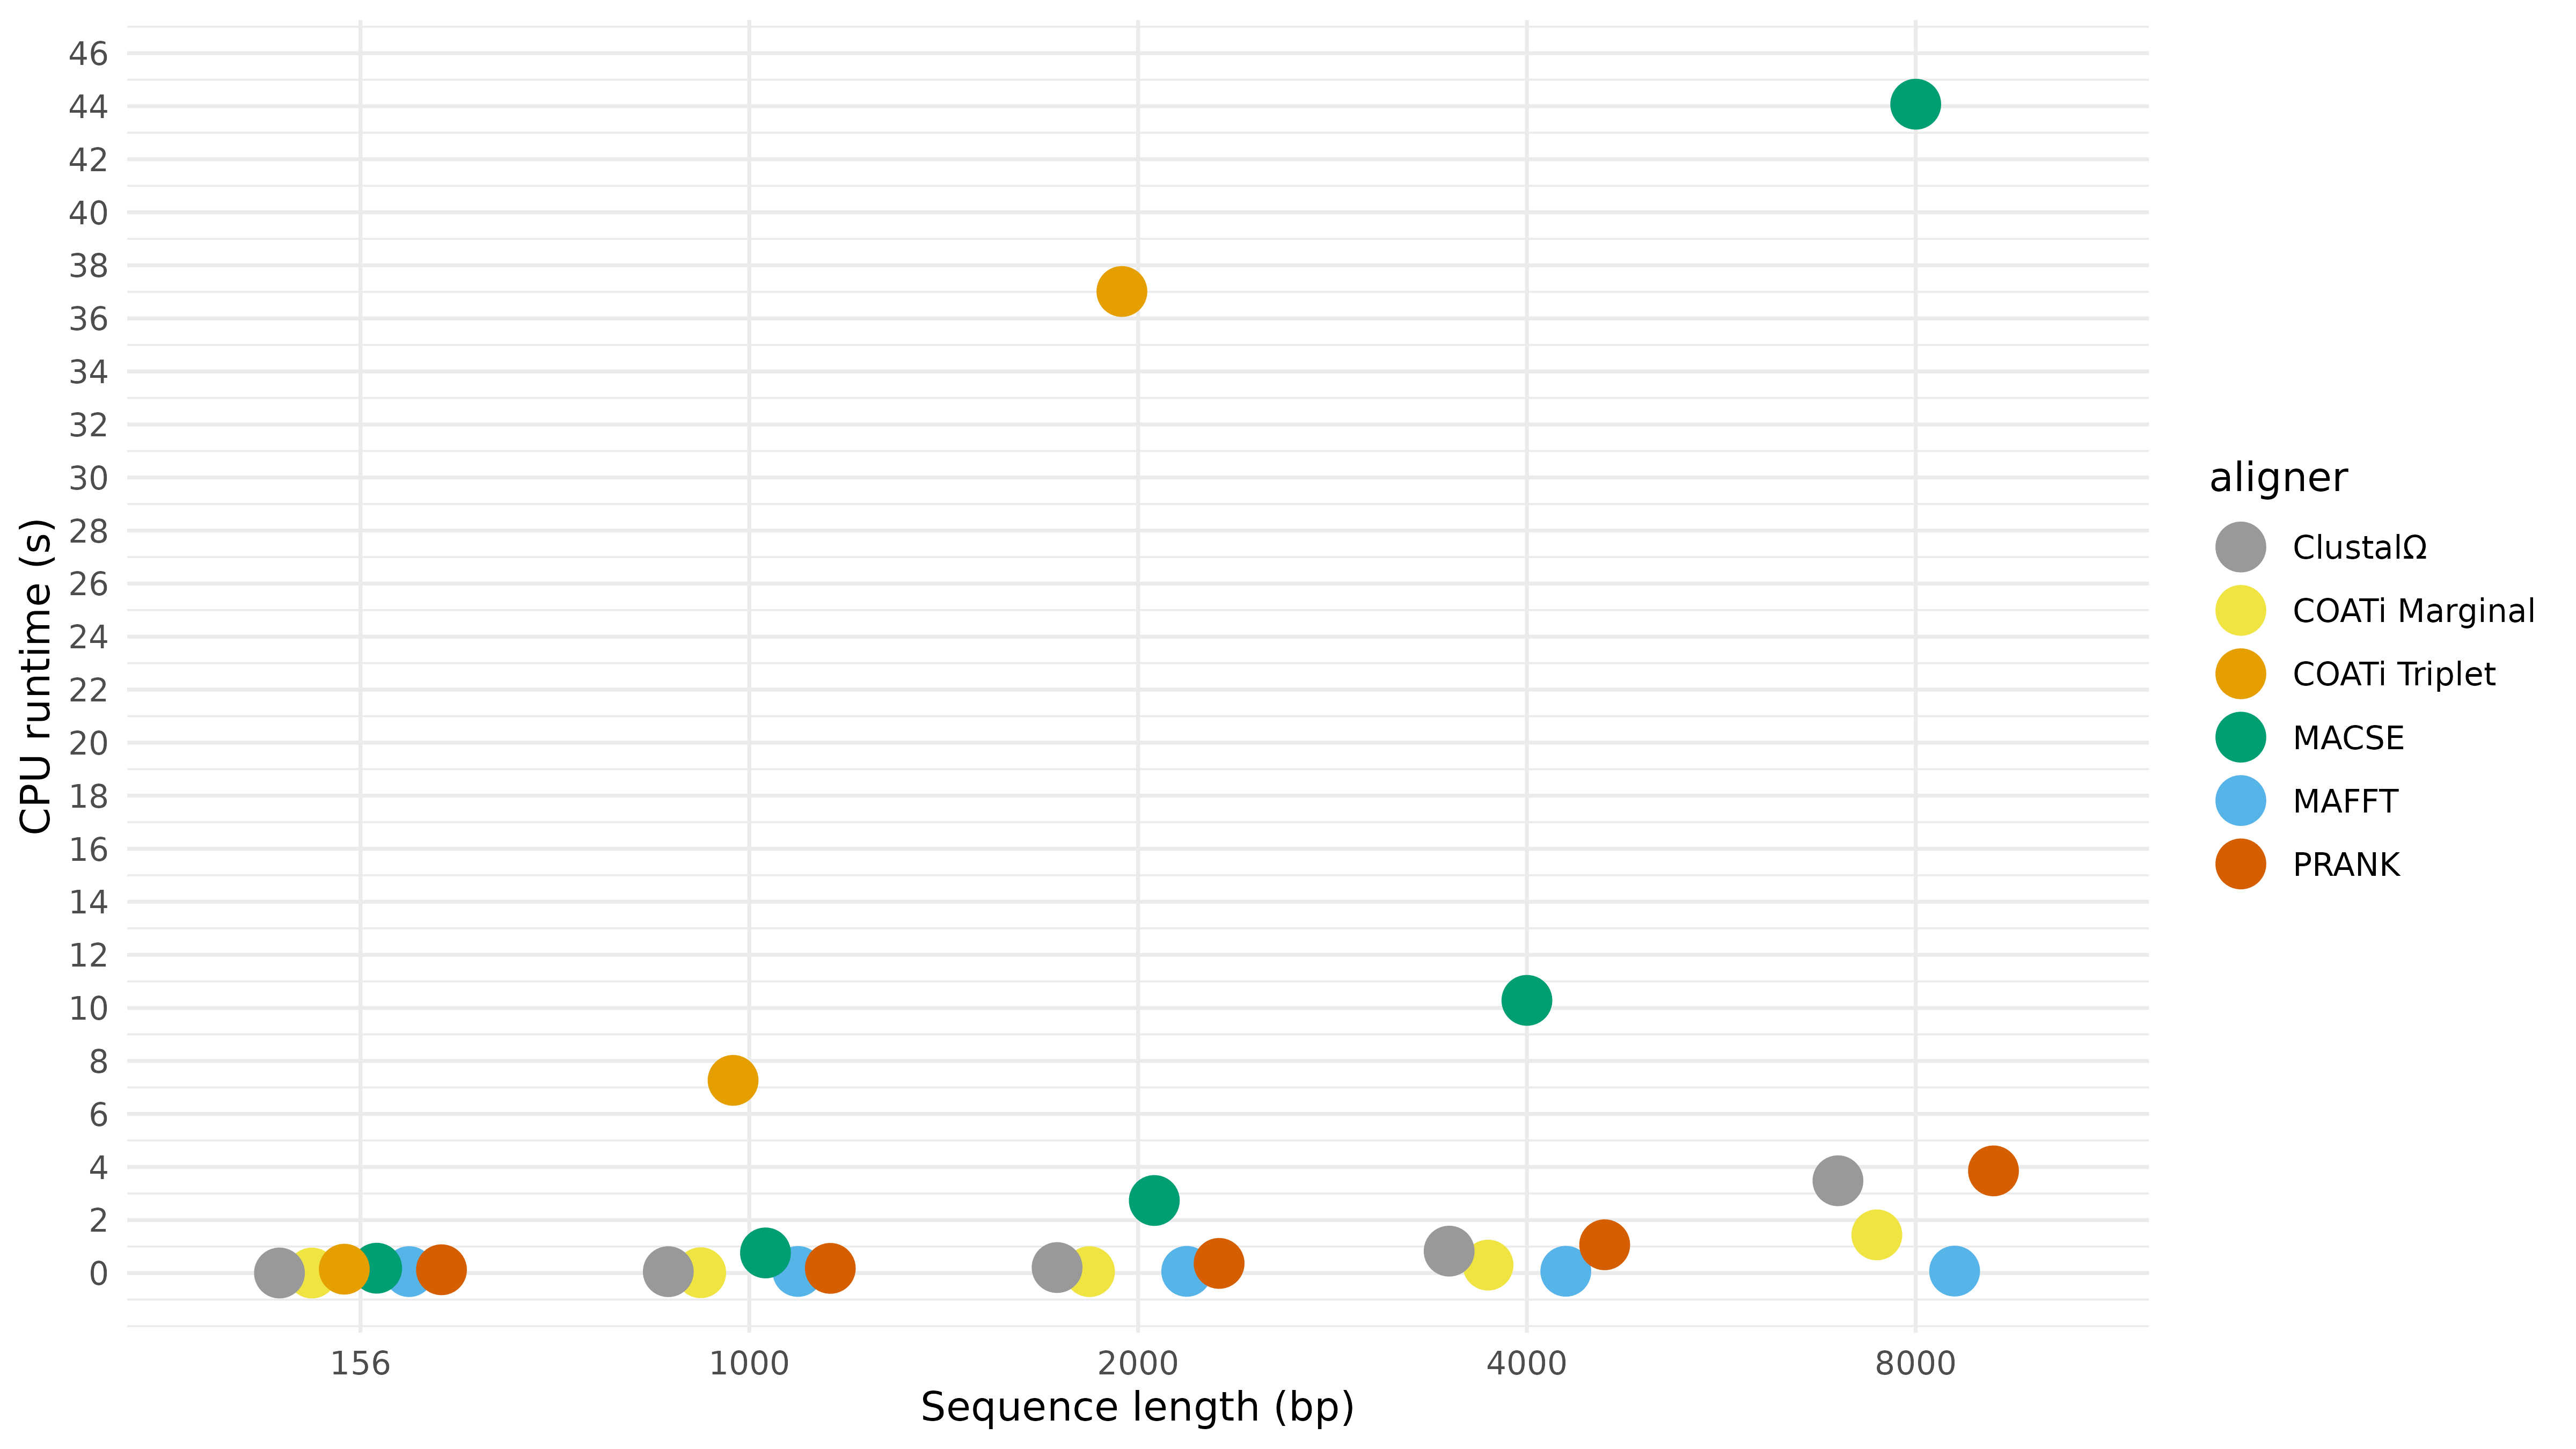
\includegraphics[height=0.95\textheight,center]{defense/images/runtime_aligners.png}
\end{frame} %-------------------------------------------------------------------

\begin{frame}{COATi Implementation} %-------------------------------------------
% \cyan{Modify this, probably shorten. Keep brief but highlight the software development work and that there exists a tool available to researchers already.}
% \begin{columns}
    % \column{0.6\textwidth}
    \begin{itemize}
	\setlength\itemsep{1em}
        \item Triplet alignment using FST operations from openFST library (C\texttt{++}).
        \item Marginal alignment adapted version of Gotoh dynamic programming algorithm.
        \item Optimizations and other procedures.
        \item Additional functionalities: sample, initial MSA, format, and genseed.
        \item Project has CI and code coverage on GitHub.
        \item Over 7,000 lines of C\texttt{++} code.
    \end{itemize}
    % \column{0.4\textwidth}
    % \begin{columns}
    %     \column{0.6\textwidth}
    %         \scalebox{0.6}{\newcommand{\cBlue}[1]{\textbf{\textcolor{blue}{#1}}}
\newcommand{\cPurple}[1]{\textbf{\textcolor{purple}{#1}}}
\newcommand{\cOrange}[1]{\textbf{\textcolor{orange}{#1}}}

\begingroup\centering
\begin{tabular}{c|c|c|c|c}
Codon & uchar & Position & Mask & uchar \& mask $\gg$ shift = Nucleotide\\
\hline
\cBlue{A}\cPurple{C}\cOrange{G} & 00 \cBlue{00} \cPurple{01} \cOrange{10} & 0 & 00 \textbf{11} 00 00 & 00 \cBlue{00} 00 00 $\gg$ 4 \hspace{0.8em}= \cBlue{00} (\cBlue{A})\\
\cBlue{A}\cPurple{C}\cOrange{G} & 00 \cBlue{00} \cPurple{01} \cOrange{10} & 1 & 00 00 \textbf{11} 00 & 00 00 \cPurple{01} 00 $\gg$ 2 \hspace{0.8em}= \cPurple{01} (\cPurple{C})\\
\cBlue{A}\cPurple{C}\cOrange{G} & 00 \cBlue{00} \cPurple{01} \cOrange{10} & 2 & 00 00 00 \textbf{11} & 00 00 10 \cOrange{00} $\gg$ 0 \hspace{0.8em}= \cOrange{10} (\cOrange{G})\\
\end{tabular}
\par\endgroup}
    % \end{columns}
% \end{columns}
\note[item]{openFST is a general purpose FST library written in C++.}
\note[item]{Unrefined initial MSA (work for future grad students in lab).}
\note[item]{During the last 2-3 years I've written about 7000 lines of code developing coati.}
\end{frame} %-------------------------------------------------------------------

\begin{frame}{Conclusion} %-----------------------------------------------------
\begin{itemize}
    \setlength\itemsep{1em}
    \item Sequence alignment is a fundamental problem in bioinformatics that is not fully solved.
    \item I developed a model and built an aligner for CDS that understands common artifacts in genomic data and outperforms available methods.
    \item Model and tool development must continue to evolve to handle the volume and characteristics of genomic data in the present age.
\end{itemize}
\note[item]{With this project I developed and built an aligner \textbf{that researcher are already using (!)}, that understands common artifacts in genomic data and outperforms available methods.}
\note[item]{In addition, I want to highlight that usually model and tool development are not in the spotlight in our field, it's important to continue improving them to properly handle the volume and characteristics of the data (and for more accurate results).}
\end{frame} %-------------------------------------------------------------------

\begin{frame}{Thank you - Gracias}
% pictures?
% in no particular order
\begin{itemize}
\begin{columns}
    \column{0.3\textwidth}    
        \item Reed Cartwright
        \item Banu Ozkan
        \item Jay Taylor
        \item Ted Pavlic
        \item Abigail Howell
        \item Ziqi Zhu
        \item Courtney Grigsby
        \item Adam Orr
    \column{0.3\textwidth} 
        \item Samantha Ortega-Hufana
        \item Marise \& José
        \item Sebastián
        \item Patrick Park
        \item Sid Kao
        \item Sean Kao
        \item Ortega-Hufana family
        \item Jonny \& SwimDevils
    \column{0.3\textwidth}    
        \item Henry Secaira
        \item Vanessa 
        \item Romain Dahan
        \item Tim Licknack
        \item Academic advisors
        \item The Carpentries
        \item Sergio García
        \item Volleyball crew
        % \item Erin and Spencer
\end{columns}
\end{itemize}
\note[item]{Thank everyone here for coming today and to the many people that have helped me through my journey (included but not limited to <list>).}
\end{frame} %-------------------------------------------------------------------

\begin{frame}{Questions} %------------------------------------------------------
% 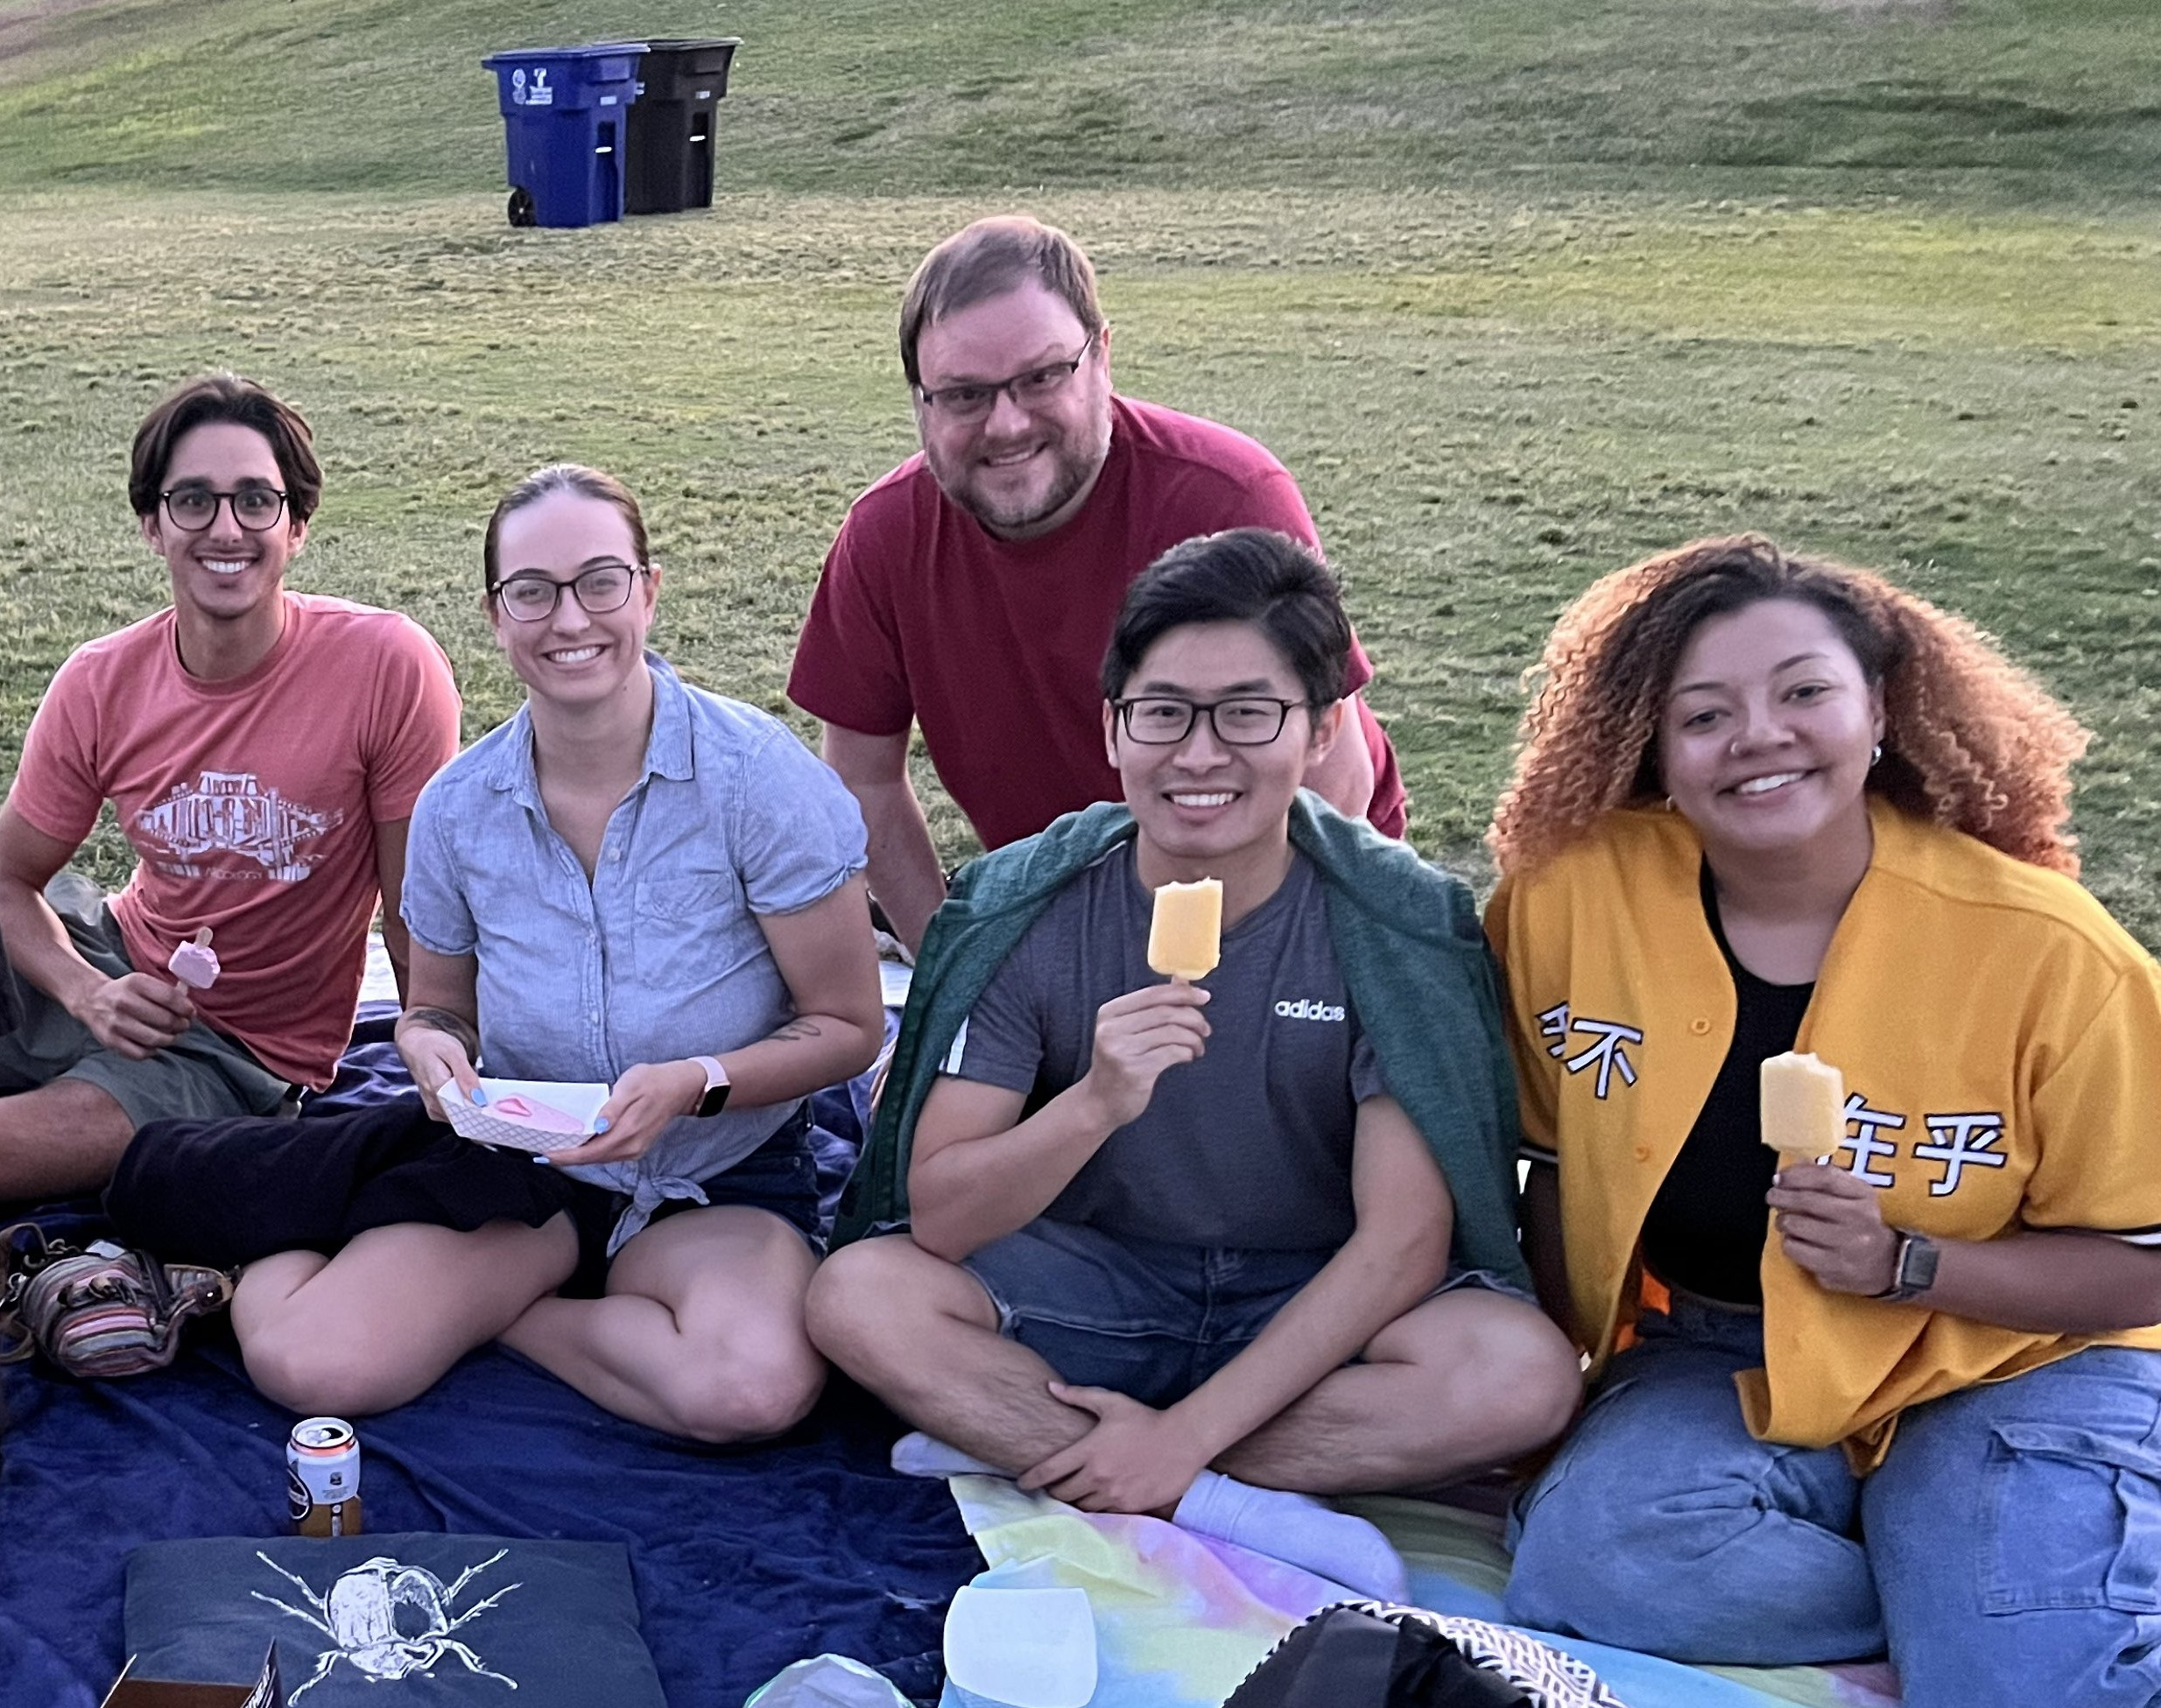
\includegraphics[scale=0.1,center]{images/lab.jpg}
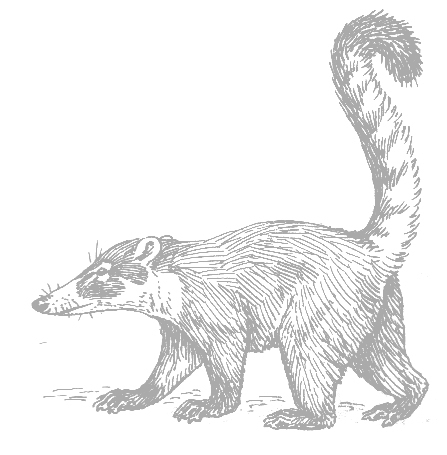
\includegraphics[center]{images/coati_psf_light.jpg}
\end{frame} %-------------------------------------------------------------------

% ##############################################################################
% \appendix % ####################################################################
% Supplemental slides

\begin{frame}[noframenumbering] %-----------------------------------------------
\centering
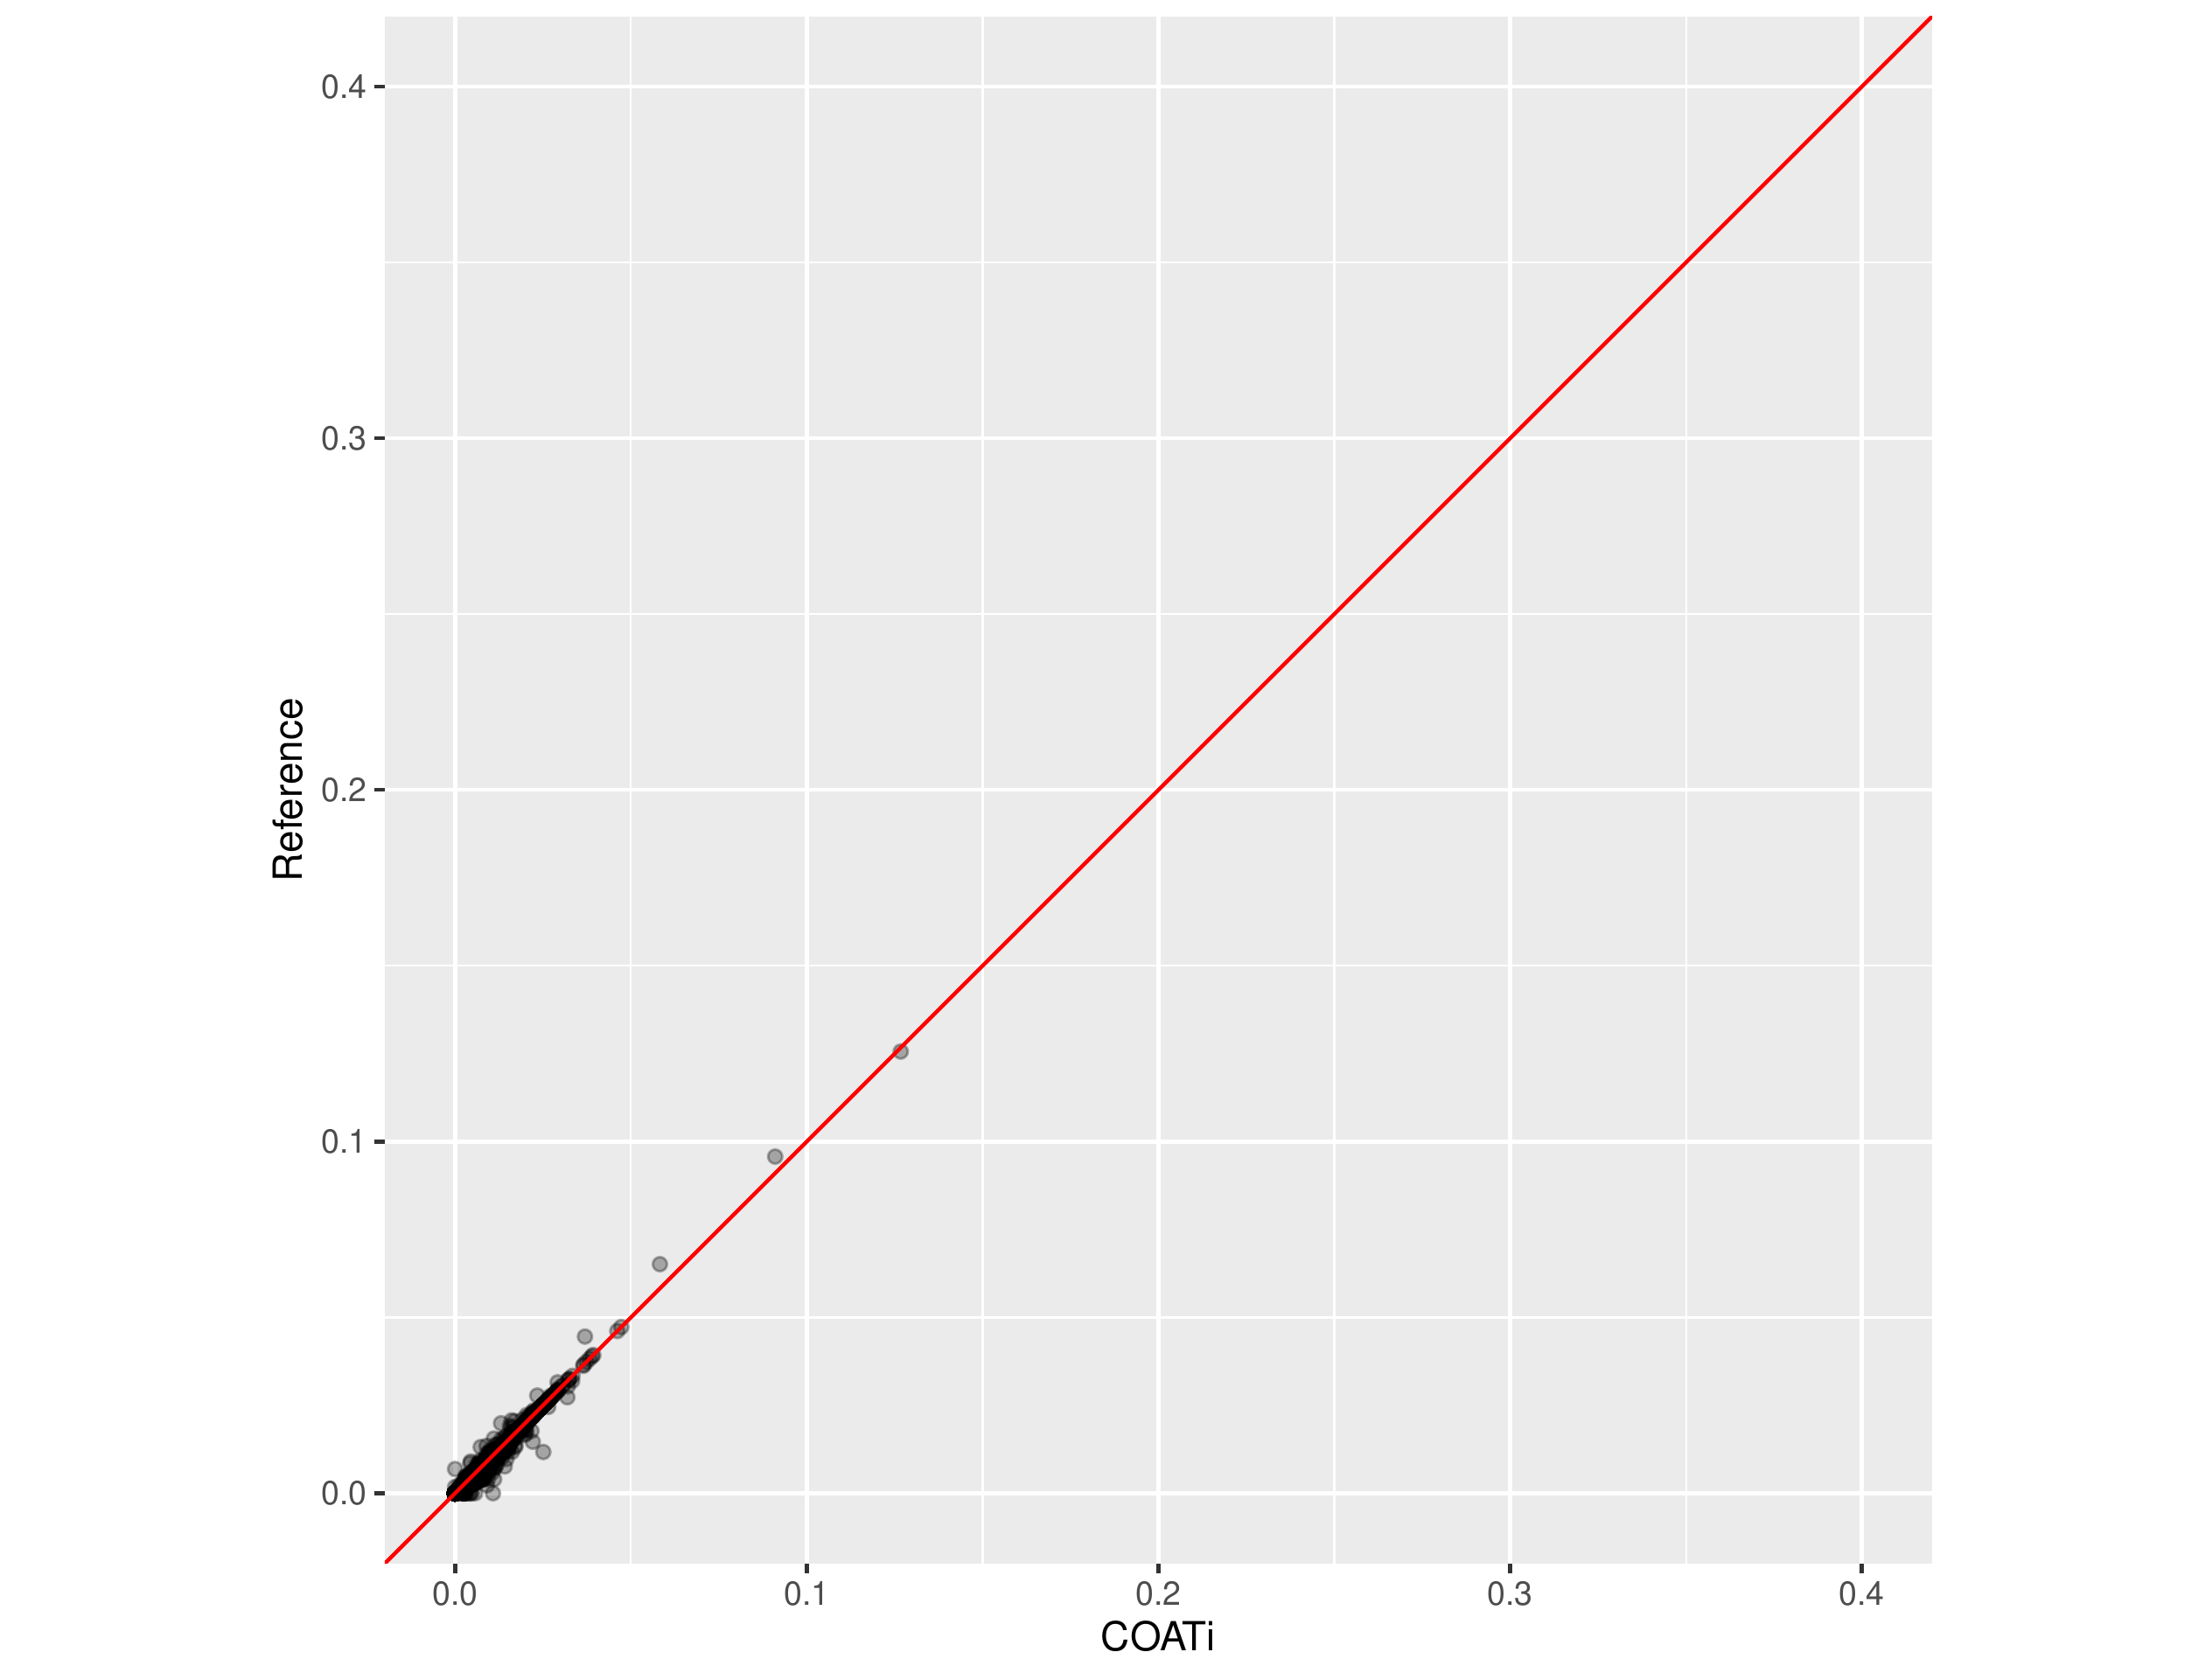
\includegraphics[height = \textheight]{defense/suppl/COATi_ref_distance.png}
\end{frame} %-------------------------------------------------------------------

\begin{frame}[noframenumbering] %-----------------------------------------------
\begin{columns}
    \column{0.5\linewidth}
        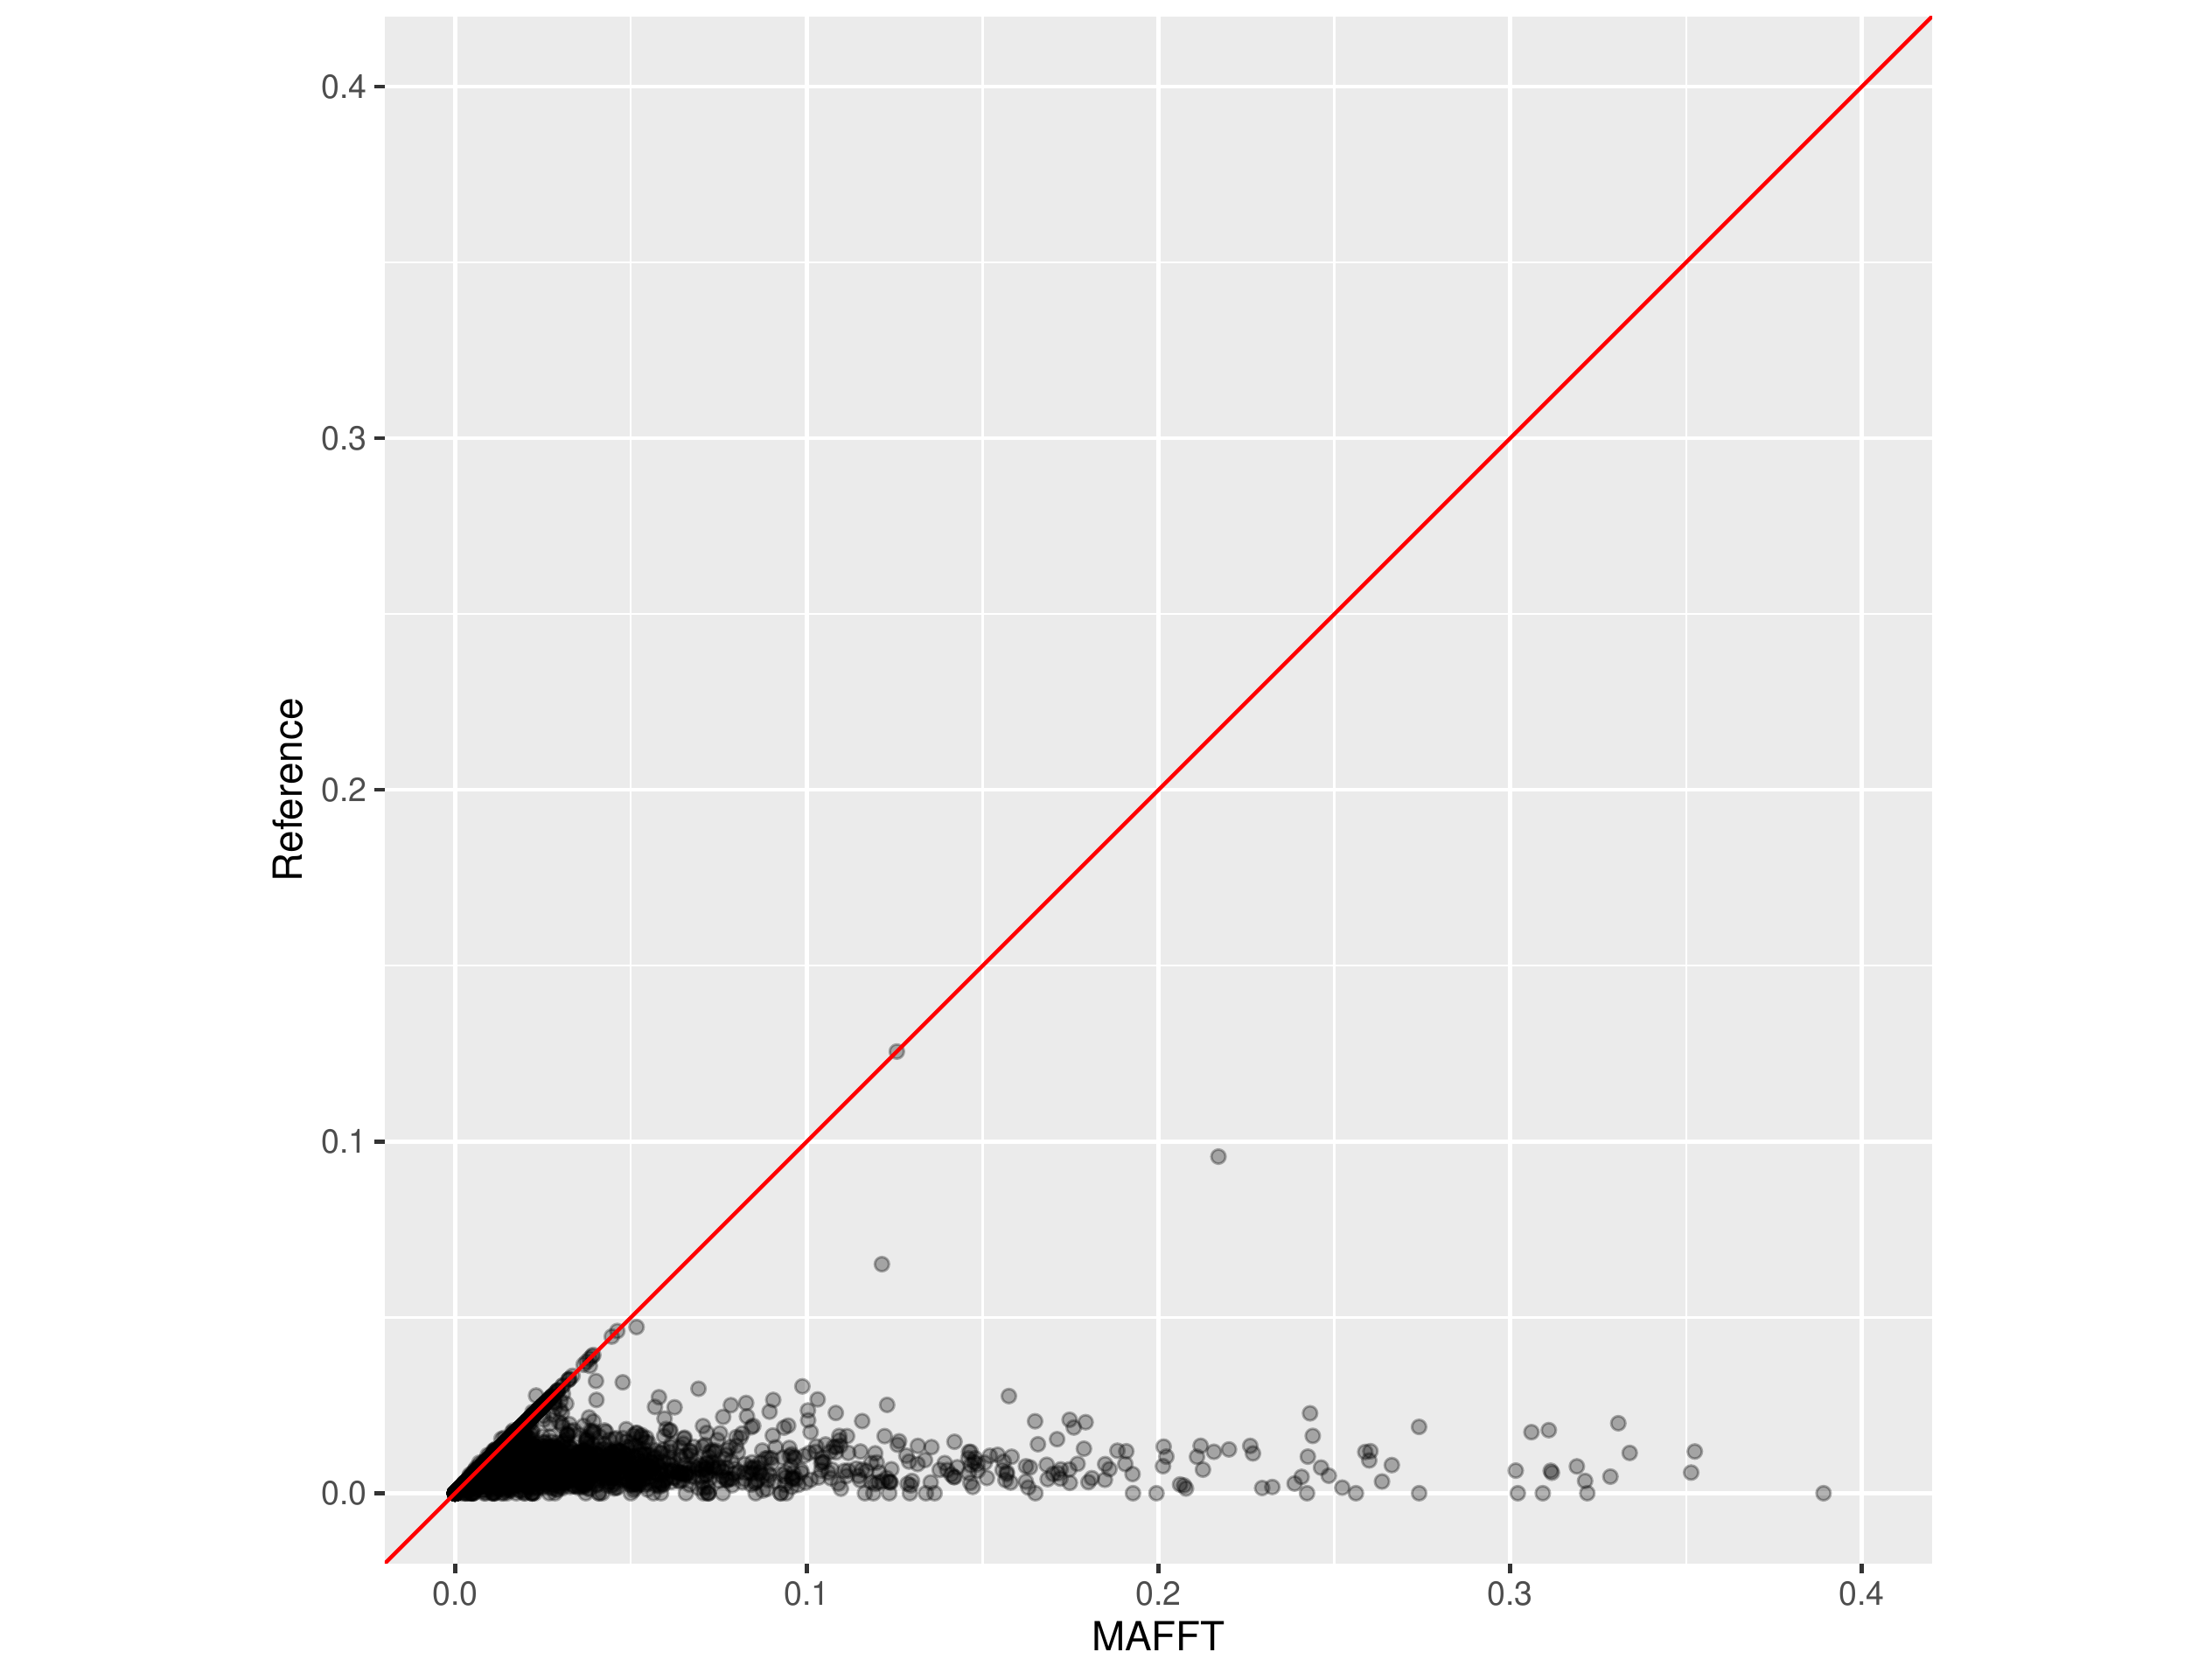
\includegraphics[width = \textwidth, trim={2.5cm 0 3cm 0}, clip]{defense/suppl/MAFFT_ref_distance.png}
    \column{0.5\linewidth}
        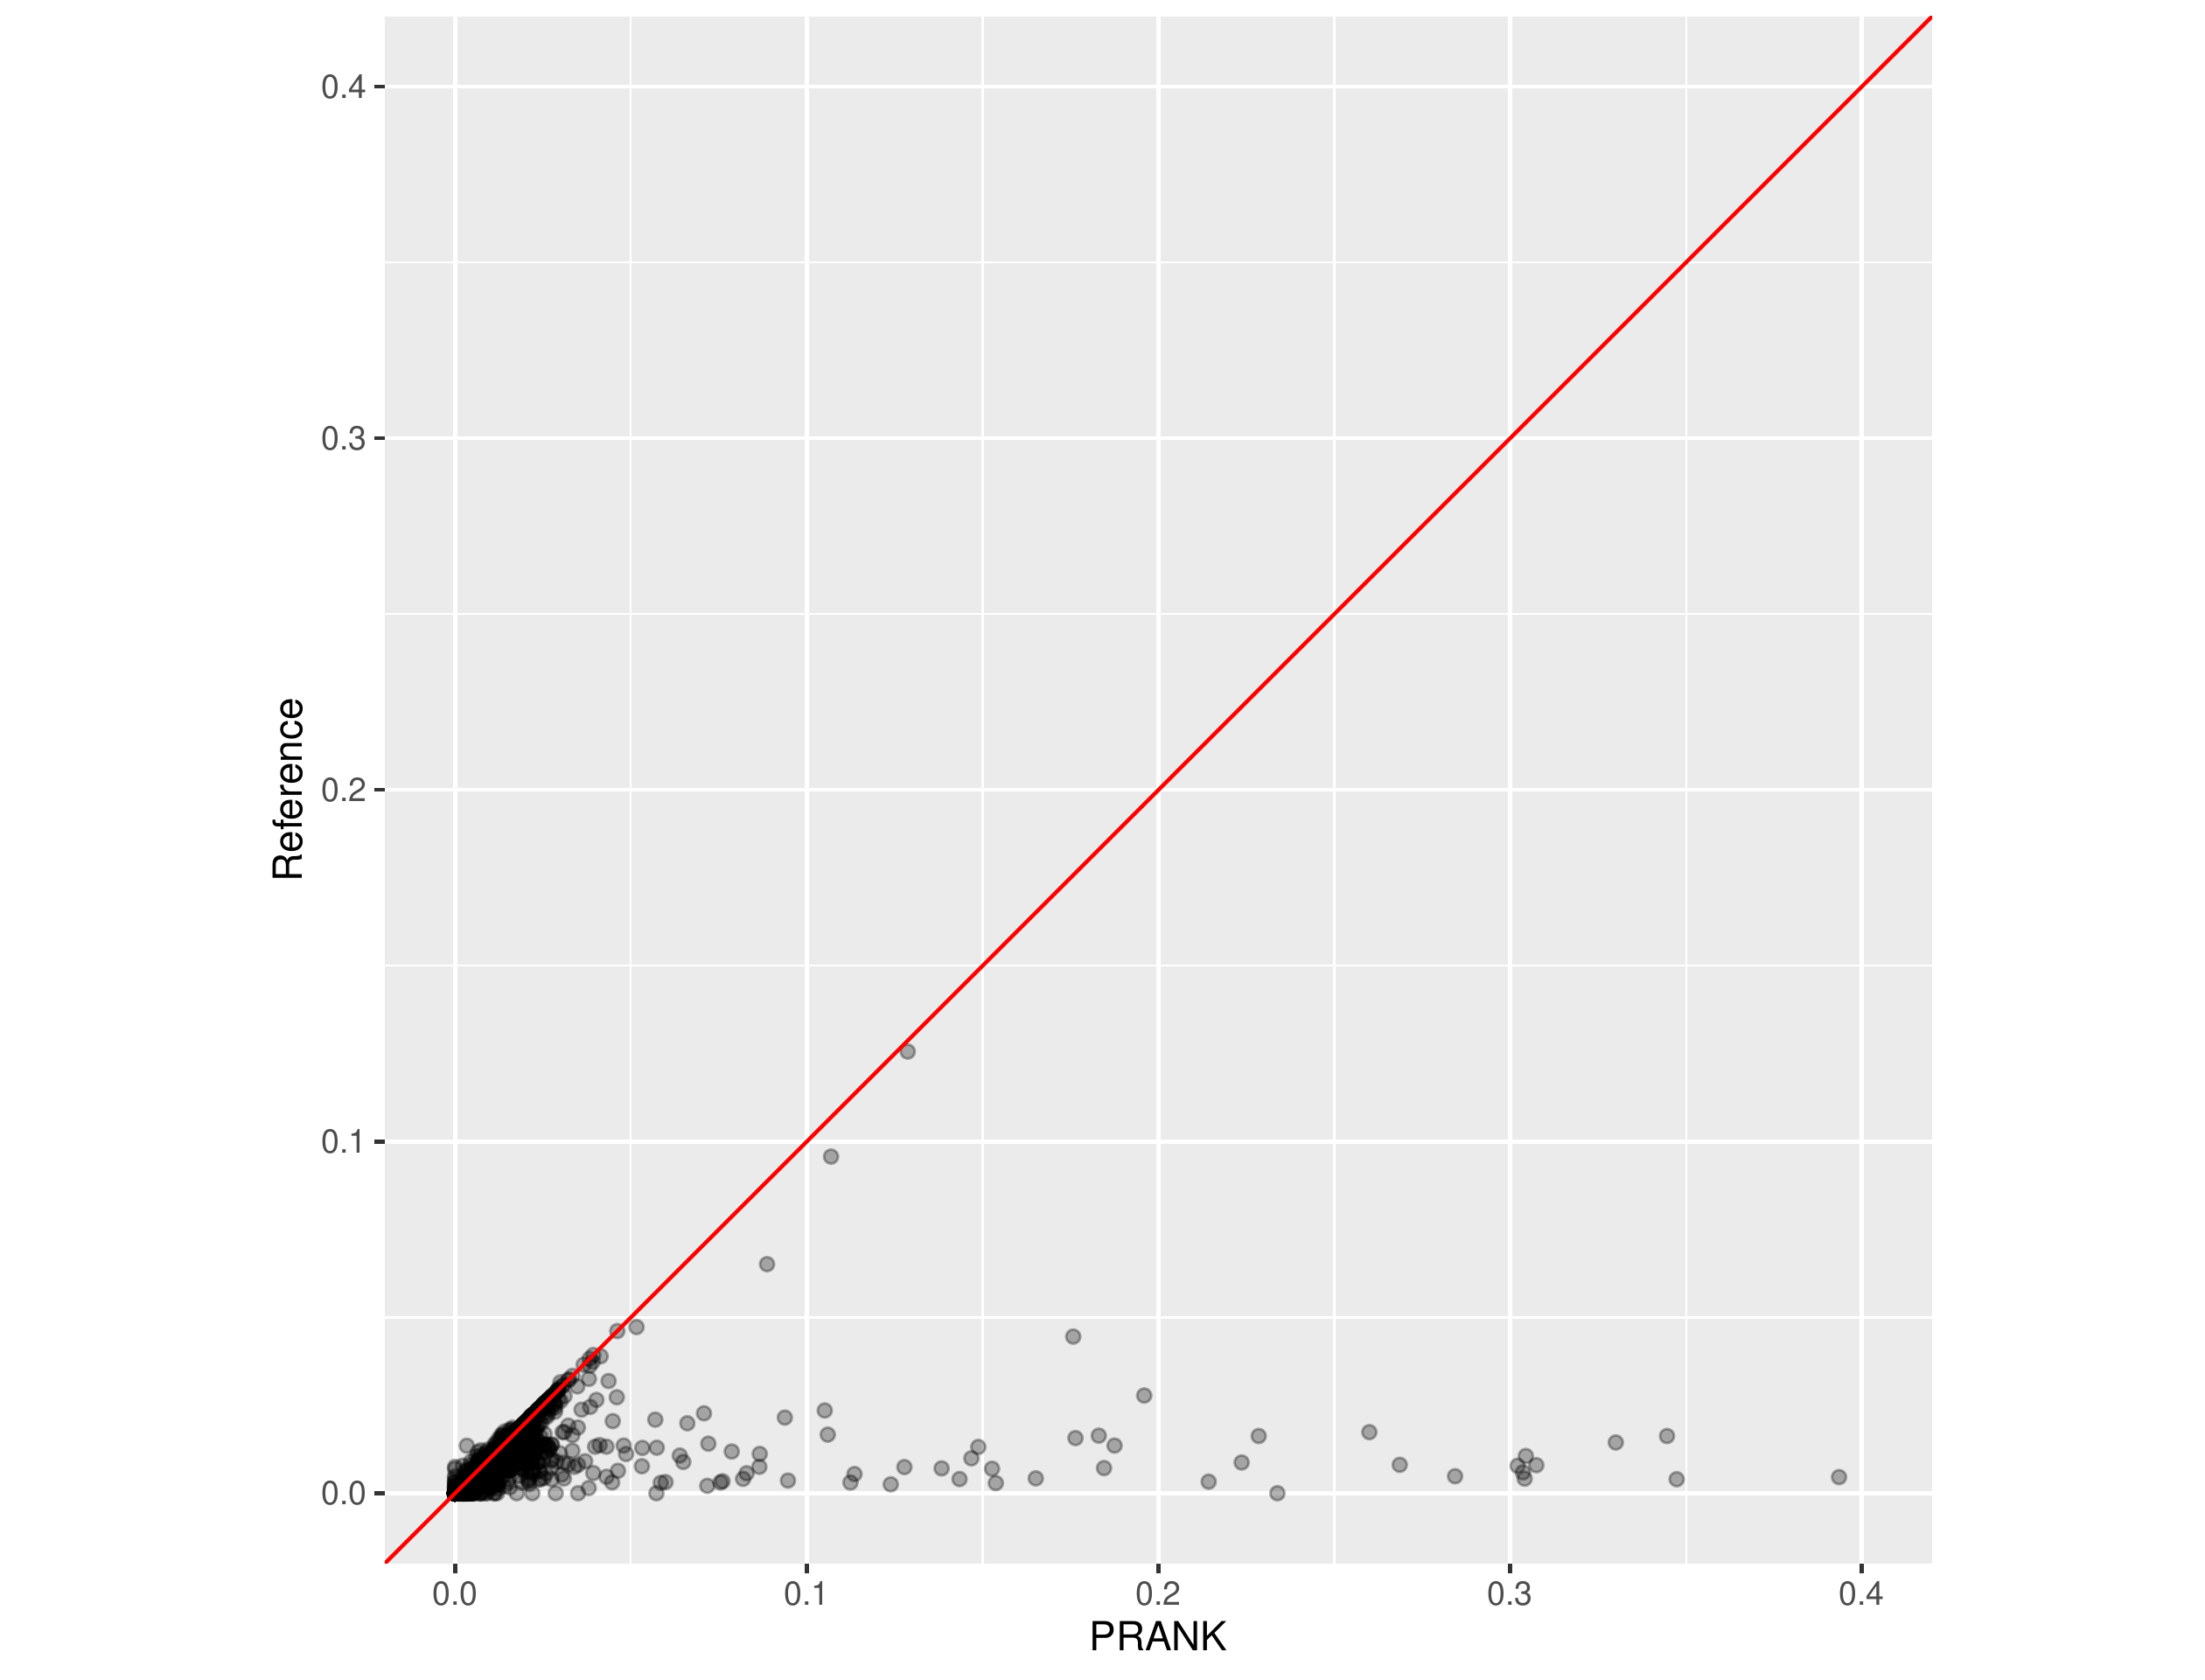
\includegraphics[width = \textwidth, trim={2.5cm 0 3cm 0}, clip]{defense/suppl/PRANK_ref_distance.png}
\end{columns}
\end{frame} %-------------------------------------------------------------------

\begin{frame}[noframenumbering] %-----------------------------------------------
\begin{columns}
    \column{0.5\textwidth}
        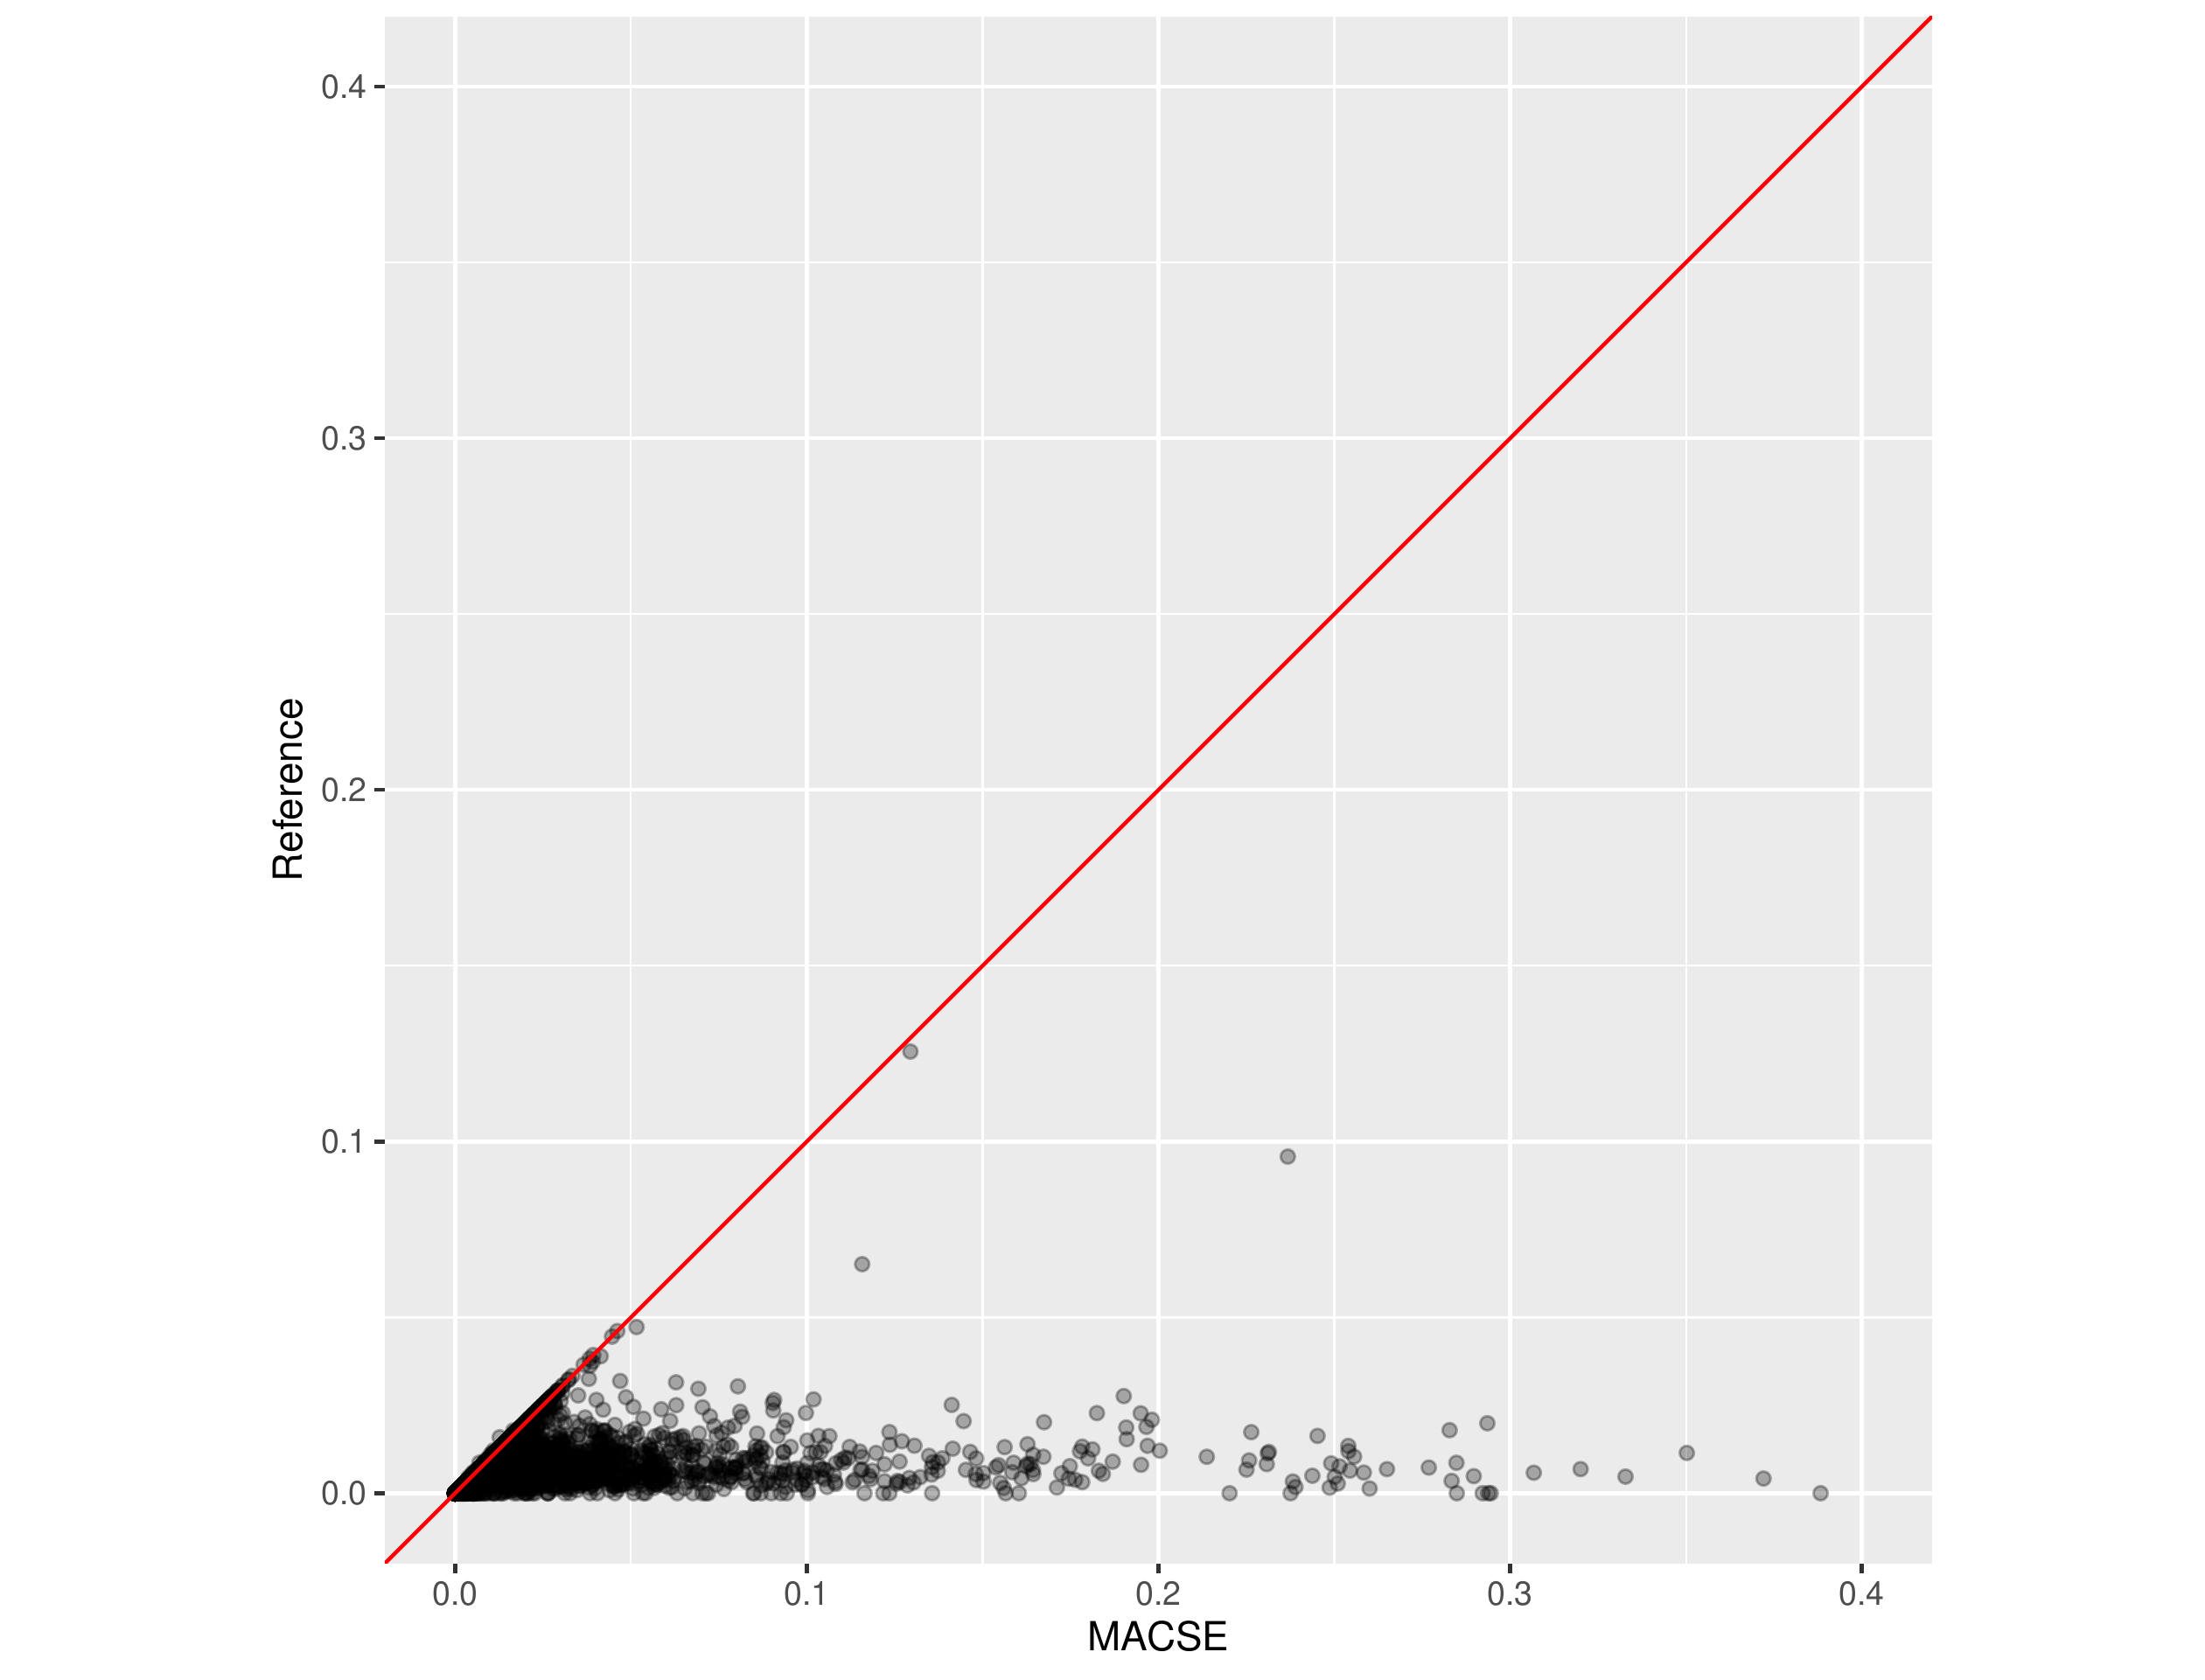
\includegraphics[width = \textwidth, trim={2.5cm 0 3cm 0}, clip]{defense/suppl/MACSE_ref_distance.png}
    \column{0.5\textwidth}
        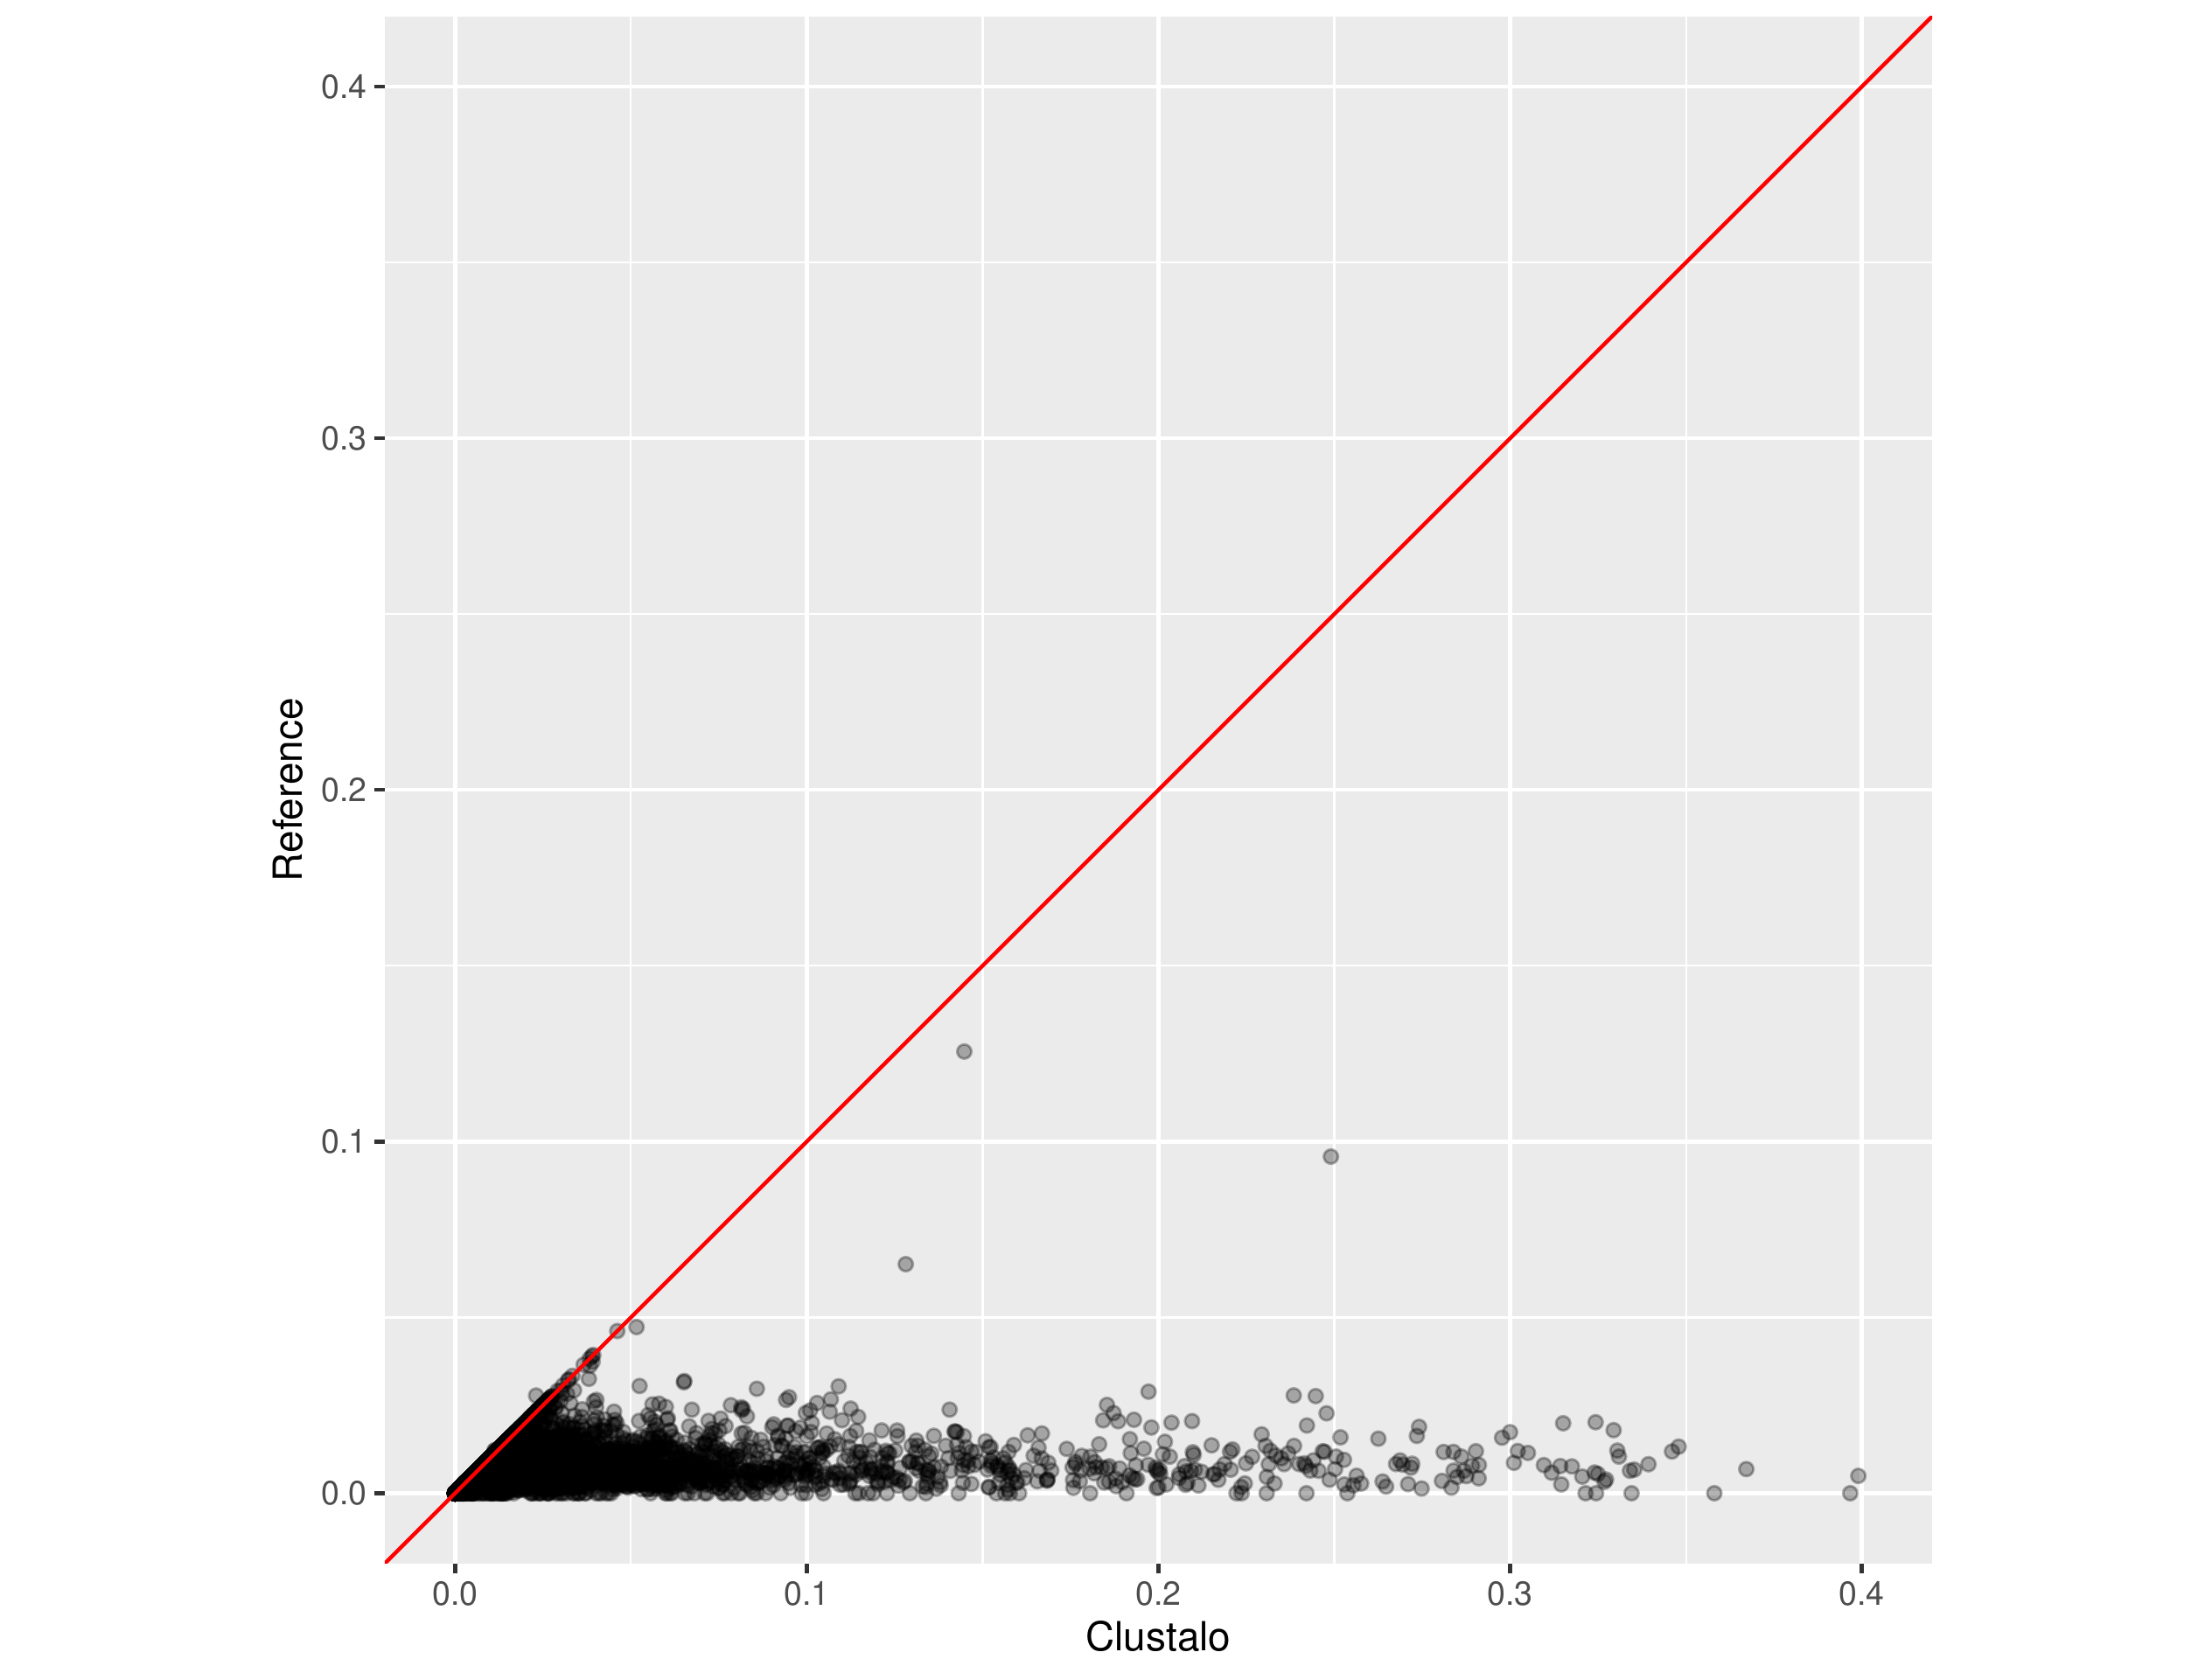
\includegraphics[width = \textwidth, trim={2.5cm 0 3cm 0}, clip]{defense/suppl/Clustalo_ref_distance.png}
\end{columns}
\end{frame} %-------------------------------------------------------------------

\begin{frame}[c,noframenumbering]{Substitution Model Parameters} %--------------
\centering
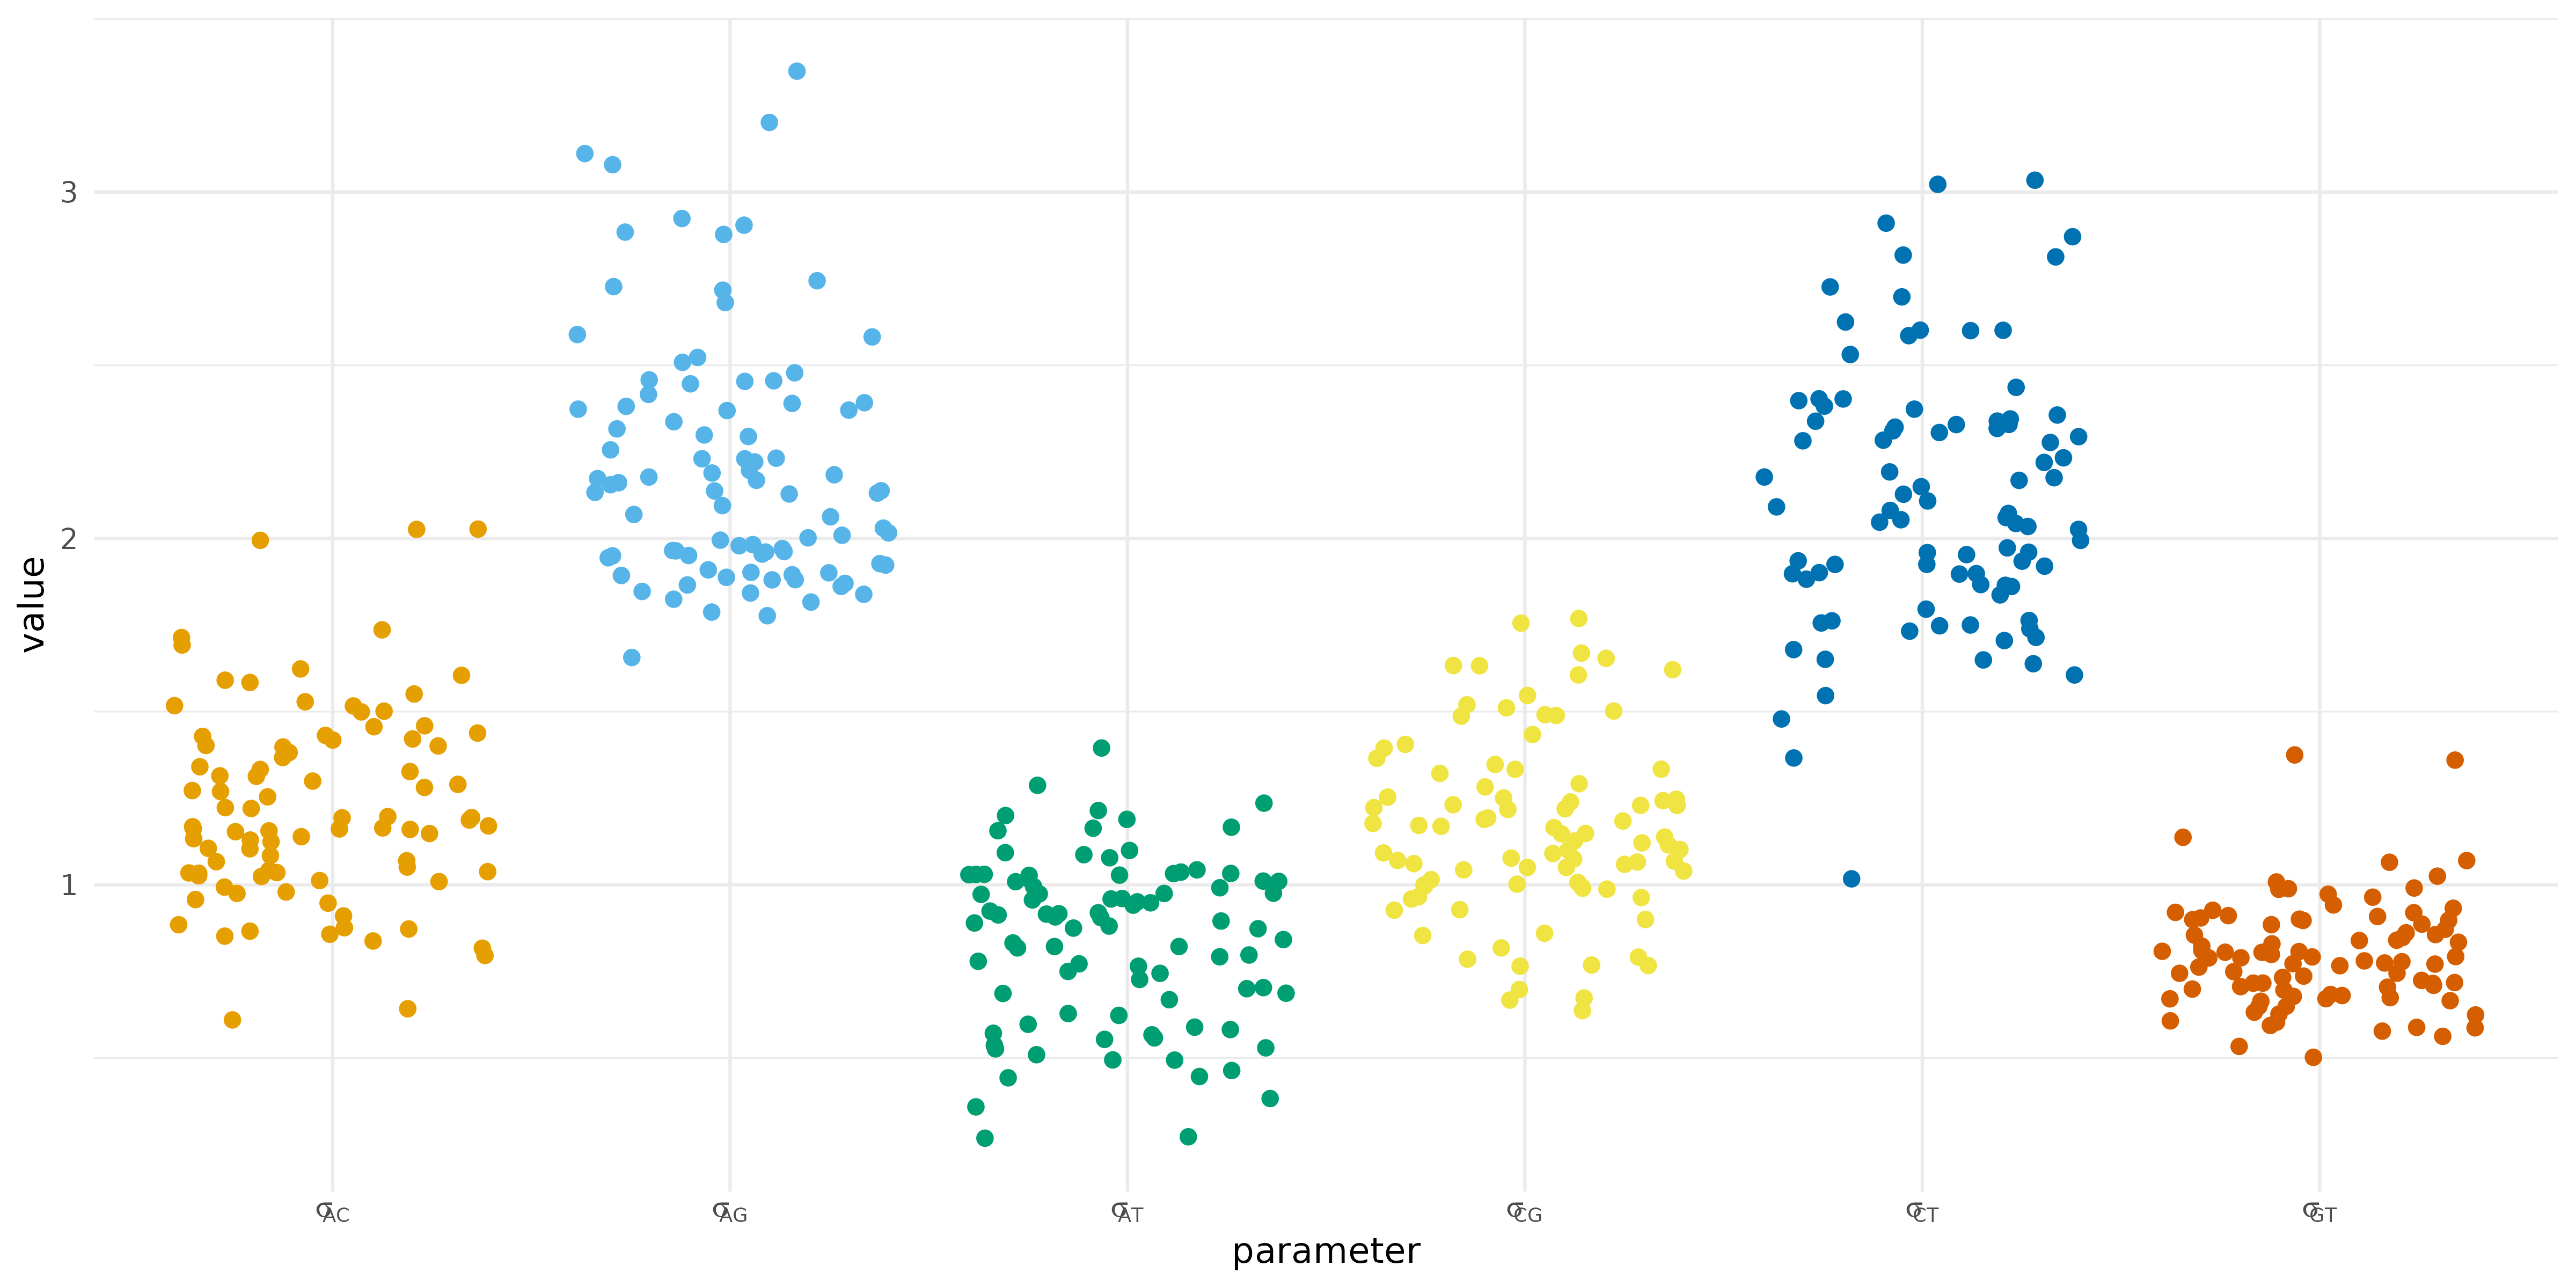
\includegraphics[height = 0.8\textheight]{defense/images/sigma_estimates_90_species.png}
\end{frame} %-------------------------------------------------------------------

\begin{frame}{Results---max} %--------------------------------------------------
\centering
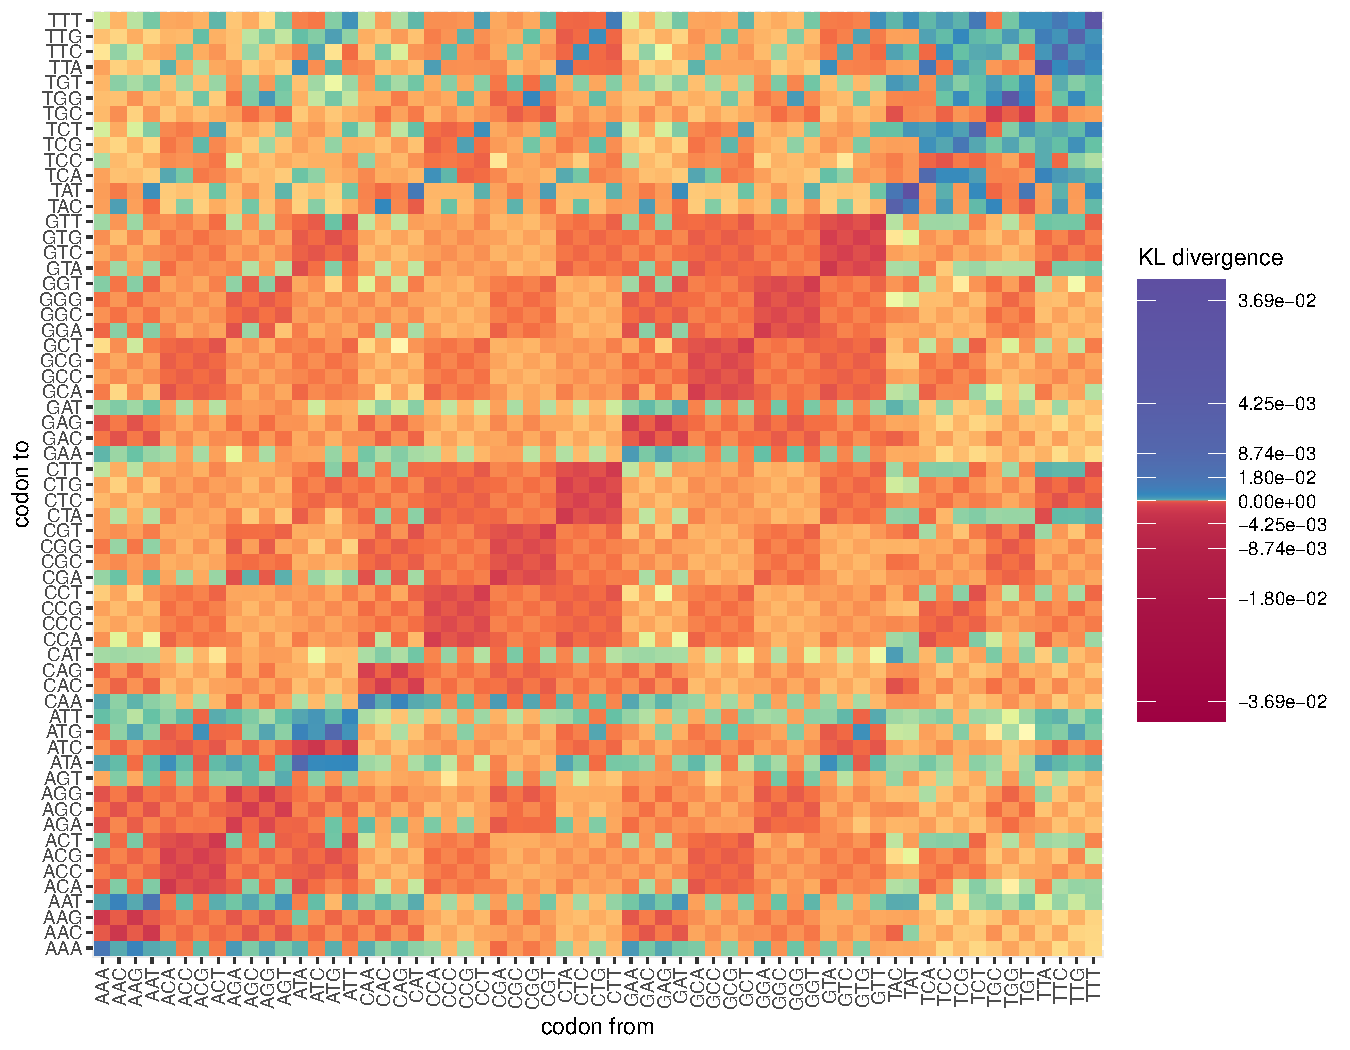
\includegraphics[height = 0.9\textheight]{chapter3/figures/heatmaps/tri-max-mg-1.pdf}
\end{frame} %-------------------------------------------------------------------

\begin{frame}{Results---sum} %--------------------------------------------------
\centering
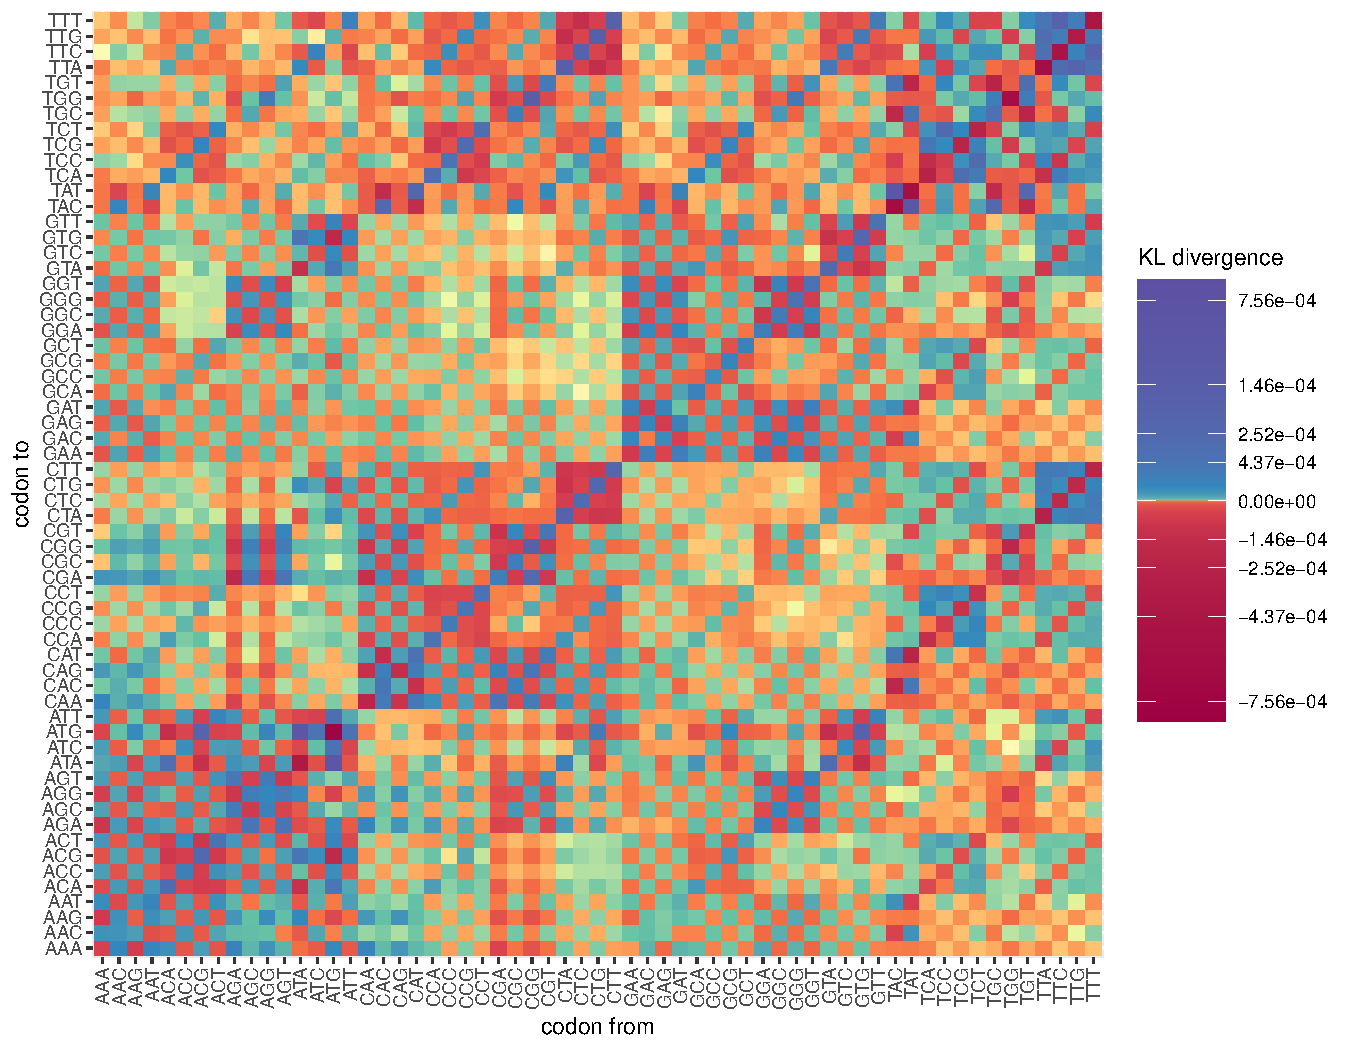
\includegraphics[height = 0.9\textheight]{chapter3/figures/heatmaps/tri-sum-mg-1.pdf}
\end{frame} %-------------------------------------------------------------------

\begin{frame}[noframenumbering] %-------------------------------------------------
\begin{columns}
\column{0.5\textwidth}
Non-negative function, $d(x,y)$, metric conditions:
\begin{itemize}
	\item $d(x,y) = 0$ iff $x=y$
	\item $d(x,y) = d(y,x)$ symmetry
	\item $d(x,z) \leq d(x,y) + d(y,z)$ triangle inequality
\end{itemize}
\column{0.5\textwidth}
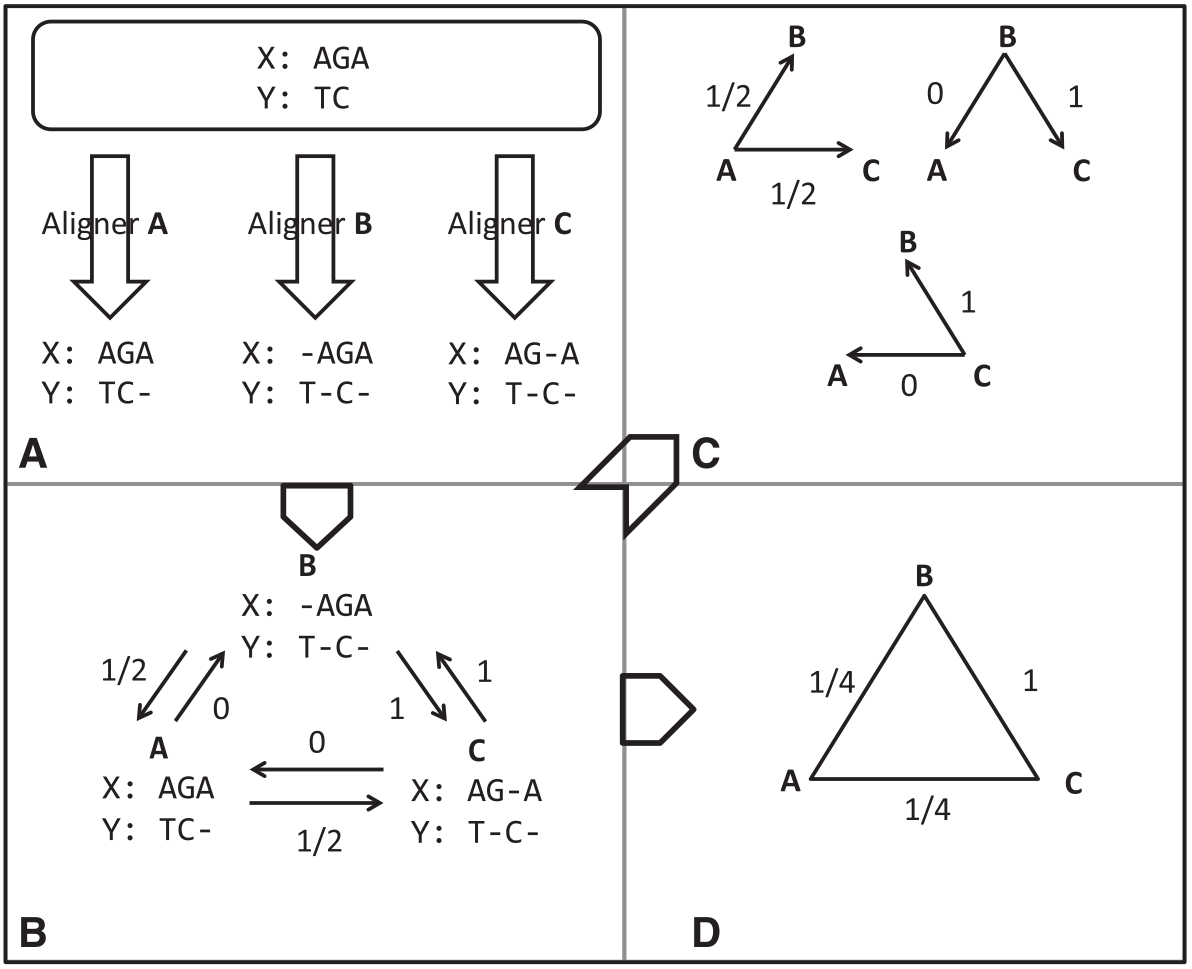
\includegraphics[scale=0.15,center]{./images/fig-sop-problems.png}
\end{columns}
% \footnotetext[1]{\cite{metrics_blackburne_whelan_2011}}
\note[item]{For a function to be a valid metric has to meet all three criteria
	(explain briefly). Sum of pairs, a common score used to evaluate differences
	between MSA based on the number of matches on each column, has been proven
	to not satisfy all 3 conditions. An example (fig).}
\end{frame} %---------------------------------------------------------------------

\begin{frame}[noframenumbering] %-------------------------------------------------
\begin{align*}
d(A,B) = \frac{1}{c} \sum_i \sum_j d(A,B)^i_j = \frac{1}{c} \sum_i \sum_j \frac{|H(A)^i_j \triangle H(B)^i_j|}{|H(A)^i_j|+|H(B)^i_j|}
\end{align*}

\note[item]{Homology set: characters on the same column, i.e. nucleotides said to
	be homologous.}
\note[item]{Hamming distance: number of different positions or minimum number of
	substitutions required to change one set into the other.}
\end{frame} %-------------------------------------------------------------------

\begin{frame}[noframenumbering] %-----------------------------------------------
\centering{\resizebox{0.85\linewidth}{!}{% Resize table to fit within \linewidth horizontally
\begingroup\centering
\begin{tabular}{cccccccc|cccccccc}
A & A & T & A & T & T & G & - & A & A & T & A & T & T & - & G \\
A & - & - & A & T & T & A & G & A & A & T & - & - & T & A & G \\
A & - & - & A & - & T & A & G & A & A & - & - & - & T & A & G \\
\end{tabular}
\par\endgroup

}}

\vspace{1em}
\begin{columns}
\column{0.5\textwidth}
$d_{seq}(A,B)^1_1=0$ \\
$d_{seq}(A,B)^2_1=0$ \\
$d_{seq}(A,B)^3_1=0$ \\
\column{0.5\textwidth}
$d_{seq}(A,B)^1_2=\frac{2}{4}=\frac{1}{2}$ \\
$d_{seq}(A,B)^2_2=\frac{1}{4}$ \\
$d_{seq}(A,B)^3_2=\frac{1}{4}$ \\
\end{columns}
\end{frame} %-------------------------------------------------------------------

\begin{frame}[noframenumbering] %-----------------------------------------------
Codon substitution with instantaneous substitution rate matrix $Q$:
\vspace{1em}
\begin{align*} Q_{ij} &= \begin{cases}
    \mu_{ij} & \text{if $i$ and $j$ are synonymous}\\
    \omega \cdot \mu_{ij} & \text{if $i$ and $j$ are nonsynonymous}
    \end{cases}\\[10pt]
   Q_{ii} &= -\sum_{j:j \neq i} Q_{ij}
\end{align*}
\begin{itemize}
	\item $\mu_{ij}$: mutation rate of codon $i$ to $j$.
	\item $\omega$: coefficient of selection.
	\item Supports a variety of models %(e.g.
		%MG94\parencite{muse_gaut_1994}, ECM\parencite{kosiol_ECM_2007}).
	% \item $t$: evolutionary time.
	% \item $P(j | i;t) = {\rm e}^{Qt}$.
\end{itemize}
\end{frame} %-------------------------------------------------------------

\begin{frame}{Needleman-Wunsch} %-----------------------------------------------
\textbf{Dynamic programming} algorithm to find the highest scoring alignment.\\
Solves a large problem by finding optimal solutions to smaller problems.
\begin{columns}
    \column{0.6\textwidth}
        \begin{algorithmic}[1]
        \State \textbf{Insert} gap penalties
        \State \textbf{Fill} matrix
            \For{$i \gets 1$ to $n$}
                \For{$j \gets 1$ to $m$}
                    \State \textbf{Compute} deletions
                    \State \textcolor{blue}{mch} = NW[i-1, j-1] + \text{score}($s_i$, $v_j$)
                    \State \textcolor{green}{del} = NW[i-1, j] + $\alpha$
                    \State \textcolor{red}{ins} = NW[i, j-1] + $\alpha$
                    \State NW[i, j] = \text{max}(mch, del, ins)
                \EndFor
            \EndFor
        \end{algorithmic}
    \column{0.4\textwidth}
        \begin{tikzpicture}
        % Nodes for the matrix
        \foreach \i in {0,...,2}
            \node[anchor=east] at (-0.5,\the\numexpr2-\i\relax) {s$_\i$};
        \foreach \i in {0,...,2}
            \node[anchor=north] at (\i,3) {v$_\i$};
        
        \node at (-0.75, -1) {$\vdots$};
        \node at (3, 2.75) {$\cdots$};
        
        % Fill in the matrix
        \foreach \i in {0,1,2}
            \foreach \j in {0,1,2}
                \node[draw,minimum width=1cm,minimum height=1cm] at (\i,\j) {};
        
        \draw[->,thick,blue] (0,2) -- (0.90,1.1);
        \draw[->,thick,red] (0,1) -- (0.90,1);
        \draw[->,thick,green] (1,2) -- (1,1.1);
        \end{tikzpicture}
\end{columns}
\end{frame} %-------------------------------------------------------------------

\begin{frame}{Marginal Model Alignment} %---------------------------------------
\begin{itemize}
    \item Limitation of Needleman-Wunsch (NW): linear gap penalty ($l \cdot \alpha$).
    \item Gotoh algorithm: NW with affine gap penalties ($\alpha + (l - 1) \cdot \beta$).
    \item COATi marginal alignment adapts Gotoh.
\end{itemize}
\begin{columns}
    \column{0.5\textwidth}
\begin{align*}
    D_{i,j} &= + \begin{cases}
        M_{i-1, j} \times \log_{1m}(g)\\
        D_{i-1, j} \times e\\
        I_{i-1, j} \times \log_{1m}(e) \otimes g\\
    \end{cases}\\
    I_{i,j} &= + \begin{cases}
        M_{i ,j-1} \times g\\
        I_{i, j-1} \times e\\
    \end{cases}\\
    M_{i,j} &= + \begin{cases}
        % s = P_{mar}[z_jx_i, z_j; \theta] \\
        M_{i-1, j-1} \times \log_{1m}(g) \times (1-g) \times s\\
        D_{i-1, j-1} \times \log_{1m}(e) \times s\\
        I_{i-1, j-1} \times \log_{1m}(e) \times \log_{1m}(g) \times s\\
    \end{cases}\\
\end{align*}
    \column{0.5\textwidth}
    \centering
    \resizebox{\textwidth}{!}{
%\documentclass{article}
% \documentclass[tikz]{standalone}

% \usepackage{pgf}
% \usepackage{tikz}
% \usetikzlibrary{arrows,automata,positioning}
% %\usepackage[latin1]{inputenc}
% \usepackage{verbatim}
% \usepackage{graphicx}

% \usetikzlibrary{shapes,arrows,positioning}
% \tikzset{
%   font={\fontsize{9pt}{11}\selectfont}
% }

\definecolor{colorR}{RGB}{228,26,28}    % RED
\definecolor{colorB}{RGB}{55,126,184}   % BLUE
\definecolor{colorG}{RGB}{77,175,74}    % GREEN
\definecolor{colorP}{RGB}{152,78,163}   % PURPLE
\definecolor{colorO}{RGB}{255,127,0}    % ORANGE
\definecolor{colorY}{RGB}{255,255,51}   % YELLOW
\definecolor{colorBn}{RGB}{166,86,40}   % BROWN
\definecolor{colorPk}{RGB}{247,129,191} % PINK
\definecolor{colorGy}{RGB}{153,153,153} % GRAY

% \begin{document}

\begin{tikzpicture}[->,>=stealth',shorten >=1pt,auto,node distance=6cm,ultra thick]
  \tikzstyle{every node}=[font=\large]

  \node[circle,fill=colorG!50,minimum size=1cm]  (S)					  {\textbf{Start}};
  \node[circle,fill=colorB!50,minimum size=1cm]	 (M) [right=20mm of S]  {\textbf{M}};
  \node[circle,fill=colorB!50,minimum size=1cm]  (I) [above right of=M] {\textbf{I}};
  \node[circle,fill=colorR!50,minimum size=1cm]  (E) [below right of=M] {\textbf{End}};
  \node[circle,fill=colorB!50,minimum size=1cm]  (D) [below right of=I] {\textbf{D}};

  \path (S) edge 			  node {}	(M)
  		(M) edge [out=265,in=200,looseness=10]  node [midway,font=\large] {x$_\text{i}$:z$_\text{j}$ /$(1-\text{g})^2\cdot $s} (M)
  			edge [bend left]  node [font=\large] {\O:z$_\text{j}$/g} (I)
            edge         node [font=\large] {x$_\text{i}$:\O/ $(1-\text{g})\cdot$ g} (D)
            edge [bend right] node [font=\large] {$(1-\text{g})^2$}	(E)
        (I) edge [out=120,in=60,looseness=10] node [font=\large] {\O:z$_\text{j}$/ e} (I)
            edge [bend left]  node [rotate=50, above=1em, font=\large] {x$_\text{i}$:z$_\text{j}$/ $(1-\text{e})\cdot (1-\text{g}) \cdot$ s} (M)
            edge [bend left] node [font=\large] {x$_\text{i}$:\O/ $(1-\text{e}) \cdot$ g} (D)
            edge [bend left] node [pos=0.96, rotate=60, right=1.5em, font=\large] {$(1-\text{e}) \cdot (1-\text{g})$} (E)
        (D) edge [out=30,in=330,looseness=10] node [font=\large] {x$_\text{i}$:\O/ $e$} (D)
        	edge [bend left]  node [above=0.5em, font=\large] {x$_\text{i}$:z$_\text{j}$/ ($1-$e) $\cdot$ s} (M)
        	edge [bend left]  node [font=\large] {$1-$e} (E);

  \node[text width=4cm, below left=-8mm and 2cm of E] (parameters) {
  \begin{tabular}{r@{\,: }l}
  \multicolumn{2}{l}{\textbf{Parameters}}\\
    \hline
  g & gap opening\\
  e & gap extension\\
  s & substitution\\
  \end{tabular}
  };

  \node[text width=4cm, below right=-8mm and 3cm of E] (parameters) {
  \begin{tabular}{r@{\,: }l}
  \multicolumn{2}{l}{\textbf{Sequences}}\\
    \hline
  x & input sequence\\
  z & output sequence\\
  \O & empty sequence\\
  \end{tabular}
  };
\end{tikzpicture}

% \end{document}
}
\end{columns}
\end{frame} %-------------------------------------------------------------------

\begin{frame}[noframenumbering] %-----------------------------------------------
$F_1$ score to test correct inference of selection.

\begin{align*}
F_1 &= \left( \frac{2}{recall^{-1} + precision^{-1}} \right)\\
	&= 2 \cdot \frac{precision \cdot recall}{precision + recall}\\
	&= \frac{2 \cdot TP}{2 \cdot TP+FP+FN}
\end{align*}
\begin{itemize}
    \item FDR = 1 - precision = $\frac{FP}{FP+TP}$
    \item FNR = 1 - recall = $\frac{FN}{FN+TP}$
\end{itemize}

\vspace{1em}
Where precision$=\frac{TP}{TP+FP}$ and recall$=\frac{TP}{TP+FN}$.
\note[item]{$F_1$: weighted average of precision and recall. More informative score
	/statistic than accuracy.}
\note[item]{Precision: ratio of correctly predicted positive observations to total
	predicted pos obs. Recall: (sensitivity) ratio of correctly predicted pos obs
	to all obs true positives.}
\note[item]{sensitivity=TP/(TP+FN); specificity=TN/(TN+FP); precision=TP/(TP+FP);
	accuracy=(TP+TN)/(TP+FN+TN+FP)}
\end{frame} %-------------------------------------------------------------------

\end{document}
